\documentclass[twoside]{book}

% Packages required by doxygen
\usepackage{calc}
\usepackage{doxygen}
\usepackage{graphicx}
\usepackage[utf8]{inputenc}
\usepackage{makeidx}
\usepackage{multicol}
\usepackage{multirow}
\usepackage{textcomp}
\usepackage[table]{xcolor}

% Font selection
\usepackage[T1]{fontenc}
\usepackage{mathptmx}
\usepackage[scaled=.90]{helvet}
\usepackage{courier}
\usepackage{amssymb}
\usepackage{sectsty}
\renewcommand{\familydefault}{\sfdefault}
\allsectionsfont{%
  \fontseries{bc}\selectfont%
  \color{darkgray}%
}
\renewcommand{\DoxyLabelFont}{%
  \fontseries{bc}\selectfont%
  \color{darkgray}%
}

% Page & text layout
\usepackage{geometry}
\geometry{%
  a4paper,%
  top=2.5cm,%
  bottom=2.5cm,%
  left=2.5cm,%
  right=2.5cm%
}
\tolerance=750
\hfuzz=15pt
\hbadness=750
\setlength{\emergencystretch}{15pt}
\setlength{\parindent}{0cm}
\setlength{\parskip}{0.2cm}
\makeatletter
\renewcommand{\paragraph}{%
  \@startsection{paragraph}{4}{0ex}{-1.0ex}{1.0ex}{%
    \normalfont\normalsize\bfseries\SS@parafont%
  }%
}
\renewcommand{\subparagraph}{%
  \@startsection{subparagraph}{5}{0ex}{-1.0ex}{1.0ex}{%
    \normalfont\normalsize\bfseries\SS@subparafont%
  }%
}
\makeatother

% Headers & footers
\usepackage{fancyhdr}
\pagestyle{fancyplain}
\fancyhead[LE]{\fancyplain{}{\bfseries\thepage}}
\fancyhead[CE]{\fancyplain{}{}}
\fancyhead[RE]{\fancyplain{}{\bfseries\leftmark}}
\fancyhead[LO]{\fancyplain{}{\bfseries\rightmark}}
\fancyhead[CO]{\fancyplain{}{}}
\fancyhead[RO]{\fancyplain{}{\bfseries\thepage}}
\fancyfoot[LE]{\fancyplain{}{}}
\fancyfoot[CE]{\fancyplain{}{}}
\fancyfoot[RE]{\fancyplain{}{\bfseries\scriptsize Generated on Sun Dec 7 2014 10\-:29\-:04 for Search Engine Project by Doxygen }}
\fancyfoot[LO]{\fancyplain{}{\bfseries\scriptsize Generated on Sun Dec 7 2014 10\-:29\-:04 for Search Engine Project by Doxygen }}
\fancyfoot[CO]{\fancyplain{}{}}
\fancyfoot[RO]{\fancyplain{}{}}
\renewcommand{\footrulewidth}{0.4pt}
\renewcommand{\chaptermark}[1]{%
  \markboth{#1}{}%
}
\renewcommand{\sectionmark}[1]{%
  \markright{\thesection\ #1}%
}

% Indices & bibliography
\usepackage{natbib}
\usepackage[titles]{tocloft}
\setcounter{tocdepth}{3}
\setcounter{secnumdepth}{5}
\makeindex

% Hyperlinks (required, but should be loaded last)
\usepackage{ifpdf}
\ifpdf
  \usepackage[pdftex,pagebackref=true]{hyperref}
\else
  \usepackage[ps2pdf,pagebackref=true]{hyperref}
\fi
\hypersetup{%
  colorlinks=true,%
  linkcolor=blue,%
  citecolor=blue,%
  unicode%
}

% Custom commands
\newcommand{\clearemptydoublepage}{%
  \newpage{\pagestyle{empty}\cleardoublepage}%
}


%===== C O N T E N T S =====

\begin{document}

% Titlepage & ToC
\hypersetup{pageanchor=false}
\pagenumbering{roman}
\begin{titlepage}
\vspace*{7cm}
\begin{center}%
{\Large Search Engine Project \\[1ex]\large 1 }\\
\vspace*{1cm}
{\large Generated by Doxygen 1.8.6}\\
\vspace*{0.5cm}
{\small Sun Dec 7 2014 10:29:04}\\
\end{center}
\end{titlepage}
\clearemptydoublepage
\tableofcontents
\clearemptydoublepage
\pagenumbering{arabic}
\hypersetup{pageanchor=true}

%--- Begin generated contents ---
\chapter{Hierarchical Index}
\section{Class Hierarchy}
This inheritance list is sorted roughly, but not completely, alphabetically\-:\begin{DoxyCompactList}
\item \contentsline{section}{strtk\-:\-:range\-:\-:adapter$<$ T $>$}{\pageref{classstrtk_1_1range_1_1adapter}}{}
\item \contentsline{section}{strtk\-:\-:fast\-:\-:details\-:\-:all\-\_\-digits\-\_\-check\-\_\-impl$<$ Iterator, N $>$}{\pageref{structstrtk_1_1fast_1_1details_1_1all__digits__check__impl}}{}
\item \contentsline{section}{strtk\-:\-:fast\-:\-:details\-:\-:all\-\_\-digits\-\_\-check\-\_\-impl$<$ Iterator, 0 $>$}{\pageref{structstrtk_1_1fast_1_1details_1_1all__digits__check__impl_3_01Iterator_00_010_01_4}}{}
\item \contentsline{section}{strtk\-:\-:fast\-:\-:details\-:\-:all\-\_\-digits\-\_\-check\-\_\-impl$<$ Iterator, 1 $>$}{\pageref{structstrtk_1_1fast_1_1details_1_1all__digits__check__impl_3_01Iterator_00_011_01_4}}{}
\item \contentsline{section}{strtk\-:\-:fast\-:\-:details\-:\-:all\-\_\-digits\-\_\-check\-\_\-impl$<$ Iterator, 10 $>$}{\pageref{structstrtk_1_1fast_1_1details_1_1all__digits__check__impl_3_01Iterator_00_0110_01_4}}{}
\item \contentsline{section}{strtk\-:\-:fast\-:\-:details\-:\-:all\-\_\-digits\-\_\-check\-\_\-impl$<$ Iterator, 11 $>$}{\pageref{structstrtk_1_1fast_1_1details_1_1all__digits__check__impl_3_01Iterator_00_0111_01_4}}{}
\item \contentsline{section}{strtk\-:\-:fast\-:\-:details\-:\-:all\-\_\-digits\-\_\-check\-\_\-impl$<$ Iterator, 12 $>$}{\pageref{structstrtk_1_1fast_1_1details_1_1all__digits__check__impl_3_01Iterator_00_0112_01_4}}{}
\item \contentsline{section}{strtk\-:\-:fast\-:\-:details\-:\-:all\-\_\-digits\-\_\-check\-\_\-impl$<$ Iterator, 13 $>$}{\pageref{structstrtk_1_1fast_1_1details_1_1all__digits__check__impl_3_01Iterator_00_0113_01_4}}{}
\item \contentsline{section}{strtk\-:\-:fast\-:\-:details\-:\-:all\-\_\-digits\-\_\-check\-\_\-impl$<$ Iterator, 14 $>$}{\pageref{structstrtk_1_1fast_1_1details_1_1all__digits__check__impl_3_01Iterator_00_0114_01_4}}{}
\item \contentsline{section}{strtk\-:\-:fast\-:\-:details\-:\-:all\-\_\-digits\-\_\-check\-\_\-impl$<$ Iterator, 15 $>$}{\pageref{structstrtk_1_1fast_1_1details_1_1all__digits__check__impl_3_01Iterator_00_0115_01_4}}{}
\item \contentsline{section}{strtk\-:\-:fast\-:\-:details\-:\-:all\-\_\-digits\-\_\-check\-\_\-impl$<$ Iterator, 16 $>$}{\pageref{structstrtk_1_1fast_1_1details_1_1all__digits__check__impl_3_01Iterator_00_0116_01_4}}{}
\item \contentsline{section}{strtk\-:\-:fast\-:\-:details\-:\-:all\-\_\-digits\-\_\-check\-\_\-impl$<$ Iterator, 17 $>$}{\pageref{structstrtk_1_1fast_1_1details_1_1all__digits__check__impl_3_01Iterator_00_0117_01_4}}{}
\item \contentsline{section}{strtk\-:\-:fast\-:\-:details\-:\-:all\-\_\-digits\-\_\-check\-\_\-impl$<$ Iterator, 18 $>$}{\pageref{structstrtk_1_1fast_1_1details_1_1all__digits__check__impl_3_01Iterator_00_0118_01_4}}{}
\item \contentsline{section}{strtk\-:\-:fast\-:\-:details\-:\-:all\-\_\-digits\-\_\-check\-\_\-impl$<$ Iterator, 19 $>$}{\pageref{structstrtk_1_1fast_1_1details_1_1all__digits__check__impl_3_01Iterator_00_0119_01_4}}{}
\item \contentsline{section}{strtk\-:\-:fast\-:\-:details\-:\-:all\-\_\-digits\-\_\-check\-\_\-impl$<$ Iterator, 2 $>$}{\pageref{structstrtk_1_1fast_1_1details_1_1all__digits__check__impl_3_01Iterator_00_012_01_4}}{}
\item \contentsline{section}{strtk\-:\-:fast\-:\-:details\-:\-:all\-\_\-digits\-\_\-check\-\_\-impl$<$ Iterator, 3 $>$}{\pageref{structstrtk_1_1fast_1_1details_1_1all__digits__check__impl_3_01Iterator_00_013_01_4}}{}
\item \contentsline{section}{strtk\-:\-:fast\-:\-:details\-:\-:all\-\_\-digits\-\_\-check\-\_\-impl$<$ Iterator, 4 $>$}{\pageref{structstrtk_1_1fast_1_1details_1_1all__digits__check__impl_3_01Iterator_00_014_01_4}}{}
\item \contentsline{section}{strtk\-:\-:fast\-:\-:details\-:\-:all\-\_\-digits\-\_\-check\-\_\-impl$<$ Iterator, 5 $>$}{\pageref{structstrtk_1_1fast_1_1details_1_1all__digits__check__impl_3_01Iterator_00_015_01_4}}{}
\item \contentsline{section}{strtk\-:\-:fast\-:\-:details\-:\-:all\-\_\-digits\-\_\-check\-\_\-impl$<$ Iterator, 6 $>$}{\pageref{structstrtk_1_1fast_1_1details_1_1all__digits__check__impl_3_01Iterator_00_016_01_4}}{}
\item \contentsline{section}{strtk\-:\-:fast\-:\-:details\-:\-:all\-\_\-digits\-\_\-check\-\_\-impl$<$ Iterator, 7 $>$}{\pageref{structstrtk_1_1fast_1_1details_1_1all__digits__check__impl_3_01Iterator_00_017_01_4}}{}
\item \contentsline{section}{strtk\-:\-:fast\-:\-:details\-:\-:all\-\_\-digits\-\_\-check\-\_\-impl$<$ Iterator, 8 $>$}{\pageref{structstrtk_1_1fast_1_1details_1_1all__digits__check__impl_3_01Iterator_00_018_01_4}}{}
\item \contentsline{section}{strtk\-:\-:fast\-:\-:details\-:\-:all\-\_\-digits\-\_\-check\-\_\-impl$<$ Iterator, 9 $>$}{\pageref{structstrtk_1_1fast_1_1details_1_1all__digits__check__impl_3_01Iterator_00_019_01_4}}{}
\item \contentsline{section}{strtk\-:\-:util\-:\-:attribute$<$ T $>$}{\pageref{classstrtk_1_1util_1_1attribute}}{}
\item \contentsline{section}{rapidxml\-:\-:attribute\-\_\-iterator$<$ Ch $>$}{\pageref{classrapidxml_1_1attribute__iterator}}{}
\item \contentsline{section}{strtk\-:\-:details\-:\-:attribute\-\_\-type\-\_\-tag}{\pageref{structstrtk_1_1details_1_1attribute__type__tag}}{}
\item \contentsline{section}{A\-V\-L\-Node$<$ T $>$}{\pageref{classAVLNode}}{}
\item \contentsline{section}{A\-V\-L\-Node$<$ File\-Record $>$}{\pageref{classAVLNode}}{}
\item \contentsline{section}{A\-V\-L\-Node$<$ Word $>$}{\pageref{classAVLNode}}{}
\item \contentsline{section}{A\-V\-L\-Tree$<$ T $>$}{\pageref{classAVLTree}}{}
\item \contentsline{section}{A\-V\-L\-Tree$<$ File\-Record $>$}{\pageref{classAVLTree}}{}
\item \contentsline{section}{A\-V\-L\-Tree$<$ Word $>$}{\pageref{classAVLTree}}{}
\item \contentsline{section}{strtk\-:\-:base64\-\_\-to\-\_\-number\-\_\-sink$<$ T $>$}{\pageref{classstrtk_1_1base64__to__number__sink}}{}
\item \contentsline{section}{strtk\-:\-:details\-:\-:base64\-\_\-type\-\_\-tag}{\pageref{structstrtk_1_1details_1_1base64__type__tag}}{}
\item \contentsline{section}{strtk\-:\-:details\-:\-:bool\-\_\-type\-\_\-tag}{\pageref{structstrtk_1_1details_1_1bool__type__tag}}{}
\item \contentsline{section}{strtk\-:\-:details\-:\-:bound\-\_\-range$<$ Function, Iterator $>$}{\pageref{classstrtk_1_1details_1_1bound__range}}{}
\item \contentsline{section}{strtk\-:\-:details\-:\-:bound\-\_\-range\-\_\-conditional$<$ Function, Iterator $>$}{\pageref{classstrtk_1_1details_1_1bound__range__conditional}}{}
\item \contentsline{section}{strtk\-:\-:build\-\_\-string}{\pageref{classstrtk_1_1build__string}}{}
\item \contentsline{section}{strtk\-:\-:details\-:\-:byte\-\_\-type\-\_\-tag}{\pageref{structstrtk_1_1details_1_1byte__type__tag}}{}
\item \contentsline{section}{strtk\-:\-:details\-:\-:ca\-\_\-type$<$ T, is\-\_\-stl\-\_\-container\-\_\-result $>$}{\pageref{structstrtk_1_1details_1_1ca__type}}{}
\item \contentsline{section}{strtk\-:\-:details\-:\-:ca\-\_\-type$<$ T, details\-:\-:yes\-\_\-t $>$}{\pageref{structstrtk_1_1details_1_1ca__type_3_01T_00_01details_1_1yes__t_01_4}}{}
\item \contentsline{section}{strtk\-:\-:details\-:\-:column\-\_\-selector\-\_\-base$<$ Cli, N $>$\-:\-:colsel\-\_\-value\-\_\-list}{\pageref{classstrtk_1_1details_1_1column__selector__base_1_1colsel__value__list}}{}
\item \contentsline{section}{strtk\-:\-:details\-:\-:column\-\_\-list\-\_\-impl$<$ N $>$}{\pageref{structstrtk_1_1details_1_1column__list__impl}}{}
\item \contentsline{section}{strtk\-:\-:details\-:\-:column\-\_\-selector\-\_\-base$<$ Cli, N $>$}{\pageref{classstrtk_1_1details_1_1column__selector__base}}{}
\item \contentsline{section}{strtk\-:\-:details\-:\-:column\-\_\-selector\-\_\-base$<$ column\-\_\-selector\-\_\-impl$<$ T0 $>$, 1 $>$}{\pageref{classstrtk_1_1details_1_1column__selector__base}}{}
\begin{DoxyCompactList}
\item \contentsline{section}{strtk\-:\-:details\-:\-:column\-\_\-selector\-\_\-impl$<$ T0 $>$}{\pageref{classstrtk_1_1details_1_1column__selector__impl_3_01T0_01_4}}{}
\end{DoxyCompactList}
\item \contentsline{section}{strtk\-:\-:details\-:\-:column\-\_\-selector\-\_\-base$<$ column\-\_\-selector\-\_\-impl$<$ T0, T1 $>$, 2 $>$}{\pageref{classstrtk_1_1details_1_1column__selector__base}}{}
\begin{DoxyCompactList}
\item \contentsline{section}{strtk\-:\-:details\-:\-:column\-\_\-selector\-\_\-impl$<$ T0, T1 $>$}{\pageref{classstrtk_1_1details_1_1column__selector__impl_3_01T0_00_01T1_01_4}}{}
\end{DoxyCompactList}
\item \contentsline{section}{strtk\-:\-:details\-:\-:column\-\_\-selector\-\_\-base$<$ column\-\_\-selector\-\_\-impl$<$ T0, T1, T2 $>$, 3 $>$}{\pageref{classstrtk_1_1details_1_1column__selector__base}}{}
\begin{DoxyCompactList}
\item \contentsline{section}{strtk\-:\-:details\-:\-:column\-\_\-selector\-\_\-impl$<$ T0, T1, T2 $>$}{\pageref{classstrtk_1_1details_1_1column__selector__impl_3_01T0_00_01T1_00_01T2_01_4}}{}
\end{DoxyCompactList}
\item \contentsline{section}{strtk\-:\-:details\-:\-:column\-\_\-selector\-\_\-base$<$ column\-\_\-selector\-\_\-impl$<$ T0, T1, T2, T3 $>$, 4 $>$}{\pageref{classstrtk_1_1details_1_1column__selector__base}}{}
\begin{DoxyCompactList}
\item \contentsline{section}{strtk\-:\-:details\-:\-:column\-\_\-selector\-\_\-impl$<$ T0, T1, T2, T3 $>$}{\pageref{classstrtk_1_1details_1_1column__selector__impl_3_01T0_00_01T1_00_01T2_00_01T3_01_4}}{}
\end{DoxyCompactList}
\item \contentsline{section}{strtk\-:\-:details\-:\-:column\-\_\-selector\-\_\-base$<$ column\-\_\-selector\-\_\-impl$<$ T0, T1, T2, T3, T4 $>$, 5 $>$}{\pageref{classstrtk_1_1details_1_1column__selector__base}}{}
\begin{DoxyCompactList}
\item \contentsline{section}{strtk\-:\-:details\-:\-:column\-\_\-selector\-\_\-impl$<$ T0, T1, T2, T3, T4 $>$}{\pageref{classstrtk_1_1details_1_1column__selector__impl_3_01T0_00_01T1_00_01T2_00_01T3_00_01T4_01_4}}{}
\end{DoxyCompactList}
\item \contentsline{section}{strtk\-:\-:details\-:\-:column\-\_\-selector\-\_\-base$<$ column\-\_\-selector\-\_\-impl$<$ T0, T1, T2, T3, T4, T5 $>$, 6 $>$}{\pageref{classstrtk_1_1details_1_1column__selector__base}}{}
\begin{DoxyCompactList}
\item \contentsline{section}{strtk\-:\-:details\-:\-:column\-\_\-selector\-\_\-impl$<$ T0, T1, T2, T3, T4, T5 $>$}{\pageref{classstrtk_1_1details_1_1column__selector__impl_3_01T0_00_01T1_00_01T2_00_01T3_00_01T4_00_01T5_01_4}}{}
\end{DoxyCompactList}
\item \contentsline{section}{strtk\-:\-:details\-:\-:column\-\_\-selector\-\_\-base$<$ column\-\_\-selector\-\_\-impl$<$ T0, T1, T2, T3, T4, T5, T6 $>$, 7 $>$}{\pageref{classstrtk_1_1details_1_1column__selector__base}}{}
\begin{DoxyCompactList}
\item \contentsline{section}{strtk\-:\-:details\-:\-:column\-\_\-selector\-\_\-impl$<$ T0, T1, T2, T3, T4, T5, T6 $>$}{\pageref{classstrtk_1_1details_1_1column__selector__impl_3_01T0_00_01T1_00_01T2_00_01T3_00_01T4_00_01T5_00_01T6_01_4}}{}
\end{DoxyCompactList}
\item \contentsline{section}{strtk\-:\-:details\-:\-:column\-\_\-selector\-\_\-base$<$ column\-\_\-selector\-\_\-impl$<$ T0, T1, T2, T3, T4, T5, T6, T7 $>$, 8 $>$}{\pageref{classstrtk_1_1details_1_1column__selector__base}}{}
\begin{DoxyCompactList}
\item \contentsline{section}{strtk\-:\-:details\-:\-:column\-\_\-selector\-\_\-impl$<$ T0, T1, T2, T3, T4, T5, T6, T7 $>$}{\pageref{classstrtk_1_1details_1_1column__selector__impl_3_01T0_00_01T1_00_01T2_00_01T3_00_01T4_00_01T5_00_01T6_00_01T7_01_4}}{}
\end{DoxyCompactList}
\item \contentsline{section}{strtk\-:\-:details\-:\-:column\-\_\-selector\-\_\-base$<$ column\-\_\-selector\-\_\-impl$<$ T0, T1, T2, T3, T4, T5, T6, T7, T8 $>$, 9 $>$}{\pageref{classstrtk_1_1details_1_1column__selector__base}}{}
\begin{DoxyCompactList}
\item \contentsline{section}{strtk\-:\-:details\-:\-:column\-\_\-selector\-\_\-impl$<$ T0, T1, T2, T3, T4, T5, T6, T7, T8 $>$}{\pageref{classstrtk_1_1details_1_1column__selector__impl_3_01T0_00_01T1_00_01T2_00_01T3_00_01T4_00_01T5_00_01T6_00_01T7_00_01T8_01_4}}{}
\end{DoxyCompactList}
\item \contentsline{section}{strtk\-:\-:details\-:\-:column\-\_\-selector\-\_\-base$<$ column\-\_\-selector\-\_\-impl$<$ T0, T1, T2, T3, T4, T5, T6, T7, T8, T9 $>$, 10 $>$}{\pageref{classstrtk_1_1details_1_1column__selector__base}}{}
\begin{DoxyCompactList}
\item \contentsline{section}{strtk\-:\-:details\-:\-:column\-\_\-selector\-\_\-impl$<$ T0, T1, T2, T3, T4, T5, T6, T7, T8, T9 $>$}{\pageref{classstrtk_1_1details_1_1column__selector__impl_3_01T0_00_01T1_00_01T2_00_01T3_00_01T4_00_01T5_043b13d3d6fe5ff73160afdc979d62aa7}}{}
\end{DoxyCompactList}
\item \contentsline{section}{strtk\-:\-:details\-:\-:column\-\_\-selector\-\_\-base$<$ column\-\_\-selector\-\_\-impl$<$ T0, T1, T2, T3, T4, T5, T6, T7, T8, T9, T10 $>$, 11 $>$}{\pageref{classstrtk_1_1details_1_1column__selector__base}}{}
\begin{DoxyCompactList}
\item \contentsline{section}{strtk\-:\-:details\-:\-:column\-\_\-selector\-\_\-impl$<$ T0, T1, T2, T3, T4, T5, T6, T7, T8, T9, T10 $>$}{\pageref{classstrtk_1_1details_1_1column__selector__impl_3_01T0_00_01T1_00_01T2_00_01T3_00_01T4_00_01T5_0c1c6bb8abfc5930b575d229537727fec}}{}
\end{DoxyCompactList}
\item \contentsline{section}{strtk\-:\-:details\-:\-:column\-\_\-selector\-\_\-base$<$ column\-\_\-selector\-\_\-impl$<$ T0, T1, T2, T3, T4, T5, T6, T7, T8, T9, T10, T11 $>$, 12 $>$}{\pageref{classstrtk_1_1details_1_1column__selector__base}}{}
\begin{DoxyCompactList}
\item \contentsline{section}{strtk\-:\-:details\-:\-:column\-\_\-selector\-\_\-impl$<$ T0, T1, T2, T3, T4, T5, T6, T7, T8, T9, T10, T11 $>$}{\pageref{classstrtk_1_1details_1_1column__selector__impl}}{}
\end{DoxyCompactList}
\item \contentsline{section}{strtk\-:\-:details\-:\-:column\-\_\-selector\-\_\-iterator\-\_\-impl$<$ Input\-Iterator, N $>$}{\pageref{classstrtk_1_1details_1_1column__selector__iterator__impl}}{}
\item \contentsline{section}{strtk\-:\-:details\-:\-:compose\-\_\-st\-\_\-selector\-\_\-impl$<$ T, N $>$}{\pageref{structstrtk_1_1details_1_1compose__st__selector__impl}}{}
\item \contentsline{section}{strtk\-:\-:details\-:\-:compose\-\_\-st\-\_\-selector\-\_\-impl$<$ T, 1 $>$}{\pageref{structstrtk_1_1details_1_1compose__st__selector__impl_3_01T_00_011_01_4}}{}
\item \contentsline{section}{strtk\-:\-:details\-:\-:compose\-\_\-st\-\_\-selector\-\_\-impl$<$ T, 10 $>$}{\pageref{structstrtk_1_1details_1_1compose__st__selector__impl_3_01T_00_0110_01_4}}{}
\item \contentsline{section}{strtk\-:\-:details\-:\-:compose\-\_\-st\-\_\-selector\-\_\-impl$<$ T, 2 $>$}{\pageref{structstrtk_1_1details_1_1compose__st__selector__impl_3_01T_00_012_01_4}}{}
\item \contentsline{section}{strtk\-:\-:details\-:\-:compose\-\_\-st\-\_\-selector\-\_\-impl$<$ T, 3 $>$}{\pageref{structstrtk_1_1details_1_1compose__st__selector__impl_3_01T_00_013_01_4}}{}
\item \contentsline{section}{strtk\-:\-:details\-:\-:compose\-\_\-st\-\_\-selector\-\_\-impl$<$ T, 4 $>$}{\pageref{structstrtk_1_1details_1_1compose__st__selector__impl_3_01T_00_014_01_4}}{}
\item \contentsline{section}{strtk\-:\-:details\-:\-:compose\-\_\-st\-\_\-selector\-\_\-impl$<$ T, 5 $>$}{\pageref{structstrtk_1_1details_1_1compose__st__selector__impl_3_01T_00_015_01_4}}{}
\item \contentsline{section}{strtk\-:\-:details\-:\-:compose\-\_\-st\-\_\-selector\-\_\-impl$<$ T, 6 $>$}{\pageref{structstrtk_1_1details_1_1compose__st__selector__impl_3_01T_00_016_01_4}}{}
\item \contentsline{section}{strtk\-:\-:details\-:\-:compose\-\_\-st\-\_\-selector\-\_\-impl$<$ T, 7 $>$}{\pageref{structstrtk_1_1details_1_1compose__st__selector__impl_3_01T_00_017_01_4}}{}
\item \contentsline{section}{strtk\-:\-:details\-:\-:compose\-\_\-st\-\_\-selector\-\_\-impl$<$ T, 8 $>$}{\pageref{structstrtk_1_1details_1_1compose__st__selector__impl_3_01T_00_018_01_4}}{}
\item \contentsline{section}{strtk\-:\-:details\-:\-:compose\-\_\-st\-\_\-selector\-\_\-impl$<$ T, 9 $>$}{\pageref{structstrtk_1_1details_1_1compose__st__selector__impl_3_01T_00_019_01_4}}{}
\item \contentsline{section}{strtk\-:\-:details\-:\-:container\-\_\-adder}{\pageref{classstrtk_1_1details_1_1container__adder}}{}
\item \contentsline{section}{strtk\-:\-:details\-:\-:conv\-\_\-to\-\_\-lcase\-\_\-impl}{\pageref{classstrtk_1_1details_1_1conv__to__lcase__impl}}{}
\item \contentsline{section}{strtk\-:\-:details\-:\-:conv\-\_\-to\-\_\-ucase\-\_\-impl}{\pageref{classstrtk_1_1details_1_1conv__to__ucase__impl}}{}
\item \contentsline{section}{strtk\-:\-:details\-:\-:trim\-\_\-details\-:\-:convert\-\_\-impl$<$ Type $>$}{\pageref{structstrtk_1_1details_1_1trim__details_1_1convert__impl}}{}
\item \contentsline{section}{strtk\-:\-:details\-:\-:trim\-\_\-details\-:\-:convert\-\_\-impl$<$ std\-:\-:string $>$}{\pageref{structstrtk_1_1details_1_1trim__details_1_1convert__impl_3_01std_1_1string_01_4}}{}
\item \contentsline{section}{strtk\-:\-:decimal\-\_\-sink$<$ T $>$}{\pageref{classstrtk_1_1decimal__sink}}{}
\item \contentsline{section}{strtk\-:\-:details\-:\-:decsink\-\_\-type\-\_\-tag}{\pageref{structstrtk_1_1details_1_1decsink__type__tag}}{}
\item \contentsline{section}{strtk\-:\-:deque\-\_\-sink$<$ T $>$}{\pageref{structstrtk_1_1deque__sink}}{}
\item \contentsline{section}{Dictionary}{\pageref{classDictionary}}{}
\item \contentsline{section}{strtk\-:\-:empty\-\_\-range}{\pageref{structstrtk_1_1empty__range}}{}
\item \contentsline{section}{strtk\-:\-:details\-:\-:enable\-\_\-if$<$ bool, T $>$}{\pageref{structstrtk_1_1details_1_1enable__if}}{}
\item \contentsline{section}{strtk\-:\-:details\-:\-:enable\-\_\-if$<$ true, T $>$}{\pageref{structstrtk_1_1details_1_1enable__if_3_01true_00_01T_01_4}}{}
\item std\-:\-:exception\begin{DoxyCompactList}
\item \contentsline{section}{rapidxml\-:\-:parse\-\_\-error}{\pageref{classrapidxml_1_1parse__error}}{}
\end{DoxyCompactList}
\item \contentsline{section}{strtk\-:\-:details\-:\-:expect\-\_\-impl}{\pageref{classstrtk_1_1details_1_1expect__impl}}{}
\item \contentsline{section}{strtk\-:\-:details\-:\-:expect\-\_\-type\-\_\-tag}{\pageref{structstrtk_1_1details_1_1expect__type__tag}}{}
\item \contentsline{section}{strtk\-:\-:ext\-\_\-string}{\pageref{classstrtk_1_1ext__string}}{}
\item \contentsline{section}{rapidxml\-:\-:file$<$ Ch $>$}{\pageref{classrapidxml_1_1file}}{}
\item \contentsline{section}{File\-Record}{\pageref{classFileRecord}}{}
\item \contentsline{section}{strtk\-:\-:details\-:\-:fill\-\_\-array\-\_\-impl}{\pageref{classstrtk_1_1details_1_1fill__array__impl}}{}
\item \contentsline{section}{strtk\-:\-:details\-:\-:fillchararray\-\_\-type\-\_\-tag}{\pageref{structstrtk_1_1details_1_1fillchararray__type__tag}}{}
\item \contentsline{section}{strtk\-:\-:bloom\-:\-:filter}{\pageref{classstrtk_1_1bloom_1_1filter}}{}
\begin{DoxyCompactList}
\item \contentsline{section}{strtk\-:\-:bloom\-:\-:compressible\-\_\-filter}{\pageref{classstrtk_1_1bloom_1_1compressible__filter}}{}
\end{DoxyCompactList}
\item \contentsline{section}{strtk\-:\-:filter\-\_\-non\-\_\-empty\-\_\-range$<$ Output\-Iterator $>$}{\pageref{structstrtk_1_1filter__non__empty__range}}{}
\item \contentsline{section}{strtk\-:\-:filter\-\_\-on\-\_\-match$<$ Output\-Predicate $>$}{\pageref{structstrtk_1_1filter__on__match}}{}
\item \contentsline{section}{strtk\-:\-:filter\-\_\-on\-\_\-wildcard\-\_\-match$<$ Output\-Predicate $>$}{\pageref{structstrtk_1_1filter__on__wildcard__match}}{}
\item \contentsline{section}{strtk\-:\-:details\-:\-:hex\-\_\-number\-\_\-type\-\_\-tag}{\pageref{structstrtk_1_1details_1_1hex__number__type__tag}}{}
\item \contentsline{section}{strtk\-:\-:details\-:\-:hex\-\_\-string\-\_\-type\-\_\-tag}{\pageref{structstrtk_1_1details_1_1hex__string__type__tag}}{}
\item \contentsline{section}{strtk\-:\-:hex\-\_\-to\-\_\-number\-\_\-sink$<$ T $>$}{\pageref{classstrtk_1_1hex__to__number__sink}}{}
\item \contentsline{section}{strtk\-:\-:hex\-\_\-to\-\_\-string\-\_\-sink}{\pageref{classstrtk_1_1hex__to__string__sink}}{}
\item \contentsline{section}{strtk\-:\-:details\-:\-:iexpect\-\_\-impl}{\pageref{classstrtk_1_1details_1_1iexpect__impl}}{}
\item \contentsline{section}{strtk\-:\-:ignore\-\_\-token}{\pageref{classstrtk_1_1ignore__token}}{}
\item \contentsline{section}{strtk\-:\-:details\-:\-:ignore\-\_\-token\-\_\-type\-\_\-tag}{\pageref{structstrtk_1_1details_1_1ignore__token__type__tag}}{}
\item \contentsline{section}{strtk\-:\-:details\-:\-:index\-\_\-remover\-\_\-impl$<$ Allocator, Sequence $>$}{\pageref{structstrtk_1_1details_1_1index__remover__impl}}{}
\item \contentsline{section}{strtk\-:\-:details\-:\-:inrange\-\_\-impl$<$ T $>$}{\pageref{classstrtk_1_1details_1_1inrange__impl}}{}
\item \contentsline{section}{strtk\-:\-:details\-:\-:inrange\-\_\-type\-\_\-tag}{\pageref{structstrtk_1_1details_1_1inrange__type__tag}}{}
\item \contentsline{section}{strtk\-:\-:interleave\-\_\-ary$<$ n $>$}{\pageref{structstrtk_1_1interleave__ary}}{}
\item \contentsline{section}{strtk\-:\-:interleave\-\_\-ary$<$ sizeof(unsigned int)$>$}{\pageref{structstrtk_1_1interleave__ary_3_01sizeof_07unsigned_01int_08_4}}{}
\item \contentsline{section}{strtk\-:\-:interleave\-\_\-ary$<$ sizeof(unsigned long long int)$>$}{\pageref{structstrtk_1_1interleave__ary_3_01sizeof_07unsigned_01long_01long_01int_08_4}}{}
\item \contentsline{section}{strtk\-:\-:interleave\-\_\-ary$<$ sizeof(unsigned short)$>$}{\pageref{structstrtk_1_1interleave__ary_3_01sizeof_07unsigned_01short_08_4}}{}
\item \contentsline{section}{strtk\-:\-:interval\-\_\-inserter$<$ T $>$}{\pageref{structstrtk_1_1interval__inserter}}{}
\item \contentsline{section}{strtk\-:\-:details\-:\-:is\-\_\-pod$<$ T $>$}{\pageref{structstrtk_1_1details_1_1is__pod}}{}
\item \contentsline{section}{strtk\-:\-:details\-:\-:is\-\_\-stl\-\_\-container$<$ T $>$}{\pageref{structstrtk_1_1details_1_1is__stl__container}}{}
\item \contentsline{section}{strtk\-:\-:details\-:\-:is\-\_\-valid\-\_\-iterator$<$ T $>$}{\pageref{structstrtk_1_1details_1_1is__valid__iterator}}{}
\item iterator\begin{DoxyCompactList}
\item \contentsline{section}{strtk\-:\-:back\-\_\-inserter\-\_\-with\-\_\-valuetype\-\_\-iterator$<$ Sequence $>$}{\pageref{classstrtk_1_1back__inserter__with__valuetype__iterator}}{}
\item \contentsline{section}{strtk\-:\-:combination\-\_\-iterator$<$ Iterator $>$}{\pageref{classstrtk_1_1combination__iterator}}{}
\item \contentsline{section}{strtk\-:\-:counting\-\_\-back\-\_\-inserter\-\_\-iterator$<$ T $>$}{\pageref{classstrtk_1_1counting__back__inserter__iterator}}{}
\item \contentsline{section}{strtk\-:\-:functional\-\_\-inserter\-\_\-iterator$<$ Function $>$}{\pageref{classstrtk_1_1functional__inserter__iterator}}{}
\item \contentsline{section}{strtk\-:\-:inserter\-\_\-with\-\_\-valuetype\-\_\-iterator$<$ Set $>$}{\pageref{classstrtk_1_1inserter__with__valuetype__iterator}}{}
\item \contentsline{section}{strtk\-:\-:push\-\_\-inserter\-\_\-iterator$<$ Container $>$}{\pageref{classstrtk_1_1push__inserter__iterator}}{}
\item \contentsline{section}{strtk\-:\-:range\-\_\-to\-\_\-ptr\-\_\-type\-\_\-iterator$<$ T $>$}{\pageref{classstrtk_1_1range__to__ptr__type__iterator}}{}
\item \contentsline{section}{strtk\-:\-:range\-\_\-to\-\_\-type\-\_\-back\-\_\-inserter\-\_\-iterator$<$ Sequence $>$}{\pageref{classstrtk_1_1range__to__type__back__inserter__iterator}}{}
\item \contentsline{section}{strtk\-:\-:range\-\_\-to\-\_\-type\-\_\-inserter\-\_\-iterator$<$ Set $>$}{\pageref{classstrtk_1_1range__to__type__inserter__iterator}}{}
\item \contentsline{section}{strtk\-:\-:range\-\_\-to\-\_\-type\-\_\-push\-\_\-inserter\-\_\-iterator$<$ Container $>$}{\pageref{classstrtk_1_1range__to__type__push__inserter__iterator}}{}
\end{DoxyCompactList}
\item \contentsline{section}{strtk\-:\-:keyvalue\-:\-:key\-\_\-map$<$ Key\-Type, Map\-Type, Key\-Validator, Value\-Validator $>$}{\pageref{classstrtk_1_1keyvalue_1_1key__map}}{}
\item \contentsline{section}{strtk\-:\-:keyvalue\-:\-:details\-:\-:keygen$<$ Range, K\-Type $>$}{\pageref{structstrtk_1_1keyvalue_1_1details_1_1keygen}}{}
\item \contentsline{section}{strtk\-:\-:keyvalue\-:\-:details\-:\-:keygen$<$ Range, std\-:\-:string $>$}{\pageref{structstrtk_1_1keyvalue_1_1details_1_1keygen_3_01Range_00_01std_1_1string_01_4}}{}
\item \contentsline{section}{strtk\-:\-:keyvalue\-:\-:details\-:\-:keygen$<$ Range, unsigned int $>$}{\pageref{structstrtk_1_1keyvalue_1_1details_1_1keygen_3_01Range_00_01unsigned_01int_01_4}}{}
\item \contentsline{section}{strtk\-:\-:details\-:\-:lcase\-\_\-type\-\_\-tag}{\pageref{structstrtk_1_1details_1_1lcase__type__tag}}{}
\item \contentsline{section}{strtk\-:\-:details\-:\-:ldt$<$ ld, size $>$}{\pageref{structstrtk_1_1details_1_1ldt}}{}
\item \contentsline{section}{strtk\-:\-:details\-:\-:ldt$<$ long double, 10 $>$}{\pageref{structstrtk_1_1details_1_1ldt_3_01long_01double_00_0110_01_4}}{}
\item \contentsline{section}{strtk\-:\-:details\-:\-:ldt$<$ long double, 12 $>$}{\pageref{structstrtk_1_1details_1_1ldt_3_01long_01double_00_0112_01_4}}{}
\item \contentsline{section}{strtk\-:\-:details\-:\-:ldt$<$ long double, 2 $\ast$sizeof(double)$>$}{\pageref{structstrtk_1_1details_1_1ldt_3_01long_01double_00_012_01_5sizeof_07double_08_4}}{}
\item \contentsline{section}{strtk\-:\-:details\-:\-:ldt$<$ long double, sizeof(double)$>$}{\pageref{structstrtk_1_1details_1_1ldt_3_01long_01double_00_01sizeof_07double_08_4}}{}
\item \contentsline{section}{strtk\-:\-:details\-:\-:like\-\_\-impl}{\pageref{classstrtk_1_1details_1_1like__impl}}{}
\item \contentsline{section}{strtk\-:\-:details\-:\-:like\-\_\-type\-\_\-tag}{\pageref{structstrtk_1_1details_1_1like__type__tag}}{}
\item \contentsline{section}{strtk\-:\-:list\-\_\-sink$<$ T $>$}{\pageref{structstrtk_1_1list__sink}}{}
\item \contentsline{section}{strtk\-:\-:binary\-:\-:details\-:\-:marker}{\pageref{classstrtk_1_1binary_1_1details_1_1marker}}{}
\item \contentsline{section}{strtk\-:\-:details\-:\-:memcmp\-\_\-n\-\_\-impl$<$ N $>$}{\pageref{structstrtk_1_1details_1_1memcmp__n__impl}}{}
\item \contentsline{section}{strtk\-:\-:details\-:\-:memcmp\-\_\-n\-\_\-impl$<$ 0 $>$}{\pageref{structstrtk_1_1details_1_1memcmp__n__impl_3_010_01_4}}{}
\item \contentsline{section}{rapidxml\-:\-:memory\-\_\-pool$<$ Ch $>$}{\pageref{classrapidxml_1_1memory__pool}}{}
\begin{DoxyCompactList}
\item \contentsline{section}{rapidxml\-:\-:xml\-\_\-document$<$ Ch $>$}{\pageref{classrapidxml_1_1xml__document}}{}
\end{DoxyCompactList}
\item \contentsline{section}{strtk\-:\-:multiple\-\_\-char\-\_\-delimiter\-\_\-predicate}{\pageref{structstrtk_1_1multiple__char__delimiter__predicate}}{}
\item \contentsline{section}{strtk\-:\-:multiple\-\_\-delimiter\-\_\-predicate$<$ T $>$}{\pageref{structstrtk_1_1multiple__delimiter__predicate}}{}
\item \contentsline{section}{strtk\-:\-:multiset\-\_\-sink$<$ T $>$}{\pageref{structstrtk_1_1multiset__sink}}{}
\item \contentsline{section}{strtk\-:\-:details\-:\-:next\-\_\-size$<$ N $>$}{\pageref{structstrtk_1_1details_1_1next__size}}{}
\item \contentsline{section}{strtk\-:\-:keyvalue\-:\-:details\-:\-:no\-\_\-op\-\_\-validator}{\pageref{structstrtk_1_1keyvalue_1_1details_1_1no__op__validator}}{}
\item \contentsline{section}{strtk\-:\-:details\-:\-:no\-\_\-t}{\pageref{structstrtk_1_1details_1_1no__t}}{}
\item \contentsline{section}{rapidxml\-:\-:node\-\_\-iterator$<$ Ch $>$}{\pageref{classrapidxml_1_1node__iterator}}{}
\item \contentsline{section}{strtk\-:\-:nonempty\-\_\-range}{\pageref{structstrtk_1_1nonempty__range}}{}
\item \contentsline{section}{strtk\-:\-:details\-:\-:not\-\_\-supported\-\_\-type\-\_\-tag}{\pageref{structstrtk_1_1details_1_1not__supported__type__tag}}{}
\item \contentsline{section}{strtk\-:\-:details\-:\-:numeric$<$ T $>$}{\pageref{structstrtk_1_1details_1_1numeric}}{}
\item \contentsline{section}{strtk\-:\-:details\-:\-:numeric$<$ double $>$}{\pageref{structstrtk_1_1details_1_1numeric_3_01double_01_4}}{}
\item \contentsline{section}{strtk\-:\-:details\-:\-:numeric$<$ float $>$}{\pageref{structstrtk_1_1details_1_1numeric_3_01float_01_4}}{}
\item \contentsline{section}{strtk\-:\-:details\-:\-:numeric$<$ int $>$}{\pageref{structstrtk_1_1details_1_1numeric_3_01int_01_4}}{}
\item \contentsline{section}{strtk\-:\-:details\-:\-:numeric$<$ long $>$}{\pageref{structstrtk_1_1details_1_1numeric_3_01long_01_4}}{}
\item \contentsline{section}{strtk\-:\-:details\-:\-:numeric$<$ long double $>$}{\pageref{structstrtk_1_1details_1_1numeric_3_01long_01double_01_4}}{}
\item \contentsline{section}{strtk\-:\-:details\-:\-:numeric$<$ long long $>$}{\pageref{structstrtk_1_1details_1_1numeric_3_01long_01long_01_4}}{}
\item \contentsline{section}{strtk\-:\-:details\-:\-:numeric$<$ short $>$}{\pageref{structstrtk_1_1details_1_1numeric_3_01short_01_4}}{}
\item \contentsline{section}{strtk\-:\-:details\-:\-:numeric$<$ unsigned int $>$}{\pageref{structstrtk_1_1details_1_1numeric_3_01unsigned_01int_01_4}}{}
\item \contentsline{section}{strtk\-:\-:details\-:\-:numeric$<$ unsigned long $>$}{\pageref{structstrtk_1_1details_1_1numeric_3_01unsigned_01long_01_4}}{}
\item \contentsline{section}{strtk\-:\-:details\-:\-:numeric$<$ unsigned long long int $>$}{\pageref{structstrtk_1_1details_1_1numeric_3_01unsigned_01long_01long_01int_01_4}}{}
\item \contentsline{section}{strtk\-:\-:details\-:\-:numeric$<$ unsigned short $>$}{\pageref{structstrtk_1_1details_1_1numeric_3_01unsigned_01short_01_4}}{}
\item \contentsline{section}{strtk\-:\-:fast\-:\-:details\-:\-:numeric\-\_\-convert\-\_\-impl$<$ T, Iterator, N $>$}{\pageref{structstrtk_1_1fast_1_1details_1_1numeric__convert__impl}}{}
\item \contentsline{section}{strtk\-:\-:fast\-:\-:details\-:\-:numeric\-\_\-convert\-\_\-impl$<$ T, Iterator, 0 $>$}{\pageref{structstrtk_1_1fast_1_1details_1_1numeric__convert__impl_3_01T_00_01Iterator_00_010_01_4}}{}
\item \contentsline{section}{strtk\-:\-:fast\-:\-:details\-:\-:numeric\-\_\-convert\-\_\-impl$<$ T, Iterator, 1 $>$}{\pageref{structstrtk_1_1fast_1_1details_1_1numeric__convert__impl_3_01T_00_01Iterator_00_011_01_4}}{}
\item \contentsline{section}{strtk\-:\-:fast\-:\-:details\-:\-:numeric\-\_\-convert\-\_\-impl$<$ T, Iterator, 10 $>$}{\pageref{structstrtk_1_1fast_1_1details_1_1numeric__convert__impl_3_01T_00_01Iterator_00_0110_01_4}}{}
\item \contentsline{section}{strtk\-:\-:fast\-:\-:details\-:\-:numeric\-\_\-convert\-\_\-impl$<$ T, Iterator, 11 $>$}{\pageref{structstrtk_1_1fast_1_1details_1_1numeric__convert__impl_3_01T_00_01Iterator_00_0111_01_4}}{}
\item \contentsline{section}{strtk\-:\-:fast\-:\-:details\-:\-:numeric\-\_\-convert\-\_\-impl$<$ T, Iterator, 12 $>$}{\pageref{structstrtk_1_1fast_1_1details_1_1numeric__convert__impl_3_01T_00_01Iterator_00_0112_01_4}}{}
\item \contentsline{section}{strtk\-:\-:fast\-:\-:details\-:\-:numeric\-\_\-convert\-\_\-impl$<$ T, Iterator, 13 $>$}{\pageref{structstrtk_1_1fast_1_1details_1_1numeric__convert__impl_3_01T_00_01Iterator_00_0113_01_4}}{}
\item \contentsline{section}{strtk\-:\-:fast\-:\-:details\-:\-:numeric\-\_\-convert\-\_\-impl$<$ T, Iterator, 14 $>$}{\pageref{structstrtk_1_1fast_1_1details_1_1numeric__convert__impl_3_01T_00_01Iterator_00_0114_01_4}}{}
\item \contentsline{section}{strtk\-:\-:fast\-:\-:details\-:\-:numeric\-\_\-convert\-\_\-impl$<$ T, Iterator, 15 $>$}{\pageref{structstrtk_1_1fast_1_1details_1_1numeric__convert__impl_3_01T_00_01Iterator_00_0115_01_4}}{}
\item \contentsline{section}{strtk\-:\-:fast\-:\-:details\-:\-:numeric\-\_\-convert\-\_\-impl$<$ T, Iterator, 16 $>$}{\pageref{structstrtk_1_1fast_1_1details_1_1numeric__convert__impl_3_01T_00_01Iterator_00_0116_01_4}}{}
\item \contentsline{section}{strtk\-:\-:fast\-:\-:details\-:\-:numeric\-\_\-convert\-\_\-impl$<$ T, Iterator, 17 $>$}{\pageref{structstrtk_1_1fast_1_1details_1_1numeric__convert__impl_3_01T_00_01Iterator_00_0117_01_4}}{}
\item \contentsline{section}{strtk\-:\-:fast\-:\-:details\-:\-:numeric\-\_\-convert\-\_\-impl$<$ T, Iterator, 18 $>$}{\pageref{structstrtk_1_1fast_1_1details_1_1numeric__convert__impl_3_01T_00_01Iterator_00_0118_01_4}}{}
\item \contentsline{section}{strtk\-:\-:fast\-:\-:details\-:\-:numeric\-\_\-convert\-\_\-impl$<$ T, Iterator, 19 $>$}{\pageref{structstrtk_1_1fast_1_1details_1_1numeric__convert__impl_3_01T_00_01Iterator_00_0119_01_4}}{}
\item \contentsline{section}{strtk\-:\-:fast\-:\-:details\-:\-:numeric\-\_\-convert\-\_\-impl$<$ T, Iterator, 2 $>$}{\pageref{structstrtk_1_1fast_1_1details_1_1numeric__convert__impl_3_01T_00_01Iterator_00_012_01_4}}{}
\item \contentsline{section}{strtk\-:\-:fast\-:\-:details\-:\-:numeric\-\_\-convert\-\_\-impl$<$ T, Iterator, 3 $>$}{\pageref{structstrtk_1_1fast_1_1details_1_1numeric__convert__impl_3_01T_00_01Iterator_00_013_01_4}}{}
\item \contentsline{section}{strtk\-:\-:fast\-:\-:details\-:\-:numeric\-\_\-convert\-\_\-impl$<$ T, Iterator, 4 $>$}{\pageref{structstrtk_1_1fast_1_1details_1_1numeric__convert__impl_3_01T_00_01Iterator_00_014_01_4}}{}
\item \contentsline{section}{strtk\-:\-:fast\-:\-:details\-:\-:numeric\-\_\-convert\-\_\-impl$<$ T, Iterator, 5 $>$}{\pageref{structstrtk_1_1fast_1_1details_1_1numeric__convert__impl_3_01T_00_01Iterator_00_015_01_4}}{}
\item \contentsline{section}{strtk\-:\-:fast\-:\-:details\-:\-:numeric\-\_\-convert\-\_\-impl$<$ T, Iterator, 6 $>$}{\pageref{structstrtk_1_1fast_1_1details_1_1numeric__convert__impl_3_01T_00_01Iterator_00_016_01_4}}{}
\item \contentsline{section}{strtk\-:\-:fast\-:\-:details\-:\-:numeric\-\_\-convert\-\_\-impl$<$ T, Iterator, 7 $>$}{\pageref{structstrtk_1_1fast_1_1details_1_1numeric__convert__impl_3_01T_00_01Iterator_00_017_01_4}}{}
\item \contentsline{section}{strtk\-:\-:fast\-:\-:details\-:\-:numeric\-\_\-convert\-\_\-impl$<$ T, Iterator, 8 $>$}{\pageref{structstrtk_1_1fast_1_1details_1_1numeric__convert__impl_3_01T_00_01Iterator_00_018_01_4}}{}
\item \contentsline{section}{strtk\-:\-:fast\-:\-:details\-:\-:numeric\-\_\-convert\-\_\-impl$<$ T, Iterator, 9 $>$}{\pageref{structstrtk_1_1fast_1_1details_1_1numeric__convert__impl_3_01T_00_01Iterator_00_019_01_4}}{}
\item \contentsline{section}{strtk\-:\-:offset\-\_\-predicate$<$ offset\-\_\-list\-\_\-size $>$}{\pageref{classstrtk_1_1offset__predicate}}{}
\item \contentsline{section}{strtk\-:\-:bloom\-:\-:parameters\-:\-:optimal\-\_\-parameters\-\_\-t}{\pageref{structstrtk_1_1bloom_1_1parameters_1_1optimal__parameters__t}}{}
\item \contentsline{section}{strtk\-:\-:keyvalue\-:\-:options$<$ Char\-Type $>$}{\pageref{structstrtk_1_1keyvalue_1_1options}}{}
\begin{DoxyCompactList}
\item \contentsline{section}{strtk\-:\-:keyvalue\-:\-:uintkey\-\_\-map\-:\-:options}{\pageref{structstrtk_1_1keyvalue_1_1uintkey__map_1_1options}}{}
\end{DoxyCompactList}
\item \contentsline{section}{strtk\-:\-:token\-\_\-grid\-:\-:options}{\pageref{structstrtk_1_1token__grid_1_1options}}{}
\item \contentsline{section}{strtk\-:\-:keyvalue\-:\-:options$<$ char\-\_\-type $>$}{\pageref{structstrtk_1_1keyvalue_1_1options}}{}
\item \contentsline{section}{strtk\-:\-:bloom\-:\-:parameters}{\pageref{classstrtk_1_1bloom_1_1parameters}}{}
\item \contentsline{section}{Parser}{\pageref{classParser}}{}
\item \contentsline{section}{strtk\-:\-:keyvalue\-:\-:parser$<$ Key\-Value\-Map $>$}{\pageref{classstrtk_1_1keyvalue_1_1parser}}{}
\item \contentsline{section}{strtk\-:\-:trie\-:\-:prefix$<$ Key\-Iterator, Value\-Type $>$}{\pageref{classstrtk_1_1trie_1_1prefix}}{}
\item \contentsline{section}{strtk\-:\-:prefix\-\_\-trie$<$ Value\-Type, Key\-Iterator $>$}{\pageref{structstrtk_1_1prefix__trie}}{}
\item \contentsline{section}{strtk\-:\-:priority\-\_\-queue\-\_\-sink$<$ T $>$}{\pageref{structstrtk_1_1priority__queue__sink}}{}
\item \contentsline{section}{strtk\-:\-:queue\-\_\-sink$<$ T $>$}{\pageref{structstrtk_1_1queue__sink}}{}
\item \contentsline{section}{strtk\-:\-:details\-:\-:rand\-\_\-int\-\_\-type\-\_\-tag}{\pageref{structstrtk_1_1details_1_1rand__int__type__tag}}{}
\item \contentsline{section}{strtk\-:\-:details\-:\-:rand\-\_\-real\-\_\-type\-\_\-tag}{\pageref{structstrtk_1_1details_1_1rand__real__type__tag}}{}
\item \contentsline{section}{strtk\-:\-:details\-:\-:range\-\_\-type$<$ Iterator $>$}{\pageref{structstrtk_1_1details_1_1range__type}}{}
\item \contentsline{section}{strtk\-:\-:binary\-:\-:reader}{\pageref{classstrtk_1_1binary_1_1reader}}{}
\item \contentsline{section}{strtk\-:\-:details\-:\-:real\-\_\-type$<$ Real\-Type $>$}{\pageref{structstrtk_1_1details_1_1real__type}}{}
\item \contentsline{section}{strtk\-:\-:details\-:\-:real\-\_\-type$<$ double $>$}{\pageref{structstrtk_1_1details_1_1real__type_3_01double_01_4}}{}
\item \contentsline{section}{strtk\-:\-:details\-:\-:real\-\_\-type$<$ float $>$}{\pageref{structstrtk_1_1details_1_1real__type_3_01float_01_4}}{}
\item \contentsline{section}{strtk\-:\-:details\-:\-:real\-\_\-type$<$ long double $>$}{\pageref{structstrtk_1_1details_1_1real__type_3_01long_01double_01_4}}{}
\item \contentsline{section}{strtk\-:\-:details\-:\-:real\-\_\-type\-\_\-tag}{\pageref{structstrtk_1_1details_1_1real__type__tag}}{}
\item \contentsline{section}{strtk\-:\-:token\-\_\-grid\-:\-:store\-:\-:remove\-\_\-column\-\_\-impl}{\pageref{structstrtk_1_1token__grid_1_1store_1_1remove__column__impl}}{}
\item \contentsline{section}{results}{\pageref{classresults}}{}
\item \contentsline{section}{strtk\-:\-:token\-\_\-grid\-:\-:row\-\_\-type}{\pageref{classstrtk_1_1token__grid_1_1row__type}}{}
\item \contentsline{section}{strtk\-:\-:util\-:\-:scoped\-\_\-restore$<$ T $>$}{\pageref{classstrtk_1_1util_1_1scoped__restore}}{}
\item \contentsline{section}{strtk\-:\-:util\-:\-:scoped\-\_\-timer}{\pageref{classstrtk_1_1util_1_1scoped__timer}}{}
\item \contentsline{section}{strtk\-:\-:util\-:\-:semantic\-\_\-action\-\_\-impl}{\pageref{classstrtk_1_1util_1_1semantic__action__impl}}{}
\item \contentsline{section}{strtk\-:\-:details\-:\-:semantic\-\_\-action\-\_\-type\-\_\-tag}{\pageref{structstrtk_1_1details_1_1semantic__action__type__tag}}{}
\item \contentsline{section}{strtk\-:\-:set\-\_\-sink$<$ T $>$}{\pageref{structstrtk_1_1set__sink}}{}
\item \contentsline{section}{strtk\-:\-:binary\-:\-:details\-:\-:short\-\_\-string\-\_\-impl$<$ size\-\_\-type $>$}{\pageref{classstrtk_1_1binary_1_1details_1_1short__string__impl}}{}
\item \contentsline{section}{strtk\-:\-:details\-:\-:signed\-\_\-type\-\_\-tag}{\pageref{structstrtk_1_1details_1_1signed__type__tag}}{}
\item \contentsline{section}{strtk\-:\-:single\-\_\-delimiter\-\_\-predicate$<$ T $>$}{\pageref{structstrtk_1_1single__delimiter__predicate}}{}
\item \contentsline{section}{strtk\-:\-:single\-\_\-delimiter\-\_\-predicate$<$ char\-\_\-type $>$}{\pageref{structstrtk_1_1single__delimiter__predicate}}{}
\item \contentsline{section}{strtk\-:\-:sink\-\_\-type$<$ Container $>$}{\pageref{classstrtk_1_1sink__type}}{}
\item \contentsline{section}{strtk\-:\-:details\-:\-:sink\-\_\-type\-\_\-tag}{\pageref{structstrtk_1_1details_1_1sink__type__tag}}{}
\item \contentsline{section}{strtk\-:\-:size\-\_\-equal\-\_\-to$<$ length $>$}{\pageref{structstrtk_1_1size__equal__to}}{}
\item \contentsline{section}{strtk\-:\-:size\-\_\-greater\-\_\-than$<$ length $>$}{\pageref{structstrtk_1_1size__greater__than}}{}
\item \contentsline{section}{strtk\-:\-:details\-:\-:size\-\_\-impl$<$ K $>$}{\pageref{structstrtk_1_1details_1_1size__impl}}{}
\item \contentsline{section}{strtk\-:\-:details\-:\-:size\-\_\-impl$<$ 1 $>$}{\pageref{structstrtk_1_1details_1_1size__impl_3_011_01_4}}{}
\item \contentsline{section}{strtk\-:\-:details\-:\-:size\-\_\-impl$<$ 2 $>$}{\pageref{structstrtk_1_1details_1_1size__impl_3_012_01_4}}{}
\item \contentsline{section}{strtk\-:\-:details\-:\-:size\-\_\-impl$<$ 4 $>$}{\pageref{structstrtk_1_1details_1_1size__impl_3_014_01_4}}{}
\item \contentsline{section}{strtk\-:\-:details\-:\-:size\-\_\-impl$<$ 8 $>$}{\pageref{structstrtk_1_1details_1_1size__impl_3_018_01_4}}{}
\item \contentsline{section}{strtk\-:\-:size\-\_\-is\-\_\-even}{\pageref{structstrtk_1_1size__is__even}}{}
\item \contentsline{section}{strtk\-:\-:size\-\_\-is\-\_\-odd}{\pageref{structstrtk_1_1size__is__odd}}{}
\item \contentsline{section}{strtk\-:\-:size\-\_\-less\-\_\-than$<$ length $>$}{\pageref{structstrtk_1_1size__less__than}}{}
\item \contentsline{section}{strtk\-:\-:stack\-\_\-sink$<$ T $>$}{\pageref{structstrtk_1_1stack__sink}}{}
\item \contentsline{section}{strtk\-:\-:details\-:\-:stdstring\-\_\-range\-\_\-type\-\_\-tag}{\pageref{structstrtk_1_1details_1_1stdstring__range__type__tag}}{}
\item \contentsline{section}{strtk\-:\-:details\-:\-:stdstring\-\_\-type\-\_\-tag}{\pageref{structstrtk_1_1details_1_1stdstring__type__tag}}{}
\item \contentsline{section}{strtk\-:\-:details\-:\-:stl\-\_\-seq\-\_\-type\-\_\-tag}{\pageref{structstrtk_1_1details_1_1stl__seq__type__tag}}{}
\item \contentsline{section}{strtk\-:\-:string\-\_\-condition}{\pageref{classstrtk_1_1string__condition}}{}
\item \contentsline{section}{strtk\-:\-:details\-:\-:supported\-\_\-conversion\-\_\-from\-\_\-type$<$ T $>$}{\pageref{structstrtk_1_1details_1_1supported__conversion__from__type}}{}
\item \contentsline{section}{strtk\-:\-:details\-:\-:supported\-\_\-conversion\-\_\-from\-\_\-type$<$ strtk\-:\-:util\-:\-:semantic\-\_\-action\-\_\-impl $>$}{\pageref{structstrtk_1_1details_1_1supported__conversion__from__type_3_01strtk_1_1util_1_1semantic__action__impl_01_4}}{}
\item \contentsline{section}{strtk\-:\-:details\-:\-:supported\-\_\-conversion\-\_\-from\-\_\-type$<$ strtk\-:\-:util\-:\-:value $>$}{\pageref{structstrtk_1_1details_1_1supported__conversion__from__type_3_01strtk_1_1util_1_1value_01_4}}{}
\item \contentsline{section}{strtk\-:\-:details\-:\-:supported\-\_\-conversion\-\_\-to\-\_\-type$<$ T $>$}{\pageref{structstrtk_1_1details_1_1supported__conversion__to__type}}{}
\item \contentsline{section}{strtk\-:\-:details\-:\-:supported\-\_\-conversion\-\_\-to\-\_\-type$<$ bool $>$}{\pageref{structstrtk_1_1details_1_1supported__conversion__to__type_3_01bool_01_4}}{}
\item \contentsline{section}{strtk\-:\-:details\-:\-:supported\-\_\-conversion\-\_\-to\-\_\-type$<$ hex\-\_\-to\-\_\-string\-\_\-sink $>$}{\pageref{structstrtk_1_1details_1_1supported__conversion__to__type_3_01hex__to__string__sink_01_4}}{}
\item \contentsline{section}{strtk\-:\-:details\-:\-:supported\-\_\-conversion\-\_\-to\-\_\-type$<$ ignore\-\_\-token $>$}{\pageref{structstrtk_1_1details_1_1supported__conversion__to__type_3_01ignore__token_01_4}}{}
\item \contentsline{section}{strtk\-:\-:details\-:\-:supported\-\_\-conversion\-\_\-to\-\_\-type$<$ std\-:\-:string $>$}{\pageref{structstrtk_1_1details_1_1supported__conversion__to__type_3_01std_1_1string_01_4}}{}
\item \contentsline{section}{strtk\-:\-:details\-:\-:supported\-\_\-conversion\-\_\-to\-\_\-type$<$ strtk\-:\-:details\-:\-:conv\-\_\-to\-\_\-lcase\-\_\-impl $>$}{\pageref{structstrtk_1_1details_1_1supported__conversion__to__type_3_01strtk_1_1details_1_1conv__to__lcase__impl_01_4}}{}
\item \contentsline{section}{strtk\-:\-:details\-:\-:supported\-\_\-conversion\-\_\-to\-\_\-type$<$ strtk\-:\-:details\-:\-:conv\-\_\-to\-\_\-ucase\-\_\-impl $>$}{\pageref{structstrtk_1_1details_1_1supported__conversion__to__type_3_01strtk_1_1details_1_1conv__to__ucase__impl_01_4}}{}
\item \contentsline{section}{strtk\-:\-:details\-:\-:supported\-\_\-conversion\-\_\-to\-\_\-type$<$ strtk\-:\-:details\-:\-:expect\-\_\-impl $>$}{\pageref{structstrtk_1_1details_1_1supported__conversion__to__type_3_01strtk_1_1details_1_1expect__impl_01_4}}{}
\item \contentsline{section}{strtk\-:\-:details\-:\-:supported\-\_\-conversion\-\_\-to\-\_\-type$<$ strtk\-:\-:details\-:\-:fill\-\_\-array\-\_\-impl $>$}{\pageref{structstrtk_1_1details_1_1supported__conversion__to__type_3_01strtk_1_1details_1_1fill__array__impl_01_4}}{}
\item \contentsline{section}{strtk\-:\-:details\-:\-:supported\-\_\-conversion\-\_\-to\-\_\-type$<$ strtk\-:\-:details\-:\-:iexpect\-\_\-impl $>$}{\pageref{structstrtk_1_1details_1_1supported__conversion__to__type_3_01strtk_1_1details_1_1iexpect__impl_01_4}}{}
\item \contentsline{section}{strtk\-:\-:details\-:\-:supported\-\_\-conversion\-\_\-to\-\_\-type$<$ strtk\-:\-:details\-:\-:like\-\_\-impl $>$}{\pageref{structstrtk_1_1details_1_1supported__conversion__to__type_3_01strtk_1_1details_1_1like__impl_01_4}}{}
\item \contentsline{section}{strtk\-:\-:details\-:\-:supported\-\_\-conversion\-\_\-to\-\_\-type$<$ strtk\-:\-:util\-:\-:semantic\-\_\-action\-\_\-impl $>$}{\pageref{structstrtk_1_1details_1_1supported__conversion__to__type_3_01strtk_1_1util_1_1semantic__action__impl_01_4}}{}
\item \contentsline{section}{strtk\-:\-:details\-:\-:supported\-\_\-conversion\-\_\-to\-\_\-type$<$ strtk\-:\-:util\-:\-:value $>$}{\pageref{structstrtk_1_1details_1_1supported__conversion__to__type_3_01strtk_1_1util_1_1value_01_4}}{}
\item \contentsline{section}{strtk\-:\-:details\-:\-:supported\-\_\-iterator\-\_\-type$<$ T $>$}{\pageref{structstrtk_1_1details_1_1supported__iterator__type}}{}
\item \contentsline{section}{strtk\-:\-:details\-:\-:supported\-\_\-iterator\-\_\-type$<$ bool $>$}{\pageref{structstrtk_1_1details_1_1supported__iterator__type_3_01bool_01_4}}{}
\item \contentsline{section}{strtk\-:\-:details\-:\-:supported\-\_\-iterator\-\_\-type$<$ std\-:\-:string $>$}{\pageref{structstrtk_1_1details_1_1supported__iterator__type_3_01std_1_1string_01_4}}{}
\item \contentsline{section}{strtk\-:\-:details\-:\-:supported\-\_\-iterator\-\_\-type$<$ strtk\-:\-:details\-:\-:conv\-\_\-to\-\_\-lcase\-\_\-impl $>$}{\pageref{structstrtk_1_1details_1_1supported__iterator__type_3_01strtk_1_1details_1_1conv__to__lcase__impl_01_4}}{}
\item \contentsline{section}{strtk\-:\-:details\-:\-:supported\-\_\-iterator\-\_\-type$<$ strtk\-:\-:details\-:\-:conv\-\_\-to\-\_\-ucase\-\_\-impl $>$}{\pageref{structstrtk_1_1details_1_1supported__iterator__type_3_01strtk_1_1details_1_1conv__to__ucase__impl_01_4}}{}
\item \contentsline{section}{strtk\-:\-:details\-:\-:supported\-\_\-iterator\-\_\-type$<$ strtk\-:\-:details\-:\-:expect\-\_\-impl $>$}{\pageref{structstrtk_1_1details_1_1supported__iterator__type_3_01strtk_1_1details_1_1expect__impl_01_4}}{}
\item \contentsline{section}{strtk\-:\-:details\-:\-:supported\-\_\-iterator\-\_\-type$<$ strtk\-:\-:details\-:\-:fill\-\_\-array\-\_\-impl $>$}{\pageref{structstrtk_1_1details_1_1supported__iterator__type_3_01strtk_1_1details_1_1fill__array__impl_01_4}}{}
\item \contentsline{section}{strtk\-:\-:details\-:\-:supported\-\_\-iterator\-\_\-type$<$ strtk\-:\-:details\-:\-:iexpect\-\_\-impl $>$}{\pageref{structstrtk_1_1details_1_1supported__iterator__type_3_01strtk_1_1details_1_1iexpect__impl_01_4}}{}
\item \contentsline{section}{strtk\-:\-:details\-:\-:supported\-\_\-iterator\-\_\-type$<$ strtk\-:\-:details\-:\-:like\-\_\-impl $>$}{\pageref{structstrtk_1_1details_1_1supported__iterator__type_3_01strtk_1_1details_1_1like__impl_01_4}}{}
\item \contentsline{section}{strtk\-:\-:details\-:\-:supported\-\_\-iterator\-\_\-type$<$ strtk\-:\-:util\-:\-:value $>$}{\pageref{structstrtk_1_1details_1_1supported__iterator__type_3_01strtk_1_1util_1_1value_01_4}}{}
\item \contentsline{section}{strtk\-:\-:details\-:\-:supported\-\_\-random\-\_\-type$<$ T $>$}{\pageref{structstrtk_1_1details_1_1supported__random__type}}{}
\item \contentsline{section}{strtk\-:\-:util\-:\-:timer}{\pageref{classstrtk_1_1util_1_1timer}}{}
\item \contentsline{section}{strtk\-:\-:token\-\_\-grid}{\pageref{classstrtk_1_1token__grid}}{}
\item \contentsline{section}{strtk\-:\-:std\-\_\-string\-:\-:tokenizer$<$ Delimiter\-Predicate $>$}{\pageref{structstrtk_1_1std__string_1_1tokenizer}}{}
\item \contentsline{section}{strtk\-:\-:tokenizer$<$ Iterator, Delimiter\-Predicate $>$}{\pageref{classstrtk_1_1tokenizer}}{}
\item \contentsline{section}{strtk\-:\-:translation\-\_\-table}{\pageref{classstrtk_1_1translation__table}}{}
\item \contentsline{section}{strtk\-:\-:details\-:\-:trim\-\_\-impl$<$ T $>$}{\pageref{classstrtk_1_1details_1_1trim__impl}}{}
\item \contentsline{section}{strtk\-:\-:details\-:\-:trim\-\_\-type\-\_\-tag}{\pageref{structstrtk_1_1details_1_1trim__type__tag}}{}
\item \contentsline{section}{strtk\-:\-:truncated\-\_\-int$<$ T $>$}{\pageref{classstrtk_1_1truncated__int}}{}
\item \contentsline{section}{strtk\-:\-:details\-:\-:truncint\-\_\-type\-\_\-tag}{\pageref{structstrtk_1_1details_1_1truncint__type__tag}}{}
\item \contentsline{section}{strtk\-:\-:details\-:\-:tsci\-\_\-type$<$ T $>$}{\pageref{structstrtk_1_1details_1_1tsci__type}}{}
\item \contentsline{section}{strtk\-:\-:details\-:\-:ucase\-\_\-type\-\_\-tag}{\pageref{structstrtk_1_1details_1_1ucase__type__tag}}{}
\item \contentsline{section}{strtk\-:\-:keyvalue\-:\-:uintkey\-\_\-map}{\pageref{classstrtk_1_1keyvalue_1_1uintkey__map}}{}
\item \contentsline{section}{strtk\-:\-:uniform\-\_\-real\-\_\-rng}{\pageref{classstrtk_1_1uniform__real__rng}}{}
\item \contentsline{section}{strtk\-:\-:details\-:\-:unsigned\-\_\-type\-\_\-tag}{\pageref{structstrtk_1_1details_1_1unsigned__type__tag}}{}
\item \contentsline{section}{strtk\-:\-:util\-:\-:value}{\pageref{classstrtk_1_1util_1_1value}}{}
\item \contentsline{section}{strtk\-:\-:details\-:\-:value\-\_\-type\-\_\-tag}{\pageref{structstrtk_1_1details_1_1value__type__tag}}{}
\item \contentsline{section}{strtk\-:\-:vector\-\_\-sink$<$ T $>$}{\pageref{structstrtk_1_1vector__sink}}{}
\item \contentsline{section}{Word}{\pageref{classWord}}{}
\item \contentsline{section}{strtk\-:\-:binary\-:\-:writer}{\pageref{classstrtk_1_1binary_1_1writer}}{}
\item \contentsline{section}{rapidxml\-:\-:xml\-\_\-base$<$ Ch $>$}{\pageref{classrapidxml_1_1xml__base}}{}
\begin{DoxyCompactList}
\item \contentsline{section}{rapidxml\-:\-:xml\-\_\-attribute$<$ Ch $>$}{\pageref{classrapidxml_1_1xml__attribute}}{}
\item \contentsline{section}{rapidxml\-:\-:xml\-\_\-node$<$ Ch $>$}{\pageref{classrapidxml_1_1xml__node}}{}
\begin{DoxyCompactList}
\item \contentsline{section}{rapidxml\-:\-:xml\-\_\-document$<$ Ch $>$}{\pageref{classrapidxml_1_1xml__document}}{}
\end{DoxyCompactList}
\end{DoxyCompactList}
\item \contentsline{section}{strtk\-:\-:details\-:\-:yes\-\_\-t}{\pageref{structstrtk_1_1details_1_1yes__t}}{}
\end{DoxyCompactList}

\chapter{Class Index}
\section{Class List}
Here are the classes, structs, unions and interfaces with brief descriptions\-:\begin{DoxyCompactList}
\item\contentsline{section}{\hyperlink{classstrtk_1_1range_1_1adapter}{strtk\-::range\-::adapter$<$ T $>$} }{\pageref{classstrtk_1_1range_1_1adapter}}{}
\item\contentsline{section}{\hyperlink{structstrtk_1_1fast_1_1details_1_1all__digits__check__impl}{strtk\-::fast\-::details\-::all\-\_\-digits\-\_\-check\-\_\-impl$<$ Iterator, N $>$} }{\pageref{structstrtk_1_1fast_1_1details_1_1all__digits__check__impl}}{}
\item\contentsline{section}{\hyperlink{structstrtk_1_1fast_1_1details_1_1all__digits__check__impl_3_01Iterator_00_010_01_4}{strtk\-::fast\-::details\-::all\-\_\-digits\-\_\-check\-\_\-impl$<$ Iterator, 0 $>$} }{\pageref{structstrtk_1_1fast_1_1details_1_1all__digits__check__impl_3_01Iterator_00_010_01_4}}{}
\item\contentsline{section}{\hyperlink{structstrtk_1_1fast_1_1details_1_1all__digits__check__impl_3_01Iterator_00_011_01_4}{strtk\-::fast\-::details\-::all\-\_\-digits\-\_\-check\-\_\-impl$<$ Iterator, 1 $>$} }{\pageref{structstrtk_1_1fast_1_1details_1_1all__digits__check__impl_3_01Iterator_00_011_01_4}}{}
\item\contentsline{section}{\hyperlink{structstrtk_1_1fast_1_1details_1_1all__digits__check__impl_3_01Iterator_00_0110_01_4}{strtk\-::fast\-::details\-::all\-\_\-digits\-\_\-check\-\_\-impl$<$ Iterator, 10 $>$} }{\pageref{structstrtk_1_1fast_1_1details_1_1all__digits__check__impl_3_01Iterator_00_0110_01_4}}{}
\item\contentsline{section}{\hyperlink{structstrtk_1_1fast_1_1details_1_1all__digits__check__impl_3_01Iterator_00_0111_01_4}{strtk\-::fast\-::details\-::all\-\_\-digits\-\_\-check\-\_\-impl$<$ Iterator, 11 $>$} }{\pageref{structstrtk_1_1fast_1_1details_1_1all__digits__check__impl_3_01Iterator_00_0111_01_4}}{}
\item\contentsline{section}{\hyperlink{structstrtk_1_1fast_1_1details_1_1all__digits__check__impl_3_01Iterator_00_0112_01_4}{strtk\-::fast\-::details\-::all\-\_\-digits\-\_\-check\-\_\-impl$<$ Iterator, 12 $>$} }{\pageref{structstrtk_1_1fast_1_1details_1_1all__digits__check__impl_3_01Iterator_00_0112_01_4}}{}
\item\contentsline{section}{\hyperlink{structstrtk_1_1fast_1_1details_1_1all__digits__check__impl_3_01Iterator_00_0113_01_4}{strtk\-::fast\-::details\-::all\-\_\-digits\-\_\-check\-\_\-impl$<$ Iterator, 13 $>$} }{\pageref{structstrtk_1_1fast_1_1details_1_1all__digits__check__impl_3_01Iterator_00_0113_01_4}}{}
\item\contentsline{section}{\hyperlink{structstrtk_1_1fast_1_1details_1_1all__digits__check__impl_3_01Iterator_00_0114_01_4}{strtk\-::fast\-::details\-::all\-\_\-digits\-\_\-check\-\_\-impl$<$ Iterator, 14 $>$} }{\pageref{structstrtk_1_1fast_1_1details_1_1all__digits__check__impl_3_01Iterator_00_0114_01_4}}{}
\item\contentsline{section}{\hyperlink{structstrtk_1_1fast_1_1details_1_1all__digits__check__impl_3_01Iterator_00_0115_01_4}{strtk\-::fast\-::details\-::all\-\_\-digits\-\_\-check\-\_\-impl$<$ Iterator, 15 $>$} }{\pageref{structstrtk_1_1fast_1_1details_1_1all__digits__check__impl_3_01Iterator_00_0115_01_4}}{}
\item\contentsline{section}{\hyperlink{structstrtk_1_1fast_1_1details_1_1all__digits__check__impl_3_01Iterator_00_0116_01_4}{strtk\-::fast\-::details\-::all\-\_\-digits\-\_\-check\-\_\-impl$<$ Iterator, 16 $>$} }{\pageref{structstrtk_1_1fast_1_1details_1_1all__digits__check__impl_3_01Iterator_00_0116_01_4}}{}
\item\contentsline{section}{\hyperlink{structstrtk_1_1fast_1_1details_1_1all__digits__check__impl_3_01Iterator_00_0117_01_4}{strtk\-::fast\-::details\-::all\-\_\-digits\-\_\-check\-\_\-impl$<$ Iterator, 17 $>$} }{\pageref{structstrtk_1_1fast_1_1details_1_1all__digits__check__impl_3_01Iterator_00_0117_01_4}}{}
\item\contentsline{section}{\hyperlink{structstrtk_1_1fast_1_1details_1_1all__digits__check__impl_3_01Iterator_00_0118_01_4}{strtk\-::fast\-::details\-::all\-\_\-digits\-\_\-check\-\_\-impl$<$ Iterator, 18 $>$} }{\pageref{structstrtk_1_1fast_1_1details_1_1all__digits__check__impl_3_01Iterator_00_0118_01_4}}{}
\item\contentsline{section}{\hyperlink{structstrtk_1_1fast_1_1details_1_1all__digits__check__impl_3_01Iterator_00_0119_01_4}{strtk\-::fast\-::details\-::all\-\_\-digits\-\_\-check\-\_\-impl$<$ Iterator, 19 $>$} }{\pageref{structstrtk_1_1fast_1_1details_1_1all__digits__check__impl_3_01Iterator_00_0119_01_4}}{}
\item\contentsline{section}{\hyperlink{structstrtk_1_1fast_1_1details_1_1all__digits__check__impl_3_01Iterator_00_012_01_4}{strtk\-::fast\-::details\-::all\-\_\-digits\-\_\-check\-\_\-impl$<$ Iterator, 2 $>$} }{\pageref{structstrtk_1_1fast_1_1details_1_1all__digits__check__impl_3_01Iterator_00_012_01_4}}{}
\item\contentsline{section}{\hyperlink{structstrtk_1_1fast_1_1details_1_1all__digits__check__impl_3_01Iterator_00_013_01_4}{strtk\-::fast\-::details\-::all\-\_\-digits\-\_\-check\-\_\-impl$<$ Iterator, 3 $>$} }{\pageref{structstrtk_1_1fast_1_1details_1_1all__digits__check__impl_3_01Iterator_00_013_01_4}}{}
\item\contentsline{section}{\hyperlink{structstrtk_1_1fast_1_1details_1_1all__digits__check__impl_3_01Iterator_00_014_01_4}{strtk\-::fast\-::details\-::all\-\_\-digits\-\_\-check\-\_\-impl$<$ Iterator, 4 $>$} }{\pageref{structstrtk_1_1fast_1_1details_1_1all__digits__check__impl_3_01Iterator_00_014_01_4}}{}
\item\contentsline{section}{\hyperlink{structstrtk_1_1fast_1_1details_1_1all__digits__check__impl_3_01Iterator_00_015_01_4}{strtk\-::fast\-::details\-::all\-\_\-digits\-\_\-check\-\_\-impl$<$ Iterator, 5 $>$} }{\pageref{structstrtk_1_1fast_1_1details_1_1all__digits__check__impl_3_01Iterator_00_015_01_4}}{}
\item\contentsline{section}{\hyperlink{structstrtk_1_1fast_1_1details_1_1all__digits__check__impl_3_01Iterator_00_016_01_4}{strtk\-::fast\-::details\-::all\-\_\-digits\-\_\-check\-\_\-impl$<$ Iterator, 6 $>$} }{\pageref{structstrtk_1_1fast_1_1details_1_1all__digits__check__impl_3_01Iterator_00_016_01_4}}{}
\item\contentsline{section}{\hyperlink{structstrtk_1_1fast_1_1details_1_1all__digits__check__impl_3_01Iterator_00_017_01_4}{strtk\-::fast\-::details\-::all\-\_\-digits\-\_\-check\-\_\-impl$<$ Iterator, 7 $>$} }{\pageref{structstrtk_1_1fast_1_1details_1_1all__digits__check__impl_3_01Iterator_00_017_01_4}}{}
\item\contentsline{section}{\hyperlink{structstrtk_1_1fast_1_1details_1_1all__digits__check__impl_3_01Iterator_00_018_01_4}{strtk\-::fast\-::details\-::all\-\_\-digits\-\_\-check\-\_\-impl$<$ Iterator, 8 $>$} }{\pageref{structstrtk_1_1fast_1_1details_1_1all__digits__check__impl_3_01Iterator_00_018_01_4}}{}
\item\contentsline{section}{\hyperlink{structstrtk_1_1fast_1_1details_1_1all__digits__check__impl_3_01Iterator_00_019_01_4}{strtk\-::fast\-::details\-::all\-\_\-digits\-\_\-check\-\_\-impl$<$ Iterator, 9 $>$} }{\pageref{structstrtk_1_1fast_1_1details_1_1all__digits__check__impl_3_01Iterator_00_019_01_4}}{}
\item\contentsline{section}{\hyperlink{classstrtk_1_1util_1_1attribute}{strtk\-::util\-::attribute$<$ T $>$} }{\pageref{classstrtk_1_1util_1_1attribute}}{}
\item\contentsline{section}{\hyperlink{classrapidxml_1_1attribute__iterator}{rapidxml\-::attribute\-\_\-iterator$<$ Ch $>$} \\*Iterator of child attributes of \hyperlink{classrapidxml_1_1xml__node}{xml\-\_\-node} }{\pageref{classrapidxml_1_1attribute__iterator}}{}
\item\contentsline{section}{\hyperlink{structstrtk_1_1details_1_1attribute__type__tag}{strtk\-::details\-::attribute\-\_\-type\-\_\-tag} }{\pageref{structstrtk_1_1details_1_1attribute__type__tag}}{}
\item\contentsline{section}{\hyperlink{classAVLNode}{A\-V\-L\-Node$<$ T $>$} }{\pageref{classAVLNode}}{}
\item\contentsline{section}{\hyperlink{classAVLTree}{A\-V\-L\-Tree$<$ T $>$} }{\pageref{classAVLTree}}{}
\item\contentsline{section}{\hyperlink{classstrtk_1_1back__inserter__with__valuetype__iterator}{strtk\-::back\-\_\-inserter\-\_\-with\-\_\-valuetype\-\_\-iterator$<$ Sequence $>$} }{\pageref{classstrtk_1_1back__inserter__with__valuetype__iterator}}{}
\item\contentsline{section}{\hyperlink{classstrtk_1_1base64__to__number__sink}{strtk\-::base64\-\_\-to\-\_\-number\-\_\-sink$<$ T $>$} }{\pageref{classstrtk_1_1base64__to__number__sink}}{}
\item\contentsline{section}{\hyperlink{structstrtk_1_1details_1_1base64__type__tag}{strtk\-::details\-::base64\-\_\-type\-\_\-tag} }{\pageref{structstrtk_1_1details_1_1base64__type__tag}}{}
\item\contentsline{section}{\hyperlink{structstrtk_1_1details_1_1bool__type__tag}{strtk\-::details\-::bool\-\_\-type\-\_\-tag} }{\pageref{structstrtk_1_1details_1_1bool__type__tag}}{}
\item\contentsline{section}{\hyperlink{classstrtk_1_1details_1_1bound__range}{strtk\-::details\-::bound\-\_\-range$<$ Function, Iterator $>$} }{\pageref{classstrtk_1_1details_1_1bound__range}}{}
\item\contentsline{section}{\hyperlink{classstrtk_1_1details_1_1bound__range__conditional}{strtk\-::details\-::bound\-\_\-range\-\_\-conditional$<$ Function, Iterator $>$} }{\pageref{classstrtk_1_1details_1_1bound__range__conditional}}{}
\item\contentsline{section}{\hyperlink{classstrtk_1_1build__string}{strtk\-::build\-\_\-string} }{\pageref{classstrtk_1_1build__string}}{}
\item\contentsline{section}{\hyperlink{structstrtk_1_1details_1_1byte__type__tag}{strtk\-::details\-::byte\-\_\-type\-\_\-tag} }{\pageref{structstrtk_1_1details_1_1byte__type__tag}}{}
\item\contentsline{section}{\hyperlink{structstrtk_1_1details_1_1ca__type}{strtk\-::details\-::ca\-\_\-type$<$ T, is\-\_\-stl\-\_\-container\-\_\-result $>$} }{\pageref{structstrtk_1_1details_1_1ca__type}}{}
\item\contentsline{section}{\hyperlink{structstrtk_1_1details_1_1ca__type_3_01T_00_01details_1_1yes__t_01_4}{strtk\-::details\-::ca\-\_\-type$<$ T, details\-::yes\-\_\-t $>$} }{\pageref{structstrtk_1_1details_1_1ca__type_3_01T_00_01details_1_1yes__t_01_4}}{}
\item\contentsline{section}{\hyperlink{classstrtk_1_1details_1_1column__selector__base_1_1colsel__value__list}{strtk\-::details\-::column\-\_\-selector\-\_\-base$<$ Cli, N $>$\-::colsel\-\_\-value\-\_\-list} }{\pageref{classstrtk_1_1details_1_1column__selector__base_1_1colsel__value__list}}{}
\item\contentsline{section}{\hyperlink{structstrtk_1_1details_1_1column__list__impl}{strtk\-::details\-::column\-\_\-list\-\_\-impl$<$ N $>$} }{\pageref{structstrtk_1_1details_1_1column__list__impl}}{}
\item\contentsline{section}{\hyperlink{classstrtk_1_1details_1_1column__selector__base}{strtk\-::details\-::column\-\_\-selector\-\_\-base$<$ Cli, N $>$} }{\pageref{classstrtk_1_1details_1_1column__selector__base}}{}
\item\contentsline{section}{\hyperlink{classstrtk_1_1details_1_1column__selector__impl}{strtk\-::details\-::column\-\_\-selector\-\_\-impl$<$ T0, T1, T2, T3, T4, T5, T6, T7, T8, T9, T10, T11 $>$} }{\pageref{classstrtk_1_1details_1_1column__selector__impl}}{}
\item\contentsline{section}{\hyperlink{classstrtk_1_1details_1_1column__selector__impl_3_01T0_01_4}{strtk\-::details\-::column\-\_\-selector\-\_\-impl$<$ T0 $>$} }{\pageref{classstrtk_1_1details_1_1column__selector__impl_3_01T0_01_4}}{}
\item\contentsline{section}{\hyperlink{classstrtk_1_1details_1_1column__selector__impl_3_01T0_00_01T1_01_4}{strtk\-::details\-::column\-\_\-selector\-\_\-impl$<$ T0, T1 $>$} }{\pageref{classstrtk_1_1details_1_1column__selector__impl_3_01T0_00_01T1_01_4}}{}
\item\contentsline{section}{\hyperlink{classstrtk_1_1details_1_1column__selector__impl_3_01T0_00_01T1_00_01T2_01_4}{strtk\-::details\-::column\-\_\-selector\-\_\-impl$<$ T0, T1, T2 $>$} }{\pageref{classstrtk_1_1details_1_1column__selector__impl_3_01T0_00_01T1_00_01T2_01_4}}{}
\item\contentsline{section}{\hyperlink{classstrtk_1_1details_1_1column__selector__impl_3_01T0_00_01T1_00_01T2_00_01T3_01_4}{strtk\-::details\-::column\-\_\-selector\-\_\-impl$<$ T0, T1, T2, T3 $>$} }{\pageref{classstrtk_1_1details_1_1column__selector__impl_3_01T0_00_01T1_00_01T2_00_01T3_01_4}}{}
\item\contentsline{section}{\hyperlink{classstrtk_1_1details_1_1column__selector__impl_3_01T0_00_01T1_00_01T2_00_01T3_00_01T4_01_4}{strtk\-::details\-::column\-\_\-selector\-\_\-impl$<$ T0, T1, T2, T3, T4 $>$} }{\pageref{classstrtk_1_1details_1_1column__selector__impl_3_01T0_00_01T1_00_01T2_00_01T3_00_01T4_01_4}}{}
\item\contentsline{section}{\hyperlink{classstrtk_1_1details_1_1column__selector__impl_3_01T0_00_01T1_00_01T2_00_01T3_00_01T4_00_01T5_01_4}{strtk\-::details\-::column\-\_\-selector\-\_\-impl$<$ T0, T1, T2, T3, T4, T5 $>$} }{\pageref{classstrtk_1_1details_1_1column__selector__impl_3_01T0_00_01T1_00_01T2_00_01T3_00_01T4_00_01T5_01_4}}{}
\item\contentsline{section}{\hyperlink{classstrtk_1_1details_1_1column__selector__impl_3_01T0_00_01T1_00_01T2_00_01T3_00_01T4_00_01T5_00_01T6_01_4}{strtk\-::details\-::column\-\_\-selector\-\_\-impl$<$ T0, T1, T2, T3, T4, T5, T6 $>$} }{\pageref{classstrtk_1_1details_1_1column__selector__impl_3_01T0_00_01T1_00_01T2_00_01T3_00_01T4_00_01T5_00_01T6_01_4}}{}
\item\contentsline{section}{\hyperlink{classstrtk_1_1details_1_1column__selector__impl_3_01T0_00_01T1_00_01T2_00_01T3_00_01T4_00_01T5_00_01T6_00_01T7_01_4}{strtk\-::details\-::column\-\_\-selector\-\_\-impl$<$ T0, T1, T2, T3, T4, T5, T6, T7 $>$} }{\pageref{classstrtk_1_1details_1_1column__selector__impl_3_01T0_00_01T1_00_01T2_00_01T3_00_01T4_00_01T5_00_01T6_00_01T7_01_4}}{}
\item\contentsline{section}{\hyperlink{classstrtk_1_1details_1_1column__selector__impl_3_01T0_00_01T1_00_01T2_00_01T3_00_01T4_00_01T5_00_01T6_00_01T7_00_01T8_01_4}{strtk\-::details\-::column\-\_\-selector\-\_\-impl$<$ T0, T1, T2, T3, T4, T5, T6, T7, T8 $>$} }{\pageref{classstrtk_1_1details_1_1column__selector__impl_3_01T0_00_01T1_00_01T2_00_01T3_00_01T4_00_01T5_00_01T6_00_01T7_00_01T8_01_4}}{}
\item\contentsline{section}{\hyperlink{classstrtk_1_1details_1_1column__selector__impl_3_01T0_00_01T1_00_01T2_00_01T3_00_01T4_00_01T5_043b13d3d6fe5ff73160afdc979d62aa7}{strtk\-::details\-::column\-\_\-selector\-\_\-impl$<$ T0, T1, T2, T3, T4, T5, T6, T7, T8, T9 $>$} }{\pageref{classstrtk_1_1details_1_1column__selector__impl_3_01T0_00_01T1_00_01T2_00_01T3_00_01T4_00_01T5_043b13d3d6fe5ff73160afdc979d62aa7}}{}
\item\contentsline{section}{\hyperlink{classstrtk_1_1details_1_1column__selector__impl_3_01T0_00_01T1_00_01T2_00_01T3_00_01T4_00_01T5_0c1c6bb8abfc5930b575d229537727fec}{strtk\-::details\-::column\-\_\-selector\-\_\-impl$<$ T0, T1, T2, T3, T4, T5, T6, T7, T8, T9, T10 $>$} }{\pageref{classstrtk_1_1details_1_1column__selector__impl_3_01T0_00_01T1_00_01T2_00_01T3_00_01T4_00_01T5_0c1c6bb8abfc5930b575d229537727fec}}{}
\item\contentsline{section}{\hyperlink{classstrtk_1_1details_1_1column__selector__iterator__impl}{strtk\-::details\-::column\-\_\-selector\-\_\-iterator\-\_\-impl$<$ Input\-Iterator, N $>$} }{\pageref{classstrtk_1_1details_1_1column__selector__iterator__impl}}{}
\item\contentsline{section}{\hyperlink{classstrtk_1_1combination__iterator}{strtk\-::combination\-\_\-iterator$<$ Iterator $>$} }{\pageref{classstrtk_1_1combination__iterator}}{}
\item\contentsline{section}{\hyperlink{structstrtk_1_1details_1_1compose__st__selector__impl}{strtk\-::details\-::compose\-\_\-st\-\_\-selector\-\_\-impl$<$ T, N $>$} }{\pageref{structstrtk_1_1details_1_1compose__st__selector__impl}}{}
\item\contentsline{section}{\hyperlink{structstrtk_1_1details_1_1compose__st__selector__impl_3_01T_00_011_01_4}{strtk\-::details\-::compose\-\_\-st\-\_\-selector\-\_\-impl$<$ T, 1 $>$} }{\pageref{structstrtk_1_1details_1_1compose__st__selector__impl_3_01T_00_011_01_4}}{}
\item\contentsline{section}{\hyperlink{structstrtk_1_1details_1_1compose__st__selector__impl_3_01T_00_0110_01_4}{strtk\-::details\-::compose\-\_\-st\-\_\-selector\-\_\-impl$<$ T, 10 $>$} }{\pageref{structstrtk_1_1details_1_1compose__st__selector__impl_3_01T_00_0110_01_4}}{}
\item\contentsline{section}{\hyperlink{structstrtk_1_1details_1_1compose__st__selector__impl_3_01T_00_012_01_4}{strtk\-::details\-::compose\-\_\-st\-\_\-selector\-\_\-impl$<$ T, 2 $>$} }{\pageref{structstrtk_1_1details_1_1compose__st__selector__impl_3_01T_00_012_01_4}}{}
\item\contentsline{section}{\hyperlink{structstrtk_1_1details_1_1compose__st__selector__impl_3_01T_00_013_01_4}{strtk\-::details\-::compose\-\_\-st\-\_\-selector\-\_\-impl$<$ T, 3 $>$} }{\pageref{structstrtk_1_1details_1_1compose__st__selector__impl_3_01T_00_013_01_4}}{}
\item\contentsline{section}{\hyperlink{structstrtk_1_1details_1_1compose__st__selector__impl_3_01T_00_014_01_4}{strtk\-::details\-::compose\-\_\-st\-\_\-selector\-\_\-impl$<$ T, 4 $>$} }{\pageref{structstrtk_1_1details_1_1compose__st__selector__impl_3_01T_00_014_01_4}}{}
\item\contentsline{section}{\hyperlink{structstrtk_1_1details_1_1compose__st__selector__impl_3_01T_00_015_01_4}{strtk\-::details\-::compose\-\_\-st\-\_\-selector\-\_\-impl$<$ T, 5 $>$} }{\pageref{structstrtk_1_1details_1_1compose__st__selector__impl_3_01T_00_015_01_4}}{}
\item\contentsline{section}{\hyperlink{structstrtk_1_1details_1_1compose__st__selector__impl_3_01T_00_016_01_4}{strtk\-::details\-::compose\-\_\-st\-\_\-selector\-\_\-impl$<$ T, 6 $>$} }{\pageref{structstrtk_1_1details_1_1compose__st__selector__impl_3_01T_00_016_01_4}}{}
\item\contentsline{section}{\hyperlink{structstrtk_1_1details_1_1compose__st__selector__impl_3_01T_00_017_01_4}{strtk\-::details\-::compose\-\_\-st\-\_\-selector\-\_\-impl$<$ T, 7 $>$} }{\pageref{structstrtk_1_1details_1_1compose__st__selector__impl_3_01T_00_017_01_4}}{}
\item\contentsline{section}{\hyperlink{structstrtk_1_1details_1_1compose__st__selector__impl_3_01T_00_018_01_4}{strtk\-::details\-::compose\-\_\-st\-\_\-selector\-\_\-impl$<$ T, 8 $>$} }{\pageref{structstrtk_1_1details_1_1compose__st__selector__impl_3_01T_00_018_01_4}}{}
\item\contentsline{section}{\hyperlink{structstrtk_1_1details_1_1compose__st__selector__impl_3_01T_00_019_01_4}{strtk\-::details\-::compose\-\_\-st\-\_\-selector\-\_\-impl$<$ T, 9 $>$} }{\pageref{structstrtk_1_1details_1_1compose__st__selector__impl_3_01T_00_019_01_4}}{}
\item\contentsline{section}{\hyperlink{classstrtk_1_1bloom_1_1compressible__filter}{strtk\-::bloom\-::compressible\-\_\-filter} }{\pageref{classstrtk_1_1bloom_1_1compressible__filter}}{}
\item\contentsline{section}{\hyperlink{classstrtk_1_1details_1_1container__adder}{strtk\-::details\-::container\-\_\-adder} }{\pageref{classstrtk_1_1details_1_1container__adder}}{}
\item\contentsline{section}{\hyperlink{classstrtk_1_1details_1_1conv__to__lcase__impl}{strtk\-::details\-::conv\-\_\-to\-\_\-lcase\-\_\-impl} }{\pageref{classstrtk_1_1details_1_1conv__to__lcase__impl}}{}
\item\contentsline{section}{\hyperlink{classstrtk_1_1details_1_1conv__to__ucase__impl}{strtk\-::details\-::conv\-\_\-to\-\_\-ucase\-\_\-impl} }{\pageref{classstrtk_1_1details_1_1conv__to__ucase__impl}}{}
\item\contentsline{section}{\hyperlink{structstrtk_1_1details_1_1trim__details_1_1convert__impl}{strtk\-::details\-::trim\-\_\-details\-::convert\-\_\-impl$<$ Type $>$} }{\pageref{structstrtk_1_1details_1_1trim__details_1_1convert__impl}}{}
\item\contentsline{section}{\hyperlink{structstrtk_1_1details_1_1trim__details_1_1convert__impl_3_01std_1_1string_01_4}{strtk\-::details\-::trim\-\_\-details\-::convert\-\_\-impl$<$ std\-::string $>$} }{\pageref{structstrtk_1_1details_1_1trim__details_1_1convert__impl_3_01std_1_1string_01_4}}{}
\item\contentsline{section}{\hyperlink{classstrtk_1_1counting__back__inserter__iterator}{strtk\-::counting\-\_\-back\-\_\-inserter\-\_\-iterator$<$ T $>$} }{\pageref{classstrtk_1_1counting__back__inserter__iterator}}{}
\item\contentsline{section}{\hyperlink{classstrtk_1_1decimal__sink}{strtk\-::decimal\-\_\-sink$<$ T $>$} }{\pageref{classstrtk_1_1decimal__sink}}{}
\item\contentsline{section}{\hyperlink{structstrtk_1_1details_1_1decsink__type__tag}{strtk\-::details\-::decsink\-\_\-type\-\_\-tag} }{\pageref{structstrtk_1_1details_1_1decsink__type__tag}}{}
\item\contentsline{section}{\hyperlink{structstrtk_1_1deque__sink}{strtk\-::deque\-\_\-sink$<$ T $>$} }{\pageref{structstrtk_1_1deque__sink}}{}
\item\contentsline{section}{\hyperlink{classDictionary}{Dictionary} }{\pageref{classDictionary}}{}
\item\contentsline{section}{\hyperlink{structstrtk_1_1empty__range}{strtk\-::empty\-\_\-range} }{\pageref{structstrtk_1_1empty__range}}{}
\item\contentsline{section}{\hyperlink{structstrtk_1_1details_1_1enable__if}{strtk\-::details\-::enable\-\_\-if$<$ bool, T $>$} }{\pageref{structstrtk_1_1details_1_1enable__if}}{}
\item\contentsline{section}{\hyperlink{structstrtk_1_1details_1_1enable__if_3_01true_00_01T_01_4}{strtk\-::details\-::enable\-\_\-if$<$ true, T $>$} }{\pageref{structstrtk_1_1details_1_1enable__if_3_01true_00_01T_01_4}}{}
\item\contentsline{section}{\hyperlink{classstrtk_1_1details_1_1expect__impl}{strtk\-::details\-::expect\-\_\-impl} }{\pageref{classstrtk_1_1details_1_1expect__impl}}{}
\item\contentsline{section}{\hyperlink{structstrtk_1_1details_1_1expect__type__tag}{strtk\-::details\-::expect\-\_\-type\-\_\-tag} }{\pageref{structstrtk_1_1details_1_1expect__type__tag}}{}
\item\contentsline{section}{\hyperlink{classstrtk_1_1ext__string}{strtk\-::ext\-\_\-string} }{\pageref{classstrtk_1_1ext__string}}{}
\item\contentsline{section}{\hyperlink{classrapidxml_1_1file}{rapidxml\-::file$<$ Ch $>$} \\*Represents data loaded from a file }{\pageref{classrapidxml_1_1file}}{}
\item\contentsline{section}{\hyperlink{classFileRecord}{File\-Record} }{\pageref{classFileRecord}}{}
\item\contentsline{section}{\hyperlink{classstrtk_1_1details_1_1fill__array__impl}{strtk\-::details\-::fill\-\_\-array\-\_\-impl} }{\pageref{classstrtk_1_1details_1_1fill__array__impl}}{}
\item\contentsline{section}{\hyperlink{structstrtk_1_1details_1_1fillchararray__type__tag}{strtk\-::details\-::fillchararray\-\_\-type\-\_\-tag} }{\pageref{structstrtk_1_1details_1_1fillchararray__type__tag}}{}
\item\contentsline{section}{\hyperlink{classstrtk_1_1bloom_1_1filter}{strtk\-::bloom\-::filter} }{\pageref{classstrtk_1_1bloom_1_1filter}}{}
\item\contentsline{section}{\hyperlink{structstrtk_1_1filter__non__empty__range}{strtk\-::filter\-\_\-non\-\_\-empty\-\_\-range$<$ Output\-Iterator $>$} }{\pageref{structstrtk_1_1filter__non__empty__range}}{}
\item\contentsline{section}{\hyperlink{structstrtk_1_1filter__on__match}{strtk\-::filter\-\_\-on\-\_\-match$<$ Output\-Predicate $>$} }{\pageref{structstrtk_1_1filter__on__match}}{}
\item\contentsline{section}{\hyperlink{structstrtk_1_1filter__on__wildcard__match}{strtk\-::filter\-\_\-on\-\_\-wildcard\-\_\-match$<$ Output\-Predicate $>$} }{\pageref{structstrtk_1_1filter__on__wildcard__match}}{}
\item\contentsline{section}{\hyperlink{classstrtk_1_1functional__inserter__iterator}{strtk\-::functional\-\_\-inserter\-\_\-iterator$<$ Function $>$} }{\pageref{classstrtk_1_1functional__inserter__iterator}}{}
\item\contentsline{section}{\hyperlink{structstrtk_1_1details_1_1hex__number__type__tag}{strtk\-::details\-::hex\-\_\-number\-\_\-type\-\_\-tag} }{\pageref{structstrtk_1_1details_1_1hex__number__type__tag}}{}
\item\contentsline{section}{\hyperlink{structstrtk_1_1details_1_1hex__string__type__tag}{strtk\-::details\-::hex\-\_\-string\-\_\-type\-\_\-tag} }{\pageref{structstrtk_1_1details_1_1hex__string__type__tag}}{}
\item\contentsline{section}{\hyperlink{classstrtk_1_1hex__to__number__sink}{strtk\-::hex\-\_\-to\-\_\-number\-\_\-sink$<$ T $>$} }{\pageref{classstrtk_1_1hex__to__number__sink}}{}
\item\contentsline{section}{\hyperlink{classstrtk_1_1hex__to__string__sink}{strtk\-::hex\-\_\-to\-\_\-string\-\_\-sink} }{\pageref{classstrtk_1_1hex__to__string__sink}}{}
\item\contentsline{section}{\hyperlink{classstrtk_1_1details_1_1iexpect__impl}{strtk\-::details\-::iexpect\-\_\-impl} }{\pageref{classstrtk_1_1details_1_1iexpect__impl}}{}
\item\contentsline{section}{\hyperlink{classstrtk_1_1ignore__token}{strtk\-::ignore\-\_\-token} }{\pageref{classstrtk_1_1ignore__token}}{}
\item\contentsline{section}{\hyperlink{structstrtk_1_1details_1_1ignore__token__type__tag}{strtk\-::details\-::ignore\-\_\-token\-\_\-type\-\_\-tag} }{\pageref{structstrtk_1_1details_1_1ignore__token__type__tag}}{}
\item\contentsline{section}{\hyperlink{structstrtk_1_1details_1_1index__remover__impl}{strtk\-::details\-::index\-\_\-remover\-\_\-impl$<$ Allocator, Sequence $>$} }{\pageref{structstrtk_1_1details_1_1index__remover__impl}}{}
\item\contentsline{section}{\hyperlink{classstrtk_1_1details_1_1inrange__impl}{strtk\-::details\-::inrange\-\_\-impl$<$ T $>$} }{\pageref{classstrtk_1_1details_1_1inrange__impl}}{}
\item\contentsline{section}{\hyperlink{structstrtk_1_1details_1_1inrange__type__tag}{strtk\-::details\-::inrange\-\_\-type\-\_\-tag} }{\pageref{structstrtk_1_1details_1_1inrange__type__tag}}{}
\item\contentsline{section}{\hyperlink{classstrtk_1_1inserter__with__valuetype__iterator}{strtk\-::inserter\-\_\-with\-\_\-valuetype\-\_\-iterator$<$ Set $>$} }{\pageref{classstrtk_1_1inserter__with__valuetype__iterator}}{}
\item\contentsline{section}{\hyperlink{structstrtk_1_1interleave__ary}{strtk\-::interleave\-\_\-ary$<$ n $>$} }{\pageref{structstrtk_1_1interleave__ary}}{}
\item\contentsline{section}{\hyperlink{structstrtk_1_1interleave__ary_3_01sizeof_07unsigned_01int_08_4}{strtk\-::interleave\-\_\-ary$<$ sizeof(unsigned int)$>$} }{\pageref{structstrtk_1_1interleave__ary_3_01sizeof_07unsigned_01int_08_4}}{}
\item\contentsline{section}{\hyperlink{structstrtk_1_1interleave__ary_3_01sizeof_07unsigned_01long_01long_01int_08_4}{strtk\-::interleave\-\_\-ary$<$ sizeof(unsigned long long int)$>$} }{\pageref{structstrtk_1_1interleave__ary_3_01sizeof_07unsigned_01long_01long_01int_08_4}}{}
\item\contentsline{section}{\hyperlink{structstrtk_1_1interleave__ary_3_01sizeof_07unsigned_01short_08_4}{strtk\-::interleave\-\_\-ary$<$ sizeof(unsigned short)$>$} }{\pageref{structstrtk_1_1interleave__ary_3_01sizeof_07unsigned_01short_08_4}}{}
\item\contentsline{section}{\hyperlink{structstrtk_1_1interval__inserter}{strtk\-::interval\-\_\-inserter$<$ T $>$} }{\pageref{structstrtk_1_1interval__inserter}}{}
\item\contentsline{section}{\hyperlink{structstrtk_1_1details_1_1is__pod}{strtk\-::details\-::is\-\_\-pod$<$ T $>$} }{\pageref{structstrtk_1_1details_1_1is__pod}}{}
\item\contentsline{section}{\hyperlink{structstrtk_1_1details_1_1is__stl__container}{strtk\-::details\-::is\-\_\-stl\-\_\-container$<$ T $>$} }{\pageref{structstrtk_1_1details_1_1is__stl__container}}{}
\item\contentsline{section}{\hyperlink{structstrtk_1_1details_1_1is__valid__iterator}{strtk\-::details\-::is\-\_\-valid\-\_\-iterator$<$ T $>$} }{\pageref{structstrtk_1_1details_1_1is__valid__iterator}}{}
\item\contentsline{section}{\hyperlink{classstrtk_1_1keyvalue_1_1key__map}{strtk\-::keyvalue\-::key\-\_\-map$<$ Key\-Type, Map\-Type, Key\-Validator, Value\-Validator $>$} }{\pageref{classstrtk_1_1keyvalue_1_1key__map}}{}
\item\contentsline{section}{\hyperlink{structstrtk_1_1keyvalue_1_1details_1_1keygen}{strtk\-::keyvalue\-::details\-::keygen$<$ Range, K\-Type $>$} }{\pageref{structstrtk_1_1keyvalue_1_1details_1_1keygen}}{}
\item\contentsline{section}{\hyperlink{structstrtk_1_1keyvalue_1_1details_1_1keygen_3_01Range_00_01std_1_1string_01_4}{strtk\-::keyvalue\-::details\-::keygen$<$ Range, std\-::string $>$} }{\pageref{structstrtk_1_1keyvalue_1_1details_1_1keygen_3_01Range_00_01std_1_1string_01_4}}{}
\item\contentsline{section}{\hyperlink{structstrtk_1_1keyvalue_1_1details_1_1keygen_3_01Range_00_01unsigned_01int_01_4}{strtk\-::keyvalue\-::details\-::keygen$<$ Range, unsigned int $>$} }{\pageref{structstrtk_1_1keyvalue_1_1details_1_1keygen_3_01Range_00_01unsigned_01int_01_4}}{}
\item\contentsline{section}{\hyperlink{structstrtk_1_1details_1_1lcase__type__tag}{strtk\-::details\-::lcase\-\_\-type\-\_\-tag} }{\pageref{structstrtk_1_1details_1_1lcase__type__tag}}{}
\item\contentsline{section}{\hyperlink{structstrtk_1_1details_1_1ldt}{strtk\-::details\-::ldt$<$ ld, size $>$} }{\pageref{structstrtk_1_1details_1_1ldt}}{}
\item\contentsline{section}{\hyperlink{structstrtk_1_1details_1_1ldt_3_01long_01double_00_0110_01_4}{strtk\-::details\-::ldt$<$ long double, 10 $>$} }{\pageref{structstrtk_1_1details_1_1ldt_3_01long_01double_00_0110_01_4}}{}
\item\contentsline{section}{\hyperlink{structstrtk_1_1details_1_1ldt_3_01long_01double_00_0112_01_4}{strtk\-::details\-::ldt$<$ long double, 12 $>$} }{\pageref{structstrtk_1_1details_1_1ldt_3_01long_01double_00_0112_01_4}}{}
\item\contentsline{section}{\hyperlink{structstrtk_1_1details_1_1ldt_3_01long_01double_00_012_01_5sizeof_07double_08_4}{strtk\-::details\-::ldt$<$ long double, 2 $\ast$sizeof(double)$>$} }{\pageref{structstrtk_1_1details_1_1ldt_3_01long_01double_00_012_01_5sizeof_07double_08_4}}{}
\item\contentsline{section}{\hyperlink{structstrtk_1_1details_1_1ldt_3_01long_01double_00_01sizeof_07double_08_4}{strtk\-::details\-::ldt$<$ long double, sizeof(double)$>$} }{\pageref{structstrtk_1_1details_1_1ldt_3_01long_01double_00_01sizeof_07double_08_4}}{}
\item\contentsline{section}{\hyperlink{classstrtk_1_1details_1_1like__impl}{strtk\-::details\-::like\-\_\-impl} }{\pageref{classstrtk_1_1details_1_1like__impl}}{}
\item\contentsline{section}{\hyperlink{structstrtk_1_1details_1_1like__type__tag}{strtk\-::details\-::like\-\_\-type\-\_\-tag} }{\pageref{structstrtk_1_1details_1_1like__type__tag}}{}
\item\contentsline{section}{\hyperlink{structstrtk_1_1list__sink}{strtk\-::list\-\_\-sink$<$ T $>$} }{\pageref{structstrtk_1_1list__sink}}{}
\item\contentsline{section}{\hyperlink{classstrtk_1_1binary_1_1details_1_1marker}{strtk\-::binary\-::details\-::marker} }{\pageref{classstrtk_1_1binary_1_1details_1_1marker}}{}
\item\contentsline{section}{\hyperlink{structstrtk_1_1details_1_1memcmp__n__impl}{strtk\-::details\-::memcmp\-\_\-n\-\_\-impl$<$ N $>$} }{\pageref{structstrtk_1_1details_1_1memcmp__n__impl}}{}
\item\contentsline{section}{\hyperlink{structstrtk_1_1details_1_1memcmp__n__impl_3_010_01_4}{strtk\-::details\-::memcmp\-\_\-n\-\_\-impl$<$ 0 $>$} }{\pageref{structstrtk_1_1details_1_1memcmp__n__impl_3_010_01_4}}{}
\item\contentsline{section}{\hyperlink{classrapidxml_1_1memory__pool}{rapidxml\-::memory\-\_\-pool$<$ Ch $>$} }{\pageref{classrapidxml_1_1memory__pool}}{}
\item\contentsline{section}{\hyperlink{structstrtk_1_1multiple__char__delimiter__predicate}{strtk\-::multiple\-\_\-char\-\_\-delimiter\-\_\-predicate} }{\pageref{structstrtk_1_1multiple__char__delimiter__predicate}}{}
\item\contentsline{section}{\hyperlink{structstrtk_1_1multiple__delimiter__predicate}{strtk\-::multiple\-\_\-delimiter\-\_\-predicate$<$ T $>$} }{\pageref{structstrtk_1_1multiple__delimiter__predicate}}{}
\item\contentsline{section}{\hyperlink{structstrtk_1_1multiset__sink}{strtk\-::multiset\-\_\-sink$<$ T $>$} }{\pageref{structstrtk_1_1multiset__sink}}{}
\item\contentsline{section}{\hyperlink{structstrtk_1_1details_1_1next__size}{strtk\-::details\-::next\-\_\-size$<$ N $>$} }{\pageref{structstrtk_1_1details_1_1next__size}}{}
\item\contentsline{section}{\hyperlink{structstrtk_1_1keyvalue_1_1details_1_1no__op__validator}{strtk\-::keyvalue\-::details\-::no\-\_\-op\-\_\-validator} }{\pageref{structstrtk_1_1keyvalue_1_1details_1_1no__op__validator}}{}
\item\contentsline{section}{\hyperlink{structstrtk_1_1details_1_1no__t}{strtk\-::details\-::no\-\_\-t} }{\pageref{structstrtk_1_1details_1_1no__t}}{}
\item\contentsline{section}{\hyperlink{classrapidxml_1_1node__iterator}{rapidxml\-::node\-\_\-iterator$<$ Ch $>$} \\*Iterator of child nodes of \hyperlink{classrapidxml_1_1xml__node}{xml\-\_\-node} }{\pageref{classrapidxml_1_1node__iterator}}{}
\item\contentsline{section}{\hyperlink{structstrtk_1_1nonempty__range}{strtk\-::nonempty\-\_\-range} }{\pageref{structstrtk_1_1nonempty__range}}{}
\item\contentsline{section}{\hyperlink{structstrtk_1_1details_1_1not__supported__type__tag}{strtk\-::details\-::not\-\_\-supported\-\_\-type\-\_\-tag} }{\pageref{structstrtk_1_1details_1_1not__supported__type__tag}}{}
\item\contentsline{section}{\hyperlink{structstrtk_1_1details_1_1numeric}{strtk\-::details\-::numeric$<$ T $>$} }{\pageref{structstrtk_1_1details_1_1numeric}}{}
\item\contentsline{section}{\hyperlink{structstrtk_1_1details_1_1numeric_3_01double_01_4}{strtk\-::details\-::numeric$<$ double $>$} }{\pageref{structstrtk_1_1details_1_1numeric_3_01double_01_4}}{}
\item\contentsline{section}{\hyperlink{structstrtk_1_1details_1_1numeric_3_01float_01_4}{strtk\-::details\-::numeric$<$ float $>$} }{\pageref{structstrtk_1_1details_1_1numeric_3_01float_01_4}}{}
\item\contentsline{section}{\hyperlink{structstrtk_1_1details_1_1numeric_3_01int_01_4}{strtk\-::details\-::numeric$<$ int $>$} }{\pageref{structstrtk_1_1details_1_1numeric_3_01int_01_4}}{}
\item\contentsline{section}{\hyperlink{structstrtk_1_1details_1_1numeric_3_01long_01_4}{strtk\-::details\-::numeric$<$ long $>$} }{\pageref{structstrtk_1_1details_1_1numeric_3_01long_01_4}}{}
\item\contentsline{section}{\hyperlink{structstrtk_1_1details_1_1numeric_3_01long_01double_01_4}{strtk\-::details\-::numeric$<$ long double $>$} }{\pageref{structstrtk_1_1details_1_1numeric_3_01long_01double_01_4}}{}
\item\contentsline{section}{\hyperlink{structstrtk_1_1details_1_1numeric_3_01long_01long_01_4}{strtk\-::details\-::numeric$<$ long long $>$} }{\pageref{structstrtk_1_1details_1_1numeric_3_01long_01long_01_4}}{}
\item\contentsline{section}{\hyperlink{structstrtk_1_1details_1_1numeric_3_01short_01_4}{strtk\-::details\-::numeric$<$ short $>$} }{\pageref{structstrtk_1_1details_1_1numeric_3_01short_01_4}}{}
\item\contentsline{section}{\hyperlink{structstrtk_1_1details_1_1numeric_3_01unsigned_01int_01_4}{strtk\-::details\-::numeric$<$ unsigned int $>$} }{\pageref{structstrtk_1_1details_1_1numeric_3_01unsigned_01int_01_4}}{}
\item\contentsline{section}{\hyperlink{structstrtk_1_1details_1_1numeric_3_01unsigned_01long_01_4}{strtk\-::details\-::numeric$<$ unsigned long $>$} }{\pageref{structstrtk_1_1details_1_1numeric_3_01unsigned_01long_01_4}}{}
\item\contentsline{section}{\hyperlink{structstrtk_1_1details_1_1numeric_3_01unsigned_01long_01long_01int_01_4}{strtk\-::details\-::numeric$<$ unsigned long long int $>$} }{\pageref{structstrtk_1_1details_1_1numeric_3_01unsigned_01long_01long_01int_01_4}}{}
\item\contentsline{section}{\hyperlink{structstrtk_1_1details_1_1numeric_3_01unsigned_01short_01_4}{strtk\-::details\-::numeric$<$ unsigned short $>$} }{\pageref{structstrtk_1_1details_1_1numeric_3_01unsigned_01short_01_4}}{}
\item\contentsline{section}{\hyperlink{structstrtk_1_1fast_1_1details_1_1numeric__convert__impl}{strtk\-::fast\-::details\-::numeric\-\_\-convert\-\_\-impl$<$ T, Iterator, N $>$} }{\pageref{structstrtk_1_1fast_1_1details_1_1numeric__convert__impl}}{}
\item\contentsline{section}{\hyperlink{structstrtk_1_1fast_1_1details_1_1numeric__convert__impl_3_01T_00_01Iterator_00_010_01_4}{strtk\-::fast\-::details\-::numeric\-\_\-convert\-\_\-impl$<$ T, Iterator, 0 $>$} }{\pageref{structstrtk_1_1fast_1_1details_1_1numeric__convert__impl_3_01T_00_01Iterator_00_010_01_4}}{}
\item\contentsline{section}{\hyperlink{structstrtk_1_1fast_1_1details_1_1numeric__convert__impl_3_01T_00_01Iterator_00_011_01_4}{strtk\-::fast\-::details\-::numeric\-\_\-convert\-\_\-impl$<$ T, Iterator, 1 $>$} }{\pageref{structstrtk_1_1fast_1_1details_1_1numeric__convert__impl_3_01T_00_01Iterator_00_011_01_4}}{}
\item\contentsline{section}{\hyperlink{structstrtk_1_1fast_1_1details_1_1numeric__convert__impl_3_01T_00_01Iterator_00_0110_01_4}{strtk\-::fast\-::details\-::numeric\-\_\-convert\-\_\-impl$<$ T, Iterator, 10 $>$} }{\pageref{structstrtk_1_1fast_1_1details_1_1numeric__convert__impl_3_01T_00_01Iterator_00_0110_01_4}}{}
\item\contentsline{section}{\hyperlink{structstrtk_1_1fast_1_1details_1_1numeric__convert__impl_3_01T_00_01Iterator_00_0111_01_4}{strtk\-::fast\-::details\-::numeric\-\_\-convert\-\_\-impl$<$ T, Iterator, 11 $>$} }{\pageref{structstrtk_1_1fast_1_1details_1_1numeric__convert__impl_3_01T_00_01Iterator_00_0111_01_4}}{}
\item\contentsline{section}{\hyperlink{structstrtk_1_1fast_1_1details_1_1numeric__convert__impl_3_01T_00_01Iterator_00_0112_01_4}{strtk\-::fast\-::details\-::numeric\-\_\-convert\-\_\-impl$<$ T, Iterator, 12 $>$} }{\pageref{structstrtk_1_1fast_1_1details_1_1numeric__convert__impl_3_01T_00_01Iterator_00_0112_01_4}}{}
\item\contentsline{section}{\hyperlink{structstrtk_1_1fast_1_1details_1_1numeric__convert__impl_3_01T_00_01Iterator_00_0113_01_4}{strtk\-::fast\-::details\-::numeric\-\_\-convert\-\_\-impl$<$ T, Iterator, 13 $>$} }{\pageref{structstrtk_1_1fast_1_1details_1_1numeric__convert__impl_3_01T_00_01Iterator_00_0113_01_4}}{}
\item\contentsline{section}{\hyperlink{structstrtk_1_1fast_1_1details_1_1numeric__convert__impl_3_01T_00_01Iterator_00_0114_01_4}{strtk\-::fast\-::details\-::numeric\-\_\-convert\-\_\-impl$<$ T, Iterator, 14 $>$} }{\pageref{structstrtk_1_1fast_1_1details_1_1numeric__convert__impl_3_01T_00_01Iterator_00_0114_01_4}}{}
\item\contentsline{section}{\hyperlink{structstrtk_1_1fast_1_1details_1_1numeric__convert__impl_3_01T_00_01Iterator_00_0115_01_4}{strtk\-::fast\-::details\-::numeric\-\_\-convert\-\_\-impl$<$ T, Iterator, 15 $>$} }{\pageref{structstrtk_1_1fast_1_1details_1_1numeric__convert__impl_3_01T_00_01Iterator_00_0115_01_4}}{}
\item\contentsline{section}{\hyperlink{structstrtk_1_1fast_1_1details_1_1numeric__convert__impl_3_01T_00_01Iterator_00_0116_01_4}{strtk\-::fast\-::details\-::numeric\-\_\-convert\-\_\-impl$<$ T, Iterator, 16 $>$} }{\pageref{structstrtk_1_1fast_1_1details_1_1numeric__convert__impl_3_01T_00_01Iterator_00_0116_01_4}}{}
\item\contentsline{section}{\hyperlink{structstrtk_1_1fast_1_1details_1_1numeric__convert__impl_3_01T_00_01Iterator_00_0117_01_4}{strtk\-::fast\-::details\-::numeric\-\_\-convert\-\_\-impl$<$ T, Iterator, 17 $>$} }{\pageref{structstrtk_1_1fast_1_1details_1_1numeric__convert__impl_3_01T_00_01Iterator_00_0117_01_4}}{}
\item\contentsline{section}{\hyperlink{structstrtk_1_1fast_1_1details_1_1numeric__convert__impl_3_01T_00_01Iterator_00_0118_01_4}{strtk\-::fast\-::details\-::numeric\-\_\-convert\-\_\-impl$<$ T, Iterator, 18 $>$} }{\pageref{structstrtk_1_1fast_1_1details_1_1numeric__convert__impl_3_01T_00_01Iterator_00_0118_01_4}}{}
\item\contentsline{section}{\hyperlink{structstrtk_1_1fast_1_1details_1_1numeric__convert__impl_3_01T_00_01Iterator_00_0119_01_4}{strtk\-::fast\-::details\-::numeric\-\_\-convert\-\_\-impl$<$ T, Iterator, 19 $>$} }{\pageref{structstrtk_1_1fast_1_1details_1_1numeric__convert__impl_3_01T_00_01Iterator_00_0119_01_4}}{}
\item\contentsline{section}{\hyperlink{structstrtk_1_1fast_1_1details_1_1numeric__convert__impl_3_01T_00_01Iterator_00_012_01_4}{strtk\-::fast\-::details\-::numeric\-\_\-convert\-\_\-impl$<$ T, Iterator, 2 $>$} }{\pageref{structstrtk_1_1fast_1_1details_1_1numeric__convert__impl_3_01T_00_01Iterator_00_012_01_4}}{}
\item\contentsline{section}{\hyperlink{structstrtk_1_1fast_1_1details_1_1numeric__convert__impl_3_01T_00_01Iterator_00_013_01_4}{strtk\-::fast\-::details\-::numeric\-\_\-convert\-\_\-impl$<$ T, Iterator, 3 $>$} }{\pageref{structstrtk_1_1fast_1_1details_1_1numeric__convert__impl_3_01T_00_01Iterator_00_013_01_4}}{}
\item\contentsline{section}{\hyperlink{structstrtk_1_1fast_1_1details_1_1numeric__convert__impl_3_01T_00_01Iterator_00_014_01_4}{strtk\-::fast\-::details\-::numeric\-\_\-convert\-\_\-impl$<$ T, Iterator, 4 $>$} }{\pageref{structstrtk_1_1fast_1_1details_1_1numeric__convert__impl_3_01T_00_01Iterator_00_014_01_4}}{}
\item\contentsline{section}{\hyperlink{structstrtk_1_1fast_1_1details_1_1numeric__convert__impl_3_01T_00_01Iterator_00_015_01_4}{strtk\-::fast\-::details\-::numeric\-\_\-convert\-\_\-impl$<$ T, Iterator, 5 $>$} }{\pageref{structstrtk_1_1fast_1_1details_1_1numeric__convert__impl_3_01T_00_01Iterator_00_015_01_4}}{}
\item\contentsline{section}{\hyperlink{structstrtk_1_1fast_1_1details_1_1numeric__convert__impl_3_01T_00_01Iterator_00_016_01_4}{strtk\-::fast\-::details\-::numeric\-\_\-convert\-\_\-impl$<$ T, Iterator, 6 $>$} }{\pageref{structstrtk_1_1fast_1_1details_1_1numeric__convert__impl_3_01T_00_01Iterator_00_016_01_4}}{}
\item\contentsline{section}{\hyperlink{structstrtk_1_1fast_1_1details_1_1numeric__convert__impl_3_01T_00_01Iterator_00_017_01_4}{strtk\-::fast\-::details\-::numeric\-\_\-convert\-\_\-impl$<$ T, Iterator, 7 $>$} }{\pageref{structstrtk_1_1fast_1_1details_1_1numeric__convert__impl_3_01T_00_01Iterator_00_017_01_4}}{}
\item\contentsline{section}{\hyperlink{structstrtk_1_1fast_1_1details_1_1numeric__convert__impl_3_01T_00_01Iterator_00_018_01_4}{strtk\-::fast\-::details\-::numeric\-\_\-convert\-\_\-impl$<$ T, Iterator, 8 $>$} }{\pageref{structstrtk_1_1fast_1_1details_1_1numeric__convert__impl_3_01T_00_01Iterator_00_018_01_4}}{}
\item\contentsline{section}{\hyperlink{structstrtk_1_1fast_1_1details_1_1numeric__convert__impl_3_01T_00_01Iterator_00_019_01_4}{strtk\-::fast\-::details\-::numeric\-\_\-convert\-\_\-impl$<$ T, Iterator, 9 $>$} }{\pageref{structstrtk_1_1fast_1_1details_1_1numeric__convert__impl_3_01T_00_01Iterator_00_019_01_4}}{}
\item\contentsline{section}{\hyperlink{classstrtk_1_1offset__predicate}{strtk\-::offset\-\_\-predicate$<$ offset\-\_\-list\-\_\-size $>$} }{\pageref{classstrtk_1_1offset__predicate}}{}
\item\contentsline{section}{\hyperlink{structstrtk_1_1bloom_1_1parameters_1_1optimal__parameters__t}{strtk\-::bloom\-::parameters\-::optimal\-\_\-parameters\-\_\-t} }{\pageref{structstrtk_1_1bloom_1_1parameters_1_1optimal__parameters__t}}{}
\item\contentsline{section}{\hyperlink{structstrtk_1_1keyvalue_1_1options}{strtk\-::keyvalue\-::options$<$ Char\-Type $>$} }{\pageref{structstrtk_1_1keyvalue_1_1options}}{}
\item\contentsline{section}{\hyperlink{structstrtk_1_1keyvalue_1_1uintkey__map_1_1options}{strtk\-::keyvalue\-::uintkey\-\_\-map\-::options} }{\pageref{structstrtk_1_1keyvalue_1_1uintkey__map_1_1options}}{}
\item\contentsline{section}{\hyperlink{structstrtk_1_1token__grid_1_1options}{strtk\-::token\-\_\-grid\-::options} }{\pageref{structstrtk_1_1token__grid_1_1options}}{}
\item\contentsline{section}{\hyperlink{classstrtk_1_1bloom_1_1parameters}{strtk\-::bloom\-::parameters} }{\pageref{classstrtk_1_1bloom_1_1parameters}}{}
\item\contentsline{section}{\hyperlink{classrapidxml_1_1parse__error}{rapidxml\-::parse\-\_\-error} }{\pageref{classrapidxml_1_1parse__error}}{}
\item\contentsline{section}{\hyperlink{classParser}{Parser} }{\pageref{classParser}}{}
\item\contentsline{section}{\hyperlink{classstrtk_1_1keyvalue_1_1parser}{strtk\-::keyvalue\-::parser$<$ Key\-Value\-Map $>$} }{\pageref{classstrtk_1_1keyvalue_1_1parser}}{}
\item\contentsline{section}{\hyperlink{classstrtk_1_1trie_1_1prefix}{strtk\-::trie\-::prefix$<$ Key\-Iterator, Value\-Type $>$} }{\pageref{classstrtk_1_1trie_1_1prefix}}{}
\item\contentsline{section}{\hyperlink{structstrtk_1_1prefix__trie}{strtk\-::prefix\-\_\-trie$<$ Value\-Type, Key\-Iterator $>$} }{\pageref{structstrtk_1_1prefix__trie}}{}
\item\contentsline{section}{\hyperlink{structstrtk_1_1priority__queue__sink}{strtk\-::priority\-\_\-queue\-\_\-sink$<$ T $>$} }{\pageref{structstrtk_1_1priority__queue__sink}}{}
\item\contentsline{section}{\hyperlink{classstrtk_1_1push__inserter__iterator}{strtk\-::push\-\_\-inserter\-\_\-iterator$<$ Container $>$} }{\pageref{classstrtk_1_1push__inserter__iterator}}{}
\item\contentsline{section}{\hyperlink{structstrtk_1_1queue__sink}{strtk\-::queue\-\_\-sink$<$ T $>$} }{\pageref{structstrtk_1_1queue__sink}}{}
\item\contentsline{section}{\hyperlink{structstrtk_1_1details_1_1rand__int__type__tag}{strtk\-::details\-::rand\-\_\-int\-\_\-type\-\_\-tag} }{\pageref{structstrtk_1_1details_1_1rand__int__type__tag}}{}
\item\contentsline{section}{\hyperlink{structstrtk_1_1details_1_1rand__real__type__tag}{strtk\-::details\-::rand\-\_\-real\-\_\-type\-\_\-tag} }{\pageref{structstrtk_1_1details_1_1rand__real__type__tag}}{}
\item\contentsline{section}{\hyperlink{classstrtk_1_1range__to__ptr__type__iterator}{strtk\-::range\-\_\-to\-\_\-ptr\-\_\-type\-\_\-iterator$<$ T $>$} }{\pageref{classstrtk_1_1range__to__ptr__type__iterator}}{}
\item\contentsline{section}{\hyperlink{classstrtk_1_1range__to__type__back__inserter__iterator}{strtk\-::range\-\_\-to\-\_\-type\-\_\-back\-\_\-inserter\-\_\-iterator$<$ Sequence $>$} }{\pageref{classstrtk_1_1range__to__type__back__inserter__iterator}}{}
\item\contentsline{section}{\hyperlink{classstrtk_1_1range__to__type__inserter__iterator}{strtk\-::range\-\_\-to\-\_\-type\-\_\-inserter\-\_\-iterator$<$ Set $>$} }{\pageref{classstrtk_1_1range__to__type__inserter__iterator}}{}
\item\contentsline{section}{\hyperlink{classstrtk_1_1range__to__type__push__inserter__iterator}{strtk\-::range\-\_\-to\-\_\-type\-\_\-push\-\_\-inserter\-\_\-iterator$<$ Container $>$} }{\pageref{classstrtk_1_1range__to__type__push__inserter__iterator}}{}
\item\contentsline{section}{\hyperlink{structstrtk_1_1details_1_1range__type}{strtk\-::details\-::range\-\_\-type$<$ Iterator $>$} }{\pageref{structstrtk_1_1details_1_1range__type}}{}
\item\contentsline{section}{\hyperlink{classstrtk_1_1binary_1_1reader}{strtk\-::binary\-::reader} }{\pageref{classstrtk_1_1binary_1_1reader}}{}
\item\contentsline{section}{\hyperlink{structstrtk_1_1details_1_1real__type}{strtk\-::details\-::real\-\_\-type$<$ Real\-Type $>$} }{\pageref{structstrtk_1_1details_1_1real__type}}{}
\item\contentsline{section}{\hyperlink{structstrtk_1_1details_1_1real__type_3_01double_01_4}{strtk\-::details\-::real\-\_\-type$<$ double $>$} }{\pageref{structstrtk_1_1details_1_1real__type_3_01double_01_4}}{}
\item\contentsline{section}{\hyperlink{structstrtk_1_1details_1_1real__type_3_01float_01_4}{strtk\-::details\-::real\-\_\-type$<$ float $>$} }{\pageref{structstrtk_1_1details_1_1real__type_3_01float_01_4}}{}
\item\contentsline{section}{\hyperlink{structstrtk_1_1details_1_1real__type_3_01long_01double_01_4}{strtk\-::details\-::real\-\_\-type$<$ long double $>$} }{\pageref{structstrtk_1_1details_1_1real__type_3_01long_01double_01_4}}{}
\item\contentsline{section}{\hyperlink{structstrtk_1_1details_1_1real__type__tag}{strtk\-::details\-::real\-\_\-type\-\_\-tag} }{\pageref{structstrtk_1_1details_1_1real__type__tag}}{}
\item\contentsline{section}{\hyperlink{structstrtk_1_1token__grid_1_1store_1_1remove__column__impl}{strtk\-::token\-\_\-grid\-::store\-::remove\-\_\-column\-\_\-impl} }{\pageref{structstrtk_1_1token__grid_1_1store_1_1remove__column__impl}}{}
\item\contentsline{section}{\hyperlink{classresults}{results} }{\pageref{classresults}}{}
\item\contentsline{section}{\hyperlink{classstrtk_1_1token__grid_1_1row__type}{strtk\-::token\-\_\-grid\-::row\-\_\-type} }{\pageref{classstrtk_1_1token__grid_1_1row__type}}{}
\item\contentsline{section}{\hyperlink{classstrtk_1_1util_1_1scoped__restore}{strtk\-::util\-::scoped\-\_\-restore$<$ T $>$} }{\pageref{classstrtk_1_1util_1_1scoped__restore}}{}
\item\contentsline{section}{\hyperlink{classstrtk_1_1util_1_1scoped__timer}{strtk\-::util\-::scoped\-\_\-timer} }{\pageref{classstrtk_1_1util_1_1scoped__timer}}{}
\item\contentsline{section}{\hyperlink{classstrtk_1_1util_1_1semantic__action__impl}{strtk\-::util\-::semantic\-\_\-action\-\_\-impl} }{\pageref{classstrtk_1_1util_1_1semantic__action__impl}}{}
\item\contentsline{section}{\hyperlink{structstrtk_1_1details_1_1semantic__action__type__tag}{strtk\-::details\-::semantic\-\_\-action\-\_\-type\-\_\-tag} }{\pageref{structstrtk_1_1details_1_1semantic__action__type__tag}}{}
\item\contentsline{section}{\hyperlink{structstrtk_1_1set__sink}{strtk\-::set\-\_\-sink$<$ T $>$} }{\pageref{structstrtk_1_1set__sink}}{}
\item\contentsline{section}{\hyperlink{classstrtk_1_1binary_1_1details_1_1short__string__impl}{strtk\-::binary\-::details\-::short\-\_\-string\-\_\-impl$<$ size\-\_\-type $>$} }{\pageref{classstrtk_1_1binary_1_1details_1_1short__string__impl}}{}
\item\contentsline{section}{\hyperlink{structstrtk_1_1details_1_1signed__type__tag}{strtk\-::details\-::signed\-\_\-type\-\_\-tag} }{\pageref{structstrtk_1_1details_1_1signed__type__tag}}{}
\item\contentsline{section}{\hyperlink{structstrtk_1_1single__delimiter__predicate}{strtk\-::single\-\_\-delimiter\-\_\-predicate$<$ T $>$} }{\pageref{structstrtk_1_1single__delimiter__predicate}}{}
\item\contentsline{section}{\hyperlink{classstrtk_1_1sink__type}{strtk\-::sink\-\_\-type$<$ Container $>$} }{\pageref{classstrtk_1_1sink__type}}{}
\item\contentsline{section}{\hyperlink{structstrtk_1_1details_1_1sink__type__tag}{strtk\-::details\-::sink\-\_\-type\-\_\-tag} }{\pageref{structstrtk_1_1details_1_1sink__type__tag}}{}
\item\contentsline{section}{\hyperlink{structstrtk_1_1size__equal__to}{strtk\-::size\-\_\-equal\-\_\-to$<$ length $>$} }{\pageref{structstrtk_1_1size__equal__to}}{}
\item\contentsline{section}{\hyperlink{structstrtk_1_1size__greater__than}{strtk\-::size\-\_\-greater\-\_\-than$<$ length $>$} }{\pageref{structstrtk_1_1size__greater__than}}{}
\item\contentsline{section}{\hyperlink{structstrtk_1_1details_1_1size__impl}{strtk\-::details\-::size\-\_\-impl$<$ K $>$} }{\pageref{structstrtk_1_1details_1_1size__impl}}{}
\item\contentsline{section}{\hyperlink{structstrtk_1_1details_1_1size__impl_3_011_01_4}{strtk\-::details\-::size\-\_\-impl$<$ 1 $>$} }{\pageref{structstrtk_1_1details_1_1size__impl_3_011_01_4}}{}
\item\contentsline{section}{\hyperlink{structstrtk_1_1details_1_1size__impl_3_012_01_4}{strtk\-::details\-::size\-\_\-impl$<$ 2 $>$} }{\pageref{structstrtk_1_1details_1_1size__impl_3_012_01_4}}{}
\item\contentsline{section}{\hyperlink{structstrtk_1_1details_1_1size__impl_3_014_01_4}{strtk\-::details\-::size\-\_\-impl$<$ 4 $>$} }{\pageref{structstrtk_1_1details_1_1size__impl_3_014_01_4}}{}
\item\contentsline{section}{\hyperlink{structstrtk_1_1details_1_1size__impl_3_018_01_4}{strtk\-::details\-::size\-\_\-impl$<$ 8 $>$} }{\pageref{structstrtk_1_1details_1_1size__impl_3_018_01_4}}{}
\item\contentsline{section}{\hyperlink{structstrtk_1_1size__is__even}{strtk\-::size\-\_\-is\-\_\-even} }{\pageref{structstrtk_1_1size__is__even}}{}
\item\contentsline{section}{\hyperlink{structstrtk_1_1size__is__odd}{strtk\-::size\-\_\-is\-\_\-odd} }{\pageref{structstrtk_1_1size__is__odd}}{}
\item\contentsline{section}{\hyperlink{structstrtk_1_1size__less__than}{strtk\-::size\-\_\-less\-\_\-than$<$ length $>$} }{\pageref{structstrtk_1_1size__less__than}}{}
\item\contentsline{section}{\hyperlink{structstrtk_1_1stack__sink}{strtk\-::stack\-\_\-sink$<$ T $>$} }{\pageref{structstrtk_1_1stack__sink}}{}
\item\contentsline{section}{\hyperlink{structstrtk_1_1details_1_1stdstring__range__type__tag}{strtk\-::details\-::stdstring\-\_\-range\-\_\-type\-\_\-tag} }{\pageref{structstrtk_1_1details_1_1stdstring__range__type__tag}}{}
\item\contentsline{section}{\hyperlink{structstrtk_1_1details_1_1stdstring__type__tag}{strtk\-::details\-::stdstring\-\_\-type\-\_\-tag} }{\pageref{structstrtk_1_1details_1_1stdstring__type__tag}}{}
\item\contentsline{section}{\hyperlink{structstrtk_1_1details_1_1stl__seq__type__tag}{strtk\-::details\-::stl\-\_\-seq\-\_\-type\-\_\-tag} }{\pageref{structstrtk_1_1details_1_1stl__seq__type__tag}}{}
\item\contentsline{section}{\hyperlink{classstrtk_1_1string__condition}{strtk\-::string\-\_\-condition} }{\pageref{classstrtk_1_1string__condition}}{}
\item\contentsline{section}{\hyperlink{structstrtk_1_1details_1_1supported__conversion__from__type}{strtk\-::details\-::supported\-\_\-conversion\-\_\-from\-\_\-type$<$ T $>$} }{\pageref{structstrtk_1_1details_1_1supported__conversion__from__type}}{}
\item\contentsline{section}{\hyperlink{structstrtk_1_1details_1_1supported__conversion__from__type_3_01strtk_1_1util_1_1semantic__action__impl_01_4}{strtk\-::details\-::supported\-\_\-conversion\-\_\-from\-\_\-type$<$ strtk\-::util\-::semantic\-\_\-action\-\_\-impl $>$} }{\pageref{structstrtk_1_1details_1_1supported__conversion__from__type_3_01strtk_1_1util_1_1semantic__action__impl_01_4}}{}
\item\contentsline{section}{\hyperlink{structstrtk_1_1details_1_1supported__conversion__from__type_3_01strtk_1_1util_1_1value_01_4}{strtk\-::details\-::supported\-\_\-conversion\-\_\-from\-\_\-type$<$ strtk\-::util\-::value $>$} }{\pageref{structstrtk_1_1details_1_1supported__conversion__from__type_3_01strtk_1_1util_1_1value_01_4}}{}
\item\contentsline{section}{\hyperlink{structstrtk_1_1details_1_1supported__conversion__to__type}{strtk\-::details\-::supported\-\_\-conversion\-\_\-to\-\_\-type$<$ T $>$} }{\pageref{structstrtk_1_1details_1_1supported__conversion__to__type}}{}
\item\contentsline{section}{\hyperlink{structstrtk_1_1details_1_1supported__conversion__to__type_3_01bool_01_4}{strtk\-::details\-::supported\-\_\-conversion\-\_\-to\-\_\-type$<$ bool $>$} }{\pageref{structstrtk_1_1details_1_1supported__conversion__to__type_3_01bool_01_4}}{}
\item\contentsline{section}{\hyperlink{structstrtk_1_1details_1_1supported__conversion__to__type_3_01hex__to__string__sink_01_4}{strtk\-::details\-::supported\-\_\-conversion\-\_\-to\-\_\-type$<$ hex\-\_\-to\-\_\-string\-\_\-sink $>$} }{\pageref{structstrtk_1_1details_1_1supported__conversion__to__type_3_01hex__to__string__sink_01_4}}{}
\item\contentsline{section}{\hyperlink{structstrtk_1_1details_1_1supported__conversion__to__type_3_01ignore__token_01_4}{strtk\-::details\-::supported\-\_\-conversion\-\_\-to\-\_\-type$<$ ignore\-\_\-token $>$} }{\pageref{structstrtk_1_1details_1_1supported__conversion__to__type_3_01ignore__token_01_4}}{}
\item\contentsline{section}{\hyperlink{structstrtk_1_1details_1_1supported__conversion__to__type_3_01std_1_1string_01_4}{strtk\-::details\-::supported\-\_\-conversion\-\_\-to\-\_\-type$<$ std\-::string $>$} }{\pageref{structstrtk_1_1details_1_1supported__conversion__to__type_3_01std_1_1string_01_4}}{}
\item\contentsline{section}{\hyperlink{structstrtk_1_1details_1_1supported__conversion__to__type_3_01strtk_1_1details_1_1conv__to__lcase__impl_01_4}{strtk\-::details\-::supported\-\_\-conversion\-\_\-to\-\_\-type$<$ strtk\-::details\-::conv\-\_\-to\-\_\-lcase\-\_\-impl $>$} }{\pageref{structstrtk_1_1details_1_1supported__conversion__to__type_3_01strtk_1_1details_1_1conv__to__lcase__impl_01_4}}{}
\item\contentsline{section}{\hyperlink{structstrtk_1_1details_1_1supported__conversion__to__type_3_01strtk_1_1details_1_1conv__to__ucase__impl_01_4}{strtk\-::details\-::supported\-\_\-conversion\-\_\-to\-\_\-type$<$ strtk\-::details\-::conv\-\_\-to\-\_\-ucase\-\_\-impl $>$} }{\pageref{structstrtk_1_1details_1_1supported__conversion__to__type_3_01strtk_1_1details_1_1conv__to__ucase__impl_01_4}}{}
\item\contentsline{section}{\hyperlink{structstrtk_1_1details_1_1supported__conversion__to__type_3_01strtk_1_1details_1_1expect__impl_01_4}{strtk\-::details\-::supported\-\_\-conversion\-\_\-to\-\_\-type$<$ strtk\-::details\-::expect\-\_\-impl $>$} }{\pageref{structstrtk_1_1details_1_1supported__conversion__to__type_3_01strtk_1_1details_1_1expect__impl_01_4}}{}
\item\contentsline{section}{\hyperlink{structstrtk_1_1details_1_1supported__conversion__to__type_3_01strtk_1_1details_1_1fill__array__impl_01_4}{strtk\-::details\-::supported\-\_\-conversion\-\_\-to\-\_\-type$<$ strtk\-::details\-::fill\-\_\-array\-\_\-impl $>$} }{\pageref{structstrtk_1_1details_1_1supported__conversion__to__type_3_01strtk_1_1details_1_1fill__array__impl_01_4}}{}
\item\contentsline{section}{\hyperlink{structstrtk_1_1details_1_1supported__conversion__to__type_3_01strtk_1_1details_1_1iexpect__impl_01_4}{strtk\-::details\-::supported\-\_\-conversion\-\_\-to\-\_\-type$<$ strtk\-::details\-::iexpect\-\_\-impl $>$} }{\pageref{structstrtk_1_1details_1_1supported__conversion__to__type_3_01strtk_1_1details_1_1iexpect__impl_01_4}}{}
\item\contentsline{section}{\hyperlink{structstrtk_1_1details_1_1supported__conversion__to__type_3_01strtk_1_1details_1_1like__impl_01_4}{strtk\-::details\-::supported\-\_\-conversion\-\_\-to\-\_\-type$<$ strtk\-::details\-::like\-\_\-impl $>$} }{\pageref{structstrtk_1_1details_1_1supported__conversion__to__type_3_01strtk_1_1details_1_1like__impl_01_4}}{}
\item\contentsline{section}{\hyperlink{structstrtk_1_1details_1_1supported__conversion__to__type_3_01strtk_1_1util_1_1semantic__action__impl_01_4}{strtk\-::details\-::supported\-\_\-conversion\-\_\-to\-\_\-type$<$ strtk\-::util\-::semantic\-\_\-action\-\_\-impl $>$} }{\pageref{structstrtk_1_1details_1_1supported__conversion__to__type_3_01strtk_1_1util_1_1semantic__action__impl_01_4}}{}
\item\contentsline{section}{\hyperlink{structstrtk_1_1details_1_1supported__conversion__to__type_3_01strtk_1_1util_1_1value_01_4}{strtk\-::details\-::supported\-\_\-conversion\-\_\-to\-\_\-type$<$ strtk\-::util\-::value $>$} }{\pageref{structstrtk_1_1details_1_1supported__conversion__to__type_3_01strtk_1_1util_1_1value_01_4}}{}
\item\contentsline{section}{\hyperlink{structstrtk_1_1details_1_1supported__iterator__type}{strtk\-::details\-::supported\-\_\-iterator\-\_\-type$<$ T $>$} }{\pageref{structstrtk_1_1details_1_1supported__iterator__type}}{}
\item\contentsline{section}{\hyperlink{structstrtk_1_1details_1_1supported__iterator__type_3_01bool_01_4}{strtk\-::details\-::supported\-\_\-iterator\-\_\-type$<$ bool $>$} }{\pageref{structstrtk_1_1details_1_1supported__iterator__type_3_01bool_01_4}}{}
\item\contentsline{section}{\hyperlink{structstrtk_1_1details_1_1supported__iterator__type_3_01std_1_1string_01_4}{strtk\-::details\-::supported\-\_\-iterator\-\_\-type$<$ std\-::string $>$} }{\pageref{structstrtk_1_1details_1_1supported__iterator__type_3_01std_1_1string_01_4}}{}
\item\contentsline{section}{\hyperlink{structstrtk_1_1details_1_1supported__iterator__type_3_01strtk_1_1details_1_1conv__to__lcase__impl_01_4}{strtk\-::details\-::supported\-\_\-iterator\-\_\-type$<$ strtk\-::details\-::conv\-\_\-to\-\_\-lcase\-\_\-impl $>$} }{\pageref{structstrtk_1_1details_1_1supported__iterator__type_3_01strtk_1_1details_1_1conv__to__lcase__impl_01_4}}{}
\item\contentsline{section}{\hyperlink{structstrtk_1_1details_1_1supported__iterator__type_3_01strtk_1_1details_1_1conv__to__ucase__impl_01_4}{strtk\-::details\-::supported\-\_\-iterator\-\_\-type$<$ strtk\-::details\-::conv\-\_\-to\-\_\-ucase\-\_\-impl $>$} }{\pageref{structstrtk_1_1details_1_1supported__iterator__type_3_01strtk_1_1details_1_1conv__to__ucase__impl_01_4}}{}
\item\contentsline{section}{\hyperlink{structstrtk_1_1details_1_1supported__iterator__type_3_01strtk_1_1details_1_1expect__impl_01_4}{strtk\-::details\-::supported\-\_\-iterator\-\_\-type$<$ strtk\-::details\-::expect\-\_\-impl $>$} }{\pageref{structstrtk_1_1details_1_1supported__iterator__type_3_01strtk_1_1details_1_1expect__impl_01_4}}{}
\item\contentsline{section}{\hyperlink{structstrtk_1_1details_1_1supported__iterator__type_3_01strtk_1_1details_1_1fill__array__impl_01_4}{strtk\-::details\-::supported\-\_\-iterator\-\_\-type$<$ strtk\-::details\-::fill\-\_\-array\-\_\-impl $>$} }{\pageref{structstrtk_1_1details_1_1supported__iterator__type_3_01strtk_1_1details_1_1fill__array__impl_01_4}}{}
\item\contentsline{section}{\hyperlink{structstrtk_1_1details_1_1supported__iterator__type_3_01strtk_1_1details_1_1iexpect__impl_01_4}{strtk\-::details\-::supported\-\_\-iterator\-\_\-type$<$ strtk\-::details\-::iexpect\-\_\-impl $>$} }{\pageref{structstrtk_1_1details_1_1supported__iterator__type_3_01strtk_1_1details_1_1iexpect__impl_01_4}}{}
\item\contentsline{section}{\hyperlink{structstrtk_1_1details_1_1supported__iterator__type_3_01strtk_1_1details_1_1like__impl_01_4}{strtk\-::details\-::supported\-\_\-iterator\-\_\-type$<$ strtk\-::details\-::like\-\_\-impl $>$} }{\pageref{structstrtk_1_1details_1_1supported__iterator__type_3_01strtk_1_1details_1_1like__impl_01_4}}{}
\item\contentsline{section}{\hyperlink{structstrtk_1_1details_1_1supported__iterator__type_3_01strtk_1_1util_1_1value_01_4}{strtk\-::details\-::supported\-\_\-iterator\-\_\-type$<$ strtk\-::util\-::value $>$} }{\pageref{structstrtk_1_1details_1_1supported__iterator__type_3_01strtk_1_1util_1_1value_01_4}}{}
\item\contentsline{section}{\hyperlink{structstrtk_1_1details_1_1supported__random__type}{strtk\-::details\-::supported\-\_\-random\-\_\-type$<$ T $>$} }{\pageref{structstrtk_1_1details_1_1supported__random__type}}{}
\item\contentsline{section}{\hyperlink{classstrtk_1_1util_1_1timer}{strtk\-::util\-::timer} }{\pageref{classstrtk_1_1util_1_1timer}}{}
\item\contentsline{section}{\hyperlink{classstrtk_1_1token__grid}{strtk\-::token\-\_\-grid} }{\pageref{classstrtk_1_1token__grid}}{}
\item\contentsline{section}{\hyperlink{structstrtk_1_1std__string_1_1tokenizer}{strtk\-::std\-\_\-string\-::tokenizer$<$ Delimiter\-Predicate $>$} }{\pageref{structstrtk_1_1std__string_1_1tokenizer}}{}
\item\contentsline{section}{\hyperlink{classstrtk_1_1tokenizer}{strtk\-::tokenizer$<$ Iterator, Delimiter\-Predicate $>$} }{\pageref{classstrtk_1_1tokenizer}}{}
\item\contentsline{section}{\hyperlink{classstrtk_1_1translation__table}{strtk\-::translation\-\_\-table} }{\pageref{classstrtk_1_1translation__table}}{}
\item\contentsline{section}{\hyperlink{classstrtk_1_1details_1_1trim__impl}{strtk\-::details\-::trim\-\_\-impl$<$ T $>$} }{\pageref{classstrtk_1_1details_1_1trim__impl}}{}
\item\contentsline{section}{\hyperlink{structstrtk_1_1details_1_1trim__type__tag}{strtk\-::details\-::trim\-\_\-type\-\_\-tag} }{\pageref{structstrtk_1_1details_1_1trim__type__tag}}{}
\item\contentsline{section}{\hyperlink{classstrtk_1_1truncated__int}{strtk\-::truncated\-\_\-int$<$ T $>$} }{\pageref{classstrtk_1_1truncated__int}}{}
\item\contentsline{section}{\hyperlink{structstrtk_1_1details_1_1truncint__type__tag}{strtk\-::details\-::truncint\-\_\-type\-\_\-tag} }{\pageref{structstrtk_1_1details_1_1truncint__type__tag}}{}
\item\contentsline{section}{\hyperlink{structstrtk_1_1details_1_1tsci__type}{strtk\-::details\-::tsci\-\_\-type$<$ T $>$} }{\pageref{structstrtk_1_1details_1_1tsci__type}}{}
\item\contentsline{section}{\hyperlink{structstrtk_1_1details_1_1ucase__type__tag}{strtk\-::details\-::ucase\-\_\-type\-\_\-tag} }{\pageref{structstrtk_1_1details_1_1ucase__type__tag}}{}
\item\contentsline{section}{\hyperlink{classstrtk_1_1keyvalue_1_1uintkey__map}{strtk\-::keyvalue\-::uintkey\-\_\-map} }{\pageref{classstrtk_1_1keyvalue_1_1uintkey__map}}{}
\item\contentsline{section}{\hyperlink{classstrtk_1_1uniform__real__rng}{strtk\-::uniform\-\_\-real\-\_\-rng} }{\pageref{classstrtk_1_1uniform__real__rng}}{}
\item\contentsline{section}{\hyperlink{structstrtk_1_1details_1_1unsigned__type__tag}{strtk\-::details\-::unsigned\-\_\-type\-\_\-tag} }{\pageref{structstrtk_1_1details_1_1unsigned__type__tag}}{}
\item\contentsline{section}{\hyperlink{classstrtk_1_1util_1_1value}{strtk\-::util\-::value} }{\pageref{classstrtk_1_1util_1_1value}}{}
\item\contentsline{section}{\hyperlink{structstrtk_1_1details_1_1value__type__tag}{strtk\-::details\-::value\-\_\-type\-\_\-tag} }{\pageref{structstrtk_1_1details_1_1value__type__tag}}{}
\item\contentsline{section}{\hyperlink{structstrtk_1_1vector__sink}{strtk\-::vector\-\_\-sink$<$ T $>$} }{\pageref{structstrtk_1_1vector__sink}}{}
\item\contentsline{section}{\hyperlink{classWord}{Word} }{\pageref{classWord}}{}
\item\contentsline{section}{\hyperlink{classstrtk_1_1binary_1_1writer}{strtk\-::binary\-::writer} }{\pageref{classstrtk_1_1binary_1_1writer}}{}
\item\contentsline{section}{\hyperlink{classrapidxml_1_1xml__attribute}{rapidxml\-::xml\-\_\-attribute$<$ Ch $>$} }{\pageref{classrapidxml_1_1xml__attribute}}{}
\item\contentsline{section}{\hyperlink{classrapidxml_1_1xml__base}{rapidxml\-::xml\-\_\-base$<$ Ch $>$} }{\pageref{classrapidxml_1_1xml__base}}{}
\item\contentsline{section}{\hyperlink{classrapidxml_1_1xml__document}{rapidxml\-::xml\-\_\-document$<$ Ch $>$} }{\pageref{classrapidxml_1_1xml__document}}{}
\item\contentsline{section}{\hyperlink{classrapidxml_1_1xml__node}{rapidxml\-::xml\-\_\-node$<$ Ch $>$} }{\pageref{classrapidxml_1_1xml__node}}{}
\item\contentsline{section}{\hyperlink{structstrtk_1_1details_1_1yes__t}{strtk\-::details\-::yes\-\_\-t} }{\pageref{structstrtk_1_1details_1_1yes__t}}{}
\end{DoxyCompactList}

\chapter{File Index}
\section{File List}
Here is a list of all documented files with brief descriptions\-:\begin{DoxyCompactList}
\item\contentsline{section}{{\bfseries avlnode.\-h} }{\pageref{avlnode_8h}}{}
\item\contentsline{section}{{\bfseries avltree.\-h} }{\pageref{avltree_8h}}{}
\item\contentsline{section}{{\bfseries dictionary.\-h} }{\pageref{dictionary_8h}}{}
\item\contentsline{section}{{\bfseries filerecord.\-h} }{\pageref{filerecord_8h}}{}
\item\contentsline{section}{{\bfseries Parser.\-h} }{\pageref{Parser_8h}}{}
\item\contentsline{section}{\hyperlink{porter2__stemmer_8cpp}{porter2\-\_\-stemmer.\-cpp} }{\pageref{porter2__stemmer_8cpp}}{}
\item\contentsline{section}{\hyperlink{porter2__stemmer_8h}{porter2\-\_\-stemmer.\-h} }{\pageref{porter2__stemmer_8h}}{}
\item\contentsline{section}{\hyperlink{rapidxml_8hpp}{rapidxml.\-hpp} \\*This file contains rapidxml parser and D\-O\-M implementation }{\pageref{rapidxml_8hpp}}{}
\item\contentsline{section}{\hyperlink{rapidxml__iterators_8hpp}{rapidxml\-\_\-iterators.\-hpp} \\*This file contains rapidxml iterators }{\pageref{rapidxml__iterators_8hpp}}{}
\item\contentsline{section}{\hyperlink{rapidxml__print_8hpp}{rapidxml\-\_\-print.\-hpp} \\*This file contains rapidxml printer implementation }{\pageref{rapidxml__print_8hpp}}{}
\item\contentsline{section}{\hyperlink{rapidxml__utils_8hpp}{rapidxml\-\_\-utils.\-hpp} }{\pageref{rapidxml__utils_8hpp}}{}
\item\contentsline{section}{{\bfseries results.\-h} }{\pageref{results_8h}}{}
\item\contentsline{section}{{\bfseries strtk.\-hpp} }{\pageref{strtk_8hpp}}{}
\item\contentsline{section}{{\bfseries word.\-h} }{\pageref{word_8h}}{}
\end{DoxyCompactList}

\chapter{Class Documentation}
\hypertarget{classstrtk_1_1range_1_1adapter}{\section{strtk\-:\-:range\-:\-:adapter$<$ T $>$ Class Template Reference}
\label{classstrtk_1_1range_1_1adapter}\index{strtk\-::range\-::adapter$<$ T $>$@{strtk\-::range\-::adapter$<$ T $>$}}
}
\subsection*{Public Types}
\begin{DoxyCompactItemize}
\item 
\hypertarget{classstrtk_1_1range_1_1adapter_af9eed302ef5bca267af1715081d8a069}{typedef T {\bfseries value\-\_\-type}}\label{classstrtk_1_1range_1_1adapter_af9eed302ef5bca267af1715081d8a069}

\item 
\hypertarget{classstrtk_1_1range_1_1adapter_a8ea493b2f564ba5c1e41cc67398badde}{typedef T $\ast$ {\bfseries iterator}}\label{classstrtk_1_1range_1_1adapter_a8ea493b2f564ba5c1e41cc67398badde}

\item 
\hypertarget{classstrtk_1_1range_1_1adapter_a92952ab2adca1af01f3820f7638e6285}{typedef const iterator {\bfseries const\-\_\-iterator}}\label{classstrtk_1_1range_1_1adapter_a92952ab2adca1af01f3820f7638e6285}

\end{DoxyCompactItemize}
\subsection*{Public Member Functions}
\begin{DoxyCompactItemize}
\item 
\hypertarget{classstrtk_1_1range_1_1adapter_a5c5f120d804492d211e88707d62ada97}{{\bfseries adapter} (T $\ast$const begin, T $\ast$const end)}\label{classstrtk_1_1range_1_1adapter_a5c5f120d804492d211e88707d62ada97}

\item 
\hypertarget{classstrtk_1_1range_1_1adapter_a6640d258dde54dc6978bef791ea0c26f}{{\bfseries adapter} (const std\-::pair$<$ T $\ast$, T $\ast$ $>$ \&r)}\label{classstrtk_1_1range_1_1adapter_a6640d258dde54dc6978bef791ea0c26f}

\item 
\hypertarget{classstrtk_1_1range_1_1adapter_a87d84a86d756d53643d3f4d00084c50c}{{\bfseries adapter} (T $\ast$const begin, const std\-::size\-\_\-t length)}\label{classstrtk_1_1range_1_1adapter_a87d84a86d756d53643d3f4d00084c50c}

\item 
\hypertarget{classstrtk_1_1range_1_1adapter_a3ffb035dd53c9dff60967ca36833fa73}{iterator {\bfseries begin} () const }\label{classstrtk_1_1range_1_1adapter_a3ffb035dd53c9dff60967ca36833fa73}

\item 
\hypertarget{classstrtk_1_1range_1_1adapter_a413874b150b2a1b6f23f4b94f84df921}{iterator {\bfseries end} () const }\label{classstrtk_1_1range_1_1adapter_a413874b150b2a1b6f23f4b94f84df921}

\item 
\hypertarget{classstrtk_1_1range_1_1adapter_a9a31b387a9aa6970a03ea97966c04b26}{std\-::size\-\_\-t {\bfseries size} () const }\label{classstrtk_1_1range_1_1adapter_a9a31b387a9aa6970a03ea97966c04b26}

\item 
\hypertarget{classstrtk_1_1range_1_1adapter_a5ce7d2221cdc5574348f40289ebba935}{{\bfseries operator std\-::string} () const }\label{classstrtk_1_1range_1_1adapter_a5ce7d2221cdc5574348f40289ebba935}

\item 
\hypertarget{classstrtk_1_1range_1_1adapter_a65eca9dee774657f6982395f8b7bed73}{const T \& {\bfseries operator\mbox{[}$\,$\mbox{]}} (const std\-::size\-\_\-t \&index) const }\label{classstrtk_1_1range_1_1adapter_a65eca9dee774657f6982395f8b7bed73}

\item 
\hypertarget{classstrtk_1_1range_1_1adapter_a305c7b6cb7fdcc9d1a11d8d07b26854b}{T \& {\bfseries operator\mbox{[}$\,$\mbox{]}} (const std\-::size\-\_\-t \&index)}\label{classstrtk_1_1range_1_1adapter_a305c7b6cb7fdcc9d1a11d8d07b26854b}

\end{DoxyCompactItemize}


The documentation for this class was generated from the following file\-:\begin{DoxyCompactItemize}
\item 
strtk.\-hpp\end{DoxyCompactItemize}

\hypertarget{structstrtk_1_1fast_1_1details_1_1all__digits__check__impl}{\section{strtk\-:\-:fast\-:\-:details\-:\-:all\-\_\-digits\-\_\-check\-\_\-impl$<$ Iterator, N $>$ Struct Template Reference}
\label{structstrtk_1_1fast_1_1details_1_1all__digits__check__impl}\index{strtk\-::fast\-::details\-::all\-\_\-digits\-\_\-check\-\_\-impl$<$ Iterator, N $>$@{strtk\-::fast\-::details\-::all\-\_\-digits\-\_\-check\-\_\-impl$<$ Iterator, N $>$}}
}
\subsection*{Static Public Member Functions}
\begin{DoxyCompactItemize}
\item 
\hypertarget{structstrtk_1_1fast_1_1details_1_1all__digits__check__impl_a2ba1ed61f81f457a770cc0e25d7729cd}{static bool {\bfseries process} (Iterator)}\label{structstrtk_1_1fast_1_1details_1_1all__digits__check__impl_a2ba1ed61f81f457a770cc0e25d7729cd}

\end{DoxyCompactItemize}


The documentation for this struct was generated from the following file\-:\begin{DoxyCompactItemize}
\item 
strtk.\-hpp\end{DoxyCompactItemize}

\hypertarget{structstrtk_1_1fast_1_1details_1_1all__digits__check__impl_3_01Iterator_00_010_01_4}{\section{strtk\-:\-:fast\-:\-:details\-:\-:all\-\_\-digits\-\_\-check\-\_\-impl$<$ Iterator, 0 $>$ Struct Template Reference}
\label{structstrtk_1_1fast_1_1details_1_1all__digits__check__impl_3_01Iterator_00_010_01_4}\index{strtk\-::fast\-::details\-::all\-\_\-digits\-\_\-check\-\_\-impl$<$ Iterator, 0 $>$@{strtk\-::fast\-::details\-::all\-\_\-digits\-\_\-check\-\_\-impl$<$ Iterator, 0 $>$}}
}
\subsection*{Static Public Member Functions}
\begin{DoxyCompactItemize}
\item 
\hypertarget{structstrtk_1_1fast_1_1details_1_1all__digits__check__impl_3_01Iterator_00_010_01_4_a2a5376ca099ebc0a7a0fccb4f64fb6a8}{static bool {\bfseries process} (Iterator)}\label{structstrtk_1_1fast_1_1details_1_1all__digits__check__impl_3_01Iterator_00_010_01_4_a2a5376ca099ebc0a7a0fccb4f64fb6a8}

\end{DoxyCompactItemize}


The documentation for this struct was generated from the following file\-:\begin{DoxyCompactItemize}
\item 
strtk.\-hpp\end{DoxyCompactItemize}

\hypertarget{structstrtk_1_1fast_1_1details_1_1all__digits__check__impl_3_01Iterator_00_011_01_4}{\section{strtk\-:\-:fast\-:\-:details\-:\-:all\-\_\-digits\-\_\-check\-\_\-impl$<$ Iterator, 1 $>$ Struct Template Reference}
\label{structstrtk_1_1fast_1_1details_1_1all__digits__check__impl_3_01Iterator_00_011_01_4}\index{strtk\-::fast\-::details\-::all\-\_\-digits\-\_\-check\-\_\-impl$<$ Iterator, 1 $>$@{strtk\-::fast\-::details\-::all\-\_\-digits\-\_\-check\-\_\-impl$<$ Iterator, 1 $>$}}
}
\subsection*{Static Public Member Functions}
\begin{DoxyCompactItemize}
\item 
\hypertarget{structstrtk_1_1fast_1_1details_1_1all__digits__check__impl_3_01Iterator_00_011_01_4_aade4bb61cad474158bee8b465856b29a}{static bool {\bfseries process} (Iterator itr)}\label{structstrtk_1_1fast_1_1details_1_1all__digits__check__impl_3_01Iterator_00_011_01_4_aade4bb61cad474158bee8b465856b29a}

\end{DoxyCompactItemize}


The documentation for this struct was generated from the following file\-:\begin{DoxyCompactItemize}
\item 
strtk.\-hpp\end{DoxyCompactItemize}

\hypertarget{structstrtk_1_1fast_1_1details_1_1all__digits__check__impl_3_01Iterator_00_0110_01_4}{\section{strtk\-:\-:fast\-:\-:details\-:\-:all\-\_\-digits\-\_\-check\-\_\-impl$<$ Iterator, 10 $>$ Struct Template Reference}
\label{structstrtk_1_1fast_1_1details_1_1all__digits__check__impl_3_01Iterator_00_0110_01_4}\index{strtk\-::fast\-::details\-::all\-\_\-digits\-\_\-check\-\_\-impl$<$ Iterator, 10 $>$@{strtk\-::fast\-::details\-::all\-\_\-digits\-\_\-check\-\_\-impl$<$ Iterator, 10 $>$}}
}
\subsection*{Static Public Member Functions}
\begin{DoxyCompactItemize}
\item 
\hypertarget{structstrtk_1_1fast_1_1details_1_1all__digits__check__impl_3_01Iterator_00_0110_01_4_afad71c3613b2cba0c8d142ea1a7246a3}{static bool {\bfseries process} (Iterator itr)}\label{structstrtk_1_1fast_1_1details_1_1all__digits__check__impl_3_01Iterator_00_0110_01_4_afad71c3613b2cba0c8d142ea1a7246a3}

\end{DoxyCompactItemize}


The documentation for this struct was generated from the following file\-:\begin{DoxyCompactItemize}
\item 
strtk.\-hpp\end{DoxyCompactItemize}

\hypertarget{structstrtk_1_1fast_1_1details_1_1all__digits__check__impl_3_01Iterator_00_0111_01_4}{\section{strtk\-:\-:fast\-:\-:details\-:\-:all\-\_\-digits\-\_\-check\-\_\-impl$<$ Iterator, 11 $>$ Struct Template Reference}
\label{structstrtk_1_1fast_1_1details_1_1all__digits__check__impl_3_01Iterator_00_0111_01_4}\index{strtk\-::fast\-::details\-::all\-\_\-digits\-\_\-check\-\_\-impl$<$ Iterator, 11 $>$@{strtk\-::fast\-::details\-::all\-\_\-digits\-\_\-check\-\_\-impl$<$ Iterator, 11 $>$}}
}
\subsection*{Static Public Member Functions}
\begin{DoxyCompactItemize}
\item 
\hypertarget{structstrtk_1_1fast_1_1details_1_1all__digits__check__impl_3_01Iterator_00_0111_01_4_a52684b9688854eec0696a15ac764be96}{static bool {\bfseries process} (Iterator itr)}\label{structstrtk_1_1fast_1_1details_1_1all__digits__check__impl_3_01Iterator_00_0111_01_4_a52684b9688854eec0696a15ac764be96}

\end{DoxyCompactItemize}


The documentation for this struct was generated from the following file\-:\begin{DoxyCompactItemize}
\item 
strtk.\-hpp\end{DoxyCompactItemize}

\hypertarget{structstrtk_1_1fast_1_1details_1_1all__digits__check__impl_3_01Iterator_00_0112_01_4}{\section{strtk\-:\-:fast\-:\-:details\-:\-:all\-\_\-digits\-\_\-check\-\_\-impl$<$ Iterator, 12 $>$ Struct Template Reference}
\label{structstrtk_1_1fast_1_1details_1_1all__digits__check__impl_3_01Iterator_00_0112_01_4}\index{strtk\-::fast\-::details\-::all\-\_\-digits\-\_\-check\-\_\-impl$<$ Iterator, 12 $>$@{strtk\-::fast\-::details\-::all\-\_\-digits\-\_\-check\-\_\-impl$<$ Iterator, 12 $>$}}
}
\subsection*{Static Public Member Functions}
\begin{DoxyCompactItemize}
\item 
\hypertarget{structstrtk_1_1fast_1_1details_1_1all__digits__check__impl_3_01Iterator_00_0112_01_4_ad65326efa716a16344758843fc930ff9}{static bool {\bfseries process} (Iterator itr)}\label{structstrtk_1_1fast_1_1details_1_1all__digits__check__impl_3_01Iterator_00_0112_01_4_ad65326efa716a16344758843fc930ff9}

\end{DoxyCompactItemize}


The documentation for this struct was generated from the following file\-:\begin{DoxyCompactItemize}
\item 
strtk.\-hpp\end{DoxyCompactItemize}

\hypertarget{structstrtk_1_1fast_1_1details_1_1all__digits__check__impl_3_01Iterator_00_0113_01_4}{\section{strtk\-:\-:fast\-:\-:details\-:\-:all\-\_\-digits\-\_\-check\-\_\-impl$<$ Iterator, 13 $>$ Struct Template Reference}
\label{structstrtk_1_1fast_1_1details_1_1all__digits__check__impl_3_01Iterator_00_0113_01_4}\index{strtk\-::fast\-::details\-::all\-\_\-digits\-\_\-check\-\_\-impl$<$ Iterator, 13 $>$@{strtk\-::fast\-::details\-::all\-\_\-digits\-\_\-check\-\_\-impl$<$ Iterator, 13 $>$}}
}
\subsection*{Static Public Member Functions}
\begin{DoxyCompactItemize}
\item 
\hypertarget{structstrtk_1_1fast_1_1details_1_1all__digits__check__impl_3_01Iterator_00_0113_01_4_aa96bee47011ea8b6ec8bf0f3905eed1f}{static bool {\bfseries process} (Iterator itr)}\label{structstrtk_1_1fast_1_1details_1_1all__digits__check__impl_3_01Iterator_00_0113_01_4_aa96bee47011ea8b6ec8bf0f3905eed1f}

\end{DoxyCompactItemize}


The documentation for this struct was generated from the following file\-:\begin{DoxyCompactItemize}
\item 
strtk.\-hpp\end{DoxyCompactItemize}

\hypertarget{structstrtk_1_1fast_1_1details_1_1all__digits__check__impl_3_01Iterator_00_0114_01_4}{\section{strtk\-:\-:fast\-:\-:details\-:\-:all\-\_\-digits\-\_\-check\-\_\-impl$<$ Iterator, 14 $>$ Struct Template Reference}
\label{structstrtk_1_1fast_1_1details_1_1all__digits__check__impl_3_01Iterator_00_0114_01_4}\index{strtk\-::fast\-::details\-::all\-\_\-digits\-\_\-check\-\_\-impl$<$ Iterator, 14 $>$@{strtk\-::fast\-::details\-::all\-\_\-digits\-\_\-check\-\_\-impl$<$ Iterator, 14 $>$}}
}
\subsection*{Static Public Member Functions}
\begin{DoxyCompactItemize}
\item 
\hypertarget{structstrtk_1_1fast_1_1details_1_1all__digits__check__impl_3_01Iterator_00_0114_01_4_a5d2322d765cc9d636e6f34ef66610e18}{static bool {\bfseries process} (Iterator itr)}\label{structstrtk_1_1fast_1_1details_1_1all__digits__check__impl_3_01Iterator_00_0114_01_4_a5d2322d765cc9d636e6f34ef66610e18}

\end{DoxyCompactItemize}


The documentation for this struct was generated from the following file\-:\begin{DoxyCompactItemize}
\item 
strtk.\-hpp\end{DoxyCompactItemize}

\hypertarget{structstrtk_1_1fast_1_1details_1_1all__digits__check__impl_3_01Iterator_00_0115_01_4}{\section{strtk\-:\-:fast\-:\-:details\-:\-:all\-\_\-digits\-\_\-check\-\_\-impl$<$ Iterator, 15 $>$ Struct Template Reference}
\label{structstrtk_1_1fast_1_1details_1_1all__digits__check__impl_3_01Iterator_00_0115_01_4}\index{strtk\-::fast\-::details\-::all\-\_\-digits\-\_\-check\-\_\-impl$<$ Iterator, 15 $>$@{strtk\-::fast\-::details\-::all\-\_\-digits\-\_\-check\-\_\-impl$<$ Iterator, 15 $>$}}
}
\subsection*{Static Public Member Functions}
\begin{DoxyCompactItemize}
\item 
\hypertarget{structstrtk_1_1fast_1_1details_1_1all__digits__check__impl_3_01Iterator_00_0115_01_4_ab7cabe3de7b7cf97afc8b44179322290}{static bool {\bfseries process} (Iterator itr)}\label{structstrtk_1_1fast_1_1details_1_1all__digits__check__impl_3_01Iterator_00_0115_01_4_ab7cabe3de7b7cf97afc8b44179322290}

\end{DoxyCompactItemize}


The documentation for this struct was generated from the following file\-:\begin{DoxyCompactItemize}
\item 
strtk.\-hpp\end{DoxyCompactItemize}

\hypertarget{structstrtk_1_1fast_1_1details_1_1all__digits__check__impl_3_01Iterator_00_0116_01_4}{\section{strtk\-:\-:fast\-:\-:details\-:\-:all\-\_\-digits\-\_\-check\-\_\-impl$<$ Iterator, 16 $>$ Struct Template Reference}
\label{structstrtk_1_1fast_1_1details_1_1all__digits__check__impl_3_01Iterator_00_0116_01_4}\index{strtk\-::fast\-::details\-::all\-\_\-digits\-\_\-check\-\_\-impl$<$ Iterator, 16 $>$@{strtk\-::fast\-::details\-::all\-\_\-digits\-\_\-check\-\_\-impl$<$ Iterator, 16 $>$}}
}
\subsection*{Static Public Member Functions}
\begin{DoxyCompactItemize}
\item 
\hypertarget{structstrtk_1_1fast_1_1details_1_1all__digits__check__impl_3_01Iterator_00_0116_01_4_a44b235d4e16a0d5f4b53fc49d2cc8470}{static bool {\bfseries process} (Iterator itr)}\label{structstrtk_1_1fast_1_1details_1_1all__digits__check__impl_3_01Iterator_00_0116_01_4_a44b235d4e16a0d5f4b53fc49d2cc8470}

\end{DoxyCompactItemize}


The documentation for this struct was generated from the following file\-:\begin{DoxyCompactItemize}
\item 
strtk.\-hpp\end{DoxyCompactItemize}

\hypertarget{structstrtk_1_1fast_1_1details_1_1all__digits__check__impl_3_01Iterator_00_0117_01_4}{\section{strtk\-:\-:fast\-:\-:details\-:\-:all\-\_\-digits\-\_\-check\-\_\-impl$<$ Iterator, 17 $>$ Struct Template Reference}
\label{structstrtk_1_1fast_1_1details_1_1all__digits__check__impl_3_01Iterator_00_0117_01_4}\index{strtk\-::fast\-::details\-::all\-\_\-digits\-\_\-check\-\_\-impl$<$ Iterator, 17 $>$@{strtk\-::fast\-::details\-::all\-\_\-digits\-\_\-check\-\_\-impl$<$ Iterator, 17 $>$}}
}
\subsection*{Static Public Member Functions}
\begin{DoxyCompactItemize}
\item 
\hypertarget{structstrtk_1_1fast_1_1details_1_1all__digits__check__impl_3_01Iterator_00_0117_01_4_a0e9ed545ed670a9ea09fea705e5f1a26}{static bool {\bfseries process} (Iterator itr)}\label{structstrtk_1_1fast_1_1details_1_1all__digits__check__impl_3_01Iterator_00_0117_01_4_a0e9ed545ed670a9ea09fea705e5f1a26}

\end{DoxyCompactItemize}


The documentation for this struct was generated from the following file\-:\begin{DoxyCompactItemize}
\item 
strtk.\-hpp\end{DoxyCompactItemize}

\hypertarget{structstrtk_1_1fast_1_1details_1_1all__digits__check__impl_3_01Iterator_00_0118_01_4}{\section{strtk\-:\-:fast\-:\-:details\-:\-:all\-\_\-digits\-\_\-check\-\_\-impl$<$ Iterator, 18 $>$ Struct Template Reference}
\label{structstrtk_1_1fast_1_1details_1_1all__digits__check__impl_3_01Iterator_00_0118_01_4}\index{strtk\-::fast\-::details\-::all\-\_\-digits\-\_\-check\-\_\-impl$<$ Iterator, 18 $>$@{strtk\-::fast\-::details\-::all\-\_\-digits\-\_\-check\-\_\-impl$<$ Iterator, 18 $>$}}
}
\subsection*{Static Public Member Functions}
\begin{DoxyCompactItemize}
\item 
\hypertarget{structstrtk_1_1fast_1_1details_1_1all__digits__check__impl_3_01Iterator_00_0118_01_4_aeb7812faea601b05ef7bfc5637e872d1}{static bool {\bfseries process} (Iterator itr)}\label{structstrtk_1_1fast_1_1details_1_1all__digits__check__impl_3_01Iterator_00_0118_01_4_aeb7812faea601b05ef7bfc5637e872d1}

\end{DoxyCompactItemize}


The documentation for this struct was generated from the following file\-:\begin{DoxyCompactItemize}
\item 
strtk.\-hpp\end{DoxyCompactItemize}

\hypertarget{structstrtk_1_1fast_1_1details_1_1all__digits__check__impl_3_01Iterator_00_0119_01_4}{\section{strtk\-:\-:fast\-:\-:details\-:\-:all\-\_\-digits\-\_\-check\-\_\-impl$<$ Iterator, 19 $>$ Struct Template Reference}
\label{structstrtk_1_1fast_1_1details_1_1all__digits__check__impl_3_01Iterator_00_0119_01_4}\index{strtk\-::fast\-::details\-::all\-\_\-digits\-\_\-check\-\_\-impl$<$ Iterator, 19 $>$@{strtk\-::fast\-::details\-::all\-\_\-digits\-\_\-check\-\_\-impl$<$ Iterator, 19 $>$}}
}
\subsection*{Static Public Member Functions}
\begin{DoxyCompactItemize}
\item 
\hypertarget{structstrtk_1_1fast_1_1details_1_1all__digits__check__impl_3_01Iterator_00_0119_01_4_af6aad0599a8de1f80c562a0af75851a5}{static bool {\bfseries process} (Iterator itr)}\label{structstrtk_1_1fast_1_1details_1_1all__digits__check__impl_3_01Iterator_00_0119_01_4_af6aad0599a8de1f80c562a0af75851a5}

\end{DoxyCompactItemize}


The documentation for this struct was generated from the following file\-:\begin{DoxyCompactItemize}
\item 
strtk.\-hpp\end{DoxyCompactItemize}

\hypertarget{structstrtk_1_1fast_1_1details_1_1all__digits__check__impl_3_01Iterator_00_012_01_4}{\section{strtk\-:\-:fast\-:\-:details\-:\-:all\-\_\-digits\-\_\-check\-\_\-impl$<$ Iterator, 2 $>$ Struct Template Reference}
\label{structstrtk_1_1fast_1_1details_1_1all__digits__check__impl_3_01Iterator_00_012_01_4}\index{strtk\-::fast\-::details\-::all\-\_\-digits\-\_\-check\-\_\-impl$<$ Iterator, 2 $>$@{strtk\-::fast\-::details\-::all\-\_\-digits\-\_\-check\-\_\-impl$<$ Iterator, 2 $>$}}
}
\subsection*{Static Public Member Functions}
\begin{DoxyCompactItemize}
\item 
\hypertarget{structstrtk_1_1fast_1_1details_1_1all__digits__check__impl_3_01Iterator_00_012_01_4_a4cdef6c7c86d867239451020472ce5ee}{static bool {\bfseries process} (Iterator itr)}\label{structstrtk_1_1fast_1_1details_1_1all__digits__check__impl_3_01Iterator_00_012_01_4_a4cdef6c7c86d867239451020472ce5ee}

\end{DoxyCompactItemize}


The documentation for this struct was generated from the following file\-:\begin{DoxyCompactItemize}
\item 
strtk.\-hpp\end{DoxyCompactItemize}

\hypertarget{structstrtk_1_1fast_1_1details_1_1all__digits__check__impl_3_01Iterator_00_013_01_4}{\section{strtk\-:\-:fast\-:\-:details\-:\-:all\-\_\-digits\-\_\-check\-\_\-impl$<$ Iterator, 3 $>$ Struct Template Reference}
\label{structstrtk_1_1fast_1_1details_1_1all__digits__check__impl_3_01Iterator_00_013_01_4}\index{strtk\-::fast\-::details\-::all\-\_\-digits\-\_\-check\-\_\-impl$<$ Iterator, 3 $>$@{strtk\-::fast\-::details\-::all\-\_\-digits\-\_\-check\-\_\-impl$<$ Iterator, 3 $>$}}
}
\subsection*{Static Public Member Functions}
\begin{DoxyCompactItemize}
\item 
\hypertarget{structstrtk_1_1fast_1_1details_1_1all__digits__check__impl_3_01Iterator_00_013_01_4_ac8c519217b8b84d88248b600620d0310}{static bool {\bfseries process} (Iterator itr)}\label{structstrtk_1_1fast_1_1details_1_1all__digits__check__impl_3_01Iterator_00_013_01_4_ac8c519217b8b84d88248b600620d0310}

\end{DoxyCompactItemize}


The documentation for this struct was generated from the following file\-:\begin{DoxyCompactItemize}
\item 
strtk.\-hpp\end{DoxyCompactItemize}

\hypertarget{structstrtk_1_1fast_1_1details_1_1all__digits__check__impl_3_01Iterator_00_014_01_4}{\section{strtk\-:\-:fast\-:\-:details\-:\-:all\-\_\-digits\-\_\-check\-\_\-impl$<$ Iterator, 4 $>$ Struct Template Reference}
\label{structstrtk_1_1fast_1_1details_1_1all__digits__check__impl_3_01Iterator_00_014_01_4}\index{strtk\-::fast\-::details\-::all\-\_\-digits\-\_\-check\-\_\-impl$<$ Iterator, 4 $>$@{strtk\-::fast\-::details\-::all\-\_\-digits\-\_\-check\-\_\-impl$<$ Iterator, 4 $>$}}
}
\subsection*{Static Public Member Functions}
\begin{DoxyCompactItemize}
\item 
\hypertarget{structstrtk_1_1fast_1_1details_1_1all__digits__check__impl_3_01Iterator_00_014_01_4_ad150805ccb69a09469533d46e8999e47}{static bool {\bfseries process} (Iterator itr)}\label{structstrtk_1_1fast_1_1details_1_1all__digits__check__impl_3_01Iterator_00_014_01_4_ad150805ccb69a09469533d46e8999e47}

\end{DoxyCompactItemize}


The documentation for this struct was generated from the following file\-:\begin{DoxyCompactItemize}
\item 
strtk.\-hpp\end{DoxyCompactItemize}

\hypertarget{structstrtk_1_1fast_1_1details_1_1all__digits__check__impl_3_01Iterator_00_015_01_4}{\section{strtk\-:\-:fast\-:\-:details\-:\-:all\-\_\-digits\-\_\-check\-\_\-impl$<$ Iterator, 5 $>$ Struct Template Reference}
\label{structstrtk_1_1fast_1_1details_1_1all__digits__check__impl_3_01Iterator_00_015_01_4}\index{strtk\-::fast\-::details\-::all\-\_\-digits\-\_\-check\-\_\-impl$<$ Iterator, 5 $>$@{strtk\-::fast\-::details\-::all\-\_\-digits\-\_\-check\-\_\-impl$<$ Iterator, 5 $>$}}
}
\subsection*{Static Public Member Functions}
\begin{DoxyCompactItemize}
\item 
\hypertarget{structstrtk_1_1fast_1_1details_1_1all__digits__check__impl_3_01Iterator_00_015_01_4_a560a7f43b102c9143003975c5fcad96d}{static bool {\bfseries process} (Iterator itr)}\label{structstrtk_1_1fast_1_1details_1_1all__digits__check__impl_3_01Iterator_00_015_01_4_a560a7f43b102c9143003975c5fcad96d}

\end{DoxyCompactItemize}


The documentation for this struct was generated from the following file\-:\begin{DoxyCompactItemize}
\item 
strtk.\-hpp\end{DoxyCompactItemize}

\hypertarget{structstrtk_1_1fast_1_1details_1_1all__digits__check__impl_3_01Iterator_00_016_01_4}{\section{strtk\-:\-:fast\-:\-:details\-:\-:all\-\_\-digits\-\_\-check\-\_\-impl$<$ Iterator, 6 $>$ Struct Template Reference}
\label{structstrtk_1_1fast_1_1details_1_1all__digits__check__impl_3_01Iterator_00_016_01_4}\index{strtk\-::fast\-::details\-::all\-\_\-digits\-\_\-check\-\_\-impl$<$ Iterator, 6 $>$@{strtk\-::fast\-::details\-::all\-\_\-digits\-\_\-check\-\_\-impl$<$ Iterator, 6 $>$}}
}
\subsection*{Static Public Member Functions}
\begin{DoxyCompactItemize}
\item 
\hypertarget{structstrtk_1_1fast_1_1details_1_1all__digits__check__impl_3_01Iterator_00_016_01_4_a9131297cfbb502befa4a7a880899b55b}{static bool {\bfseries process} (Iterator itr)}\label{structstrtk_1_1fast_1_1details_1_1all__digits__check__impl_3_01Iterator_00_016_01_4_a9131297cfbb502befa4a7a880899b55b}

\end{DoxyCompactItemize}


The documentation for this struct was generated from the following file\-:\begin{DoxyCompactItemize}
\item 
strtk.\-hpp\end{DoxyCompactItemize}

\hypertarget{structstrtk_1_1fast_1_1details_1_1all__digits__check__impl_3_01Iterator_00_017_01_4}{\section{strtk\-:\-:fast\-:\-:details\-:\-:all\-\_\-digits\-\_\-check\-\_\-impl$<$ Iterator, 7 $>$ Struct Template Reference}
\label{structstrtk_1_1fast_1_1details_1_1all__digits__check__impl_3_01Iterator_00_017_01_4}\index{strtk\-::fast\-::details\-::all\-\_\-digits\-\_\-check\-\_\-impl$<$ Iterator, 7 $>$@{strtk\-::fast\-::details\-::all\-\_\-digits\-\_\-check\-\_\-impl$<$ Iterator, 7 $>$}}
}
\subsection*{Static Public Member Functions}
\begin{DoxyCompactItemize}
\item 
\hypertarget{structstrtk_1_1fast_1_1details_1_1all__digits__check__impl_3_01Iterator_00_017_01_4_a3ff1e3574eab2687a5a6477ffce3432e}{static bool {\bfseries process} (Iterator itr)}\label{structstrtk_1_1fast_1_1details_1_1all__digits__check__impl_3_01Iterator_00_017_01_4_a3ff1e3574eab2687a5a6477ffce3432e}

\end{DoxyCompactItemize}


The documentation for this struct was generated from the following file\-:\begin{DoxyCompactItemize}
\item 
strtk.\-hpp\end{DoxyCompactItemize}

\hypertarget{structstrtk_1_1fast_1_1details_1_1all__digits__check__impl_3_01Iterator_00_018_01_4}{\section{strtk\-:\-:fast\-:\-:details\-:\-:all\-\_\-digits\-\_\-check\-\_\-impl$<$ Iterator, 8 $>$ Struct Template Reference}
\label{structstrtk_1_1fast_1_1details_1_1all__digits__check__impl_3_01Iterator_00_018_01_4}\index{strtk\-::fast\-::details\-::all\-\_\-digits\-\_\-check\-\_\-impl$<$ Iterator, 8 $>$@{strtk\-::fast\-::details\-::all\-\_\-digits\-\_\-check\-\_\-impl$<$ Iterator, 8 $>$}}
}
\subsection*{Static Public Member Functions}
\begin{DoxyCompactItemize}
\item 
\hypertarget{structstrtk_1_1fast_1_1details_1_1all__digits__check__impl_3_01Iterator_00_018_01_4_a545b97fe544fca4f08ec9c3866ecb02c}{static bool {\bfseries process} (Iterator itr)}\label{structstrtk_1_1fast_1_1details_1_1all__digits__check__impl_3_01Iterator_00_018_01_4_a545b97fe544fca4f08ec9c3866ecb02c}

\end{DoxyCompactItemize}


The documentation for this struct was generated from the following file\-:\begin{DoxyCompactItemize}
\item 
strtk.\-hpp\end{DoxyCompactItemize}

\hypertarget{structstrtk_1_1fast_1_1details_1_1all__digits__check__impl_3_01Iterator_00_019_01_4}{\section{strtk\-:\-:fast\-:\-:details\-:\-:all\-\_\-digits\-\_\-check\-\_\-impl$<$ Iterator, 9 $>$ Struct Template Reference}
\label{structstrtk_1_1fast_1_1details_1_1all__digits__check__impl_3_01Iterator_00_019_01_4}\index{strtk\-::fast\-::details\-::all\-\_\-digits\-\_\-check\-\_\-impl$<$ Iterator, 9 $>$@{strtk\-::fast\-::details\-::all\-\_\-digits\-\_\-check\-\_\-impl$<$ Iterator, 9 $>$}}
}
\subsection*{Static Public Member Functions}
\begin{DoxyCompactItemize}
\item 
\hypertarget{structstrtk_1_1fast_1_1details_1_1all__digits__check__impl_3_01Iterator_00_019_01_4_a6221eb47f6d95778a9ce49526eeb3984}{static bool {\bfseries process} (Iterator itr)}\label{structstrtk_1_1fast_1_1details_1_1all__digits__check__impl_3_01Iterator_00_019_01_4_a6221eb47f6d95778a9ce49526eeb3984}

\end{DoxyCompactItemize}


The documentation for this struct was generated from the following file\-:\begin{DoxyCompactItemize}
\item 
strtk.\-hpp\end{DoxyCompactItemize}

\hypertarget{classstrtk_1_1util_1_1attribute}{\section{strtk\-:\-:util\-:\-:attribute$<$ T $>$ Class Template Reference}
\label{classstrtk_1_1util_1_1attribute}\index{strtk\-::util\-::attribute$<$ T $>$@{strtk\-::util\-::attribute$<$ T $>$}}
}
\subsection*{Public Member Functions}
\begin{DoxyCompactItemize}
\item 
\hypertarget{classstrtk_1_1util_1_1attribute_ad9a0f1e40d3e0c72947c354a2b5bc34c}{{\bfseries attribute} (const T \&t)}\label{classstrtk_1_1util_1_1attribute_ad9a0f1e40d3e0c72947c354a2b5bc34c}

\item 
\hypertarget{classstrtk_1_1util_1_1attribute_a8bed890f3eb35bbb7eb57bc2f604428d}{\hyperlink{classstrtk_1_1util_1_1attribute}{attribute} \& {\bfseries operator=} (const T \&t)}\label{classstrtk_1_1util_1_1attribute_a8bed890f3eb35bbb7eb57bc2f604428d}

\item 
\hypertarget{classstrtk_1_1util_1_1attribute_a2bdae6df7aa24b8b6ad7e7bc066094df}{bool {\bfseries operator==} (const T \&t)}\label{classstrtk_1_1util_1_1attribute_a2bdae6df7aa24b8b6ad7e7bc066094df}

\item 
\hypertarget{classstrtk_1_1util_1_1attribute_a199064f406bd0e717a87859f0c25fe4f}{{\footnotesize template$<$typename T\-Convertible\-Type $>$ }\\bool {\bfseries operator!=} (const T\-Convertible\-Type \&t)}\label{classstrtk_1_1util_1_1attribute_a199064f406bd0e717a87859f0c25fe4f}

\item 
\hypertarget{classstrtk_1_1util_1_1attribute_aaea53cb8b0550f60651b0196dc0b622d}{T \& {\bfseries operator()} ()}\label{classstrtk_1_1util_1_1attribute_aaea53cb8b0550f60651b0196dc0b622d}

\item 
\hypertarget{classstrtk_1_1util_1_1attribute_ad903294194fd1c89dbf3bd6edb1939cd}{const T \& {\bfseries operator()} () const }\label{classstrtk_1_1util_1_1attribute_ad903294194fd1c89dbf3bd6edb1939cd}

\item 
\hypertarget{classstrtk_1_1util_1_1attribute_aed574d62f65022c767e13b501741f9eb}{{\bfseries operator T} () const }\label{classstrtk_1_1util_1_1attribute_aed574d62f65022c767e13b501741f9eb}

\item 
\hypertarget{classstrtk_1_1util_1_1attribute_a10f83ad6d2d97b03fd8afe51d85e1a12}{{\bfseries operator T} ()}\label{classstrtk_1_1util_1_1attribute_a10f83ad6d2d97b03fd8afe51d85e1a12}

\item 
\hypertarget{classstrtk_1_1util_1_1attribute_a5e87f32f8bc03e93b98e5440489a4a03}{bool {\bfseries initialised} () const }\label{classstrtk_1_1util_1_1attribute_a5e87f32f8bc03e93b98e5440489a4a03}

\item 
\hypertarget{classstrtk_1_1util_1_1attribute_ad4dde528ca3c086b9a95cac0d37fd041}{bool \& {\bfseries initialised} ()}\label{classstrtk_1_1util_1_1attribute_ad4dde528ca3c086b9a95cac0d37fd041}

\item 
\hypertarget{classstrtk_1_1util_1_1attribute_a68128b0b1ebe6e8e8ac507d24371ec36}{bool {\bfseries changed} () const }\label{classstrtk_1_1util_1_1attribute_a68128b0b1ebe6e8e8ac507d24371ec36}

\item 
\hypertarget{classstrtk_1_1util_1_1attribute_aebdbc138cde6b605a8a98e8f5cbdc895}{const T \& {\bfseries value} () const }\label{classstrtk_1_1util_1_1attribute_aebdbc138cde6b605a8a98e8f5cbdc895}

\item 
\hypertarget{classstrtk_1_1util_1_1attribute_a4150d8e53a8cea37ac922e0246e22d95}{T \& {\bfseries value} ()}\label{classstrtk_1_1util_1_1attribute_a4150d8e53a8cea37ac922e0246e22d95}

\item 
\hypertarget{classstrtk_1_1util_1_1attribute_a8398732dc2d48093c8b688437678272f}{const T \& {\bfseries previous} () const }\label{classstrtk_1_1util_1_1attribute_a8398732dc2d48093c8b688437678272f}

\item 
\hypertarget{classstrtk_1_1util_1_1attribute_a58775bdc8f1e0e1d38efdf939f461d2b}{T \& {\bfseries previous} ()}\label{classstrtk_1_1util_1_1attribute_a58775bdc8f1e0e1d38efdf939f461d2b}

\end{DoxyCompactItemize}


The documentation for this class was generated from the following file\-:\begin{DoxyCompactItemize}
\item 
strtk.\-hpp\end{DoxyCompactItemize}

\hypertarget{classrapidxml_1_1attribute__iterator}{\section{rapidxml\-:\-:attribute\-\_\-iterator$<$ Ch $>$ Class Template Reference}
\label{classrapidxml_1_1attribute__iterator}\index{rapidxml\-::attribute\-\_\-iterator$<$ Ch $>$@{rapidxml\-::attribute\-\_\-iterator$<$ Ch $>$}}
}


Iterator of child attributes of \hyperlink{classrapidxml_1_1xml__node}{xml\-\_\-node}.  




{\ttfamily \#include $<$rapidxml\-\_\-iterators.\-hpp$>$}

\subsection*{Public Types}
\begin{DoxyCompactItemize}
\item 
\hypertarget{classrapidxml_1_1attribute__iterator_ad4280d358828ad9c3eb1a787decb162e}{typedef \hyperlink{classrapidxml_1_1xml__attribute}{xml\-\_\-attribute}$<$ Ch $>$ {\bfseries value\-\_\-type}}\label{classrapidxml_1_1attribute__iterator_ad4280d358828ad9c3eb1a787decb162e}

\item 
\hypertarget{classrapidxml_1_1attribute__iterator_a097343e44557de14de86b470d3f917d9}{typedef \hyperlink{classrapidxml_1_1xml__attribute}{xml\-\_\-attribute}$<$ Ch $>$ \& {\bfseries reference}}\label{classrapidxml_1_1attribute__iterator_a097343e44557de14de86b470d3f917d9}

\item 
\hypertarget{classrapidxml_1_1attribute__iterator_a69acc2e60270d6a062c03c9cb1cf2aa7}{typedef \hyperlink{classrapidxml_1_1xml__attribute}{xml\-\_\-attribute}$<$ Ch $>$ $\ast$ {\bfseries pointer}}\label{classrapidxml_1_1attribute__iterator_a69acc2e60270d6a062c03c9cb1cf2aa7}

\item 
\hypertarget{classrapidxml_1_1attribute__iterator_accfd6d8527d32b427496b42f71a2e37a}{typedef std\-::ptrdiff\-\_\-t {\bfseries difference\-\_\-type}}\label{classrapidxml_1_1attribute__iterator_accfd6d8527d32b427496b42f71a2e37a}

\item 
\hypertarget{classrapidxml_1_1attribute__iterator_a97ac5d8b98f5b03c68cc566f5ac0a9e0}{typedef \\*
std\-::bidirectional\-\_\-iterator\-\_\-tag {\bfseries iterator\-\_\-category}}\label{classrapidxml_1_1attribute__iterator_a97ac5d8b98f5b03c68cc566f5ac0a9e0}

\end{DoxyCompactItemize}
\subsection*{Public Member Functions}
\begin{DoxyCompactItemize}
\item 
\hypertarget{classrapidxml_1_1attribute__iterator_a1109344dead88533ae4dd68cea5d9613}{{\bfseries attribute\-\_\-iterator} (\hyperlink{classrapidxml_1_1xml__node}{xml\-\_\-node}$<$ Ch $>$ $\ast$node)}\label{classrapidxml_1_1attribute__iterator_a1109344dead88533ae4dd68cea5d9613}

\item 
\hypertarget{classrapidxml_1_1attribute__iterator_a5d8616bdd2d41119e2f342d77b4f56f9}{\hyperlink{classrapidxml_1_1xml__attribute}{reference} {\bfseries operator$\ast$} () const }\label{classrapidxml_1_1attribute__iterator_a5d8616bdd2d41119e2f342d77b4f56f9}

\item 
\hypertarget{classrapidxml_1_1attribute__iterator_a0975adffe3d178c0ac83652b9ab78791}{\hyperlink{classrapidxml_1_1xml__attribute}{pointer} {\bfseries operator-\/$>$} () const }\label{classrapidxml_1_1attribute__iterator_a0975adffe3d178c0ac83652b9ab78791}

\item 
\hypertarget{classrapidxml_1_1attribute__iterator_afe7d15a4a1b228f97f1d4ebd4f3f6cca}{\hyperlink{classrapidxml_1_1attribute__iterator}{attribute\-\_\-iterator} \& {\bfseries operator++} ()}\label{classrapidxml_1_1attribute__iterator_afe7d15a4a1b228f97f1d4ebd4f3f6cca}

\item 
\hypertarget{classrapidxml_1_1attribute__iterator_a82c8859b9eebd45caa3afc25b9e78c36}{\hyperlink{classrapidxml_1_1attribute__iterator}{attribute\-\_\-iterator} {\bfseries operator++} (int)}\label{classrapidxml_1_1attribute__iterator_a82c8859b9eebd45caa3afc25b9e78c36}

\item 
\hypertarget{classrapidxml_1_1attribute__iterator_af22f1ad3c11d3269b43b49e29b89d7d1}{\hyperlink{classrapidxml_1_1attribute__iterator}{attribute\-\_\-iterator} \& {\bfseries operator-\/-\/} ()}\label{classrapidxml_1_1attribute__iterator_af22f1ad3c11d3269b43b49e29b89d7d1}

\item 
\hypertarget{classrapidxml_1_1attribute__iterator_af52a8562ab1b2c0391cdde79f55e4a6f}{\hyperlink{classrapidxml_1_1attribute__iterator}{attribute\-\_\-iterator} {\bfseries operator-\/-\/} (int)}\label{classrapidxml_1_1attribute__iterator_af52a8562ab1b2c0391cdde79f55e4a6f}

\item 
\hypertarget{classrapidxml_1_1attribute__iterator_ab1dc8dd11d21e145a4e3f76d46aead0d}{bool {\bfseries operator==} (const \hyperlink{classrapidxml_1_1attribute__iterator}{attribute\-\_\-iterator}$<$ Ch $>$ \&rhs)}\label{classrapidxml_1_1attribute__iterator_ab1dc8dd11d21e145a4e3f76d46aead0d}

\item 
\hypertarget{classrapidxml_1_1attribute__iterator_a39e8cf336c324521fd9c720abf280d88}{bool {\bfseries operator!=} (const \hyperlink{classrapidxml_1_1attribute__iterator}{attribute\-\_\-iterator}$<$ Ch $>$ \&rhs)}\label{classrapidxml_1_1attribute__iterator_a39e8cf336c324521fd9c720abf280d88}

\end{DoxyCompactItemize}


\subsection{Detailed Description}
\subsubsection*{template$<$class Ch$>$class rapidxml\-::attribute\-\_\-iterator$<$ Ch $>$}

Iterator of child attributes of \hyperlink{classrapidxml_1_1xml__node}{xml\-\_\-node}. 

The documentation for this class was generated from the following file\-:\begin{DoxyCompactItemize}
\item 
\hyperlink{rapidxml__iterators_8hpp}{rapidxml\-\_\-iterators.\-hpp}\end{DoxyCompactItemize}

\hypertarget{structstrtk_1_1details_1_1attribute__type__tag}{\section{strtk\-:\-:details\-:\-:attribute\-\_\-type\-\_\-tag Struct Reference}
\label{structstrtk_1_1details_1_1attribute__type__tag}\index{strtk\-::details\-::attribute\-\_\-type\-\_\-tag@{strtk\-::details\-::attribute\-\_\-type\-\_\-tag}}
}


The documentation for this struct was generated from the following file\-:\begin{DoxyCompactItemize}
\item 
strtk.\-hpp\end{DoxyCompactItemize}

\hypertarget{classAVLNode}{\section{A\-V\-L\-Node$<$ T $>$ Class Template Reference}
\label{classAVLNode}\index{A\-V\-L\-Node$<$ T $>$@{A\-V\-L\-Node$<$ T $>$}}
}
\subsection*{Public Attributes}
\begin{DoxyCompactItemize}
\item 
\hypertarget{classAVLNode_ab08e416fe66d8a13f8f9431c25baed79}{T {\bfseries data}}\label{classAVLNode_ab08e416fe66d8a13f8f9431c25baed79}

\item 
\hypertarget{classAVLNode_a7a9fcdb847842e26a795337dcdca273b}{\hyperlink{classAVLNode}{A\-V\-L\-Node} $\ast$ {\bfseries left}}\label{classAVLNode_a7a9fcdb847842e26a795337dcdca273b}

\item 
\hypertarget{classAVLNode_a506817bc14b2a3012526dd7a832013cc}{\hyperlink{classAVLNode}{A\-V\-L\-Node} $\ast$ {\bfseries right}}\label{classAVLNode_a506817bc14b2a3012526dd7a832013cc}

\end{DoxyCompactItemize}


The documentation for this class was generated from the following file\-:\begin{DoxyCompactItemize}
\item 
avlnode.\-h\end{DoxyCompactItemize}

\hypertarget{classAVLTree}{\section{A\-V\-L\-Tree$<$ T $>$ Class Template Reference}
\label{classAVLTree}\index{A\-V\-L\-Tree$<$ T $>$@{A\-V\-L\-Tree$<$ T $>$}}
}
\subsection*{Public Member Functions}
\begin{DoxyCompactItemize}
\item 
\hypertarget{classAVLTree_afad352aef6dfa0396957c081c75b887f}{int {\bfseries menu} ()}\label{classAVLTree_afad352aef6dfa0396957c081c75b887f}

\item 
\hypertarget{classAVLTree_a70dad8141f61e3195ea0e85eccc16194}{int {\bfseries height} (\hyperlink{classAVLNode}{A\-V\-L\-Node}$<$ T $>$ $\ast$)}\label{classAVLTree_a70dad8141f61e3195ea0e85eccc16194}

\item 
\hypertarget{classAVLTree_a9c0f19d452fe661fc638eeea5ca5752a}{int {\bfseries diff} (\hyperlink{classAVLNode}{A\-V\-L\-Node}$<$ T $>$ $\ast$)}\label{classAVLTree_a9c0f19d452fe661fc638eeea5ca5752a}

\item 
\hypertarget{classAVLTree_abebeb742aa2178bd7390558bdf4ac6bc}{T $\ast$ {\bfseries search} (string)}\label{classAVLTree_abebeb742aa2178bd7390558bdf4ac6bc}

\item 
\hypertarget{classAVLTree_aac48935f195043f7d159c6dbc02012ba}{void {\bfseries display} (\hyperlink{classAVLNode}{A\-V\-L\-Node}$<$ T $>$ $\ast$, int)}\label{classAVLTree_aac48935f195043f7d159c6dbc02012ba}

\item 
\hypertarget{classAVLTree_a84b8423e379be5388641c90256f588e5}{void {\bfseries returnresults} (\hyperlink{classresults}{results} $\ast$r, double)}\label{classAVLTree_a84b8423e379be5388641c90256f588e5}

\item 
\hypertarget{classAVLTree_a310ed927a0ba8c258792a50b01a66e1d}{void {\bfseries inorder} (\hyperlink{classAVLNode}{A\-V\-L\-Node}$<$ T $>$ $\ast$)}\label{classAVLTree_a310ed927a0ba8c258792a50b01a66e1d}

\item 
\hypertarget{classAVLTree_a54fc7d6003dfae131064e8838084e635}{void {\bfseries preorder} (\hyperlink{classAVLNode}{A\-V\-L\-Node}$<$ T $>$ $\ast$)}\label{classAVLTree_a54fc7d6003dfae131064e8838084e635}

\item 
\hypertarget{classAVLTree_abbe21eccd1ef6535b42e8e6f3ca0996d}{void {\bfseries postorder} (\hyperlink{classAVLNode}{A\-V\-L\-Node}$<$ T $>$ $\ast$)}\label{classAVLTree_abbe21eccd1ef6535b42e8e6f3ca0996d}

\item 
\hypertarget{classAVLTree_acd0351673e8d95aaf932e40c0995cc30}{void {\bfseries insert} (string n, string u)}\label{classAVLTree_acd0351673e8d95aaf932e40c0995cc30}

\item 
\hypertarget{classAVLTree_a8b1d5f1dd571636b839de7c5bd6726f3}{void {\bfseries insert} (string u)}\label{classAVLTree_a8b1d5f1dd571636b839de7c5bd6726f3}

\item 
\hypertarget{classAVLTree_a508ed5ed8fe14d9f5c4419aea232939b}{void {\bfseries calc\-Freq} ()}\label{classAVLTree_a508ed5ed8fe14d9f5c4419aea232939b}

\item 
\hypertarget{classAVLTree_a07747e240e4c845c2495b681a733996c}{void {\bfseries calc\-Freq} (long)}\label{classAVLTree_a07747e240e4c845c2495b681a733996c}

\end{DoxyCompactItemize}


The documentation for this class was generated from the following file\-:\begin{DoxyCompactItemize}
\item 
avltree.\-h\end{DoxyCompactItemize}

\hypertarget{classstrtk_1_1back__inserter__with__valuetype__iterator}{\section{strtk\-:\-:back\-\_\-inserter\-\_\-with\-\_\-valuetype\-\_\-iterator$<$ Sequence $>$ Class Template Reference}
\label{classstrtk_1_1back__inserter__with__valuetype__iterator}\index{strtk\-::back\-\_\-inserter\-\_\-with\-\_\-valuetype\-\_\-iterator$<$ Sequence $>$@{strtk\-::back\-\_\-inserter\-\_\-with\-\_\-valuetype\-\_\-iterator$<$ Sequence $>$}}
}
Inheritance diagram for strtk\-:\-:back\-\_\-inserter\-\_\-with\-\_\-valuetype\-\_\-iterator$<$ Sequence $>$\-:\begin{figure}[H]
\begin{center}
\leavevmode
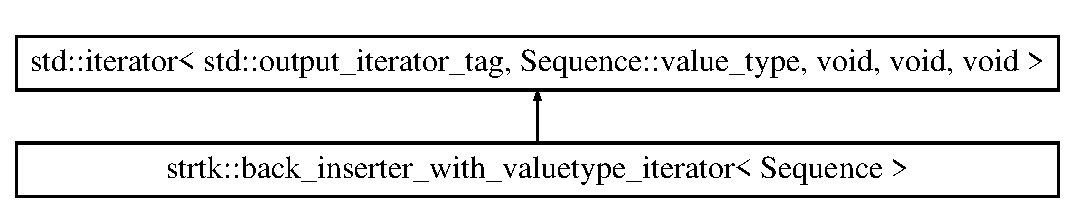
\includegraphics[height=2.000000cm]{classstrtk_1_1back__inserter__with__valuetype__iterator}
\end{center}
\end{figure}
\subsection*{Public Member Functions}
\begin{DoxyCompactItemize}
\item 
\hypertarget{classstrtk_1_1back__inserter__with__valuetype__iterator_a89e3a774ea83fb93775542b6255b1905}{{\bfseries back\-\_\-inserter\-\_\-with\-\_\-valuetype\-\_\-iterator} (Sequence \&sequence)}\label{classstrtk_1_1back__inserter__with__valuetype__iterator_a89e3a774ea83fb93775542b6255b1905}

\item 
\hypertarget{classstrtk_1_1back__inserter__with__valuetype__iterator_a84959fff2894d224f1dae1e5214fcd47}{{\bfseries back\-\_\-inserter\-\_\-with\-\_\-valuetype\-\_\-iterator} (const \hyperlink{classstrtk_1_1back__inserter__with__valuetype__iterator}{back\-\_\-inserter\-\_\-with\-\_\-valuetype\-\_\-iterator} \&itr)}\label{classstrtk_1_1back__inserter__with__valuetype__iterator_a84959fff2894d224f1dae1e5214fcd47}

\item 
\hypertarget{classstrtk_1_1back__inserter__with__valuetype__iterator_a159a36d5ec6bf8b881d568b92f12e9dd}{\hyperlink{classstrtk_1_1back__inserter__with__valuetype__iterator}{back\-\_\-inserter\-\_\-with\-\_\-valuetype\-\_\-iterator} \& {\bfseries operator=} (const \hyperlink{classstrtk_1_1back__inserter__with__valuetype__iterator}{back\-\_\-inserter\-\_\-with\-\_\-valuetype\-\_\-iterator} \&itr)}\label{classstrtk_1_1back__inserter__with__valuetype__iterator_a159a36d5ec6bf8b881d568b92f12e9dd}

\item 
\hypertarget{classstrtk_1_1back__inserter__with__valuetype__iterator_a40c5805ab58a1d2718d9f14bddfeeb69}{\hyperlink{classstrtk_1_1back__inserter__with__valuetype__iterator}{back\-\_\-inserter\-\_\-with\-\_\-valuetype\-\_\-iterator} \& {\bfseries operator=} (const typename Sequence\-::value\-\_\-type \&v)}\label{classstrtk_1_1back__inserter__with__valuetype__iterator_a40c5805ab58a1d2718d9f14bddfeeb69}

\item 
\hypertarget{classstrtk_1_1back__inserter__with__valuetype__iterator_a639cd47c59f1c6a8c7918bb68aa52d4c}{void {\bfseries operator()} (const typename Sequence\-::value\-\_\-type \&v)}\label{classstrtk_1_1back__inserter__with__valuetype__iterator_a639cd47c59f1c6a8c7918bb68aa52d4c}

\item 
\hypertarget{classstrtk_1_1back__inserter__with__valuetype__iterator_a6e4a523e4982e9e80473ba93ebfcb59d}{\hyperlink{classstrtk_1_1back__inserter__with__valuetype__iterator}{back\-\_\-inserter\-\_\-with\-\_\-valuetype\-\_\-iterator} \& {\bfseries operator$\ast$} ()}\label{classstrtk_1_1back__inserter__with__valuetype__iterator_a6e4a523e4982e9e80473ba93ebfcb59d}

\item 
\hypertarget{classstrtk_1_1back__inserter__with__valuetype__iterator_a15f5fe3d9eadea4ead4f4cf36cfc6a52}{\hyperlink{classstrtk_1_1back__inserter__with__valuetype__iterator}{back\-\_\-inserter\-\_\-with\-\_\-valuetype\-\_\-iterator} \& {\bfseries operator++} ()}\label{classstrtk_1_1back__inserter__with__valuetype__iterator_a15f5fe3d9eadea4ead4f4cf36cfc6a52}

\item 
\hypertarget{classstrtk_1_1back__inserter__with__valuetype__iterator_a295a708547f62187ea69eb749eeded9c}{\hyperlink{classstrtk_1_1back__inserter__with__valuetype__iterator}{back\-\_\-inserter\-\_\-with\-\_\-valuetype\-\_\-iterator} {\bfseries operator++} (int)}\label{classstrtk_1_1back__inserter__with__valuetype__iterator_a295a708547f62187ea69eb749eeded9c}

\end{DoxyCompactItemize}


The documentation for this class was generated from the following file\-:\begin{DoxyCompactItemize}
\item 
strtk.\-hpp\end{DoxyCompactItemize}

\hypertarget{classstrtk_1_1base64__to__number__sink}{\section{strtk\-:\-:base64\-\_\-to\-\_\-number\-\_\-sink$<$ T $>$ Class Template Reference}
\label{classstrtk_1_1base64__to__number__sink}\index{strtk\-::base64\-\_\-to\-\_\-number\-\_\-sink$<$ T $>$@{strtk\-::base64\-\_\-to\-\_\-number\-\_\-sink$<$ T $>$}}
}
\subsection*{Public Member Functions}
\begin{DoxyCompactItemize}
\item 
\hypertarget{classstrtk_1_1base64__to__number__sink_ac5cdb8329872d6769a52fe8a720b4044}{{\bfseries base64\-\_\-to\-\_\-number\-\_\-sink} (T \&t)}\label{classstrtk_1_1base64__to__number__sink_ac5cdb8329872d6769a52fe8a720b4044}

\item 
\hypertarget{classstrtk_1_1base64__to__number__sink_a7cfb1605477b334d5aa339f8dce5330d}{{\bfseries base64\-\_\-to\-\_\-number\-\_\-sink} (const \hyperlink{classstrtk_1_1base64__to__number__sink}{base64\-\_\-to\-\_\-number\-\_\-sink} \&bns)}\label{classstrtk_1_1base64__to__number__sink_a7cfb1605477b334d5aa339f8dce5330d}

\item 
\hypertarget{classstrtk_1_1base64__to__number__sink_aba7e6a9cde73b1fcb59e283cb003d6f2}{\hyperlink{classstrtk_1_1base64__to__number__sink}{base64\-\_\-to\-\_\-number\-\_\-sink} \& {\bfseries operator=} (const \hyperlink{classstrtk_1_1base64__to__number__sink}{base64\-\_\-to\-\_\-number\-\_\-sink} \&bns)}\label{classstrtk_1_1base64__to__number__sink_aba7e6a9cde73b1fcb59e283cb003d6f2}

\item 
\hypertarget{classstrtk_1_1base64__to__number__sink_a3b3737d548397ab70a493c11a923b0bf}{\hyperlink{classstrtk_1_1base64__to__number__sink}{base64\-\_\-to\-\_\-number\-\_\-sink} \& {\bfseries operator=} (const std\-::string \&s)}\label{classstrtk_1_1base64__to__number__sink_a3b3737d548397ab70a493c11a923b0bf}

\item 
\hypertarget{classstrtk_1_1base64__to__number__sink_a7b9795d60b0d2065b15ed54bcdd578d2}{{\footnotesize template$<$typename Input\-Iterator $>$ }\\\hyperlink{classstrtk_1_1base64__to__number__sink}{base64\-\_\-to\-\_\-number\-\_\-sink} \& {\bfseries operator=} (const std\-::pair$<$ Input\-Iterator, Input\-Iterator $>$ \&s)}\label{classstrtk_1_1base64__to__number__sink_a7b9795d60b0d2065b15ed54bcdd578d2}

\item 
\hypertarget{classstrtk_1_1base64__to__number__sink_a5bcbbe5ed1680ad2e88d88948e028724}{bool {\bfseries valid} () const }\label{classstrtk_1_1base64__to__number__sink_a5bcbbe5ed1680ad2e88d88948e028724}

\end{DoxyCompactItemize}


The documentation for this class was generated from the following file\-:\begin{DoxyCompactItemize}
\item 
strtk.\-hpp\end{DoxyCompactItemize}

\hypertarget{structstrtk_1_1details_1_1base64__type__tag}{\section{strtk\-:\-:details\-:\-:base64\-\_\-type\-\_\-tag Struct Reference}
\label{structstrtk_1_1details_1_1base64__type__tag}\index{strtk\-::details\-::base64\-\_\-type\-\_\-tag@{strtk\-::details\-::base64\-\_\-type\-\_\-tag}}
}


The documentation for this struct was generated from the following file\-:\begin{DoxyCompactItemize}
\item 
strtk.\-hpp\end{DoxyCompactItemize}

\hypertarget{structstrtk_1_1details_1_1bool__type__tag}{\section{strtk\-:\-:details\-:\-:bool\-\_\-type\-\_\-tag Struct Reference}
\label{structstrtk_1_1details_1_1bool__type__tag}\index{strtk\-::details\-::bool\-\_\-type\-\_\-tag@{strtk\-::details\-::bool\-\_\-type\-\_\-tag}}
}


The documentation for this struct was generated from the following file\-:\begin{DoxyCompactItemize}
\item 
strtk.\-hpp\end{DoxyCompactItemize}

\hypertarget{classstrtk_1_1details_1_1bound__range}{\section{strtk\-:\-:details\-:\-:bound\-\_\-range$<$ Function, Iterator $>$ Class Template Reference}
\label{classstrtk_1_1details_1_1bound__range}\index{strtk\-::details\-::bound\-\_\-range$<$ Function, Iterator $>$@{strtk\-::details\-::bound\-\_\-range$<$ Function, Iterator $>$}}
}
\subsection*{Public Member Functions}
\begin{DoxyCompactItemize}
\item 
\hypertarget{classstrtk_1_1details_1_1bound__range_a57457127d4beb91ed39b31b31ca21fa8}{{\bfseries bound\-\_\-range} (Function f, Iterator first, Iterator last)}\label{classstrtk_1_1details_1_1bound__range_a57457127d4beb91ed39b31b31ca21fa8}

\item 
\hypertarget{classstrtk_1_1details_1_1bound__range_a384a67fa05d11fb882836d49c36f36cd}{void {\bfseries operator()} ()}\label{classstrtk_1_1details_1_1bound__range_a384a67fa05d11fb882836d49c36f36cd}

\end{DoxyCompactItemize}


The documentation for this class was generated from the following file\-:\begin{DoxyCompactItemize}
\item 
strtk.\-hpp\end{DoxyCompactItemize}

\hypertarget{classstrtk_1_1details_1_1bound__range__conditional}{\section{strtk\-:\-:details\-:\-:bound\-\_\-range\-\_\-conditional$<$ Function, Iterator $>$ Class Template Reference}
\label{classstrtk_1_1details_1_1bound__range__conditional}\index{strtk\-::details\-::bound\-\_\-range\-\_\-conditional$<$ Function, Iterator $>$@{strtk\-::details\-::bound\-\_\-range\-\_\-conditional$<$ Function, Iterator $>$}}
}
\subsection*{Public Member Functions}
\begin{DoxyCompactItemize}
\item 
\hypertarget{classstrtk_1_1details_1_1bound__range__conditional_a99b183dde7cc0aa7ee93f9101af12c54}{{\bfseries bound\-\_\-range\-\_\-conditional} (Function f, Iterator first, Iterator last)}\label{classstrtk_1_1details_1_1bound__range__conditional_a99b183dde7cc0aa7ee93f9101af12c54}

\item 
\hypertarget{classstrtk_1_1details_1_1bound__range__conditional_ac1c6004e2a24ae800728cb5ed7f4b753}{bool {\bfseries operator()} ()}\label{classstrtk_1_1details_1_1bound__range__conditional_ac1c6004e2a24ae800728cb5ed7f4b753}

\end{DoxyCompactItemize}


The documentation for this class was generated from the following file\-:\begin{DoxyCompactItemize}
\item 
strtk.\-hpp\end{DoxyCompactItemize}

\hypertarget{classstrtk_1_1build__string}{\section{strtk\-:\-:build\-\_\-string Class Reference}
\label{classstrtk_1_1build__string}\index{strtk\-::build\-\_\-string@{strtk\-::build\-\_\-string}}
}
\subsection*{Public Member Functions}
\begin{DoxyCompactItemize}
\item 
\hypertarget{classstrtk_1_1build__string_a5f1f80fafd748936825a27492e94f55f}{{\bfseries build\-\_\-string} (const std\-::size\-\_\-t \&initial\-\_\-size=64)}\label{classstrtk_1_1build__string_a5f1f80fafd748936825a27492e94f55f}

\item 
\hypertarget{classstrtk_1_1build__string_af31865bd8fd0f0aaabccda8f635b9bb4}{{\footnotesize template$<$typename T $>$ }\\\hyperlink{classstrtk_1_1build__string}{build\-\_\-string} \& {\bfseries operator$<$$<$} (const T \&t)}\label{classstrtk_1_1build__string_af31865bd8fd0f0aaabccda8f635b9bb4}

\item 
\hypertarget{classstrtk_1_1build__string_a5ba3f5b17075185defc635557f44fb5c}{\hyperlink{classstrtk_1_1build__string}{build\-\_\-string} \& {\bfseries operator$<$$<$} (const std\-::string \&s)}\label{classstrtk_1_1build__string_a5ba3f5b17075185defc635557f44fb5c}

\item 
\hypertarget{classstrtk_1_1build__string_a7d77ad6475464e446e010c6b1d047da7}{std\-::string {\bfseries to\-\_\-str} () const }\label{classstrtk_1_1build__string_a7d77ad6475464e446e010c6b1d047da7}

\item 
\hypertarget{classstrtk_1_1build__string_a0425f834a21ae30d73f005f6dae86d05}{{\bfseries operator const char $\ast$} () const }\label{classstrtk_1_1build__string_a0425f834a21ae30d73f005f6dae86d05}

\end{DoxyCompactItemize}


The documentation for this class was generated from the following file\-:\begin{DoxyCompactItemize}
\item 
strtk.\-hpp\end{DoxyCompactItemize}

\hypertarget{structstrtk_1_1details_1_1byte__type__tag}{\section{strtk\-:\-:details\-:\-:byte\-\_\-type\-\_\-tag Struct Reference}
\label{structstrtk_1_1details_1_1byte__type__tag}\index{strtk\-::details\-::byte\-\_\-type\-\_\-tag@{strtk\-::details\-::byte\-\_\-type\-\_\-tag}}
}


The documentation for this struct was generated from the following file\-:\begin{DoxyCompactItemize}
\item 
strtk.\-hpp\end{DoxyCompactItemize}

\hypertarget{structstrtk_1_1details_1_1ca__type}{\section{strtk\-:\-:details\-:\-:ca\-\_\-type$<$ T, is\-\_\-stl\-\_\-container\-\_\-result $>$ Struct Template Reference}
\label{structstrtk_1_1details_1_1ca__type}\index{strtk\-::details\-::ca\-\_\-type$<$ T, is\-\_\-stl\-\_\-container\-\_\-result $>$@{strtk\-::details\-::ca\-\_\-type$<$ T, is\-\_\-stl\-\_\-container\-\_\-result $>$}}
}
\subsection*{Public Types}
\begin{DoxyCompactItemize}
\item 
\hypertarget{structstrtk_1_1details_1_1ca__type_af12f10f2cf8f32103c9ed8ca8e4d00e7}{typedef T \& {\bfseries type}}\label{structstrtk_1_1details_1_1ca__type_af12f10f2cf8f32103c9ed8ca8e4d00e7}

\end{DoxyCompactItemize}


The documentation for this struct was generated from the following file\-:\begin{DoxyCompactItemize}
\item 
strtk.\-hpp\end{DoxyCompactItemize}

\hypertarget{structstrtk_1_1details_1_1ca__type_3_01T_00_01details_1_1yes__t_01_4}{\section{strtk\-:\-:details\-:\-:ca\-\_\-type$<$ T, details\-:\-:yes\-\_\-t $>$ Struct Template Reference}
\label{structstrtk_1_1details_1_1ca__type_3_01T_00_01details_1_1yes__t_01_4}\index{strtk\-::details\-::ca\-\_\-type$<$ T, details\-::yes\-\_\-t $>$@{strtk\-::details\-::ca\-\_\-type$<$ T, details\-::yes\-\_\-t $>$}}
}
\subsection*{Public Types}
\begin{DoxyCompactItemize}
\item 
\hypertarget{structstrtk_1_1details_1_1ca__type_3_01T_00_01details_1_1yes__t_01_4_a8fd647d421fe3f66b17bb60fa9fce174}{typedef \hyperlink{classstrtk_1_1details_1_1container__adder}{details\-::container\-\_\-adder} {\bfseries type}}\label{structstrtk_1_1details_1_1ca__type_3_01T_00_01details_1_1yes__t_01_4_a8fd647d421fe3f66b17bb60fa9fce174}

\end{DoxyCompactItemize}


The documentation for this struct was generated from the following file\-:\begin{DoxyCompactItemize}
\item 
strtk.\-hpp\end{DoxyCompactItemize}

\hypertarget{classstrtk_1_1details_1_1column__selector__base_1_1colsel__value__list}{\section{strtk\-:\-:details\-:\-:column\-\_\-selector\-\_\-base$<$ Cli, N $>$\-:\-:colsel\-\_\-value\-\_\-list Class Reference}
\label{classstrtk_1_1details_1_1column__selector__base_1_1colsel__value__list}\index{strtk\-::details\-::column\-\_\-selector\-\_\-base$<$ Cli, N $>$\-::colsel\-\_\-value\-\_\-list@{strtk\-::details\-::column\-\_\-selector\-\_\-base$<$ Cli, N $>$\-::colsel\-\_\-value\-\_\-list}}
}
\subsection*{Public Types}
\begin{DoxyCompactItemize}
\item 
\hypertarget{classstrtk_1_1details_1_1column__selector__base_1_1colsel__value__list_a0ac46fb0e68f3612a28a1f297d19d8cb}{typedef std\-::pair\\*
$<$ \hyperlink{classstrtk_1_1util_1_1value}{strtk\-::util\-::value}, bool $>$ {\bfseries value\-\_\-t}}\label{classstrtk_1_1details_1_1column__selector__base_1_1colsel__value__list_a0ac46fb0e68f3612a28a1f297d19d8cb}

\end{DoxyCompactItemize}
\subsection*{Public Member Functions}
\begin{DoxyCompactItemize}
\item 
\hypertarget{classstrtk_1_1details_1_1column__selector__base_1_1colsel__value__list_a93492ca8d002d690e8de658ca84fe849}{{\footnotesize template$<$typename T $>$ }\\void {\bfseries register\-\_\-value} (T \&t)}\label{classstrtk_1_1details_1_1column__selector__base_1_1colsel__value__list_a93492ca8d002d690e8de658ca84fe849}

\end{DoxyCompactItemize}
\subsection*{Public Attributes}
\begin{DoxyCompactItemize}
\item 
\hypertarget{classstrtk_1_1details_1_1column__selector__base_1_1colsel__value__list_a9cc9f5a3bbc6c55539a7686bf0af3432}{std\-::size\-\_\-t {\bfseries current\-\_\-index}}\label{classstrtk_1_1details_1_1column__selector__base_1_1colsel__value__list_a9cc9f5a3bbc6c55539a7686bf0af3432}

\item 
\hypertarget{classstrtk_1_1details_1_1column__selector__base_1_1colsel__value__list_aa0b442681593e9a746f85169b87f5c38}{value\-\_\-t {\bfseries value\-\_\-list} \mbox{[}N\mbox{]}}\label{classstrtk_1_1details_1_1column__selector__base_1_1colsel__value__list_aa0b442681593e9a746f85169b87f5c38}

\end{DoxyCompactItemize}


The documentation for this class was generated from the following file\-:\begin{DoxyCompactItemize}
\item 
strtk.\-hpp\end{DoxyCompactItemize}

\hypertarget{structstrtk_1_1details_1_1column__list__impl}{\section{strtk\-:\-:details\-:\-:column\-\_\-list\-\_\-impl$<$ N $>$ Struct Template Reference}
\label{structstrtk_1_1details_1_1column__list__impl}\index{strtk\-::details\-::column\-\_\-list\-\_\-impl$<$ N $>$@{strtk\-::details\-::column\-\_\-list\-\_\-impl$<$ N $>$}}
}
\subsection*{Public Types}
\begin{DoxyCompactItemize}
\item 
enum \{ {\bfseries size} = N
 \}
\end{DoxyCompactItemize}
\subsection*{Public Attributes}
\begin{DoxyCompactItemize}
\item 
\hypertarget{structstrtk_1_1details_1_1column__list__impl_a5bd60e41322f532f02ec28258489419f}{std\-::size\-\_\-t {\bfseries index\-\_\-list} \mbox{[}N\mbox{]}}\label{structstrtk_1_1details_1_1column__list__impl_a5bd60e41322f532f02ec28258489419f}

\end{DoxyCompactItemize}


The documentation for this struct was generated from the following file\-:\begin{DoxyCompactItemize}
\item 
strtk.\-hpp\end{DoxyCompactItemize}

\hypertarget{classstrtk_1_1details_1_1column__selector__base}{\section{strtk\-:\-:details\-:\-:column\-\_\-selector\-\_\-base$<$ Cli, N $>$ Class Template Reference}
\label{classstrtk_1_1details_1_1column__selector__base}\index{strtk\-::details\-::column\-\_\-selector\-\_\-base$<$ Cli, N $>$@{strtk\-::details\-::column\-\_\-selector\-\_\-base$<$ Cli, N $>$}}
}
\subsection*{Classes}
\begin{DoxyCompactItemize}
\item 
class \hyperlink{classstrtk_1_1details_1_1column__selector__base_1_1colsel__value__list}{colsel\-\_\-value\-\_\-list}
\end{DoxyCompactItemize}
\subsection*{Public Types}
\begin{DoxyCompactItemize}
\item 
\hypertarget{classstrtk_1_1details_1_1column__selector__base_aaeb9350cd0b63a5e1555a353ea485c3f}{typedef \hyperlink{classstrtk_1_1details_1_1column__selector__base}{column\-\_\-selector\-\_\-base}\\*
$<$ Cli, N $>$ {\bfseries csb\-\_\-t}}\label{classstrtk_1_1details_1_1column__selector__base_aaeb9350cd0b63a5e1555a353ea485c3f}

\item 
\hypertarget{classstrtk_1_1details_1_1column__selector__base_a5a3c318443405936d314427b5e43da52}{typedef \hyperlink{structstrtk_1_1details_1_1column__list__impl}{column\-\_\-list\-\_\-impl}$<$ N $>$ {\bfseries column\-\_\-list\-\_\-t}}\label{classstrtk_1_1details_1_1column__selector__base_a5a3c318443405936d314427b5e43da52}

\end{DoxyCompactItemize}
\subsection*{Public Member Functions}
\begin{DoxyCompactItemize}
\item 
\hypertarget{classstrtk_1_1details_1_1column__selector__base_a2c9751f9c2f54ead69cab6b00cf31df7}{{\bfseries column\-\_\-selector\-\_\-base} (const \hyperlink{structstrtk_1_1details_1_1column__list__impl}{column\-\_\-list\-\_\-t} \&column\-\_\-list)}\label{classstrtk_1_1details_1_1column__selector__base_a2c9751f9c2f54ead69cab6b00cf31df7}

\item 
\hypertarget{classstrtk_1_1details_1_1column__selector__base_a77297467fc6cd242c9ab73622b59de4b}{\hyperlink{classstrtk_1_1details_1_1column__selector__base}{csb\-\_\-t} \& {\bfseries operator$\ast$} ()}\label{classstrtk_1_1details_1_1column__selector__base_a77297467fc6cd242c9ab73622b59de4b}

\item 
\hypertarget{classstrtk_1_1details_1_1column__selector__base_a3f185265ebba5af503bdb834bfe2ba43}{\hyperlink{classstrtk_1_1details_1_1column__selector__base}{csb\-\_\-t} \& {\bfseries operator++} ()}\label{classstrtk_1_1details_1_1column__selector__base_a3f185265ebba5af503bdb834bfe2ba43}

\item 
\hypertarget{classstrtk_1_1details_1_1column__selector__base_a3dedc2fa37e3f56574297384472d1a6d}{\hyperlink{classstrtk_1_1details_1_1column__selector__base}{csb\-\_\-t} {\bfseries operator++} (int)}\label{classstrtk_1_1details_1_1column__selector__base_a3dedc2fa37e3f56574297384472d1a6d}

\item 
\hypertarget{classstrtk_1_1details_1_1column__selector__base_a6ff2e0c1ea5ea15d1414a6552bd8a334}{{\footnotesize template$<$typename Iterator $>$ }\\\hyperlink{classstrtk_1_1details_1_1column__selector__base}{csb\-\_\-t} \& {\bfseries operator=} (const std\-::pair$<$ Iterator, Iterator $>$ \&r)}\label{classstrtk_1_1details_1_1column__selector__base_a6ff2e0c1ea5ea15d1414a6552bd8a334}

\item 
\hypertarget{classstrtk_1_1details_1_1column__selector__base_a6a43ee8773d86b4ee4d100e856b5db33}{void {\bfseries reset} ()}\label{classstrtk_1_1details_1_1column__selector__base_a6a43ee8773d86b4ee4d100e856b5db33}

\end{DoxyCompactItemize}
\subsection*{Protected Member Functions}
\begin{DoxyCompactItemize}
\item 
\hypertarget{classstrtk_1_1details_1_1column__selector__base_a5feb5ff5c548cdb4865d97f012008546}{{\footnotesize template$<$typename Iterator $>$ }\\void {\bfseries process} (const std\-::pair$<$ Iterator, Iterator $>$ \&r)}\label{classstrtk_1_1details_1_1column__selector__base_a5feb5ff5c548cdb4865d97f012008546}

\item 
\hypertarget{classstrtk_1_1details_1_1column__selector__base_ac2647dda1e834ba10cc1a08b4b96d616}{\hyperlink{classstrtk_1_1details_1_1column__selector__base_1_1colsel__value__list}{colsel\-\_\-value\-\_\-list} \& {\bfseries cvl} ()}\label{classstrtk_1_1details_1_1column__selector__base_ac2647dda1e834ba10cc1a08b4b96d616}

\end{DoxyCompactItemize}
\subsection*{Protected Attributes}
\begin{DoxyCompactItemize}
\item 
\hypertarget{classstrtk_1_1details_1_1column__selector__base_aed847ac1683ee07df619c61b3034b3ae}{const \hyperlink{structstrtk_1_1details_1_1column__list__impl}{column\-\_\-list\-\_\-t} \& {\bfseries column\-\_\-list\-\_\-}}\label{classstrtk_1_1details_1_1column__selector__base_aed847ac1683ee07df619c61b3034b3ae}

\item 
\hypertarget{classstrtk_1_1details_1_1column__selector__base_a54806fb16de171be4fa0d59fadb8876e}{std\-::size\-\_\-t {\bfseries current\-\_\-index\-\_\-}}\label{classstrtk_1_1details_1_1column__selector__base_a54806fb16de171be4fa0d59fadb8876e}

\item 
\hypertarget{classstrtk_1_1details_1_1column__selector__base_a02bd38d732e5f2af11a7bb2d34566b65}{std\-::size\-\_\-t {\bfseries target\-\_\-index\-\_\-}}\label{classstrtk_1_1details_1_1column__selector__base_a02bd38d732e5f2af11a7bb2d34566b65}

\item 
\hypertarget{classstrtk_1_1details_1_1column__selector__base_a739474cd874976cfcaa490a80096ad0a}{std\-::size\-\_\-t {\bfseries col\-\_\-list\-\_\-index\-\_\-}}\label{classstrtk_1_1details_1_1column__selector__base_a739474cd874976cfcaa490a80096ad0a}

\item 
\hypertarget{classstrtk_1_1details_1_1column__selector__base_a790676f26f4409a4b4e00d530bc3b9f2}{std\-::size\-\_\-t {\bfseries error\-\_\-count\-\_\-}}\label{classstrtk_1_1details_1_1column__selector__base_a790676f26f4409a4b4e00d530bc3b9f2}

\item 
\hypertarget{classstrtk_1_1details_1_1column__selector__base_a16a9b0b39f14296d49c4115d4cb10801}{\hyperlink{classstrtk_1_1details_1_1column__selector__base_1_1colsel__value__list}{colsel\-\_\-value\-\_\-list} {\bfseries cvl\-\_\-}}\label{classstrtk_1_1details_1_1column__selector__base_a16a9b0b39f14296d49c4115d4cb10801}

\end{DoxyCompactItemize}


The documentation for this class was generated from the following file\-:\begin{DoxyCompactItemize}
\item 
strtk.\-hpp\end{DoxyCompactItemize}

\hypertarget{classstrtk_1_1details_1_1column__selector__impl}{\section{strtk\-:\-:details\-:\-:column\-\_\-selector\-\_\-impl$<$ T0, T1, T2, T3, T4, T5, T6, T7, T8, T9, T10, T11 $>$ Class Template Reference}
\label{classstrtk_1_1details_1_1column__selector__impl}\index{strtk\-::details\-::column\-\_\-selector\-\_\-impl$<$ T0, T1, T2, T3, T4, T5, T6, T7, T8, T9, T10, T11 $>$@{strtk\-::details\-::column\-\_\-selector\-\_\-impl$<$ T0, T1, T2, T3, T4, T5, T6, T7, T8, T9, T10, T11 $>$}}
}
Inheritance diagram for strtk\-:\-:details\-:\-:column\-\_\-selector\-\_\-impl$<$ T0, T1, T2, T3, T4, T5, T6, T7, T8, T9, T10, T11 $>$\-:\begin{figure}[H]
\begin{center}
\leavevmode
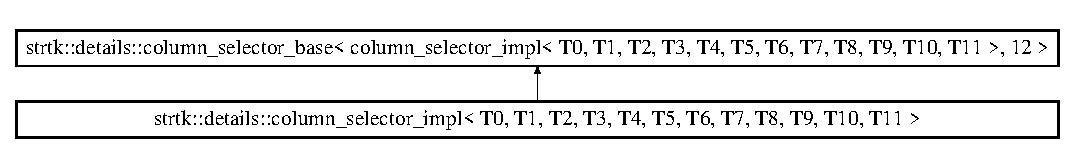
\includegraphics[height=1.623188cm]{classstrtk_1_1details_1_1column__selector__impl}
\end{center}
\end{figure}
\subsection*{Public Types}
\begin{DoxyCompactItemize}
\item 
\hypertarget{classstrtk_1_1details_1_1column__selector__impl_a04649fa5da0c1fcd0c3ed9343fc79395}{typedef \hyperlink{classstrtk_1_1details_1_1column__selector__base}{column\-\_\-selector\-\_\-base}\\*
$<$ \hyperlink{classstrtk_1_1details_1_1column__selector__impl}{column\-\_\-selector\-\_\-impl}$<$ T0, T1, \\*
T2, T3, T4, T5, T6, T7, T8, T9, \\*
T10, T11 $>$, 12 $>$ {\bfseries csb\-\_\-t}}\label{classstrtk_1_1details_1_1column__selector__impl_a04649fa5da0c1fcd0c3ed9343fc79395}

\item 
\hypertarget{classstrtk_1_1details_1_1column__selector__impl_ac2479e8ad60fbe76baf41f5a050d282c}{typedef \hyperlink{structstrtk_1_1details_1_1column__list__impl}{column\-\_\-list\-\_\-impl}$<$ 12 $>$ {\bfseries column\-\_\-list\-\_\-t}}\label{classstrtk_1_1details_1_1column__selector__impl_ac2479e8ad60fbe76baf41f5a050d282c}

\end{DoxyCompactItemize}
\subsection*{Public Member Functions}
\begin{DoxyCompactItemize}
\item 
\hypertarget{classstrtk_1_1details_1_1column__selector__impl_aa3d723ca3b35382ed63613fa80b8292d}{{\bfseries column\-\_\-selector\-\_\-impl} (const \hyperlink{structstrtk_1_1details_1_1column__list__impl}{column\-\_\-list\-\_\-t} \&column\-\_\-list, T0 \&t0, T1 \&t1, T2 \&t2, T3 \&t3, T4 \&t4, T5 \&t5, T6 \&t6, T7 \&t7, T8 \&t8, T9 \&t9, T10 \&t10, T11 \&t11)}\label{classstrtk_1_1details_1_1column__selector__impl_aa3d723ca3b35382ed63613fa80b8292d}

\end{DoxyCompactItemize}
\subsection*{Additional Inherited Members}


The documentation for this class was generated from the following file\-:\begin{DoxyCompactItemize}
\item 
strtk.\-hpp\end{DoxyCompactItemize}

\hypertarget{classstrtk_1_1details_1_1column__selector__impl_3_01T0_01_4}{\section{strtk\-:\-:details\-:\-:column\-\_\-selector\-\_\-impl$<$ T0 $>$ Class Template Reference}
\label{classstrtk_1_1details_1_1column__selector__impl_3_01T0_01_4}\index{strtk\-::details\-::column\-\_\-selector\-\_\-impl$<$ T0 $>$@{strtk\-::details\-::column\-\_\-selector\-\_\-impl$<$ T0 $>$}}
}
Inheritance diagram for strtk\-:\-:details\-:\-:column\-\_\-selector\-\_\-impl$<$ T0 $>$\-:\begin{figure}[H]
\begin{center}
\leavevmode
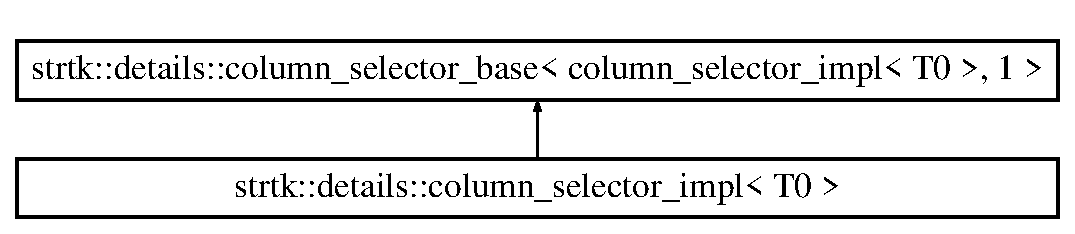
\includegraphics[height=2.000000cm]{classstrtk_1_1details_1_1column__selector__impl_3_01T0_01_4}
\end{center}
\end{figure}
\subsection*{Public Types}
\begin{DoxyCompactItemize}
\item 
\hypertarget{classstrtk_1_1details_1_1column__selector__impl_3_01T0_01_4_af8bba70ca4f43633c82136b7b7799d86}{typedef \hyperlink{classstrtk_1_1details_1_1column__selector__base}{column\-\_\-selector\-\_\-base}\\*
$<$ \hyperlink{classstrtk_1_1details_1_1column__selector__impl}{column\-\_\-selector\-\_\-impl}$<$ T0 $>$, 1 $>$ {\bfseries csb\-\_\-t}}\label{classstrtk_1_1details_1_1column__selector__impl_3_01T0_01_4_af8bba70ca4f43633c82136b7b7799d86}

\item 
\hypertarget{classstrtk_1_1details_1_1column__selector__impl_3_01T0_01_4_a46c8c756ce2c861b489e4ac855676bbb}{typedef \hyperlink{structstrtk_1_1details_1_1column__list__impl}{column\-\_\-list\-\_\-impl}$<$ 1 $>$ {\bfseries column\-\_\-list\-\_\-t}}\label{classstrtk_1_1details_1_1column__selector__impl_3_01T0_01_4_a46c8c756ce2c861b489e4ac855676bbb}

\end{DoxyCompactItemize}
\subsection*{Public Member Functions}
\begin{DoxyCompactItemize}
\item 
\hypertarget{classstrtk_1_1details_1_1column__selector__impl_3_01T0_01_4_a8cb302318ba6880b0c1331823eacd828}{{\bfseries column\-\_\-selector\-\_\-impl} (const \hyperlink{structstrtk_1_1details_1_1column__list__impl}{column\-\_\-list\-\_\-t} \&column\-\_\-list, T0 \&t0)}\label{classstrtk_1_1details_1_1column__selector__impl_3_01T0_01_4_a8cb302318ba6880b0c1331823eacd828}

\end{DoxyCompactItemize}
\subsection*{Additional Inherited Members}


The documentation for this class was generated from the following file\-:\begin{DoxyCompactItemize}
\item 
strtk.\-hpp\end{DoxyCompactItemize}

\hypertarget{classstrtk_1_1details_1_1column__selector__impl_3_01T0_00_01T1_01_4}{\section{strtk\-:\-:details\-:\-:column\-\_\-selector\-\_\-impl$<$ T0, T1 $>$ Class Template Reference}
\label{classstrtk_1_1details_1_1column__selector__impl_3_01T0_00_01T1_01_4}\index{strtk\-::details\-::column\-\_\-selector\-\_\-impl$<$ T0, T1 $>$@{strtk\-::details\-::column\-\_\-selector\-\_\-impl$<$ T0, T1 $>$}}
}
Inheritance diagram for strtk\-:\-:details\-:\-:column\-\_\-selector\-\_\-impl$<$ T0, T1 $>$\-:\begin{figure}[H]
\begin{center}
\leavevmode
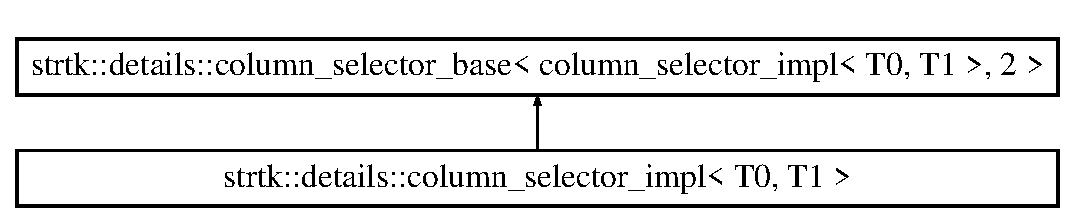
\includegraphics[height=2.000000cm]{classstrtk_1_1details_1_1column__selector__impl_3_01T0_00_01T1_01_4}
\end{center}
\end{figure}
\subsection*{Public Types}
\begin{DoxyCompactItemize}
\item 
\hypertarget{classstrtk_1_1details_1_1column__selector__impl_3_01T0_00_01T1_01_4_ab26ab5124cf582c5354420fdab412701}{typedef \hyperlink{classstrtk_1_1details_1_1column__selector__base}{column\-\_\-selector\-\_\-base}\\*
$<$ \hyperlink{classstrtk_1_1details_1_1column__selector__impl}{column\-\_\-selector\-\_\-impl}$<$ T0, T1 $>$, 2 $>$ {\bfseries csb\-\_\-t}}\label{classstrtk_1_1details_1_1column__selector__impl_3_01T0_00_01T1_01_4_ab26ab5124cf582c5354420fdab412701}

\item 
\hypertarget{classstrtk_1_1details_1_1column__selector__impl_3_01T0_00_01T1_01_4_a1bc4b3c49290d68614d9d5055da41e2a}{typedef \hyperlink{structstrtk_1_1details_1_1column__list__impl}{column\-\_\-list\-\_\-impl}$<$ 2 $>$ {\bfseries column\-\_\-list\-\_\-t}}\label{classstrtk_1_1details_1_1column__selector__impl_3_01T0_00_01T1_01_4_a1bc4b3c49290d68614d9d5055da41e2a}

\end{DoxyCompactItemize}
\subsection*{Public Member Functions}
\begin{DoxyCompactItemize}
\item 
\hypertarget{classstrtk_1_1details_1_1column__selector__impl_3_01T0_00_01T1_01_4_a8cee252b929e109aa2a747751427be7e}{{\bfseries column\-\_\-selector\-\_\-impl} (const \hyperlink{structstrtk_1_1details_1_1column__list__impl}{column\-\_\-list\-\_\-t} \&column\-\_\-list, T1 \&t0, T1 \&t1)}\label{classstrtk_1_1details_1_1column__selector__impl_3_01T0_00_01T1_01_4_a8cee252b929e109aa2a747751427be7e}

\end{DoxyCompactItemize}
\subsection*{Additional Inherited Members}


The documentation for this class was generated from the following file\-:\begin{DoxyCompactItemize}
\item 
strtk.\-hpp\end{DoxyCompactItemize}

\hypertarget{classstrtk_1_1details_1_1column__selector__impl_3_01T0_00_01T1_00_01T2_01_4}{\section{strtk\-:\-:details\-:\-:column\-\_\-selector\-\_\-impl$<$ T0, T1, T2 $>$ Class Template Reference}
\label{classstrtk_1_1details_1_1column__selector__impl_3_01T0_00_01T1_00_01T2_01_4}\index{strtk\-::details\-::column\-\_\-selector\-\_\-impl$<$ T0, T1, T2 $>$@{strtk\-::details\-::column\-\_\-selector\-\_\-impl$<$ T0, T1, T2 $>$}}
}
Inheritance diagram for strtk\-:\-:details\-:\-:column\-\_\-selector\-\_\-impl$<$ T0, T1, T2 $>$\-:\begin{figure}[H]
\begin{center}
\leavevmode
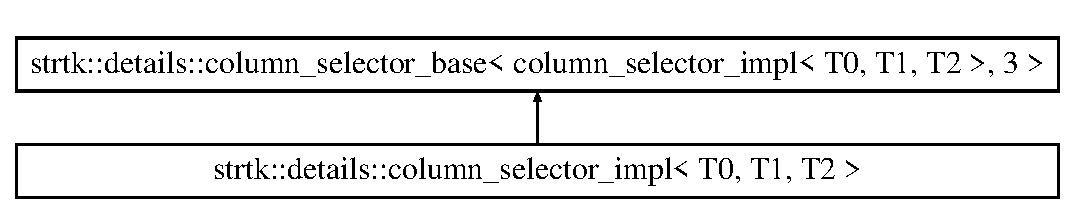
\includegraphics[height=2.000000cm]{classstrtk_1_1details_1_1column__selector__impl_3_01T0_00_01T1_00_01T2_01_4}
\end{center}
\end{figure}
\subsection*{Public Types}
\begin{DoxyCompactItemize}
\item 
\hypertarget{classstrtk_1_1details_1_1column__selector__impl_3_01T0_00_01T1_00_01T2_01_4_a20184aa0473aae996863caf2db79769d}{typedef \hyperlink{classstrtk_1_1details_1_1column__selector__base}{column\-\_\-selector\-\_\-base}\\*
$<$ \hyperlink{classstrtk_1_1details_1_1column__selector__impl}{column\-\_\-selector\-\_\-impl}$<$ T0, T1, \\*
T2 $>$, 3 $>$ {\bfseries csb\-\_\-t}}\label{classstrtk_1_1details_1_1column__selector__impl_3_01T0_00_01T1_00_01T2_01_4_a20184aa0473aae996863caf2db79769d}

\item 
\hypertarget{classstrtk_1_1details_1_1column__selector__impl_3_01T0_00_01T1_00_01T2_01_4_aa9812ea24cceb1f91605878b78410f1a}{typedef \hyperlink{structstrtk_1_1details_1_1column__list__impl}{column\-\_\-list\-\_\-impl}$<$ 3 $>$ {\bfseries column\-\_\-list\-\_\-t}}\label{classstrtk_1_1details_1_1column__selector__impl_3_01T0_00_01T1_00_01T2_01_4_aa9812ea24cceb1f91605878b78410f1a}

\end{DoxyCompactItemize}
\subsection*{Public Member Functions}
\begin{DoxyCompactItemize}
\item 
\hypertarget{classstrtk_1_1details_1_1column__selector__impl_3_01T0_00_01T1_00_01T2_01_4_a8aff7bfbec6ebab2d8a37c80b1ef9f2f}{{\bfseries column\-\_\-selector\-\_\-impl} (const \hyperlink{structstrtk_1_1details_1_1column__list__impl}{column\-\_\-list\-\_\-t} \&column\-\_\-list, T1 \&t0, T1 \&t1, T2 \&t2)}\label{classstrtk_1_1details_1_1column__selector__impl_3_01T0_00_01T1_00_01T2_01_4_a8aff7bfbec6ebab2d8a37c80b1ef9f2f}

\end{DoxyCompactItemize}
\subsection*{Additional Inherited Members}


The documentation for this class was generated from the following file\-:\begin{DoxyCompactItemize}
\item 
strtk.\-hpp\end{DoxyCompactItemize}

\hypertarget{classstrtk_1_1details_1_1column__selector__impl_3_01T0_00_01T1_00_01T2_00_01T3_01_4}{\section{strtk\-:\-:details\-:\-:column\-\_\-selector\-\_\-impl$<$ T0, T1, T2, T3 $>$ Class Template Reference}
\label{classstrtk_1_1details_1_1column__selector__impl_3_01T0_00_01T1_00_01T2_00_01T3_01_4}\index{strtk\-::details\-::column\-\_\-selector\-\_\-impl$<$ T0, T1, T2, T3 $>$@{strtk\-::details\-::column\-\_\-selector\-\_\-impl$<$ T0, T1, T2, T3 $>$}}
}
Inheritance diagram for strtk\-:\-:details\-:\-:column\-\_\-selector\-\_\-impl$<$ T0, T1, T2, T3 $>$\-:\begin{figure}[H]
\begin{center}
\leavevmode
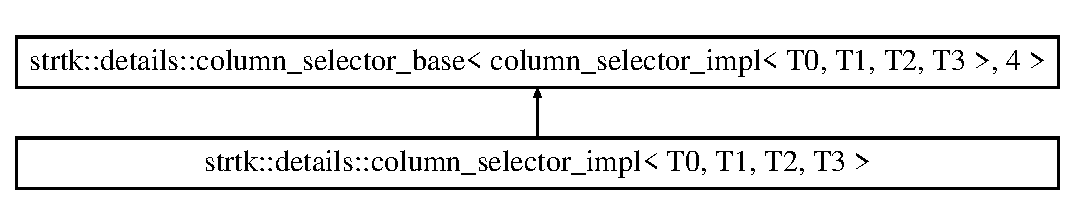
\includegraphics[height=2.000000cm]{classstrtk_1_1details_1_1column__selector__impl_3_01T0_00_01T1_00_01T2_00_01T3_01_4}
\end{center}
\end{figure}
\subsection*{Public Types}
\begin{DoxyCompactItemize}
\item 
\hypertarget{classstrtk_1_1details_1_1column__selector__impl_3_01T0_00_01T1_00_01T2_00_01T3_01_4_ade0c63e3226d37aed45943286e1a83dc}{typedef \hyperlink{classstrtk_1_1details_1_1column__selector__base}{column\-\_\-selector\-\_\-base}\\*
$<$ \hyperlink{classstrtk_1_1details_1_1column__selector__impl}{column\-\_\-selector\-\_\-impl}$<$ T0, T1, \\*
T2, T3 $>$, 4 $>$ {\bfseries csb\-\_\-t}}\label{classstrtk_1_1details_1_1column__selector__impl_3_01T0_00_01T1_00_01T2_00_01T3_01_4_ade0c63e3226d37aed45943286e1a83dc}

\item 
\hypertarget{classstrtk_1_1details_1_1column__selector__impl_3_01T0_00_01T1_00_01T2_00_01T3_01_4_abac4a977ecd01e66368b145caa4ef296}{typedef \hyperlink{structstrtk_1_1details_1_1column__list__impl}{column\-\_\-list\-\_\-impl}$<$ 4 $>$ {\bfseries column\-\_\-list\-\_\-t}}\label{classstrtk_1_1details_1_1column__selector__impl_3_01T0_00_01T1_00_01T2_00_01T3_01_4_abac4a977ecd01e66368b145caa4ef296}

\end{DoxyCompactItemize}
\subsection*{Public Member Functions}
\begin{DoxyCompactItemize}
\item 
\hypertarget{classstrtk_1_1details_1_1column__selector__impl_3_01T0_00_01T1_00_01T2_00_01T3_01_4_ac0c717f4ff5118dc4fa3a8a89f10fd3f}{{\bfseries column\-\_\-selector\-\_\-impl} (const \hyperlink{structstrtk_1_1details_1_1column__list__impl}{column\-\_\-list\-\_\-t} \&column\-\_\-list, T1 \&t0, T1 \&t1, T2 \&t2, T3 \&t3)}\label{classstrtk_1_1details_1_1column__selector__impl_3_01T0_00_01T1_00_01T2_00_01T3_01_4_ac0c717f4ff5118dc4fa3a8a89f10fd3f}

\end{DoxyCompactItemize}
\subsection*{Additional Inherited Members}


The documentation for this class was generated from the following file\-:\begin{DoxyCompactItemize}
\item 
strtk.\-hpp\end{DoxyCompactItemize}

\hypertarget{classstrtk_1_1details_1_1column__selector__impl_3_01T0_00_01T1_00_01T2_00_01T3_00_01T4_01_4}{\section{strtk\-:\-:details\-:\-:column\-\_\-selector\-\_\-impl$<$ T0, T1, T2, T3, T4 $>$ Class Template Reference}
\label{classstrtk_1_1details_1_1column__selector__impl_3_01T0_00_01T1_00_01T2_00_01T3_00_01T4_01_4}\index{strtk\-::details\-::column\-\_\-selector\-\_\-impl$<$ T0, T1, T2, T3, T4 $>$@{strtk\-::details\-::column\-\_\-selector\-\_\-impl$<$ T0, T1, T2, T3, T4 $>$}}
}
Inheritance diagram for strtk\-:\-:details\-:\-:column\-\_\-selector\-\_\-impl$<$ T0, T1, T2, T3, T4 $>$\-:\begin{figure}[H]
\begin{center}
\leavevmode
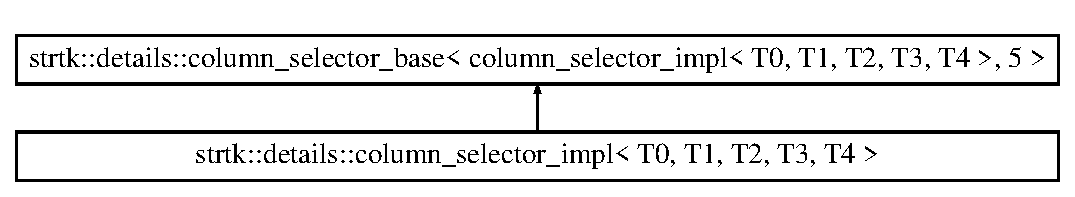
\includegraphics[height=2.000000cm]{classstrtk_1_1details_1_1column__selector__impl_3_01T0_00_01T1_00_01T2_00_01T3_00_01T4_01_4}
\end{center}
\end{figure}
\subsection*{Public Types}
\begin{DoxyCompactItemize}
\item 
\hypertarget{classstrtk_1_1details_1_1column__selector__impl_3_01T0_00_01T1_00_01T2_00_01T3_00_01T4_01_4_a60ba2340e8915b8b5e2312a18080f09b}{typedef \hyperlink{classstrtk_1_1details_1_1column__selector__base}{column\-\_\-selector\-\_\-base}\\*
$<$ \hyperlink{classstrtk_1_1details_1_1column__selector__impl}{column\-\_\-selector\-\_\-impl}$<$ T0, T1, \\*
T2, T3, T4 $>$, 5 $>$ {\bfseries csb\-\_\-t}}\label{classstrtk_1_1details_1_1column__selector__impl_3_01T0_00_01T1_00_01T2_00_01T3_00_01T4_01_4_a60ba2340e8915b8b5e2312a18080f09b}

\item 
\hypertarget{classstrtk_1_1details_1_1column__selector__impl_3_01T0_00_01T1_00_01T2_00_01T3_00_01T4_01_4_aa2e8195741e61d214e687fbc0f304494}{typedef \hyperlink{structstrtk_1_1details_1_1column__list__impl}{column\-\_\-list\-\_\-impl}$<$ 5 $>$ {\bfseries column\-\_\-list\-\_\-t}}\label{classstrtk_1_1details_1_1column__selector__impl_3_01T0_00_01T1_00_01T2_00_01T3_00_01T4_01_4_aa2e8195741e61d214e687fbc0f304494}

\end{DoxyCompactItemize}
\subsection*{Public Member Functions}
\begin{DoxyCompactItemize}
\item 
\hypertarget{classstrtk_1_1details_1_1column__selector__impl_3_01T0_00_01T1_00_01T2_00_01T3_00_01T4_01_4_a684b6909266a8c592b026b1c3fe01d7a}{{\bfseries column\-\_\-selector\-\_\-impl} (const \hyperlink{structstrtk_1_1details_1_1column__list__impl}{column\-\_\-list\-\_\-t} \&column\-\_\-list, T1 \&t0, T1 \&t1, T2 \&t2, T3 \&t3, T4 \&t4)}\label{classstrtk_1_1details_1_1column__selector__impl_3_01T0_00_01T1_00_01T2_00_01T3_00_01T4_01_4_a684b6909266a8c592b026b1c3fe01d7a}

\end{DoxyCompactItemize}
\subsection*{Additional Inherited Members}


The documentation for this class was generated from the following file\-:\begin{DoxyCompactItemize}
\item 
strtk.\-hpp\end{DoxyCompactItemize}

\hypertarget{classstrtk_1_1details_1_1column__selector__impl_3_01T0_00_01T1_00_01T2_00_01T3_00_01T4_00_01T5_01_4}{\section{strtk\-:\-:details\-:\-:column\-\_\-selector\-\_\-impl$<$ T0, T1, T2, T3, T4, T5 $>$ Class Template Reference}
\label{classstrtk_1_1details_1_1column__selector__impl_3_01T0_00_01T1_00_01T2_00_01T3_00_01T4_00_01T5_01_4}\index{strtk\-::details\-::column\-\_\-selector\-\_\-impl$<$ T0, T1, T2, T3, T4, T5 $>$@{strtk\-::details\-::column\-\_\-selector\-\_\-impl$<$ T0, T1, T2, T3, T4, T5 $>$}}
}
Inheritance diagram for strtk\-:\-:details\-:\-:column\-\_\-selector\-\_\-impl$<$ T0, T1, T2, T3, T4, T5 $>$\-:\begin{figure}[H]
\begin{center}
\leavevmode
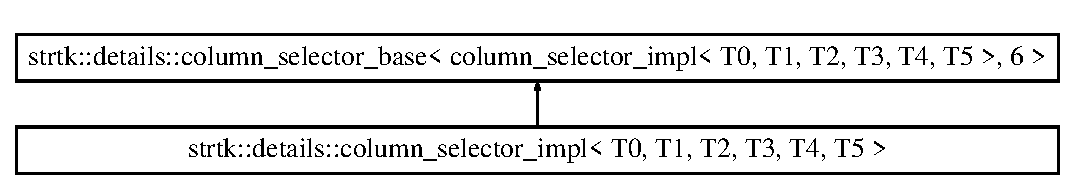
\includegraphics[height=2.000000cm]{classstrtk_1_1details_1_1column__selector__impl_3_01T0_00_01T1_00_01T2_00_01T3_00_01T4_00_01T5_01_4}
\end{center}
\end{figure}
\subsection*{Public Types}
\begin{DoxyCompactItemize}
\item 
\hypertarget{classstrtk_1_1details_1_1column__selector__impl_3_01T0_00_01T1_00_01T2_00_01T3_00_01T4_00_01T5_01_4_adb288ee4815fd4e354dd5aeebbc94a3f}{typedef \hyperlink{classstrtk_1_1details_1_1column__selector__base}{column\-\_\-selector\-\_\-base}\\*
$<$ \hyperlink{classstrtk_1_1details_1_1column__selector__impl}{column\-\_\-selector\-\_\-impl}$<$ T0, T1, \\*
T2, T3, T4, T5 $>$, 6 $>$ {\bfseries csb\-\_\-t}}\label{classstrtk_1_1details_1_1column__selector__impl_3_01T0_00_01T1_00_01T2_00_01T3_00_01T4_00_01T5_01_4_adb288ee4815fd4e354dd5aeebbc94a3f}

\item 
\hypertarget{classstrtk_1_1details_1_1column__selector__impl_3_01T0_00_01T1_00_01T2_00_01T3_00_01T4_00_01T5_01_4_aeba25d7d9ee63caa2e614b3ffedc5304}{typedef \hyperlink{structstrtk_1_1details_1_1column__list__impl}{column\-\_\-list\-\_\-impl}$<$ 6 $>$ {\bfseries column\-\_\-list\-\_\-t}}\label{classstrtk_1_1details_1_1column__selector__impl_3_01T0_00_01T1_00_01T2_00_01T3_00_01T4_00_01T5_01_4_aeba25d7d9ee63caa2e614b3ffedc5304}

\end{DoxyCompactItemize}
\subsection*{Public Member Functions}
\begin{DoxyCompactItemize}
\item 
\hypertarget{classstrtk_1_1details_1_1column__selector__impl_3_01T0_00_01T1_00_01T2_00_01T3_00_01T4_00_01T5_01_4_acf6781afe0d6afc0c2ad8b812cf30c6d}{{\bfseries column\-\_\-selector\-\_\-impl} (const \hyperlink{structstrtk_1_1details_1_1column__list__impl}{column\-\_\-list\-\_\-t} \&column\-\_\-list, T1 \&t0, T1 \&t1, T2 \&t2, T3 \&t3, T4 \&t4, T5 \&t5)}\label{classstrtk_1_1details_1_1column__selector__impl_3_01T0_00_01T1_00_01T2_00_01T3_00_01T4_00_01T5_01_4_acf6781afe0d6afc0c2ad8b812cf30c6d}

\end{DoxyCompactItemize}
\subsection*{Additional Inherited Members}


The documentation for this class was generated from the following file\-:\begin{DoxyCompactItemize}
\item 
strtk.\-hpp\end{DoxyCompactItemize}

\hypertarget{classstrtk_1_1details_1_1column__selector__impl_3_01T0_00_01T1_00_01T2_00_01T3_00_01T4_00_01T5_00_01T6_01_4}{\section{strtk\-:\-:details\-:\-:column\-\_\-selector\-\_\-impl$<$ T0, T1, T2, T3, T4, T5, T6 $>$ Class Template Reference}
\label{classstrtk_1_1details_1_1column__selector__impl_3_01T0_00_01T1_00_01T2_00_01T3_00_01T4_00_01T5_00_01T6_01_4}\index{strtk\-::details\-::column\-\_\-selector\-\_\-impl$<$ T0, T1, T2, T3, T4, T5, T6 $>$@{strtk\-::details\-::column\-\_\-selector\-\_\-impl$<$ T0, T1, T2, T3, T4, T5, T6 $>$}}
}
Inheritance diagram for strtk\-:\-:details\-:\-:column\-\_\-selector\-\_\-impl$<$ T0, T1, T2, T3, T4, T5, T6 $>$\-:\begin{figure}[H]
\begin{center}
\leavevmode
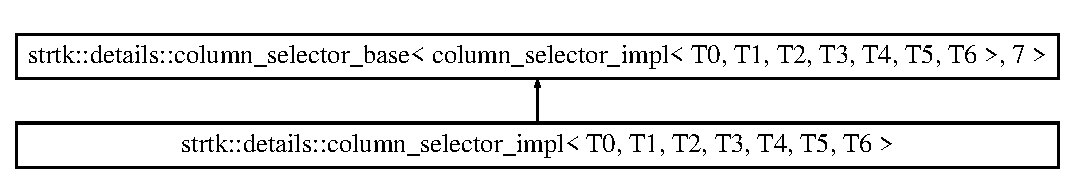
\includegraphics[height=2.000000cm]{classstrtk_1_1details_1_1column__selector__impl_3_01T0_00_01T1_00_01T2_00_01T3_00_01T4_00_01T5_00_01T6_01_4}
\end{center}
\end{figure}
\subsection*{Public Types}
\begin{DoxyCompactItemize}
\item 
\hypertarget{classstrtk_1_1details_1_1column__selector__impl_3_01T0_00_01T1_00_01T2_00_01T3_00_01T4_00_01T5_00_01T6_01_4_af3e044953c2b10f5e928d85182216fbf}{typedef \hyperlink{classstrtk_1_1details_1_1column__selector__base}{column\-\_\-selector\-\_\-base}\\*
$<$ \hyperlink{classstrtk_1_1details_1_1column__selector__impl}{column\-\_\-selector\-\_\-impl}$<$ T0, T1, \\*
T2, T3, T4, T5, T6 $>$, 7 $>$ {\bfseries csb\-\_\-t}}\label{classstrtk_1_1details_1_1column__selector__impl_3_01T0_00_01T1_00_01T2_00_01T3_00_01T4_00_01T5_00_01T6_01_4_af3e044953c2b10f5e928d85182216fbf}

\item 
\hypertarget{classstrtk_1_1details_1_1column__selector__impl_3_01T0_00_01T1_00_01T2_00_01T3_00_01T4_00_01T5_00_01T6_01_4_a19b150cabf3e076d676c1f3564c264d0}{typedef \hyperlink{structstrtk_1_1details_1_1column__list__impl}{column\-\_\-list\-\_\-impl}$<$ 7 $>$ {\bfseries column\-\_\-list\-\_\-t}}\label{classstrtk_1_1details_1_1column__selector__impl_3_01T0_00_01T1_00_01T2_00_01T3_00_01T4_00_01T5_00_01T6_01_4_a19b150cabf3e076d676c1f3564c264d0}

\end{DoxyCompactItemize}
\subsection*{Public Member Functions}
\begin{DoxyCompactItemize}
\item 
\hypertarget{classstrtk_1_1details_1_1column__selector__impl_3_01T0_00_01T1_00_01T2_00_01T3_00_01T4_00_01T5_00_01T6_01_4_aa5030da0ab3ea928ba3e0bc167bd6e04}{{\bfseries column\-\_\-selector\-\_\-impl} (const \hyperlink{structstrtk_1_1details_1_1column__list__impl}{column\-\_\-list\-\_\-t} \&column\-\_\-list, T1 \&t0, T1 \&t1, T2 \&t2, T3 \&t3, T4 \&t4, T5 \&t5, T6 \&t6)}\label{classstrtk_1_1details_1_1column__selector__impl_3_01T0_00_01T1_00_01T2_00_01T3_00_01T4_00_01T5_00_01T6_01_4_aa5030da0ab3ea928ba3e0bc167bd6e04}

\end{DoxyCompactItemize}
\subsection*{Additional Inherited Members}


The documentation for this class was generated from the following file\-:\begin{DoxyCompactItemize}
\item 
strtk.\-hpp\end{DoxyCompactItemize}

\hypertarget{classstrtk_1_1details_1_1column__selector__impl_3_01T0_00_01T1_00_01T2_00_01T3_00_01T4_00_01T5_00_01T6_00_01T7_01_4}{\section{strtk\-:\-:details\-:\-:column\-\_\-selector\-\_\-impl$<$ T0, T1, T2, T3, T4, T5, T6, T7 $>$ Class Template Reference}
\label{classstrtk_1_1details_1_1column__selector__impl_3_01T0_00_01T1_00_01T2_00_01T3_00_01T4_00_01T5_00_01T6_00_01T7_01_4}\index{strtk\-::details\-::column\-\_\-selector\-\_\-impl$<$ T0, T1, T2, T3, T4, T5, T6, T7 $>$@{strtk\-::details\-::column\-\_\-selector\-\_\-impl$<$ T0, T1, T2, T3, T4, T5, T6, T7 $>$}}
}
Inheritance diagram for strtk\-:\-:details\-:\-:column\-\_\-selector\-\_\-impl$<$ T0, T1, T2, T3, T4, T5, T6, T7 $>$\-:\begin{figure}[H]
\begin{center}
\leavevmode
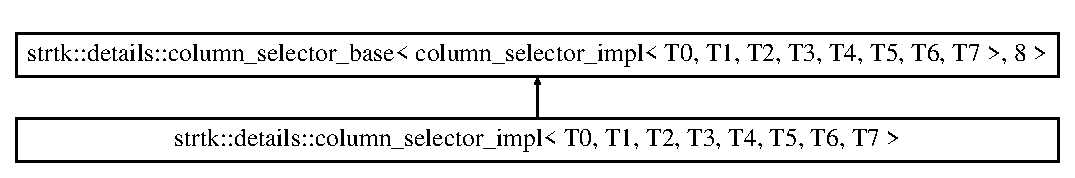
\includegraphics[height=1.941074cm]{classstrtk_1_1details_1_1column__selector__impl_3_01T0_00_01T1_00_01T2_00_01T3_00_01T4_00_01T5_00_01T6_00_01T7_01_4}
\end{center}
\end{figure}
\subsection*{Public Types}
\begin{DoxyCompactItemize}
\item 
\hypertarget{classstrtk_1_1details_1_1column__selector__impl_3_01T0_00_01T1_00_01T2_00_01T3_00_01T4_00_01T5_00_01T6_00_01T7_01_4_a3a61e9531d8c27622e84379a27b90bde}{typedef \hyperlink{classstrtk_1_1details_1_1column__selector__base}{column\-\_\-selector\-\_\-base}\\*
$<$ \hyperlink{classstrtk_1_1details_1_1column__selector__impl}{column\-\_\-selector\-\_\-impl}$<$ T0, T1, \\*
T2, T3, T4, T5, T6, T7 $>$, 8 $>$ {\bfseries csb\-\_\-t}}\label{classstrtk_1_1details_1_1column__selector__impl_3_01T0_00_01T1_00_01T2_00_01T3_00_01T4_00_01T5_00_01T6_00_01T7_01_4_a3a61e9531d8c27622e84379a27b90bde}

\item 
\hypertarget{classstrtk_1_1details_1_1column__selector__impl_3_01T0_00_01T1_00_01T2_00_01T3_00_01T4_00_01T5_00_01T6_00_01T7_01_4_a47aa3a31e69f8e1f080704ece3fdff3d}{typedef \hyperlink{structstrtk_1_1details_1_1column__list__impl}{column\-\_\-list\-\_\-impl}$<$ 8 $>$ {\bfseries column\-\_\-list\-\_\-t}}\label{classstrtk_1_1details_1_1column__selector__impl_3_01T0_00_01T1_00_01T2_00_01T3_00_01T4_00_01T5_00_01T6_00_01T7_01_4_a47aa3a31e69f8e1f080704ece3fdff3d}

\end{DoxyCompactItemize}
\subsection*{Public Member Functions}
\begin{DoxyCompactItemize}
\item 
\hypertarget{classstrtk_1_1details_1_1column__selector__impl_3_01T0_00_01T1_00_01T2_00_01T3_00_01T4_00_01T5_00_01T6_00_01T7_01_4_a19fc6c09ea90bcb1d06f2122e08e9a37}{{\bfseries column\-\_\-selector\-\_\-impl} (const \hyperlink{structstrtk_1_1details_1_1column__list__impl}{column\-\_\-list\-\_\-t} \&column\-\_\-list, T1 \&t0, T1 \&t1, T2 \&t2, T3 \&t3, T4 \&t4, T5 \&t5, T6 \&t6, T7 \&t7)}\label{classstrtk_1_1details_1_1column__selector__impl_3_01T0_00_01T1_00_01T2_00_01T3_00_01T4_00_01T5_00_01T6_00_01T7_01_4_a19fc6c09ea90bcb1d06f2122e08e9a37}

\end{DoxyCompactItemize}
\subsection*{Additional Inherited Members}


The documentation for this class was generated from the following file\-:\begin{DoxyCompactItemize}
\item 
strtk.\-hpp\end{DoxyCompactItemize}

\hypertarget{classstrtk_1_1details_1_1column__selector__impl_3_01T0_00_01T1_00_01T2_00_01T3_00_01T4_00_01T5_00_01T6_00_01T7_00_01T8_01_4}{\section{strtk\-:\-:details\-:\-:column\-\_\-selector\-\_\-impl$<$ T0, T1, T2, T3, T4, T5, T6, T7, T8 $>$ Class Template Reference}
\label{classstrtk_1_1details_1_1column__selector__impl_3_01T0_00_01T1_00_01T2_00_01T3_00_01T4_00_01T5_00_01T6_00_01T7_00_01T8_01_4}\index{strtk\-::details\-::column\-\_\-selector\-\_\-impl$<$ T0, T1, T2, T3, T4, T5, T6, T7, T8 $>$@{strtk\-::details\-::column\-\_\-selector\-\_\-impl$<$ T0, T1, T2, T3, T4, T5, T6, T7, T8 $>$}}
}
Inheritance diagram for strtk\-:\-:details\-:\-:column\-\_\-selector\-\_\-impl$<$ T0, T1, T2, T3, T4, T5, T6, T7, T8 $>$\-:\begin{figure}[H]
\begin{center}
\leavevmode
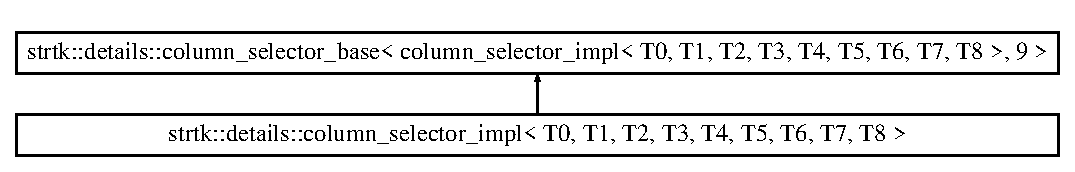
\includegraphics[height=1.866667cm]{classstrtk_1_1details_1_1column__selector__impl_3_01T0_00_01T1_00_01T2_00_01T3_00_01T4_00_01T5_00_01T6_00_01T7_00_01T8_01_4}
\end{center}
\end{figure}
\subsection*{Public Types}
\begin{DoxyCompactItemize}
\item 
\hypertarget{classstrtk_1_1details_1_1column__selector__impl_3_01T0_00_01T1_00_01T2_00_01T3_00_01T4_00_01T5_00_01T6_00_01T7_00_01T8_01_4_a2c8bb80c9397891b76c9e05c9b0cb63d}{typedef \hyperlink{classstrtk_1_1details_1_1column__selector__base}{column\-\_\-selector\-\_\-base}\\*
$<$ \hyperlink{classstrtk_1_1details_1_1column__selector__impl}{column\-\_\-selector\-\_\-impl}$<$ T0, T1, \\*
T2, T3, T4, T5, T6, T7, T8 $>$, 9 $>$ {\bfseries csb\-\_\-t}}\label{classstrtk_1_1details_1_1column__selector__impl_3_01T0_00_01T1_00_01T2_00_01T3_00_01T4_00_01T5_00_01T6_00_01T7_00_01T8_01_4_a2c8bb80c9397891b76c9e05c9b0cb63d}

\item 
\hypertarget{classstrtk_1_1details_1_1column__selector__impl_3_01T0_00_01T1_00_01T2_00_01T3_00_01T4_00_01T5_00_01T6_00_01T7_00_01T8_01_4_abcc7b8cad8fb5f3665de184460092353}{typedef \hyperlink{structstrtk_1_1details_1_1column__list__impl}{column\-\_\-list\-\_\-impl}$<$ 9 $>$ {\bfseries column\-\_\-list\-\_\-t}}\label{classstrtk_1_1details_1_1column__selector__impl_3_01T0_00_01T1_00_01T2_00_01T3_00_01T4_00_01T5_00_01T6_00_01T7_00_01T8_01_4_abcc7b8cad8fb5f3665de184460092353}

\end{DoxyCompactItemize}
\subsection*{Public Member Functions}
\begin{DoxyCompactItemize}
\item 
\hypertarget{classstrtk_1_1details_1_1column__selector__impl_3_01T0_00_01T1_00_01T2_00_01T3_00_01T4_00_01T5_00_01T6_00_01T7_00_01T8_01_4_ae146b8d110e2891e08401758b76db748}{{\bfseries column\-\_\-selector\-\_\-impl} (const \hyperlink{structstrtk_1_1details_1_1column__list__impl}{column\-\_\-list\-\_\-t} \&column\-\_\-list, T1 \&t0, T1 \&t1, T2 \&t2, T3 \&t3, T4 \&t4, T5 \&t5, T6 \&t6, T7 \&t7, T8 \&t8)}\label{classstrtk_1_1details_1_1column__selector__impl_3_01T0_00_01T1_00_01T2_00_01T3_00_01T4_00_01T5_00_01T6_00_01T7_00_01T8_01_4_ae146b8d110e2891e08401758b76db748}

\end{DoxyCompactItemize}
\subsection*{Additional Inherited Members}


The documentation for this class was generated from the following file\-:\begin{DoxyCompactItemize}
\item 
strtk.\-hpp\end{DoxyCompactItemize}

\hypertarget{classstrtk_1_1details_1_1column__selector__impl_3_01T0_00_01T1_00_01T2_00_01T3_00_01T4_00_01T5_043b13d3d6fe5ff73160afdc979d62aa7}{\section{strtk\-:\-:details\-:\-:column\-\_\-selector\-\_\-impl$<$ T0, T1, T2, T3, T4, T5, T6, T7, T8, T9 $>$ Class Template Reference}
\label{classstrtk_1_1details_1_1column__selector__impl_3_01T0_00_01T1_00_01T2_00_01T3_00_01T4_00_01T5_043b13d3d6fe5ff73160afdc979d62aa7}\index{strtk\-::details\-::column\-\_\-selector\-\_\-impl$<$ T0, T1, T2, T3, T4, T5, T6, T7, T8, T9 $>$@{strtk\-::details\-::column\-\_\-selector\-\_\-impl$<$ T0, T1, T2, T3, T4, T5, T6, T7, T8, T9 $>$}}
}
Inheritance diagram for strtk\-:\-:details\-:\-:column\-\_\-selector\-\_\-impl$<$ T0, T1, T2, T3, T4, T5, T6, T7, T8, T9 $>$\-:\begin{figure}[H]
\begin{center}
\leavevmode
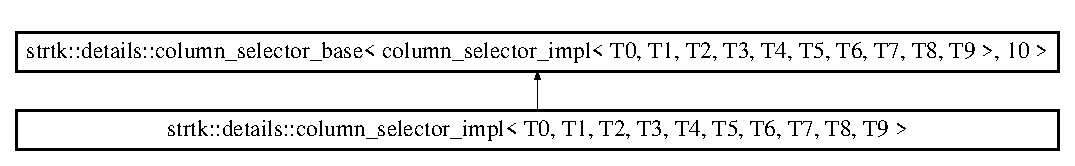
\includegraphics[height=1.777778cm]{classstrtk_1_1details_1_1column__selector__impl_3_01T0_00_01T1_00_01T2_00_01T3_00_01T4_00_01T5_043b13d3d6fe5ff73160afdc979d62aa7}
\end{center}
\end{figure}
\subsection*{Public Types}
\begin{DoxyCompactItemize}
\item 
\hypertarget{classstrtk_1_1details_1_1column__selector__impl_3_01T0_00_01T1_00_01T2_00_01T3_00_01T4_00_01T5_043b13d3d6fe5ff73160afdc979d62aa7_ab24c850f36ea332c2a040f9c60a4d6ae}{typedef \hyperlink{classstrtk_1_1details_1_1column__selector__base}{column\-\_\-selector\-\_\-base}\\*
$<$ \hyperlink{classstrtk_1_1details_1_1column__selector__impl}{column\-\_\-selector\-\_\-impl}$<$ T0, T1, \\*
T2, T3, T4, T5, T6, T7, T8, T9 $>$, 10 $>$ {\bfseries csb\-\_\-t}}\label{classstrtk_1_1details_1_1column__selector__impl_3_01T0_00_01T1_00_01T2_00_01T3_00_01T4_00_01T5_043b13d3d6fe5ff73160afdc979d62aa7_ab24c850f36ea332c2a040f9c60a4d6ae}

\item 
\hypertarget{classstrtk_1_1details_1_1column__selector__impl_3_01T0_00_01T1_00_01T2_00_01T3_00_01T4_00_01T5_043b13d3d6fe5ff73160afdc979d62aa7_a6bd359b0ec12eb422bce47ef309cb8c1}{typedef \hyperlink{structstrtk_1_1details_1_1column__list__impl}{column\-\_\-list\-\_\-impl}$<$ 10 $>$ {\bfseries column\-\_\-list\-\_\-t}}\label{classstrtk_1_1details_1_1column__selector__impl_3_01T0_00_01T1_00_01T2_00_01T3_00_01T4_00_01T5_043b13d3d6fe5ff73160afdc979d62aa7_a6bd359b0ec12eb422bce47ef309cb8c1}

\end{DoxyCompactItemize}
\subsection*{Public Member Functions}
\begin{DoxyCompactItemize}
\item 
\hypertarget{classstrtk_1_1details_1_1column__selector__impl_3_01T0_00_01T1_00_01T2_00_01T3_00_01T4_00_01T5_043b13d3d6fe5ff73160afdc979d62aa7_ae5f2b9b0fd57487134745b844dd731af}{{\bfseries column\-\_\-selector\-\_\-impl} (const \hyperlink{structstrtk_1_1details_1_1column__list__impl}{column\-\_\-list\-\_\-t} \&column\-\_\-list, T1 \&t0, T1 \&t1, T2 \&t2, T3 \&t3, T4 \&t4, T5 \&t5, T6 \&t6, T7 \&t7, T8 \&t8, T9 \&t9)}\label{classstrtk_1_1details_1_1column__selector__impl_3_01T0_00_01T1_00_01T2_00_01T3_00_01T4_00_01T5_043b13d3d6fe5ff73160afdc979d62aa7_ae5f2b9b0fd57487134745b844dd731af}

\end{DoxyCompactItemize}
\subsection*{Additional Inherited Members}


The documentation for this class was generated from the following file\-:\begin{DoxyCompactItemize}
\item 
strtk.\-hpp\end{DoxyCompactItemize}

\hypertarget{classstrtk_1_1details_1_1column__selector__impl_3_01T0_00_01T1_00_01T2_00_01T3_00_01T4_00_01T5_0c1c6bb8abfc5930b575d229537727fec}{\section{strtk\-:\-:details\-:\-:column\-\_\-selector\-\_\-impl$<$ T0, T1, T2, T3, T4, T5, T6, T7, T8, T9, T10 $>$ Class Template Reference}
\label{classstrtk_1_1details_1_1column__selector__impl_3_01T0_00_01T1_00_01T2_00_01T3_00_01T4_00_01T5_0c1c6bb8abfc5930b575d229537727fec}\index{strtk\-::details\-::column\-\_\-selector\-\_\-impl$<$ T0, T1, T2, T3, T4, T5, T6, T7, T8, T9, T10 $>$@{strtk\-::details\-::column\-\_\-selector\-\_\-impl$<$ T0, T1, T2, T3, T4, T5, T6, T7, T8, T9, T10 $>$}}
}
Inheritance diagram for strtk\-:\-:details\-:\-:column\-\_\-selector\-\_\-impl$<$ T0, T1, T2, T3, T4, T5, T6, T7, T8, T9, T10 $>$\-:\begin{figure}[H]
\begin{center}
\leavevmode
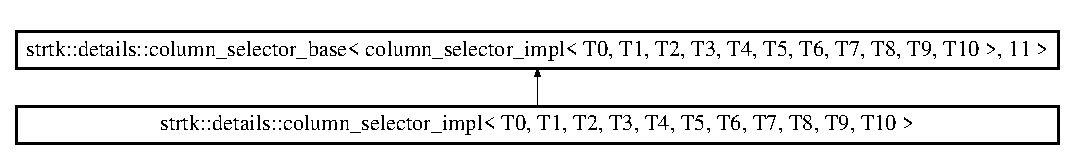
\includegraphics[height=1.696970cm]{classstrtk_1_1details_1_1column__selector__impl_3_01T0_00_01T1_00_01T2_00_01T3_00_01T4_00_01T5_0c1c6bb8abfc5930b575d229537727fec}
\end{center}
\end{figure}
\subsection*{Public Types}
\begin{DoxyCompactItemize}
\item 
\hypertarget{classstrtk_1_1details_1_1column__selector__impl_3_01T0_00_01T1_00_01T2_00_01T3_00_01T4_00_01T5_0c1c6bb8abfc5930b575d229537727fec_adf496ec49826d8934570379581e134bc}{typedef \hyperlink{classstrtk_1_1details_1_1column__selector__base}{column\-\_\-selector\-\_\-base}\\*
$<$ \hyperlink{classstrtk_1_1details_1_1column__selector__impl}{column\-\_\-selector\-\_\-impl}$<$ T0, T1, \\*
T2, T3, T4, T5, T6, T7, T8, T9, \\*
T10 $>$, 11 $>$ {\bfseries csb\-\_\-t}}\label{classstrtk_1_1details_1_1column__selector__impl_3_01T0_00_01T1_00_01T2_00_01T3_00_01T4_00_01T5_0c1c6bb8abfc5930b575d229537727fec_adf496ec49826d8934570379581e134bc}

\item 
\hypertarget{classstrtk_1_1details_1_1column__selector__impl_3_01T0_00_01T1_00_01T2_00_01T3_00_01T4_00_01T5_0c1c6bb8abfc5930b575d229537727fec_af64aa1bceabcd372d3c06dba7d34d31c}{typedef \hyperlink{structstrtk_1_1details_1_1column__list__impl}{column\-\_\-list\-\_\-impl}$<$ 11 $>$ {\bfseries column\-\_\-list\-\_\-t}}\label{classstrtk_1_1details_1_1column__selector__impl_3_01T0_00_01T1_00_01T2_00_01T3_00_01T4_00_01T5_0c1c6bb8abfc5930b575d229537727fec_af64aa1bceabcd372d3c06dba7d34d31c}

\end{DoxyCompactItemize}
\subsection*{Public Member Functions}
\begin{DoxyCompactItemize}
\item 
\hypertarget{classstrtk_1_1details_1_1column__selector__impl_3_01T0_00_01T1_00_01T2_00_01T3_00_01T4_00_01T5_0c1c6bb8abfc5930b575d229537727fec_ab511b82c96e5c3f45a16ab8050902ba1}{{\bfseries column\-\_\-selector\-\_\-impl} (const \hyperlink{structstrtk_1_1details_1_1column__list__impl}{column\-\_\-list\-\_\-t} \&column\-\_\-list, T0 \&t0, T1 \&t1, T2 \&t2, T3 \&t3, T4 \&t4, T5 \&t5, T6 \&t6, T7 \&t7, T8 \&t8, T9 \&t9, T10 \&t10)}\label{classstrtk_1_1details_1_1column__selector__impl_3_01T0_00_01T1_00_01T2_00_01T3_00_01T4_00_01T5_0c1c6bb8abfc5930b575d229537727fec_ab511b82c96e5c3f45a16ab8050902ba1}

\end{DoxyCompactItemize}
\subsection*{Additional Inherited Members}


The documentation for this class was generated from the following file\-:\begin{DoxyCompactItemize}
\item 
strtk.\-hpp\end{DoxyCompactItemize}

\hypertarget{classstrtk_1_1details_1_1column__selector__iterator__impl}{\section{strtk\-:\-:details\-:\-:column\-\_\-selector\-\_\-iterator\-\_\-impl$<$ Input\-Iterator, N $>$ Class Template Reference}
\label{classstrtk_1_1details_1_1column__selector__iterator__impl}\index{strtk\-::details\-::column\-\_\-selector\-\_\-iterator\-\_\-impl$<$ Input\-Iterator, N $>$@{strtk\-::details\-::column\-\_\-selector\-\_\-iterator\-\_\-impl$<$ Input\-Iterator, N $>$}}
}
\subsection*{Public Types}
\begin{DoxyCompactItemize}
\item 
\hypertarget{classstrtk_1_1details_1_1column__selector__iterator__impl_a8953537eafbd503e85d8de9e5aca7d78}{typedef \\*
\hyperlink{classstrtk_1_1details_1_1column__selector__iterator__impl}{column\-\_\-selector\-\_\-iterator\-\_\-impl}\\*
$<$ Input\-Iterator, N $>$ {\bfseries csii\-\_\-t}}\label{classstrtk_1_1details_1_1column__selector__iterator__impl_a8953537eafbd503e85d8de9e5aca7d78}

\item 
\hypertarget{classstrtk_1_1details_1_1column__selector__iterator__impl_a9bd3ac882814bdd99558a285d49f3b2c}{typedef \\*
\hyperlink{structstrtk_1_1details_1_1column__list__impl}{details\-::column\-\_\-list\-\_\-impl}$<$ N $>$ {\bfseries column\-\_\-list\-\_\-t}}\label{classstrtk_1_1details_1_1column__selector__iterator__impl_a9bd3ac882814bdd99558a285d49f3b2c}

\item 
\hypertarget{classstrtk_1_1details_1_1column__selector__iterator__impl_a4d8fec152843941b158e97f4a714c506}{typedef std\-::pair\\*
$<$ Input\-Iterator, Input\-Iterator $>$ {\bfseries iterator\-\_\-type}}\label{classstrtk_1_1details_1_1column__selector__iterator__impl_a4d8fec152843941b158e97f4a714c506}

\item 
\hypertarget{classstrtk_1_1details_1_1column__selector__iterator__impl_adc63fc56bdeb7537aa646a8ed0177b55}{typedef iterator\-\_\-type $\ast$ {\bfseries iterator\-\_\-type\-\_\-ptr}}\label{classstrtk_1_1details_1_1column__selector__iterator__impl_adc63fc56bdeb7537aa646a8ed0177b55}

\end{DoxyCompactItemize}
\subsection*{Public Member Functions}
\begin{DoxyCompactItemize}
\item 
\hypertarget{classstrtk_1_1details_1_1column__selector__iterator__impl_a97eeab10ab785b897e0d090df7e5a9b7}{{\bfseries column\-\_\-selector\-\_\-iterator\-\_\-impl} (const \hyperlink{structstrtk_1_1details_1_1column__list__impl}{details\-::column\-\_\-list\-\_\-impl}$<$ N $>$ \&column\-\_\-list, iterator\-\_\-type(\&token\-\_\-list)\mbox{[}N\mbox{]})}\label{classstrtk_1_1details_1_1column__selector__iterator__impl_a97eeab10ab785b897e0d090df7e5a9b7}

\item 
\hypertarget{classstrtk_1_1details_1_1column__selector__iterator__impl_a446e250fa563f418c3175f744dcf0323}{\hyperlink{classstrtk_1_1details_1_1column__selector__iterator__impl}{csii\-\_\-t} \& {\bfseries operator$\ast$} ()}\label{classstrtk_1_1details_1_1column__selector__iterator__impl_a446e250fa563f418c3175f744dcf0323}

\item 
\hypertarget{classstrtk_1_1details_1_1column__selector__iterator__impl_a490201349a76e2a0878f6affb540efe2}{\hyperlink{classstrtk_1_1details_1_1column__selector__iterator__impl}{csii\-\_\-t} \& {\bfseries operator++} ()}\label{classstrtk_1_1details_1_1column__selector__iterator__impl_a490201349a76e2a0878f6affb540efe2}

\item 
\hypertarget{classstrtk_1_1details_1_1column__selector__iterator__impl_a11e1966cf9e1b1a3604a82e524cab7dd}{\hyperlink{classstrtk_1_1details_1_1column__selector__iterator__impl}{csii\-\_\-t} {\bfseries operator++} (int)}\label{classstrtk_1_1details_1_1column__selector__iterator__impl_a11e1966cf9e1b1a3604a82e524cab7dd}

\item 
\hypertarget{classstrtk_1_1details_1_1column__selector__iterator__impl_a4b83b5e3acdb2bb92c7f79e60c989de7}{{\footnotesize template$<$typename Iterator $>$ }\\\hyperlink{classstrtk_1_1details_1_1column__selector__iterator__impl}{csii\-\_\-t} \& {\bfseries operator=} (const std\-::pair$<$ Iterator, Iterator $>$ \&r)}\label{classstrtk_1_1details_1_1column__selector__iterator__impl_a4b83b5e3acdb2bb92c7f79e60c989de7}

\end{DoxyCompactItemize}


The documentation for this class was generated from the following file\-:\begin{DoxyCompactItemize}
\item 
strtk.\-hpp\end{DoxyCompactItemize}

\hypertarget{classstrtk_1_1combination__iterator}{\section{strtk\-:\-:combination\-\_\-iterator$<$ Iterator $>$ Class Template Reference}
\label{classstrtk_1_1combination__iterator}\index{strtk\-::combination\-\_\-iterator$<$ Iterator $>$@{strtk\-::combination\-\_\-iterator$<$ Iterator $>$}}
}
Inheritance diagram for strtk\-:\-:combination\-\_\-iterator$<$ Iterator $>$\-:\begin{figure}[H]
\begin{center}
\leavevmode
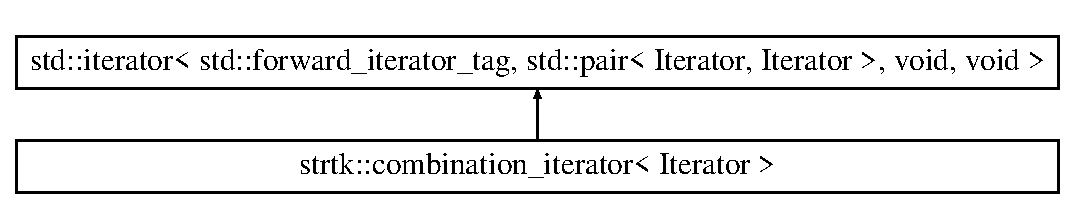
\includegraphics[height=2.000000cm]{classstrtk_1_1combination__iterator}
\end{center}
\end{figure}
\subsection*{Public Types}
\begin{DoxyCompactItemize}
\item 
\hypertarget{classstrtk_1_1combination__iterator_a23555e9b85d322844788910a29d5df9d}{typedef Iterator {\bfseries iterator}}\label{classstrtk_1_1combination__iterator_a23555e9b85d322844788910a29d5df9d}

\item 
\hypertarget{classstrtk_1_1combination__iterator_a1e945ae333f2e40a729f5d70104cdb7e}{typedef const iterator {\bfseries const\-\_\-iterator}}\label{classstrtk_1_1combination__iterator_a1e945ae333f2e40a729f5d70104cdb7e}

\item 
\hypertarget{classstrtk_1_1combination__iterator_acad4b059bcc059577cc09e001555c176}{typedef std\-::pair$<$ Iterator, \\*
Iterator $>$ {\bfseries range\-\_\-type}}\label{classstrtk_1_1combination__iterator_acad4b059bcc059577cc09e001555c176}

\end{DoxyCompactItemize}
\subsection*{Public Member Functions}
\begin{DoxyCompactItemize}
\item 
\hypertarget{classstrtk_1_1combination__iterator_a3ff96c3eb259eba138d6618cef146824}{{\bfseries combination\-\_\-iterator} (const std\-::size\-\_\-t \&k, iterator begin, iterator end, const bool sorted=true)}\label{classstrtk_1_1combination__iterator_a3ff96c3eb259eba138d6618cef146824}

\item 
\hypertarget{classstrtk_1_1combination__iterator_ae511b7bc0d36650c6d57fc92d4d6a07a}{{\footnotesize template$<$typename T , typename Allocator , template$<$ typename, typename $>$ class Sequence$>$ }\\{\bfseries combination\-\_\-iterator} (const std\-::size\-\_\-t \&k, Sequence$<$ T, Allocator $>$ \&seq, const bool sorted=true)}\label{classstrtk_1_1combination__iterator_ae511b7bc0d36650c6d57fc92d4d6a07a}

\item 
\hypertarget{classstrtk_1_1combination__iterator_a45dc3c0696583fd08d465837202bcdb5}{{\bfseries combination\-\_\-iterator} (const std\-::size\-\_\-t \&k, std\-::string \&str, const bool sorted=true)}\label{classstrtk_1_1combination__iterator_a45dc3c0696583fd08d465837202bcdb5}

\item 
\hypertarget{classstrtk_1_1combination__iterator_a4124f837ef476c0e13aa3555f22b1160}{{\bfseries combination\-\_\-iterator} (iterator end)}\label{classstrtk_1_1combination__iterator_a4124f837ef476c0e13aa3555f22b1160}

\item 
\hypertarget{classstrtk_1_1combination__iterator_aef5b80423e9025d7c20767e2f3598f18}{{\bfseries combination\-\_\-iterator} (const std\-::string \&str)}\label{classstrtk_1_1combination__iterator_aef5b80423e9025d7c20767e2f3598f18}

\item 
\hypertarget{classstrtk_1_1combination__iterator_aaeb6dba7bbd862d2518674fbf6e09617}{{\footnotesize template$<$typename T , typename Allocator , template$<$ typename, typename $>$ class Sequence$>$ }\\{\bfseries combination\-\_\-iterator} (Sequence$<$ T, Allocator $>$ \&seq)}\label{classstrtk_1_1combination__iterator_aaeb6dba7bbd862d2518674fbf6e09617}

\item 
\hypertarget{classstrtk_1_1combination__iterator_a0f9d058a0efa6492f06e843a87eb1134}{\hyperlink{classstrtk_1_1combination__iterator}{combination\-\_\-iterator} \& {\bfseries operator++} ()}\label{classstrtk_1_1combination__iterator_a0f9d058a0efa6492f06e843a87eb1134}

\item 
\hypertarget{classstrtk_1_1combination__iterator_a414858163e0ad96934e0651c7250dde6}{\hyperlink{classstrtk_1_1combination__iterator}{combination\-\_\-iterator} {\bfseries operator++} (int)}\label{classstrtk_1_1combination__iterator_a414858163e0ad96934e0651c7250dde6}

\item 
\hypertarget{classstrtk_1_1combination__iterator_a9ef55280dcee2def85e608659e565fe9}{\hyperlink{classstrtk_1_1combination__iterator}{combination\-\_\-iterator} \& {\bfseries operator+=} (const int inc)}\label{classstrtk_1_1combination__iterator_a9ef55280dcee2def85e608659e565fe9}

\item 
\hypertarget{classstrtk_1_1combination__iterator_a5cf7db10053063da91be52818485d8db}{range\-\_\-type {\bfseries operator$\ast$} () const }\label{classstrtk_1_1combination__iterator_a5cf7db10053063da91be52818485d8db}

\item 
\hypertarget{classstrtk_1_1combination__iterator_aa8065796711adaf3ee186a2e2c3f2e72}{bool {\bfseries operator==} (const \hyperlink{classstrtk_1_1combination__iterator}{combination\-\_\-iterator} \&itr) const }\label{classstrtk_1_1combination__iterator_aa8065796711adaf3ee186a2e2c3f2e72}

\item 
\hypertarget{classstrtk_1_1combination__iterator_aaeb45bbb9d554f9fbd7158513aeefbe2}{bool {\bfseries operator!=} (const \hyperlink{classstrtk_1_1combination__iterator}{combination\-\_\-iterator} \&itr) const }\label{classstrtk_1_1combination__iterator_aaeb45bbb9d554f9fbd7158513aeefbe2}

\end{DoxyCompactItemize}
\subsection*{Protected Attributes}
\begin{DoxyCompactItemize}
\item 
\hypertarget{classstrtk_1_1combination__iterator_ad531f0a602f1f0f7d32e2d5b29be0ef0}{iterator {\bfseries begin\-\_\-}}\label{classstrtk_1_1combination__iterator_ad531f0a602f1f0f7d32e2d5b29be0ef0}

\item 
\hypertarget{classstrtk_1_1combination__iterator_ad0b2f155a56a8208d6665a3af950dca7}{iterator {\bfseries end\-\_\-}}\label{classstrtk_1_1combination__iterator_ad0b2f155a56a8208d6665a3af950dca7}

\item 
\hypertarget{classstrtk_1_1combination__iterator_af929ba9e7594f142f5e045f272dd3d17}{iterator {\bfseries middle\-\_\-}}\label{classstrtk_1_1combination__iterator_af929ba9e7594f142f5e045f272dd3d17}

\item 
\hypertarget{classstrtk_1_1combination__iterator_a0ddc829574dec0e41686683d4dc8e787}{range\-\_\-type {\bfseries current\-\_\-combination\-\_\-}}\label{classstrtk_1_1combination__iterator_a0ddc829574dec0e41686683d4dc8e787}

\end{DoxyCompactItemize}


The documentation for this class was generated from the following file\-:\begin{DoxyCompactItemize}
\item 
strtk.\-hpp\end{DoxyCompactItemize}

\hypertarget{structstrtk_1_1details_1_1compose__st__selector__impl}{\section{strtk\-:\-:details\-:\-:compose\-\_\-st\-\_\-selector\-\_\-impl$<$ T, N $>$ Struct Template Reference}
\label{structstrtk_1_1details_1_1compose__st__selector__impl}\index{strtk\-::details\-::compose\-\_\-st\-\_\-selector\-\_\-impl$<$ T, N $>$@{strtk\-::details\-::compose\-\_\-st\-\_\-selector\-\_\-impl$<$ T, N $>$}}
}


The documentation for this struct was generated from the following file\-:\begin{DoxyCompactItemize}
\item 
strtk.\-hpp\end{DoxyCompactItemize}

\hypertarget{structstrtk_1_1details_1_1compose__st__selector__impl_3_01T_00_011_01_4}{\section{strtk\-:\-:details\-:\-:compose\-\_\-st\-\_\-selector\-\_\-impl$<$ T, 1 $>$ Struct Template Reference}
\label{structstrtk_1_1details_1_1compose__st__selector__impl_3_01T_00_011_01_4}\index{strtk\-::details\-::compose\-\_\-st\-\_\-selector\-\_\-impl$<$ T, 1 $>$@{strtk\-::details\-::compose\-\_\-st\-\_\-selector\-\_\-impl$<$ T, 1 $>$}}
}
\subsection*{Public Types}
\begin{DoxyCompactItemize}
\item 
\hypertarget{structstrtk_1_1details_1_1compose__st__selector__impl_3_01T_00_011_01_4_a414d215d97bd5f6371837df1304f13f1}{typedef \hyperlink{classstrtk_1_1details_1_1column__selector__impl}{column\-\_\-selector\-\_\-impl}$<$ T $>$ {\bfseries type}}\label{structstrtk_1_1details_1_1compose__st__selector__impl_3_01T_00_011_01_4_a414d215d97bd5f6371837df1304f13f1}

\item 
\hypertarget{structstrtk_1_1details_1_1compose__st__selector__impl_3_01T_00_011_01_4_a5f4f3a4e229ac8766bb97426e813fd37}{typedef \hyperlink{structstrtk_1_1details_1_1column__list__impl}{column\-\_\-list\-\_\-impl}$<$ 1 $>$ {\bfseries column\-\_\-list\-\_\-t}}\label{structstrtk_1_1details_1_1compose__st__selector__impl_3_01T_00_011_01_4_a5f4f3a4e229ac8766bb97426e813fd37}

\end{DoxyCompactItemize}
\subsection*{Static Public Member Functions}
\begin{DoxyCompactItemize}
\item 
\hypertarget{structstrtk_1_1details_1_1compose__st__selector__impl_3_01T_00_011_01_4_a57c565e40ebb970a3498b18c20a3cdcd}{{\footnotesize template$<$typename Allocator , template$<$ typename, typename $>$ class Sequence$>$ }\\static \hyperlink{classstrtk_1_1details_1_1column__selector__impl}{type} {\bfseries create} (const \hyperlink{structstrtk_1_1details_1_1column__list__impl}{column\-\_\-list\-\_\-t} \&col\-\_\-list, Sequence$<$ T, Allocator $>$ \&seq)}\label{structstrtk_1_1details_1_1compose__st__selector__impl_3_01T_00_011_01_4_a57c565e40ebb970a3498b18c20a3cdcd}

\item 
\hypertarget{structstrtk_1_1details_1_1compose__st__selector__impl_3_01T_00_011_01_4_a7752a0b17e94005a1ed9f66a8d3b8d04}{{\footnotesize template$<$typename Allocator $>$ }\\static \hyperlink{classstrtk_1_1details_1_1column__selector__impl}{type} {\bfseries create} (const \hyperlink{structstrtk_1_1details_1_1column__list__impl}{column\-\_\-list\-\_\-t} \&col\-\_\-list, std\-::list$<$ T, Allocator $>$ \&list)}\label{structstrtk_1_1details_1_1compose__st__selector__impl_3_01T_00_011_01_4_a7752a0b17e94005a1ed9f66a8d3b8d04}

\end{DoxyCompactItemize}


The documentation for this struct was generated from the following file\-:\begin{DoxyCompactItemize}
\item 
strtk.\-hpp\end{DoxyCompactItemize}

\hypertarget{structstrtk_1_1details_1_1compose__st__selector__impl_3_01T_00_0110_01_4}{\section{strtk\-:\-:details\-:\-:compose\-\_\-st\-\_\-selector\-\_\-impl$<$ T, 10 $>$ Struct Template Reference}
\label{structstrtk_1_1details_1_1compose__st__selector__impl_3_01T_00_0110_01_4}\index{strtk\-::details\-::compose\-\_\-st\-\_\-selector\-\_\-impl$<$ T, 10 $>$@{strtk\-::details\-::compose\-\_\-st\-\_\-selector\-\_\-impl$<$ T, 10 $>$}}
}
\subsection*{Public Types}
\begin{DoxyCompactItemize}
\item 
\hypertarget{structstrtk_1_1details_1_1compose__st__selector__impl_3_01T_00_0110_01_4_aefc02595f88feb8045d59a3eae39974d}{typedef \hyperlink{classstrtk_1_1details_1_1column__selector__impl}{column\-\_\-selector\-\_\-impl}\\*
$<$ T, T, T, T, T, T, T, T, T, T $>$ {\bfseries type}}\label{structstrtk_1_1details_1_1compose__st__selector__impl_3_01T_00_0110_01_4_aefc02595f88feb8045d59a3eae39974d}

\item 
\hypertarget{structstrtk_1_1details_1_1compose__st__selector__impl_3_01T_00_0110_01_4_ae8d7d9aa6ae1ade678b1ae67efe28b2c}{typedef \hyperlink{structstrtk_1_1details_1_1column__list__impl}{column\-\_\-list\-\_\-impl}$<$ 10 $>$ {\bfseries column\-\_\-list\-\_\-t}}\label{structstrtk_1_1details_1_1compose__st__selector__impl_3_01T_00_0110_01_4_ae8d7d9aa6ae1ade678b1ae67efe28b2c}

\end{DoxyCompactItemize}
\subsection*{Static Public Member Functions}
\begin{DoxyCompactItemize}
\item 
\hypertarget{structstrtk_1_1details_1_1compose__st__selector__impl_3_01T_00_0110_01_4_abe5fa43109e4a2811aa41d8df7302347}{{\footnotesize template$<$typename Allocator , template$<$ typename, typename $>$ class Sequence$>$ }\\static \hyperlink{classstrtk_1_1details_1_1column__selector__impl}{type} {\bfseries create} (const \hyperlink{structstrtk_1_1details_1_1column__list__impl}{column\-\_\-list\-\_\-t} \&col\-\_\-list, Sequence$<$ T, Allocator $>$ \&seq)}\label{structstrtk_1_1details_1_1compose__st__selector__impl_3_01T_00_0110_01_4_abe5fa43109e4a2811aa41d8df7302347}

\item 
\hypertarget{structstrtk_1_1details_1_1compose__st__selector__impl_3_01T_00_0110_01_4_a2b68f3cd9968fd39413a14071d9ef1d2}{{\footnotesize template$<$typename Allocator $>$ }\\static \hyperlink{classstrtk_1_1details_1_1column__selector__impl}{type} {\bfseries create} (const \hyperlink{structstrtk_1_1details_1_1column__list__impl}{column\-\_\-list\-\_\-t} \&col\-\_\-list, std\-::list$<$ T, Allocator $>$ \&list)}\label{structstrtk_1_1details_1_1compose__st__selector__impl_3_01T_00_0110_01_4_a2b68f3cd9968fd39413a14071d9ef1d2}

\end{DoxyCompactItemize}


The documentation for this struct was generated from the following file\-:\begin{DoxyCompactItemize}
\item 
strtk.\-hpp\end{DoxyCompactItemize}

\hypertarget{structstrtk_1_1details_1_1compose__st__selector__impl_3_01T_00_012_01_4}{\section{strtk\-:\-:details\-:\-:compose\-\_\-st\-\_\-selector\-\_\-impl$<$ T, 2 $>$ Struct Template Reference}
\label{structstrtk_1_1details_1_1compose__st__selector__impl_3_01T_00_012_01_4}\index{strtk\-::details\-::compose\-\_\-st\-\_\-selector\-\_\-impl$<$ T, 2 $>$@{strtk\-::details\-::compose\-\_\-st\-\_\-selector\-\_\-impl$<$ T, 2 $>$}}
}
\subsection*{Public Types}
\begin{DoxyCompactItemize}
\item 
\hypertarget{structstrtk_1_1details_1_1compose__st__selector__impl_3_01T_00_012_01_4_abbaac6b4570940eccb413329e496dab1}{typedef \hyperlink{classstrtk_1_1details_1_1column__selector__impl}{column\-\_\-selector\-\_\-impl}\\*
$<$ T, T $>$ {\bfseries type}}\label{structstrtk_1_1details_1_1compose__st__selector__impl_3_01T_00_012_01_4_abbaac6b4570940eccb413329e496dab1}

\item 
\hypertarget{structstrtk_1_1details_1_1compose__st__selector__impl_3_01T_00_012_01_4_a7b69d2e7b0ce79db71935c1d95737260}{typedef \hyperlink{structstrtk_1_1details_1_1column__list__impl}{column\-\_\-list\-\_\-impl}$<$ 2 $>$ {\bfseries column\-\_\-list\-\_\-t}}\label{structstrtk_1_1details_1_1compose__st__selector__impl_3_01T_00_012_01_4_a7b69d2e7b0ce79db71935c1d95737260}

\end{DoxyCompactItemize}
\subsection*{Static Public Member Functions}
\begin{DoxyCompactItemize}
\item 
\hypertarget{structstrtk_1_1details_1_1compose__st__selector__impl_3_01T_00_012_01_4_ab0b07333f3671e4675dc3cf89280235f}{{\footnotesize template$<$typename Allocator , template$<$ typename, typename $>$ class Sequence$>$ }\\static \hyperlink{classstrtk_1_1details_1_1column__selector__impl}{type} {\bfseries create} (const \hyperlink{structstrtk_1_1details_1_1column__list__impl}{column\-\_\-list\-\_\-t} \&col\-\_\-list, Sequence$<$ T, Allocator $>$ \&seq)}\label{structstrtk_1_1details_1_1compose__st__selector__impl_3_01T_00_012_01_4_ab0b07333f3671e4675dc3cf89280235f}

\item 
\hypertarget{structstrtk_1_1details_1_1compose__st__selector__impl_3_01T_00_012_01_4_a7099af9d514619c6a2c5923de45f4abb}{{\footnotesize template$<$typename Allocator $>$ }\\static \hyperlink{classstrtk_1_1details_1_1column__selector__impl}{type} {\bfseries create} (const \hyperlink{structstrtk_1_1details_1_1column__list__impl}{column\-\_\-list\-\_\-t} \&col\-\_\-list, std\-::list$<$ T, Allocator $>$ \&list)}\label{structstrtk_1_1details_1_1compose__st__selector__impl_3_01T_00_012_01_4_a7099af9d514619c6a2c5923de45f4abb}

\end{DoxyCompactItemize}


The documentation for this struct was generated from the following file\-:\begin{DoxyCompactItemize}
\item 
strtk.\-hpp\end{DoxyCompactItemize}

\hypertarget{structstrtk_1_1details_1_1compose__st__selector__impl_3_01T_00_013_01_4}{\section{strtk\-:\-:details\-:\-:compose\-\_\-st\-\_\-selector\-\_\-impl$<$ T, 3 $>$ Struct Template Reference}
\label{structstrtk_1_1details_1_1compose__st__selector__impl_3_01T_00_013_01_4}\index{strtk\-::details\-::compose\-\_\-st\-\_\-selector\-\_\-impl$<$ T, 3 $>$@{strtk\-::details\-::compose\-\_\-st\-\_\-selector\-\_\-impl$<$ T, 3 $>$}}
}
\subsection*{Public Types}
\begin{DoxyCompactItemize}
\item 
\hypertarget{structstrtk_1_1details_1_1compose__st__selector__impl_3_01T_00_013_01_4_af07f5f59e4905f132f1a32c54e92c376}{typedef \hyperlink{classstrtk_1_1details_1_1column__selector__impl}{column\-\_\-selector\-\_\-impl}\\*
$<$ T, T, T $>$ {\bfseries type}}\label{structstrtk_1_1details_1_1compose__st__selector__impl_3_01T_00_013_01_4_af07f5f59e4905f132f1a32c54e92c376}

\item 
\hypertarget{structstrtk_1_1details_1_1compose__st__selector__impl_3_01T_00_013_01_4_a7753660d960c26e76bf2f6dfa435d5db}{typedef \hyperlink{structstrtk_1_1details_1_1column__list__impl}{column\-\_\-list\-\_\-impl}$<$ 3 $>$ {\bfseries column\-\_\-list\-\_\-t}}\label{structstrtk_1_1details_1_1compose__st__selector__impl_3_01T_00_013_01_4_a7753660d960c26e76bf2f6dfa435d5db}

\end{DoxyCompactItemize}
\subsection*{Static Public Member Functions}
\begin{DoxyCompactItemize}
\item 
\hypertarget{structstrtk_1_1details_1_1compose__st__selector__impl_3_01T_00_013_01_4_ade4aa7883134dfac02d20eeff4986f99}{{\footnotesize template$<$typename Allocator , template$<$ typename, typename $>$ class Sequence$>$ }\\static \hyperlink{classstrtk_1_1details_1_1column__selector__impl}{type} {\bfseries create} (const \hyperlink{structstrtk_1_1details_1_1column__list__impl}{column\-\_\-list\-\_\-t} \&col\-\_\-list, Sequence$<$ T, Allocator $>$ \&seq)}\label{structstrtk_1_1details_1_1compose__st__selector__impl_3_01T_00_013_01_4_ade4aa7883134dfac02d20eeff4986f99}

\item 
\hypertarget{structstrtk_1_1details_1_1compose__st__selector__impl_3_01T_00_013_01_4_a83752bf730681ea685859b2c7161368b}{{\footnotesize template$<$typename Allocator $>$ }\\static \hyperlink{classstrtk_1_1details_1_1column__selector__impl}{type} {\bfseries create} (const \hyperlink{structstrtk_1_1details_1_1column__list__impl}{column\-\_\-list\-\_\-t} \&col\-\_\-list, std\-::list$<$ T, Allocator $>$ \&list)}\label{structstrtk_1_1details_1_1compose__st__selector__impl_3_01T_00_013_01_4_a83752bf730681ea685859b2c7161368b}

\end{DoxyCompactItemize}


The documentation for this struct was generated from the following file\-:\begin{DoxyCompactItemize}
\item 
strtk.\-hpp\end{DoxyCompactItemize}

\hypertarget{structstrtk_1_1details_1_1compose__st__selector__impl_3_01T_00_014_01_4}{\section{strtk\-:\-:details\-:\-:compose\-\_\-st\-\_\-selector\-\_\-impl$<$ T, 4 $>$ Struct Template Reference}
\label{structstrtk_1_1details_1_1compose__st__selector__impl_3_01T_00_014_01_4}\index{strtk\-::details\-::compose\-\_\-st\-\_\-selector\-\_\-impl$<$ T, 4 $>$@{strtk\-::details\-::compose\-\_\-st\-\_\-selector\-\_\-impl$<$ T, 4 $>$}}
}
\subsection*{Public Types}
\begin{DoxyCompactItemize}
\item 
\hypertarget{structstrtk_1_1details_1_1compose__st__selector__impl_3_01T_00_014_01_4_a335cdb53cc079b5896f22ea756af571d}{typedef \hyperlink{classstrtk_1_1details_1_1column__selector__impl}{column\-\_\-selector\-\_\-impl}\\*
$<$ T, T, T, T $>$ {\bfseries type}}\label{structstrtk_1_1details_1_1compose__st__selector__impl_3_01T_00_014_01_4_a335cdb53cc079b5896f22ea756af571d}

\item 
\hypertarget{structstrtk_1_1details_1_1compose__st__selector__impl_3_01T_00_014_01_4_a916e82dc18270cdfd7c5e48a5cf3abd5}{typedef \hyperlink{structstrtk_1_1details_1_1column__list__impl}{column\-\_\-list\-\_\-impl}$<$ 4 $>$ {\bfseries column\-\_\-list\-\_\-t}}\label{structstrtk_1_1details_1_1compose__st__selector__impl_3_01T_00_014_01_4_a916e82dc18270cdfd7c5e48a5cf3abd5}

\end{DoxyCompactItemize}
\subsection*{Static Public Member Functions}
\begin{DoxyCompactItemize}
\item 
\hypertarget{structstrtk_1_1details_1_1compose__st__selector__impl_3_01T_00_014_01_4_a7ba4fc33e697383f7911b56c7fd6b7e9}{{\footnotesize template$<$typename Allocator , template$<$ typename, typename $>$ class Sequence$>$ }\\static \hyperlink{classstrtk_1_1details_1_1column__selector__impl}{type} {\bfseries create} (const \hyperlink{structstrtk_1_1details_1_1column__list__impl}{column\-\_\-list\-\_\-t} \&col\-\_\-list, Sequence$<$ T, Allocator $>$ \&seq)}\label{structstrtk_1_1details_1_1compose__st__selector__impl_3_01T_00_014_01_4_a7ba4fc33e697383f7911b56c7fd6b7e9}

\item 
\hypertarget{structstrtk_1_1details_1_1compose__st__selector__impl_3_01T_00_014_01_4_a0e9024c7867acc0886318b41d319ac45}{{\footnotesize template$<$typename Allocator $>$ }\\static \hyperlink{classstrtk_1_1details_1_1column__selector__impl}{type} {\bfseries create} (const \hyperlink{structstrtk_1_1details_1_1column__list__impl}{column\-\_\-list\-\_\-t} \&col\-\_\-list, std\-::list$<$ T, Allocator $>$ \&list)}\label{structstrtk_1_1details_1_1compose__st__selector__impl_3_01T_00_014_01_4_a0e9024c7867acc0886318b41d319ac45}

\end{DoxyCompactItemize}


The documentation for this struct was generated from the following file\-:\begin{DoxyCompactItemize}
\item 
strtk.\-hpp\end{DoxyCompactItemize}

\hypertarget{structstrtk_1_1details_1_1compose__st__selector__impl_3_01T_00_015_01_4}{\section{strtk\-:\-:details\-:\-:compose\-\_\-st\-\_\-selector\-\_\-impl$<$ T, 5 $>$ Struct Template Reference}
\label{structstrtk_1_1details_1_1compose__st__selector__impl_3_01T_00_015_01_4}\index{strtk\-::details\-::compose\-\_\-st\-\_\-selector\-\_\-impl$<$ T, 5 $>$@{strtk\-::details\-::compose\-\_\-st\-\_\-selector\-\_\-impl$<$ T, 5 $>$}}
}
\subsection*{Public Types}
\begin{DoxyCompactItemize}
\item 
\hypertarget{structstrtk_1_1details_1_1compose__st__selector__impl_3_01T_00_015_01_4_abb03216f29483dda4896d3f8b188fa76}{typedef \hyperlink{classstrtk_1_1details_1_1column__selector__impl}{column\-\_\-selector\-\_\-impl}\\*
$<$ T, T, T, T, T $>$ {\bfseries type}}\label{structstrtk_1_1details_1_1compose__st__selector__impl_3_01T_00_015_01_4_abb03216f29483dda4896d3f8b188fa76}

\item 
\hypertarget{structstrtk_1_1details_1_1compose__st__selector__impl_3_01T_00_015_01_4_a1fd6056a9a440239282c5483263afc9b}{typedef \hyperlink{structstrtk_1_1details_1_1column__list__impl}{column\-\_\-list\-\_\-impl}$<$ 5 $>$ {\bfseries column\-\_\-list\-\_\-t}}\label{structstrtk_1_1details_1_1compose__st__selector__impl_3_01T_00_015_01_4_a1fd6056a9a440239282c5483263afc9b}

\end{DoxyCompactItemize}
\subsection*{Static Public Member Functions}
\begin{DoxyCompactItemize}
\item 
\hypertarget{structstrtk_1_1details_1_1compose__st__selector__impl_3_01T_00_015_01_4_af3ac4cb71159b310f2a9f422b729cdae}{{\footnotesize template$<$typename Allocator , template$<$ typename, typename $>$ class Sequence$>$ }\\static \hyperlink{classstrtk_1_1details_1_1column__selector__impl}{type} {\bfseries create} (const \hyperlink{structstrtk_1_1details_1_1column__list__impl}{column\-\_\-list\-\_\-t} \&col\-\_\-list, Sequence$<$ T, Allocator $>$ \&seq)}\label{structstrtk_1_1details_1_1compose__st__selector__impl_3_01T_00_015_01_4_af3ac4cb71159b310f2a9f422b729cdae}

\item 
\hypertarget{structstrtk_1_1details_1_1compose__st__selector__impl_3_01T_00_015_01_4_af5bd6f911db3c307c025568247f035a5}{{\footnotesize template$<$typename Allocator $>$ }\\static \hyperlink{classstrtk_1_1details_1_1column__selector__impl}{type} {\bfseries create} (const \hyperlink{structstrtk_1_1details_1_1column__list__impl}{column\-\_\-list\-\_\-t} \&col\-\_\-list, std\-::list$<$ T, Allocator $>$ \&list)}\label{structstrtk_1_1details_1_1compose__st__selector__impl_3_01T_00_015_01_4_af5bd6f911db3c307c025568247f035a5}

\end{DoxyCompactItemize}


The documentation for this struct was generated from the following file\-:\begin{DoxyCompactItemize}
\item 
strtk.\-hpp\end{DoxyCompactItemize}

\hypertarget{structstrtk_1_1details_1_1compose__st__selector__impl_3_01T_00_016_01_4}{\section{strtk\-:\-:details\-:\-:compose\-\_\-st\-\_\-selector\-\_\-impl$<$ T, 6 $>$ Struct Template Reference}
\label{structstrtk_1_1details_1_1compose__st__selector__impl_3_01T_00_016_01_4}\index{strtk\-::details\-::compose\-\_\-st\-\_\-selector\-\_\-impl$<$ T, 6 $>$@{strtk\-::details\-::compose\-\_\-st\-\_\-selector\-\_\-impl$<$ T, 6 $>$}}
}
\subsection*{Public Types}
\begin{DoxyCompactItemize}
\item 
\hypertarget{structstrtk_1_1details_1_1compose__st__selector__impl_3_01T_00_016_01_4_add5cdab394e2bfc06d2bf81889db7447}{typedef \hyperlink{classstrtk_1_1details_1_1column__selector__impl}{column\-\_\-selector\-\_\-impl}\\*
$<$ T, T, T, T, T, T $>$ {\bfseries type}}\label{structstrtk_1_1details_1_1compose__st__selector__impl_3_01T_00_016_01_4_add5cdab394e2bfc06d2bf81889db7447}

\item 
\hypertarget{structstrtk_1_1details_1_1compose__st__selector__impl_3_01T_00_016_01_4_a7fef96d0c0fa7cfc525947979b6e63f7}{typedef \hyperlink{structstrtk_1_1details_1_1column__list__impl}{column\-\_\-list\-\_\-impl}$<$ 6 $>$ {\bfseries column\-\_\-list\-\_\-t}}\label{structstrtk_1_1details_1_1compose__st__selector__impl_3_01T_00_016_01_4_a7fef96d0c0fa7cfc525947979b6e63f7}

\end{DoxyCompactItemize}
\subsection*{Static Public Member Functions}
\begin{DoxyCompactItemize}
\item 
\hypertarget{structstrtk_1_1details_1_1compose__st__selector__impl_3_01T_00_016_01_4_a5961a8b5bb2c8d54419edec49e9ebb90}{{\footnotesize template$<$typename Allocator , template$<$ typename, typename $>$ class Sequence$>$ }\\static \hyperlink{classstrtk_1_1details_1_1column__selector__impl}{type} {\bfseries create} (const \hyperlink{structstrtk_1_1details_1_1column__list__impl}{column\-\_\-list\-\_\-t} \&col\-\_\-list, Sequence$<$ T, Allocator $>$ \&seq)}\label{structstrtk_1_1details_1_1compose__st__selector__impl_3_01T_00_016_01_4_a5961a8b5bb2c8d54419edec49e9ebb90}

\item 
\hypertarget{structstrtk_1_1details_1_1compose__st__selector__impl_3_01T_00_016_01_4_a0939d31832bb3dcc8d36ca7f4acf566d}{{\footnotesize template$<$typename Allocator $>$ }\\static \hyperlink{classstrtk_1_1details_1_1column__selector__impl}{type} {\bfseries create} (const \hyperlink{structstrtk_1_1details_1_1column__list__impl}{column\-\_\-list\-\_\-t} \&col\-\_\-list, std\-::list$<$ T, Allocator $>$ \&list)}\label{structstrtk_1_1details_1_1compose__st__selector__impl_3_01T_00_016_01_4_a0939d31832bb3dcc8d36ca7f4acf566d}

\end{DoxyCompactItemize}


The documentation for this struct was generated from the following file\-:\begin{DoxyCompactItemize}
\item 
strtk.\-hpp\end{DoxyCompactItemize}

\hypertarget{structstrtk_1_1details_1_1compose__st__selector__impl_3_01T_00_017_01_4}{\section{strtk\-:\-:details\-:\-:compose\-\_\-st\-\_\-selector\-\_\-impl$<$ T, 7 $>$ Struct Template Reference}
\label{structstrtk_1_1details_1_1compose__st__selector__impl_3_01T_00_017_01_4}\index{strtk\-::details\-::compose\-\_\-st\-\_\-selector\-\_\-impl$<$ T, 7 $>$@{strtk\-::details\-::compose\-\_\-st\-\_\-selector\-\_\-impl$<$ T, 7 $>$}}
}
\subsection*{Public Types}
\begin{DoxyCompactItemize}
\item 
\hypertarget{structstrtk_1_1details_1_1compose__st__selector__impl_3_01T_00_017_01_4_a1bfa64268a6f4080670318ed9dac3299}{typedef \hyperlink{classstrtk_1_1details_1_1column__selector__impl}{column\-\_\-selector\-\_\-impl}\\*
$<$ T, T, T, T, T, T, T $>$ {\bfseries type}}\label{structstrtk_1_1details_1_1compose__st__selector__impl_3_01T_00_017_01_4_a1bfa64268a6f4080670318ed9dac3299}

\item 
\hypertarget{structstrtk_1_1details_1_1compose__st__selector__impl_3_01T_00_017_01_4_aa5832ebb22c497eab321448ee64c11f1}{typedef \hyperlink{structstrtk_1_1details_1_1column__list__impl}{column\-\_\-list\-\_\-impl}$<$ 7 $>$ {\bfseries column\-\_\-list\-\_\-t}}\label{structstrtk_1_1details_1_1compose__st__selector__impl_3_01T_00_017_01_4_aa5832ebb22c497eab321448ee64c11f1}

\end{DoxyCompactItemize}
\subsection*{Static Public Member Functions}
\begin{DoxyCompactItemize}
\item 
\hypertarget{structstrtk_1_1details_1_1compose__st__selector__impl_3_01T_00_017_01_4_ab9f49b26b9eb6fe10e7fb54998ecae73}{{\footnotesize template$<$typename Allocator , template$<$ typename, typename $>$ class Sequence$>$ }\\static \hyperlink{classstrtk_1_1details_1_1column__selector__impl}{type} {\bfseries create} (const \hyperlink{structstrtk_1_1details_1_1column__list__impl}{column\-\_\-list\-\_\-t} \&col\-\_\-list, Sequence$<$ T, Allocator $>$ \&seq)}\label{structstrtk_1_1details_1_1compose__st__selector__impl_3_01T_00_017_01_4_ab9f49b26b9eb6fe10e7fb54998ecae73}

\item 
\hypertarget{structstrtk_1_1details_1_1compose__st__selector__impl_3_01T_00_017_01_4_a59a71aa9d279479c33c235d93f3fd3d0}{{\footnotesize template$<$typename Allocator $>$ }\\static \hyperlink{classstrtk_1_1details_1_1column__selector__impl}{type} {\bfseries create} (const \hyperlink{structstrtk_1_1details_1_1column__list__impl}{column\-\_\-list\-\_\-t} \&col\-\_\-list, std\-::list$<$ T, Allocator $>$ \&list)}\label{structstrtk_1_1details_1_1compose__st__selector__impl_3_01T_00_017_01_4_a59a71aa9d279479c33c235d93f3fd3d0}

\end{DoxyCompactItemize}


The documentation for this struct was generated from the following file\-:\begin{DoxyCompactItemize}
\item 
strtk.\-hpp\end{DoxyCompactItemize}

\hypertarget{structstrtk_1_1details_1_1compose__st__selector__impl_3_01T_00_018_01_4}{\section{strtk\-:\-:details\-:\-:compose\-\_\-st\-\_\-selector\-\_\-impl$<$ T, 8 $>$ Struct Template Reference}
\label{structstrtk_1_1details_1_1compose__st__selector__impl_3_01T_00_018_01_4}\index{strtk\-::details\-::compose\-\_\-st\-\_\-selector\-\_\-impl$<$ T, 8 $>$@{strtk\-::details\-::compose\-\_\-st\-\_\-selector\-\_\-impl$<$ T, 8 $>$}}
}
\subsection*{Public Types}
\begin{DoxyCompactItemize}
\item 
\hypertarget{structstrtk_1_1details_1_1compose__st__selector__impl_3_01T_00_018_01_4_a216b174f9a7076b7d969f43c08e3a13a}{typedef \hyperlink{classstrtk_1_1details_1_1column__selector__impl}{column\-\_\-selector\-\_\-impl}\\*
$<$ T, T, T, T, T, T, T, T $>$ {\bfseries type}}\label{structstrtk_1_1details_1_1compose__st__selector__impl_3_01T_00_018_01_4_a216b174f9a7076b7d969f43c08e3a13a}

\item 
\hypertarget{structstrtk_1_1details_1_1compose__st__selector__impl_3_01T_00_018_01_4_a69aa253f7d932a920cb7e13cc83e8d9d}{typedef \hyperlink{structstrtk_1_1details_1_1column__list__impl}{column\-\_\-list\-\_\-impl}$<$ 8 $>$ {\bfseries column\-\_\-list\-\_\-t}}\label{structstrtk_1_1details_1_1compose__st__selector__impl_3_01T_00_018_01_4_a69aa253f7d932a920cb7e13cc83e8d9d}

\end{DoxyCompactItemize}
\subsection*{Static Public Member Functions}
\begin{DoxyCompactItemize}
\item 
\hypertarget{structstrtk_1_1details_1_1compose__st__selector__impl_3_01T_00_018_01_4_a9e0159c1c8b150f1cfb9b6987d4c9495}{{\footnotesize template$<$typename Allocator , template$<$ typename, typename $>$ class Sequence$>$ }\\static \hyperlink{classstrtk_1_1details_1_1column__selector__impl}{type} {\bfseries create} (const \hyperlink{structstrtk_1_1details_1_1column__list__impl}{column\-\_\-list\-\_\-t} \&col\-\_\-list, Sequence$<$ T, Allocator $>$ \&seq)}\label{structstrtk_1_1details_1_1compose__st__selector__impl_3_01T_00_018_01_4_a9e0159c1c8b150f1cfb9b6987d4c9495}

\item 
\hypertarget{structstrtk_1_1details_1_1compose__st__selector__impl_3_01T_00_018_01_4_a64e2f4073ca80164ac2068b22168a564}{{\footnotesize template$<$typename Allocator $>$ }\\static \hyperlink{classstrtk_1_1details_1_1column__selector__impl}{type} {\bfseries create} (const \hyperlink{structstrtk_1_1details_1_1column__list__impl}{column\-\_\-list\-\_\-t} \&col\-\_\-list, std\-::list$<$ T, Allocator $>$ \&list)}\label{structstrtk_1_1details_1_1compose__st__selector__impl_3_01T_00_018_01_4_a64e2f4073ca80164ac2068b22168a564}

\end{DoxyCompactItemize}


The documentation for this struct was generated from the following file\-:\begin{DoxyCompactItemize}
\item 
strtk.\-hpp\end{DoxyCompactItemize}

\hypertarget{structstrtk_1_1details_1_1compose__st__selector__impl_3_01T_00_019_01_4}{\section{strtk\-:\-:details\-:\-:compose\-\_\-st\-\_\-selector\-\_\-impl$<$ T, 9 $>$ Struct Template Reference}
\label{structstrtk_1_1details_1_1compose__st__selector__impl_3_01T_00_019_01_4}\index{strtk\-::details\-::compose\-\_\-st\-\_\-selector\-\_\-impl$<$ T, 9 $>$@{strtk\-::details\-::compose\-\_\-st\-\_\-selector\-\_\-impl$<$ T, 9 $>$}}
}
\subsection*{Public Types}
\begin{DoxyCompactItemize}
\item 
\hypertarget{structstrtk_1_1details_1_1compose__st__selector__impl_3_01T_00_019_01_4_a52da4fd2c661dbb4f1d5da9d84770acd}{typedef \hyperlink{classstrtk_1_1details_1_1column__selector__impl}{column\-\_\-selector\-\_\-impl}\\*
$<$ T, T, T, T, T, T, T, T, T $>$ {\bfseries type}}\label{structstrtk_1_1details_1_1compose__st__selector__impl_3_01T_00_019_01_4_a52da4fd2c661dbb4f1d5da9d84770acd}

\item 
\hypertarget{structstrtk_1_1details_1_1compose__st__selector__impl_3_01T_00_019_01_4_a71ddf315bac6a2b4518dfbd91ca6d54d}{typedef \hyperlink{structstrtk_1_1details_1_1column__list__impl}{column\-\_\-list\-\_\-impl}$<$ 9 $>$ {\bfseries column\-\_\-list\-\_\-t}}\label{structstrtk_1_1details_1_1compose__st__selector__impl_3_01T_00_019_01_4_a71ddf315bac6a2b4518dfbd91ca6d54d}

\end{DoxyCompactItemize}
\subsection*{Static Public Member Functions}
\begin{DoxyCompactItemize}
\item 
\hypertarget{structstrtk_1_1details_1_1compose__st__selector__impl_3_01T_00_019_01_4_a96a1b3dadb66ff3074111d7b7e7eaae6}{{\footnotesize template$<$typename Allocator , template$<$ typename, typename $>$ class Sequence$>$ }\\static \hyperlink{classstrtk_1_1details_1_1column__selector__impl}{type} {\bfseries create} (const \hyperlink{structstrtk_1_1details_1_1column__list__impl}{column\-\_\-list\-\_\-t} \&col\-\_\-list, Sequence$<$ T, Allocator $>$ \&seq)}\label{structstrtk_1_1details_1_1compose__st__selector__impl_3_01T_00_019_01_4_a96a1b3dadb66ff3074111d7b7e7eaae6}

\item 
\hypertarget{structstrtk_1_1details_1_1compose__st__selector__impl_3_01T_00_019_01_4_ad21d17d42b329c2224916978d7e642c9}{{\footnotesize template$<$typename Allocator $>$ }\\static \hyperlink{classstrtk_1_1details_1_1column__selector__impl}{type} {\bfseries create} (const \hyperlink{structstrtk_1_1details_1_1column__list__impl}{column\-\_\-list\-\_\-t} \&col\-\_\-list, std\-::list$<$ T, Allocator $>$ \&list)}\label{structstrtk_1_1details_1_1compose__st__selector__impl_3_01T_00_019_01_4_ad21d17d42b329c2224916978d7e642c9}

\end{DoxyCompactItemize}


The documentation for this struct was generated from the following file\-:\begin{DoxyCompactItemize}
\item 
strtk.\-hpp\end{DoxyCompactItemize}

\hypertarget{classstrtk_1_1bloom_1_1compressible__filter}{\section{strtk\-:\-:bloom\-:\-:compressible\-\_\-filter Class Reference}
\label{classstrtk_1_1bloom_1_1compressible__filter}\index{strtk\-::bloom\-::compressible\-\_\-filter@{strtk\-::bloom\-::compressible\-\_\-filter}}
}
Inheritance diagram for strtk\-:\-:bloom\-:\-:compressible\-\_\-filter\-:\begin{figure}[H]
\begin{center}
\leavevmode
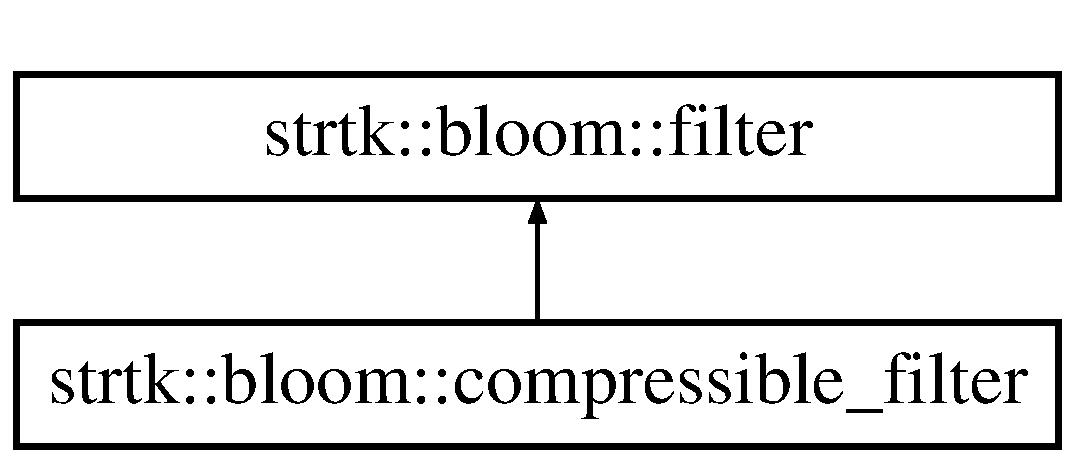
\includegraphics[height=2.000000cm]{classstrtk_1_1bloom_1_1compressible__filter}
\end{center}
\end{figure}
\subsection*{Public Member Functions}
\begin{DoxyCompactItemize}
\item 
\hypertarget{classstrtk_1_1bloom_1_1compressible__filter_a91e789f22f79ccebd6b5cfe74686357a}{{\bfseries compressible\-\_\-filter} (const \hyperlink{classstrtk_1_1bloom_1_1parameters}{parameters} \&p)}\label{classstrtk_1_1bloom_1_1compressible__filter_a91e789f22f79ccebd6b5cfe74686357a}

\item 
\hypertarget{classstrtk_1_1bloom_1_1compressible__filter_aa3f4cf27e089b0cbebd93e041adbcd27}{virtual unsigned long long int {\bfseries size} () const }\label{classstrtk_1_1bloom_1_1compressible__filter_aa3f4cf27e089b0cbebd93e041adbcd27}

\item 
\hypertarget{classstrtk_1_1bloom_1_1compressible__filter_a558c41b3517cf726e2af09571df1aee7}{bool {\bfseries compress} (const double \&percentage)}\label{classstrtk_1_1bloom_1_1compressible__filter_a558c41b3517cf726e2af09571df1aee7}

\end{DoxyCompactItemize}
\subsection*{Additional Inherited Members}


The documentation for this class was generated from the following file\-:\begin{DoxyCompactItemize}
\item 
strtk.\-hpp\end{DoxyCompactItemize}

\hypertarget{classstrtk_1_1details_1_1container__adder}{\section{strtk\-:\-:details\-:\-:container\-\_\-adder Class Reference}
\label{classstrtk_1_1details_1_1container__adder}\index{strtk\-::details\-::container\-\_\-adder@{strtk\-::details\-::container\-\_\-adder}}
}
\subsection*{Public Member Functions}
\begin{DoxyCompactItemize}
\item 
\hypertarget{classstrtk_1_1details_1_1container__adder_a53db8b431a36feeba1e6ffe56b45fa99}{{\footnotesize template$<$typename T , typename Allocator $>$ }\\{\bfseries container\-\_\-adder} (std\-::vector$<$ T, Allocator $>$ \&vec)}\label{classstrtk_1_1details_1_1container__adder_a53db8b431a36feeba1e6ffe56b45fa99}

\item 
\hypertarget{classstrtk_1_1details_1_1container__adder_aa3419a65431adeef1036f1c46d638597}{{\footnotesize template$<$typename T , typename Allocator $>$ }\\{\bfseries container\-\_\-adder} (std\-::deque$<$ T, Allocator $>$ \&deq)}\label{classstrtk_1_1details_1_1container__adder_aa3419a65431adeef1036f1c46d638597}

\item 
\hypertarget{classstrtk_1_1details_1_1container__adder_a9b961cbb6aec9fde7d4f6e47dd96b260}{{\footnotesize template$<$typename T , typename Allocator $>$ }\\{\bfseries container\-\_\-adder} (std\-::list$<$ T, Allocator $>$ \&list)}\label{classstrtk_1_1details_1_1container__adder_a9b961cbb6aec9fde7d4f6e47dd96b260}

\item 
\hypertarget{classstrtk_1_1details_1_1container__adder_a23305833ea58aa9e7fcaae10e81d3dde}{{\footnotesize template$<$typename T , typename Comparator , typename Allocator $>$ }\\{\bfseries container\-\_\-adder} (std\-::set$<$ T, Comparator, Allocator $>$ \&set)}\label{classstrtk_1_1details_1_1container__adder_a23305833ea58aa9e7fcaae10e81d3dde}

\item 
\hypertarget{classstrtk_1_1details_1_1container__adder_aa3f0e628ab1475ac802d1a9d88e51c6c}{{\footnotesize template$<$typename T , typename Comparator , typename Allocator $>$ }\\{\bfseries container\-\_\-adder} (std\-::multiset$<$ T, Comparator, Allocator $>$ \&multiset)}\label{classstrtk_1_1details_1_1container__adder_aa3f0e628ab1475ac802d1a9d88e51c6c}

\item 
\hypertarget{classstrtk_1_1details_1_1container__adder_a068c465f787db3f6de24eb81b6c2e803}{{\footnotesize template$<$typename T , typename Container , typename Comparator $>$ }\\{\bfseries container\-\_\-adder} (std\-::priority\-\_\-queue$<$ T, Container, Comparator $>$ \&pq)}\label{classstrtk_1_1details_1_1container__adder_a068c465f787db3f6de24eb81b6c2e803}

\item 
\hypertarget{classstrtk_1_1details_1_1container__adder_a2226802e2952db90be699f8fa826514a}{{\footnotesize template$<$typename T , typename Container $>$ }\\{\bfseries container\-\_\-adder} (std\-::queue$<$ T, Container $>$ \&queue)}\label{classstrtk_1_1details_1_1container__adder_a2226802e2952db90be699f8fa826514a}

\item 
\hypertarget{classstrtk_1_1details_1_1container__adder_a263bbe26359b3fa928c976f89a3ef299}{{\footnotesize template$<$typename T , typename Container $>$ }\\{\bfseries container\-\_\-adder} (std\-::stack$<$ T, Container $>$ \&stack)}\label{classstrtk_1_1details_1_1container__adder_a263bbe26359b3fa928c976f89a3ef299}

\item 
\hypertarget{classstrtk_1_1details_1_1container__adder_a3256901100af9f1f7a9c648401fa79e1}{{\footnotesize template$<$typename Input\-Iterator $>$ }\\bool {\bfseries add} (Input\-Iterator begin, Input\-Iterator end) const }\label{classstrtk_1_1details_1_1container__adder_a3256901100af9f1f7a9c648401fa79e1}

\item 
\hypertarget{classstrtk_1_1details_1_1container__adder_ac8784f29a4bfd5ff3fa3592dea645860}{{\footnotesize template$<$typename Input\-Iterator $>$ }\\bool {\bfseries add} (std\-::pair$<$ Input\-Iterator, Input\-Iterator $>$ \&range) const }\label{classstrtk_1_1details_1_1container__adder_ac8784f29a4bfd5ff3fa3592dea645860}

\item 
\hypertarget{classstrtk_1_1details_1_1container__adder_afd18fff9a1326a6a826a257e79df2c6f}{{\footnotesize template$<$typename Input\-Iterator $>$ }\\bool {\bfseries operator()} (const Input\-Iterator begin, const Input\-Iterator end)}\label{classstrtk_1_1details_1_1container__adder_afd18fff9a1326a6a826a257e79df2c6f}

\end{DoxyCompactItemize}


The documentation for this class was generated from the following file\-:\begin{DoxyCompactItemize}
\item 
strtk.\-hpp\end{DoxyCompactItemize}

\hypertarget{classstrtk_1_1details_1_1conv__to__lcase__impl}{\section{strtk\-:\-:details\-:\-:conv\-\_\-to\-\_\-lcase\-\_\-impl Class Reference}
\label{classstrtk_1_1details_1_1conv__to__lcase__impl}\index{strtk\-::details\-::conv\-\_\-to\-\_\-lcase\-\_\-impl@{strtk\-::details\-::conv\-\_\-to\-\_\-lcase\-\_\-impl}}
}
\subsection*{Public Member Functions}
\begin{DoxyCompactItemize}
\item 
\hypertarget{classstrtk_1_1details_1_1conv__to__lcase__impl_abcce88a30d104ca130a8465cc5e6b8d0}{{\bfseries conv\-\_\-to\-\_\-lcase\-\_\-impl} (std\-::string \&s)}\label{classstrtk_1_1details_1_1conv__to__lcase__impl_abcce88a30d104ca130a8465cc5e6b8d0}

\item 
\hypertarget{classstrtk_1_1details_1_1conv__to__lcase__impl_adbacc15e95804f1f1cba2d7a9e31e6dc}{{\footnotesize template$<$typename Input\-Iterator $>$ }\\bool {\bfseries operator()} (Input\-Iterator begin, Input\-Iterator end)}\label{classstrtk_1_1details_1_1conv__to__lcase__impl_adbacc15e95804f1f1cba2d7a9e31e6dc}

\item 
\hypertarget{classstrtk_1_1details_1_1conv__to__lcase__impl_a5258aa98175de5fa240e46aff6b253fb}{\hyperlink{classstrtk_1_1details_1_1conv__to__lcase__impl}{conv\-\_\-to\-\_\-lcase\-\_\-impl} \& {\bfseries ref} ()}\label{classstrtk_1_1details_1_1conv__to__lcase__impl_a5258aa98175de5fa240e46aff6b253fb}

\end{DoxyCompactItemize}


The documentation for this class was generated from the following file\-:\begin{DoxyCompactItemize}
\item 
strtk.\-hpp\end{DoxyCompactItemize}

\hypertarget{classstrtk_1_1details_1_1conv__to__ucase__impl}{\section{strtk\-:\-:details\-:\-:conv\-\_\-to\-\_\-ucase\-\_\-impl Class Reference}
\label{classstrtk_1_1details_1_1conv__to__ucase__impl}\index{strtk\-::details\-::conv\-\_\-to\-\_\-ucase\-\_\-impl@{strtk\-::details\-::conv\-\_\-to\-\_\-ucase\-\_\-impl}}
}
\subsection*{Public Member Functions}
\begin{DoxyCompactItemize}
\item 
\hypertarget{classstrtk_1_1details_1_1conv__to__ucase__impl_a33279e829f6cc07c6c47825eb2661050}{{\bfseries conv\-\_\-to\-\_\-ucase\-\_\-impl} (std\-::string \&s)}\label{classstrtk_1_1details_1_1conv__to__ucase__impl_a33279e829f6cc07c6c47825eb2661050}

\item 
\hypertarget{classstrtk_1_1details_1_1conv__to__ucase__impl_aa2d6ddb5ace785712ee834fd2a969ef1}{{\footnotesize template$<$typename Input\-Iterator $>$ }\\bool {\bfseries operator()} (Input\-Iterator begin, Input\-Iterator end)}\label{classstrtk_1_1details_1_1conv__to__ucase__impl_aa2d6ddb5ace785712ee834fd2a969ef1}

\item 
\hypertarget{classstrtk_1_1details_1_1conv__to__ucase__impl_a3407261858895ffc4ab2f72ad2c909b5}{\hyperlink{classstrtk_1_1details_1_1conv__to__ucase__impl}{conv\-\_\-to\-\_\-ucase\-\_\-impl} \& {\bfseries ref} ()}\label{classstrtk_1_1details_1_1conv__to__ucase__impl_a3407261858895ffc4ab2f72ad2c909b5}

\end{DoxyCompactItemize}


The documentation for this class was generated from the following file\-:\begin{DoxyCompactItemize}
\item 
strtk.\-hpp\end{DoxyCompactItemize}

\hypertarget{structstrtk_1_1details_1_1trim__details_1_1convert__impl}{\section{strtk\-:\-:details\-:\-:trim\-\_\-details\-:\-:convert\-\_\-impl$<$ Type $>$ Struct Template Reference}
\label{structstrtk_1_1details_1_1trim__details_1_1convert__impl}\index{strtk\-::details\-::trim\-\_\-details\-::convert\-\_\-impl$<$ Type $>$@{strtk\-::details\-::trim\-\_\-details\-::convert\-\_\-impl$<$ Type $>$}}
}
\subsection*{Static Public Member Functions}
\begin{DoxyCompactItemize}
\item 
\hypertarget{structstrtk_1_1details_1_1trim__details_1_1convert__impl_a9614e3810124241c8db91f6af54335a2}{{\footnotesize template$<$typename Input\-Iterator $>$ }\\static bool {\bfseries execute} (Input\-Iterator begin, Input\-Iterator end, const std\-::string \&rem\-\_\-chars, std\-::size\-\_\-t mode, Type \&t)}\label{structstrtk_1_1details_1_1trim__details_1_1convert__impl_a9614e3810124241c8db91f6af54335a2}

\end{DoxyCompactItemize}


The documentation for this struct was generated from the following file\-:\begin{DoxyCompactItemize}
\item 
strtk.\-hpp\end{DoxyCompactItemize}

\hypertarget{structstrtk_1_1details_1_1trim__details_1_1convert__impl_3_01std_1_1string_01_4}{\section{strtk\-:\-:details\-:\-:trim\-\_\-details\-:\-:convert\-\_\-impl$<$ std\-:\-:string $>$ Struct Template Reference}
\label{structstrtk_1_1details_1_1trim__details_1_1convert__impl_3_01std_1_1string_01_4}\index{strtk\-::details\-::trim\-\_\-details\-::convert\-\_\-impl$<$ std\-::string $>$@{strtk\-::details\-::trim\-\_\-details\-::convert\-\_\-impl$<$ std\-::string $>$}}
}
\subsection*{Static Public Member Functions}
\begin{DoxyCompactItemize}
\item 
\hypertarget{structstrtk_1_1details_1_1trim__details_1_1convert__impl_3_01std_1_1string_01_4_ac32f3868e2e2c43c8109635570581bc1}{{\footnotesize template$<$typename Input\-Iterator $>$ }\\static bool {\bfseries execute} (Input\-Iterator begin, Input\-Iterator end, const std\-::string \&rem\-\_\-chars, std\-::size\-\_\-t mode, std\-::string \&t)}\label{structstrtk_1_1details_1_1trim__details_1_1convert__impl_3_01std_1_1string_01_4_ac32f3868e2e2c43c8109635570581bc1}

\end{DoxyCompactItemize}


The documentation for this struct was generated from the following file\-:\begin{DoxyCompactItemize}
\item 
strtk.\-hpp\end{DoxyCompactItemize}

\hypertarget{classstrtk_1_1counting__back__inserter__iterator}{\section{strtk\-:\-:counting\-\_\-back\-\_\-inserter\-\_\-iterator$<$ T $>$ Class Template Reference}
\label{classstrtk_1_1counting__back__inserter__iterator}\index{strtk\-::counting\-\_\-back\-\_\-inserter\-\_\-iterator$<$ T $>$@{strtk\-::counting\-\_\-back\-\_\-inserter\-\_\-iterator$<$ T $>$}}
}
Inheritance diagram for strtk\-:\-:counting\-\_\-back\-\_\-inserter\-\_\-iterator$<$ T $>$\-:\begin{figure}[H]
\begin{center}
\leavevmode
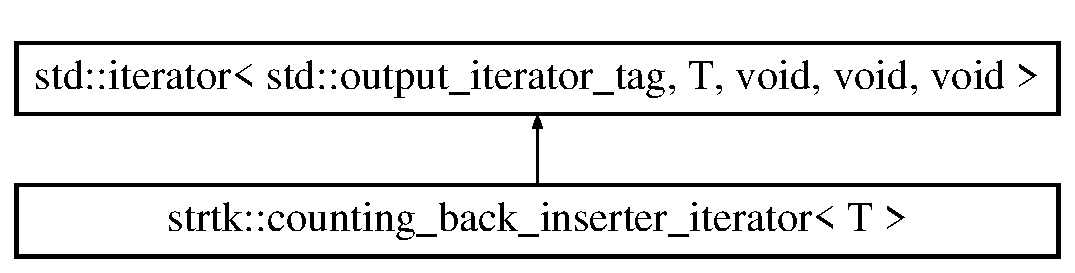
\includegraphics[height=2.000000cm]{classstrtk_1_1counting__back__inserter__iterator}
\end{center}
\end{figure}
\subsection*{Public Member Functions}
\begin{DoxyCompactItemize}
\item 
\hypertarget{classstrtk_1_1counting__back__inserter__iterator_a4df285a14db94568615e41201f467777}{{\bfseries counting\-\_\-back\-\_\-inserter\-\_\-iterator} (std\-::size\-\_\-t \&counter)}\label{classstrtk_1_1counting__back__inserter__iterator_a4df285a14db94568615e41201f467777}

\item 
\hypertarget{classstrtk_1_1counting__back__inserter__iterator_abb28251d4c80a93186dbf0367bb78a65}{{\bfseries counting\-\_\-back\-\_\-inserter\-\_\-iterator} (const \hyperlink{classstrtk_1_1counting__back__inserter__iterator}{counting\-\_\-back\-\_\-inserter\-\_\-iterator} \&itr)}\label{classstrtk_1_1counting__back__inserter__iterator_abb28251d4c80a93186dbf0367bb78a65}

\item 
\hypertarget{classstrtk_1_1counting__back__inserter__iterator_a5340c3b04ec8a656b578b3ac7e0ce9fb}{\hyperlink{classstrtk_1_1counting__back__inserter__iterator}{counting\-\_\-back\-\_\-inserter\-\_\-iterator} \& {\bfseries operator=} (const \hyperlink{classstrtk_1_1counting__back__inserter__iterator}{counting\-\_\-back\-\_\-inserter\-\_\-iterator} \&itr)}\label{classstrtk_1_1counting__back__inserter__iterator_a5340c3b04ec8a656b578b3ac7e0ce9fb}

\item 
\hypertarget{classstrtk_1_1counting__back__inserter__iterator_aa7680ffd03f98879227e8e25b53bf586}{\hyperlink{classstrtk_1_1counting__back__inserter__iterator}{counting\-\_\-back\-\_\-inserter\-\_\-iterator} \& {\bfseries operator=} (const T \&)}\label{classstrtk_1_1counting__back__inserter__iterator_aa7680ffd03f98879227e8e25b53bf586}

\item 
\hypertarget{classstrtk_1_1counting__back__inserter__iterator_a02b69e617230b40d8179d3dbd87fc638}{void {\bfseries operator()} (const T \&)}\label{classstrtk_1_1counting__back__inserter__iterator_a02b69e617230b40d8179d3dbd87fc638}

\item 
\hypertarget{classstrtk_1_1counting__back__inserter__iterator_a77078da25b47e7cbb010dac2c7b31d2c}{\hyperlink{classstrtk_1_1counting__back__inserter__iterator}{counting\-\_\-back\-\_\-inserter\-\_\-iterator} \& {\bfseries operator$\ast$} ()}\label{classstrtk_1_1counting__back__inserter__iterator_a77078da25b47e7cbb010dac2c7b31d2c}

\item 
\hypertarget{classstrtk_1_1counting__back__inserter__iterator_a2d7b29c8db98c897ab696805b7a3d107}{\hyperlink{classstrtk_1_1counting__back__inserter__iterator}{counting\-\_\-back\-\_\-inserter\-\_\-iterator} \& {\bfseries operator++} ()}\label{classstrtk_1_1counting__back__inserter__iterator_a2d7b29c8db98c897ab696805b7a3d107}

\item 
\hypertarget{classstrtk_1_1counting__back__inserter__iterator_a2428a4e887900465aea1d5c63c7b55d3}{\hyperlink{classstrtk_1_1counting__back__inserter__iterator}{counting\-\_\-back\-\_\-inserter\-\_\-iterator} {\bfseries operator++} (int)}\label{classstrtk_1_1counting__back__inserter__iterator_a2428a4e887900465aea1d5c63c7b55d3}

\end{DoxyCompactItemize}


The documentation for this class was generated from the following file\-:\begin{DoxyCompactItemize}
\item 
strtk.\-hpp\end{DoxyCompactItemize}

\hypertarget{classstrtk_1_1decimal__sink}{\section{strtk\-:\-:decimal\-\_\-sink$<$ T $>$ Class Template Reference}
\label{classstrtk_1_1decimal__sink}\index{strtk\-::decimal\-\_\-sink$<$ T $>$@{strtk\-::decimal\-\_\-sink$<$ T $>$}}
}
\subsection*{Public Member Functions}
\begin{DoxyCompactItemize}
\item 
\hypertarget{classstrtk_1_1decimal__sink_ac6977089427d56b187cfc43e1ec55b86}{{\bfseries decimal\-\_\-sink} (const std\-::size\-\_\-t \&int\-\_\-size, const std\-::size\-\_\-t \&frac\-\_\-size)}\label{classstrtk_1_1decimal__sink_ac6977089427d56b187cfc43e1ec55b86}

\item 
\hypertarget{classstrtk_1_1decimal__sink_aabb28e47b7ab7a734b00730ec1323b3b}{{\bfseries decimal\-\_\-sink} (T \&t, const std\-::size\-\_\-t \&int\-\_\-size, const std\-::size\-\_\-t \&frac\-\_\-size)}\label{classstrtk_1_1decimal__sink_aabb28e47b7ab7a734b00730ec1323b3b}

\item 
\hypertarget{classstrtk_1_1decimal__sink_aa262b81fa09e3fc8d0684b8963e40a93}{\hyperlink{classstrtk_1_1decimal__sink}{decimal\-\_\-sink} \& {\bfseries int\-\_\-size} (const std\-::size\-\_\-t \&size)}\label{classstrtk_1_1decimal__sink_aa262b81fa09e3fc8d0684b8963e40a93}

\item 
\hypertarget{classstrtk_1_1decimal__sink_a2fd63539f191ba2dd7b288de2a89b235}{\hyperlink{classstrtk_1_1decimal__sink}{decimal\-\_\-sink} \& {\bfseries frac\-\_\-size} (const std\-::size\-\_\-t \&size)}\label{classstrtk_1_1decimal__sink_a2fd63539f191ba2dd7b288de2a89b235}

\item 
\hypertarget{classstrtk_1_1decimal__sink_a3ed3ea8c3bf6993487da01bb66816563}{\hyperlink{classstrtk_1_1decimal__sink}{decimal\-\_\-sink} \& {\bfseries operator()} (T \&t)}\label{classstrtk_1_1decimal__sink_a3ed3ea8c3bf6993487da01bb66816563}

\item 
\hypertarget{classstrtk_1_1decimal__sink_a74b16e8e3f359d707298328a07e27c28}{{\footnotesize template$<$typename Input\-Iterator $>$ }\\bool {\bfseries operator()} (Input\-Iterator itr, Input\-Iterator end)}\label{classstrtk_1_1decimal__sink_a74b16e8e3f359d707298328a07e27c28}

\end{DoxyCompactItemize}


The documentation for this class was generated from the following file\-:\begin{DoxyCompactItemize}
\item 
strtk.\-hpp\end{DoxyCompactItemize}

\hypertarget{structstrtk_1_1details_1_1decsink__type__tag}{\section{strtk\-:\-:details\-:\-:decsink\-\_\-type\-\_\-tag Struct Reference}
\label{structstrtk_1_1details_1_1decsink__type__tag}\index{strtk\-::details\-::decsink\-\_\-type\-\_\-tag@{strtk\-::details\-::decsink\-\_\-type\-\_\-tag}}
}


The documentation for this struct was generated from the following file\-:\begin{DoxyCompactItemize}
\item 
strtk.\-hpp\end{DoxyCompactItemize}

\hypertarget{structstrtk_1_1deque__sink}{\section{strtk\-:\-:deque\-\_\-sink$<$ T $>$ Struct Template Reference}
\label{structstrtk_1_1deque__sink}\index{strtk\-::deque\-\_\-sink$<$ T $>$@{strtk\-::deque\-\_\-sink$<$ T $>$}}
}
\subsection*{Public Types}
\begin{DoxyCompactItemize}
\item 
\hypertarget{structstrtk_1_1deque__sink_a49184fb04ab829b6b2ada53c11b05551}{typedef \hyperlink{classstrtk_1_1sink__type}{sink\-\_\-type}$<$ std\-::deque\\*
$<$ T $>$ $>$ {\bfseries type}}\label{structstrtk_1_1deque__sink_a49184fb04ab829b6b2ada53c11b05551}

\end{DoxyCompactItemize}


The documentation for this struct was generated from the following file\-:\begin{DoxyCompactItemize}
\item 
strtk.\-hpp\end{DoxyCompactItemize}

\hypertarget{classDictionary}{\section{Dictionary Class Reference}
\label{classDictionary}\index{Dictionary@{Dictionary}}
}
\subsection*{Public Member Functions}
\begin{DoxyCompactItemize}
\item 
\hypertarget{classDictionary_a590d3076095b179aa1aeb4c8d22234ff}{\hyperlink{classresults}{results} $\ast$ {\bfseries query} (string)}\label{classDictionary_a590d3076095b179aa1aeb4c8d22234ff}

\item 
\hypertarget{classDictionary_a3106fd2d9a299614602bf2f424984de0}{void {\bfseries add\-Word} (string name, string uuid)}\label{classDictionary_a3106fd2d9a299614602bf2f424984de0}

\item 
\hypertarget{classDictionary_a7fe3bb93d4e644f787b1d14f247131c2}{{\bfseries Dictionary} (bool avl)}\label{classDictionary_a7fe3bb93d4e644f787b1d14f247131c2}

\item 
\hypertarget{classDictionary_a67684a55693cc41573d3adbda4929b6a}{void {\bfseries insert} (string n, string u)}\label{classDictionary_a67684a55693cc41573d3adbda4929b6a}

\item 
\hypertarget{classDictionary_a533556e6be15decdc06207bad3ad03c1}{void {\bfseries calc\-Freq} ()}\label{classDictionary_a533556e6be15decdc06207bad3ad03c1}

\end{DoxyCompactItemize}


The documentation for this class was generated from the following files\-:\begin{DoxyCompactItemize}
\item 
dictionary.\-h\item 
dictionary.\-cpp\end{DoxyCompactItemize}

\hypertarget{structstrtk_1_1empty__range}{\section{strtk\-:\-:empty\-\_\-range Struct Reference}
\label{structstrtk_1_1empty__range}\index{strtk\-::empty\-\_\-range@{strtk\-::empty\-\_\-range}}
}
\subsection*{Public Member Functions}
\begin{DoxyCompactItemize}
\item 
\hypertarget{structstrtk_1_1empty__range_a7baa0d630a83b22ccc5f0cafb01dd3cb}{{\footnotesize template$<$typename Input\-Iterator $>$ }\\bool {\bfseries operator()} (const Input\-Iterator begin, const Input\-Iterator end)}\label{structstrtk_1_1empty__range_a7baa0d630a83b22ccc5f0cafb01dd3cb}

\end{DoxyCompactItemize}


The documentation for this struct was generated from the following file\-:\begin{DoxyCompactItemize}
\item 
strtk.\-hpp\end{DoxyCompactItemize}

\hypertarget{structstrtk_1_1details_1_1enable__if}{\section{strtk\-:\-:details\-:\-:enable\-\_\-if$<$ bool, T $>$ Struct Template Reference}
\label{structstrtk_1_1details_1_1enable__if}\index{strtk\-::details\-::enable\-\_\-if$<$ bool, T $>$@{strtk\-::details\-::enable\-\_\-if$<$ bool, T $>$}}
}


The documentation for this struct was generated from the following file\-:\begin{DoxyCompactItemize}
\item 
strtk.\-hpp\end{DoxyCompactItemize}

\hypertarget{structstrtk_1_1details_1_1enable__if_3_01true_00_01T_01_4}{\section{strtk\-:\-:details\-:\-:enable\-\_\-if$<$ true, T $>$ Struct Template Reference}
\label{structstrtk_1_1details_1_1enable__if_3_01true_00_01T_01_4}\index{strtk\-::details\-::enable\-\_\-if$<$ true, T $>$@{strtk\-::details\-::enable\-\_\-if$<$ true, T $>$}}
}
\subsection*{Public Types}
\begin{DoxyCompactItemize}
\item 
\hypertarget{structstrtk_1_1details_1_1enable__if_3_01true_00_01T_01_4_aad3787a57c2c6c8ef4a051801a69ec82}{typedef T {\bfseries type}}\label{structstrtk_1_1details_1_1enable__if_3_01true_00_01T_01_4_aad3787a57c2c6c8ef4a051801a69ec82}

\end{DoxyCompactItemize}


The documentation for this struct was generated from the following file\-:\begin{DoxyCompactItemize}
\item 
strtk.\-hpp\end{DoxyCompactItemize}

\hypertarget{classstrtk_1_1details_1_1expect__impl}{\section{strtk\-:\-:details\-:\-:expect\-\_\-impl Class Reference}
\label{classstrtk_1_1details_1_1expect__impl}\index{strtk\-::details\-::expect\-\_\-impl@{strtk\-::details\-::expect\-\_\-impl}}
}
\subsection*{Public Member Functions}
\begin{DoxyCompactItemize}
\item 
\hypertarget{classstrtk_1_1details_1_1expect__impl_a8902934f4f807b04437290520f7253a3}{{\bfseries expect\-\_\-impl} (const std\-::string \&s)}\label{classstrtk_1_1details_1_1expect__impl_a8902934f4f807b04437290520f7253a3}

\item 
\hypertarget{classstrtk_1_1details_1_1expect__impl_a1496b3d105a07b82055ee81ca70e7772}{{\footnotesize template$<$typename Input\-Iterator $>$ }\\bool {\bfseries operator()} (Input\-Iterator begin, Input\-Iterator end)}\label{classstrtk_1_1details_1_1expect__impl_a1496b3d105a07b82055ee81ca70e7772}

\item 
\hypertarget{classstrtk_1_1details_1_1expect__impl_aa1bd270988a87d7f5b4a3e1f94e426cd}{\hyperlink{classstrtk_1_1details_1_1expect__impl}{expect\-\_\-impl} \& {\bfseries ref} ()}\label{classstrtk_1_1details_1_1expect__impl_aa1bd270988a87d7f5b4a3e1f94e426cd}

\item 
\hypertarget{classstrtk_1_1details_1_1expect__impl_abd7d7f9595bba5a9be009516de67cc23}{void {\bfseries set\-\_\-value} (const std\-::string \&s)}\label{classstrtk_1_1details_1_1expect__impl_abd7d7f9595bba5a9be009516de67cc23}

\end{DoxyCompactItemize}


The documentation for this class was generated from the following file\-:\begin{DoxyCompactItemize}
\item 
strtk.\-hpp\end{DoxyCompactItemize}

\hypertarget{structstrtk_1_1details_1_1expect__type__tag}{\section{strtk\-:\-:details\-:\-:expect\-\_\-type\-\_\-tag Struct Reference}
\label{structstrtk_1_1details_1_1expect__type__tag}\index{strtk\-::details\-::expect\-\_\-type\-\_\-tag@{strtk\-::details\-::expect\-\_\-type\-\_\-tag}}
}


The documentation for this struct was generated from the following file\-:\begin{DoxyCompactItemize}
\item 
strtk.\-hpp\end{DoxyCompactItemize}

\hypertarget{classstrtk_1_1ext__string}{\section{strtk\-:\-:ext\-\_\-string Class Reference}
\label{classstrtk_1_1ext__string}\index{strtk\-::ext\-\_\-string@{strtk\-::ext\-\_\-string}}
}
\subsection*{Public Member Functions}
\begin{DoxyCompactItemize}
\item 
\hypertarget{classstrtk_1_1ext__string_a2e2b1988c50b76862b947a18e81f8598}{{\bfseries ext\-\_\-string} (const std\-::string \&s)}\label{classstrtk_1_1ext__string_a2e2b1988c50b76862b947a18e81f8598}

\item 
\hypertarget{classstrtk_1_1ext__string_aac355036aae1df3b11ea73ac6e677672}{{\bfseries ext\-\_\-string} (const char $\ast$s)}\label{classstrtk_1_1ext__string_aac355036aae1df3b11ea73ac6e677672}

\item 
\hypertarget{classstrtk_1_1ext__string_aa8e59978f18beb48b5bc8fe0ea2aa92b}{{\bfseries ext\-\_\-string} (const \hyperlink{classstrtk_1_1range_1_1adapter}{range\-::adapter}$<$ char $>$ \&r)}\label{classstrtk_1_1ext__string_aa8e59978f18beb48b5bc8fe0ea2aa92b}

\item 
\hypertarget{classstrtk_1_1ext__string_a34d67e0b4682c6a6e36064a621d27d71}{{\bfseries ext\-\_\-string} (const \hyperlink{classstrtk_1_1ext__string}{ext\-\_\-string} \&es)}\label{classstrtk_1_1ext__string_a34d67e0b4682c6a6e36064a621d27d71}

\item 
\hypertarget{classstrtk_1_1ext__string_addc4c0645e2997ee70795d2b772a8252}{{\footnotesize template$<$typename T $>$ }\\\hyperlink{classstrtk_1_1ext__string}{ext\-\_\-string} \& {\bfseries operator$<$$<$} (const T \&t)}\label{classstrtk_1_1ext__string_addc4c0645e2997ee70795d2b772a8252}

\item 
\hypertarget{classstrtk_1_1ext__string_a9b8a727de635835be44d15cd2461017e}{{\bfseries operator std\-::string} () const }\label{classstrtk_1_1ext__string_a9b8a727de635835be44d15cd2461017e}

\item 
\hypertarget{classstrtk_1_1ext__string_a986ffd65d26af6b32e97ee3d416c4397}{std\-::string {\bfseries clone} () const }\label{classstrtk_1_1ext__string_a986ffd65d26af6b32e97ee3d416c4397}

\item 
\hypertarget{classstrtk_1_1ext__string_ae7eb1b304c5e2bf1f7fa12c40ab06d88}{const std\-::string \& {\bfseries as\-\_\-string} () const }\label{classstrtk_1_1ext__string_ae7eb1b304c5e2bf1f7fa12c40ab06d88}

\item 
\hypertarget{classstrtk_1_1ext__string_a7cd3caaa8b603e2f8e3b03417b50376a}{std\-::string \& {\bfseries as\-\_\-string} ()}\label{classstrtk_1_1ext__string_a7cd3caaa8b603e2f8e3b03417b50376a}

\item 
\hypertarget{classstrtk_1_1ext__string_adced43a1cf8105d7046fcae82758840c}{{\footnotesize template$<$typename T $>$ }\\T {\bfseries as\-\_\-type} () const }\label{classstrtk_1_1ext__string_adced43a1cf8105d7046fcae82758840c}

\item 
\hypertarget{classstrtk_1_1ext__string_a38ac5f330d997629ce9e78edd1fc3aaf}{{\footnotesize template$<$typename T $>$ }\\bool {\bfseries as\-\_\-type} (T \&t) const }\label{classstrtk_1_1ext__string_a38ac5f330d997629ce9e78edd1fc3aaf}

\item 
\hypertarget{classstrtk_1_1ext__string_af8f018508c982b850dab5bed14e0c568}{bool {\bfseries imatch} (const std\-::string \&s) const }\label{classstrtk_1_1ext__string_af8f018508c982b850dab5bed14e0c568}

\item 
\hypertarget{classstrtk_1_1ext__string_a9e0678312a91f8c73636b7c56661235a}{bool {\bfseries imatch} (const \hyperlink{classstrtk_1_1ext__string}{ext\-\_\-string} \&es) const }\label{classstrtk_1_1ext__string_a9e0678312a91f8c73636b7c56661235a}

\item 
\hypertarget{classstrtk_1_1ext__string_a23574829824c5fe72e489ee8997b0dd7}{\hyperlink{classstrtk_1_1ext__string}{ext\-\_\-string} \& {\bfseries to\-\_\-lowercase} ()}\label{classstrtk_1_1ext__string_a23574829824c5fe72e489ee8997b0dd7}

\item 
\hypertarget{classstrtk_1_1ext__string_a0a96f389dd613c9d062d417897dc1365}{\hyperlink{classstrtk_1_1ext__string}{ext\-\_\-string} \& {\bfseries to\-\_\-uppercase} ()}\label{classstrtk_1_1ext__string_a0a96f389dd613c9d062d417897dc1365}

\item 
\hypertarget{classstrtk_1_1ext__string_a451346adf33e950642197827bb11621b}{{\footnotesize template$<$typename Predicate $>$ }\\\hyperlink{classstrtk_1_1ext__string}{ext\-\_\-string} \& {\bfseries remove\-\_\-leading} (const Predicate \&p)}\label{classstrtk_1_1ext__string_a451346adf33e950642197827bb11621b}

\item 
\hypertarget{classstrtk_1_1ext__string_aa1008ba0bc73714350da5440eecb37c2}{\hyperlink{classstrtk_1_1ext__string}{ext\-\_\-string} \& {\bfseries remove\-\_\-leading} (const std\-::string \&removal\-\_\-set)}\label{classstrtk_1_1ext__string_aa1008ba0bc73714350da5440eecb37c2}

\item 
\hypertarget{classstrtk_1_1ext__string_a079cda4fdd3d5904538346978c63222a}{{\footnotesize template$<$typename Predicate $>$ }\\\hyperlink{classstrtk_1_1ext__string}{ext\-\_\-string} \& {\bfseries remove\-\_\-trailing} (const Predicate \&p)}\label{classstrtk_1_1ext__string_a079cda4fdd3d5904538346978c63222a}

\item 
\hypertarget{classstrtk_1_1ext__string_aa6d7f67d5ccd9abd724a5972c34f0581}{\hyperlink{classstrtk_1_1ext__string}{ext\-\_\-string} \& {\bfseries remove\-\_\-trailing} (const std\-::string \&removal\-\_\-set)}\label{classstrtk_1_1ext__string_aa6d7f67d5ccd9abd724a5972c34f0581}

\item 
\hypertarget{classstrtk_1_1ext__string_ab2aed17b629f9ce5a6be6f2885a48de9}{{\footnotesize template$<$typename T $>$ }\\\hyperlink{classstrtk_1_1ext__string}{ext\-\_\-string} \& {\bfseries operator+=} (const T \&t)}\label{classstrtk_1_1ext__string_ab2aed17b629f9ce5a6be6f2885a48de9}

\item 
\hypertarget{classstrtk_1_1ext__string_a9d98afbdfc3947ee99dbb80835bb4600}{\hyperlink{classstrtk_1_1ext__string}{ext\-\_\-string} \& {\bfseries operator-\/=} (const std\-::string \&pattern)}\label{classstrtk_1_1ext__string_a9d98afbdfc3947ee99dbb80835bb4600}

\item 
\hypertarget{classstrtk_1_1ext__string_a87739d8e2f948c47d01ea073984b0e00}{\hyperlink{classstrtk_1_1ext__string}{ext\-\_\-string} \& {\bfseries operator$\ast$=} (const std\-::size\-\_\-t \&n)}\label{classstrtk_1_1ext__string_a87739d8e2f948c47d01ea073984b0e00}

\item 
\hypertarget{classstrtk_1_1ext__string_a744598abb8c6def7ad303fe7e8edc508}{void {\bfseries replace} (const std\-::string \&pattern, const std\-::string \&replace\-\_\-pattern)}\label{classstrtk_1_1ext__string_a744598abb8c6def7ad303fe7e8edc508}

\item 
\hypertarget{classstrtk_1_1ext__string_afd2ad93313e0c3f2845c4679b688ff7c}{{\footnotesize template$<$typename Delimiter\-Predicate , typename Output\-Iterator $>$ }\\std\-::size\-\_\-t {\bfseries split} (const Delimiter\-Predicate \&p, Output\-Iterator out, const split\-\_\-options\-::type split\-\_\-option=split\-\_\-options\-::default\-\_\-mode) const }\label{classstrtk_1_1ext__string_afd2ad93313e0c3f2845c4679b688ff7c}

\item 
\hypertarget{classstrtk_1_1ext__string_a5bbc5261cb10147acda8925430719cee}{{\footnotesize template$<$typename Delimiter\-Predicate , typename Allocator , template$<$ typename, typename $>$ class Sequence$>$ }\\std\-::size\-\_\-t {\bfseries split} (const Delimiter\-Predicate \&p, Sequence$<$ std\-::string, Allocator $>$ \&seq, const split\-\_\-options\-::type split\-\_\-option=split\-\_\-options\-::default\-\_\-mode) const }\label{classstrtk_1_1ext__string_a5bbc5261cb10147acda8925430719cee}

\item 
\hypertarget{classstrtk_1_1ext__string_abdfd7eaef30588874a8e9be2248ec462}{{\footnotesize template$<$typename Delimiter\-Predicate , typename Output\-Iterator $>$ }\\std\-::size\-\_\-t {\bfseries split\-\_\-n} (const Delimiter\-Predicate \&p, const std\-::size\-\_\-t \&n, Output\-Iterator out, const split\-\_\-options\-::type split\-\_\-option=split\-\_\-options\-::default\-\_\-mode) const }\label{classstrtk_1_1ext__string_abdfd7eaef30588874a8e9be2248ec462}

\item 
\hypertarget{classstrtk_1_1ext__string_aaec150c9d2dfdc87d02d40857df6c4a5}{{\footnotesize template$<$typename Delimiter\-Predicate , typename Allocator , template$<$ typename, typename $>$ class Sequence$>$ }\\std\-::size\-\_\-t {\bfseries split\-\_\-n} (const Delimiter\-Predicate \&p, const std\-::size\-\_\-t \&n, Sequence$<$ std\-::string, Allocator $>$ \&seq, const split\-\_\-options\-::type split\-\_\-option=split\-\_\-options\-::default\-\_\-mode) const }\label{classstrtk_1_1ext__string_aaec150c9d2dfdc87d02d40857df6c4a5}

\item 
\hypertarget{classstrtk_1_1ext__string_a5fa9c21c7ecd64b4b3da5c3396af0b51}{{\footnotesize template$<$typename T , typename Allocator , template$<$ typename, typename $>$ class Sequence$>$ }\\std\-::size\-\_\-t {\bfseries parse} (const std\-::string \&delimiters, Sequence$<$ T, Allocator $>$ \&seq) const }\label{classstrtk_1_1ext__string_a5fa9c21c7ecd64b4b3da5c3396af0b51}

\item 
\hypertarget{classstrtk_1_1ext__string_ab017dc85c08135189d1a40240bb022b4}{{\footnotesize template$<$typename T , typename Allocator , template$<$ typename, typename $>$ class Sequence$>$ }\\std\-::size\-\_\-t {\bfseries parse} (const char $\ast$delimiters, Sequence$<$ T, Allocator $>$ \&seq) const }\label{classstrtk_1_1ext__string_ab017dc85c08135189d1a40240bb022b4}

\end{DoxyCompactItemize}
\subsection*{Static Public Member Functions}
\begin{DoxyCompactItemize}
\item 
\hypertarget{classstrtk_1_1ext__string_a8a219b9138f11bbae3e8dce696676de2}{static \hyperlink{classstrtk_1_1ext__string}{ext\-\_\-string} {\bfseries all\-\_\-digits} ()}\label{classstrtk_1_1ext__string_a8a219b9138f11bbae3e8dce696676de2}

\item 
\hypertarget{classstrtk_1_1ext__string_a1fcfcfb44b6ea63449a6791b53c6a455}{static \hyperlink{classstrtk_1_1ext__string}{ext\-\_\-string} {\bfseries all\-\_\-letters} ()}\label{classstrtk_1_1ext__string_a1fcfcfb44b6ea63449a6791b53c6a455}

\item 
\hypertarget{classstrtk_1_1ext__string_ac8cd09014f4be0a655aa036e455eef12}{static \hyperlink{classstrtk_1_1ext__string}{ext\-\_\-string} {\bfseries all\-\_\-lowercase\-\_\-letters} ()}\label{classstrtk_1_1ext__string_ac8cd09014f4be0a655aa036e455eef12}

\item 
\hypertarget{classstrtk_1_1ext__string_ab58ebb5fd1a442a5119095de35c6b86f}{static \hyperlink{classstrtk_1_1ext__string}{ext\-\_\-string} {\bfseries all\-\_\-uppercase\-\_\-letters} ()}\label{classstrtk_1_1ext__string_ab58ebb5fd1a442a5119095de35c6b86f}

\item 
\hypertarget{classstrtk_1_1ext__string_a598f8cd0af2e6ce0578d92d4e216b312}{static \hyperlink{classstrtk_1_1ext__string}{ext\-\_\-string} {\bfseries all\-\_\-chars} ()}\label{classstrtk_1_1ext__string_a598f8cd0af2e6ce0578d92d4e216b312}

\end{DoxyCompactItemize}
\subsection*{Friends}
\begin{DoxyCompactItemize}
\item 
\hypertarget{classstrtk_1_1ext__string_ae45d367a03f4402e93e819e84253bfaf}{\hyperlink{classstrtk_1_1ext__string}{ext\-\_\-string} {\bfseries operator$\ast$} (const std\-::size\-\_\-t \&n, const \hyperlink{classstrtk_1_1ext__string}{ext\-\_\-string} \&s)}\label{classstrtk_1_1ext__string_ae45d367a03f4402e93e819e84253bfaf}

\item 
\hypertarget{classstrtk_1_1ext__string_a0805d5292ded76de84789c2981eab929}{\hyperlink{classstrtk_1_1ext__string}{ext\-\_\-string} {\bfseries operator$\ast$} (const \hyperlink{classstrtk_1_1ext__string}{ext\-\_\-string} \&s, const std\-::size\-\_\-t \&n)}\label{classstrtk_1_1ext__string_a0805d5292ded76de84789c2981eab929}

\item 
\hypertarget{classstrtk_1_1ext__string_acc1a45ebc03198dd0ad7e3ae17b35172}{{\footnotesize template$<$typename T $>$ }\\\hyperlink{classstrtk_1_1ext__string}{ext\-\_\-string} {\bfseries operator+} (const \hyperlink{classstrtk_1_1ext__string}{ext\-\_\-string} \&s, const T \&t)}\label{classstrtk_1_1ext__string_acc1a45ebc03198dd0ad7e3ae17b35172}

\item 
\hypertarget{classstrtk_1_1ext__string_a9c08b0a72c1209ada8211cc49bf39af4}{{\footnotesize template$<$typename T $>$ }\\\hyperlink{classstrtk_1_1ext__string}{ext\-\_\-string} {\bfseries operator+} (const T \&t, const \hyperlink{classstrtk_1_1ext__string}{ext\-\_\-string} \&s)}\label{classstrtk_1_1ext__string_a9c08b0a72c1209ada8211cc49bf39af4}

\item 
\hypertarget{classstrtk_1_1ext__string_ac10dd5a61ce73046ddcd9b1a50e6eb45}{\hyperlink{classstrtk_1_1ext__string}{ext\-\_\-string} {\bfseries operator-\/} (const \hyperlink{classstrtk_1_1ext__string}{ext\-\_\-string} \&s, const std\-::string \&pattern)}\label{classstrtk_1_1ext__string_ac10dd5a61ce73046ddcd9b1a50e6eb45}

\item 
\hypertarget{classstrtk_1_1ext__string_a7b7096018804ac09008c5a2198a1aa15}{\hyperlink{classstrtk_1_1ext__string}{ext\-\_\-string} {\bfseries operator-\/} (const \hyperlink{classstrtk_1_1ext__string}{ext\-\_\-string} \&s, const char $\ast$pattern)}\label{classstrtk_1_1ext__string_a7b7096018804ac09008c5a2198a1aa15}

\item 
\hypertarget{classstrtk_1_1ext__string_a5ef7087ec839638128fbde61d4821742}{\hyperlink{classstrtk_1_1ext__string}{ext\-\_\-string} {\bfseries operator-\/} (const \hyperlink{classstrtk_1_1ext__string}{ext\-\_\-string} \&s, const \hyperlink{classstrtk_1_1ext__string}{ext\-\_\-string} \&pattern)}\label{classstrtk_1_1ext__string_a5ef7087ec839638128fbde61d4821742}

\end{DoxyCompactItemize}


The documentation for this class was generated from the following file\-:\begin{DoxyCompactItemize}
\item 
strtk.\-hpp\end{DoxyCompactItemize}

\hypertarget{classrapidxml_1_1file}{\section{rapidxml\-:\-:file$<$ Ch $>$ Class Template Reference}
\label{classrapidxml_1_1file}\index{rapidxml\-::file$<$ Ch $>$@{rapidxml\-::file$<$ Ch $>$}}
}


Represents data loaded from a file.  




{\ttfamily \#include $<$rapidxml\-\_\-utils.\-hpp$>$}

\subsection*{Public Member Functions}
\begin{DoxyCompactItemize}
\item 
\hyperlink{classrapidxml_1_1file_ae881a3cab1fe7152d45c92a8d7606cb3}{file} (const char $\ast$filename)
\item 
\hyperlink{classrapidxml_1_1file_a90707ccd991cc392dcf4bef37eed9d1f}{file} (std\-::basic\-\_\-istream$<$ Ch $>$ \&stream)
\item 
Ch $\ast$ \hyperlink{classrapidxml_1_1file_af1c71d65862c7af14e4708e32a80c1de}{data} ()
\item 
const Ch $\ast$ \hyperlink{classrapidxml_1_1file_aceb8f5ebd577c946a74b1ea3e2e0c576}{data} () const 
\item 
std\-::size\-\_\-t \hyperlink{classrapidxml_1_1file_a20191d167c6e00a88a44ca9a3a54e1c5}{size} () const 
\end{DoxyCompactItemize}


\subsection{Detailed Description}
\subsubsection*{template$<$class Ch = char$>$class rapidxml\-::file$<$ Ch $>$}

Represents data loaded from a file. 

\subsection{Constructor \& Destructor Documentation}
\hypertarget{classrapidxml_1_1file_ae881a3cab1fe7152d45c92a8d7606cb3}{\index{rapidxml\-::file@{rapidxml\-::file}!file@{file}}
\index{file@{file}!rapidxml::file@{rapidxml\-::file}}
\subsubsection[{file}]{\setlength{\rightskip}{0pt plus 5cm}template$<$class Ch  = char$>$ {\bf rapidxml\-::file}$<$ Ch $>$\-::{\bf file} (
\begin{DoxyParamCaption}
\item[{const char $\ast$}]{filename}
\end{DoxyParamCaption}
)\hspace{0.3cm}{\ttfamily [inline]}}}\label{classrapidxml_1_1file_ae881a3cab1fe7152d45c92a8d7606cb3}
Loads file into the memory. Data will be automatically destroyed by the destructor. 
\begin{DoxyParams}{Parameters}
{\em filename} & Filename to load. \\
\hline
\end{DoxyParams}
\hypertarget{classrapidxml_1_1file_a90707ccd991cc392dcf4bef37eed9d1f}{\index{rapidxml\-::file@{rapidxml\-::file}!file@{file}}
\index{file@{file}!rapidxml::file@{rapidxml\-::file}}
\subsubsection[{file}]{\setlength{\rightskip}{0pt plus 5cm}template$<$class Ch  = char$>$ {\bf rapidxml\-::file}$<$ Ch $>$\-::{\bf file} (
\begin{DoxyParamCaption}
\item[{std\-::basic\-\_\-istream$<$ Ch $>$ \&}]{stream}
\end{DoxyParamCaption}
)\hspace{0.3cm}{\ttfamily [inline]}}}\label{classrapidxml_1_1file_a90707ccd991cc392dcf4bef37eed9d1f}
Loads file into the memory. Data will be automatically destroyed by the destructor 
\begin{DoxyParams}{Parameters}
{\em stream} & Stream to load from \\
\hline
\end{DoxyParams}


\subsection{Member Function Documentation}
\hypertarget{classrapidxml_1_1file_af1c71d65862c7af14e4708e32a80c1de}{\index{rapidxml\-::file@{rapidxml\-::file}!data@{data}}
\index{data@{data}!rapidxml::file@{rapidxml\-::file}}
\subsubsection[{data}]{\setlength{\rightskip}{0pt plus 5cm}template$<$class Ch  = char$>$ Ch$\ast$ {\bf rapidxml\-::file}$<$ Ch $>$\-::data (
\begin{DoxyParamCaption}
{}
\end{DoxyParamCaption}
)\hspace{0.3cm}{\ttfamily [inline]}}}\label{classrapidxml_1_1file_af1c71d65862c7af14e4708e32a80c1de}
Gets file data. \begin{DoxyReturn}{Returns}
Pointer to data of file. 
\end{DoxyReturn}
\hypertarget{classrapidxml_1_1file_aceb8f5ebd577c946a74b1ea3e2e0c576}{\index{rapidxml\-::file@{rapidxml\-::file}!data@{data}}
\index{data@{data}!rapidxml::file@{rapidxml\-::file}}
\subsubsection[{data}]{\setlength{\rightskip}{0pt plus 5cm}template$<$class Ch  = char$>$ const Ch$\ast$ {\bf rapidxml\-::file}$<$ Ch $>$\-::data (
\begin{DoxyParamCaption}
{}
\end{DoxyParamCaption}
) const\hspace{0.3cm}{\ttfamily [inline]}}}\label{classrapidxml_1_1file_aceb8f5ebd577c946a74b1ea3e2e0c576}
Gets file data. \begin{DoxyReturn}{Returns}
Pointer to data of file. 
\end{DoxyReturn}
\hypertarget{classrapidxml_1_1file_a20191d167c6e00a88a44ca9a3a54e1c5}{\index{rapidxml\-::file@{rapidxml\-::file}!size@{size}}
\index{size@{size}!rapidxml::file@{rapidxml\-::file}}
\subsubsection[{size}]{\setlength{\rightskip}{0pt plus 5cm}template$<$class Ch  = char$>$ std\-::size\-\_\-t {\bf rapidxml\-::file}$<$ Ch $>$\-::size (
\begin{DoxyParamCaption}
{}
\end{DoxyParamCaption}
) const\hspace{0.3cm}{\ttfamily [inline]}}}\label{classrapidxml_1_1file_a20191d167c6e00a88a44ca9a3a54e1c5}
Gets file data size. \begin{DoxyReturn}{Returns}
Size of file data, in characters. 
\end{DoxyReturn}


The documentation for this class was generated from the following file\-:\begin{DoxyCompactItemize}
\item 
\hyperlink{rapidxml__utils_8hpp}{rapidxml\-\_\-utils.\-hpp}\end{DoxyCompactItemize}

\hypertarget{classFileRecord}{\section{File\-Record Class Reference}
\label{classFileRecord}\index{File\-Record@{File\-Record}}
}
\subsection*{Public Member Functions}
\begin{DoxyCompactItemize}
\item 
\hypertarget{classFileRecord_a1fd39e086d42b1221436b697674586c3}{{\bfseries File\-Record} (string fid, long occ)}\label{classFileRecord_a1fd39e086d42b1221436b697674586c3}

\item 
\hypertarget{classFileRecord_af07a3c89d321c1c28dc182354e68f640}{void {\bfseries increment} ()}\label{classFileRecord_af07a3c89d321c1c28dc182354e68f640}

\item 
\hypertarget{classFileRecord_a84f4a499173ccea140e71db2d86ca26f}{void {\bfseries calc\-Freq} ()}\label{classFileRecord_a84f4a499173ccea140e71db2d86ca26f}

\item 
\hypertarget{classFileRecord_ae8ad365d0ae7fdc2735646895276c60b}{void {\bfseries calc\-Freq} (long total)}\label{classFileRecord_ae8ad365d0ae7fdc2735646895276c60b}

\item 
\hypertarget{classFileRecord_a955b21ffad6e113fb239e03168fbe2ec}{void {\bfseries insert} (string u)}\label{classFileRecord_a955b21ffad6e113fb239e03168fbe2ec}

\item 
\hypertarget{classFileRecord_a7a08d312cec8c4d4481198dffda96ce7}{bool {\bfseries operator$<$} (string n)}\label{classFileRecord_a7a08d312cec8c4d4481198dffda96ce7}

\item 
\hypertarget{classFileRecord_a5834e74b73af1e7143a2412d743541c5}{bool {\bfseries operator$>$} (string n)}\label{classFileRecord_a5834e74b73af1e7143a2412d743541c5}

\item 
\hypertarget{classFileRecord_a7f7a07ad1e1b5816a4a81e330edece2a}{bool {\bfseries operator==} (string n)}\label{classFileRecord_a7f7a07ad1e1b5816a4a81e330edece2a}

\item 
\hypertarget{classFileRecord_a40dffe9274bc7a1b3db80964d2342048}{string {\bfseries get\-Name} ()}\label{classFileRecord_a40dffe9274bc7a1b3db80964d2342048}

\item 
\hypertarget{classFileRecord_aec36cc33d2d566d218b756f16562ef47}{double {\bfseries tdidf} (double idf)}\label{classFileRecord_aec36cc33d2d566d218b756f16562ef47}

\item 
\hypertarget{classFileRecord_a63bc49eedc2fb23e0556ded36d2bc593}{void {\bfseries addresult} (\hyperlink{classresults}{results} $\ast$r, double idf)}\label{classFileRecord_a63bc49eedc2fb23e0556ded36d2bc593}

\end{DoxyCompactItemize}
\subsection*{Friends}
\begin{DoxyCompactItemize}
\item 
\hypertarget{classFileRecord_a03d4730545f33c2c00fc022661486fe9}{class {\bfseries A\-V\-L\-Tree$<$ File\-Record $>$}}\label{classFileRecord_a03d4730545f33c2c00fc022661486fe9}

\end{DoxyCompactItemize}


The documentation for this class was generated from the following files\-:\begin{DoxyCompactItemize}
\item 
filerecord.\-h\item 
filerecord.\-cpp\end{DoxyCompactItemize}

\hypertarget{classstrtk_1_1details_1_1fill__array__impl}{\section{strtk\-:\-:details\-:\-:fill\-\_\-array\-\_\-impl Class Reference}
\label{classstrtk_1_1details_1_1fill__array__impl}\index{strtk\-::details\-::fill\-\_\-array\-\_\-impl@{strtk\-::details\-::fill\-\_\-array\-\_\-impl}}
}
\subsection*{Public Member Functions}
\begin{DoxyCompactItemize}
\item 
\hypertarget{classstrtk_1_1details_1_1fill__array__impl_a27242e41aa49db6be6898079cf27d179}{{\bfseries fill\-\_\-array\-\_\-impl} (unsigned char $\ast$data, const std\-::size\-\_\-t \&size)}\label{classstrtk_1_1details_1_1fill__array__impl_a27242e41aa49db6be6898079cf27d179}

\item 
\hypertarget{classstrtk_1_1details_1_1fill__array__impl_afd197e166707c601b17ca031538a9a86}{{\footnotesize template$<$typename Input\-Iterator $>$ }\\bool {\bfseries operator()} (Input\-Iterator begin, Input\-Iterator end)}\label{classstrtk_1_1details_1_1fill__array__impl_afd197e166707c601b17ca031538a9a86}

\item 
\hypertarget{classstrtk_1_1details_1_1fill__array__impl_af412eaf902b84d225169f20f19150422}{\hyperlink{classstrtk_1_1details_1_1fill__array__impl}{fill\-\_\-array\-\_\-impl} \& {\bfseries ref} ()}\label{classstrtk_1_1details_1_1fill__array__impl_af412eaf902b84d225169f20f19150422}

\item 
\hypertarget{classstrtk_1_1details_1_1fill__array__impl_a411ba288a773c9a61f0fd360866c968f}{\hyperlink{classstrtk_1_1details_1_1fill__array__impl}{fill\-\_\-array\-\_\-impl} \& {\bfseries set} (unsigned char $\ast$data, const std\-::size\-\_\-t \&size)}\label{classstrtk_1_1details_1_1fill__array__impl_a411ba288a773c9a61f0fd360866c968f}

\item 
\hypertarget{classstrtk_1_1details_1_1fill__array__impl_a53eae616156f00db6f6aa348a7e86ecc}{\hyperlink{classstrtk_1_1details_1_1fill__array__impl}{fill\-\_\-array\-\_\-impl} \& {\bfseries set} (char $\ast$data, const std\-::size\-\_\-t \&size)}\label{classstrtk_1_1details_1_1fill__array__impl_a53eae616156f00db6f6aa348a7e86ecc}

\item 
\hypertarget{classstrtk_1_1details_1_1fill__array__impl_aa3618997b07b7f929f8a719f5865a316}{\hyperlink{classstrtk_1_1details_1_1fill__array__impl}{fill\-\_\-array\-\_\-impl} \& {\bfseries set\-\_\-data} (unsigned char $\ast$data)}\label{classstrtk_1_1details_1_1fill__array__impl_aa3618997b07b7f929f8a719f5865a316}

\item 
\hypertarget{classstrtk_1_1details_1_1fill__array__impl_a49b418a511431834cd920a6298f02d2e}{\hyperlink{classstrtk_1_1details_1_1fill__array__impl}{fill\-\_\-array\-\_\-impl} \& {\bfseries set\-\_\-data} (char $\ast$data)}\label{classstrtk_1_1details_1_1fill__array__impl_a49b418a511431834cd920a6298f02d2e}

\item 
\hypertarget{classstrtk_1_1details_1_1fill__array__impl_acb0db84ee556903d252157e6341b1577}{\hyperlink{classstrtk_1_1details_1_1fill__array__impl}{fill\-\_\-array\-\_\-impl} \& {\bfseries set\-\_\-size} (const std\-::size\-\_\-t \&size)}\label{classstrtk_1_1details_1_1fill__array__impl_acb0db84ee556903d252157e6341b1577}

\end{DoxyCompactItemize}


The documentation for this class was generated from the following file\-:\begin{DoxyCompactItemize}
\item 
strtk.\-hpp\end{DoxyCompactItemize}

\hypertarget{structstrtk_1_1details_1_1fillchararray__type__tag}{\section{strtk\-:\-:details\-:\-:fillchararray\-\_\-type\-\_\-tag Struct Reference}
\label{structstrtk_1_1details_1_1fillchararray__type__tag}\index{strtk\-::details\-::fillchararray\-\_\-type\-\_\-tag@{strtk\-::details\-::fillchararray\-\_\-type\-\_\-tag}}
}


The documentation for this struct was generated from the following file\-:\begin{DoxyCompactItemize}
\item 
strtk.\-hpp\end{DoxyCompactItemize}

\hypertarget{classstrtk_1_1bloom_1_1filter}{\section{strtk\-:\-:bloom\-:\-:filter Class Reference}
\label{classstrtk_1_1bloom_1_1filter}\index{strtk\-::bloom\-::filter@{strtk\-::bloom\-::filter}}
}
Inheritance diagram for strtk\-:\-:bloom\-:\-:filter\-:\begin{figure}[H]
\begin{center}
\leavevmode
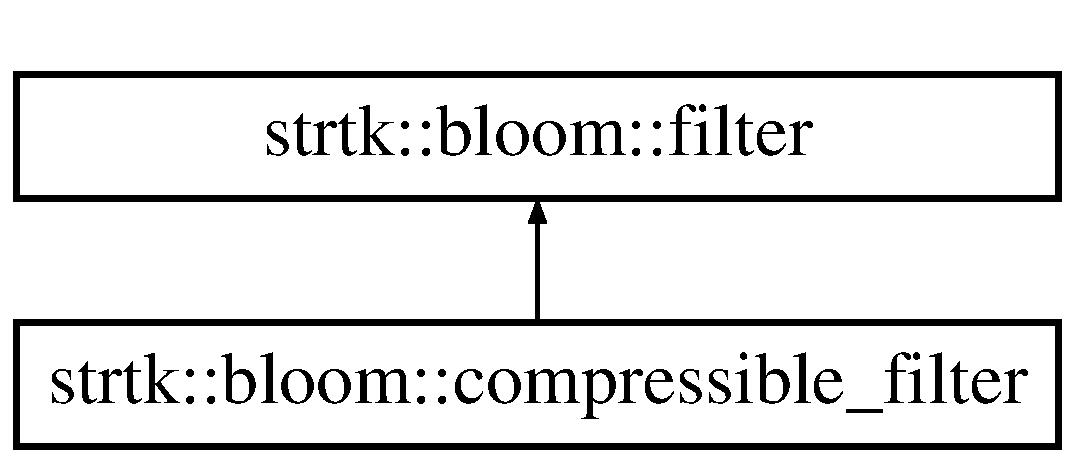
\includegraphics[height=2.000000cm]{classstrtk_1_1bloom_1_1filter}
\end{center}
\end{figure}
\subsection*{Public Member Functions}
\begin{DoxyCompactItemize}
\item 
\hypertarget{classstrtk_1_1bloom_1_1filter_a752bb5ac59bbb72a6caccdcd0aa50af9}{{\bfseries filter} (const \hyperlink{classstrtk_1_1bloom_1_1parameters}{parameters} \&p)}\label{classstrtk_1_1bloom_1_1filter_a752bb5ac59bbb72a6caccdcd0aa50af9}

\item 
\hypertarget{classstrtk_1_1bloom_1_1filter_a2462cb34bc3ee0f5d55f606bf28e1468}{{\bfseries filter} (const \hyperlink{classstrtk_1_1bloom_1_1filter}{filter} \&\hyperlink{classstrtk_1_1bloom_1_1filter}{filter})}\label{classstrtk_1_1bloom_1_1filter_a2462cb34bc3ee0f5d55f606bf28e1468}

\item 
\hypertarget{classstrtk_1_1bloom_1_1filter_aa2d8739ea23739be5cd34b532b969aad}{bool {\bfseries operator==} (const \hyperlink{classstrtk_1_1bloom_1_1filter}{filter} \&f) const }\label{classstrtk_1_1bloom_1_1filter_aa2d8739ea23739be5cd34b532b969aad}

\item 
\hypertarget{classstrtk_1_1bloom_1_1filter_aae7d76b2e8ccf0abb2f10108bd73d3e2}{bool {\bfseries operator!=} (const \hyperlink{classstrtk_1_1bloom_1_1filter}{filter} \&f) const }\label{classstrtk_1_1bloom_1_1filter_aae7d76b2e8ccf0abb2f10108bd73d3e2}

\item 
\hypertarget{classstrtk_1_1bloom_1_1filter_a40aef1a33538d6fc0559f2663b4cb89e}{\hyperlink{classstrtk_1_1bloom_1_1filter}{filter} \& {\bfseries operator=} (const \hyperlink{classstrtk_1_1bloom_1_1filter}{filter} \&f)}\label{classstrtk_1_1bloom_1_1filter_a40aef1a33538d6fc0559f2663b4cb89e}

\item 
\hypertarget{classstrtk_1_1bloom_1_1filter_ae818512d8324a0face92d2ec6bb6e5a9}{bool {\bfseries operator!} () const }\label{classstrtk_1_1bloom_1_1filter_ae818512d8324a0face92d2ec6bb6e5a9}

\item 
\hypertarget{classstrtk_1_1bloom_1_1filter_ae11aea64449fa1e0bbac52b85f19fb7c}{void {\bfseries clear} ()}\label{classstrtk_1_1bloom_1_1filter_ae11aea64449fa1e0bbac52b85f19fb7c}

\item 
\hypertarget{classstrtk_1_1bloom_1_1filter_a9d5c073bfa7a01fb299ff6fc50139f77}{void {\bfseries insert} (const unsigned char $\ast$key\-\_\-begin, const std\-::size\-\_\-t \&length)}\label{classstrtk_1_1bloom_1_1filter_a9d5c073bfa7a01fb299ff6fc50139f77}

\item 
\hypertarget{classstrtk_1_1bloom_1_1filter_a7384814d47e8969f0ee0420737f2d30e}{{\footnotesize template$<$typename T $>$ }\\void {\bfseries insert} (const T \&t)}\label{classstrtk_1_1bloom_1_1filter_a7384814d47e8969f0ee0420737f2d30e}

\item 
\hypertarget{classstrtk_1_1bloom_1_1filter_a0c6789bceec08fe13f18780ae7a95794}{void {\bfseries insert} (const std\-::string \&key)}\label{classstrtk_1_1bloom_1_1filter_a0c6789bceec08fe13f18780ae7a95794}

\item 
\hypertarget{classstrtk_1_1bloom_1_1filter_ae11f9ff2d525f96fbf73a54360ce2dfc}{void {\bfseries insert} (const char $\ast$data, const std\-::size\-\_\-t \&length)}\label{classstrtk_1_1bloom_1_1filter_ae11f9ff2d525f96fbf73a54360ce2dfc}

\item 
\hypertarget{classstrtk_1_1bloom_1_1filter_ab6709ff6d419246b4783ee3d1b83e774}{{\footnotesize template$<$typename Input\-Iterator $>$ }\\void {\bfseries insert} (const Input\-Iterator begin, const Input\-Iterator end)}\label{classstrtk_1_1bloom_1_1filter_ab6709ff6d419246b4783ee3d1b83e774}

\item 
\hypertarget{classstrtk_1_1bloom_1_1filter_a01d6696b427a79989a233ccac7b93c55}{virtual bool {\bfseries contains} (const unsigned char $\ast$key\-\_\-begin, const std\-::size\-\_\-t length) const }\label{classstrtk_1_1bloom_1_1filter_a01d6696b427a79989a233ccac7b93c55}

\item 
\hypertarget{classstrtk_1_1bloom_1_1filter_a8023755487ce5ab8c0f8d034ff5a08f4}{{\footnotesize template$<$typename T $>$ }\\bool {\bfseries contains} (const T \&t) const }\label{classstrtk_1_1bloom_1_1filter_a8023755487ce5ab8c0f8d034ff5a08f4}

\item 
\hypertarget{classstrtk_1_1bloom_1_1filter_acd1dc0548198ceef2645b58cd9eff5e4}{bool {\bfseries contains} (const std\-::string \&key) const }\label{classstrtk_1_1bloom_1_1filter_acd1dc0548198ceef2645b58cd9eff5e4}

\item 
\hypertarget{classstrtk_1_1bloom_1_1filter_a0c5a99678eaa21d30f45caa29aeefba4}{bool {\bfseries contains} (const char $\ast$data, const std\-::size\-\_\-t \&length) const }\label{classstrtk_1_1bloom_1_1filter_a0c5a99678eaa21d30f45caa29aeefba4}

\item 
\hypertarget{classstrtk_1_1bloom_1_1filter_a7071ffdaea6d5a166ac77e9ee3476941}{{\footnotesize template$<$typename Input\-Iterator $>$ }\\Input\-Iterator {\bfseries contains\-\_\-all} (const Input\-Iterator begin, const Input\-Iterator end) const }\label{classstrtk_1_1bloom_1_1filter_a7071ffdaea6d5a166ac77e9ee3476941}

\item 
\hypertarget{classstrtk_1_1bloom_1_1filter_a98bf8ecd23d94448df11371e921ffc1f}{{\footnotesize template$<$typename Input\-Iterator $>$ }\\Input\-Iterator {\bfseries contains\-\_\-none} (const Input\-Iterator begin, const Input\-Iterator end) const }\label{classstrtk_1_1bloom_1_1filter_a98bf8ecd23d94448df11371e921ffc1f}

\item 
\hypertarget{classstrtk_1_1bloom_1_1filter_a4b02261a990c573faf4f1e7e7159e0d7}{virtual unsigned long long int {\bfseries size} () const }\label{classstrtk_1_1bloom_1_1filter_a4b02261a990c573faf4f1e7e7159e0d7}

\item 
\hypertarget{classstrtk_1_1bloom_1_1filter_a6d956a30abb41d0cf2a0194f7d1f448f}{std\-::size\-\_\-t {\bfseries element\-\_\-count} () const }\label{classstrtk_1_1bloom_1_1filter_a6d956a30abb41d0cf2a0194f7d1f448f}

\item 
\hypertarget{classstrtk_1_1bloom_1_1filter_af05331a518553986056be1be03b1b3ed}{double {\bfseries effective\-\_\-fpp} () const }\label{classstrtk_1_1bloom_1_1filter_af05331a518553986056be1be03b1b3ed}

\item 
\hypertarget{classstrtk_1_1bloom_1_1filter_a1cca07541a5dcdd12ea7e25491503b92}{\hyperlink{classstrtk_1_1bloom_1_1filter}{filter} \& {\bfseries operator\&=} (const \hyperlink{classstrtk_1_1bloom_1_1filter}{filter} \&f)}\label{classstrtk_1_1bloom_1_1filter_a1cca07541a5dcdd12ea7e25491503b92}

\item 
\hypertarget{classstrtk_1_1bloom_1_1filter_a2e9540cf1eabeb0dd7a39348c8f34714}{\hyperlink{classstrtk_1_1bloom_1_1filter}{filter} \& {\bfseries operator$\vert$=} (const \hyperlink{classstrtk_1_1bloom_1_1filter}{filter} \&f)}\label{classstrtk_1_1bloom_1_1filter_a2e9540cf1eabeb0dd7a39348c8f34714}

\item 
\hypertarget{classstrtk_1_1bloom_1_1filter_afa2edc38e99e2be9facce335d7acb891}{\hyperlink{classstrtk_1_1bloom_1_1filter}{filter} \& {\bfseries operator$^\wedge$=} (const \hyperlink{classstrtk_1_1bloom_1_1filter}{filter} \&f)}\label{classstrtk_1_1bloom_1_1filter_afa2edc38e99e2be9facce335d7acb891}

\item 
\hypertarget{classstrtk_1_1bloom_1_1filter_a35412b17f0e8f67df4cb45948ed04892}{const cell\-\_\-type $\ast$ {\bfseries table} () const }\label{classstrtk_1_1bloom_1_1filter_a35412b17f0e8f67df4cb45948ed04892}

\item 
\hypertarget{classstrtk_1_1bloom_1_1filter_a464d7a8d335ac4f6c33ea56cabbe5fb9}{bool {\bfseries write\-\_\-to\-\_\-file} (const std\-::string \&file\-\_\-name) const }\label{classstrtk_1_1bloom_1_1filter_a464d7a8d335ac4f6c33ea56cabbe5fb9}

\item 
\hypertarget{classstrtk_1_1bloom_1_1filter_ace6e731b6e8caefb14770087cce2ca52}{bool {\bfseries read\-\_\-from\-\_\-file} (const std\-::string \&file\-\_\-name)}\label{classstrtk_1_1bloom_1_1filter_ace6e731b6e8caefb14770087cce2ca52}

\item 
\hypertarget{classstrtk_1_1bloom_1_1filter_adbbb839e64567879288981e34f37bae4}{std\-::size\-\_\-t {\bfseries hash\-\_\-count} ()}\label{classstrtk_1_1bloom_1_1filter_adbbb839e64567879288981e34f37bae4}

\end{DoxyCompactItemize}
\subsection*{Protected Types}
\begin{DoxyCompactItemize}
\item 
\hypertarget{classstrtk_1_1bloom_1_1filter_a1b78a2987ff5657faf0a729bcb1c8f3a}{typedef unsigned int {\bfseries bloom\-\_\-type}}\label{classstrtk_1_1bloom_1_1filter_a1b78a2987ff5657faf0a729bcb1c8f3a}

\item 
\hypertarget{classstrtk_1_1bloom_1_1filter_aa937c83c9315bd79e25a03b2cca68e4f}{typedef unsigned char {\bfseries cell\-\_\-type}}\label{classstrtk_1_1bloom_1_1filter_aa937c83c9315bd79e25a03b2cca68e4f}

\end{DoxyCompactItemize}
\subsection*{Protected Member Functions}
\begin{DoxyCompactItemize}
\item 
\hypertarget{classstrtk_1_1bloom_1_1filter_a10bdf2999e326607ec004fa855fbcc36}{virtual void {\bfseries compute\-\_\-indices} (const bloom\-\_\-type \&hash, std\-::size\-\_\-t \&bit\-\_\-index, std\-::size\-\_\-t \&bit) const }\label{classstrtk_1_1bloom_1_1filter_a10bdf2999e326607ec004fa855fbcc36}

\item 
\hypertarget{classstrtk_1_1bloom_1_1filter_ae0f781b16fd20e5ce5453cafae1a8ae9}{void {\bfseries generate\-\_\-unique\-\_\-salt} ()}\label{classstrtk_1_1bloom_1_1filter_ae0f781b16fd20e5ce5453cafae1a8ae9}

\item 
\hypertarget{classstrtk_1_1bloom_1_1filter_a22f76cc997cf2eb97741261fff575354}{bloom\-\_\-type {\bfseries hash\-\_\-ap} (const unsigned char $\ast$begin, std\-::size\-\_\-t remaining\-\_\-length, bloom\-\_\-type hash) const }\label{classstrtk_1_1bloom_1_1filter_a22f76cc997cf2eb97741261fff575354}

\end{DoxyCompactItemize}
\subsection*{Protected Attributes}
\begin{DoxyCompactItemize}
\item 
\hypertarget{classstrtk_1_1bloom_1_1filter_a4e56d8cfa2246773de801b76d844dfaa}{std\-::vector$<$ bloom\-\_\-type $>$ {\bfseries salt\-\_\-}}\label{classstrtk_1_1bloom_1_1filter_a4e56d8cfa2246773de801b76d844dfaa}

\item 
\hypertarget{classstrtk_1_1bloom_1_1filter_a7dc90f110481fb3b0f4f322f9ba13ee3}{unsigned char $\ast$ {\bfseries bit\-\_\-table\-\_\-}}\label{classstrtk_1_1bloom_1_1filter_a7dc90f110481fb3b0f4f322f9ba13ee3}

\item 
\hypertarget{classstrtk_1_1bloom_1_1filter_aca6a283ed1ee823590acb0a436d66992}{unsigned int {\bfseries salt\-\_\-count\-\_\-}}\label{classstrtk_1_1bloom_1_1filter_aca6a283ed1ee823590acb0a436d66992}

\item 
\hypertarget{classstrtk_1_1bloom_1_1filter_a246589ad0484a1f404cc0fbaf8af5b77}{unsigned long long int {\bfseries table\-\_\-size\-\_\-}}\label{classstrtk_1_1bloom_1_1filter_a246589ad0484a1f404cc0fbaf8af5b77}

\item 
\hypertarget{classstrtk_1_1bloom_1_1filter_a11aaab2270381c209f33f6b08b270774}{unsigned long long int {\bfseries raw\-\_\-table\-\_\-size\-\_\-}}\label{classstrtk_1_1bloom_1_1filter_a11aaab2270381c209f33f6b08b270774}

\item 
\hypertarget{classstrtk_1_1bloom_1_1filter_afda5f7534a7187b489d083255384088b}{unsigned long long int {\bfseries projected\-\_\-element\-\_\-count\-\_\-}}\label{classstrtk_1_1bloom_1_1filter_afda5f7534a7187b489d083255384088b}

\item 
\hypertarget{classstrtk_1_1bloom_1_1filter_a7b5c4600a831c4df9ebe02f34b112c99}{unsigned int {\bfseries inserted\-\_\-element\-\_\-count\-\_\-}}\label{classstrtk_1_1bloom_1_1filter_a7b5c4600a831c4df9ebe02f34b112c99}

\item 
\hypertarget{classstrtk_1_1bloom_1_1filter_aab43485401a79261931e8577e531bc62}{unsigned long long int {\bfseries random\-\_\-seed\-\_\-}}\label{classstrtk_1_1bloom_1_1filter_aab43485401a79261931e8577e531bc62}

\item 
\hypertarget{classstrtk_1_1bloom_1_1filter_aa6e22e400251d1f29427b1af89fcc82c}{double {\bfseries desired\-\_\-false\-\_\-positive\-\_\-probability\-\_\-}}\label{classstrtk_1_1bloom_1_1filter_aa6e22e400251d1f29427b1af89fcc82c}

\end{DoxyCompactItemize}


The documentation for this class was generated from the following file\-:\begin{DoxyCompactItemize}
\item 
strtk.\-hpp\end{DoxyCompactItemize}

\hypertarget{structstrtk_1_1filter__non__empty__range}{\section{strtk\-:\-:filter\-\_\-non\-\_\-empty\-\_\-range$<$ Output\-Iterator $>$ Struct Template Reference}
\label{structstrtk_1_1filter__non__empty__range}\index{strtk\-::filter\-\_\-non\-\_\-empty\-\_\-range$<$ Output\-Iterator $>$@{strtk\-::filter\-\_\-non\-\_\-empty\-\_\-range$<$ Output\-Iterator $>$}}
}
\subsection*{Public Member Functions}
\begin{DoxyCompactItemize}
\item 
\hypertarget{structstrtk_1_1filter__non__empty__range_af8c6b151212f98ef7445aae995244d2e}{{\bfseries filter\-\_\-non\-\_\-empty\-\_\-range} (Output\-Iterator out)}\label{structstrtk_1_1filter__non__empty__range_af8c6b151212f98ef7445aae995244d2e}

\item 
\hypertarget{structstrtk_1_1filter__non__empty__range_ac7079947ac98e16361a263275c8f3291}{{\footnotesize template$<$typename Iterator $>$ }\\void {\bfseries operator()} (const std\-::pair$<$ Iterator, Iterator $>$ \&range)}\label{structstrtk_1_1filter__non__empty__range_ac7079947ac98e16361a263275c8f3291}

\end{DoxyCompactItemize}


The documentation for this struct was generated from the following file\-:\begin{DoxyCompactItemize}
\item 
strtk.\-hpp\end{DoxyCompactItemize}

\hypertarget{structstrtk_1_1filter__on__match}{\section{strtk\-:\-:filter\-\_\-on\-\_\-match$<$ Output\-Predicate $>$ Struct Template Reference}
\label{structstrtk_1_1filter__on__match}\index{strtk\-::filter\-\_\-on\-\_\-match$<$ Output\-Predicate $>$@{strtk\-::filter\-\_\-on\-\_\-match$<$ Output\-Predicate $>$}}
}
\subsection*{Public Member Functions}
\begin{DoxyCompactItemize}
\item 
\hypertarget{structstrtk_1_1filter__on__match_ac2bc7ea1b5054a5db44ccb3878958475}{{\bfseries filter\-\_\-on\-\_\-match} (const std\-::string $\ast$begin, const std\-::string $\ast$end, Output\-Predicate predicate, bool case\-\_\-insensitive, bool allow\-\_\-through\-\_\-on\-\_\-match=true)}\label{structstrtk_1_1filter__on__match_ac2bc7ea1b5054a5db44ccb3878958475}

\item 
\hypertarget{structstrtk_1_1filter__on__match_aa0175e5f6a4080e4fefc669e3700f972}{{\footnotesize template$<$typename Iterator $>$ }\\void {\bfseries operator()} (const std\-::pair$<$ Iterator, Iterator $>$ \&range) const }\label{structstrtk_1_1filter__on__match_aa0175e5f6a4080e4fefc669e3700f972}

\item 
\hypertarget{structstrtk_1_1filter__on__match_a5a45989738a76604b3edc0fddf95e899}{void {\bfseries operator()} (const std\-::string \&s) const }\label{structstrtk_1_1filter__on__match_a5a45989738a76604b3edc0fddf95e899}

\end{DoxyCompactItemize}


The documentation for this struct was generated from the following file\-:\begin{DoxyCompactItemize}
\item 
strtk.\-hpp\end{DoxyCompactItemize}

\hypertarget{structstrtk_1_1filter__on__wildcard__match}{\section{strtk\-:\-:filter\-\_\-on\-\_\-wildcard\-\_\-match$<$ Output\-Predicate $>$ Struct Template Reference}
\label{structstrtk_1_1filter__on__wildcard__match}\index{strtk\-::filter\-\_\-on\-\_\-wildcard\-\_\-match$<$ Output\-Predicate $>$@{strtk\-::filter\-\_\-on\-\_\-wildcard\-\_\-match$<$ Output\-Predicate $>$}}
}
\subsection*{Public Member Functions}
\begin{DoxyCompactItemize}
\item 
\hypertarget{structstrtk_1_1filter__on__wildcard__match_a8cd187af8317197d2d740c0abe00aaec}{{\bfseries filter\-\_\-on\-\_\-wildcard\-\_\-match} (const std\-::string \&match\-\_\-pattern, Output\-Predicate \&predicate, bool allow\-\_\-through\-\_\-on\-\_\-match=true)}\label{structstrtk_1_1filter__on__wildcard__match_a8cd187af8317197d2d740c0abe00aaec}

\item 
\hypertarget{structstrtk_1_1filter__on__wildcard__match_a8482b3e530f3bf22f2d0406a96a109ab}{{\footnotesize template$<$typename Iterator $>$ }\\void {\bfseries operator()} (const std\-::pair$<$ Iterator, Iterator $>$ \&range) const }\label{structstrtk_1_1filter__on__wildcard__match_a8482b3e530f3bf22f2d0406a96a109ab}

\item 
\hypertarget{structstrtk_1_1filter__on__wildcard__match_aab3b857999492671d37e4a6d76470c5f}{void {\bfseries operator()} (const std\-::string \&s) const }\label{structstrtk_1_1filter__on__wildcard__match_aab3b857999492671d37e4a6d76470c5f}

\end{DoxyCompactItemize}


The documentation for this struct was generated from the following file\-:\begin{DoxyCompactItemize}
\item 
strtk.\-hpp\end{DoxyCompactItemize}

\hypertarget{classstrtk_1_1functional__inserter__iterator}{\section{strtk\-:\-:functional\-\_\-inserter\-\_\-iterator$<$ Function $>$ Class Template Reference}
\label{classstrtk_1_1functional__inserter__iterator}\index{strtk\-::functional\-\_\-inserter\-\_\-iterator$<$ Function $>$@{strtk\-::functional\-\_\-inserter\-\_\-iterator$<$ Function $>$}}
}
Inheritance diagram for strtk\-:\-:functional\-\_\-inserter\-\_\-iterator$<$ Function $>$\-:\begin{figure}[H]
\begin{center}
\leavevmode
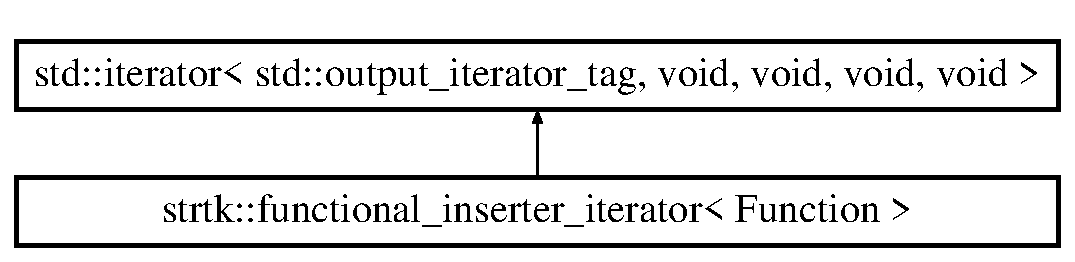
\includegraphics[height=2.000000cm]{classstrtk_1_1functional__inserter__iterator}
\end{center}
\end{figure}
\subsection*{Public Member Functions}
\begin{DoxyCompactItemize}
\item 
\hypertarget{classstrtk_1_1functional__inserter__iterator_a5911baf691923d5b06e8892c96a0ced3}{{\bfseries functional\-\_\-inserter\-\_\-iterator} (Function function)}\label{classstrtk_1_1functional__inserter__iterator_a5911baf691923d5b06e8892c96a0ced3}

\item 
\hypertarget{classstrtk_1_1functional__inserter__iterator_a96341e6c900bd3305da78fe31a7108f9}{{\bfseries functional\-\_\-inserter\-\_\-iterator} (const \hyperlink{classstrtk_1_1functional__inserter__iterator}{functional\-\_\-inserter\-\_\-iterator} \&itr)}\label{classstrtk_1_1functional__inserter__iterator_a96341e6c900bd3305da78fe31a7108f9}

\item 
\hypertarget{classstrtk_1_1functional__inserter__iterator_aedb655893075089c08c82a82a938a046}{\hyperlink{classstrtk_1_1functional__inserter__iterator}{functional\-\_\-inserter\-\_\-iterator} \& {\bfseries operator=} (const \hyperlink{classstrtk_1_1functional__inserter__iterator}{functional\-\_\-inserter\-\_\-iterator} \&itr)}\label{classstrtk_1_1functional__inserter__iterator_aedb655893075089c08c82a82a938a046}

\item 
\hypertarget{classstrtk_1_1functional__inserter__iterator_a20430ca728937df9e4f47fd8516685e9}{{\footnotesize template$<$typename T $>$ }\\\hyperlink{classstrtk_1_1functional__inserter__iterator}{functional\-\_\-inserter\-\_\-iterator} \& {\bfseries operator=} (const T \&t)}\label{classstrtk_1_1functional__inserter__iterator_a20430ca728937df9e4f47fd8516685e9}

\item 
\hypertarget{classstrtk_1_1functional__inserter__iterator_a73881ddd665ed765eb9df9ab228f4de0}{{\footnotesize template$<$typename T $>$ }\\void {\bfseries operator()} (const T \&t)}\label{classstrtk_1_1functional__inserter__iterator_a73881ddd665ed765eb9df9ab228f4de0}

\item 
\hypertarget{classstrtk_1_1functional__inserter__iterator_acb8c6f3aaf05c232cbb9b0224d13cdd9}{\hyperlink{classstrtk_1_1functional__inserter__iterator}{functional\-\_\-inserter\-\_\-iterator} \& {\bfseries operator$\ast$} ()}\label{classstrtk_1_1functional__inserter__iterator_acb8c6f3aaf05c232cbb9b0224d13cdd9}

\item 
\hypertarget{classstrtk_1_1functional__inserter__iterator_a6da88e0fe992652fb1d47394d645aa71}{\hyperlink{classstrtk_1_1functional__inserter__iterator}{functional\-\_\-inserter\-\_\-iterator} \& {\bfseries operator++} ()}\label{classstrtk_1_1functional__inserter__iterator_a6da88e0fe992652fb1d47394d645aa71}

\item 
\hypertarget{classstrtk_1_1functional__inserter__iterator_a25bda9f590b6d5023d366eabf8adda7a}{\hyperlink{classstrtk_1_1functional__inserter__iterator}{functional\-\_\-inserter\-\_\-iterator} {\bfseries operator++} (int)}\label{classstrtk_1_1functional__inserter__iterator_a25bda9f590b6d5023d366eabf8adda7a}

\end{DoxyCompactItemize}


The documentation for this class was generated from the following file\-:\begin{DoxyCompactItemize}
\item 
strtk.\-hpp\end{DoxyCompactItemize}

\hypertarget{structstrtk_1_1details_1_1hex__number__type__tag}{\section{strtk\-:\-:details\-:\-:hex\-\_\-number\-\_\-type\-\_\-tag Struct Reference}
\label{structstrtk_1_1details_1_1hex__number__type__tag}\index{strtk\-::details\-::hex\-\_\-number\-\_\-type\-\_\-tag@{strtk\-::details\-::hex\-\_\-number\-\_\-type\-\_\-tag}}
}


The documentation for this struct was generated from the following file\-:\begin{DoxyCompactItemize}
\item 
strtk.\-hpp\end{DoxyCompactItemize}

\hypertarget{structstrtk_1_1details_1_1hex__string__type__tag}{\section{strtk\-:\-:details\-:\-:hex\-\_\-string\-\_\-type\-\_\-tag Struct Reference}
\label{structstrtk_1_1details_1_1hex__string__type__tag}\index{strtk\-::details\-::hex\-\_\-string\-\_\-type\-\_\-tag@{strtk\-::details\-::hex\-\_\-string\-\_\-type\-\_\-tag}}
}


The documentation for this struct was generated from the following file\-:\begin{DoxyCompactItemize}
\item 
strtk.\-hpp\end{DoxyCompactItemize}

\hypertarget{classstrtk_1_1hex__to__number__sink}{\section{strtk\-:\-:hex\-\_\-to\-\_\-number\-\_\-sink$<$ T $>$ Class Template Reference}
\label{classstrtk_1_1hex__to__number__sink}\index{strtk\-::hex\-\_\-to\-\_\-number\-\_\-sink$<$ T $>$@{strtk\-::hex\-\_\-to\-\_\-number\-\_\-sink$<$ T $>$}}
}
\subsection*{Public Member Functions}
\begin{DoxyCompactItemize}
\item 
\hypertarget{classstrtk_1_1hex__to__number__sink_ae7f365203f38fbd5ccd43e5e6ba28685}{{\bfseries hex\-\_\-to\-\_\-number\-\_\-sink} (T \&t)}\label{classstrtk_1_1hex__to__number__sink_ae7f365203f38fbd5ccd43e5e6ba28685}

\item 
\hypertarget{classstrtk_1_1hex__to__number__sink_ace194656c2d8303ecb27c9116148b9c4}{{\bfseries hex\-\_\-to\-\_\-number\-\_\-sink} (const \hyperlink{classstrtk_1_1hex__to__number__sink}{hex\-\_\-to\-\_\-number\-\_\-sink} \&hns)}\label{classstrtk_1_1hex__to__number__sink_ace194656c2d8303ecb27c9116148b9c4}

\item 
\hypertarget{classstrtk_1_1hex__to__number__sink_a8b088b6f9b0a3ae942661ecf727db5b5}{\hyperlink{classstrtk_1_1hex__to__number__sink}{hex\-\_\-to\-\_\-number\-\_\-sink} \& {\bfseries operator=} (const \hyperlink{classstrtk_1_1hex__to__number__sink}{hex\-\_\-to\-\_\-number\-\_\-sink} \&hns)}\label{classstrtk_1_1hex__to__number__sink_a8b088b6f9b0a3ae942661ecf727db5b5}

\item 
\hypertarget{classstrtk_1_1hex__to__number__sink_a819bcf5f2aa99f5f3810bccbe6449583}{{\footnotesize template$<$typename Input\-Iterator $>$ }\\\hyperlink{classstrtk_1_1hex__to__number__sink}{hex\-\_\-to\-\_\-number\-\_\-sink} \& {\bfseries operator=} (const std\-::pair$<$ Input\-Iterator, Input\-Iterator $>$ \&s)}\label{classstrtk_1_1hex__to__number__sink_a819bcf5f2aa99f5f3810bccbe6449583}

\item 
\hypertarget{classstrtk_1_1hex__to__number__sink_a81593e6bf0e47811dbbd4f0c78726054}{\hyperlink{classstrtk_1_1hex__to__number__sink}{hex\-\_\-to\-\_\-number\-\_\-sink} \& {\bfseries operator=} (const std\-::string \&s)}\label{classstrtk_1_1hex__to__number__sink_a81593e6bf0e47811dbbd4f0c78726054}

\item 
\hypertarget{classstrtk_1_1hex__to__number__sink_abb107c0a5139f6457fa2286da2297078}{bool {\bfseries valid} () const }\label{classstrtk_1_1hex__to__number__sink_abb107c0a5139f6457fa2286da2297078}

\end{DoxyCompactItemize}


The documentation for this class was generated from the following file\-:\begin{DoxyCompactItemize}
\item 
strtk.\-hpp\end{DoxyCompactItemize}

\hypertarget{classstrtk_1_1hex__to__string__sink}{\section{strtk\-:\-:hex\-\_\-to\-\_\-string\-\_\-sink Class Reference}
\label{classstrtk_1_1hex__to__string__sink}\index{strtk\-::hex\-\_\-to\-\_\-string\-\_\-sink@{strtk\-::hex\-\_\-to\-\_\-string\-\_\-sink}}
}
\subsection*{Public Member Functions}
\begin{DoxyCompactItemize}
\item 
\hypertarget{classstrtk_1_1hex__to__string__sink_ac48595e8b2f269fd3b9aa647019172c1}{{\bfseries hex\-\_\-to\-\_\-string\-\_\-sink} (std\-::string \&s)}\label{classstrtk_1_1hex__to__string__sink_ac48595e8b2f269fd3b9aa647019172c1}

\item 
\hypertarget{classstrtk_1_1hex__to__string__sink_a4be66604644b0f1540a6471419df161c}{{\bfseries hex\-\_\-to\-\_\-string\-\_\-sink} (const \hyperlink{classstrtk_1_1hex__to__string__sink}{hex\-\_\-to\-\_\-string\-\_\-sink} \&hss)}\label{classstrtk_1_1hex__to__string__sink_a4be66604644b0f1540a6471419df161c}

\item 
\hypertarget{classstrtk_1_1hex__to__string__sink_ab7b070dea47e95cd81674ce7591feb3d}{\hyperlink{classstrtk_1_1hex__to__string__sink}{hex\-\_\-to\-\_\-string\-\_\-sink} \& {\bfseries operator=} (const \hyperlink{classstrtk_1_1hex__to__string__sink}{hex\-\_\-to\-\_\-string\-\_\-sink} \&hss)}\label{classstrtk_1_1hex__to__string__sink_ab7b070dea47e95cd81674ce7591feb3d}

\item 
\hypertarget{classstrtk_1_1hex__to__string__sink_a8878d9c585d58853e692eda72db2a440}{{\footnotesize template$<$typename Input\-Iterator $>$ }\\\hyperlink{classstrtk_1_1hex__to__string__sink}{hex\-\_\-to\-\_\-string\-\_\-sink} \& {\bfseries operator=} (const std\-::pair$<$ Input\-Iterator, Input\-Iterator $>$ \&s)}\label{classstrtk_1_1hex__to__string__sink_a8878d9c585d58853e692eda72db2a440}

\item 
\hypertarget{classstrtk_1_1hex__to__string__sink_a8d437ad10292cd021ec20320eb726eb9}{\hyperlink{classstrtk_1_1hex__to__string__sink}{hex\-\_\-to\-\_\-string\-\_\-sink} \& {\bfseries operator=} (const std\-::string \&s)}\label{classstrtk_1_1hex__to__string__sink_a8d437ad10292cd021ec20320eb726eb9}

\item 
\hypertarget{classstrtk_1_1hex__to__string__sink_af97651791a55643dd907c514b5056ccb}{bool {\bfseries valid} () const }\label{classstrtk_1_1hex__to__string__sink_af97651791a55643dd907c514b5056ccb}

\end{DoxyCompactItemize}


The documentation for this class was generated from the following file\-:\begin{DoxyCompactItemize}
\item 
strtk.\-hpp\end{DoxyCompactItemize}

\hypertarget{classstrtk_1_1details_1_1iexpect__impl}{\section{strtk\-:\-:details\-:\-:iexpect\-\_\-impl Class Reference}
\label{classstrtk_1_1details_1_1iexpect__impl}\index{strtk\-::details\-::iexpect\-\_\-impl@{strtk\-::details\-::iexpect\-\_\-impl}}
}
\subsection*{Public Member Functions}
\begin{DoxyCompactItemize}
\item 
\hypertarget{classstrtk_1_1details_1_1iexpect__impl_a916f2895766f89ba8cdaa1b41d92855e}{{\bfseries iexpect\-\_\-impl} (const std\-::string \&s)}\label{classstrtk_1_1details_1_1iexpect__impl_a916f2895766f89ba8cdaa1b41d92855e}

\item 
\hypertarget{classstrtk_1_1details_1_1iexpect__impl_ae8cac250ad5fcd5ba7e12da5b6ca391b}{{\footnotesize template$<$typename Input\-Iterator $>$ }\\bool {\bfseries operator()} (Input\-Iterator begin, Input\-Iterator end)}\label{classstrtk_1_1details_1_1iexpect__impl_ae8cac250ad5fcd5ba7e12da5b6ca391b}

\item 
\hypertarget{classstrtk_1_1details_1_1iexpect__impl_a5ddd926e05ab0baf38c21964eb100cab}{\hyperlink{classstrtk_1_1details_1_1iexpect__impl}{iexpect\-\_\-impl} \& {\bfseries ref} ()}\label{classstrtk_1_1details_1_1iexpect__impl_a5ddd926e05ab0baf38c21964eb100cab}

\item 
\hypertarget{classstrtk_1_1details_1_1iexpect__impl_a85d4550de4f4e64365f5ba24d238bb20}{void {\bfseries set\-\_\-value} (const std\-::string \&s)}\label{classstrtk_1_1details_1_1iexpect__impl_a85d4550de4f4e64365f5ba24d238bb20}

\end{DoxyCompactItemize}


The documentation for this class was generated from the following file\-:\begin{DoxyCompactItemize}
\item 
strtk.\-hpp\end{DoxyCompactItemize}

\hypertarget{classstrtk_1_1ignore__token}{\section{strtk\-:\-:ignore\-\_\-token Class Reference}
\label{classstrtk_1_1ignore__token}\index{strtk\-::ignore\-\_\-token@{strtk\-::ignore\-\_\-token}}
}
\subsection*{Public Member Functions}
\begin{DoxyCompactItemize}
\item 
\hypertarget{classstrtk_1_1ignore__token_a773ce9971728a09ed6371ac11daadb7f}{{\footnotesize template$<$typename Input\-Iterator $>$ }\\\hyperlink{classstrtk_1_1ignore__token}{ignore\-\_\-token} \& {\bfseries operator=} (const std\-::pair$<$ Input\-Iterator, Input\-Iterator $>$ \&)}\label{classstrtk_1_1ignore__token_a773ce9971728a09ed6371ac11daadb7f}

\item 
\hypertarget{classstrtk_1_1ignore__token_aeeaef45e33a650b6c46a69f3e98338b1}{\hyperlink{classstrtk_1_1ignore__token}{ignore\-\_\-token} \& {\bfseries operator=} (const std\-::string \&)}\label{classstrtk_1_1ignore__token_aeeaef45e33a650b6c46a69f3e98338b1}

\end{DoxyCompactItemize}


The documentation for this class was generated from the following file\-:\begin{DoxyCompactItemize}
\item 
strtk.\-hpp\end{DoxyCompactItemize}

\hypertarget{structstrtk_1_1details_1_1ignore__token__type__tag}{\section{strtk\-:\-:details\-:\-:ignore\-\_\-token\-\_\-type\-\_\-tag Struct Reference}
\label{structstrtk_1_1details_1_1ignore__token__type__tag}\index{strtk\-::details\-::ignore\-\_\-token\-\_\-type\-\_\-tag@{strtk\-::details\-::ignore\-\_\-token\-\_\-type\-\_\-tag}}
}


The documentation for this struct was generated from the following file\-:\begin{DoxyCompactItemize}
\item 
strtk.\-hpp\end{DoxyCompactItemize}

\hypertarget{structstrtk_1_1details_1_1index__remover__impl}{\section{strtk\-:\-:details\-:\-:index\-\_\-remover\-\_\-impl$<$ Allocator, Sequence $>$ Struct Template Reference}
\label{structstrtk_1_1details_1_1index__remover__impl}\index{strtk\-::details\-::index\-\_\-remover\-\_\-impl$<$ Allocator, Sequence $>$@{strtk\-::details\-::index\-\_\-remover\-\_\-impl$<$ Allocator, Sequence $>$}}
}
\subsection*{Public Types}
\begin{DoxyCompactItemize}
\item 
\hypertarget{structstrtk_1_1details_1_1index__remover__impl_a952e099a3c83973d0b833388c38393b4}{typedef Sequence$<$ std\-::size\-\_\-t, \\*
Allocator $>$ {\bfseries sequence\-\_\-t}}\label{structstrtk_1_1details_1_1index__remover__impl_a952e099a3c83973d0b833388c38393b4}

\end{DoxyCompactItemize}
\subsection*{Public Member Functions}
\begin{DoxyCompactItemize}
\item 
\hypertarget{structstrtk_1_1details_1_1index__remover__impl_ae2b9113e05294c44c46368b22dbab16d}{{\bfseries index\-\_\-remover\-\_\-impl} (const sequence\-\_\-t \&sequence)}\label{structstrtk_1_1details_1_1index__remover__impl_ae2b9113e05294c44c46368b22dbab16d}

\item 
\hypertarget{structstrtk_1_1details_1_1index__remover__impl_a1554308b4850444ffcf70c74ba5ad626}{{\footnotesize template$<$typename T $>$ }\\bool {\bfseries operator()} (const T \&)}\label{structstrtk_1_1details_1_1index__remover__impl_a1554308b4850444ffcf70c74ba5ad626}

\end{DoxyCompactItemize}
\subsection*{Public Attributes}
\begin{DoxyCompactItemize}
\item 
\hypertarget{structstrtk_1_1details_1_1index__remover__impl_af503307f08fab2eec411485f5646e367}{sequence\-\_\-t\-::const\-\_\-iterator {\bfseries itr\-\_\-}}\label{structstrtk_1_1details_1_1index__remover__impl_af503307f08fab2eec411485f5646e367}

\item 
\hypertarget{structstrtk_1_1details_1_1index__remover__impl_ae20154a16b4b52e682c24a19e257c8b6}{sequence\-\_\-t\-::const\-\_\-iterator {\bfseries end\-\_\-}}\label{structstrtk_1_1details_1_1index__remover__impl_ae20154a16b4b52e682c24a19e257c8b6}

\item 
\hypertarget{structstrtk_1_1details_1_1index__remover__impl_a87d808afad703486a92984a0c4f3078d}{std\-::size\-\_\-t {\bfseries current\-\_\-index\-\_\-}}\label{structstrtk_1_1details_1_1index__remover__impl_a87d808afad703486a92984a0c4f3078d}

\item 
\hypertarget{structstrtk_1_1details_1_1index__remover__impl_a210debd9dd385be69f6630b3167ee6f2}{bool {\bfseries check\-\_\-}}\label{structstrtk_1_1details_1_1index__remover__impl_a210debd9dd385be69f6630b3167ee6f2}

\end{DoxyCompactItemize}


The documentation for this struct was generated from the following file\-:\begin{DoxyCompactItemize}
\item 
strtk.\-hpp\end{DoxyCompactItemize}

\hypertarget{classstrtk_1_1details_1_1inrange__impl}{\section{strtk\-:\-:details\-:\-:inrange\-\_\-impl$<$ T $>$ Class Template Reference}
\label{classstrtk_1_1details_1_1inrange__impl}\index{strtk\-::details\-::inrange\-\_\-impl$<$ T $>$@{strtk\-::details\-::inrange\-\_\-impl$<$ T $>$}}
}
\subsection*{Public Member Functions}
\begin{DoxyCompactItemize}
\item 
\hypertarget{classstrtk_1_1details_1_1inrange__impl_a8fe6d156bcdb972f4c797c8128ee990c}{{\bfseries inrange\-\_\-impl} (T \&t, const T \&low, const T \&hi)}\label{classstrtk_1_1details_1_1inrange__impl_a8fe6d156bcdb972f4c797c8128ee990c}

\item 
\hypertarget{classstrtk_1_1details_1_1inrange__impl_a8babe6b3489c12e8d665cde5aa781e87}{{\footnotesize template$<$typename Input\-Iterator $>$ }\\bool {\bfseries operator()} (Input\-Iterator begin, Input\-Iterator end)}\label{classstrtk_1_1details_1_1inrange__impl_a8babe6b3489c12e8d665cde5aa781e87}

\item 
\hypertarget{classstrtk_1_1details_1_1inrange__impl_a2a9f26c304a5b1f5547b70270cf350c1}{\hyperlink{classstrtk_1_1details_1_1inrange__impl}{inrange\-\_\-impl}$<$ T $>$ \& {\bfseries ref} ()}\label{classstrtk_1_1details_1_1inrange__impl_a2a9f26c304a5b1f5547b70270cf350c1}

\item 
\hypertarget{classstrtk_1_1details_1_1inrange__impl_a3bff748a298b38ad9dd4cd00de6e9149}{void {\bfseries set\-\_\-low\-\_\-hi} (const T \&low, const T \&hi)}\label{classstrtk_1_1details_1_1inrange__impl_a3bff748a298b38ad9dd4cd00de6e9149}

\end{DoxyCompactItemize}


The documentation for this class was generated from the following file\-:\begin{DoxyCompactItemize}
\item 
strtk.\-hpp\end{DoxyCompactItemize}

\hypertarget{structstrtk_1_1details_1_1inrange__type__tag}{\section{strtk\-:\-:details\-:\-:inrange\-\_\-type\-\_\-tag Struct Reference}
\label{structstrtk_1_1details_1_1inrange__type__tag}\index{strtk\-::details\-::inrange\-\_\-type\-\_\-tag@{strtk\-::details\-::inrange\-\_\-type\-\_\-tag}}
}


The documentation for this struct was generated from the following file\-:\begin{DoxyCompactItemize}
\item 
strtk.\-hpp\end{DoxyCompactItemize}

\hypertarget{classstrtk_1_1inserter__with__valuetype__iterator}{\section{strtk\-:\-:inserter\-\_\-with\-\_\-valuetype\-\_\-iterator$<$ Set $>$ Class Template Reference}
\label{classstrtk_1_1inserter__with__valuetype__iterator}\index{strtk\-::inserter\-\_\-with\-\_\-valuetype\-\_\-iterator$<$ Set $>$@{strtk\-::inserter\-\_\-with\-\_\-valuetype\-\_\-iterator$<$ Set $>$}}
}
Inheritance diagram for strtk\-:\-:inserter\-\_\-with\-\_\-valuetype\-\_\-iterator$<$ Set $>$\-:\begin{figure}[H]
\begin{center}
\leavevmode
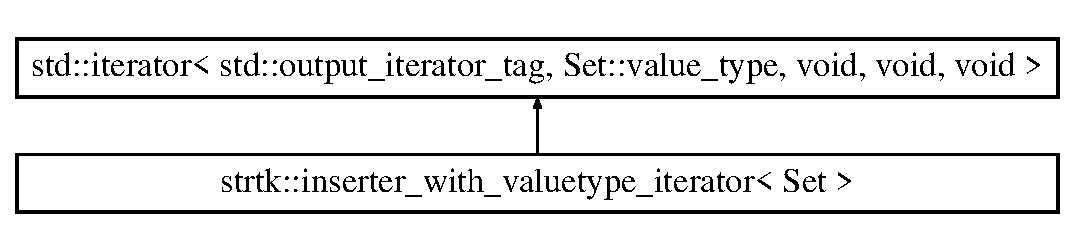
\includegraphics[height=2.000000cm]{classstrtk_1_1inserter__with__valuetype__iterator}
\end{center}
\end{figure}
\subsection*{Public Member Functions}
\begin{DoxyCompactItemize}
\item 
\hypertarget{classstrtk_1_1inserter__with__valuetype__iterator_aecab8b0ca75d5cfc23d42245e2d25357}{{\bfseries inserter\-\_\-with\-\_\-valuetype\-\_\-iterator} (Set \&set)}\label{classstrtk_1_1inserter__with__valuetype__iterator_aecab8b0ca75d5cfc23d42245e2d25357}

\item 
\hypertarget{classstrtk_1_1inserter__with__valuetype__iterator_aa90d59fbbbe0e1bd3e4397a26d986502}{{\bfseries inserter\-\_\-with\-\_\-valuetype\-\_\-iterator} (const \hyperlink{classstrtk_1_1inserter__with__valuetype__iterator}{inserter\-\_\-with\-\_\-valuetype\-\_\-iterator} \&itr)}\label{classstrtk_1_1inserter__with__valuetype__iterator_aa90d59fbbbe0e1bd3e4397a26d986502}

\item 
\hypertarget{classstrtk_1_1inserter__with__valuetype__iterator_a998a63578bf293fb1fc95d82128a5cef}{\hyperlink{classstrtk_1_1inserter__with__valuetype__iterator}{inserter\-\_\-with\-\_\-valuetype\-\_\-iterator} \& {\bfseries operator=} (const \hyperlink{classstrtk_1_1inserter__with__valuetype__iterator}{inserter\-\_\-with\-\_\-valuetype\-\_\-iterator} \&itr)}\label{classstrtk_1_1inserter__with__valuetype__iterator_a998a63578bf293fb1fc95d82128a5cef}

\item 
\hypertarget{classstrtk_1_1inserter__with__valuetype__iterator_a586666811db9b51377a4764c901524f9}{\hyperlink{classstrtk_1_1inserter__with__valuetype__iterator}{inserter\-\_\-with\-\_\-valuetype\-\_\-iterator} \& {\bfseries operator=} (const typename Set\-::value\-\_\-type \&v)}\label{classstrtk_1_1inserter__with__valuetype__iterator_a586666811db9b51377a4764c901524f9}

\item 
\hypertarget{classstrtk_1_1inserter__with__valuetype__iterator_a7ab7ff64e5376644b77ba073bb1de4bc}{void {\bfseries operator()} (const typename Set\-::value\-\_\-type \&v)}\label{classstrtk_1_1inserter__with__valuetype__iterator_a7ab7ff64e5376644b77ba073bb1de4bc}

\item 
\hypertarget{classstrtk_1_1inserter__with__valuetype__iterator_a894b23749335da50a97349ee002bd6e7}{\hyperlink{classstrtk_1_1inserter__with__valuetype__iterator}{inserter\-\_\-with\-\_\-valuetype\-\_\-iterator} \& {\bfseries operator$\ast$} ()}\label{classstrtk_1_1inserter__with__valuetype__iterator_a894b23749335da50a97349ee002bd6e7}

\item 
\hypertarget{classstrtk_1_1inserter__with__valuetype__iterator_a0e272628c58868c156a68906ec4358aa}{\hyperlink{classstrtk_1_1inserter__with__valuetype__iterator}{inserter\-\_\-with\-\_\-valuetype\-\_\-iterator} \& {\bfseries operator++} ()}\label{classstrtk_1_1inserter__with__valuetype__iterator_a0e272628c58868c156a68906ec4358aa}

\item 
\hypertarget{classstrtk_1_1inserter__with__valuetype__iterator_ac975c4e31a74f8c69ae731df097fe3ef}{\hyperlink{classstrtk_1_1inserter__with__valuetype__iterator}{inserter\-\_\-with\-\_\-valuetype\-\_\-iterator} {\bfseries operator++} (int)}\label{classstrtk_1_1inserter__with__valuetype__iterator_ac975c4e31a74f8c69ae731df097fe3ef}

\end{DoxyCompactItemize}


The documentation for this class was generated from the following file\-:\begin{DoxyCompactItemize}
\item 
strtk.\-hpp\end{DoxyCompactItemize}

\hypertarget{structstrtk_1_1interleave__ary}{\section{strtk\-:\-:interleave\-\_\-ary$<$ n $>$ Struct Template Reference}
\label{structstrtk_1_1interleave__ary}\index{strtk\-::interleave\-\_\-ary$<$ n $>$@{strtk\-::interleave\-\_\-ary$<$ n $>$}}
}


The documentation for this struct was generated from the following file\-:\begin{DoxyCompactItemize}
\item 
strtk.\-hpp\end{DoxyCompactItemize}

\hypertarget{structstrtk_1_1interleave__ary_3_01sizeof_07unsigned_01int_08_4}{\section{strtk\-:\-:interleave\-\_\-ary$<$ sizeof(unsigned int)$>$ Struct Template Reference}
\label{structstrtk_1_1interleave__ary_3_01sizeof_07unsigned_01int_08_4}\index{strtk\-::interleave\-\_\-ary$<$ sizeof(unsigned int)$>$@{strtk\-::interleave\-\_\-ary$<$ sizeof(unsigned int)$>$}}
}
\subsection*{Public Types}
\begin{DoxyCompactItemize}
\item 
\hypertarget{structstrtk_1_1interleave__ary_3_01sizeof_07unsigned_01int_08_4_a8767fff05ad99bc68af9a152c15fe035}{typedef unsigned int {\bfseries type}}\label{structstrtk_1_1interleave__ary_3_01sizeof_07unsigned_01int_08_4_a8767fff05ad99bc68af9a152c15fe035}

\end{DoxyCompactItemize}


The documentation for this struct was generated from the following file\-:\begin{DoxyCompactItemize}
\item 
strtk.\-hpp\end{DoxyCompactItemize}

\hypertarget{structstrtk_1_1interleave__ary_3_01sizeof_07unsigned_01long_01long_01int_08_4}{\section{strtk\-:\-:interleave\-\_\-ary$<$ sizeof(unsigned long long int)$>$ Struct Template Reference}
\label{structstrtk_1_1interleave__ary_3_01sizeof_07unsigned_01long_01long_01int_08_4}\index{strtk\-::interleave\-\_\-ary$<$ sizeof(unsigned long long int)$>$@{strtk\-::interleave\-\_\-ary$<$ sizeof(unsigned long long int)$>$}}
}
\subsection*{Public Types}
\begin{DoxyCompactItemize}
\item 
\hypertarget{structstrtk_1_1interleave__ary_3_01sizeof_07unsigned_01long_01long_01int_08_4_a16a70190b15362eac20a30b45cf86269}{typedef unsigned long long int {\bfseries type}}\label{structstrtk_1_1interleave__ary_3_01sizeof_07unsigned_01long_01long_01int_08_4_a16a70190b15362eac20a30b45cf86269}

\end{DoxyCompactItemize}


The documentation for this struct was generated from the following file\-:\begin{DoxyCompactItemize}
\item 
strtk.\-hpp\end{DoxyCompactItemize}

\hypertarget{structstrtk_1_1interleave__ary_3_01sizeof_07unsigned_01short_08_4}{\section{strtk\-:\-:interleave\-\_\-ary$<$ sizeof(unsigned short)$>$ Struct Template Reference}
\label{structstrtk_1_1interleave__ary_3_01sizeof_07unsigned_01short_08_4}\index{strtk\-::interleave\-\_\-ary$<$ sizeof(unsigned short)$>$@{strtk\-::interleave\-\_\-ary$<$ sizeof(unsigned short)$>$}}
}
\subsection*{Public Types}
\begin{DoxyCompactItemize}
\item 
\hypertarget{structstrtk_1_1interleave__ary_3_01sizeof_07unsigned_01short_08_4_ac72c939b8d6c772004bac71b54a0208f}{typedef unsigned short {\bfseries type}}\label{structstrtk_1_1interleave__ary_3_01sizeof_07unsigned_01short_08_4_ac72c939b8d6c772004bac71b54a0208f}

\end{DoxyCompactItemize}


The documentation for this struct was generated from the following file\-:\begin{DoxyCompactItemize}
\item 
strtk.\-hpp\end{DoxyCompactItemize}

\hypertarget{structstrtk_1_1interval__inserter}{\section{strtk\-:\-:interval\-\_\-inserter$<$ T $>$ Struct Template Reference}
\label{structstrtk_1_1interval__inserter}\index{strtk\-::interval\-\_\-inserter$<$ T $>$@{strtk\-::interval\-\_\-inserter$<$ T $>$}}
}
\subsection*{Public Types}
\begin{DoxyCompactItemize}
\item 
\hypertarget{structstrtk_1_1interval__inserter_a1dba0130eae6769dc258e4b07333c6a9}{typedef T {\bfseries type}}\label{structstrtk_1_1interval__inserter_a1dba0130eae6769dc258e4b07333c6a9}

\end{DoxyCompactItemize}
\subsection*{Public Member Functions}
\begin{DoxyCompactItemize}
\item 
\hypertarget{structstrtk_1_1interval__inserter_a98237e47c9530b9c41755319c85950ff}{{\bfseries interval\-\_\-inserter} (const std\-::size\-\_\-t \&interval, const T \&t)}\label{structstrtk_1_1interval__inserter_a98237e47c9530b9c41755319c85950ff}

\item 
\hypertarget{structstrtk_1_1interval__inserter_af05a2e0a2698da29faa0c6a1aba6e238}{bool {\bfseries operator()} (const type \&)}\label{structstrtk_1_1interval__inserter_af05a2e0a2698da29faa0c6a1aba6e238}

\item 
\hypertarget{structstrtk_1_1interval__inserter_a82a5e17831953a6aad3cf0924e73c8b3}{T {\bfseries operator()} ()}\label{structstrtk_1_1interval__inserter_a82a5e17831953a6aad3cf0924e73c8b3}

\end{DoxyCompactItemize}


The documentation for this struct was generated from the following file\-:\begin{DoxyCompactItemize}
\item 
strtk.\-hpp\end{DoxyCompactItemize}

\hypertarget{structstrtk_1_1details_1_1is__pod}{\section{strtk\-:\-:details\-:\-:is\-\_\-pod$<$ T $>$ Struct Template Reference}
\label{structstrtk_1_1details_1_1is__pod}\index{strtk\-::details\-::is\-\_\-pod$<$ T $>$@{strtk\-::details\-::is\-\_\-pod$<$ T $>$}}
}
\subsection*{Public Types}
\begin{DoxyCompactItemize}
\item 
enum \{ {\bfseries result} = false
 \}
\item 
\hypertarget{structstrtk_1_1details_1_1is__pod_ac680d169b20bf14bfb8efb1cd4c76337}{typedef \hyperlink{structstrtk_1_1details_1_1no__t}{no\-\_\-t} {\bfseries result\-\_\-t}}\label{structstrtk_1_1details_1_1is__pod_ac680d169b20bf14bfb8efb1cd4c76337}

\end{DoxyCompactItemize}


The documentation for this struct was generated from the following file\-:\begin{DoxyCompactItemize}
\item 
strtk.\-hpp\end{DoxyCompactItemize}

\hypertarget{structstrtk_1_1details_1_1is__stl__container}{\section{strtk\-:\-:details\-:\-:is\-\_\-stl\-\_\-container$<$ T $>$ Struct Template Reference}
\label{structstrtk_1_1details_1_1is__stl__container}\index{strtk\-::details\-::is\-\_\-stl\-\_\-container$<$ T $>$@{strtk\-::details\-::is\-\_\-stl\-\_\-container$<$ T $>$}}
}
\subsection*{Public Types}
\begin{DoxyCompactItemize}
\item 
\hypertarget{structstrtk_1_1details_1_1is__stl__container_aa5f8f1ce1b84aad7156aed004b057c94}{typedef \hyperlink{structstrtk_1_1details_1_1no__t}{no\-\_\-t} {\bfseries result\-\_\-t}}\label{structstrtk_1_1details_1_1is__stl__container_aa5f8f1ce1b84aad7156aed004b057c94}

\end{DoxyCompactItemize}


The documentation for this struct was generated from the following file\-:\begin{DoxyCompactItemize}
\item 
strtk.\-hpp\end{DoxyCompactItemize}

\hypertarget{structstrtk_1_1details_1_1is__valid__iterator}{\section{strtk\-:\-:details\-:\-:is\-\_\-valid\-\_\-iterator$<$ T $>$ Struct Template Reference}
\label{structstrtk_1_1details_1_1is__valid__iterator}\index{strtk\-::details\-::is\-\_\-valid\-\_\-iterator$<$ T $>$@{strtk\-::details\-::is\-\_\-valid\-\_\-iterator$<$ T $>$}}
}
\subsection*{Public Types}
\begin{DoxyCompactItemize}
\item 
\hypertarget{structstrtk_1_1details_1_1is__valid__iterator_ac308c7879815462dfe52434ab338d4df}{typedef \hyperlink{structstrtk_1_1details_1_1enable__if}{details\-::enable\-\_\-if}\\*
$<$ \hyperlink{structstrtk_1_1details_1_1supported__iterator__type}{details\-::supported\-\_\-iterator\-\_\-type}\\*
$<$ T $>$\-::value, T $>$\-::type {\bfseries type}}\label{structstrtk_1_1details_1_1is__valid__iterator_ac308c7879815462dfe52434ab338d4df}

\end{DoxyCompactItemize}


The documentation for this struct was generated from the following file\-:\begin{DoxyCompactItemize}
\item 
strtk.\-hpp\end{DoxyCompactItemize}

\hypertarget{classstrtk_1_1keyvalue_1_1key__map}{\section{strtk\-:\-:keyvalue\-:\-:key\-\_\-map$<$ Key\-Type, Map\-Type, Key\-Validator, Value\-Validator $>$ Class Template Reference}
\label{classstrtk_1_1keyvalue_1_1key__map}\index{strtk\-::keyvalue\-::key\-\_\-map$<$ Key\-Type, Map\-Type, Key\-Validator, Value\-Validator $>$@{strtk\-::keyvalue\-::key\-\_\-map$<$ Key\-Type, Map\-Type, Key\-Validator, Value\-Validator $>$}}
}
\subsection*{Public Types}
\begin{DoxyCompactItemize}
\item 
\hypertarget{classstrtk_1_1keyvalue_1_1key__map_a3a53e286dc7cb9d6b43d3d969636b0fa}{typedef Key\-Type {\bfseries key\-\_\-type}}\label{classstrtk_1_1keyvalue_1_1key__map_a3a53e286dc7cb9d6b43d3d969636b0fa}

\item 
\hypertarget{classstrtk_1_1keyvalue_1_1key__map_a54cf432f4cc6de3c1e0a1dbcc00df087}{typedef Map\-Type {\bfseries map\-\_\-type}}\label{classstrtk_1_1keyvalue_1_1key__map_a54cf432f4cc6de3c1e0a1dbcc00df087}

\item 
\hypertarget{classstrtk_1_1keyvalue_1_1key__map_a317c50ec3b5c71e010870dbd6cba3714}{typedef Key\-Validator {\bfseries key\-\_\-validator\-\_\-type}}\label{classstrtk_1_1keyvalue_1_1key__map_a317c50ec3b5c71e010870dbd6cba3714}

\item 
\hypertarget{classstrtk_1_1keyvalue_1_1key__map_a25d72fd579a42850fd9e97a6e847a408}{typedef Value\-Validator {\bfseries value\-\_\-validator\-\_\-type}}\label{classstrtk_1_1keyvalue_1_1key__map_a25d72fd579a42850fd9e97a6e847a408}

\end{DoxyCompactItemize}
\subsection*{Public Member Functions}
\begin{DoxyCompactItemize}
\item 
\hypertarget{classstrtk_1_1keyvalue_1_1key__map_a64c62f7ea6be1a002108bee49df42af0}{{\footnotesize template$<$typename Options $>$ }\\{\bfseries key\-\_\-map} (const Options \&)}\label{classstrtk_1_1keyvalue_1_1key__map_a64c62f7ea6be1a002108bee49df42af0}

\item 
\hypertarget{classstrtk_1_1keyvalue_1_1key__map_a73e9c9284c53edcb9e5ed69dfd574f1b}{{\footnotesize template$<$typename Range $>$ }\\bool {\bfseries operator()} (const Range \&key\-\_\-range, const Range \&value\-\_\-range)}\label{classstrtk_1_1keyvalue_1_1key__map_a73e9c9284c53edcb9e5ed69dfd574f1b}

\item 
\hypertarget{classstrtk_1_1keyvalue_1_1key__map_a8f647f49d2831670ddf6f1c94c0ba91e}{{\footnotesize template$<$typename T $>$ }\\bool {\bfseries register\-\_\-keyvalue} (const key\-\_\-type \&key, T \&t)}\label{classstrtk_1_1keyvalue_1_1key__map_a8f647f49d2831670ddf6f1c94c0ba91e}

\end{DoxyCompactItemize}


The documentation for this class was generated from the following file\-:\begin{DoxyCompactItemize}
\item 
strtk.\-hpp\end{DoxyCompactItemize}

\hypertarget{structstrtk_1_1keyvalue_1_1details_1_1keygen}{\section{strtk\-:\-:keyvalue\-:\-:details\-:\-:keygen$<$ Range, K\-Type $>$ Struct Template Reference}
\label{structstrtk_1_1keyvalue_1_1details_1_1keygen}\index{strtk\-::keyvalue\-::details\-::keygen$<$ Range, K\-Type $>$@{strtk\-::keyvalue\-::details\-::keygen$<$ Range, K\-Type $>$}}
}
\subsection*{Static Public Member Functions}
\begin{DoxyCompactItemize}
\item 
\hypertarget{structstrtk_1_1keyvalue_1_1details_1_1keygen_a594c3190ac288845a8e4e3bbf3915635}{static K\-Type {\bfseries transform} (const Range \&)}\label{structstrtk_1_1keyvalue_1_1details_1_1keygen_a594c3190ac288845a8e4e3bbf3915635}

\end{DoxyCompactItemize}


The documentation for this struct was generated from the following file\-:\begin{DoxyCompactItemize}
\item 
strtk.\-hpp\end{DoxyCompactItemize}

\hypertarget{structstrtk_1_1keyvalue_1_1details_1_1keygen_3_01Range_00_01std_1_1string_01_4}{\section{strtk\-:\-:keyvalue\-:\-:details\-:\-:keygen$<$ Range, std\-:\-:string $>$ Struct Template Reference}
\label{structstrtk_1_1keyvalue_1_1details_1_1keygen_3_01Range_00_01std_1_1string_01_4}\index{strtk\-::keyvalue\-::details\-::keygen$<$ Range, std\-::string $>$@{strtk\-::keyvalue\-::details\-::keygen$<$ Range, std\-::string $>$}}
}
\subsection*{Static Public Member Functions}
\begin{DoxyCompactItemize}
\item 
\hypertarget{structstrtk_1_1keyvalue_1_1details_1_1keygen_3_01Range_00_01std_1_1string_01_4_ace36d7845bc697d854910707228ca930}{static std\-::string {\bfseries transform} (const Range \&key\-\_\-range)}\label{structstrtk_1_1keyvalue_1_1details_1_1keygen_3_01Range_00_01std_1_1string_01_4_ace36d7845bc697d854910707228ca930}

\end{DoxyCompactItemize}


The documentation for this struct was generated from the following file\-:\begin{DoxyCompactItemize}
\item 
strtk.\-hpp\end{DoxyCompactItemize}

\hypertarget{structstrtk_1_1keyvalue_1_1details_1_1keygen_3_01Range_00_01unsigned_01int_01_4}{\section{strtk\-:\-:keyvalue\-:\-:details\-:\-:keygen$<$ Range, unsigned int $>$ Struct Template Reference}
\label{structstrtk_1_1keyvalue_1_1details_1_1keygen_3_01Range_00_01unsigned_01int_01_4}\index{strtk\-::keyvalue\-::details\-::keygen$<$ Range, unsigned int $>$@{strtk\-::keyvalue\-::details\-::keygen$<$ Range, unsigned int $>$}}
}
\subsection*{Static Public Member Functions}
\begin{DoxyCompactItemize}
\item 
\hypertarget{structstrtk_1_1keyvalue_1_1details_1_1keygen_3_01Range_00_01unsigned_01int_01_4_a1afe075ad15bae6f23e8dac1a8093afd}{static unsigned int {\bfseries transform} (const Range \&key\-\_\-range)}\label{structstrtk_1_1keyvalue_1_1details_1_1keygen_3_01Range_00_01unsigned_01int_01_4_a1afe075ad15bae6f23e8dac1a8093afd}

\end{DoxyCompactItemize}


The documentation for this struct was generated from the following file\-:\begin{DoxyCompactItemize}
\item 
strtk.\-hpp\end{DoxyCompactItemize}

\hypertarget{structstrtk_1_1details_1_1lcase__type__tag}{\section{strtk\-:\-:details\-:\-:lcase\-\_\-type\-\_\-tag Struct Reference}
\label{structstrtk_1_1details_1_1lcase__type__tag}\index{strtk\-::details\-::lcase\-\_\-type\-\_\-tag@{strtk\-::details\-::lcase\-\_\-type\-\_\-tag}}
}


The documentation for this struct was generated from the following file\-:\begin{DoxyCompactItemize}
\item 
strtk.\-hpp\end{DoxyCompactItemize}

\hypertarget{structstrtk_1_1details_1_1ldt}{\section{strtk\-:\-:details\-:\-:ldt$<$ ld, size $>$ Struct Template Reference}
\label{structstrtk_1_1details_1_1ldt}\index{strtk\-::details\-::ldt$<$ ld, size $>$@{strtk\-::details\-::ldt$<$ ld, size $>$}}
}


The documentation for this struct was generated from the following file\-:\begin{DoxyCompactItemize}
\item 
strtk.\-hpp\end{DoxyCompactItemize}

\hypertarget{structstrtk_1_1details_1_1ldt_3_01long_01double_00_0110_01_4}{\section{strtk\-:\-:details\-:\-:ldt$<$ long double, 10 $>$ Struct Template Reference}
\label{structstrtk_1_1details_1_1ldt_3_01long_01double_00_0110_01_4}\index{strtk\-::details\-::ldt$<$ long double, 10 $>$@{strtk\-::details\-::ldt$<$ long double, 10 $>$}}
}
\subsection*{Public Types}
\begin{DoxyCompactItemize}
\item 
enum \{ {\bfseries i} = -\/4931, 
{\bfseries a} = +4931, 
{\bfseries p} = 18
 \}
\end{DoxyCompactItemize}


The documentation for this struct was generated from the following file\-:\begin{DoxyCompactItemize}
\item 
strtk.\-hpp\end{DoxyCompactItemize}

\hypertarget{structstrtk_1_1details_1_1ldt_3_01long_01double_00_0112_01_4}{\section{strtk\-:\-:details\-:\-:ldt$<$ long double, 12 $>$ Struct Template Reference}
\label{structstrtk_1_1details_1_1ldt_3_01long_01double_00_0112_01_4}\index{strtk\-::details\-::ldt$<$ long double, 12 $>$@{strtk\-::details\-::ldt$<$ long double, 12 $>$}}
}
\subsection*{Public Types}
\begin{DoxyCompactItemize}
\item 
enum \{ {\bfseries i} = -\/4931, 
{\bfseries a} = +4931, 
{\bfseries p} = 22
 \}
\end{DoxyCompactItemize}


The documentation for this struct was generated from the following file\-:\begin{DoxyCompactItemize}
\item 
strtk.\-hpp\end{DoxyCompactItemize}

\hypertarget{structstrtk_1_1details_1_1ldt_3_01long_01double_00_012_01_5sizeof_07double_08_4}{\section{strtk\-:\-:details\-:\-:ldt$<$ long double, 2 $\ast$sizeof(double)$>$ Struct Template Reference}
\label{structstrtk_1_1details_1_1ldt_3_01long_01double_00_012_01_5sizeof_07double_08_4}\index{strtk\-::details\-::ldt$<$ long double, 2 $\ast$sizeof(double)$>$@{strtk\-::details\-::ldt$<$ long double, 2 $\ast$sizeof(double)$>$}}
}
\subsection*{Public Types}
\begin{DoxyCompactItemize}
\item 
enum \{ {\bfseries i} = -\/4931, 
{\bfseries a} = +4931, 
{\bfseries p} = 34
 \}
\end{DoxyCompactItemize}


The documentation for this struct was generated from the following file\-:\begin{DoxyCompactItemize}
\item 
strtk.\-hpp\end{DoxyCompactItemize}

\hypertarget{structstrtk_1_1details_1_1ldt_3_01long_01double_00_01sizeof_07double_08_4}{\section{strtk\-:\-:details\-:\-:ldt$<$ long double, sizeof(double)$>$ Struct Template Reference}
\label{structstrtk_1_1details_1_1ldt_3_01long_01double_00_01sizeof_07double_08_4}\index{strtk\-::details\-::ldt$<$ long double, sizeof(double)$>$@{strtk\-::details\-::ldt$<$ long double, sizeof(double)$>$}}
}
\subsection*{Public Types}
\begin{DoxyCompactItemize}
\item 
enum \{ {\bfseries i} = -\/308, 
{\bfseries a} = +308, 
{\bfseries p} = 15
 \}
\end{DoxyCompactItemize}


The documentation for this struct was generated from the following file\-:\begin{DoxyCompactItemize}
\item 
strtk.\-hpp\end{DoxyCompactItemize}

\hypertarget{classstrtk_1_1details_1_1like__impl}{\section{strtk\-:\-:details\-:\-:like\-\_\-impl Class Reference}
\label{classstrtk_1_1details_1_1like__impl}\index{strtk\-::details\-::like\-\_\-impl@{strtk\-::details\-::like\-\_\-impl}}
}
\subsection*{Public Member Functions}
\begin{DoxyCompactItemize}
\item 
\hypertarget{classstrtk_1_1details_1_1like__impl_a917583c34cca72d2aa268486b8fbd6df}{{\bfseries like\-\_\-impl} (const std\-::string \&s)}\label{classstrtk_1_1details_1_1like__impl_a917583c34cca72d2aa268486b8fbd6df}

\item 
\hypertarget{classstrtk_1_1details_1_1like__impl_a78612535388ea4430eec6a47f8cb4981}{{\footnotesize template$<$typename Input\-Iterator $>$ }\\bool {\bfseries operator()} (Input\-Iterator begin, Input\-Iterator end)}\label{classstrtk_1_1details_1_1like__impl_a78612535388ea4430eec6a47f8cb4981}

\item 
\hypertarget{classstrtk_1_1details_1_1like__impl_a6d8ab4c63ad8e2dc3e36eee6226581e1}{\hyperlink{classstrtk_1_1details_1_1like__impl}{like\-\_\-impl} \& {\bfseries ref} ()}\label{classstrtk_1_1details_1_1like__impl_a6d8ab4c63ad8e2dc3e36eee6226581e1}

\item 
\hypertarget{classstrtk_1_1details_1_1like__impl_a8bd1734465f1c450350cf60e2f9e01b0}{void {\bfseries set\-\_\-pattern} (const std\-::string \&s)}\label{classstrtk_1_1details_1_1like__impl_a8bd1734465f1c450350cf60e2f9e01b0}

\end{DoxyCompactItemize}


The documentation for this class was generated from the following file\-:\begin{DoxyCompactItemize}
\item 
strtk.\-hpp\end{DoxyCompactItemize}

\hypertarget{structstrtk_1_1details_1_1like__type__tag}{\section{strtk\-:\-:details\-:\-:like\-\_\-type\-\_\-tag Struct Reference}
\label{structstrtk_1_1details_1_1like__type__tag}\index{strtk\-::details\-::like\-\_\-type\-\_\-tag@{strtk\-::details\-::like\-\_\-type\-\_\-tag}}
}


The documentation for this struct was generated from the following file\-:\begin{DoxyCompactItemize}
\item 
strtk.\-hpp\end{DoxyCompactItemize}

\hypertarget{structstrtk_1_1list__sink}{\section{strtk\-:\-:list\-\_\-sink$<$ T $>$ Struct Template Reference}
\label{structstrtk_1_1list__sink}\index{strtk\-::list\-\_\-sink$<$ T $>$@{strtk\-::list\-\_\-sink$<$ T $>$}}
}
\subsection*{Public Types}
\begin{DoxyCompactItemize}
\item 
\hypertarget{structstrtk_1_1list__sink_a081a9e06b229d6c7bf4268c4efbb2611}{typedef \hyperlink{classstrtk_1_1sink__type}{sink\-\_\-type}$<$ std\-::list$<$ T $>$ $>$ {\bfseries type}}\label{structstrtk_1_1list__sink_a081a9e06b229d6c7bf4268c4efbb2611}

\end{DoxyCompactItemize}


The documentation for this struct was generated from the following file\-:\begin{DoxyCompactItemize}
\item 
strtk.\-hpp\end{DoxyCompactItemize}

\hypertarget{classstrtk_1_1binary_1_1details_1_1marker}{\section{strtk\-:\-:binary\-:\-:details\-:\-:marker Class Reference}
\label{classstrtk_1_1binary_1_1details_1_1marker}\index{strtk\-::binary\-::details\-::marker@{strtk\-::binary\-::details\-::marker}}
}
\subsection*{Public Member Functions}
\begin{DoxyCompactItemize}
\item 
\hypertarget{classstrtk_1_1binary_1_1details_1_1marker_aaed5106939c231ee60adb47ce3e94675}{bool {\bfseries reset} (std\-::size\-\_\-t \&v1, char $\ast$\&v2)}\label{classstrtk_1_1binary_1_1details_1_1marker_aaed5106939c231ee60adb47ce3e94675}

\item 
\hypertarget{classstrtk_1_1binary_1_1details_1_1marker_abb8a626bd0f7b4523a6362762a80ef71}{void {\bfseries mark} (const std\-::size\-\_\-t \&v1, char $\ast$v2)}\label{classstrtk_1_1binary_1_1details_1_1marker_abb8a626bd0f7b4523a6362762a80ef71}

\end{DoxyCompactItemize}


The documentation for this class was generated from the following file\-:\begin{DoxyCompactItemize}
\item 
strtk.\-hpp\end{DoxyCompactItemize}

\hypertarget{structstrtk_1_1details_1_1memcmp__n__impl}{\section{strtk\-:\-:details\-:\-:memcmp\-\_\-n\-\_\-impl$<$ N $>$ Struct Template Reference}
\label{structstrtk_1_1details_1_1memcmp__n__impl}\index{strtk\-::details\-::memcmp\-\_\-n\-\_\-impl$<$ N $>$@{strtk\-::details\-::memcmp\-\_\-n\-\_\-impl$<$ N $>$}}
}
\subsection*{Static Public Member Functions}
\begin{DoxyCompactItemize}
\item 
\hypertarget{structstrtk_1_1details_1_1memcmp__n__impl_ab401e7fc3f42331a48c32ed2f7f0c394}{static bool {\bfseries process} (details\-::ptr c1, details\-::ptr c2)}\label{structstrtk_1_1details_1_1memcmp__n__impl_ab401e7fc3f42331a48c32ed2f7f0c394}

\item 
\hypertarget{structstrtk_1_1details_1_1memcmp__n__impl_a23704f4d2b4fab37b951c60dc5295cac}{static bool {\bfseries process} (const char $\ast$c1, const char $\ast$c2)}\label{structstrtk_1_1details_1_1memcmp__n__impl_a23704f4d2b4fab37b951c60dc5295cac}

\item 
\hypertarget{structstrtk_1_1details_1_1memcmp__n__impl_a3d00f8b30c68c40a01ffcc05158dcecd}{{\footnotesize template$<$std\-::size\-\_\-t K1, std\-::size\-\_\-t K2$>$ }\\static bool {\bfseries process} (const unsigned char(\&c1)\mbox{[}K1\mbox{]}, const unsigned char(\&c2)\mbox{[}K2\mbox{]})}\label{structstrtk_1_1details_1_1memcmp__n__impl_a3d00f8b30c68c40a01ffcc05158dcecd}

\end{DoxyCompactItemize}


The documentation for this struct was generated from the following file\-:\begin{DoxyCompactItemize}
\item 
strtk.\-hpp\end{DoxyCompactItemize}

\hypertarget{structstrtk_1_1details_1_1memcmp__n__impl_3_010_01_4}{\section{strtk\-:\-:details\-:\-:memcmp\-\_\-n\-\_\-impl$<$ 0 $>$ Struct Template Reference}
\label{structstrtk_1_1details_1_1memcmp__n__impl_3_010_01_4}\index{strtk\-::details\-::memcmp\-\_\-n\-\_\-impl$<$ 0 $>$@{strtk\-::details\-::memcmp\-\_\-n\-\_\-impl$<$ 0 $>$}}
}
\subsection*{Static Public Member Functions}
\begin{DoxyCompactItemize}
\item 
\hypertarget{structstrtk_1_1details_1_1memcmp__n__impl_3_010_01_4_a34ea2f2acd05e766285b89c2090599d9}{static bool {\bfseries process} (ptr, ptr)}\label{structstrtk_1_1details_1_1memcmp__n__impl_3_010_01_4_a34ea2f2acd05e766285b89c2090599d9}

\end{DoxyCompactItemize}


The documentation for this struct was generated from the following file\-:\begin{DoxyCompactItemize}
\item 
strtk.\-hpp\end{DoxyCompactItemize}

\hypertarget{classrapidxml_1_1memory__pool}{\section{rapidxml\-:\-:memory\-\_\-pool$<$ Ch $>$ Class Template Reference}
\label{classrapidxml_1_1memory__pool}\index{rapidxml\-::memory\-\_\-pool$<$ Ch $>$@{rapidxml\-::memory\-\_\-pool$<$ Ch $>$}}
}


{\ttfamily \#include $<$rapidxml.\-hpp$>$}

Inheritance diagram for rapidxml\-:\-:memory\-\_\-pool$<$ Ch $>$\-:\begin{figure}[H]
\begin{center}
\leavevmode
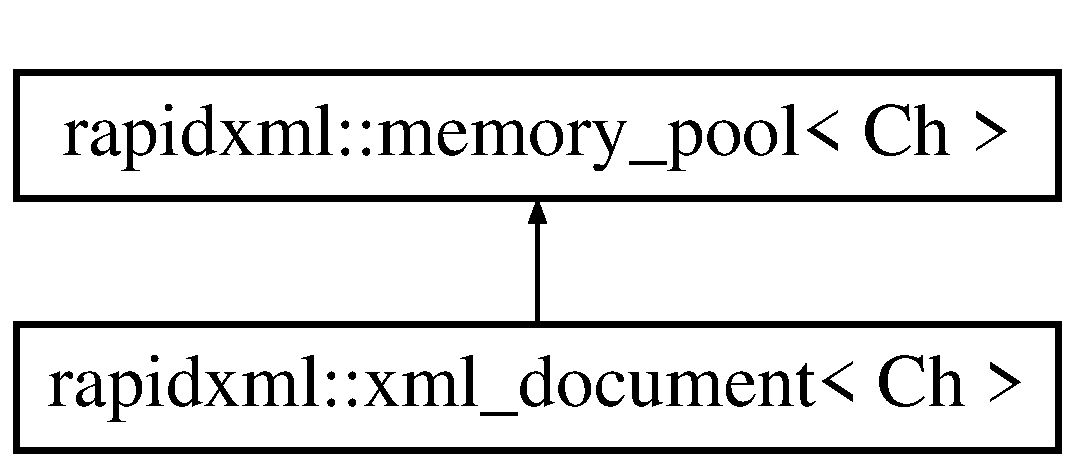
\includegraphics[height=2.000000cm]{classrapidxml_1_1memory__pool}
\end{center}
\end{figure}
\subsection*{Public Member Functions}
\begin{DoxyCompactItemize}
\item 
\hypertarget{classrapidxml_1_1memory__pool_a0b609da81dff28a19ebd704400788429}{\hyperlink{classrapidxml_1_1memory__pool_a0b609da81dff28a19ebd704400788429}{memory\-\_\-pool} ()}\label{classrapidxml_1_1memory__pool_a0b609da81dff28a19ebd704400788429}

\begin{DoxyCompactList}\small\item\em Constructs empty pool with default allocator functions. \end{DoxyCompactList}\item 
\hyperlink{classrapidxml_1_1memory__pool_a0a3e82126e59e4077f41e933130bb5a0}{$\sim$memory\-\_\-pool} ()
\item 
\hyperlink{classrapidxml_1_1xml__node}{xml\-\_\-node}$<$ Ch $>$ $\ast$ \hyperlink{classrapidxml_1_1memory__pool_a4118581c29ee9a2f6b55ebf7dac185f8}{allocate\-\_\-node} (node\-\_\-type type, const Ch $\ast$name=0, const Ch $\ast$value=0, std\-::size\-\_\-t name\-\_\-size=0, std\-::size\-\_\-t value\-\_\-size=0)
\item 
\hyperlink{classrapidxml_1_1xml__attribute}{xml\-\_\-attribute}$<$ Ch $>$ $\ast$ \hyperlink{classrapidxml_1_1memory__pool_a3de2a66c983336e006ea3844e244ed30}{allocate\-\_\-attribute} (const Ch $\ast$name=0, const Ch $\ast$value=0, std\-::size\-\_\-t name\-\_\-size=0, std\-::size\-\_\-t value\-\_\-size=0)
\item 
Ch $\ast$ \hyperlink{classrapidxml_1_1memory__pool_a171941b39d55b868358da97462185f58}{allocate\-\_\-string} (const Ch $\ast$source=0, std\-::size\-\_\-t size=0)
\item 
\hyperlink{classrapidxml_1_1xml__node}{xml\-\_\-node}$<$ Ch $>$ $\ast$ \hyperlink{classrapidxml_1_1memory__pool_a0a10679fc17597d339a0dc107f8a94ac}{clone\-\_\-node} (const \hyperlink{classrapidxml_1_1xml__node}{xml\-\_\-node}$<$ Ch $>$ $\ast$source, \hyperlink{classrapidxml_1_1xml__node}{xml\-\_\-node}$<$ Ch $>$ $\ast$result=0)
\item 
void \hyperlink{classrapidxml_1_1memory__pool_aad377c835fdaed1cb2cc9df194cf84e4}{clear} ()
\item 
void \hyperlink{classrapidxml_1_1memory__pool_a84d3d8d2cdfc00501e1dcf26d889ae03}{set\-\_\-allocator} (alloc\-\_\-func $\ast$af, free\-\_\-func $\ast$ff)
\end{DoxyCompactItemize}


\subsection{Detailed Description}
\subsubsection*{template$<$class Ch = char$>$class rapidxml\-::memory\-\_\-pool$<$ Ch $>$}

This class is used by the parser to create new nodes and attributes, without overheads of dynamic memory allocation. In most cases, you will not need to use this class directly. However, if you need to create nodes manually or modify names/values of nodes, you are encouraged to use \hyperlink{classrapidxml_1_1memory__pool}{memory\-\_\-pool} of relevant \hyperlink{classrapidxml_1_1xml__document}{xml\-\_\-document} to allocate the memory. Not only is this faster than allocating them by using {\ttfamily new} operator, but also their lifetime will be tied to the lifetime of document, possibly simplyfing memory management. \par
\par
 Call \hyperlink{classrapidxml_1_1memory__pool_a4118581c29ee9a2f6b55ebf7dac185f8}{allocate\-\_\-node()} or \hyperlink{classrapidxml_1_1memory__pool_a3de2a66c983336e006ea3844e244ed30}{allocate\-\_\-attribute()} functions to obtain new nodes or attributes from the pool. You can also call \hyperlink{classrapidxml_1_1memory__pool_a171941b39d55b868358da97462185f58}{allocate\-\_\-string()} function to allocate strings. Such strings can then be used as names or values of nodes without worrying about their lifetime. Note that there is no {\ttfamily free()} function -- all allocations are freed at once when \hyperlink{classrapidxml_1_1memory__pool_aad377c835fdaed1cb2cc9df194cf84e4}{clear()} function is called, or when the pool is destroyed. \par
\par
 It is also possible to create a standalone \hyperlink{classrapidxml_1_1memory__pool}{memory\-\_\-pool}, and use it to allocate nodes, whose lifetime will not be tied to any document. \par
\par
 Pool maintains {\ttfamily R\-A\-P\-I\-D\-X\-M\-L\-\_\-\-S\-T\-A\-T\-I\-C\-\_\-\-P\-O\-O\-L\-\_\-\-S\-I\-Z\-E} bytes of statically allocated memory. Until static memory is exhausted, no dynamic memory allocations are done. When static memory is exhausted, pool allocates additional blocks of memory of size {\ttfamily R\-A\-P\-I\-D\-X\-M\-L\-\_\-\-D\-Y\-N\-A\-M\-I\-C\-\_\-\-P\-O\-O\-L\-\_\-\-S\-I\-Z\-E} each, by using global {\ttfamily new\mbox{[}\mbox{]}} and {\ttfamily delete\mbox{[}\mbox{]}} operators. This behaviour can be changed by setting custom allocation routines. Use \hyperlink{classrapidxml_1_1memory__pool_a84d3d8d2cdfc00501e1dcf26d889ae03}{set\-\_\-allocator()} function to set them. \par
\par
 Allocations for nodes, attributes and strings are aligned at {\ttfamily R\-A\-P\-I\-D\-X\-M\-L\-\_\-\-A\-L\-I\-G\-N\-M\-E\-N\-T} bytes. This value defaults to the size of pointer on target architecture. \par
\par
 To obtain absolutely top performance from the parser, it is important that all nodes are allocated from a single, contiguous block of memory. Otherwise, cache misses when jumping between two (or more) disjoint blocks of memory can slow down parsing quite considerably. If required, you can tweak {\ttfamily R\-A\-P\-I\-D\-X\-M\-L\-\_\-\-S\-T\-A\-T\-I\-C\-\_\-\-P\-O\-O\-L\-\_\-\-S\-I\-Z\-E}, {\ttfamily R\-A\-P\-I\-D\-X\-M\-L\-\_\-\-D\-Y\-N\-A\-M\-I\-C\-\_\-\-P\-O\-O\-L\-\_\-\-S\-I\-Z\-E} and {\ttfamily R\-A\-P\-I\-D\-X\-M\-L\-\_\-\-A\-L\-I\-G\-N\-M\-E\-N\-T} to obtain best wasted memory to performance compromise. To do it, define their values before \hyperlink{rapidxml_8hpp}{rapidxml.\-hpp} file is included. 
\begin{DoxyParams}{Parameters}
{\em Ch} & Character type of created nodes. \\
\hline
\end{DoxyParams}


\subsection{Constructor \& Destructor Documentation}
\hypertarget{classrapidxml_1_1memory__pool_a0a3e82126e59e4077f41e933130bb5a0}{\index{rapidxml\-::memory\-\_\-pool@{rapidxml\-::memory\-\_\-pool}!$\sim$memory\-\_\-pool@{$\sim$memory\-\_\-pool}}
\index{$\sim$memory\-\_\-pool@{$\sim$memory\-\_\-pool}!rapidxml::memory_pool@{rapidxml\-::memory\-\_\-pool}}
\subsubsection[{$\sim$memory\-\_\-pool}]{\setlength{\rightskip}{0pt plus 5cm}template$<$class Ch  = char$>$ {\bf rapidxml\-::memory\-\_\-pool}$<$ Ch $>$\-::$\sim${\bf memory\-\_\-pool} (
\begin{DoxyParamCaption}
{}
\end{DoxyParamCaption}
)\hspace{0.3cm}{\ttfamily [inline]}}}\label{classrapidxml_1_1memory__pool_a0a3e82126e59e4077f41e933130bb5a0}
Destroys pool and frees all the memory. This causes memory occupied by nodes allocated by the pool to be freed. Nodes allocated from the pool are no longer valid. 

\subsection{Member Function Documentation}
\hypertarget{classrapidxml_1_1memory__pool_a3de2a66c983336e006ea3844e244ed30}{\index{rapidxml\-::memory\-\_\-pool@{rapidxml\-::memory\-\_\-pool}!allocate\-\_\-attribute@{allocate\-\_\-attribute}}
\index{allocate\-\_\-attribute@{allocate\-\_\-attribute}!rapidxml::memory_pool@{rapidxml\-::memory\-\_\-pool}}
\subsubsection[{allocate\-\_\-attribute}]{\setlength{\rightskip}{0pt plus 5cm}template$<$class Ch  = char$>$ {\bf xml\-\_\-attribute}$<$Ch$>$$\ast$ {\bf rapidxml\-::memory\-\_\-pool}$<$ Ch $>$\-::allocate\-\_\-attribute (
\begin{DoxyParamCaption}
\item[{const Ch $\ast$}]{name = {\ttfamily 0}, }
\item[{const Ch $\ast$}]{value = {\ttfamily 0}, }
\item[{std\-::size\-\_\-t}]{name\-\_\-size = {\ttfamily 0}, }
\item[{std\-::size\-\_\-t}]{value\-\_\-size = {\ttfamily 0}}
\end{DoxyParamCaption}
)\hspace{0.3cm}{\ttfamily [inline]}}}\label{classrapidxml_1_1memory__pool_a3de2a66c983336e006ea3844e244ed30}
Allocates a new attribute from the pool, and optionally assigns name and value to it. If the allocation request cannot be accomodated, this function will throw {\ttfamily std\-::bad\-\_\-alloc}. If exceptions are disabled by defining R\-A\-P\-I\-D\-X\-M\-L\-\_\-\-N\-O\-\_\-\-E\-X\-C\-E\-P\-T\-I\-O\-N\-S, this function will call rapidxml\-::parse\-\_\-error\-\_\-handler() function. 
\begin{DoxyParams}{Parameters}
{\em name} & Name to assign to the attribute, or 0 to assign no name. \\
\hline
{\em value} & Value to assign to the attribute, or 0 to assign no value. \\
\hline
{\em name\-\_\-size} & Size of name to assign, or 0 to automatically calculate size from name string. \\
\hline
{\em value\-\_\-size} & Size of value to assign, or 0 to automatically calculate size from value string. \\
\hline
\end{DoxyParams}
\begin{DoxyReturn}{Returns}
Pointer to allocated attribute. This pointer will never be N\-U\-L\-L. 
\end{DoxyReturn}
\hypertarget{classrapidxml_1_1memory__pool_a4118581c29ee9a2f6b55ebf7dac185f8}{\index{rapidxml\-::memory\-\_\-pool@{rapidxml\-::memory\-\_\-pool}!allocate\-\_\-node@{allocate\-\_\-node}}
\index{allocate\-\_\-node@{allocate\-\_\-node}!rapidxml::memory_pool@{rapidxml\-::memory\-\_\-pool}}
\subsubsection[{allocate\-\_\-node}]{\setlength{\rightskip}{0pt plus 5cm}template$<$class Ch  = char$>$ {\bf xml\-\_\-node}$<$Ch$>$$\ast$ {\bf rapidxml\-::memory\-\_\-pool}$<$ Ch $>$\-::allocate\-\_\-node (
\begin{DoxyParamCaption}
\item[{node\-\_\-type}]{type, }
\item[{const Ch $\ast$}]{name = {\ttfamily 0}, }
\item[{const Ch $\ast$}]{value = {\ttfamily 0}, }
\item[{std\-::size\-\_\-t}]{name\-\_\-size = {\ttfamily 0}, }
\item[{std\-::size\-\_\-t}]{value\-\_\-size = {\ttfamily 0}}
\end{DoxyParamCaption}
)\hspace{0.3cm}{\ttfamily [inline]}}}\label{classrapidxml_1_1memory__pool_a4118581c29ee9a2f6b55ebf7dac185f8}
Allocates a new node from the pool, and optionally assigns name and value to it. If the allocation request cannot be accomodated, this function will throw {\ttfamily std\-::bad\-\_\-alloc}. If exceptions are disabled by defining R\-A\-P\-I\-D\-X\-M\-L\-\_\-\-N\-O\-\_\-\-E\-X\-C\-E\-P\-T\-I\-O\-N\-S, this function will call rapidxml\-::parse\-\_\-error\-\_\-handler() function. 
\begin{DoxyParams}{Parameters}
{\em type} & Type of node to create. \\
\hline
{\em name} & Name to assign to the node, or 0 to assign no name. \\
\hline
{\em value} & Value to assign to the node, or 0 to assign no value. \\
\hline
{\em name\-\_\-size} & Size of name to assign, or 0 to automatically calculate size from name string. \\
\hline
{\em value\-\_\-size} & Size of value to assign, or 0 to automatically calculate size from value string. \\
\hline
\end{DoxyParams}
\begin{DoxyReturn}{Returns}
Pointer to allocated node. This pointer will never be N\-U\-L\-L. 
\end{DoxyReturn}
\hypertarget{classrapidxml_1_1memory__pool_a171941b39d55b868358da97462185f58}{\index{rapidxml\-::memory\-\_\-pool@{rapidxml\-::memory\-\_\-pool}!allocate\-\_\-string@{allocate\-\_\-string}}
\index{allocate\-\_\-string@{allocate\-\_\-string}!rapidxml::memory_pool@{rapidxml\-::memory\-\_\-pool}}
\subsubsection[{allocate\-\_\-string}]{\setlength{\rightskip}{0pt plus 5cm}template$<$class Ch  = char$>$ Ch$\ast$ {\bf rapidxml\-::memory\-\_\-pool}$<$ Ch $>$\-::allocate\-\_\-string (
\begin{DoxyParamCaption}
\item[{const Ch $\ast$}]{source = {\ttfamily 0}, }
\item[{std\-::size\-\_\-t}]{size = {\ttfamily 0}}
\end{DoxyParamCaption}
)\hspace{0.3cm}{\ttfamily [inline]}}}\label{classrapidxml_1_1memory__pool_a171941b39d55b868358da97462185f58}
Allocates a char array of given size from the pool, and optionally copies a given string to it. If the allocation request cannot be accomodated, this function will throw {\ttfamily std\-::bad\-\_\-alloc}. If exceptions are disabled by defining R\-A\-P\-I\-D\-X\-M\-L\-\_\-\-N\-O\-\_\-\-E\-X\-C\-E\-P\-T\-I\-O\-N\-S, this function will call rapidxml\-::parse\-\_\-error\-\_\-handler() function. 
\begin{DoxyParams}{Parameters}
{\em source} & String to initialize the allocated memory with, or 0 to not initialize it. \\
\hline
{\em size} & Number of characters to allocate, or zero to calculate it automatically from source string length; if size is 0, source string must be specified and null terminated. \\
\hline
\end{DoxyParams}
\begin{DoxyReturn}{Returns}
Pointer to allocated char array. This pointer will never be N\-U\-L\-L. 
\end{DoxyReturn}
\hypertarget{classrapidxml_1_1memory__pool_aad377c835fdaed1cb2cc9df194cf84e4}{\index{rapidxml\-::memory\-\_\-pool@{rapidxml\-::memory\-\_\-pool}!clear@{clear}}
\index{clear@{clear}!rapidxml::memory_pool@{rapidxml\-::memory\-\_\-pool}}
\subsubsection[{clear}]{\setlength{\rightskip}{0pt plus 5cm}template$<$class Ch  = char$>$ void {\bf rapidxml\-::memory\-\_\-pool}$<$ Ch $>$\-::clear (
\begin{DoxyParamCaption}
{}
\end{DoxyParamCaption}
)\hspace{0.3cm}{\ttfamily [inline]}}}\label{classrapidxml_1_1memory__pool_aad377c835fdaed1cb2cc9df194cf84e4}
Clears the pool. This causes memory occupied by nodes allocated by the pool to be freed. Any nodes or strings allocated from the pool will no longer be valid. \hypertarget{classrapidxml_1_1memory__pool_a0a10679fc17597d339a0dc107f8a94ac}{\index{rapidxml\-::memory\-\_\-pool@{rapidxml\-::memory\-\_\-pool}!clone\-\_\-node@{clone\-\_\-node}}
\index{clone\-\_\-node@{clone\-\_\-node}!rapidxml::memory_pool@{rapidxml\-::memory\-\_\-pool}}
\subsubsection[{clone\-\_\-node}]{\setlength{\rightskip}{0pt plus 5cm}template$<$class Ch  = char$>$ {\bf xml\-\_\-node}$<$Ch$>$$\ast$ {\bf rapidxml\-::memory\-\_\-pool}$<$ Ch $>$\-::clone\-\_\-node (
\begin{DoxyParamCaption}
\item[{const {\bf xml\-\_\-node}$<$ Ch $>$ $\ast$}]{source, }
\item[{{\bf xml\-\_\-node}$<$ Ch $>$ $\ast$}]{result = {\ttfamily 0}}
\end{DoxyParamCaption}
)\hspace{0.3cm}{\ttfamily [inline]}}}\label{classrapidxml_1_1memory__pool_a0a10679fc17597d339a0dc107f8a94ac}
Clones an \hyperlink{classrapidxml_1_1xml__node}{xml\-\_\-node} and its hierarchy of child nodes and attributes. Nodes and attributes are allocated from this memory pool. Names and values are not cloned, they are shared between the clone and the source. Result node can be optionally specified as a second parameter, in which case its contents will be replaced with cloned source node. This is useful when you want to clone entire document. 
\begin{DoxyParams}{Parameters}
{\em source} & Node to clone. \\
\hline
{\em result} & Node to put results in, or 0 to automatically allocate result node \\
\hline
\end{DoxyParams}
\begin{DoxyReturn}{Returns}
Pointer to cloned node. This pointer will never be N\-U\-L\-L. 
\end{DoxyReturn}
\hypertarget{classrapidxml_1_1memory__pool_a84d3d8d2cdfc00501e1dcf26d889ae03}{\index{rapidxml\-::memory\-\_\-pool@{rapidxml\-::memory\-\_\-pool}!set\-\_\-allocator@{set\-\_\-allocator}}
\index{set\-\_\-allocator@{set\-\_\-allocator}!rapidxml::memory_pool@{rapidxml\-::memory\-\_\-pool}}
\subsubsection[{set\-\_\-allocator}]{\setlength{\rightskip}{0pt plus 5cm}template$<$class Ch  = char$>$ void {\bf rapidxml\-::memory\-\_\-pool}$<$ Ch $>$\-::set\-\_\-allocator (
\begin{DoxyParamCaption}
\item[{alloc\-\_\-func $\ast$}]{af, }
\item[{free\-\_\-func $\ast$}]{ff}
\end{DoxyParamCaption}
)\hspace{0.3cm}{\ttfamily [inline]}}}\label{classrapidxml_1_1memory__pool_a84d3d8d2cdfc00501e1dcf26d889ae03}
Sets or resets the user-\/defined memory allocation functions for the pool. This can only be called when no memory is allocated from the pool yet, otherwise results are undefined. Allocation function must not return invalid pointer on failure. It should either throw, stop the program, or use {\ttfamily longjmp()} function to pass control to other place of program. If it returns invalid pointer, results are undefined. \par
\par
 User defined allocation functions must have the following forms\-: \par
{\ttfamily  \par
void $\ast$allocate(std\-::size\-\_\-t size); \par
void free(void $\ast$pointer); }\par
 
\begin{DoxyParams}{Parameters}
{\em af} & Allocation function, or 0 to restore default function \\
\hline
{\em ff} & Free function, or 0 to restore default function \\
\hline
\end{DoxyParams}


The documentation for this class was generated from the following file\-:\begin{DoxyCompactItemize}
\item 
\hyperlink{rapidxml_8hpp}{rapidxml.\-hpp}\end{DoxyCompactItemize}

\hypertarget{structstrtk_1_1multiple__char__delimiter__predicate}{\section{strtk\-:\-:multiple\-\_\-char\-\_\-delimiter\-\_\-predicate Struct Reference}
\label{structstrtk_1_1multiple__char__delimiter__predicate}\index{strtk\-::multiple\-\_\-char\-\_\-delimiter\-\_\-predicate@{strtk\-::multiple\-\_\-char\-\_\-delimiter\-\_\-predicate}}
}
\subsection*{Public Member Functions}
\begin{DoxyCompactItemize}
\item 
\hypertarget{structstrtk_1_1multiple__char__delimiter__predicate_a6634d2440b9806c2f4f1b404eead662a}{{\footnotesize template$<$typename Iterator $>$ }\\{\bfseries multiple\-\_\-char\-\_\-delimiter\-\_\-predicate} (const Iterator begin, const Iterator end)}\label{structstrtk_1_1multiple__char__delimiter__predicate_a6634d2440b9806c2f4f1b404eead662a}

\item 
\hypertarget{structstrtk_1_1multiple__char__delimiter__predicate_a60d12458ad94f22b7b2209f21b43b4ee}{{\bfseries multiple\-\_\-char\-\_\-delimiter\-\_\-predicate} (const std\-::string \&s)}\label{structstrtk_1_1multiple__char__delimiter__predicate_a60d12458ad94f22b7b2209f21b43b4ee}

\item 
\hypertarget{structstrtk_1_1multiple__char__delimiter__predicate_a43781593a6e76d8251dc0d5aefbce843}{bool {\bfseries operator()} (const unsigned char \&c) const }\label{structstrtk_1_1multiple__char__delimiter__predicate_a43781593a6e76d8251dc0d5aefbce843}

\item 
\hypertarget{structstrtk_1_1multiple__char__delimiter__predicate_ad8d5d933432ea3d2c02572e2ae6590b5}{bool {\bfseries operator()} (const char \&c) const }\label{structstrtk_1_1multiple__char__delimiter__predicate_ad8d5d933432ea3d2c02572e2ae6590b5}

\end{DoxyCompactItemize}


The documentation for this struct was generated from the following file\-:\begin{DoxyCompactItemize}
\item 
strtk.\-hpp\end{DoxyCompactItemize}

\hypertarget{structstrtk_1_1multiple__delimiter__predicate}{\section{strtk\-:\-:multiple\-\_\-delimiter\-\_\-predicate$<$ T $>$ Struct Template Reference}
\label{structstrtk_1_1multiple__delimiter__predicate}\index{strtk\-::multiple\-\_\-delimiter\-\_\-predicate$<$ T $>$@{strtk\-::multiple\-\_\-delimiter\-\_\-predicate$<$ T $>$}}
}
\subsection*{Public Types}
\begin{DoxyCompactItemize}
\item 
\hypertarget{structstrtk_1_1multiple__delimiter__predicate_a6855480d884e88fb8add8b46a8a2b952}{typedef T {\bfseries value\-\_\-type}}\label{structstrtk_1_1multiple__delimiter__predicate_a6855480d884e88fb8add8b46a8a2b952}

\end{DoxyCompactItemize}
\subsection*{Public Member Functions}
\begin{DoxyCompactItemize}
\item 
\hypertarget{structstrtk_1_1multiple__delimiter__predicate_abd62516a0d3ca46cbd209635cb0e4947}{{\bfseries multiple\-\_\-delimiter\-\_\-predicate} (const T $\ast$d\-\_\-begin, const T $\ast$d\-\_\-end)}\label{structstrtk_1_1multiple__delimiter__predicate_abd62516a0d3ca46cbd209635cb0e4947}

\item 
\hypertarget{structstrtk_1_1multiple__delimiter__predicate_a675f0597a53567f11e86a7a56c1b5697}{{\bfseries multiple\-\_\-delimiter\-\_\-predicate} (const T d\mbox{[}$\,$\mbox{]}, const std\-::size\-\_\-t \&length)}\label{structstrtk_1_1multiple__delimiter__predicate_a675f0597a53567f11e86a7a56c1b5697}

\item 
\hypertarget{structstrtk_1_1multiple__delimiter__predicate_a124afad80327733e3245fd0c5b2016e1}{{\footnotesize template$<$typename Iterator $>$ }\\{\bfseries multiple\-\_\-delimiter\-\_\-predicate} (const Iterator begin, const Iterator end)}\label{structstrtk_1_1multiple__delimiter__predicate_a124afad80327733e3245fd0c5b2016e1}

\item 
\hypertarget{structstrtk_1_1multiple__delimiter__predicate_ad0a809ad2e33b992cfa84785ae2fed4f}{{\footnotesize template$<$typename Type $>$ }\\{\bfseries multiple\-\_\-delimiter\-\_\-predicate} (const \hyperlink{classstrtk_1_1range_1_1adapter}{range\-::adapter}$<$ Type $>$ \&r)}\label{structstrtk_1_1multiple__delimiter__predicate_ad0a809ad2e33b992cfa84785ae2fed4f}

\item 
\hypertarget{structstrtk_1_1multiple__delimiter__predicate_af18033cefb0481b0957ecc49390cf08c}{bool {\bfseries operator()} (const T \&d) const }\label{structstrtk_1_1multiple__delimiter__predicate_af18033cefb0481b0957ecc49390cf08c}

\end{DoxyCompactItemize}


The documentation for this struct was generated from the following file\-:\begin{DoxyCompactItemize}
\item 
strtk.\-hpp\end{DoxyCompactItemize}

\hypertarget{structstrtk_1_1multiset__sink}{\section{strtk\-:\-:multiset\-\_\-sink$<$ T $>$ Struct Template Reference}
\label{structstrtk_1_1multiset__sink}\index{strtk\-::multiset\-\_\-sink$<$ T $>$@{strtk\-::multiset\-\_\-sink$<$ T $>$}}
}
\subsection*{Public Types}
\begin{DoxyCompactItemize}
\item 
\hypertarget{structstrtk_1_1multiset__sink_a8e6d9a502c3d15c46b48804ea2d3d0f4}{typedef \hyperlink{classstrtk_1_1sink__type}{sink\-\_\-type}\\*
$<$ std\-::multiset$<$ T $>$ $>$ {\bfseries type}}\label{structstrtk_1_1multiset__sink_a8e6d9a502c3d15c46b48804ea2d3d0f4}

\end{DoxyCompactItemize}


The documentation for this struct was generated from the following file\-:\begin{DoxyCompactItemize}
\item 
strtk.\-hpp\end{DoxyCompactItemize}

\hypertarget{structstrtk_1_1details_1_1next__size}{\section{strtk\-:\-:details\-:\-:next\-\_\-size$<$ N $>$ Struct Template Reference}
\label{structstrtk_1_1details_1_1next__size}\index{strtk\-::details\-::next\-\_\-size$<$ N $>$@{strtk\-::details\-::next\-\_\-size$<$ N $>$}}
}
\subsection*{Public Types}
\begin{DoxyCompactItemize}
\item 
enum \{ {\bfseries size} = (N $>$= 8) ? 8 \-: ((N $>$= 4) ? 4 \-: ((N $>$= 2) ? 2 \-: 1))
 \}
\end{DoxyCompactItemize}


The documentation for this struct was generated from the following file\-:\begin{DoxyCompactItemize}
\item 
strtk.\-hpp\end{DoxyCompactItemize}

\hypertarget{structstrtk_1_1keyvalue_1_1details_1_1no__op__validator}{\section{strtk\-:\-:keyvalue\-:\-:details\-:\-:no\-\_\-op\-\_\-validator Struct Reference}
\label{structstrtk_1_1keyvalue_1_1details_1_1no__op__validator}\index{strtk\-::keyvalue\-::details\-::no\-\_\-op\-\_\-validator@{strtk\-::keyvalue\-::details\-::no\-\_\-op\-\_\-validator}}
}
\subsection*{Public Member Functions}
\begin{DoxyCompactItemize}
\item 
\hypertarget{structstrtk_1_1keyvalue_1_1details_1_1no__op__validator_a02484c668dcc580d0edc20a6c0284211}{{\footnotesize template$<$typename Range $>$ }\\bool {\bfseries operator()} (const Range \&)}\label{structstrtk_1_1keyvalue_1_1details_1_1no__op__validator_a02484c668dcc580d0edc20a6c0284211}

\end{DoxyCompactItemize}


The documentation for this struct was generated from the following file\-:\begin{DoxyCompactItemize}
\item 
strtk.\-hpp\end{DoxyCompactItemize}

\hypertarget{structstrtk_1_1details_1_1no__t}{\section{strtk\-:\-:details\-:\-:no\-\_\-t Struct Reference}
\label{structstrtk_1_1details_1_1no__t}\index{strtk\-::details\-::no\-\_\-t@{strtk\-::details\-::no\-\_\-t}}
}


The documentation for this struct was generated from the following file\-:\begin{DoxyCompactItemize}
\item 
strtk.\-hpp\end{DoxyCompactItemize}

\hypertarget{classrapidxml_1_1node__iterator}{\section{rapidxml\-:\-:node\-\_\-iterator$<$ Ch $>$ Class Template Reference}
\label{classrapidxml_1_1node__iterator}\index{rapidxml\-::node\-\_\-iterator$<$ Ch $>$@{rapidxml\-::node\-\_\-iterator$<$ Ch $>$}}
}


Iterator of child nodes of \hyperlink{classrapidxml_1_1xml__node}{xml\-\_\-node}.  




{\ttfamily \#include $<$rapidxml\-\_\-iterators.\-hpp$>$}

\subsection*{Public Types}
\begin{DoxyCompactItemize}
\item 
\hypertarget{classrapidxml_1_1node__iterator_ade6310119ed1f72c94830e006fac69b7}{typedef \hyperlink{classrapidxml_1_1xml__node}{xml\-\_\-node}$<$ Ch $>$ {\bfseries value\-\_\-type}}\label{classrapidxml_1_1node__iterator_ade6310119ed1f72c94830e006fac69b7}

\item 
\hypertarget{classrapidxml_1_1node__iterator_ad7fabbcb7d3d9e4e220299c5475b9e9c}{typedef \hyperlink{classrapidxml_1_1xml__node}{xml\-\_\-node}$<$ Ch $>$ \& {\bfseries reference}}\label{classrapidxml_1_1node__iterator_ad7fabbcb7d3d9e4e220299c5475b9e9c}

\item 
\hypertarget{classrapidxml_1_1node__iterator_a65dca8bca2b9c29f635b9ad0bdeeecb9}{typedef \hyperlink{classrapidxml_1_1xml__node}{xml\-\_\-node}$<$ Ch $>$ $\ast$ {\bfseries pointer}}\label{classrapidxml_1_1node__iterator_a65dca8bca2b9c29f635b9ad0bdeeecb9}

\item 
\hypertarget{classrapidxml_1_1node__iterator_a5bdc462b980a52c5fa2d99ac9f4f4bff}{typedef std\-::ptrdiff\-\_\-t {\bfseries difference\-\_\-type}}\label{classrapidxml_1_1node__iterator_a5bdc462b980a52c5fa2d99ac9f4f4bff}

\item 
\hypertarget{classrapidxml_1_1node__iterator_a8e82d75f768e17bf7349d010ee26c037}{typedef \\*
std\-::bidirectional\-\_\-iterator\-\_\-tag {\bfseries iterator\-\_\-category}}\label{classrapidxml_1_1node__iterator_a8e82d75f768e17bf7349d010ee26c037}

\end{DoxyCompactItemize}
\subsection*{Public Member Functions}
\begin{DoxyCompactItemize}
\item 
\hypertarget{classrapidxml_1_1node__iterator_a94c3da59b54e4bd003e226cc35b3c266}{{\bfseries node\-\_\-iterator} (\hyperlink{classrapidxml_1_1xml__node}{xml\-\_\-node}$<$ Ch $>$ $\ast$node)}\label{classrapidxml_1_1node__iterator_a94c3da59b54e4bd003e226cc35b3c266}

\item 
\hypertarget{classrapidxml_1_1node__iterator_ab31fe5bc1fd01fee8a2b31c3e42d78ed}{\hyperlink{classrapidxml_1_1xml__node}{reference} {\bfseries operator$\ast$} () const }\label{classrapidxml_1_1node__iterator_ab31fe5bc1fd01fee8a2b31c3e42d78ed}

\item 
\hypertarget{classrapidxml_1_1node__iterator_a9b3e7d58c4a628524914932e0663ddfb}{\hyperlink{classrapidxml_1_1xml__node}{pointer} {\bfseries operator-\/$>$} () const }\label{classrapidxml_1_1node__iterator_a9b3e7d58c4a628524914932e0663ddfb}

\item 
\hypertarget{classrapidxml_1_1node__iterator_a8d6b184a76b2ec8a8b5e90bc013c80ed}{\hyperlink{classrapidxml_1_1node__iterator}{node\-\_\-iterator} \& {\bfseries operator++} ()}\label{classrapidxml_1_1node__iterator_a8d6b184a76b2ec8a8b5e90bc013c80ed}

\item 
\hypertarget{classrapidxml_1_1node__iterator_ad01b4e43e348a330984833fd4924d0f2}{\hyperlink{classrapidxml_1_1node__iterator}{node\-\_\-iterator} {\bfseries operator++} (int)}\label{classrapidxml_1_1node__iterator_ad01b4e43e348a330984833fd4924d0f2}

\item 
\hypertarget{classrapidxml_1_1node__iterator_ace52107ecd1bcf02e49619e86206e3a3}{\hyperlink{classrapidxml_1_1node__iterator}{node\-\_\-iterator} \& {\bfseries operator-\/-\/} ()}\label{classrapidxml_1_1node__iterator_ace52107ecd1bcf02e49619e86206e3a3}

\item 
\hypertarget{classrapidxml_1_1node__iterator_a4ca35716bb7865f199a137b063af6080}{\hyperlink{classrapidxml_1_1node__iterator}{node\-\_\-iterator} {\bfseries operator-\/-\/} (int)}\label{classrapidxml_1_1node__iterator_a4ca35716bb7865f199a137b063af6080}

\item 
\hypertarget{classrapidxml_1_1node__iterator_a5cb8a3b0d65a1a2517995e986a4debfd}{bool {\bfseries operator==} (const \hyperlink{classrapidxml_1_1node__iterator}{node\-\_\-iterator}$<$ Ch $>$ \&rhs)}\label{classrapidxml_1_1node__iterator_a5cb8a3b0d65a1a2517995e986a4debfd}

\item 
\hypertarget{classrapidxml_1_1node__iterator_a20f1e25347d7e3856694f18597f7c8e2}{bool {\bfseries operator!=} (const \hyperlink{classrapidxml_1_1node__iterator}{node\-\_\-iterator}$<$ Ch $>$ \&rhs)}\label{classrapidxml_1_1node__iterator_a20f1e25347d7e3856694f18597f7c8e2}

\end{DoxyCompactItemize}


\subsection{Detailed Description}
\subsubsection*{template$<$class Ch$>$class rapidxml\-::node\-\_\-iterator$<$ Ch $>$}

Iterator of child nodes of \hyperlink{classrapidxml_1_1xml__node}{xml\-\_\-node}. 

The documentation for this class was generated from the following file\-:\begin{DoxyCompactItemize}
\item 
\hyperlink{rapidxml__iterators_8hpp}{rapidxml\-\_\-iterators.\-hpp}\end{DoxyCompactItemize}

\hypertarget{structstrtk_1_1nonempty__range}{\section{strtk\-:\-:nonempty\-\_\-range Struct Reference}
\label{structstrtk_1_1nonempty__range}\index{strtk\-::nonempty\-\_\-range@{strtk\-::nonempty\-\_\-range}}
}
\subsection*{Public Member Functions}
\begin{DoxyCompactItemize}
\item 
\hypertarget{structstrtk_1_1nonempty__range_ad469236b6d5583d3acc92a6a297b0eb8}{{\footnotesize template$<$typename Input\-Iterator $>$ }\\bool {\bfseries operator()} (const Input\-Iterator begin, const Input\-Iterator end)}\label{structstrtk_1_1nonempty__range_ad469236b6d5583d3acc92a6a297b0eb8}

\end{DoxyCompactItemize}


The documentation for this struct was generated from the following file\-:\begin{DoxyCompactItemize}
\item 
strtk.\-hpp\end{DoxyCompactItemize}

\hypertarget{structstrtk_1_1details_1_1not__supported__type__tag}{\section{strtk\-:\-:details\-:\-:not\-\_\-supported\-\_\-type\-\_\-tag Struct Reference}
\label{structstrtk_1_1details_1_1not__supported__type__tag}\index{strtk\-::details\-::not\-\_\-supported\-\_\-type\-\_\-tag@{strtk\-::details\-::not\-\_\-supported\-\_\-type\-\_\-tag}}
}


The documentation for this struct was generated from the following file\-:\begin{DoxyCompactItemize}
\item 
strtk.\-hpp\end{DoxyCompactItemize}

\hypertarget{structstrtk_1_1details_1_1numeric}{\section{strtk\-:\-:details\-:\-:numeric$<$ T $>$ Struct Template Reference}
\label{structstrtk_1_1details_1_1numeric}\index{strtk\-::details\-::numeric$<$ T $>$@{strtk\-::details\-::numeric$<$ T $>$}}
}


The documentation for this struct was generated from the following file\-:\begin{DoxyCompactItemize}
\item 
strtk.\-hpp\end{DoxyCompactItemize}

\hypertarget{structstrtk_1_1details_1_1numeric_3_01double_01_4}{\section{strtk\-:\-:details\-:\-:numeric$<$ double $>$ Struct Template Reference}
\label{structstrtk_1_1details_1_1numeric_3_01double_01_4}\index{strtk\-::details\-::numeric$<$ double $>$@{strtk\-::details\-::numeric$<$ double $>$}}
}
\subsection*{Public Types}
\begin{DoxyCompactItemize}
\item 
enum \{ {\bfseries min\-\_\-exp} = -\/307, 
{\bfseries max\-\_\-exp} = +308, 
{\bfseries precision} = 15
 \}
\end{DoxyCompactItemize}


The documentation for this struct was generated from the following file\-:\begin{DoxyCompactItemize}
\item 
strtk.\-hpp\end{DoxyCompactItemize}

\hypertarget{structstrtk_1_1details_1_1numeric_3_01float_01_4}{\section{strtk\-:\-:details\-:\-:numeric$<$ float $>$ Struct Template Reference}
\label{structstrtk_1_1details_1_1numeric_3_01float_01_4}\index{strtk\-::details\-::numeric$<$ float $>$@{strtk\-::details\-::numeric$<$ float $>$}}
}
\subsection*{Public Types}
\begin{DoxyCompactItemize}
\item 
enum \{ {\bfseries min\-\_\-exp} = -\/37, 
{\bfseries max\-\_\-exp} = +38, 
{\bfseries precision} = 10
 \}
\end{DoxyCompactItemize}


The documentation for this struct was generated from the following file\-:\begin{DoxyCompactItemize}
\item 
strtk.\-hpp\end{DoxyCompactItemize}

\hypertarget{structstrtk_1_1details_1_1numeric_3_01int_01_4}{\section{strtk\-:\-:details\-:\-:numeric$<$ int $>$ Struct Template Reference}
\label{structstrtk_1_1details_1_1numeric_3_01int_01_4}\index{strtk\-::details\-::numeric$<$ int $>$@{strtk\-::details\-::numeric$<$ int $>$}}
}
\subsection*{Static Public Attributes}
\begin{DoxyCompactItemize}
\item 
\hypertarget{structstrtk_1_1details_1_1numeric_3_01int_01_4_a1c72ff10531397701480e0aaec7dd821}{static const unsigned int {\bfseries length} = 10}\label{structstrtk_1_1details_1_1numeric_3_01int_01_4_a1c72ff10531397701480e0aaec7dd821}

\item 
\hypertarget{structstrtk_1_1details_1_1numeric_3_01int_01_4_a4e16b5c73d916deb6893cd071fd0ac98}{static const unsigned int {\bfseries size} = 16}\label{structstrtk_1_1details_1_1numeric_3_01int_01_4_a4e16b5c73d916deb6893cd071fd0ac98}

\item 
\hypertarget{structstrtk_1_1details_1_1numeric_3_01int_01_4_ae82cf86e97e0ba1e5ec619bd84506b6e}{static const unsigned int {\bfseries bound\-\_\-length} = 10}\label{structstrtk_1_1details_1_1numeric_3_01int_01_4_ae82cf86e97e0ba1e5ec619bd84506b6e}

\item 
\hypertarget{structstrtk_1_1details_1_1numeric_3_01int_01_4_ad185de4c8579c64113d45ad686022020}{static const int {\bfseries m10} = 214748364}\label{structstrtk_1_1details_1_1numeric_3_01int_01_4_ad185de4c8579c64113d45ad686022020}

\item 
\hypertarget{structstrtk_1_1details_1_1numeric_3_01int_01_4_a60c642905cb4b802a64386d1e7a89e28}{static const int {\bfseries ldpos} = 7}\label{structstrtk_1_1details_1_1numeric_3_01int_01_4_a60c642905cb4b802a64386d1e7a89e28}

\item 
\hypertarget{structstrtk_1_1details_1_1numeric_3_01int_01_4_a85d9607694fd371e035587ad274534f3}{static const int {\bfseries ldneg} = 8}\label{structstrtk_1_1details_1_1numeric_3_01int_01_4_a85d9607694fd371e035587ad274534f3}

\end{DoxyCompactItemize}


The documentation for this struct was generated from the following file\-:\begin{DoxyCompactItemize}
\item 
strtk.\-hpp\end{DoxyCompactItemize}

\hypertarget{structstrtk_1_1details_1_1numeric_3_01long_01_4}{\section{strtk\-:\-:details\-:\-:numeric$<$ long $>$ Struct Template Reference}
\label{structstrtk_1_1details_1_1numeric_3_01long_01_4}\index{strtk\-::details\-::numeric$<$ long $>$@{strtk\-::details\-::numeric$<$ long $>$}}
}
\subsection*{Static Public Attributes}
\begin{DoxyCompactItemize}
\item 
\hypertarget{structstrtk_1_1details_1_1numeric_3_01long_01_4_a23939ffd0ab6dcec95308a31cb65d14b}{static const unsigned int {\bfseries length} = 10}\label{structstrtk_1_1details_1_1numeric_3_01long_01_4_a23939ffd0ab6dcec95308a31cb65d14b}

\item 
\hypertarget{structstrtk_1_1details_1_1numeric_3_01long_01_4_acae0abc750d81b77508b4a88d3feeffd}{static const unsigned int {\bfseries size} = 16}\label{structstrtk_1_1details_1_1numeric_3_01long_01_4_acae0abc750d81b77508b4a88d3feeffd}

\item 
\hypertarget{structstrtk_1_1details_1_1numeric_3_01long_01_4_a1effbcf9649348954ab732921f372cc0}{static const unsigned int {\bfseries bound\-\_\-length} = 10}\label{structstrtk_1_1details_1_1numeric_3_01long_01_4_a1effbcf9649348954ab732921f372cc0}

\item 
\hypertarget{structstrtk_1_1details_1_1numeric_3_01long_01_4_ac52a7fd84c8359ef5107fabc2114888e}{static const long {\bfseries m10} = 214748364}\label{structstrtk_1_1details_1_1numeric_3_01long_01_4_ac52a7fd84c8359ef5107fabc2114888e}

\item 
\hypertarget{structstrtk_1_1details_1_1numeric_3_01long_01_4_a38ce1ed26dc80c1b62b00c8be0ebc382}{static const long {\bfseries ldpos} = 7}\label{structstrtk_1_1details_1_1numeric_3_01long_01_4_a38ce1ed26dc80c1b62b00c8be0ebc382}

\item 
\hypertarget{structstrtk_1_1details_1_1numeric_3_01long_01_4_af0d8fbe9434b50251a77cd3bd21f0eb6}{static const long {\bfseries ldneg} = 8}\label{structstrtk_1_1details_1_1numeric_3_01long_01_4_af0d8fbe9434b50251a77cd3bd21f0eb6}

\end{DoxyCompactItemize}


The documentation for this struct was generated from the following file\-:\begin{DoxyCompactItemize}
\item 
strtk.\-hpp\end{DoxyCompactItemize}

\hypertarget{structstrtk_1_1details_1_1numeric_3_01long_01double_01_4}{\section{strtk\-:\-:details\-:\-:numeric$<$ long double $>$ Struct Template Reference}
\label{structstrtk_1_1details_1_1numeric_3_01long_01double_01_4}\index{strtk\-::details\-::numeric$<$ long double $>$@{strtk\-::details\-::numeric$<$ long double $>$}}
}
\subsection*{Public Types}
\begin{DoxyCompactItemize}
\item 
enum \{ {\bfseries min\-\_\-exp} = ld\-:\-:i, 
{\bfseries max\-\_\-exp} = ld\-:\-:a, 
{\bfseries precision} = ld\-:\-:p
 \}
\item 
\hypertarget{structstrtk_1_1details_1_1numeric_3_01long_01double_01_4_a6ada7ea6d37ad505b67b7d8e2cef0391}{typedef \hyperlink{structstrtk_1_1details_1_1ldt}{ldt}$<$ long double, \\*
sizeof(long double)$>$ {\bfseries ld}}\label{structstrtk_1_1details_1_1numeric_3_01long_01double_01_4_a6ada7ea6d37ad505b67b7d8e2cef0391}

\end{DoxyCompactItemize}


The documentation for this struct was generated from the following file\-:\begin{DoxyCompactItemize}
\item 
strtk.\-hpp\end{DoxyCompactItemize}

\hypertarget{structstrtk_1_1details_1_1numeric_3_01long_01long_01_4}{\section{strtk\-:\-:details\-:\-:numeric$<$ long long $>$ Struct Template Reference}
\label{structstrtk_1_1details_1_1numeric_3_01long_01long_01_4}\index{strtk\-::details\-::numeric$<$ long long $>$@{strtk\-::details\-::numeric$<$ long long $>$}}
}
\subsection*{Static Public Attributes}
\begin{DoxyCompactItemize}
\item 
\hypertarget{structstrtk_1_1details_1_1numeric_3_01long_01long_01_4_a6a9c903712e8c639dc8433748c9b97dc}{static const unsigned int {\bfseries length} = 19}\label{structstrtk_1_1details_1_1numeric_3_01long_01long_01_4_a6a9c903712e8c639dc8433748c9b97dc}

\item 
\hypertarget{structstrtk_1_1details_1_1numeric_3_01long_01long_01_4_a8e57afeea651e2fa7e692b8097f63b96}{static const unsigned int {\bfseries size} = 24}\label{structstrtk_1_1details_1_1numeric_3_01long_01long_01_4_a8e57afeea651e2fa7e692b8097f63b96}

\item 
\hypertarget{structstrtk_1_1details_1_1numeric_3_01long_01long_01_4_a05e6ec6420de61f8a74e6f7eaa0b7b98}{static const unsigned int {\bfseries bound\-\_\-length} = 19}\label{structstrtk_1_1details_1_1numeric_3_01long_01long_01_4_a05e6ec6420de61f8a74e6f7eaa0b7b98}

\item 
\hypertarget{structstrtk_1_1details_1_1numeric_3_01long_01long_01_4_ad5198724e6688b8740b450b73b9cd164}{static const unsigned long long {\bfseries m10} = 922337203685477580}\label{structstrtk_1_1details_1_1numeric_3_01long_01long_01_4_ad5198724e6688b8740b450b73b9cd164}

\item 
\hypertarget{structstrtk_1_1details_1_1numeric_3_01long_01long_01_4_a4f0776752fa247606b77ae5550ad64ee}{static const unsigned long long {\bfseries ldpos} = 7}\label{structstrtk_1_1details_1_1numeric_3_01long_01long_01_4_a4f0776752fa247606b77ae5550ad64ee}

\item 
\hypertarget{structstrtk_1_1details_1_1numeric_3_01long_01long_01_4_a87b4a7531da5d92a9104f423016605a0}{static const unsigned long long {\bfseries ldneg} = 8}\label{structstrtk_1_1details_1_1numeric_3_01long_01long_01_4_a87b4a7531da5d92a9104f423016605a0}

\end{DoxyCompactItemize}


The documentation for this struct was generated from the following file\-:\begin{DoxyCompactItemize}
\item 
strtk.\-hpp\end{DoxyCompactItemize}

\hypertarget{structstrtk_1_1details_1_1numeric_3_01short_01_4}{\section{strtk\-:\-:details\-:\-:numeric$<$ short $>$ Struct Template Reference}
\label{structstrtk_1_1details_1_1numeric_3_01short_01_4}\index{strtk\-::details\-::numeric$<$ short $>$@{strtk\-::details\-::numeric$<$ short $>$}}
}
\subsection*{Static Public Attributes}
\begin{DoxyCompactItemize}
\item 
\hypertarget{structstrtk_1_1details_1_1numeric_3_01short_01_4_a58c4a9a1fa5456f26adb7dea7224d6aa}{static const unsigned int {\bfseries length} = 5}\label{structstrtk_1_1details_1_1numeric_3_01short_01_4_a58c4a9a1fa5456f26adb7dea7224d6aa}

\item 
\hypertarget{structstrtk_1_1details_1_1numeric_3_01short_01_4_a913e8c575e17be7b541d1a9cb30d9f82}{static const unsigned int {\bfseries size} = 16}\label{structstrtk_1_1details_1_1numeric_3_01short_01_4_a913e8c575e17be7b541d1a9cb30d9f82}

\item 
\hypertarget{structstrtk_1_1details_1_1numeric_3_01short_01_4_aa2d3df3b5dd630026edaa5afd423a17e}{static const unsigned int {\bfseries bound\-\_\-length} = 5}\label{structstrtk_1_1details_1_1numeric_3_01short_01_4_aa2d3df3b5dd630026edaa5afd423a17e}

\item 
\hypertarget{structstrtk_1_1details_1_1numeric_3_01short_01_4_aff79ee4973862acb084a9ba27a6c1715}{static const short {\bfseries m10} = 3276}\label{structstrtk_1_1details_1_1numeric_3_01short_01_4_aff79ee4973862acb084a9ba27a6c1715}

\item 
\hypertarget{structstrtk_1_1details_1_1numeric_3_01short_01_4_a37e041d2ddb1a35a7bf20729d9d1cef4}{static const short {\bfseries ldpos} = 7}\label{structstrtk_1_1details_1_1numeric_3_01short_01_4_a37e041d2ddb1a35a7bf20729d9d1cef4}

\item 
\hypertarget{structstrtk_1_1details_1_1numeric_3_01short_01_4_a0ffab46d5d5aeaa40967657d3e5b928e}{static const short {\bfseries ldneg} = 8}\label{structstrtk_1_1details_1_1numeric_3_01short_01_4_a0ffab46d5d5aeaa40967657d3e5b928e}

\end{DoxyCompactItemize}


The documentation for this struct was generated from the following file\-:\begin{DoxyCompactItemize}
\item 
strtk.\-hpp\end{DoxyCompactItemize}

\hypertarget{structstrtk_1_1details_1_1numeric_3_01unsigned_01int_01_4}{\section{strtk\-:\-:details\-:\-:numeric$<$ unsigned int $>$ Struct Template Reference}
\label{structstrtk_1_1details_1_1numeric_3_01unsigned_01int_01_4}\index{strtk\-::details\-::numeric$<$ unsigned int $>$@{strtk\-::details\-::numeric$<$ unsigned int $>$}}
}
\subsection*{Static Public Attributes}
\begin{DoxyCompactItemize}
\item 
\hypertarget{structstrtk_1_1details_1_1numeric_3_01unsigned_01int_01_4_a2e9bd0b0586389acc357e43d8f6d0876}{static const unsigned int {\bfseries length} = 10}\label{structstrtk_1_1details_1_1numeric_3_01unsigned_01int_01_4_a2e9bd0b0586389acc357e43d8f6d0876}

\item 
\hypertarget{structstrtk_1_1details_1_1numeric_3_01unsigned_01int_01_4_a367bf8c82fea4f6548ca1d915524e72c}{static const unsigned int {\bfseries size} = 16}\label{structstrtk_1_1details_1_1numeric_3_01unsigned_01int_01_4_a367bf8c82fea4f6548ca1d915524e72c}

\item 
\hypertarget{structstrtk_1_1details_1_1numeric_3_01unsigned_01int_01_4_a8cd26f56dbb868ff978908189ca4c86e}{static const unsigned int {\bfseries bound\-\_\-length} = 10}\label{structstrtk_1_1details_1_1numeric_3_01unsigned_01int_01_4_a8cd26f56dbb868ff978908189ca4c86e}

\item 
\hypertarget{structstrtk_1_1details_1_1numeric_3_01unsigned_01int_01_4_aa62653ee6af3a2bcc8f1a595acdbd132}{static const unsigned int {\bfseries m10} = 429496729}\label{structstrtk_1_1details_1_1numeric_3_01unsigned_01int_01_4_aa62653ee6af3a2bcc8f1a595acdbd132}

\item 
\hypertarget{structstrtk_1_1details_1_1numeric_3_01unsigned_01int_01_4_ad9def3fe9a4b64d11831f990e02e601b}{static const unsigned int {\bfseries ldpos} = 5}\label{structstrtk_1_1details_1_1numeric_3_01unsigned_01int_01_4_ad9def3fe9a4b64d11831f990e02e601b}

\end{DoxyCompactItemize}


The documentation for this struct was generated from the following file\-:\begin{DoxyCompactItemize}
\item 
strtk.\-hpp\end{DoxyCompactItemize}

\hypertarget{structstrtk_1_1details_1_1numeric_3_01unsigned_01long_01_4}{\section{strtk\-:\-:details\-:\-:numeric$<$ unsigned long $>$ Struct Template Reference}
\label{structstrtk_1_1details_1_1numeric_3_01unsigned_01long_01_4}\index{strtk\-::details\-::numeric$<$ unsigned long $>$@{strtk\-::details\-::numeric$<$ unsigned long $>$}}
}
\subsection*{Static Public Attributes}
\begin{DoxyCompactItemize}
\item 
\hypertarget{structstrtk_1_1details_1_1numeric_3_01unsigned_01long_01_4_a0fca4cd558b0e4a0d4759b8c983b7aa8}{static const unsigned int {\bfseries length} = 10}\label{structstrtk_1_1details_1_1numeric_3_01unsigned_01long_01_4_a0fca4cd558b0e4a0d4759b8c983b7aa8}

\item 
\hypertarget{structstrtk_1_1details_1_1numeric_3_01unsigned_01long_01_4_ad5f744c168d4e910ed1419377b68d97d}{static const unsigned int {\bfseries size} = 16}\label{structstrtk_1_1details_1_1numeric_3_01unsigned_01long_01_4_ad5f744c168d4e910ed1419377b68d97d}

\item 
\hypertarget{structstrtk_1_1details_1_1numeric_3_01unsigned_01long_01_4_a66a5f3a7a7e4479e6cffb8f7c6a89f41}{static const unsigned int {\bfseries bound\-\_\-length} = 10}\label{structstrtk_1_1details_1_1numeric_3_01unsigned_01long_01_4_a66a5f3a7a7e4479e6cffb8f7c6a89f41}

\item 
\hypertarget{structstrtk_1_1details_1_1numeric_3_01unsigned_01long_01_4_a26488d10283bb7a9aed94b7f4f0f9378}{static const unsigned long {\bfseries m10} = 429496729}\label{structstrtk_1_1details_1_1numeric_3_01unsigned_01long_01_4_a26488d10283bb7a9aed94b7f4f0f9378}

\item 
\hypertarget{structstrtk_1_1details_1_1numeric_3_01unsigned_01long_01_4_a2b778e42dd9edcbbbaf1ac0e1353e52d}{static const unsigned long {\bfseries ldpos} = 5}\label{structstrtk_1_1details_1_1numeric_3_01unsigned_01long_01_4_a2b778e42dd9edcbbbaf1ac0e1353e52d}

\end{DoxyCompactItemize}


The documentation for this struct was generated from the following file\-:\begin{DoxyCompactItemize}
\item 
strtk.\-hpp\end{DoxyCompactItemize}

\hypertarget{structstrtk_1_1details_1_1numeric_3_01unsigned_01long_01long_01int_01_4}{\section{strtk\-:\-:details\-:\-:numeric$<$ unsigned long long int $>$ Struct Template Reference}
\label{structstrtk_1_1details_1_1numeric_3_01unsigned_01long_01long_01int_01_4}\index{strtk\-::details\-::numeric$<$ unsigned long long int $>$@{strtk\-::details\-::numeric$<$ unsigned long long int $>$}}
}
\subsection*{Static Public Attributes}
\begin{DoxyCompactItemize}
\item 
\hypertarget{structstrtk_1_1details_1_1numeric_3_01unsigned_01long_01long_01int_01_4_ae2717f870240f7300a6ab3356969cdc2}{static const unsigned int {\bfseries length} = 20}\label{structstrtk_1_1details_1_1numeric_3_01unsigned_01long_01long_01int_01_4_ae2717f870240f7300a6ab3356969cdc2}

\item 
\hypertarget{structstrtk_1_1details_1_1numeric_3_01unsigned_01long_01long_01int_01_4_a00af107b5ac2ffd88961f4d0e5cf9e15}{static const unsigned int {\bfseries size} = 24}\label{structstrtk_1_1details_1_1numeric_3_01unsigned_01long_01long_01int_01_4_a00af107b5ac2ffd88961f4d0e5cf9e15}

\item 
\hypertarget{structstrtk_1_1details_1_1numeric_3_01unsigned_01long_01long_01int_01_4_af70bce3fbc517d515078f7bd409015e7}{static const unsigned int {\bfseries bound\-\_\-length} = 19}\label{structstrtk_1_1details_1_1numeric_3_01unsigned_01long_01long_01int_01_4_af70bce3fbc517d515078f7bd409015e7}

\item 
\hypertarget{structstrtk_1_1details_1_1numeric_3_01unsigned_01long_01long_01int_01_4_a604d36f6ae1e4023b520a41112212d2d}{static const unsigned long long {\bfseries m10} = 1844674407370955161}\label{structstrtk_1_1details_1_1numeric_3_01unsigned_01long_01long_01int_01_4_a604d36f6ae1e4023b520a41112212d2d}

\item 
\hypertarget{structstrtk_1_1details_1_1numeric_3_01unsigned_01long_01long_01int_01_4_a91dcbe61ff4073a2af52b16e8af5bde0}{static const unsigned long long {\bfseries ldpos} = 5}\label{structstrtk_1_1details_1_1numeric_3_01unsigned_01long_01long_01int_01_4_a91dcbe61ff4073a2af52b16e8af5bde0}

\end{DoxyCompactItemize}


The documentation for this struct was generated from the following file\-:\begin{DoxyCompactItemize}
\item 
strtk.\-hpp\end{DoxyCompactItemize}

\hypertarget{structstrtk_1_1details_1_1numeric_3_01unsigned_01short_01_4}{\section{strtk\-:\-:details\-:\-:numeric$<$ unsigned short $>$ Struct Template Reference}
\label{structstrtk_1_1details_1_1numeric_3_01unsigned_01short_01_4}\index{strtk\-::details\-::numeric$<$ unsigned short $>$@{strtk\-::details\-::numeric$<$ unsigned short $>$}}
}
\subsection*{Static Public Attributes}
\begin{DoxyCompactItemize}
\item 
\hypertarget{structstrtk_1_1details_1_1numeric_3_01unsigned_01short_01_4_a67e205f8e088602f8d7b3d0c59ce27d1}{static const unsigned int {\bfseries length} = 5}\label{structstrtk_1_1details_1_1numeric_3_01unsigned_01short_01_4_a67e205f8e088602f8d7b3d0c59ce27d1}

\item 
\hypertarget{structstrtk_1_1details_1_1numeric_3_01unsigned_01short_01_4_ac451fa05f0af686d35acbf4b9964c056}{static const unsigned int {\bfseries size} = 16}\label{structstrtk_1_1details_1_1numeric_3_01unsigned_01short_01_4_ac451fa05f0af686d35acbf4b9964c056}

\item 
\hypertarget{structstrtk_1_1details_1_1numeric_3_01unsigned_01short_01_4_a6902a1802d00ad4c876320284b9b9ba0}{static const unsigned int {\bfseries bound\-\_\-length} = 5}\label{structstrtk_1_1details_1_1numeric_3_01unsigned_01short_01_4_a6902a1802d00ad4c876320284b9b9ba0}

\item 
\hypertarget{structstrtk_1_1details_1_1numeric_3_01unsigned_01short_01_4_ab6057b2ffb2c4c94b98032dac01fcbdb}{static const unsigned short {\bfseries m10} = 6553}\label{structstrtk_1_1details_1_1numeric_3_01unsigned_01short_01_4_ab6057b2ffb2c4c94b98032dac01fcbdb}

\item 
\hypertarget{structstrtk_1_1details_1_1numeric_3_01unsigned_01short_01_4_aa50167d83082f508fadcb04571d9ba7b}{static const unsigned short {\bfseries ldpos} = 5}\label{structstrtk_1_1details_1_1numeric_3_01unsigned_01short_01_4_aa50167d83082f508fadcb04571d9ba7b}

\end{DoxyCompactItemize}


The documentation for this struct was generated from the following file\-:\begin{DoxyCompactItemize}
\item 
strtk.\-hpp\end{DoxyCompactItemize}

\hypertarget{structstrtk_1_1fast_1_1details_1_1numeric__convert__impl}{\section{strtk\-:\-:fast\-:\-:details\-:\-:numeric\-\_\-convert\-\_\-impl$<$ T, Iterator, N $>$ Struct Template Reference}
\label{structstrtk_1_1fast_1_1details_1_1numeric__convert__impl}\index{strtk\-::fast\-::details\-::numeric\-\_\-convert\-\_\-impl$<$ T, Iterator, N $>$@{strtk\-::fast\-::details\-::numeric\-\_\-convert\-\_\-impl$<$ T, Iterator, N $>$}}
}
\subsection*{Static Public Member Functions}
\begin{DoxyCompactItemize}
\item 
\hypertarget{structstrtk_1_1fast_1_1details_1_1numeric__convert__impl_a228f7de8899333f70634c3e5226012d7}{static void {\bfseries process} (Iterator, T \&)}\label{structstrtk_1_1fast_1_1details_1_1numeric__convert__impl_a228f7de8899333f70634c3e5226012d7}

\end{DoxyCompactItemize}


The documentation for this struct was generated from the following file\-:\begin{DoxyCompactItemize}
\item 
strtk.\-hpp\end{DoxyCompactItemize}

\hypertarget{structstrtk_1_1fast_1_1details_1_1numeric__convert__impl_3_01T_00_01Iterator_00_010_01_4}{\section{strtk\-:\-:fast\-:\-:details\-:\-:numeric\-\_\-convert\-\_\-impl$<$ T, Iterator, 0 $>$ Struct Template Reference}
\label{structstrtk_1_1fast_1_1details_1_1numeric__convert__impl_3_01T_00_01Iterator_00_010_01_4}\index{strtk\-::fast\-::details\-::numeric\-\_\-convert\-\_\-impl$<$ T, Iterator, 0 $>$@{strtk\-::fast\-::details\-::numeric\-\_\-convert\-\_\-impl$<$ T, Iterator, 0 $>$}}
}
\subsection*{Static Public Member Functions}
\begin{DoxyCompactItemize}
\item 
\hypertarget{structstrtk_1_1fast_1_1details_1_1numeric__convert__impl_3_01T_00_01Iterator_00_010_01_4_ae1c55fbb15b7709d291efa71b73bd5f9}{static void {\bfseries process} (const Iterator, T \&t)}\label{structstrtk_1_1fast_1_1details_1_1numeric__convert__impl_3_01T_00_01Iterator_00_010_01_4_ae1c55fbb15b7709d291efa71b73bd5f9}

\end{DoxyCompactItemize}


The documentation for this struct was generated from the following file\-:\begin{DoxyCompactItemize}
\item 
strtk.\-hpp\end{DoxyCompactItemize}

\hypertarget{structstrtk_1_1fast_1_1details_1_1numeric__convert__impl_3_01T_00_01Iterator_00_011_01_4}{\section{strtk\-:\-:fast\-:\-:details\-:\-:numeric\-\_\-convert\-\_\-impl$<$ T, Iterator, 1 $>$ Struct Template Reference}
\label{structstrtk_1_1fast_1_1details_1_1numeric__convert__impl_3_01T_00_01Iterator_00_011_01_4}\index{strtk\-::fast\-::details\-::numeric\-\_\-convert\-\_\-impl$<$ T, Iterator, 1 $>$@{strtk\-::fast\-::details\-::numeric\-\_\-convert\-\_\-impl$<$ T, Iterator, 1 $>$}}
}
\subsection*{Static Public Member Functions}
\begin{DoxyCompactItemize}
\item 
\hypertarget{structstrtk_1_1fast_1_1details_1_1numeric__convert__impl_3_01T_00_01Iterator_00_011_01_4_afe90399804dae3bdbe19925f36abff73}{static void {\bfseries process} (const Iterator itr, T \&t)}\label{structstrtk_1_1fast_1_1details_1_1numeric__convert__impl_3_01T_00_01Iterator_00_011_01_4_afe90399804dae3bdbe19925f36abff73}

\end{DoxyCompactItemize}


The documentation for this struct was generated from the following file\-:\begin{DoxyCompactItemize}
\item 
strtk.\-hpp\end{DoxyCompactItemize}

\hypertarget{structstrtk_1_1fast_1_1details_1_1numeric__convert__impl_3_01T_00_01Iterator_00_0110_01_4}{\section{strtk\-:\-:fast\-:\-:details\-:\-:numeric\-\_\-convert\-\_\-impl$<$ T, Iterator, 10 $>$ Struct Template Reference}
\label{structstrtk_1_1fast_1_1details_1_1numeric__convert__impl_3_01T_00_01Iterator_00_0110_01_4}\index{strtk\-::fast\-::details\-::numeric\-\_\-convert\-\_\-impl$<$ T, Iterator, 10 $>$@{strtk\-::fast\-::details\-::numeric\-\_\-convert\-\_\-impl$<$ T, Iterator, 10 $>$}}
}
\subsection*{Static Public Member Functions}
\begin{DoxyCompactItemize}
\item 
\hypertarget{structstrtk_1_1fast_1_1details_1_1numeric__convert__impl_3_01T_00_01Iterator_00_0110_01_4_ae784223edc6b4f28e273f945c88be19a}{static void {\bfseries process} (const Iterator itr, T \&t)}\label{structstrtk_1_1fast_1_1details_1_1numeric__convert__impl_3_01T_00_01Iterator_00_0110_01_4_ae784223edc6b4f28e273f945c88be19a}

\end{DoxyCompactItemize}


The documentation for this struct was generated from the following file\-:\begin{DoxyCompactItemize}
\item 
strtk.\-hpp\end{DoxyCompactItemize}

\hypertarget{structstrtk_1_1fast_1_1details_1_1numeric__convert__impl_3_01T_00_01Iterator_00_0111_01_4}{\section{strtk\-:\-:fast\-:\-:details\-:\-:numeric\-\_\-convert\-\_\-impl$<$ T, Iterator, 11 $>$ Struct Template Reference}
\label{structstrtk_1_1fast_1_1details_1_1numeric__convert__impl_3_01T_00_01Iterator_00_0111_01_4}\index{strtk\-::fast\-::details\-::numeric\-\_\-convert\-\_\-impl$<$ T, Iterator, 11 $>$@{strtk\-::fast\-::details\-::numeric\-\_\-convert\-\_\-impl$<$ T, Iterator, 11 $>$}}
}
\subsection*{Static Public Member Functions}
\begin{DoxyCompactItemize}
\item 
\hypertarget{structstrtk_1_1fast_1_1details_1_1numeric__convert__impl_3_01T_00_01Iterator_00_0111_01_4_a7b3b43fc61b30916552dd272c4591a09}{static void {\bfseries process} (const Iterator itr, T \&t)}\label{structstrtk_1_1fast_1_1details_1_1numeric__convert__impl_3_01T_00_01Iterator_00_0111_01_4_a7b3b43fc61b30916552dd272c4591a09}

\end{DoxyCompactItemize}


The documentation for this struct was generated from the following file\-:\begin{DoxyCompactItemize}
\item 
strtk.\-hpp\end{DoxyCompactItemize}

\hypertarget{structstrtk_1_1fast_1_1details_1_1numeric__convert__impl_3_01T_00_01Iterator_00_0112_01_4}{\section{strtk\-:\-:fast\-:\-:details\-:\-:numeric\-\_\-convert\-\_\-impl$<$ T, Iterator, 12 $>$ Struct Template Reference}
\label{structstrtk_1_1fast_1_1details_1_1numeric__convert__impl_3_01T_00_01Iterator_00_0112_01_4}\index{strtk\-::fast\-::details\-::numeric\-\_\-convert\-\_\-impl$<$ T, Iterator, 12 $>$@{strtk\-::fast\-::details\-::numeric\-\_\-convert\-\_\-impl$<$ T, Iterator, 12 $>$}}
}
\subsection*{Static Public Member Functions}
\begin{DoxyCompactItemize}
\item 
\hypertarget{structstrtk_1_1fast_1_1details_1_1numeric__convert__impl_3_01T_00_01Iterator_00_0112_01_4_a76a24de61dd411dc9e48f456140e2eb6}{static void {\bfseries process} (const Iterator itr, T \&t)}\label{structstrtk_1_1fast_1_1details_1_1numeric__convert__impl_3_01T_00_01Iterator_00_0112_01_4_a76a24de61dd411dc9e48f456140e2eb6}

\end{DoxyCompactItemize}


The documentation for this struct was generated from the following file\-:\begin{DoxyCompactItemize}
\item 
strtk.\-hpp\end{DoxyCompactItemize}

\hypertarget{structstrtk_1_1fast_1_1details_1_1numeric__convert__impl_3_01T_00_01Iterator_00_0113_01_4}{\section{strtk\-:\-:fast\-:\-:details\-:\-:numeric\-\_\-convert\-\_\-impl$<$ T, Iterator, 13 $>$ Struct Template Reference}
\label{structstrtk_1_1fast_1_1details_1_1numeric__convert__impl_3_01T_00_01Iterator_00_0113_01_4}\index{strtk\-::fast\-::details\-::numeric\-\_\-convert\-\_\-impl$<$ T, Iterator, 13 $>$@{strtk\-::fast\-::details\-::numeric\-\_\-convert\-\_\-impl$<$ T, Iterator, 13 $>$}}
}
\subsection*{Static Public Member Functions}
\begin{DoxyCompactItemize}
\item 
\hypertarget{structstrtk_1_1fast_1_1details_1_1numeric__convert__impl_3_01T_00_01Iterator_00_0113_01_4_a525fc208e72e6c31d974222201e9ad0b}{static void {\bfseries process} (const Iterator itr, T \&t)}\label{structstrtk_1_1fast_1_1details_1_1numeric__convert__impl_3_01T_00_01Iterator_00_0113_01_4_a525fc208e72e6c31d974222201e9ad0b}

\end{DoxyCompactItemize}


The documentation for this struct was generated from the following file\-:\begin{DoxyCompactItemize}
\item 
strtk.\-hpp\end{DoxyCompactItemize}

\hypertarget{structstrtk_1_1fast_1_1details_1_1numeric__convert__impl_3_01T_00_01Iterator_00_0114_01_4}{\section{strtk\-:\-:fast\-:\-:details\-:\-:numeric\-\_\-convert\-\_\-impl$<$ T, Iterator, 14 $>$ Struct Template Reference}
\label{structstrtk_1_1fast_1_1details_1_1numeric__convert__impl_3_01T_00_01Iterator_00_0114_01_4}\index{strtk\-::fast\-::details\-::numeric\-\_\-convert\-\_\-impl$<$ T, Iterator, 14 $>$@{strtk\-::fast\-::details\-::numeric\-\_\-convert\-\_\-impl$<$ T, Iterator, 14 $>$}}
}
\subsection*{Static Public Member Functions}
\begin{DoxyCompactItemize}
\item 
\hypertarget{structstrtk_1_1fast_1_1details_1_1numeric__convert__impl_3_01T_00_01Iterator_00_0114_01_4_a183ca9591f5d6a2492f225d8eed5fd38}{static void {\bfseries process} (const Iterator itr, T \&t)}\label{structstrtk_1_1fast_1_1details_1_1numeric__convert__impl_3_01T_00_01Iterator_00_0114_01_4_a183ca9591f5d6a2492f225d8eed5fd38}

\end{DoxyCompactItemize}


The documentation for this struct was generated from the following file\-:\begin{DoxyCompactItemize}
\item 
strtk.\-hpp\end{DoxyCompactItemize}

\hypertarget{structstrtk_1_1fast_1_1details_1_1numeric__convert__impl_3_01T_00_01Iterator_00_0115_01_4}{\section{strtk\-:\-:fast\-:\-:details\-:\-:numeric\-\_\-convert\-\_\-impl$<$ T, Iterator, 15 $>$ Struct Template Reference}
\label{structstrtk_1_1fast_1_1details_1_1numeric__convert__impl_3_01T_00_01Iterator_00_0115_01_4}\index{strtk\-::fast\-::details\-::numeric\-\_\-convert\-\_\-impl$<$ T, Iterator, 15 $>$@{strtk\-::fast\-::details\-::numeric\-\_\-convert\-\_\-impl$<$ T, Iterator, 15 $>$}}
}
\subsection*{Static Public Member Functions}
\begin{DoxyCompactItemize}
\item 
\hypertarget{structstrtk_1_1fast_1_1details_1_1numeric__convert__impl_3_01T_00_01Iterator_00_0115_01_4_a598fe75a51c6a8b40156109fdfba65a4}{static void {\bfseries process} (const Iterator itr, T \&t)}\label{structstrtk_1_1fast_1_1details_1_1numeric__convert__impl_3_01T_00_01Iterator_00_0115_01_4_a598fe75a51c6a8b40156109fdfba65a4}

\end{DoxyCompactItemize}


The documentation for this struct was generated from the following file\-:\begin{DoxyCompactItemize}
\item 
strtk.\-hpp\end{DoxyCompactItemize}

\hypertarget{structstrtk_1_1fast_1_1details_1_1numeric__convert__impl_3_01T_00_01Iterator_00_0116_01_4}{\section{strtk\-:\-:fast\-:\-:details\-:\-:numeric\-\_\-convert\-\_\-impl$<$ T, Iterator, 16 $>$ Struct Template Reference}
\label{structstrtk_1_1fast_1_1details_1_1numeric__convert__impl_3_01T_00_01Iterator_00_0116_01_4}\index{strtk\-::fast\-::details\-::numeric\-\_\-convert\-\_\-impl$<$ T, Iterator, 16 $>$@{strtk\-::fast\-::details\-::numeric\-\_\-convert\-\_\-impl$<$ T, Iterator, 16 $>$}}
}
\subsection*{Static Public Member Functions}
\begin{DoxyCompactItemize}
\item 
\hypertarget{structstrtk_1_1fast_1_1details_1_1numeric__convert__impl_3_01T_00_01Iterator_00_0116_01_4_a0b70ff6240892acc29e729c6db702871}{static void {\bfseries process} (const Iterator itr, T \&t)}\label{structstrtk_1_1fast_1_1details_1_1numeric__convert__impl_3_01T_00_01Iterator_00_0116_01_4_a0b70ff6240892acc29e729c6db702871}

\end{DoxyCompactItemize}


The documentation for this struct was generated from the following file\-:\begin{DoxyCompactItemize}
\item 
strtk.\-hpp\end{DoxyCompactItemize}

\hypertarget{structstrtk_1_1fast_1_1details_1_1numeric__convert__impl_3_01T_00_01Iterator_00_0117_01_4}{\section{strtk\-:\-:fast\-:\-:details\-:\-:numeric\-\_\-convert\-\_\-impl$<$ T, Iterator, 17 $>$ Struct Template Reference}
\label{structstrtk_1_1fast_1_1details_1_1numeric__convert__impl_3_01T_00_01Iterator_00_0117_01_4}\index{strtk\-::fast\-::details\-::numeric\-\_\-convert\-\_\-impl$<$ T, Iterator, 17 $>$@{strtk\-::fast\-::details\-::numeric\-\_\-convert\-\_\-impl$<$ T, Iterator, 17 $>$}}
}
\subsection*{Static Public Member Functions}
\begin{DoxyCompactItemize}
\item 
\hypertarget{structstrtk_1_1fast_1_1details_1_1numeric__convert__impl_3_01T_00_01Iterator_00_0117_01_4_a962deb429f0b99bf453c2d52f1e33c9c}{static void {\bfseries process} (const Iterator itr, T \&t)}\label{structstrtk_1_1fast_1_1details_1_1numeric__convert__impl_3_01T_00_01Iterator_00_0117_01_4_a962deb429f0b99bf453c2d52f1e33c9c}

\end{DoxyCompactItemize}


The documentation for this struct was generated from the following file\-:\begin{DoxyCompactItemize}
\item 
strtk.\-hpp\end{DoxyCompactItemize}

\hypertarget{structstrtk_1_1fast_1_1details_1_1numeric__convert__impl_3_01T_00_01Iterator_00_0118_01_4}{\section{strtk\-:\-:fast\-:\-:details\-:\-:numeric\-\_\-convert\-\_\-impl$<$ T, Iterator, 18 $>$ Struct Template Reference}
\label{structstrtk_1_1fast_1_1details_1_1numeric__convert__impl_3_01T_00_01Iterator_00_0118_01_4}\index{strtk\-::fast\-::details\-::numeric\-\_\-convert\-\_\-impl$<$ T, Iterator, 18 $>$@{strtk\-::fast\-::details\-::numeric\-\_\-convert\-\_\-impl$<$ T, Iterator, 18 $>$}}
}
\subsection*{Static Public Member Functions}
\begin{DoxyCompactItemize}
\item 
\hypertarget{structstrtk_1_1fast_1_1details_1_1numeric__convert__impl_3_01T_00_01Iterator_00_0118_01_4_a5e9a86ad2b0fb283cca8b2ac1e31d2f2}{static void {\bfseries process} (const Iterator itr, T \&t)}\label{structstrtk_1_1fast_1_1details_1_1numeric__convert__impl_3_01T_00_01Iterator_00_0118_01_4_a5e9a86ad2b0fb283cca8b2ac1e31d2f2}

\end{DoxyCompactItemize}


The documentation for this struct was generated from the following file\-:\begin{DoxyCompactItemize}
\item 
strtk.\-hpp\end{DoxyCompactItemize}

\hypertarget{structstrtk_1_1fast_1_1details_1_1numeric__convert__impl_3_01T_00_01Iterator_00_0119_01_4}{\section{strtk\-:\-:fast\-:\-:details\-:\-:numeric\-\_\-convert\-\_\-impl$<$ T, Iterator, 19 $>$ Struct Template Reference}
\label{structstrtk_1_1fast_1_1details_1_1numeric__convert__impl_3_01T_00_01Iterator_00_0119_01_4}\index{strtk\-::fast\-::details\-::numeric\-\_\-convert\-\_\-impl$<$ T, Iterator, 19 $>$@{strtk\-::fast\-::details\-::numeric\-\_\-convert\-\_\-impl$<$ T, Iterator, 19 $>$}}
}
\subsection*{Static Public Member Functions}
\begin{DoxyCompactItemize}
\item 
\hypertarget{structstrtk_1_1fast_1_1details_1_1numeric__convert__impl_3_01T_00_01Iterator_00_0119_01_4_ac77a2e5e537a562ab90a242e9327a7a1}{static void {\bfseries process} (const Iterator itr, T \&t)}\label{structstrtk_1_1fast_1_1details_1_1numeric__convert__impl_3_01T_00_01Iterator_00_0119_01_4_ac77a2e5e537a562ab90a242e9327a7a1}

\end{DoxyCompactItemize}


The documentation for this struct was generated from the following file\-:\begin{DoxyCompactItemize}
\item 
strtk.\-hpp\end{DoxyCompactItemize}

\hypertarget{structstrtk_1_1fast_1_1details_1_1numeric__convert__impl_3_01T_00_01Iterator_00_012_01_4}{\section{strtk\-:\-:fast\-:\-:details\-:\-:numeric\-\_\-convert\-\_\-impl$<$ T, Iterator, 2 $>$ Struct Template Reference}
\label{structstrtk_1_1fast_1_1details_1_1numeric__convert__impl_3_01T_00_01Iterator_00_012_01_4}\index{strtk\-::fast\-::details\-::numeric\-\_\-convert\-\_\-impl$<$ T, Iterator, 2 $>$@{strtk\-::fast\-::details\-::numeric\-\_\-convert\-\_\-impl$<$ T, Iterator, 2 $>$}}
}
\subsection*{Static Public Member Functions}
\begin{DoxyCompactItemize}
\item 
\hypertarget{structstrtk_1_1fast_1_1details_1_1numeric__convert__impl_3_01T_00_01Iterator_00_012_01_4_af8abace0e6ac9708f0defd3ef02ca1b4}{static void {\bfseries process} (const Iterator itr, T \&t)}\label{structstrtk_1_1fast_1_1details_1_1numeric__convert__impl_3_01T_00_01Iterator_00_012_01_4_af8abace0e6ac9708f0defd3ef02ca1b4}

\end{DoxyCompactItemize}


The documentation for this struct was generated from the following file\-:\begin{DoxyCompactItemize}
\item 
strtk.\-hpp\end{DoxyCompactItemize}

\hypertarget{structstrtk_1_1fast_1_1details_1_1numeric__convert__impl_3_01T_00_01Iterator_00_013_01_4}{\section{strtk\-:\-:fast\-:\-:details\-:\-:numeric\-\_\-convert\-\_\-impl$<$ T, Iterator, 3 $>$ Struct Template Reference}
\label{structstrtk_1_1fast_1_1details_1_1numeric__convert__impl_3_01T_00_01Iterator_00_013_01_4}\index{strtk\-::fast\-::details\-::numeric\-\_\-convert\-\_\-impl$<$ T, Iterator, 3 $>$@{strtk\-::fast\-::details\-::numeric\-\_\-convert\-\_\-impl$<$ T, Iterator, 3 $>$}}
}
\subsection*{Static Public Member Functions}
\begin{DoxyCompactItemize}
\item 
\hypertarget{structstrtk_1_1fast_1_1details_1_1numeric__convert__impl_3_01T_00_01Iterator_00_013_01_4_a4a38811433c52a9825738a742d249f02}{static void {\bfseries process} (const Iterator itr, T \&t)}\label{structstrtk_1_1fast_1_1details_1_1numeric__convert__impl_3_01T_00_01Iterator_00_013_01_4_a4a38811433c52a9825738a742d249f02}

\end{DoxyCompactItemize}


The documentation for this struct was generated from the following file\-:\begin{DoxyCompactItemize}
\item 
strtk.\-hpp\end{DoxyCompactItemize}

\hypertarget{structstrtk_1_1fast_1_1details_1_1numeric__convert__impl_3_01T_00_01Iterator_00_014_01_4}{\section{strtk\-:\-:fast\-:\-:details\-:\-:numeric\-\_\-convert\-\_\-impl$<$ T, Iterator, 4 $>$ Struct Template Reference}
\label{structstrtk_1_1fast_1_1details_1_1numeric__convert__impl_3_01T_00_01Iterator_00_014_01_4}\index{strtk\-::fast\-::details\-::numeric\-\_\-convert\-\_\-impl$<$ T, Iterator, 4 $>$@{strtk\-::fast\-::details\-::numeric\-\_\-convert\-\_\-impl$<$ T, Iterator, 4 $>$}}
}
\subsection*{Static Public Member Functions}
\begin{DoxyCompactItemize}
\item 
\hypertarget{structstrtk_1_1fast_1_1details_1_1numeric__convert__impl_3_01T_00_01Iterator_00_014_01_4_a4ca73d105fa3c87bbf9f58d4f2682b4b}{static void {\bfseries process} (const Iterator itr, T \&t)}\label{structstrtk_1_1fast_1_1details_1_1numeric__convert__impl_3_01T_00_01Iterator_00_014_01_4_a4ca73d105fa3c87bbf9f58d4f2682b4b}

\end{DoxyCompactItemize}


The documentation for this struct was generated from the following file\-:\begin{DoxyCompactItemize}
\item 
strtk.\-hpp\end{DoxyCompactItemize}

\hypertarget{structstrtk_1_1fast_1_1details_1_1numeric__convert__impl_3_01T_00_01Iterator_00_015_01_4}{\section{strtk\-:\-:fast\-:\-:details\-:\-:numeric\-\_\-convert\-\_\-impl$<$ T, Iterator, 5 $>$ Struct Template Reference}
\label{structstrtk_1_1fast_1_1details_1_1numeric__convert__impl_3_01T_00_01Iterator_00_015_01_4}\index{strtk\-::fast\-::details\-::numeric\-\_\-convert\-\_\-impl$<$ T, Iterator, 5 $>$@{strtk\-::fast\-::details\-::numeric\-\_\-convert\-\_\-impl$<$ T, Iterator, 5 $>$}}
}
\subsection*{Static Public Member Functions}
\begin{DoxyCompactItemize}
\item 
\hypertarget{structstrtk_1_1fast_1_1details_1_1numeric__convert__impl_3_01T_00_01Iterator_00_015_01_4_ab51020194b9d4285f584decdc3a53c51}{static void {\bfseries process} (const Iterator itr, T \&t)}\label{structstrtk_1_1fast_1_1details_1_1numeric__convert__impl_3_01T_00_01Iterator_00_015_01_4_ab51020194b9d4285f584decdc3a53c51}

\end{DoxyCompactItemize}


The documentation for this struct was generated from the following file\-:\begin{DoxyCompactItemize}
\item 
strtk.\-hpp\end{DoxyCompactItemize}

\hypertarget{structstrtk_1_1fast_1_1details_1_1numeric__convert__impl_3_01T_00_01Iterator_00_016_01_4}{\section{strtk\-:\-:fast\-:\-:details\-:\-:numeric\-\_\-convert\-\_\-impl$<$ T, Iterator, 6 $>$ Struct Template Reference}
\label{structstrtk_1_1fast_1_1details_1_1numeric__convert__impl_3_01T_00_01Iterator_00_016_01_4}\index{strtk\-::fast\-::details\-::numeric\-\_\-convert\-\_\-impl$<$ T, Iterator, 6 $>$@{strtk\-::fast\-::details\-::numeric\-\_\-convert\-\_\-impl$<$ T, Iterator, 6 $>$}}
}
\subsection*{Static Public Member Functions}
\begin{DoxyCompactItemize}
\item 
\hypertarget{structstrtk_1_1fast_1_1details_1_1numeric__convert__impl_3_01T_00_01Iterator_00_016_01_4_a018c2e681e6b5edb48ef93c5cd98d639}{static void {\bfseries process} (const Iterator itr, T \&t)}\label{structstrtk_1_1fast_1_1details_1_1numeric__convert__impl_3_01T_00_01Iterator_00_016_01_4_a018c2e681e6b5edb48ef93c5cd98d639}

\end{DoxyCompactItemize}


The documentation for this struct was generated from the following file\-:\begin{DoxyCompactItemize}
\item 
strtk.\-hpp\end{DoxyCompactItemize}

\hypertarget{structstrtk_1_1fast_1_1details_1_1numeric__convert__impl_3_01T_00_01Iterator_00_017_01_4}{\section{strtk\-:\-:fast\-:\-:details\-:\-:numeric\-\_\-convert\-\_\-impl$<$ T, Iterator, 7 $>$ Struct Template Reference}
\label{structstrtk_1_1fast_1_1details_1_1numeric__convert__impl_3_01T_00_01Iterator_00_017_01_4}\index{strtk\-::fast\-::details\-::numeric\-\_\-convert\-\_\-impl$<$ T, Iterator, 7 $>$@{strtk\-::fast\-::details\-::numeric\-\_\-convert\-\_\-impl$<$ T, Iterator, 7 $>$}}
}
\subsection*{Static Public Member Functions}
\begin{DoxyCompactItemize}
\item 
\hypertarget{structstrtk_1_1fast_1_1details_1_1numeric__convert__impl_3_01T_00_01Iterator_00_017_01_4_abfb5400c7762efc3b4289fa05a9cd283}{static void {\bfseries process} (const Iterator itr, T \&t)}\label{structstrtk_1_1fast_1_1details_1_1numeric__convert__impl_3_01T_00_01Iterator_00_017_01_4_abfb5400c7762efc3b4289fa05a9cd283}

\end{DoxyCompactItemize}


The documentation for this struct was generated from the following file\-:\begin{DoxyCompactItemize}
\item 
strtk.\-hpp\end{DoxyCompactItemize}

\hypertarget{structstrtk_1_1fast_1_1details_1_1numeric__convert__impl_3_01T_00_01Iterator_00_018_01_4}{\section{strtk\-:\-:fast\-:\-:details\-:\-:numeric\-\_\-convert\-\_\-impl$<$ T, Iterator, 8 $>$ Struct Template Reference}
\label{structstrtk_1_1fast_1_1details_1_1numeric__convert__impl_3_01T_00_01Iterator_00_018_01_4}\index{strtk\-::fast\-::details\-::numeric\-\_\-convert\-\_\-impl$<$ T, Iterator, 8 $>$@{strtk\-::fast\-::details\-::numeric\-\_\-convert\-\_\-impl$<$ T, Iterator, 8 $>$}}
}
\subsection*{Static Public Member Functions}
\begin{DoxyCompactItemize}
\item 
\hypertarget{structstrtk_1_1fast_1_1details_1_1numeric__convert__impl_3_01T_00_01Iterator_00_018_01_4_a6ba75630d504c54bb38d260d839cf06e}{static void {\bfseries process} (const Iterator itr, T \&t)}\label{structstrtk_1_1fast_1_1details_1_1numeric__convert__impl_3_01T_00_01Iterator_00_018_01_4_a6ba75630d504c54bb38d260d839cf06e}

\end{DoxyCompactItemize}


The documentation for this struct was generated from the following file\-:\begin{DoxyCompactItemize}
\item 
strtk.\-hpp\end{DoxyCompactItemize}

\hypertarget{structstrtk_1_1fast_1_1details_1_1numeric__convert__impl_3_01T_00_01Iterator_00_019_01_4}{\section{strtk\-:\-:fast\-:\-:details\-:\-:numeric\-\_\-convert\-\_\-impl$<$ T, Iterator, 9 $>$ Struct Template Reference}
\label{structstrtk_1_1fast_1_1details_1_1numeric__convert__impl_3_01T_00_01Iterator_00_019_01_4}\index{strtk\-::fast\-::details\-::numeric\-\_\-convert\-\_\-impl$<$ T, Iterator, 9 $>$@{strtk\-::fast\-::details\-::numeric\-\_\-convert\-\_\-impl$<$ T, Iterator, 9 $>$}}
}
\subsection*{Static Public Member Functions}
\begin{DoxyCompactItemize}
\item 
\hypertarget{structstrtk_1_1fast_1_1details_1_1numeric__convert__impl_3_01T_00_01Iterator_00_019_01_4_a9ce46fd1b8b5f1f472f78a36435bed51}{static void {\bfseries process} (const Iterator itr, T \&t)}\label{structstrtk_1_1fast_1_1details_1_1numeric__convert__impl_3_01T_00_01Iterator_00_019_01_4_a9ce46fd1b8b5f1f472f78a36435bed51}

\end{DoxyCompactItemize}


The documentation for this struct was generated from the following file\-:\begin{DoxyCompactItemize}
\item 
strtk.\-hpp\end{DoxyCompactItemize}

\hypertarget{classstrtk_1_1offset__predicate}{\section{strtk\-:\-:offset\-\_\-predicate$<$ offset\-\_\-list\-\_\-size $>$ Class Template Reference}
\label{classstrtk_1_1offset__predicate}\index{strtk\-::offset\-\_\-predicate$<$ offset\-\_\-list\-\_\-size $>$@{strtk\-::offset\-\_\-predicate$<$ offset\-\_\-list\-\_\-size $>$}}
}
\subsection*{Public Member Functions}
\begin{DoxyCompactItemize}
\item 
\hypertarget{classstrtk_1_1offset__predicate_a499d79a514c39af19657300836101705}{{\bfseries offset\-\_\-predicate} (const int offset\-\_\-list\mbox{[}$\,$\mbox{]}, const bool rotate=false)}\label{classstrtk_1_1offset__predicate_a499d79a514c39af19657300836101705}

\item 
\hypertarget{classstrtk_1_1offset__predicate_a95b8809dcc388948368a7b72318978ee}{bool {\bfseries operator!} () const }\label{classstrtk_1_1offset__predicate_a95b8809dcc388948368a7b72318978ee}

\item 
\hypertarget{classstrtk_1_1offset__predicate_ae2a82c3ea8d1f4fae20dad7554feed75}{void {\bfseries reset} () const }\label{classstrtk_1_1offset__predicate_ae2a82c3ea8d1f4fae20dad7554feed75}

\item 
\hypertarget{classstrtk_1_1offset__predicate_ae3f3fd7bb1c7ab110c3205fb2bc4c94c}{std\-::size\-\_\-t {\bfseries size} () const }\label{classstrtk_1_1offset__predicate_ae3f3fd7bb1c7ab110c3205fb2bc4c94c}

\item 
\hypertarget{classstrtk_1_1offset__predicate_aab437175fa79bff4a3bfc360125537fa}{int {\bfseries next} () const }\label{classstrtk_1_1offset__predicate_aab437175fa79bff4a3bfc360125537fa}

\end{DoxyCompactItemize}


The documentation for this class was generated from the following file\-:\begin{DoxyCompactItemize}
\item 
strtk.\-hpp\end{DoxyCompactItemize}

\hypertarget{structstrtk_1_1bloom_1_1parameters_1_1optimal__parameters__t}{\section{strtk\-:\-:bloom\-:\-:parameters\-:\-:optimal\-\_\-parameters\-\_\-t Struct Reference}
\label{structstrtk_1_1bloom_1_1parameters_1_1optimal__parameters__t}\index{strtk\-::bloom\-::parameters\-::optimal\-\_\-parameters\-\_\-t@{strtk\-::bloom\-::parameters\-::optimal\-\_\-parameters\-\_\-t}}
}
\subsection*{Public Attributes}
\begin{DoxyCompactItemize}
\item 
\hypertarget{structstrtk_1_1bloom_1_1parameters_1_1optimal__parameters__t_a7483cffcb450b54df36b89ba7c2d1cf6}{unsigned int {\bfseries number\-\_\-of\-\_\-hashes}}\label{structstrtk_1_1bloom_1_1parameters_1_1optimal__parameters__t_a7483cffcb450b54df36b89ba7c2d1cf6}

\item 
\hypertarget{structstrtk_1_1bloom_1_1parameters_1_1optimal__parameters__t_a95785ad23533fe59eaa3933263174d8a}{unsigned long long int {\bfseries table\-\_\-size}}\label{structstrtk_1_1bloom_1_1parameters_1_1optimal__parameters__t_a95785ad23533fe59eaa3933263174d8a}

\end{DoxyCompactItemize}


The documentation for this struct was generated from the following file\-:\begin{DoxyCompactItemize}
\item 
strtk.\-hpp\end{DoxyCompactItemize}

\hypertarget{structstrtk_1_1keyvalue_1_1options}{\section{strtk\-:\-:keyvalue\-:\-:options$<$ Char\-Type $>$ Struct Template Reference}
\label{structstrtk_1_1keyvalue_1_1options}\index{strtk\-::keyvalue\-::options$<$ Char\-Type $>$@{strtk\-::keyvalue\-::options$<$ Char\-Type $>$}}
}
Inheritance diagram for strtk\-:\-:keyvalue\-:\-:options$<$ Char\-Type $>$\-:\begin{figure}[H]
\begin{center}
\leavevmode
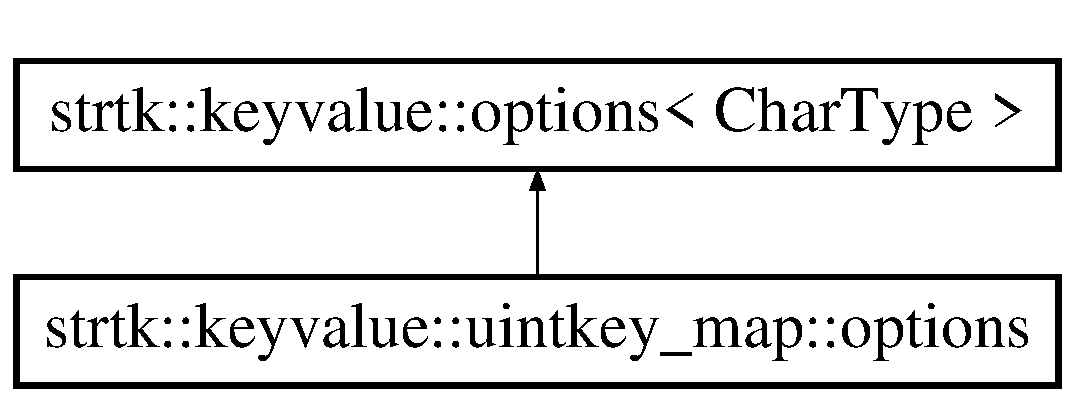
\includegraphics[height=2.000000cm]{structstrtk_1_1keyvalue_1_1options}
\end{center}
\end{figure}
\subsection*{Public Types}
\begin{DoxyCompactItemize}
\item 
\hypertarget{structstrtk_1_1keyvalue_1_1options_ad4361678bdc8f766b70451854ec3ba0d}{typedef Char\-Type {\bfseries char\-\_\-type}}\label{structstrtk_1_1keyvalue_1_1options_ad4361678bdc8f766b70451854ec3ba0d}

\end{DoxyCompactItemize}
\subsection*{Public Attributes}
\begin{DoxyCompactItemize}
\item 
\hypertarget{structstrtk_1_1keyvalue_1_1options_ae15030598c80b0bd6f4379107f808990}{char\-\_\-type {\bfseries pair\-\_\-block\-\_\-delimiter}}\label{structstrtk_1_1keyvalue_1_1options_ae15030598c80b0bd6f4379107f808990}

\item 
\hypertarget{structstrtk_1_1keyvalue_1_1options_aa6383930234c4a010de684299528ca4f}{char\-\_\-type {\bfseries pair\-\_\-delimiter}}\label{structstrtk_1_1keyvalue_1_1options_aa6383930234c4a010de684299528ca4f}

\end{DoxyCompactItemize}


The documentation for this struct was generated from the following file\-:\begin{DoxyCompactItemize}
\item 
strtk.\-hpp\end{DoxyCompactItemize}

\hypertarget{structstrtk_1_1keyvalue_1_1uintkey__map_1_1options}{\section{strtk\-:\-:keyvalue\-:\-:uintkey\-\_\-map\-:\-:options Struct Reference}
\label{structstrtk_1_1keyvalue_1_1uintkey__map_1_1options}\index{strtk\-::keyvalue\-::uintkey\-\_\-map\-::options@{strtk\-::keyvalue\-::uintkey\-\_\-map\-::options}}
}
Inheritance diagram for strtk\-:\-:keyvalue\-:\-:uintkey\-\_\-map\-:\-:options\-:\begin{figure}[H]
\begin{center}
\leavevmode
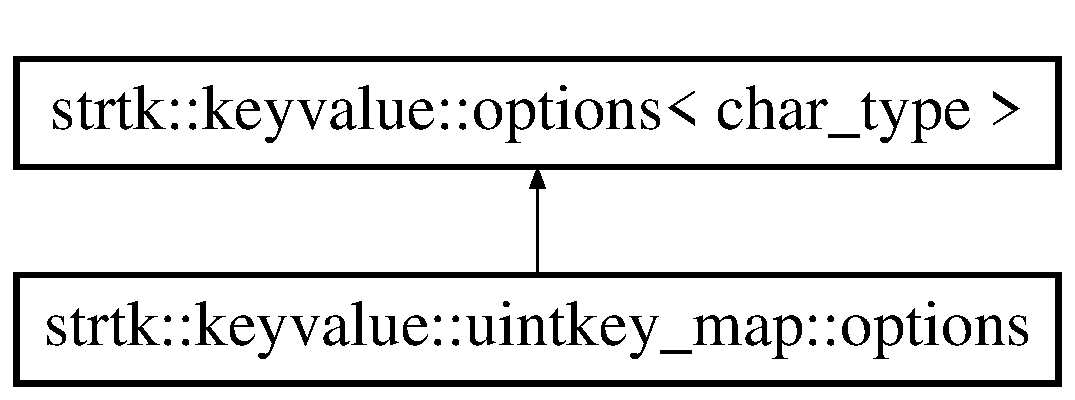
\includegraphics[height=2.000000cm]{structstrtk_1_1keyvalue_1_1uintkey__map_1_1options}
\end{center}
\end{figure}
\subsection*{Public Attributes}
\begin{DoxyCompactItemize}
\item 
\hypertarget{structstrtk_1_1keyvalue_1_1uintkey__map_1_1options_a6fb95ce517e172538b187ffd5b410f60}{std\-::size\-\_\-t {\bfseries key\-\_\-count}}\label{structstrtk_1_1keyvalue_1_1uintkey__map_1_1options_a6fb95ce517e172538b187ffd5b410f60}

\end{DoxyCompactItemize}
\subsection*{Additional Inherited Members}


The documentation for this struct was generated from the following file\-:\begin{DoxyCompactItemize}
\item 
strtk.\-hpp\end{DoxyCompactItemize}

\hypertarget{structstrtk_1_1token__grid_1_1options}{\section{strtk\-:\-:token\-\_\-grid\-:\-:options Struct Reference}
\label{structstrtk_1_1token__grid_1_1options}\index{strtk\-::token\-\_\-grid\-::options@{strtk\-::token\-\_\-grid\-::options}}
}
\subsection*{Public Member Functions}
\begin{DoxyCompactItemize}
\item 
\hypertarget{structstrtk_1_1token__grid_1_1options_a44c176a8122b9a3e24846ea909488ff0}{{\bfseries options} (split\-\_\-options\-::type sro, split\-\_\-options\-::type sco, const std\-::string \&rd, const std\-::string \&cd, const bool support\-\_\-dq=false, const bool trim\-\_\-dq=false)}\label{structstrtk_1_1token__grid_1_1options_a44c176a8122b9a3e24846ea909488ff0}

\item 
\hypertarget{structstrtk_1_1token__grid_1_1options_a8f4e80af24af3a27c148f3b27ba459d7}{\hyperlink{structstrtk_1_1token__grid_1_1options}{options} \& {\bfseries set\-\_\-column\-\_\-split\-\_\-option} (const split\-\_\-options\-::type \&option)}\label{structstrtk_1_1token__grid_1_1options_a8f4e80af24af3a27c148f3b27ba459d7}

\item 
\hypertarget{structstrtk_1_1token__grid_1_1options_ab14faa5018e837b307adde7409684402}{\hyperlink{structstrtk_1_1token__grid_1_1options}{options} \& {\bfseries set\-\_\-row\-\_\-split\-\_\-option} (const split\-\_\-options\-::type \&option)}\label{structstrtk_1_1token__grid_1_1options_ab14faa5018e837b307adde7409684402}

\item 
\hypertarget{structstrtk_1_1token__grid_1_1options_a0626480209944c0a104bd8f000af35b3}{\hyperlink{structstrtk_1_1token__grid_1_1options}{options} \& {\bfseries set\-\_\-column\-\_\-delimiters} (const std\-::string \&delimiters)}\label{structstrtk_1_1token__grid_1_1options_a0626480209944c0a104bd8f000af35b3}

\item 
\hypertarget{structstrtk_1_1token__grid_1_1options_a01057a1f67833b3c2ec9b435e160107b}{\hyperlink{structstrtk_1_1token__grid_1_1options}{options} \& {\bfseries set\-\_\-row\-\_\-delimiters} (const std\-::string \&delimiters)}\label{structstrtk_1_1token__grid_1_1options_a01057a1f67833b3c2ec9b435e160107b}

\end{DoxyCompactItemize}
\subsection*{Public Attributes}
\begin{DoxyCompactItemize}
\item 
\hypertarget{structstrtk_1_1token__grid_1_1options_a37711a26d2bd83d04107cf87e8893cf1}{split\-\_\-options\-::type {\bfseries row\-\_\-split\-\_\-option}}\label{structstrtk_1_1token__grid_1_1options_a37711a26d2bd83d04107cf87e8893cf1}

\item 
\hypertarget{structstrtk_1_1token__grid_1_1options_aa191493315b3802d1ee3b12c8bd0553e}{split\-\_\-options\-::type {\bfseries column\-\_\-split\-\_\-option}}\label{structstrtk_1_1token__grid_1_1options_aa191493315b3802d1ee3b12c8bd0553e}

\item 
\hypertarget{structstrtk_1_1token__grid_1_1options_abd58aa3a83066f92ef50a52055e42bc6}{std\-::string {\bfseries row\-\_\-delimiters}}\label{structstrtk_1_1token__grid_1_1options_abd58aa3a83066f92ef50a52055e42bc6}

\item 
\hypertarget{structstrtk_1_1token__grid_1_1options_a822c2ffc81765ec5b7e2091b64f88a5f}{std\-::string {\bfseries column\-\_\-delimiters}}\label{structstrtk_1_1token__grid_1_1options_a822c2ffc81765ec5b7e2091b64f88a5f}

\item 
\hypertarget{structstrtk_1_1token__grid_1_1options_a6f21807635d2077fab1cb2dd5f8c267c}{bool {\bfseries support\-\_\-dquotes}}\label{structstrtk_1_1token__grid_1_1options_a6f21807635d2077fab1cb2dd5f8c267c}

\item 
\hypertarget{structstrtk_1_1token__grid_1_1options_a2aeb182400c23da8783790a175471f81}{bool {\bfseries trim\-\_\-dquotes}}\label{structstrtk_1_1token__grid_1_1options_a2aeb182400c23da8783790a175471f81}

\end{DoxyCompactItemize}


The documentation for this struct was generated from the following file\-:\begin{DoxyCompactItemize}
\item 
strtk.\-hpp\end{DoxyCompactItemize}

\hypertarget{classstrtk_1_1bloom_1_1parameters}{\section{strtk\-:\-:bloom\-:\-:parameters Class Reference}
\label{classstrtk_1_1bloom_1_1parameters}\index{strtk\-::bloom\-::parameters@{strtk\-::bloom\-::parameters}}
}
\subsection*{Classes}
\begin{DoxyCompactItemize}
\item 
struct \hyperlink{structstrtk_1_1bloom_1_1parameters_1_1optimal__parameters__t}{optimal\-\_\-parameters\-\_\-t}
\end{DoxyCompactItemize}
\subsection*{Public Member Functions}
\begin{DoxyCompactItemize}
\item 
\hypertarget{classstrtk_1_1bloom_1_1parameters_a7a5017ee4ee5c59d18a8c2dabb10251b}{bool {\bfseries operator!} ()}\label{classstrtk_1_1bloom_1_1parameters_a7a5017ee4ee5c59d18a8c2dabb10251b}

\item 
\hypertarget{classstrtk_1_1bloom_1_1parameters_a96af110ad78a5732aac03001c4317a72}{bool {\bfseries operator()} (\hyperlink{classstrtk_1_1binary_1_1reader}{strtk\-::binary\-::reader} \&reader)}\label{classstrtk_1_1bloom_1_1parameters_a96af110ad78a5732aac03001c4317a72}

\item 
\hypertarget{classstrtk_1_1bloom_1_1parameters_a5b46dd32cd01e0528acfdb445fa3589d}{bool {\bfseries operator()} (\hyperlink{classstrtk_1_1binary_1_1writer}{strtk\-::binary\-::writer} \&writer)}\label{classstrtk_1_1bloom_1_1parameters_a5b46dd32cd01e0528acfdb445fa3589d}

\item 
\hypertarget{classstrtk_1_1bloom_1_1parameters_a5f4e0228dc0cc6e7c43364e1c48d9bb8}{virtual bool {\bfseries compute\-\_\-optimal\-\_\-parameters} ()}\label{classstrtk_1_1bloom_1_1parameters_a5f4e0228dc0cc6e7c43364e1c48d9bb8}

\end{DoxyCompactItemize}
\subsection*{Public Attributes}
\begin{DoxyCompactItemize}
\item 
\hypertarget{classstrtk_1_1bloom_1_1parameters_a262807e5a6860957ce855e66f42d4dac}{unsigned long long int {\bfseries minimum\-\_\-size}}\label{classstrtk_1_1bloom_1_1parameters_a262807e5a6860957ce855e66f42d4dac}

\item 
\hypertarget{classstrtk_1_1bloom_1_1parameters_a2a38ac9675e0d143172ed79acc388a08}{unsigned long long int {\bfseries maximum\-\_\-size}}\label{classstrtk_1_1bloom_1_1parameters_a2a38ac9675e0d143172ed79acc388a08}

\item 
\hypertarget{classstrtk_1_1bloom_1_1parameters_a55b2f070fbb00c248ddeede1ce17aec7}{unsigned int {\bfseries minimum\-\_\-number\-\_\-of\-\_\-hashes}}\label{classstrtk_1_1bloom_1_1parameters_a55b2f070fbb00c248ddeede1ce17aec7}

\item 
\hypertarget{classstrtk_1_1bloom_1_1parameters_a1da499c323f86823378a47364f4edaf7}{unsigned int {\bfseries maximum\-\_\-number\-\_\-of\-\_\-hashes}}\label{classstrtk_1_1bloom_1_1parameters_a1da499c323f86823378a47364f4edaf7}

\item 
\hypertarget{classstrtk_1_1bloom_1_1parameters_ab64de09806e1f2655dad875e75aeef5f}{unsigned long long int {\bfseries projected\-\_\-element\-\_\-count}}\label{classstrtk_1_1bloom_1_1parameters_ab64de09806e1f2655dad875e75aeef5f}

\item 
\hypertarget{classstrtk_1_1bloom_1_1parameters_a86679bd51d774f9d52b60098c4922120}{double {\bfseries false\-\_\-positive\-\_\-probability}}\label{classstrtk_1_1bloom_1_1parameters_a86679bd51d774f9d52b60098c4922120}

\item 
\hypertarget{classstrtk_1_1bloom_1_1parameters_a1230bb767861b076c57042f17f94631c}{unsigned long long int {\bfseries random\-\_\-seed}}\label{classstrtk_1_1bloom_1_1parameters_a1230bb767861b076c57042f17f94631c}

\item 
\hypertarget{classstrtk_1_1bloom_1_1parameters_a6362ce41a912c689a3a5af08666000c8}{\hyperlink{structstrtk_1_1bloom_1_1parameters_1_1optimal__parameters__t}{optimal\-\_\-parameters\-\_\-t} {\bfseries optimal\-\_\-parameters}}\label{classstrtk_1_1bloom_1_1parameters_a6362ce41a912c689a3a5af08666000c8}

\end{DoxyCompactItemize}


The documentation for this class was generated from the following file\-:\begin{DoxyCompactItemize}
\item 
strtk.\-hpp\end{DoxyCompactItemize}

\hypertarget{classrapidxml_1_1parse__error}{\section{rapidxml\-:\-:parse\-\_\-error Class Reference}
\label{classrapidxml_1_1parse__error}\index{rapidxml\-::parse\-\_\-error@{rapidxml\-::parse\-\_\-error}}
}


{\ttfamily \#include $<$rapidxml.\-hpp$>$}

Inheritance diagram for rapidxml\-:\-:parse\-\_\-error\-:\begin{figure}[H]
\begin{center}
\leavevmode
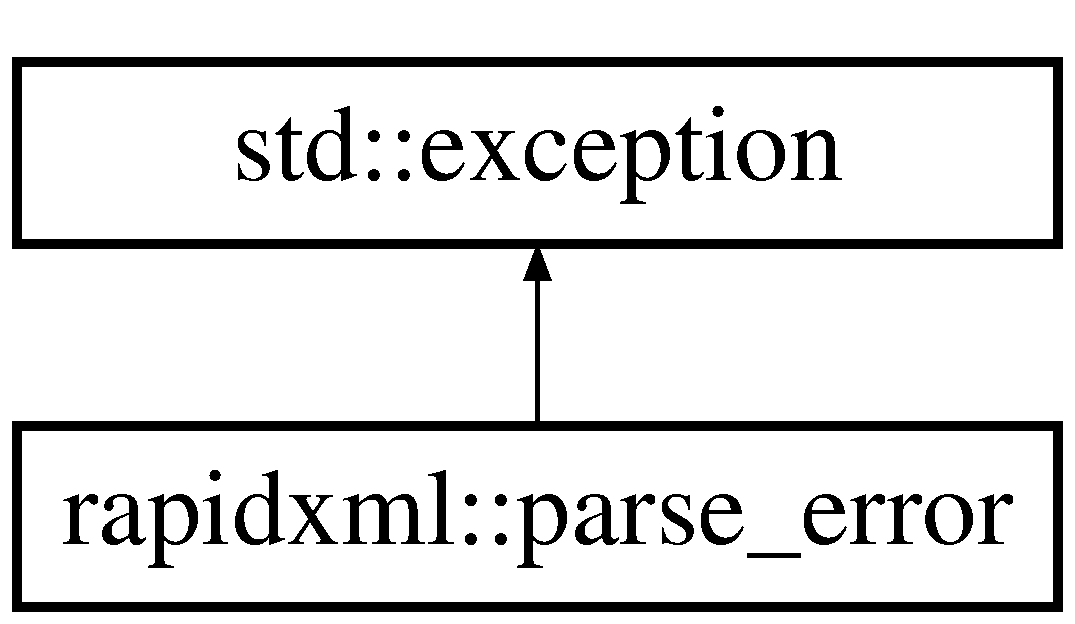
\includegraphics[height=2.000000cm]{classrapidxml_1_1parse__error}
\end{center}
\end{figure}
\subsection*{Public Member Functions}
\begin{DoxyCompactItemize}
\item 
\hypertarget{classrapidxml_1_1parse__error_aea12a301271c393fb627b368fb9f35c1}{\hyperlink{classrapidxml_1_1parse__error_aea12a301271c393fb627b368fb9f35c1}{parse\-\_\-error} (const char $\ast$\hyperlink{classrapidxml_1_1parse__error_a7665c88639e7466ee1de388a4f85e6fe}{what}, void $\ast$\hyperlink{classrapidxml_1_1parse__error_a3a0ab9e586c1d2b437c340f6622fbec6}{where})}\label{classrapidxml_1_1parse__error_aea12a301271c393fb627b368fb9f35c1}

\begin{DoxyCompactList}\small\item\em Constructs parse error. \end{DoxyCompactList}\item 
virtual const char $\ast$ \hyperlink{classrapidxml_1_1parse__error_a7665c88639e7466ee1de388a4f85e6fe}{what} () const   throw ()
\item 
{\footnotesize template$<$class Ch $>$ }\\Ch $\ast$ \hyperlink{classrapidxml_1_1parse__error_a3a0ab9e586c1d2b437c340f6622fbec6}{where} () const 
\end{DoxyCompactItemize}


\subsection{Detailed Description}
Parse error exception. This exception is thrown by the parser when an error occurs. Use \hyperlink{classrapidxml_1_1parse__error_a7665c88639e7466ee1de388a4f85e6fe}{what()} function to get human-\/readable error message. Use \hyperlink{classrapidxml_1_1parse__error_a3a0ab9e586c1d2b437c340f6622fbec6}{where()} function to get a pointer to position within source text where error was detected. \par
\par
 If throwing exceptions by the parser is undesirable, it can be disabled by defining R\-A\-P\-I\-D\-X\-M\-L\-\_\-\-N\-O\-\_\-\-E\-X\-C\-E\-P\-T\-I\-O\-N\-S macro before \hyperlink{rapidxml_8hpp}{rapidxml.\-hpp} is included. This will cause the parser to call rapidxml\-::parse\-\_\-error\-\_\-handler() function instead of throwing an exception. This function must be defined by the user. \par
\par
 This class derives from {\ttfamily std\-::exception} class. 

\subsection{Member Function Documentation}
\hypertarget{classrapidxml_1_1parse__error_a7665c88639e7466ee1de388a4f85e6fe}{\index{rapidxml\-::parse\-\_\-error@{rapidxml\-::parse\-\_\-error}!what@{what}}
\index{what@{what}!rapidxml::parse_error@{rapidxml\-::parse\-\_\-error}}
\subsubsection[{what}]{\setlength{\rightskip}{0pt plus 5cm}virtual const char$\ast$ rapidxml\-::parse\-\_\-error\-::what (
\begin{DoxyParamCaption}
{}
\end{DoxyParamCaption}
) const throw  ) \hspace{0.3cm}{\ttfamily [inline]}, {\ttfamily [virtual]}}}\label{classrapidxml_1_1parse__error_a7665c88639e7466ee1de388a4f85e6fe}
Gets human readable description of error. \begin{DoxyReturn}{Returns}
Pointer to null terminated description of the error. 
\end{DoxyReturn}
\hypertarget{classrapidxml_1_1parse__error_a3a0ab9e586c1d2b437c340f6622fbec6}{\index{rapidxml\-::parse\-\_\-error@{rapidxml\-::parse\-\_\-error}!where@{where}}
\index{where@{where}!rapidxml::parse_error@{rapidxml\-::parse\-\_\-error}}
\subsubsection[{where}]{\setlength{\rightskip}{0pt plus 5cm}template$<$class Ch $>$ Ch$\ast$ rapidxml\-::parse\-\_\-error\-::where (
\begin{DoxyParamCaption}
{}
\end{DoxyParamCaption}
) const\hspace{0.3cm}{\ttfamily [inline]}}}\label{classrapidxml_1_1parse__error_a3a0ab9e586c1d2b437c340f6622fbec6}
Gets pointer to character data where error happened. Ch should be the same as char type of \hyperlink{classrapidxml_1_1xml__document}{xml\-\_\-document} that produced the error. \begin{DoxyReturn}{Returns}
Pointer to location within the parsed string where error occured. 
\end{DoxyReturn}


The documentation for this class was generated from the following file\-:\begin{DoxyCompactItemize}
\item 
\hyperlink{rapidxml_8hpp}{rapidxml.\-hpp}\end{DoxyCompactItemize}

\hypertarget{classParser}{\section{Parser Class Reference}
\label{classParser}\index{Parser@{Parser}}
}
\subsection*{Public Member Functions}
\begin{DoxyCompactItemize}
\item 
\hypertarget{classParser_ac910dcda772ee8ed3c271cd7f8bfd21e}{{\bfseries Parser} (\hyperlink{classDictionary}{Dictionary} $\ast$\&)}\label{classParser_ac910dcda772ee8ed3c271cd7f8bfd21e}

\end{DoxyCompactItemize}


The documentation for this class was generated from the following files\-:\begin{DoxyCompactItemize}
\item 
Parser.\-h\item 
Parser.\-cpp\end{DoxyCompactItemize}

\hypertarget{classstrtk_1_1keyvalue_1_1parser}{\section{strtk\-:\-:keyvalue\-:\-:parser$<$ Key\-Value\-Map $>$ Class Template Reference}
\label{classstrtk_1_1keyvalue_1_1parser}\index{strtk\-::keyvalue\-::parser$<$ Key\-Value\-Map $>$@{strtk\-::keyvalue\-::parser$<$ Key\-Value\-Map $>$}}
}
\subsection*{Public Types}
\begin{DoxyCompactItemize}
\item 
\hypertarget{classstrtk_1_1keyvalue_1_1parser_abd76c940f5a4fefe824da214508f3401}{typedef unsigned char {\bfseries char\-\_\-type}}\label{classstrtk_1_1keyvalue_1_1parser_abd76c940f5a4fefe824da214508f3401}

\item 
\hypertarget{classstrtk_1_1keyvalue_1_1parser_a9a40a018d668c4c49248a74f2161a559}{typedef std\-::pair$<$ char\-\_\-type \\*
$\ast$, char\-\_\-type $\ast$ $>$ {\bfseries range\-\_\-type}}\label{classstrtk_1_1keyvalue_1_1parser_a9a40a018d668c4c49248a74f2161a559}

\end{DoxyCompactItemize}
\subsection*{Public Member Functions}
\begin{DoxyCompactItemize}
\item 
\hypertarget{classstrtk_1_1keyvalue_1_1parser_acea2a28b0fb6ac984d3c3c27a32b3b65}{{\footnotesize template$<$typename Options $>$ }\\{\bfseries parser} (const Options \&opts)}\label{classstrtk_1_1keyvalue_1_1parser_acea2a28b0fb6ac984d3c3c27a32b3b65}

\item 
\hypertarget{classstrtk_1_1keyvalue_1_1parser_a14eb155de12e3fc6cc9980ca8a73740e}{{\footnotesize template$<$typename T $>$ }\\bool {\bfseries register\-\_\-keyvalue} (const typename Key\-Value\-Map\-::key\-\_\-type \&key, T \&t)}\label{classstrtk_1_1keyvalue_1_1parser_a14eb155de12e3fc6cc9980ca8a73740e}

\item 
\hypertarget{classstrtk_1_1keyvalue_1_1parser_a3c200d4cccbb36f2ea0ae470bbb6c618}{bool {\bfseries operator()} (const range\-\_\-type \&data, const bool ignore\-\_\-failures=false)}\label{classstrtk_1_1keyvalue_1_1parser_a3c200d4cccbb36f2ea0ae470bbb6c618}

\item 
\hypertarget{classstrtk_1_1keyvalue_1_1parser_a02698da1a1fa442afbab2b423bdaad57}{bool {\bfseries operator()} (const std\-::string \&s, const bool ignore\-\_\-failures=false)}\label{classstrtk_1_1keyvalue_1_1parser_a02698da1a1fa442afbab2b423bdaad57}

\item 
\hypertarget{classstrtk_1_1keyvalue_1_1parser_a7ab652f64d5adb204083f4b31ec82805}{std\-::size\-\_\-t {\bfseries failure\-\_\-count} () const }\label{classstrtk_1_1keyvalue_1_1parser_a7ab652f64d5adb204083f4b31ec82805}

\end{DoxyCompactItemize}


The documentation for this class was generated from the following file\-:\begin{DoxyCompactItemize}
\item 
strtk.\-hpp\end{DoxyCompactItemize}

\hypertarget{classstrtk_1_1trie_1_1prefix}{\section{strtk\-:\-:trie\-:\-:prefix$<$ Key\-Iterator, Value\-Type $>$ Class Template Reference}
\label{classstrtk_1_1trie_1_1prefix}\index{strtk\-::trie\-::prefix$<$ Key\-Iterator, Value\-Type $>$@{strtk\-::trie\-::prefix$<$ Key\-Iterator, Value\-Type $>$}}
}
\subsection*{Public Types}
\begin{DoxyCompactItemize}
\item 
\hypertarget{classstrtk_1_1trie_1_1prefix_a23ef899d485148d2cee823d51730c4a6}{typedef std\-::iterator\-\_\-traits\\*
$<$ Key\-Iterator $>$\-::value\-\_\-type {\bfseries key\-\_\-value\-\_\-t}}\label{classstrtk_1_1trie_1_1prefix_a23ef899d485148d2cee823d51730c4a6}

\item 
\hypertarget{classstrtk_1_1trie_1_1prefix_a3b878f89a888e4ef4f853c20101155b9}{typedef Value\-Type {\bfseries value\-\_\-t}}\label{classstrtk_1_1trie_1_1prefix_a3b878f89a888e4ef4f853c20101155b9}

\item 
\hypertarget{classstrtk_1_1trie_1_1prefix_a240ea8030c5db8e1a843623a6860dd73}{typedef node$<$ Key\-Iterator, \\*
value\-\_\-t $>$ {\bfseries node\-\_\-t}}\label{classstrtk_1_1trie_1_1prefix_a240ea8030c5db8e1a843623a6860dd73}

\item 
\hypertarget{classstrtk_1_1trie_1_1prefix_a3bdf863ed8141cd866ddebc3b20c142d}{typedef node\-\_\-t $\ast$ {\bfseries node\-\_\-ptr}}\label{classstrtk_1_1trie_1_1prefix_a3bdf863ed8141cd866ddebc3b20c142d}

\end{DoxyCompactItemize}
\subsection*{Public Member Functions}
\begin{DoxyCompactItemize}
\item 
\hypertarget{classstrtk_1_1trie_1_1prefix_a14ec25433dff5812a0a7f5856697c15c}{{\footnotesize template$<$typename key\-\_\-iterator\-\_\-t $>$ }\\void {\bfseries insert} (const key\-\_\-iterator\-\_\-t begin, const key\-\_\-iterator\-\_\-t end, const value\-\_\-t \&v)}\label{classstrtk_1_1trie_1_1prefix_a14ec25433dff5812a0a7f5856697c15c}

\item 
\hypertarget{classstrtk_1_1trie_1_1prefix_a2bef2459f617c0b59515cd74525019e8}{{\footnotesize template$<$typename key\-\_\-iterator\-\_\-t $>$ }\\bool {\bfseries find} (const key\-\_\-iterator\-\_\-t begin, const key\-\_\-iterator\-\_\-t end, value\-\_\-t \&v) const }\label{classstrtk_1_1trie_1_1prefix_a2bef2459f617c0b59515cd74525019e8}

\item 
\hypertarget{classstrtk_1_1trie_1_1prefix_ae3c282734d52ea54198d4a38a07926fa}{{\footnotesize template$<$typename key\-\_\-iterator\-\_\-t $>$ }\\bool {\bfseries find\-\_\-prefix} (const key\-\_\-iterator\-\_\-t begin, const key\-\_\-iterator\-\_\-t end) const }\label{classstrtk_1_1trie_1_1prefix_ae3c282734d52ea54198d4a38a07926fa}

\end{DoxyCompactItemize}


The documentation for this class was generated from the following file\-:\begin{DoxyCompactItemize}
\item 
strtk.\-hpp\end{DoxyCompactItemize}

\hypertarget{structstrtk_1_1prefix__trie}{\section{strtk\-:\-:prefix\-\_\-trie$<$ Value\-Type, Key\-Iterator $>$ Struct Template Reference}
\label{structstrtk_1_1prefix__trie}\index{strtk\-::prefix\-\_\-trie$<$ Value\-Type, Key\-Iterator $>$@{strtk\-::prefix\-\_\-trie$<$ Value\-Type, Key\-Iterator $>$}}
}
\subsection*{Public Types}
\begin{DoxyCompactItemize}
\item 
\hypertarget{structstrtk_1_1prefix__trie_a3b8576c6c1e6c258ad45da3ddec60171}{typedef \hyperlink{classstrtk_1_1trie_1_1prefix}{trie\-::prefix}\\*
$<$ Key\-Iterator, Value\-Type $>$ {\bfseries type}}\label{structstrtk_1_1prefix__trie_a3b8576c6c1e6c258ad45da3ddec60171}

\item 
\hypertarget{structstrtk_1_1prefix__trie_aed3fc66a7fe65ffa4c0fe4c40e800bf0}{typedef \hyperlink{classstrtk_1_1trie_1_1prefix}{trie\-::prefix}\\*
$<$ Key\-Iterator, Value\-Type $>$ {\bfseries std\-\_\-string}}\label{structstrtk_1_1prefix__trie_aed3fc66a7fe65ffa4c0fe4c40e800bf0}

\item 
\hypertarget{structstrtk_1_1prefix__trie_a1a33be4fe30aa3fcf46d4d48724c8a82}{typedef \hyperlink{classstrtk_1_1trie_1_1prefix}{trie\-::prefix}$<$ char \\*
$\ast$, Value\-Type $>$ {\bfseries char\-\_\-ptr}}\label{structstrtk_1_1prefix__trie_a1a33be4fe30aa3fcf46d4d48724c8a82}

\item 
\hypertarget{structstrtk_1_1prefix__trie_ae65e4c315ef9582c41f3f7269d7defee}{typedef \hyperlink{classstrtk_1_1trie_1_1prefix}{trie\-::prefix}$<$ const \\*
char $\ast$, Value\-Type $>$ {\bfseries const\-\_\-char\-\_\-ptr}}\label{structstrtk_1_1prefix__trie_ae65e4c315ef9582c41f3f7269d7defee}

\item 
\hypertarget{structstrtk_1_1prefix__trie_a1169ae7eceefc8220dea284354d82bc7}{typedef \hyperlink{classstrtk_1_1trie_1_1prefix}{trie\-::prefix}$<$ unsigned \\*
char $\ast$, Value\-Type $>$ {\bfseries uchar\-\_\-ptr}}\label{structstrtk_1_1prefix__trie_a1169ae7eceefc8220dea284354d82bc7}

\item 
\hypertarget{structstrtk_1_1prefix__trie_a29816064f1519e463a38ee81c1d037fc}{typedef \hyperlink{classstrtk_1_1trie_1_1prefix}{trie\-::prefix}$<$ const \\*
unsigned char $\ast$, Value\-Type $>$ {\bfseries const\-\_\-uchar\-\_\-ptr}}\label{structstrtk_1_1prefix__trie_a29816064f1519e463a38ee81c1d037fc}

\end{DoxyCompactItemize}


The documentation for this struct was generated from the following file\-:\begin{DoxyCompactItemize}
\item 
strtk.\-hpp\end{DoxyCompactItemize}

\hypertarget{structstrtk_1_1priority__queue__sink}{\section{strtk\-:\-:priority\-\_\-queue\-\_\-sink$<$ T $>$ Struct Template Reference}
\label{structstrtk_1_1priority__queue__sink}\index{strtk\-::priority\-\_\-queue\-\_\-sink$<$ T $>$@{strtk\-::priority\-\_\-queue\-\_\-sink$<$ T $>$}}
}
\subsection*{Public Types}
\begin{DoxyCompactItemize}
\item 
\hypertarget{structstrtk_1_1priority__queue__sink_ade0288bfe1ac5e629da5fca2a370fc1b}{typedef \hyperlink{classstrtk_1_1sink__type}{sink\-\_\-type}\\*
$<$ std\-::priority\-\_\-queue$<$ T $>$ $>$ {\bfseries type}}\label{structstrtk_1_1priority__queue__sink_ade0288bfe1ac5e629da5fca2a370fc1b}

\end{DoxyCompactItemize}


The documentation for this struct was generated from the following file\-:\begin{DoxyCompactItemize}
\item 
strtk.\-hpp\end{DoxyCompactItemize}

\hypertarget{classstrtk_1_1push__inserter__iterator}{\section{strtk\-:\-:push\-\_\-inserter\-\_\-iterator$<$ Container $>$ Class Template Reference}
\label{classstrtk_1_1push__inserter__iterator}\index{strtk\-::push\-\_\-inserter\-\_\-iterator$<$ Container $>$@{strtk\-::push\-\_\-inserter\-\_\-iterator$<$ Container $>$}}
}
Inheritance diagram for strtk\-:\-:push\-\_\-inserter\-\_\-iterator$<$ Container $>$\-:\begin{figure}[H]
\begin{center}
\leavevmode
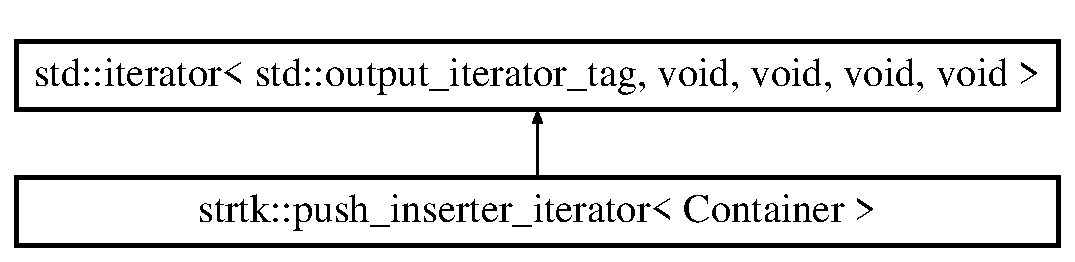
\includegraphics[height=2.000000cm]{classstrtk_1_1push__inserter__iterator}
\end{center}
\end{figure}
\subsection*{Public Member Functions}
\begin{DoxyCompactItemize}
\item 
\hypertarget{classstrtk_1_1push__inserter__iterator_a578f5c7cb54edbbb84c1d8d36b490c94}{{\bfseries push\-\_\-inserter\-\_\-iterator} (Container \&container)}\label{classstrtk_1_1push__inserter__iterator_a578f5c7cb54edbbb84c1d8d36b490c94}

\item 
\hypertarget{classstrtk_1_1push__inserter__iterator_ad251d0a2f0e580aa3d19f5334fba9a85}{\hyperlink{classstrtk_1_1push__inserter__iterator}{push\-\_\-inserter\-\_\-iterator} \& {\bfseries operator=} (const \hyperlink{classstrtk_1_1push__inserter__iterator}{push\-\_\-inserter\-\_\-iterator} \&itr)}\label{classstrtk_1_1push__inserter__iterator_ad251d0a2f0e580aa3d19f5334fba9a85}

\item 
\hypertarget{classstrtk_1_1push__inserter__iterator_aaa01d8f8bbe3f31ff9458000474964ae}{\hyperlink{classstrtk_1_1push__inserter__iterator}{push\-\_\-inserter\-\_\-iterator}\\*
$<$ Container $>$ \& {\bfseries operator=} (typename Container\-::const\-\_\-reference v)}\label{classstrtk_1_1push__inserter__iterator_aaa01d8f8bbe3f31ff9458000474964ae}

\item 
\hypertarget{classstrtk_1_1push__inserter__iterator_a44ef1eb80f538f200bdb865a9ff40c32}{\hyperlink{classstrtk_1_1push__inserter__iterator}{push\-\_\-inserter\-\_\-iterator}\\*
$<$ Container $>$ \& {\bfseries operator$\ast$} ()}\label{classstrtk_1_1push__inserter__iterator_a44ef1eb80f538f200bdb865a9ff40c32}

\item 
\hypertarget{classstrtk_1_1push__inserter__iterator_a1487f29071a3e248e9ee59b47d2e7b65}{\hyperlink{classstrtk_1_1push__inserter__iterator}{push\-\_\-inserter\-\_\-iterator}\\*
$<$ Container $>$ \& {\bfseries operator++} ()}\label{classstrtk_1_1push__inserter__iterator_a1487f29071a3e248e9ee59b47d2e7b65}

\item 
\hypertarget{classstrtk_1_1push__inserter__iterator_a03846ef51510282effffe5c55b213a4d}{\hyperlink{classstrtk_1_1push__inserter__iterator}{push\-\_\-inserter\-\_\-iterator}$<$ Container $>$ {\bfseries operator++} (int)}\label{classstrtk_1_1push__inserter__iterator_a03846ef51510282effffe5c55b213a4d}

\end{DoxyCompactItemize}


The documentation for this class was generated from the following file\-:\begin{DoxyCompactItemize}
\item 
strtk.\-hpp\end{DoxyCompactItemize}

\hypertarget{structstrtk_1_1queue__sink}{\section{strtk\-:\-:queue\-\_\-sink$<$ T $>$ Struct Template Reference}
\label{structstrtk_1_1queue__sink}\index{strtk\-::queue\-\_\-sink$<$ T $>$@{strtk\-::queue\-\_\-sink$<$ T $>$}}
}
\subsection*{Public Types}
\begin{DoxyCompactItemize}
\item 
\hypertarget{structstrtk_1_1queue__sink_ab1fdadb5ecf4cea9aa873354c81a565f}{typedef \hyperlink{classstrtk_1_1sink__type}{sink\-\_\-type}$<$ std\-::queue\\*
$<$ T $>$ $>$ {\bfseries type}}\label{structstrtk_1_1queue__sink_ab1fdadb5ecf4cea9aa873354c81a565f}

\end{DoxyCompactItemize}


The documentation for this struct was generated from the following file\-:\begin{DoxyCompactItemize}
\item 
strtk.\-hpp\end{DoxyCompactItemize}

\hypertarget{structstrtk_1_1details_1_1rand__int__type__tag}{\section{strtk\-:\-:details\-:\-:rand\-\_\-int\-\_\-type\-\_\-tag Struct Reference}
\label{structstrtk_1_1details_1_1rand__int__type__tag}\index{strtk\-::details\-::rand\-\_\-int\-\_\-type\-\_\-tag@{strtk\-::details\-::rand\-\_\-int\-\_\-type\-\_\-tag}}
}


The documentation for this struct was generated from the following file\-:\begin{DoxyCompactItemize}
\item 
strtk.\-hpp\end{DoxyCompactItemize}

\hypertarget{structstrtk_1_1details_1_1rand__real__type__tag}{\section{strtk\-:\-:details\-:\-:rand\-\_\-real\-\_\-type\-\_\-tag Struct Reference}
\label{structstrtk_1_1details_1_1rand__real__type__tag}\index{strtk\-::details\-::rand\-\_\-real\-\_\-type\-\_\-tag@{strtk\-::details\-::rand\-\_\-real\-\_\-type\-\_\-tag}}
}


The documentation for this struct was generated from the following file\-:\begin{DoxyCompactItemize}
\item 
strtk.\-hpp\end{DoxyCompactItemize}

\hypertarget{classstrtk_1_1range__to__ptr__type__iterator}{\section{strtk\-:\-:range\-\_\-to\-\_\-ptr\-\_\-type\-\_\-iterator$<$ T $>$ Class Template Reference}
\label{classstrtk_1_1range__to__ptr__type__iterator}\index{strtk\-::range\-\_\-to\-\_\-ptr\-\_\-type\-\_\-iterator$<$ T $>$@{strtk\-::range\-\_\-to\-\_\-ptr\-\_\-type\-\_\-iterator$<$ T $>$}}
}
Inheritance diagram for strtk\-:\-:range\-\_\-to\-\_\-ptr\-\_\-type\-\_\-iterator$<$ T $>$\-:\begin{figure}[H]
\begin{center}
\leavevmode
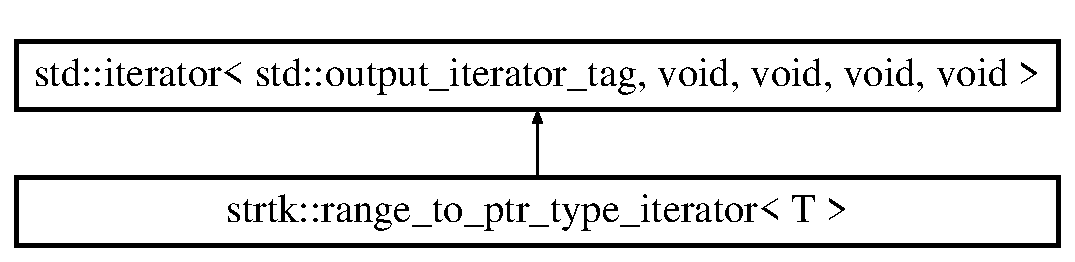
\includegraphics[height=2.000000cm]{classstrtk_1_1range__to__ptr__type__iterator}
\end{center}
\end{figure}
\subsection*{Public Types}
\begin{DoxyCompactItemize}
\item 
\hypertarget{classstrtk_1_1range__to__ptr__type__iterator_a466df1043c4eb962c01e5acf97285a23}{typedef T {\bfseries value\-\_\-type}}\label{classstrtk_1_1range__to__ptr__type__iterator_a466df1043c4eb962c01e5acf97285a23}

\end{DoxyCompactItemize}
\subsection*{Public Member Functions}
\begin{DoxyCompactItemize}
\item 
\hypertarget{classstrtk_1_1range__to__ptr__type__iterator_a46f717471fa10adb53b3da3490d43992}{{\bfseries range\-\_\-to\-\_\-ptr\-\_\-type\-\_\-iterator} (T $\ast$pointer, std\-::size\-\_\-t \&insert\-\_\-count)}\label{classstrtk_1_1range__to__ptr__type__iterator_a46f717471fa10adb53b3da3490d43992}

\item 
\hypertarget{classstrtk_1_1range__to__ptr__type__iterator_acac3919cea1a78cadb6c761ecc152e2c}{{\bfseries range\-\_\-to\-\_\-ptr\-\_\-type\-\_\-iterator} (const \hyperlink{classstrtk_1_1range__to__ptr__type__iterator}{range\-\_\-to\-\_\-ptr\-\_\-type\-\_\-iterator} \&itr)}\label{classstrtk_1_1range__to__ptr__type__iterator_acac3919cea1a78cadb6c761ecc152e2c}

\item 
\hypertarget{classstrtk_1_1range__to__ptr__type__iterator_a3ea71701ab3abe434dc8a79956b03e06}{\hyperlink{classstrtk_1_1range__to__ptr__type__iterator}{range\-\_\-to\-\_\-ptr\-\_\-type\-\_\-iterator} \& {\bfseries operator=} (const \hyperlink{classstrtk_1_1range__to__ptr__type__iterator}{range\-\_\-to\-\_\-ptr\-\_\-type\-\_\-iterator} \&itr)}\label{classstrtk_1_1range__to__ptr__type__iterator_a3ea71701ab3abe434dc8a79956b03e06}

\item 
\hypertarget{classstrtk_1_1range__to__ptr__type__iterator_ad0f04f4f9663ba5a0e49eef84a4f0122}{{\footnotesize template$<$typename Iterator $>$ }\\\hyperlink{classstrtk_1_1range__to__ptr__type__iterator}{range\-\_\-to\-\_\-ptr\-\_\-type\-\_\-iterator} \& {\bfseries operator=} (const std\-::pair$<$ Iterator, Iterator $>$ \&r)}\label{classstrtk_1_1range__to__ptr__type__iterator_ad0f04f4f9663ba5a0e49eef84a4f0122}

\item 
\hypertarget{classstrtk_1_1range__to__ptr__type__iterator_a1378342a0247b8398ccf4980b9afa189}{\hyperlink{classstrtk_1_1range__to__ptr__type__iterator}{range\-\_\-to\-\_\-ptr\-\_\-type\-\_\-iterator} \& {\bfseries operator=} (const std\-::string \&s)}\label{classstrtk_1_1range__to__ptr__type__iterator_a1378342a0247b8398ccf4980b9afa189}

\item 
\hypertarget{classstrtk_1_1range__to__ptr__type__iterator_a9a835ce6a8113b2b5d45c29af8c4a136}{{\footnotesize template$<$typename Iterator $>$ }\\void {\bfseries operator()} (const std\-::pair$<$ Iterator, Iterator $>$ \&r) const }\label{classstrtk_1_1range__to__ptr__type__iterator_a9a835ce6a8113b2b5d45c29af8c4a136}

\item 
\hypertarget{classstrtk_1_1range__to__ptr__type__iterator_aef33d1f18d62fd382ede6c9c7f725cda}{{\footnotesize template$<$typename Iterator $>$ }\\void {\bfseries operator()} (const Iterator begin, const Iterator end)}\label{classstrtk_1_1range__to__ptr__type__iterator_aef33d1f18d62fd382ede6c9c7f725cda}

\item 
\hypertarget{classstrtk_1_1range__to__ptr__type__iterator_a9a209d4ca0002d50b1e841dfe73a6cce}{\hyperlink{classstrtk_1_1range__to__ptr__type__iterator}{range\-\_\-to\-\_\-ptr\-\_\-type\-\_\-iterator} \& {\bfseries operator$\ast$} ()}\label{classstrtk_1_1range__to__ptr__type__iterator_a9a209d4ca0002d50b1e841dfe73a6cce}

\item 
\hypertarget{classstrtk_1_1range__to__ptr__type__iterator_a1be3dc2e4f582d418835074f7fd76a6e}{\hyperlink{classstrtk_1_1range__to__ptr__type__iterator}{range\-\_\-to\-\_\-ptr\-\_\-type\-\_\-iterator} \& {\bfseries operator++} ()}\label{classstrtk_1_1range__to__ptr__type__iterator_a1be3dc2e4f582d418835074f7fd76a6e}

\item 
\hypertarget{classstrtk_1_1range__to__ptr__type__iterator_a74659e255fefa0d49e36535ba2dc2acd}{\hyperlink{classstrtk_1_1range__to__ptr__type__iterator}{range\-\_\-to\-\_\-ptr\-\_\-type\-\_\-iterator} {\bfseries operator++} (int)}\label{classstrtk_1_1range__to__ptr__type__iterator_a74659e255fefa0d49e36535ba2dc2acd}

\end{DoxyCompactItemize}


The documentation for this class was generated from the following file\-:\begin{DoxyCompactItemize}
\item 
strtk.\-hpp\end{DoxyCompactItemize}

\hypertarget{classstrtk_1_1range__to__type__back__inserter__iterator}{\section{strtk\-:\-:range\-\_\-to\-\_\-type\-\_\-back\-\_\-inserter\-\_\-iterator$<$ Sequence $>$ Class Template Reference}
\label{classstrtk_1_1range__to__type__back__inserter__iterator}\index{strtk\-::range\-\_\-to\-\_\-type\-\_\-back\-\_\-inserter\-\_\-iterator$<$ Sequence $>$@{strtk\-::range\-\_\-to\-\_\-type\-\_\-back\-\_\-inserter\-\_\-iterator$<$ Sequence $>$}}
}
Inheritance diagram for strtk\-:\-:range\-\_\-to\-\_\-type\-\_\-back\-\_\-inserter\-\_\-iterator$<$ Sequence $>$\-:\begin{figure}[H]
\begin{center}
\leavevmode
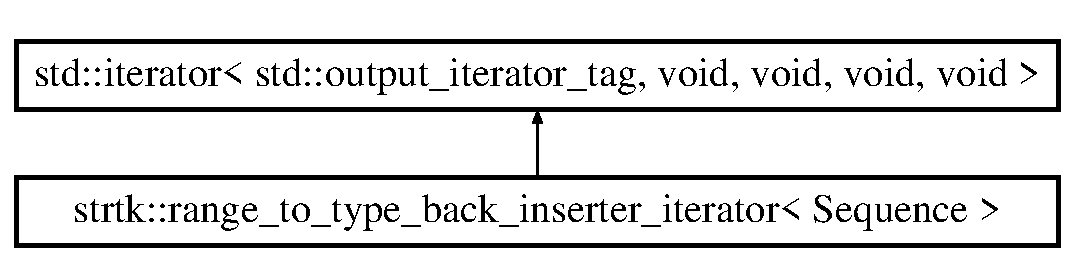
\includegraphics[height=2.000000cm]{classstrtk_1_1range__to__type__back__inserter__iterator}
\end{center}
\end{figure}
\subsection*{Public Types}
\begin{DoxyCompactItemize}
\item 
\hypertarget{classstrtk_1_1range__to__type__back__inserter__iterator_a9a297d1f94cc4e0862c0690c6972eb3a}{typedef Sequence\-::value\-\_\-type {\bfseries value\-\_\-type}}\label{classstrtk_1_1range__to__type__back__inserter__iterator_a9a297d1f94cc4e0862c0690c6972eb3a}

\end{DoxyCompactItemize}
\subsection*{Public Member Functions}
\begin{DoxyCompactItemize}
\item 
\hypertarget{classstrtk_1_1range__to__type__back__inserter__iterator_a667570a6686a54d36021adb22bd7e189}{{\bfseries range\-\_\-to\-\_\-type\-\_\-back\-\_\-inserter\-\_\-iterator} (Sequence \&sequence)}\label{classstrtk_1_1range__to__type__back__inserter__iterator_a667570a6686a54d36021adb22bd7e189}

\item 
\hypertarget{classstrtk_1_1range__to__type__back__inserter__iterator_ae83f6b4cb63e9b1c82bd429242e1e6d8}{{\bfseries range\-\_\-to\-\_\-type\-\_\-back\-\_\-inserter\-\_\-iterator} (const \hyperlink{classstrtk_1_1range__to__type__back__inserter__iterator}{range\-\_\-to\-\_\-type\-\_\-back\-\_\-inserter\-\_\-iterator} \&itr)}\label{classstrtk_1_1range__to__type__back__inserter__iterator_ae83f6b4cb63e9b1c82bd429242e1e6d8}

\item 
\hypertarget{classstrtk_1_1range__to__type__back__inserter__iterator_a7f3e029249f012a5d2b11c00c51b4d63}{\hyperlink{classstrtk_1_1range__to__type__back__inserter__iterator}{range\-\_\-to\-\_\-type\-\_\-back\-\_\-inserter\-\_\-iterator} \& {\bfseries operator=} (const \hyperlink{classstrtk_1_1range__to__type__back__inserter__iterator}{range\-\_\-to\-\_\-type\-\_\-back\-\_\-inserter\-\_\-iterator} \&itr)}\label{classstrtk_1_1range__to__type__back__inserter__iterator_a7f3e029249f012a5d2b11c00c51b4d63}

\item 
\hypertarget{classstrtk_1_1range__to__type__back__inserter__iterator_a7cdbe99e5555cdafb5f3077490fa2659}{{\footnotesize template$<$typename Iterator $>$ }\\\hyperlink{classstrtk_1_1range__to__type__back__inserter__iterator}{range\-\_\-to\-\_\-type\-\_\-back\-\_\-inserter\-\_\-iterator} \& {\bfseries operator=} (const std\-::pair$<$ Iterator, Iterator $>$ \&r)}\label{classstrtk_1_1range__to__type__back__inserter__iterator_a7cdbe99e5555cdafb5f3077490fa2659}

\item 
\hypertarget{classstrtk_1_1range__to__type__back__inserter__iterator_a55173efd60502915cdbcc53dfb2f3f88}{\hyperlink{classstrtk_1_1range__to__type__back__inserter__iterator}{range\-\_\-to\-\_\-type\-\_\-back\-\_\-inserter\-\_\-iterator} \& {\bfseries operator=} (const std\-::string \&s)}\label{classstrtk_1_1range__to__type__back__inserter__iterator_a55173efd60502915cdbcc53dfb2f3f88}

\item 
\hypertarget{classstrtk_1_1range__to__type__back__inserter__iterator_a6d38f9a9da571f42b83b7781615d8c77}{{\footnotesize template$<$typename Iterator $>$ }\\void {\bfseries operator()} (const std\-::pair$<$ Iterator, Iterator $>$ \&r) const }\label{classstrtk_1_1range__to__type__back__inserter__iterator_a6d38f9a9da571f42b83b7781615d8c77}

\item 
\hypertarget{classstrtk_1_1range__to__type__back__inserter__iterator_a958ac2dd68e0970fb984eb9beca3cd57}{{\footnotesize template$<$typename Iterator $>$ }\\void {\bfseries operator()} (const Iterator begin, const Iterator end)}\label{classstrtk_1_1range__to__type__back__inserter__iterator_a958ac2dd68e0970fb984eb9beca3cd57}

\item 
\hypertarget{classstrtk_1_1range__to__type__back__inserter__iterator_a15d28d30e968840abad54afd699849bc}{\hyperlink{classstrtk_1_1range__to__type__back__inserter__iterator}{range\-\_\-to\-\_\-type\-\_\-back\-\_\-inserter\-\_\-iterator} \& {\bfseries operator$\ast$} ()}\label{classstrtk_1_1range__to__type__back__inserter__iterator_a15d28d30e968840abad54afd699849bc}

\item 
\hypertarget{classstrtk_1_1range__to__type__back__inserter__iterator_ad198752ea500bf932039af509d4e733c}{\hyperlink{classstrtk_1_1range__to__type__back__inserter__iterator}{range\-\_\-to\-\_\-type\-\_\-back\-\_\-inserter\-\_\-iterator} \& {\bfseries operator++} ()}\label{classstrtk_1_1range__to__type__back__inserter__iterator_ad198752ea500bf932039af509d4e733c}

\item 
\hypertarget{classstrtk_1_1range__to__type__back__inserter__iterator_a50e260507ec04740cfdec09acdac6400}{\hyperlink{classstrtk_1_1range__to__type__back__inserter__iterator}{range\-\_\-to\-\_\-type\-\_\-back\-\_\-inserter\-\_\-iterator} {\bfseries operator++} (int)}\label{classstrtk_1_1range__to__type__back__inserter__iterator_a50e260507ec04740cfdec09acdac6400}

\end{DoxyCompactItemize}


The documentation for this class was generated from the following file\-:\begin{DoxyCompactItemize}
\item 
strtk.\-hpp\end{DoxyCompactItemize}

\hypertarget{classstrtk_1_1range__to__type__inserter__iterator}{\section{strtk\-:\-:range\-\_\-to\-\_\-type\-\_\-inserter\-\_\-iterator$<$ Set $>$ Class Template Reference}
\label{classstrtk_1_1range__to__type__inserter__iterator}\index{strtk\-::range\-\_\-to\-\_\-type\-\_\-inserter\-\_\-iterator$<$ Set $>$@{strtk\-::range\-\_\-to\-\_\-type\-\_\-inserter\-\_\-iterator$<$ Set $>$}}
}
Inheritance diagram for strtk\-:\-:range\-\_\-to\-\_\-type\-\_\-inserter\-\_\-iterator$<$ Set $>$\-:\begin{figure}[H]
\begin{center}
\leavevmode
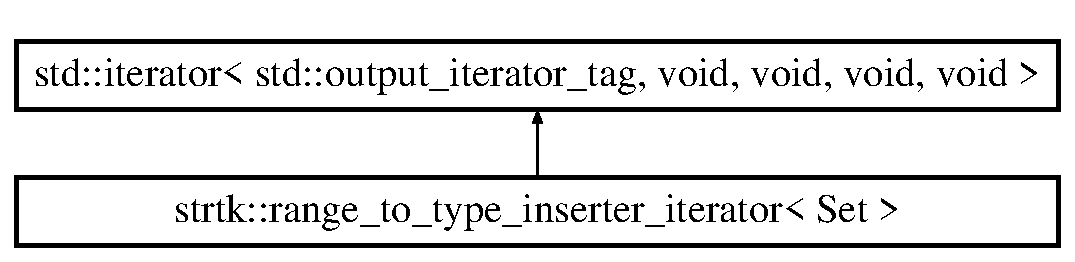
\includegraphics[height=2.000000cm]{classstrtk_1_1range__to__type__inserter__iterator}
\end{center}
\end{figure}
\subsection*{Public Types}
\begin{DoxyCompactItemize}
\item 
\hypertarget{classstrtk_1_1range__to__type__inserter__iterator_ab99a3748a8a9d1c9ae6b9f2fb3b4d094}{typedef Set\-::value\-\_\-type {\bfseries value\-\_\-type}}\label{classstrtk_1_1range__to__type__inserter__iterator_ab99a3748a8a9d1c9ae6b9f2fb3b4d094}

\end{DoxyCompactItemize}
\subsection*{Public Member Functions}
\begin{DoxyCompactItemize}
\item 
\hypertarget{classstrtk_1_1range__to__type__inserter__iterator_a28b9082fd9dea5b50b6995a8b11443df}{{\bfseries range\-\_\-to\-\_\-type\-\_\-inserter\-\_\-iterator} (Set \&set)}\label{classstrtk_1_1range__to__type__inserter__iterator_a28b9082fd9dea5b50b6995a8b11443df}

\item 
\hypertarget{classstrtk_1_1range__to__type__inserter__iterator_a77d490fec4aaf2a8c7dcca6f616aa7a2}{{\bfseries range\-\_\-to\-\_\-type\-\_\-inserter\-\_\-iterator} (const \hyperlink{classstrtk_1_1range__to__type__inserter__iterator}{range\-\_\-to\-\_\-type\-\_\-inserter\-\_\-iterator} \&itr)}\label{classstrtk_1_1range__to__type__inserter__iterator_a77d490fec4aaf2a8c7dcca6f616aa7a2}

\item 
\hypertarget{classstrtk_1_1range__to__type__inserter__iterator_a1efd479fd8afde7719eb540d11ead4ef}{\hyperlink{classstrtk_1_1range__to__type__inserter__iterator}{range\-\_\-to\-\_\-type\-\_\-inserter\-\_\-iterator} \& {\bfseries operator=} (const \hyperlink{classstrtk_1_1range__to__type__inserter__iterator}{range\-\_\-to\-\_\-type\-\_\-inserter\-\_\-iterator} \&itr)}\label{classstrtk_1_1range__to__type__inserter__iterator_a1efd479fd8afde7719eb540d11ead4ef}

\item 
\hypertarget{classstrtk_1_1range__to__type__inserter__iterator_a9c27a185f87ddc65f4315738fe65d417}{{\footnotesize template$<$typename Iterator $>$ }\\\hyperlink{classstrtk_1_1range__to__type__inserter__iterator}{range\-\_\-to\-\_\-type\-\_\-inserter\-\_\-iterator} \& {\bfseries operator=} (const std\-::pair$<$ Iterator, Iterator $>$ \&r)}\label{classstrtk_1_1range__to__type__inserter__iterator_a9c27a185f87ddc65f4315738fe65d417}

\item 
\hypertarget{classstrtk_1_1range__to__type__inserter__iterator_a1041f2cf6360a6e551507e40ec56fae3}{{\footnotesize template$<$typename Iterator $>$ }\\void {\bfseries operator()} (const std\-::pair$<$ Iterator, Iterator $>$ \&r)}\label{classstrtk_1_1range__to__type__inserter__iterator_a1041f2cf6360a6e551507e40ec56fae3}

\item 
\hypertarget{classstrtk_1_1range__to__type__inserter__iterator_affcee0aab400652427aeda5dbccb7924}{\hyperlink{classstrtk_1_1range__to__type__inserter__iterator}{range\-\_\-to\-\_\-type\-\_\-inserter\-\_\-iterator} \& {\bfseries operator$\ast$} ()}\label{classstrtk_1_1range__to__type__inserter__iterator_affcee0aab400652427aeda5dbccb7924}

\item 
\hypertarget{classstrtk_1_1range__to__type__inserter__iterator_a12dce4fc6cd8fbd47ba0aa4613d71a7b}{\hyperlink{classstrtk_1_1range__to__type__inserter__iterator}{range\-\_\-to\-\_\-type\-\_\-inserter\-\_\-iterator} \& {\bfseries operator++} ()}\label{classstrtk_1_1range__to__type__inserter__iterator_a12dce4fc6cd8fbd47ba0aa4613d71a7b}

\item 
\hypertarget{classstrtk_1_1range__to__type__inserter__iterator_aa377239a29af218a8afdd2e928d83310}{\hyperlink{classstrtk_1_1range__to__type__inserter__iterator}{range\-\_\-to\-\_\-type\-\_\-inserter\-\_\-iterator} {\bfseries operator++} (int)}\label{classstrtk_1_1range__to__type__inserter__iterator_aa377239a29af218a8afdd2e928d83310}

\end{DoxyCompactItemize}


The documentation for this class was generated from the following file\-:\begin{DoxyCompactItemize}
\item 
strtk.\-hpp\end{DoxyCompactItemize}

\hypertarget{classstrtk_1_1range__to__type__push__inserter__iterator}{\section{strtk\-:\-:range\-\_\-to\-\_\-type\-\_\-push\-\_\-inserter\-\_\-iterator$<$ Container $>$ Class Template Reference}
\label{classstrtk_1_1range__to__type__push__inserter__iterator}\index{strtk\-::range\-\_\-to\-\_\-type\-\_\-push\-\_\-inserter\-\_\-iterator$<$ Container $>$@{strtk\-::range\-\_\-to\-\_\-type\-\_\-push\-\_\-inserter\-\_\-iterator$<$ Container $>$}}
}
Inheritance diagram for strtk\-:\-:range\-\_\-to\-\_\-type\-\_\-push\-\_\-inserter\-\_\-iterator$<$ Container $>$\-:\begin{figure}[H]
\begin{center}
\leavevmode
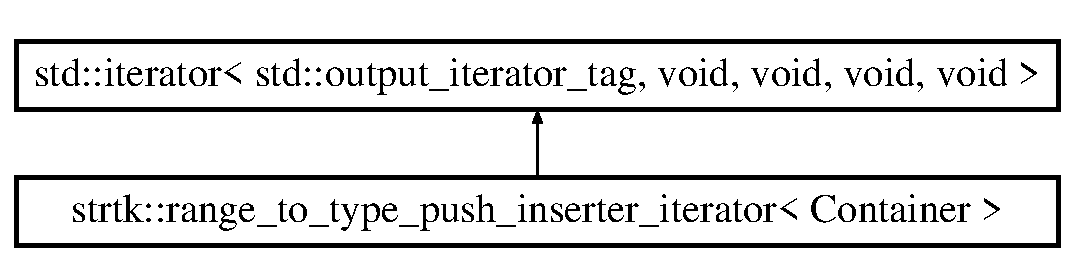
\includegraphics[height=2.000000cm]{classstrtk_1_1range__to__type__push__inserter__iterator}
\end{center}
\end{figure}
\subsection*{Public Types}
\begin{DoxyCompactItemize}
\item 
\hypertarget{classstrtk_1_1range__to__type__push__inserter__iterator_afae54a97ca5d5fb4c6fcb437eb1286f9}{typedef Container\-::value\-\_\-type {\bfseries value\-\_\-type}}\label{classstrtk_1_1range__to__type__push__inserter__iterator_afae54a97ca5d5fb4c6fcb437eb1286f9}

\end{DoxyCompactItemize}
\subsection*{Public Member Functions}
\begin{DoxyCompactItemize}
\item 
\hypertarget{classstrtk_1_1range__to__type__push__inserter__iterator_ae859fe59f86a18c1213cae54fdf4f30d}{{\bfseries range\-\_\-to\-\_\-type\-\_\-push\-\_\-inserter\-\_\-iterator} (Container \&container)}\label{classstrtk_1_1range__to__type__push__inserter__iterator_ae859fe59f86a18c1213cae54fdf4f30d}

\item 
\hypertarget{classstrtk_1_1range__to__type__push__inserter__iterator_aca654dcc9cc3d9b24ab1173eaa3976f5}{{\bfseries range\-\_\-to\-\_\-type\-\_\-push\-\_\-inserter\-\_\-iterator} (const \hyperlink{classstrtk_1_1range__to__type__push__inserter__iterator}{range\-\_\-to\-\_\-type\-\_\-push\-\_\-inserter\-\_\-iterator} \&itr)}\label{classstrtk_1_1range__to__type__push__inserter__iterator_aca654dcc9cc3d9b24ab1173eaa3976f5}

\item 
\hypertarget{classstrtk_1_1range__to__type__push__inserter__iterator_af8790c28e6739fe59b565767c6a258be}{\hyperlink{classstrtk_1_1range__to__type__push__inserter__iterator}{range\-\_\-to\-\_\-type\-\_\-push\-\_\-inserter\-\_\-iterator} \& {\bfseries operator=} (const \hyperlink{classstrtk_1_1range__to__type__push__inserter__iterator}{range\-\_\-to\-\_\-type\-\_\-push\-\_\-inserter\-\_\-iterator} \&itr)}\label{classstrtk_1_1range__to__type__push__inserter__iterator_af8790c28e6739fe59b565767c6a258be}

\item 
\hypertarget{classstrtk_1_1range__to__type__push__inserter__iterator_a6c431943f05857dafaa7e149b6a66041}{{\footnotesize template$<$typename Iterator $>$ }\\\hyperlink{classstrtk_1_1range__to__type__push__inserter__iterator}{range\-\_\-to\-\_\-type\-\_\-push\-\_\-inserter\-\_\-iterator} \& {\bfseries operator=} (const std\-::pair$<$ Iterator, Iterator $>$ \&r)}\label{classstrtk_1_1range__to__type__push__inserter__iterator_a6c431943f05857dafaa7e149b6a66041}

\item 
\hypertarget{classstrtk_1_1range__to__type__push__inserter__iterator_a62af013640a203f160b520630600340d}{{\footnotesize template$<$typename Iterator $>$ }\\void {\bfseries operator()} (const std\-::pair$<$ Iterator, Iterator $>$ \&r)}\label{classstrtk_1_1range__to__type__push__inserter__iterator_a62af013640a203f160b520630600340d}

\item 
\hypertarget{classstrtk_1_1range__to__type__push__inserter__iterator_a3f98f5df13dd951b57622fe609a0ce86}{\hyperlink{classstrtk_1_1range__to__type__push__inserter__iterator}{range\-\_\-to\-\_\-type\-\_\-push\-\_\-inserter\-\_\-iterator} \& {\bfseries operator$\ast$} ()}\label{classstrtk_1_1range__to__type__push__inserter__iterator_a3f98f5df13dd951b57622fe609a0ce86}

\item 
\hypertarget{classstrtk_1_1range__to__type__push__inserter__iterator_a90e9c11ace0790477e902d5b122ce63f}{\hyperlink{classstrtk_1_1range__to__type__push__inserter__iterator}{range\-\_\-to\-\_\-type\-\_\-push\-\_\-inserter\-\_\-iterator} \& {\bfseries operator++} ()}\label{classstrtk_1_1range__to__type__push__inserter__iterator_a90e9c11ace0790477e902d5b122ce63f}

\item 
\hypertarget{classstrtk_1_1range__to__type__push__inserter__iterator_ad96fda85234f520bf1a31da60e63e0c3}{\hyperlink{classstrtk_1_1range__to__type__push__inserter__iterator}{range\-\_\-to\-\_\-type\-\_\-push\-\_\-inserter\-\_\-iterator} {\bfseries operator++} (int)}\label{classstrtk_1_1range__to__type__push__inserter__iterator_ad96fda85234f520bf1a31da60e63e0c3}

\end{DoxyCompactItemize}


The documentation for this class was generated from the following file\-:\begin{DoxyCompactItemize}
\item 
strtk.\-hpp\end{DoxyCompactItemize}

\hypertarget{structstrtk_1_1details_1_1range__type}{\section{strtk\-:\-:details\-:\-:range\-\_\-type$<$ Iterator $>$ Struct Template Reference}
\label{structstrtk_1_1details_1_1range__type}\index{strtk\-::details\-::range\-\_\-type$<$ Iterator $>$@{strtk\-::details\-::range\-\_\-type$<$ Iterator $>$}}
}
\subsection*{Public Types}
\begin{DoxyCompactItemize}
\item 
\hypertarget{structstrtk_1_1details_1_1range__type_a33933b70fd000835a9a426b2815dc208}{typedef std\-::pair$<$ Iterator, \\*
Iterator $>$ {\bfseries type}}\label{structstrtk_1_1details_1_1range__type_a33933b70fd000835a9a426b2815dc208}

\end{DoxyCompactItemize}


The documentation for this struct was generated from the following file\-:\begin{DoxyCompactItemize}
\item 
strtk.\-hpp\end{DoxyCompactItemize}

\hypertarget{classstrtk_1_1binary_1_1reader}{\section{strtk\-:\-:binary\-:\-:reader Class Reference}
\label{classstrtk_1_1binary_1_1reader}\index{strtk\-::binary\-::reader@{strtk\-::binary\-::reader}}
}
\subsection*{Public Types}
\begin{DoxyCompactItemize}
\item 
\hypertarget{classstrtk_1_1binary_1_1reader_a878224e30c5be36f878dd15343d4f032}{typedef unsigned int {\bfseries uint32\-\_\-t}}\label{classstrtk_1_1binary_1_1reader_a878224e30c5be36f878dd15343d4f032}

\item 
\hypertarget{classstrtk_1_1binary_1_1reader_aa9814f877763e85063450ed021f0bd79}{typedef unsigned short {\bfseries uint16\-\_\-t}}\label{classstrtk_1_1binary_1_1reader_aa9814f877763e85063450ed021f0bd79}

\item 
\hypertarget{classstrtk_1_1binary_1_1reader_a39cf201b4b2c9afb0f8eba4b4378c224}{typedef unsigned char {\bfseries uint8\-\_\-t}}\label{classstrtk_1_1binary_1_1reader_a39cf201b4b2c9afb0f8eba4b4378c224}

\item 
\hypertarget{classstrtk_1_1binary_1_1reader_a840b0bd951884045986de7cdbce881c7}{typedef unsigned long long int {\bfseries uint64\-\_\-t}}\label{classstrtk_1_1binary_1_1reader_a840b0bd951884045986de7cdbce881c7}

\end{DoxyCompactItemize}
\subsection*{Public Member Functions}
\begin{DoxyCompactItemize}
\item 
\hypertarget{classstrtk_1_1binary_1_1reader_a45742996f92e8427315a86e4506d13bd}{{\footnotesize template$<$typename T $>$ }\\{\bfseries reader} (T $\ast$buffer, const std\-::size\-\_\-t \&buffer\-\_\-length)}\label{classstrtk_1_1binary_1_1reader_a45742996f92e8427315a86e4506d13bd}

\item 
\hypertarget{classstrtk_1_1binary_1_1reader_ad667e2fa0a8c4b956232c015f4195fb1}{bool {\bfseries operator!} () const }\label{classstrtk_1_1binary_1_1reader_ad667e2fa0a8c4b956232c015f4195fb1}

\item 
\hypertarget{classstrtk_1_1binary_1_1reader_a4730baa0d2576783eefc1b0a4f91d6ab}{void {\bfseries reset} (const bool clear\-\_\-buffer=false)}\label{classstrtk_1_1binary_1_1reader_a4730baa0d2576783eefc1b0a4f91d6ab}

\item 
\hypertarget{classstrtk_1_1binary_1_1reader_a591cd0d8a83fd91fe176c3a300235b16}{std\-::size\-\_\-t {\bfseries position} () const }\label{classstrtk_1_1binary_1_1reader_a591cd0d8a83fd91fe176c3a300235b16}

\item 
\hypertarget{classstrtk_1_1binary_1_1reader_a49ed4f2141cf741afcb82bfc9c18f8ac}{const char $\ast$ {\bfseries position\-\_\-ptr} () const }\label{classstrtk_1_1binary_1_1reader_a49ed4f2141cf741afcb82bfc9c18f8ac}

\item 
\hypertarget{classstrtk_1_1binary_1_1reader_a72e1a96be625c8d242ddd92c2a0db820}{std\-::size\-\_\-t {\bfseries amount\-\_\-read} ()}\label{classstrtk_1_1binary_1_1reader_a72e1a96be625c8d242ddd92c2a0db820}

\item 
\hypertarget{classstrtk_1_1binary_1_1reader_a0245de8d93c3a1f43a01d73e547d4f80}{bool {\bfseries rewind} (const std\-::size\-\_\-t \&n\-\_\-bytes)}\label{classstrtk_1_1binary_1_1reader_a0245de8d93c3a1f43a01d73e547d4f80}

\item 
\hypertarget{classstrtk_1_1binary_1_1reader_ae3e050128cf04fc9f8fe1b92c8ec2c86}{bool {\bfseries seek} (const int \&n\-\_\-bytes)}\label{classstrtk_1_1binary_1_1reader_ae3e050128cf04fc9f8fe1b92c8ec2c86}

\item 
\hypertarget{classstrtk_1_1binary_1_1reader_a85e7d176263e9813dbcff341aaf54e56}{void {\bfseries clear} ()}\label{classstrtk_1_1binary_1_1reader_a85e7d176263e9813dbcff341aaf54e56}

\item 
\hypertarget{classstrtk_1_1binary_1_1reader_aaad03496590bc097b823e519148f1994}{{\footnotesize template$<$typename T $>$ }\\bool {\bfseries operator()} (T $\ast$\&data, uint32\-\_\-t \&length, const bool read\-\_\-length=true)}\label{classstrtk_1_1binary_1_1reader_aaad03496590bc097b823e519148f1994}

\item 
\hypertarget{classstrtk_1_1binary_1_1reader_ab89714a751748c39d132311f53d936c7}{{\footnotesize template$<$typename T $>$ }\\bool {\bfseries operator()} (T $\ast$\&data, uint64\-\_\-t \&length, const bool read\-\_\-length=true)}\label{classstrtk_1_1binary_1_1reader_ab89714a751748c39d132311f53d936c7}

\item 
\hypertarget{classstrtk_1_1binary_1_1reader_a7f1dacb25a8b0ba8bb047f00c5309365}{bool {\bfseries operator()} (std\-::string \&output)}\label{classstrtk_1_1binary_1_1reader_a7f1dacb25a8b0ba8bb047f00c5309365}

\item 
\hypertarget{classstrtk_1_1binary_1_1reader_a435d4cec43c5a9902da0505f6c7243ed}{{\footnotesize template$<$typename T1 , typename T2 $>$ }\\bool {\bfseries operator()} (std\-::pair$<$ T1, T2 $>$ \&p)}\label{classstrtk_1_1binary_1_1reader_a435d4cec43c5a9902da0505f6c7243ed}

\item 
\hypertarget{classstrtk_1_1binary_1_1reader_adc5fb4d93ff892664b5269a42cdd8ea4}{{\footnotesize template$<$typename T , typename Allocator , template$<$ typename, typename $>$ class Sequence$>$ }\\bool {\bfseries operator()} (Sequence$<$ T, Allocator $>$ \&seq)}\label{classstrtk_1_1binary_1_1reader_adc5fb4d93ff892664b5269a42cdd8ea4}

\item 
\hypertarget{classstrtk_1_1binary_1_1reader_ae52a575bf3f36dd642ef682861479370}{{\footnotesize template$<$typename T , typename Allocator $>$ }\\bool {\bfseries operator()} (std\-::vector$<$ T, Allocator $>$ \&vec)}\label{classstrtk_1_1binary_1_1reader_ae52a575bf3f36dd642ef682861479370}

\item 
\hypertarget{classstrtk_1_1binary_1_1reader_a147964977914bd343d11c4a2b18523a2}{{\footnotesize template$<$typename T , typename Comparator , typename Allocator $>$ }\\bool {\bfseries operator()} (std\-::set$<$ T, Comparator, Allocator $>$ \&set)}\label{classstrtk_1_1binary_1_1reader_a147964977914bd343d11c4a2b18523a2}

\item 
\hypertarget{classstrtk_1_1binary_1_1reader_a2df4318d301c74d710a2554a71f8309b}{{\footnotesize template$<$typename T , typename Allocator , typename Comparator $>$ }\\bool {\bfseries operator()} (std\-::multiset$<$ T, Allocator, Comparator $>$ \&multiset)}\label{classstrtk_1_1binary_1_1reader_a2df4318d301c74d710a2554a71f8309b}

\item 
\hypertarget{classstrtk_1_1binary_1_1reader_a55dd49958fecb7e9e14beea8fe34939b}{bool {\bfseries operator()} (std\-::ifstream \&stream, const std\-::size\-\_\-t \&length)}\label{classstrtk_1_1binary_1_1reader_a55dd49958fecb7e9e14beea8fe34939b}

\item 
\hypertarget{classstrtk_1_1binary_1_1reader_a0a21eab78cea0b224add5897adf58035}{bool {\bfseries operator()} (std\-::ifstream \&stream)}\label{classstrtk_1_1binary_1_1reader_a0a21eab78cea0b224add5897adf58035}

\item 
\hypertarget{classstrtk_1_1binary_1_1reader_ab5440c08282f2e8ee6922ed1ba38aa3f}{{\footnotesize template$<$typename T $>$ }\\bool {\bfseries operator()} (T \&output)}\label{classstrtk_1_1binary_1_1reader_ab5440c08282f2e8ee6922ed1ba38aa3f}

\item 
\hypertarget{classstrtk_1_1binary_1_1reader_a0c0c3d6afbe4fa52497cdcda779c4348}{{\footnotesize template$<$typename T $>$ }\\bool {\bfseries operator()} (const T \&output)}\label{classstrtk_1_1binary_1_1reader_a0c0c3d6afbe4fa52497cdcda779c4348}

\item 
\hypertarget{classstrtk_1_1binary_1_1reader_a6f293e7966fe6b4777b0a99ab96b8980}{{\footnotesize template$<$typename T $>$ }\\bool {\bfseries be\-\_\-to\-\_\-native} (T \&output)}\label{classstrtk_1_1binary_1_1reader_a6f293e7966fe6b4777b0a99ab96b8980}

\item 
\hypertarget{classstrtk_1_1binary_1_1reader_ae48dbc44422b1da0b25b7c3ff464cacd}{{\footnotesize template$<$typename T $>$ }\\bool {\bfseries le\-\_\-to\-\_\-native} (T \&output)}\label{classstrtk_1_1binary_1_1reader_ae48dbc44422b1da0b25b7c3ff464cacd}

\item 
\hypertarget{classstrtk_1_1binary_1_1reader_a36b4317b42c9889b6066ed7728f0c1cf}{{\footnotesize template$<$typename T , std\-::size\-\_\-t N$>$ }\\bool {\bfseries operator()} (T(\&output)\mbox{[}N\mbox{]})}\label{classstrtk_1_1binary_1_1reader_a36b4317b42c9889b6066ed7728f0c1cf}

\item 
\hypertarget{classstrtk_1_1binary_1_1reader_a4944efd16c67e6f2bdc35ee2f97b9ab4}{{\footnotesize template$<$typename T $>$ }\\bool {\bfseries operator()} (T \&output, const std\-::size\-\_\-t \&size)}\label{classstrtk_1_1binary_1_1reader_a4944efd16c67e6f2bdc35ee2f97b9ab4}

\item 
\hypertarget{classstrtk_1_1binary_1_1reader_aebd3667fe3e2e376be127795b71c21e8}{void {\bfseries mark} ()}\label{classstrtk_1_1binary_1_1reader_aebd3667fe3e2e376be127795b71c21e8}

\item 
\hypertarget{classstrtk_1_1binary_1_1reader_a3ef883aae38e2f3e8d1ecc4b61ee3363}{bool {\bfseries reset\-\_\-to\-\_\-mark} ()}\label{classstrtk_1_1binary_1_1reader_a3ef883aae38e2f3e8d1ecc4b61ee3363}

\end{DoxyCompactItemize}


The documentation for this class was generated from the following file\-:\begin{DoxyCompactItemize}
\item 
strtk.\-hpp\end{DoxyCompactItemize}

\hypertarget{structstrtk_1_1details_1_1real__type}{\section{strtk\-:\-:details\-:\-:real\-\_\-type$<$ Real\-Type $>$ Struct Template Reference}
\label{structstrtk_1_1details_1_1real__type}\index{strtk\-::details\-::real\-\_\-type$<$ Real\-Type $>$@{strtk\-::details\-::real\-\_\-type$<$ Real\-Type $>$}}
}


The documentation for this struct was generated from the following file\-:\begin{DoxyCompactItemize}
\item 
strtk.\-hpp\end{DoxyCompactItemize}

\hypertarget{structstrtk_1_1details_1_1real__type_3_01double_01_4}{\section{strtk\-:\-:details\-:\-:real\-\_\-type$<$ double $>$ Struct Template Reference}
\label{structstrtk_1_1details_1_1real__type_3_01double_01_4}\index{strtk\-::details\-::real\-\_\-type$<$ double $>$@{strtk\-::details\-::real\-\_\-type$<$ double $>$}}
}
\subsection*{Public Types}
\begin{DoxyCompactItemize}
\item 
\hypertarget{structstrtk_1_1details_1_1real__type_3_01double_01_4_a1802b336e2049fca08d2b398802765d3}{typedef double {\bfseries type}}\label{structstrtk_1_1details_1_1real__type_3_01double_01_4_a1802b336e2049fca08d2b398802765d3}

\end{DoxyCompactItemize}


The documentation for this struct was generated from the following file\-:\begin{DoxyCompactItemize}
\item 
strtk.\-hpp\end{DoxyCompactItemize}

\hypertarget{structstrtk_1_1details_1_1real__type_3_01float_01_4}{\section{strtk\-:\-:details\-:\-:real\-\_\-type$<$ float $>$ Struct Template Reference}
\label{structstrtk_1_1details_1_1real__type_3_01float_01_4}\index{strtk\-::details\-::real\-\_\-type$<$ float $>$@{strtk\-::details\-::real\-\_\-type$<$ float $>$}}
}
\subsection*{Public Types}
\begin{DoxyCompactItemize}
\item 
\hypertarget{structstrtk_1_1details_1_1real__type_3_01float_01_4_a821fdbee30fb0fbca75d97581e1d291e}{typedef double {\bfseries type}}\label{structstrtk_1_1details_1_1real__type_3_01float_01_4_a821fdbee30fb0fbca75d97581e1d291e}

\end{DoxyCompactItemize}


The documentation for this struct was generated from the following file\-:\begin{DoxyCompactItemize}
\item 
strtk.\-hpp\end{DoxyCompactItemize}

\hypertarget{structstrtk_1_1details_1_1real__type_3_01long_01double_01_4}{\section{strtk\-:\-:details\-:\-:real\-\_\-type$<$ long double $>$ Struct Template Reference}
\label{structstrtk_1_1details_1_1real__type_3_01long_01double_01_4}\index{strtk\-::details\-::real\-\_\-type$<$ long double $>$@{strtk\-::details\-::real\-\_\-type$<$ long double $>$}}
}
\subsection*{Public Types}
\begin{DoxyCompactItemize}
\item 
\hypertarget{structstrtk_1_1details_1_1real__type_3_01long_01double_01_4_a48ff0d17fae2b2d58e5968f76d2fbdb3}{typedef long double {\bfseries type}}\label{structstrtk_1_1details_1_1real__type_3_01long_01double_01_4_a48ff0d17fae2b2d58e5968f76d2fbdb3}

\end{DoxyCompactItemize}


The documentation for this struct was generated from the following file\-:\begin{DoxyCompactItemize}
\item 
strtk.\-hpp\end{DoxyCompactItemize}

\hypertarget{structstrtk_1_1details_1_1real__type__tag}{\section{strtk\-:\-:details\-:\-:real\-\_\-type\-\_\-tag Struct Reference}
\label{structstrtk_1_1details_1_1real__type__tag}\index{strtk\-::details\-::real\-\_\-type\-\_\-tag@{strtk\-::details\-::real\-\_\-type\-\_\-tag}}
}


The documentation for this struct was generated from the following file\-:\begin{DoxyCompactItemize}
\item 
strtk.\-hpp\end{DoxyCompactItemize}

\hypertarget{structstrtk_1_1token__grid_1_1store_1_1remove__column__impl}{\section{strtk\-:\-:token\-\_\-grid\-:\-:store\-:\-:remove\-\_\-column\-\_\-impl Struct Reference}
\label{structstrtk_1_1token__grid_1_1store_1_1remove__column__impl}\index{strtk\-::token\-\_\-grid\-::store\-::remove\-\_\-column\-\_\-impl@{strtk\-::token\-\_\-grid\-::store\-::remove\-\_\-column\-\_\-impl}}
}
\subsection*{Public Member Functions}
\begin{DoxyCompactItemize}
\item 
\hypertarget{structstrtk_1_1token__grid_1_1store_1_1remove__column__impl_ab8c202f649b03e757fda440d9bf4677f}{void {\bfseries update} (store \&idx)}\label{structstrtk_1_1token__grid_1_1store_1_1remove__column__impl_ab8c202f649b03e757fda440d9bf4677f}

\item 
\hypertarget{structstrtk_1_1token__grid_1_1store_1_1remove__column__impl_a46b2200bc04cd826213519487484dee0}{void {\bfseries process} (store \&idx)}\label{structstrtk_1_1token__grid_1_1store_1_1remove__column__impl_a46b2200bc04cd826213519487484dee0}

\end{DoxyCompactItemize}
\subsection*{Public Attributes}
\begin{DoxyCompactItemize}
\item 
\hypertarget{structstrtk_1_1token__grid_1_1store_1_1remove__column__impl_a8caec52a8a931cdf22e177da5575ebb6}{std\-::size\-\_\-t {\bfseries column}}\label{structstrtk_1_1token__grid_1_1store_1_1remove__column__impl_a8caec52a8a931cdf22e177da5575ebb6}

\item 
\hypertarget{structstrtk_1_1token__grid_1_1store_1_1remove__column__impl_a13d21677fb89d1684630048c60b12d8e}{std\-::size\-\_\-t {\bfseries counter}}\label{structstrtk_1_1token__grid_1_1store_1_1remove__column__impl_a13d21677fb89d1684630048c60b12d8e}

\item 
\hypertarget{structstrtk_1_1token__grid_1_1store_1_1remove__column__impl_ad292ad299ed344f77ea48beced6ae5ed}{std\-::size\-\_\-t {\bfseries remainder}}\label{structstrtk_1_1token__grid_1_1store_1_1remove__column__impl_ad292ad299ed344f77ea48beced6ae5ed}

\item 
\hypertarget{structstrtk_1_1token__grid_1_1store_1_1remove__column__impl_a39de5406d4acd7286637ecb870cb5728}{std\-::size\-\_\-t {\bfseries current\-\_\-row}}\label{structstrtk_1_1token__grid_1_1store_1_1remove__column__impl_a39de5406d4acd7286637ecb870cb5728}

\end{DoxyCompactItemize}


The documentation for this struct was generated from the following file\-:\begin{DoxyCompactItemize}
\item 
strtk.\-hpp\end{DoxyCompactItemize}

\hypertarget{classresults}{\section{results Class Reference}
\label{classresults}\index{results@{results}}
}
\subsection*{Public Member Functions}
\begin{DoxyCompactItemize}
\item 
\hypertarget{classresults_a0e4d38b1a41064d0eef3b39290d459c2}{void {\bfseries add} (\hyperlink{classFileRecord}{File\-Record} $\ast$, double)}\label{classresults_a0e4d38b1a41064d0eef3b39290d459c2}

\item 
\hypertarget{classresults_abe3d7a331a246efc7e045c6f4b4677f8}{\hyperlink{classresults}{results} $\ast$ {\bfseries A\-N\-D} (\hyperlink{classresults}{results} $\ast$)}\label{classresults_abe3d7a331a246efc7e045c6f4b4677f8}

\item 
\hypertarget{classresults_aaca7df4883d9d88a7ec97d1cac63ad39}{\hyperlink{classresults}{results} $\ast$ {\bfseries O\-R} (\hyperlink{classresults}{results} $\ast$)}\label{classresults_aaca7df4883d9d88a7ec97d1cac63ad39}

\item 
\hypertarget{classresults_a2da077526ccff5d479e9a9ddd2696296}{\hyperlink{classresults}{results} $\ast$ {\bfseries N\-O\-T} (\hyperlink{classresults}{results} $\ast$)}\label{classresults_a2da077526ccff5d479e9a9ddd2696296}

\item 
\hypertarget{classresults_a0aea048dfe8abd06a61d8880c8db58a0}{\hyperlink{classresults}{results} $\ast$ {\bfseries display} ()}\label{classresults_a0aea048dfe8abd06a61d8880c8db58a0}

\item 
\hypertarget{classresults_ad820ad21c5368fcc381233626f166b38}{void {\bfseries openresult} (int)}\label{classresults_ad820ad21c5368fcc381233626f166b38}

\end{DoxyCompactItemize}


The documentation for this class was generated from the following files\-:\begin{DoxyCompactItemize}
\item 
results.\-h\item 
results.\-cpp\end{DoxyCompactItemize}

\hypertarget{classstrtk_1_1token__grid_1_1row__type}{\section{strtk\-:\-:token\-\_\-grid\-:\-:row\-\_\-type Class Reference}
\label{classstrtk_1_1token__grid_1_1row__type}\index{strtk\-::token\-\_\-grid\-::row\-\_\-type@{strtk\-::token\-\_\-grid\-::row\-\_\-type}}
}
\subsection*{Public Member Functions}
\begin{DoxyCompactItemize}
\item 
\hypertarget{classstrtk_1_1token__grid_1_1row__type_a56f138d13100bda1afa61a4979a02e21}{{\bfseries row\-\_\-type} (const std\-::size\-\_\-t \&index, const store \&dsv\-\_\-index)}\label{classstrtk_1_1token__grid_1_1row__type_a56f138d13100bda1afa61a4979a02e21}

\item 
\hypertarget{classstrtk_1_1token__grid_1_1row__type_aa823e12f7aea422bcb63906ad2f8759d}{bool {\bfseries is\-\_\-null} (const std\-::size\-\_\-t \&index) const }\label{classstrtk_1_1token__grid_1_1row__type_aa823e12f7aea422bcb63906ad2f8759d}

\item 
\hypertarget{classstrtk_1_1token__grid_1_1row__type_a1214525f909f85a07168c1b143cfa290}{{\footnotesize template$<$typename T $>$ }\\T {\bfseries operator\mbox{[}$\,$\mbox{]}} (const std\-::size\-\_\-t \&index) const }\label{classstrtk_1_1token__grid_1_1row__type_a1214525f909f85a07168c1b143cfa290}

\item 
\hypertarget{classstrtk_1_1token__grid_1_1row__type_a68872f83287df823e7a242ef4472c4ae}{{\footnotesize template$<$typename T $>$ }\\T {\bfseries get} (const std\-::size\-\_\-t \&index) const }\label{classstrtk_1_1token__grid_1_1row__type_a68872f83287df823e7a242ef4472c4ae}

\item 
\hypertarget{classstrtk_1_1token__grid_1_1row__type_a76c620f9867e214a5ab39e613c8d3396}{col\-\_\-range\-\_\-t {\bfseries all\-\_\-columns} () const }\label{classstrtk_1_1token__grid_1_1row__type_a76c620f9867e214a5ab39e613c8d3396}

\item 
\hypertarget{classstrtk_1_1token__grid_1_1row__type_a8902d09b9dc83034ea3fbca61e4be868}{range\-\_\-t {\bfseries range} () const }\label{classstrtk_1_1token__grid_1_1row__type_a8902d09b9dc83034ea3fbca61e4be868}

\item 
\hypertarget{classstrtk_1_1token__grid_1_1row__type_a599f1961841bd4d0cb494ef10a81b5fa}{range\-\_\-t {\bfseries token} (const std\-::size\-\_\-t \&index) const }\label{classstrtk_1_1token__grid_1_1row__type_a599f1961841bd4d0cb494ef10a81b5fa}

\item 
\hypertarget{classstrtk_1_1token__grid_1_1row__type_a8b67bc1789b49cd27d018c43f70afcc8}{std\-::size\-\_\-t {\bfseries index} () const }\label{classstrtk_1_1token__grid_1_1row__type_a8b67bc1789b49cd27d018c43f70afcc8}

\item 
\hypertarget{classstrtk_1_1token__grid_1_1row__type_ab4dc016699cd2f77ec0e453e106eaf49}{std\-::size\-\_\-t {\bfseries size} () const }\label{classstrtk_1_1token__grid_1_1row__type_ab4dc016699cd2f77ec0e453e106eaf49}

\item 
\hypertarget{classstrtk_1_1token__grid_1_1row__type_afc06c4d4163128352c4ac8b0d293b002}{std\-::size\-\_\-t {\bfseries raw\-\_\-length} () const }\label{classstrtk_1_1token__grid_1_1row__type_afc06c4d4163128352c4ac8b0d293b002}

\item 
\hypertarget{classstrtk_1_1token__grid_1_1row__type_a68aadd95c3a77fa93c8edbfdaa07f364}{std\-::size\-\_\-t {\bfseries raw\-\_\-length} (const std\-::size\-\_\-t \&column\-\_\-index) const }\label{classstrtk_1_1token__grid_1_1row__type_a68aadd95c3a77fa93c8edbfdaa07f364}

\item 
\hypertarget{classstrtk_1_1token__grid_1_1row__type_aa370a115f8b964d43d666808ed99f9f8}{std\-::string {\bfseries as\-\_\-string} () const }\label{classstrtk_1_1token__grid_1_1row__type_aa370a115f8b964d43d666808ed99f9f8}

\item 
\hypertarget{classstrtk_1_1token__grid_1_1row__type_a8b949555004ed6ff7e09ee25ce90c43a}{void {\bfseries as\-\_\-string} (std\-::string \&out) const }\label{classstrtk_1_1token__grid_1_1row__type_a8b949555004ed6ff7e09ee25ce90c43a}

\item 
\hypertarget{classstrtk_1_1token__grid_1_1row__type_a8836f04ba541110aaf90b40f4e42f2df}{{\footnotesize template$<$typename T0 , typename T1 , typename T2 , typename T3 , typename T4 , typename T5 , typename T6 , typename T7 , typename T8 , typename T9 $>$ }\\bool {\bfseries parse\-\_\-with\-\_\-index} (const std\-::size\-\_\-t \&col0, const std\-::size\-\_\-t \&col1, const std\-::size\-\_\-t \&col2, const std\-::size\-\_\-t \&col3, const std\-::size\-\_\-t \&col4, const std\-::size\-\_\-t \&col5, const std\-::size\-\_\-t \&col6, const std\-::size\-\_\-t \&col7, const std\-::size\-\_\-t \&col8, const std\-::size\-\_\-t \&col9, T0 \&t0, T1 \&t1, T2 \&t2, T3 \&t3, T4 \&t4, T5 \&t5, T6 \&t6, T7 \&t7, T8 \&t8, T9 \&t9) const }\label{classstrtk_1_1token__grid_1_1row__type_a8836f04ba541110aaf90b40f4e42f2df}

\item 
\hypertarget{classstrtk_1_1token__grid_1_1row__type_a84fc2aa7bea78e1ecc3b99bcdfbd7d9d}{{\footnotesize template$<$typename T0 , typename T1 , typename T2 , typename T3 , typename T4 , typename T5 , typename T6 , typename T7 , typename T8 $>$ }\\bool {\bfseries parse\-\_\-with\-\_\-index} (const std\-::size\-\_\-t \&col0, const std\-::size\-\_\-t \&col1, const std\-::size\-\_\-t \&col2, const std\-::size\-\_\-t \&col3, const std\-::size\-\_\-t \&col4, const std\-::size\-\_\-t \&col5, const std\-::size\-\_\-t \&col6, const std\-::size\-\_\-t \&col7, const std\-::size\-\_\-t \&col8, T0 \&t0, T1 \&t1, T2 \&t2, T3 \&t3, T4 \&t4, T5 \&t5, T6 \&t6, T7 \&t7, T8 \&t8) const }\label{classstrtk_1_1token__grid_1_1row__type_a84fc2aa7bea78e1ecc3b99bcdfbd7d9d}

\item 
\hypertarget{classstrtk_1_1token__grid_1_1row__type_a1f6179df2fa5247e7a36e2e0c3c2e042}{{\footnotesize template$<$typename T0 , typename T1 , typename T2 , typename T3 , typename T4 , typename T5 , typename T6 , typename T7 $>$ }\\bool {\bfseries parse\-\_\-with\-\_\-index} (const std\-::size\-\_\-t \&col0, const std\-::size\-\_\-t \&col1, const std\-::size\-\_\-t \&col2, const std\-::size\-\_\-t \&col3, const std\-::size\-\_\-t \&col4, const std\-::size\-\_\-t \&col5, const std\-::size\-\_\-t \&col6, const std\-::size\-\_\-t \&col7, T0 \&t0, T1 \&t1, T2 \&t2, T3 \&t3, T4 \&t4, T5 \&t5, T6 \&t6, T7 \&t7) const }\label{classstrtk_1_1token__grid_1_1row__type_a1f6179df2fa5247e7a36e2e0c3c2e042}

\item 
\hypertarget{classstrtk_1_1token__grid_1_1row__type_aa546694dacbe71bf31cd42925f39a0b9}{{\footnotesize template$<$typename T0 , typename T1 , typename T2 , typename T3 , typename T4 , typename T5 , typename T6 $>$ }\\bool {\bfseries parse\-\_\-with\-\_\-index} (const std\-::size\-\_\-t \&col0, const std\-::size\-\_\-t \&col1, const std\-::size\-\_\-t \&col2, const std\-::size\-\_\-t \&col3, const std\-::size\-\_\-t \&col4, const std\-::size\-\_\-t \&col5, const std\-::size\-\_\-t \&col6, T0 \&t0, T1 \&t1, T2 \&t2, T3 \&t3, T4 \&t4, T5 \&t5, T6 \&t6) const }\label{classstrtk_1_1token__grid_1_1row__type_aa546694dacbe71bf31cd42925f39a0b9}

\item 
\hypertarget{classstrtk_1_1token__grid_1_1row__type_ab0a3c00a32f9761d727fd9112518cd82}{{\footnotesize template$<$typename T0 , typename T1 , typename T2 , typename T3 , typename T4 , typename T5 $>$ }\\bool {\bfseries parse\-\_\-with\-\_\-index} (const std\-::size\-\_\-t \&col0, const std\-::size\-\_\-t \&col1, const std\-::size\-\_\-t \&col2, const std\-::size\-\_\-t \&col3, const std\-::size\-\_\-t \&col4, const std\-::size\-\_\-t \&col5, T0 \&t0, T1 \&t1, T2 \&t2, T3 \&t3, T4 \&t4, T5 \&t5) const }\label{classstrtk_1_1token__grid_1_1row__type_ab0a3c00a32f9761d727fd9112518cd82}

\item 
\hypertarget{classstrtk_1_1token__grid_1_1row__type_af5b9963352e66a72854b9039c022a8e7}{{\footnotesize template$<$typename T0 , typename T1 , typename T2 , typename T3 , typename T4 $>$ }\\bool {\bfseries parse\-\_\-with\-\_\-index} (const std\-::size\-\_\-t \&col0, const std\-::size\-\_\-t \&col1, const std\-::size\-\_\-t \&col2, const std\-::size\-\_\-t \&col3, const std\-::size\-\_\-t \&col4, T0 \&t0, T1 \&t1, T2 \&t2, T3 \&t3, T4 \&t4) const }\label{classstrtk_1_1token__grid_1_1row__type_af5b9963352e66a72854b9039c022a8e7}

\item 
\hypertarget{classstrtk_1_1token__grid_1_1row__type_a6491a1bb4f51a6bbdb538df8d832f332}{{\footnotesize template$<$typename T0 , typename T1 , typename T2 , typename T3 $>$ }\\bool {\bfseries parse\-\_\-with\-\_\-index} (const std\-::size\-\_\-t \&col0, const std\-::size\-\_\-t \&col1, const std\-::size\-\_\-t \&col2, const std\-::size\-\_\-t \&col3, T0 \&t0, T1 \&t1, T2 \&t2, T3 \&t3) const }\label{classstrtk_1_1token__grid_1_1row__type_a6491a1bb4f51a6bbdb538df8d832f332}

\item 
\hypertarget{classstrtk_1_1token__grid_1_1row__type_a1cdce192085e21cd6e8718ed8507f8f4}{{\footnotesize template$<$typename T0 , typename T1 , typename T2 $>$ }\\bool {\bfseries parse\-\_\-with\-\_\-index} (const std\-::size\-\_\-t \&col0, const std\-::size\-\_\-t \&col1, const std\-::size\-\_\-t \&col2, T0 \&t0, T1 \&t1, T2 \&t2) const }\label{classstrtk_1_1token__grid_1_1row__type_a1cdce192085e21cd6e8718ed8507f8f4}

\item 
\hypertarget{classstrtk_1_1token__grid_1_1row__type_a0108b3133bec89ad8741f4738e55725a}{{\footnotesize template$<$typename T0 , typename T1 $>$ }\\bool {\bfseries parse\-\_\-with\-\_\-index} (const std\-::size\-\_\-t \&col0, const std\-::size\-\_\-t \&col1, T0 \&t0, T1 \&t1) const }\label{classstrtk_1_1token__grid_1_1row__type_a0108b3133bec89ad8741f4738e55725a}

\item 
\hypertarget{classstrtk_1_1token__grid_1_1row__type_a76ff35559b95196da7d0e2ace76155cf}{{\footnotesize template$<$typename T $>$ }\\bool {\bfseries parse\-\_\-with\-\_\-index} (const std\-::size\-\_\-t \&col, T \&t) const }\label{classstrtk_1_1token__grid_1_1row__type_a76ff35559b95196da7d0e2ace76155cf}

\item 
\hypertarget{classstrtk_1_1token__grid_1_1row__type_aad471c6de83869088dcda881250123b8}{{\footnotesize template$<$typename T0 , typename T1 , typename T2 , typename T3 , typename T4 , typename T5 , typename T6 , typename T7 , typename T8 , typename T9 $>$ }\\bool {\bfseries parse} (T0 \&t0, T1 \&t1, T2 \&t2, T3 \&t3, T4 \&t4, T5 \&t5, T6 \&t6, T7 \&t7, T8 \&t8, T9 \&t9) const }\label{classstrtk_1_1token__grid_1_1row__type_aad471c6de83869088dcda881250123b8}

\item 
\hypertarget{classstrtk_1_1token__grid_1_1row__type_ae24e3a18699ea19d410181978874171d}{{\footnotesize template$<$typename T0 , typename T1 , typename T2 , typename T3 , typename T4 , typename T5 , typename T6 , typename T7 , typename T8 $>$ }\\bool {\bfseries parse} (T0 \&t0, T1 \&t1, T2 \&t2, T3 \&t3, T4 \&t4, T5 \&t5, T6 \&t6, T7 \&t7, T8 \&t8) const }\label{classstrtk_1_1token__grid_1_1row__type_ae24e3a18699ea19d410181978874171d}

\item 
\hypertarget{classstrtk_1_1token__grid_1_1row__type_a5e8d1e7ffad0ba35130364450ed782b8}{{\footnotesize template$<$typename T0 , typename T1 , typename T2 , typename T3 , typename T4 , typename T5 , typename T6 , typename T7 $>$ }\\bool {\bfseries parse} (T0 \&t0, T1 \&t1, T2 \&t2, T3 \&t3, T4 \&t4, T5 \&t5, T6 \&t6, T7 \&t7) const }\label{classstrtk_1_1token__grid_1_1row__type_a5e8d1e7ffad0ba35130364450ed782b8}

\item 
\hypertarget{classstrtk_1_1token__grid_1_1row__type_a294c52872e3e2e5c62a77b5231c8669a}{{\footnotesize template$<$typename T0 , typename T1 , typename T2 , typename T3 , typename T4 , typename T5 , typename T6 $>$ }\\bool {\bfseries parse} (T0 \&t0, T1 \&t1, T2 \&t2, T3 \&t3, T4 \&t4, T5 \&t5, T6 \&t6) const }\label{classstrtk_1_1token__grid_1_1row__type_a294c52872e3e2e5c62a77b5231c8669a}

\item 
\hypertarget{classstrtk_1_1token__grid_1_1row__type_ac957a38f1b6c1e808fb3c5051b937575}{{\footnotesize template$<$typename T0 , typename T1 , typename T2 , typename T3 , typename T4 , typename T5 $>$ }\\bool {\bfseries parse} (T0 \&t0, T1 \&t1, T2 \&t2, T3 \&t3, T4 \&t4, T5 \&t5) const }\label{classstrtk_1_1token__grid_1_1row__type_ac957a38f1b6c1e808fb3c5051b937575}

\item 
\hypertarget{classstrtk_1_1token__grid_1_1row__type_ae5539369ee3f93620a0193a8b80cbadd}{{\footnotesize template$<$typename T0 , typename T1 , typename T2 , typename T3 , typename T4 $>$ }\\bool {\bfseries parse} (T0 \&t0, T1 \&t1, T2 \&t2, T3 \&t3, T4 \&t4) const }\label{classstrtk_1_1token__grid_1_1row__type_ae5539369ee3f93620a0193a8b80cbadd}

\item 
\hypertarget{classstrtk_1_1token__grid_1_1row__type_a5dc6fea536f990f2cf622a2f46954b85}{{\footnotesize template$<$typename T0 , typename T1 , typename T2 , typename T3 $>$ }\\bool {\bfseries parse} (T0 \&t0, T1 \&t1, T2 \&t2, T3 \&t3) const }\label{classstrtk_1_1token__grid_1_1row__type_a5dc6fea536f990f2cf622a2f46954b85}

\item 
\hypertarget{classstrtk_1_1token__grid_1_1row__type_ad6f18423cd68f6435cf9534ecbf95228}{{\footnotesize template$<$typename T0 , typename T1 , typename T2 $>$ }\\bool {\bfseries parse} (T0 \&t0, T1 \&t1, T2 \&t2) const }\label{classstrtk_1_1token__grid_1_1row__type_ad6f18423cd68f6435cf9534ecbf95228}

\item 
\hypertarget{classstrtk_1_1token__grid_1_1row__type_a80345e2864f97a53b5cf55039e4ef624}{{\footnotesize template$<$typename T0 , typename T1 $>$ }\\bool {\bfseries parse} (T0 \&t0, T1 \&t1) const }\label{classstrtk_1_1token__grid_1_1row__type_a80345e2864f97a53b5cf55039e4ef624}

\item 
\hypertarget{classstrtk_1_1token__grid_1_1row__type_ab2fd248e08ffca20f603c77ca8223c4e}{{\footnotesize template$<$typename T0 $>$ }\\bool {\bfseries parse} (T0 \&t) const }\label{classstrtk_1_1token__grid_1_1row__type_ab2fd248e08ffca20f603c77ca8223c4e}

\item 
\hypertarget{classstrtk_1_1token__grid_1_1row__type_a8e8fe155994a39a10982c739666d911f}{{\footnotesize template$<$typename T , typename Output\-Iterator $>$ }\\void {\bfseries parse} (Output\-Iterator out) const }\label{classstrtk_1_1token__grid_1_1row__type_a8e8fe155994a39a10982c739666d911f}

\item 
\hypertarget{classstrtk_1_1token__grid_1_1row__type_ab4470f87c0df0e71932884370ebb246a}{bool {\bfseries validate\-\_\-column\-\_\-range} (const col\-\_\-range\-\_\-t \&range) const }\label{classstrtk_1_1token__grid_1_1row__type_ab4470f87c0df0e71932884370ebb246a}

\item 
\hypertarget{classstrtk_1_1token__grid_1_1row__type_ac3d14f17ea43538206ea0338660678ca}{col\-\_\-range\-\_\-t {\bfseries range} (const std\-::size\-\_\-t \&lower\-\_\-bound, const std\-::size\-\_\-t \&upper\-\_\-bound=std\-::numeric\-\_\-limits$<$ std\-::size\-\_\-t $>$\-::max()) const }\label{classstrtk_1_1token__grid_1_1row__type_ac3d14f17ea43538206ea0338660678ca}

\item 
\hypertarget{classstrtk_1_1token__grid_1_1row__type_a75ea7ce8599be620605c8ef9c88b979d}{{\footnotesize template$<$typename T , typename Allocator , template$<$ typename, typename $>$ class Sequence$>$ }\\bool {\bfseries parse} (const col\-\_\-range\-\_\-t \&range, Sequence$<$ T, Allocator $>$ \&sequence) const }\label{classstrtk_1_1token__grid_1_1row__type_a75ea7ce8599be620605c8ef9c88b979d}

\item 
\hypertarget{classstrtk_1_1token__grid_1_1row__type_abbaf5f9a29cb40ced67f237bd60ea78c}{{\footnotesize template$<$typename T , typename Comparator , typename Allocator $>$ }\\bool {\bfseries parse} (const col\-\_\-range\-\_\-t \&range, std\-::set$<$ T, Comparator, Allocator $>$ \&set) const }\label{classstrtk_1_1token__grid_1_1row__type_abbaf5f9a29cb40ced67f237bd60ea78c}

\item 
\hypertarget{classstrtk_1_1token__grid_1_1row__type_a66c9101aa34e9fe5eb160a3546b8eb50}{{\footnotesize template$<$typename T , typename Comparator , typename Allocator $>$ }\\bool {\bfseries parse} (const col\-\_\-range\-\_\-t \&range, std\-::multiset$<$ T, Comparator, Allocator $>$ \&multiset) const }\label{classstrtk_1_1token__grid_1_1row__type_a66c9101aa34e9fe5eb160a3546b8eb50}

\item 
\hypertarget{classstrtk_1_1token__grid_1_1row__type_ab057225c6af15c4c4501b6cd8a011157}{{\footnotesize template$<$typename T , typename Container $>$ }\\bool {\bfseries parse} (const col\-\_\-range\-\_\-t \&range, std\-::queue$<$ T, Container $>$ \&queue) const }\label{classstrtk_1_1token__grid_1_1row__type_ab057225c6af15c4c4501b6cd8a011157}

\item 
\hypertarget{classstrtk_1_1token__grid_1_1row__type_a334dba0a98711d9e780601f881644436}{{\footnotesize template$<$typename T , typename Container $>$ }\\bool {\bfseries parse} (const col\-\_\-range\-\_\-t \&range, std\-::stack$<$ T, Container $>$ \&stack) const }\label{classstrtk_1_1token__grid_1_1row__type_a334dba0a98711d9e780601f881644436}

\item 
\hypertarget{classstrtk_1_1token__grid_1_1row__type_a9daf80ea9723a4023044261ea48a50a5}{{\footnotesize template$<$typename T , typename Container , typename Comparator $>$ }\\bool {\bfseries parse} (const col\-\_\-range\-\_\-t \&range, std\-::priority\-\_\-queue$<$ T, Container, Comparator $>$ \&priority\-\_\-queue) const }\label{classstrtk_1_1token__grid_1_1row__type_a9daf80ea9723a4023044261ea48a50a5}

\item 
\hypertarget{classstrtk_1_1token__grid_1_1row__type_aeca97f4b9b7c5db1c015983bdf03b7ba}{{\footnotesize template$<$typename T , typename Allocator , template$<$ typename, typename $>$ class Sequence$>$ }\\bool {\bfseries parse} (Sequence$<$ T, Allocator $>$ \&sequence) const }\label{classstrtk_1_1token__grid_1_1row__type_aeca97f4b9b7c5db1c015983bdf03b7ba}

\item 
\hypertarget{classstrtk_1_1token__grid_1_1row__type_aceafe627b6deed238309349628b14d99}{{\footnotesize template$<$typename T , typename Comparator , typename Allocator $>$ }\\bool {\bfseries parse} (std\-::set$<$ T, Comparator, Allocator $>$ \&set) const }\label{classstrtk_1_1token__grid_1_1row__type_aceafe627b6deed238309349628b14d99}

\item 
\hypertarget{classstrtk_1_1token__grid_1_1row__type_acaf676a4ff1aebfcc326d5591f50836d}{{\footnotesize template$<$typename T , typename Comparator , typename Allocator $>$ }\\bool {\bfseries parse} (std\-::multiset$<$ T, Comparator, Allocator $>$ \&multiset) const }\label{classstrtk_1_1token__grid_1_1row__type_acaf676a4ff1aebfcc326d5591f50836d}

\item 
\hypertarget{classstrtk_1_1token__grid_1_1row__type_ac26422f6dc53556026e6a1a95550798f}{{\footnotesize template$<$typename T , typename Container $>$ }\\bool {\bfseries parse} (std\-::queue$<$ T, Container $>$ \&queue) const }\label{classstrtk_1_1token__grid_1_1row__type_ac26422f6dc53556026e6a1a95550798f}

\item 
\hypertarget{classstrtk_1_1token__grid_1_1row__type_a205af4e759e701588dc3462140e82a67}{{\footnotesize template$<$typename T , typename Container $>$ }\\bool {\bfseries parse} (std\-::stack$<$ T, Container $>$ \&stack) const }\label{classstrtk_1_1token__grid_1_1row__type_a205af4e759e701588dc3462140e82a67}

\item 
\hypertarget{classstrtk_1_1token__grid_1_1row__type_af0ebd30be086f9074e67e71edf6af22c}{{\footnotesize template$<$typename T , typename Container , typename Comparator $>$ }\\bool {\bfseries parse} (std\-::priority\-\_\-queue$<$ T, Container, Comparator $>$ \&priority\-\_\-queue) const }\label{classstrtk_1_1token__grid_1_1row__type_af0ebd30be086f9074e67e71edf6af22c}

\item 
\hypertarget{classstrtk_1_1token__grid_1_1row__type_a371b4054dcd97afa2dc1c4c4547e0782}{{\footnotesize template$<$typename T , typename Allocator , template$<$ typename, typename $>$ class Sequence$>$ }\\std\-::size\-\_\-t {\bfseries parse\-\_\-n} (const std\-::size\-\_\-t \&n, Sequence$<$ T, Allocator $>$ \&sequence) const }\label{classstrtk_1_1token__grid_1_1row__type_a371b4054dcd97afa2dc1c4c4547e0782}

\item 
\hypertarget{classstrtk_1_1token__grid_1_1row__type_a6876426169962abe1b3470cbc55f90d1}{{\footnotesize template$<$typename T , typename Output\-Iterator $>$ }\\void {\bfseries parse\-\_\-checked} (Output\-Iterator out) const }\label{classstrtk_1_1token__grid_1_1row__type_a6876426169962abe1b3470cbc55f90d1}

\item 
\hypertarget{classstrtk_1_1token__grid_1_1row__type_a6bba12bd16d6b135d336d21df124b92b}{{\footnotesize template$<$typename T , typename Allocator , template$<$ typename, typename $>$ class Sequence$>$ }\\void {\bfseries parse\-\_\-checked} (Sequence$<$ T, Allocator $>$ \&sequence) const }\label{classstrtk_1_1token__grid_1_1row__type_a6bba12bd16d6b135d336d21df124b92b}

\item 
\hypertarget{classstrtk_1_1token__grid_1_1row__type_a63eae9f84a1c60cdd40e39e63bdacc12}{{\footnotesize template$<$typename T , typename Comparator , typename Allocator $>$ }\\void {\bfseries parse\-\_\-checked} (std\-::set$<$ T, Comparator, Allocator $>$ \&set) const }\label{classstrtk_1_1token__grid_1_1row__type_a63eae9f84a1c60cdd40e39e63bdacc12}

\item 
\hypertarget{classstrtk_1_1token__grid_1_1row__type_aa3ab26ddfd424ae123d7e8dfdbf62e62}{{\footnotesize template$<$typename T , typename Comparator , typename Allocator $>$ }\\void {\bfseries parse\-\_\-checked} (std\-::multiset$<$ T, Comparator, Allocator $>$ \&multiset) const }\label{classstrtk_1_1token__grid_1_1row__type_aa3ab26ddfd424ae123d7e8dfdbf62e62}

\item 
\hypertarget{classstrtk_1_1token__grid_1_1row__type_a4e6801cefdcf07b591dd7011ee0e0c44}{{\footnotesize template$<$typename T , typename Container $>$ }\\void {\bfseries parse\-\_\-checked} (std\-::queue$<$ T, Container $>$ \&queue) const }\label{classstrtk_1_1token__grid_1_1row__type_a4e6801cefdcf07b591dd7011ee0e0c44}

\item 
\hypertarget{classstrtk_1_1token__grid_1_1row__type_a5061517ac08deb0839d523c1a35e8c20}{{\footnotesize template$<$typename T , typename Container $>$ }\\void {\bfseries parse\-\_\-checked} (std\-::stack$<$ T, Container $>$ \&stack) const }\label{classstrtk_1_1token__grid_1_1row__type_a5061517ac08deb0839d523c1a35e8c20}

\item 
\hypertarget{classstrtk_1_1token__grid_1_1row__type_acd37660bed797aa956febb8fea0045f7}{{\footnotesize template$<$typename T , typename Container , typename Comparator $>$ }\\void {\bfseries parse\-\_\-checked} (std\-::priority\-\_\-queue$<$ T, Container, Comparator $>$ \&priority\-\_\-queue) const }\label{classstrtk_1_1token__grid_1_1row__type_acd37660bed797aa956febb8fea0045f7}

\item 
\hypertarget{classstrtk_1_1token__grid_1_1row__type_a9203bc030b6f6df97041f8e5fe6dcf54}{{\footnotesize template$<$typename Function $>$ }\\std\-::size\-\_\-t {\bfseries for\-\_\-each\-\_\-column} (const col\-\_\-range\-\_\-t \&range, Function f) const }\label{classstrtk_1_1token__grid_1_1row__type_a9203bc030b6f6df97041f8e5fe6dcf54}

\item 
\hypertarget{classstrtk_1_1token__grid_1_1row__type_ade5fba9dd9c265536d048bd4dc17cf82}{{\footnotesize template$<$typename Function $>$ }\\std\-::size\-\_\-t {\bfseries for\-\_\-each\-\_\-column} (Function f) const }\label{classstrtk_1_1token__grid_1_1row__type_ade5fba9dd9c265536d048bd4dc17cf82}

\end{DoxyCompactItemize}


The documentation for this class was generated from the following file\-:\begin{DoxyCompactItemize}
\item 
strtk.\-hpp\end{DoxyCompactItemize}

\hypertarget{classstrtk_1_1util_1_1scoped__restore}{\section{strtk\-:\-:util\-:\-:scoped\-\_\-restore$<$ T $>$ Class Template Reference}
\label{classstrtk_1_1util_1_1scoped__restore}\index{strtk\-::util\-::scoped\-\_\-restore$<$ T $>$@{strtk\-::util\-::scoped\-\_\-restore$<$ T $>$}}
}
\subsection*{Public Member Functions}
\begin{DoxyCompactItemize}
\item 
\hypertarget{classstrtk_1_1util_1_1scoped__restore_af6eaae4aa21efc7adb52066974149acf}{{\bfseries scoped\-\_\-restore} (T \&t, const bool restore=true)}\label{classstrtk_1_1util_1_1scoped__restore_af6eaae4aa21efc7adb52066974149acf}

\item 
\hypertarget{classstrtk_1_1util_1_1scoped__restore_a1c47f2f512fdc3390723e295f6cf281e}{bool \& {\bfseries restore} ()}\label{classstrtk_1_1util_1_1scoped__restore_a1c47f2f512fdc3390723e295f6cf281e}

\end{DoxyCompactItemize}


The documentation for this class was generated from the following file\-:\begin{DoxyCompactItemize}
\item 
strtk.\-hpp\end{DoxyCompactItemize}

\hypertarget{classstrtk_1_1util_1_1scoped__timer}{\section{strtk\-:\-:util\-:\-:scoped\-\_\-timer Class Reference}
\label{classstrtk_1_1util_1_1scoped__timer}\index{strtk\-::util\-::scoped\-\_\-timer@{strtk\-::util\-::scoped\-\_\-timer}}
}
\subsection*{Public Member Functions}
\begin{DoxyCompactItemize}
\item 
\hypertarget{classstrtk_1_1util_1_1scoped__timer_aeed378ea2b596849dd61cd703bc0f595}{{\bfseries scoped\-\_\-timer} (double \&time\-\_\-value)}\label{classstrtk_1_1util_1_1scoped__timer_aeed378ea2b596849dd61cd703bc0f595}

\end{DoxyCompactItemize}


The documentation for this class was generated from the following file\-:\begin{DoxyCompactItemize}
\item 
strtk.\-hpp\end{DoxyCompactItemize}

\hypertarget{classstrtk_1_1util_1_1semantic__action__impl}{\section{strtk\-:\-:util\-:\-:semantic\-\_\-action\-\_\-impl Class Reference}
\label{classstrtk_1_1util_1_1semantic__action__impl}\index{strtk\-::util\-::semantic\-\_\-action\-\_\-impl@{strtk\-::util\-::semantic\-\_\-action\-\_\-impl}}
}
\subsection*{Public Member Functions}
\begin{DoxyCompactItemize}
\item 
\hypertarget{classstrtk_1_1util_1_1semantic__action__impl_a25496214df7bb984be4a146e255c8927}{{\footnotesize template$<$typename Function $>$ }\\{\bfseries semantic\-\_\-action\-\_\-impl} (const Function \&f)}\label{classstrtk_1_1util_1_1semantic__action__impl_a25496214df7bb984be4a146e255c8927}

\item 
\hypertarget{classstrtk_1_1util_1_1semantic__action__impl_a9825c06e9f637de97d7a6b9e66569dcc}{bool {\bfseries operator!} () const }\label{classstrtk_1_1util_1_1semantic__action__impl_a9825c06e9f637de97d7a6b9e66569dcc}

\item 
\hypertarget{classstrtk_1_1util_1_1semantic__action__impl_ad14c7f9d8535896423892efe5405fa91}{bool {\bfseries operator==} (const \hyperlink{classstrtk_1_1util_1_1semantic__action__impl}{semantic\-\_\-action\-\_\-impl} \&sa) const }\label{classstrtk_1_1util_1_1semantic__action__impl_ad14c7f9d8535896423892efe5405fa91}

\item 
\hypertarget{classstrtk_1_1util_1_1semantic__action__impl_a102435b699a5f52b9993e134a72786dd}{{\footnotesize template$<$typename Input\-Iterator $>$ }\\bool {\bfseries operator()} (Input\-Iterator begin, Input\-Iterator end) const }\label{classstrtk_1_1util_1_1semantic__action__impl_a102435b699a5f52b9993e134a72786dd}

\item 
\hypertarget{classstrtk_1_1util_1_1semantic__action__impl_ae8269865f757bb6e3c799f6fda3cea6b}{{\footnotesize template$<$typename Input\-Iterator $>$ }\\bool {\bfseries operator()} (const std\-::pair$<$ Input\-Iterator, Input\-Iterator $>$ \&r) const }\label{classstrtk_1_1util_1_1semantic__action__impl_ae8269865f757bb6e3c799f6fda3cea6b}

\item 
\hypertarget{classstrtk_1_1util_1_1semantic__action__impl_ad250c0379751399e7129d43b19c41d5b}{bool {\bfseries operator()} (const std\-::string \&s) const }\label{classstrtk_1_1util_1_1semantic__action__impl_ad250c0379751399e7129d43b19c41d5b}

\item 
\hypertarget{classstrtk_1_1util_1_1semantic__action__impl_ab748e153745c7313f7679fc25b162e29}{{\footnotesize template$<$typename Function $>$ }\\void {\bfseries assign} (Function \&f)}\label{classstrtk_1_1util_1_1semantic__action__impl_ab748e153745c7313f7679fc25b162e29}

\item 
\hypertarget{classstrtk_1_1util_1_1semantic__action__impl_a2ad1c029ccbba245fed8312fca49cf43}{\hyperlink{classstrtk_1_1util_1_1semantic__action__impl}{semantic\-\_\-action\-\_\-impl} \& {\bfseries ref} ()}\label{classstrtk_1_1util_1_1semantic__action__impl_a2ad1c029ccbba245fed8312fca49cf43}

\end{DoxyCompactItemize}


The documentation for this class was generated from the following file\-:\begin{DoxyCompactItemize}
\item 
strtk.\-hpp\end{DoxyCompactItemize}

\hypertarget{structstrtk_1_1details_1_1semantic__action__type__tag}{\section{strtk\-:\-:details\-:\-:semantic\-\_\-action\-\_\-type\-\_\-tag Struct Reference}
\label{structstrtk_1_1details_1_1semantic__action__type__tag}\index{strtk\-::details\-::semantic\-\_\-action\-\_\-type\-\_\-tag@{strtk\-::details\-::semantic\-\_\-action\-\_\-type\-\_\-tag}}
}


The documentation for this struct was generated from the following file\-:\begin{DoxyCompactItemize}
\item 
strtk.\-hpp\end{DoxyCompactItemize}

\hypertarget{structstrtk_1_1set__sink}{\section{strtk\-:\-:set\-\_\-sink$<$ T $>$ Struct Template Reference}
\label{structstrtk_1_1set__sink}\index{strtk\-::set\-\_\-sink$<$ T $>$@{strtk\-::set\-\_\-sink$<$ T $>$}}
}
\subsection*{Public Types}
\begin{DoxyCompactItemize}
\item 
\hypertarget{structstrtk_1_1set__sink_ad1bd7b09c6992f4d5ab4ae78a325e2b5}{typedef \hyperlink{classstrtk_1_1sink__type}{sink\-\_\-type}$<$ std\-::set$<$ T $>$ $>$ {\bfseries type}}\label{structstrtk_1_1set__sink_ad1bd7b09c6992f4d5ab4ae78a325e2b5}

\end{DoxyCompactItemize}


The documentation for this struct was generated from the following file\-:\begin{DoxyCompactItemize}
\item 
strtk.\-hpp\end{DoxyCompactItemize}

\hypertarget{classstrtk_1_1binary_1_1details_1_1short__string__impl}{\section{strtk\-:\-:binary\-:\-:details\-:\-:short\-\_\-string\-\_\-impl$<$ size\-\_\-type $>$ Class Template Reference}
\label{classstrtk_1_1binary_1_1details_1_1short__string__impl}\index{strtk\-::binary\-::details\-::short\-\_\-string\-\_\-impl$<$ size\-\_\-type $>$@{strtk\-::binary\-::details\-::short\-\_\-string\-\_\-impl$<$ size\-\_\-type $>$}}
}
\subsection*{Public Member Functions}
\begin{DoxyCompactItemize}
\item 
\hypertarget{classstrtk_1_1binary_1_1details_1_1short__string__impl_a73aec04594116bbae072de69e88771dc}{{\bfseries short\-\_\-string\-\_\-impl} (std\-::string \&str)}\label{classstrtk_1_1binary_1_1details_1_1short__string__impl_a73aec04594116bbae072de69e88771dc}

\item 
\hypertarget{classstrtk_1_1binary_1_1details_1_1short__string__impl_a74ffc13d756fe7f7413e6820e5b3370c}{void {\bfseries clear} ()}\label{classstrtk_1_1binary_1_1details_1_1short__string__impl_a74ffc13d756fe7f7413e6820e5b3370c}

\item 
\hypertarget{classstrtk_1_1binary_1_1details_1_1short__string__impl_a6a712e4f9fa33e80d2080082446baaa1}{\hyperlink{classstrtk_1_1binary_1_1details_1_1short__string__impl}{short\-\_\-string\-\_\-impl}$<$ size\-\_\-type $>$ \& {\bfseries set} (std\-::string \&str)}\label{classstrtk_1_1binary_1_1details_1_1short__string__impl_a6a712e4f9fa33e80d2080082446baaa1}

\item 
\hypertarget{classstrtk_1_1binary_1_1details_1_1short__string__impl_ae81d3563ab44dcee703e02fdb3077eb1}{bool {\bfseries operator()} (\hyperlink{classstrtk_1_1binary_1_1reader}{reader} \&r)}\label{classstrtk_1_1binary_1_1details_1_1short__string__impl_ae81d3563ab44dcee703e02fdb3077eb1}

\item 
\hypertarget{classstrtk_1_1binary_1_1details_1_1short__string__impl_a0e0359d21fbe85b7a765e1b0bc202e0e}{bool {\bfseries operator()} (\hyperlink{classstrtk_1_1binary_1_1writer}{writer} \&w) const }\label{classstrtk_1_1binary_1_1details_1_1short__string__impl_a0e0359d21fbe85b7a765e1b0bc202e0e}

\end{DoxyCompactItemize}


The documentation for this class was generated from the following file\-:\begin{DoxyCompactItemize}
\item 
strtk.\-hpp\end{DoxyCompactItemize}

\hypertarget{structstrtk_1_1details_1_1signed__type__tag}{\section{strtk\-:\-:details\-:\-:signed\-\_\-type\-\_\-tag Struct Reference}
\label{structstrtk_1_1details_1_1signed__type__tag}\index{strtk\-::details\-::signed\-\_\-type\-\_\-tag@{strtk\-::details\-::signed\-\_\-type\-\_\-tag}}
}


The documentation for this struct was generated from the following file\-:\begin{DoxyCompactItemize}
\item 
strtk.\-hpp\end{DoxyCompactItemize}

\hypertarget{structstrtk_1_1single__delimiter__predicate}{\section{strtk\-:\-:single\-\_\-delimiter\-\_\-predicate$<$ T $>$ Struct Template Reference}
\label{structstrtk_1_1single__delimiter__predicate}\index{strtk\-::single\-\_\-delimiter\-\_\-predicate$<$ T $>$@{strtk\-::single\-\_\-delimiter\-\_\-predicate$<$ T $>$}}
}
\subsection*{Public Types}
\begin{DoxyCompactItemize}
\item 
\hypertarget{structstrtk_1_1single__delimiter__predicate_a5603bccfdf958a51c26a707817110b20}{typedef T {\bfseries value\-\_\-type}}\label{structstrtk_1_1single__delimiter__predicate_a5603bccfdf958a51c26a707817110b20}

\end{DoxyCompactItemize}
\subsection*{Public Member Functions}
\begin{DoxyCompactItemize}
\item 
\hypertarget{structstrtk_1_1single__delimiter__predicate_a0ed1c9bb3be6e1b1f17b925581172ed7}{{\bfseries single\-\_\-delimiter\-\_\-predicate} (const T \&d)}\label{structstrtk_1_1single__delimiter__predicate_a0ed1c9bb3be6e1b1f17b925581172ed7}

\item 
\hypertarget{structstrtk_1_1single__delimiter__predicate_a9fad2ef48a50310de9533a5642684732}{bool {\bfseries operator()} (const T \&d) const }\label{structstrtk_1_1single__delimiter__predicate_a9fad2ef48a50310de9533a5642684732}

\end{DoxyCompactItemize}


The documentation for this struct was generated from the following file\-:\begin{DoxyCompactItemize}
\item 
strtk.\-hpp\end{DoxyCompactItemize}

\hypertarget{classstrtk_1_1sink__type}{\section{strtk\-:\-:sink\-\_\-type$<$ Container $>$ Class Template Reference}
\label{classstrtk_1_1sink__type}\index{strtk\-::sink\-\_\-type$<$ Container $>$@{strtk\-::sink\-\_\-type$<$ Container $>$}}
}
\subsection*{Public Types}
\begin{DoxyCompactItemize}
\item 
\hypertarget{classstrtk_1_1sink__type_aad4bea50cf53058ba56b77fabeabe066}{typedef Container\-::value\-\_\-type {\bfseries value\-\_\-type}}\label{classstrtk_1_1sink__type_aad4bea50cf53058ba56b77fabeabe066}

\end{DoxyCompactItemize}
\subsection*{Public Member Functions}
\begin{DoxyCompactItemize}
\item 
\hypertarget{classstrtk_1_1sink__type_a50119db41ab724e9c80ef4bddcc3f724}{{\bfseries sink\-\_\-type} (const std\-::string \&delimiters, const split\-\_\-options\-::type \&split\-\_\-option=split\-\_\-options\-::compress\-\_\-delimiters)}\label{classstrtk_1_1sink__type_a50119db41ab724e9c80ef4bddcc3f724}

\item 
\hypertarget{classstrtk_1_1sink__type_a84c61d6ff2e81db702d304bbd40a3035}{{\bfseries sink\-\_\-type} (Container \&container, const std\-::string \&delimiters, const split\-\_\-options\-::type \&split\-\_\-option=split\-\_\-options\-::compress\-\_\-delimiters)}\label{classstrtk_1_1sink__type_a84c61d6ff2e81db702d304bbd40a3035}

\item 
\hypertarget{classstrtk_1_1sink__type_afc98fc4571ad27ffc8605cf8f4244f09}{\hyperlink{classstrtk_1_1sink__type}{sink\-\_\-type} \& {\bfseries count} (const std\-::size\-\_\-t \&element\-\_\-count=std\-::numeric\-\_\-limits$<$ std\-::size\-\_\-t $>$\-::max())}\label{classstrtk_1_1sink__type_afc98fc4571ad27ffc8605cf8f4244f09}

\item 
\hypertarget{classstrtk_1_1sink__type_a34d8a898a9e5589a2be7220080f3879a}{\hyperlink{classstrtk_1_1sink__type}{sink\-\_\-type} \& {\bfseries operator()} (Container \&container, const std\-::string \&delimiters=\char`\"{}\char`\"{}, const split\-\_\-options\-::type \&split\-\_\-option=split\-\_\-options\-::compress\-\_\-delimiters)}\label{classstrtk_1_1sink__type_a34d8a898a9e5589a2be7220080f3879a}

\item 
\hypertarget{classstrtk_1_1sink__type_ac6feb69625b527e79dba8da49aff41bc}{{\footnotesize template$<$typename Input\-Iterator $>$ }\\bool {\bfseries parse} (Input\-Iterator begin, Input\-Iterator end)}\label{classstrtk_1_1sink__type_ac6feb69625b527e79dba8da49aff41bc}

\item 
\hypertarget{classstrtk_1_1sink__type_a2172f359e0148097fef2ba09675df9d8}{\hyperlink{classstrtk_1_1sink__type}{sink\-\_\-type}$<$ Container $>$ \& {\bfseries reference} ()}\label{classstrtk_1_1sink__type_a2172f359e0148097fef2ba09675df9d8}

\end{DoxyCompactItemize}


The documentation for this class was generated from the following file\-:\begin{DoxyCompactItemize}
\item 
strtk.\-hpp\end{DoxyCompactItemize}

\hypertarget{structstrtk_1_1details_1_1sink__type__tag}{\section{strtk\-:\-:details\-:\-:sink\-\_\-type\-\_\-tag Struct Reference}
\label{structstrtk_1_1details_1_1sink__type__tag}\index{strtk\-::details\-::sink\-\_\-type\-\_\-tag@{strtk\-::details\-::sink\-\_\-type\-\_\-tag}}
}


The documentation for this struct was generated from the following file\-:\begin{DoxyCompactItemize}
\item 
strtk.\-hpp\end{DoxyCompactItemize}

\hypertarget{structstrtk_1_1size__equal__to}{\section{strtk\-:\-:size\-\_\-equal\-\_\-to$<$ length $>$ Struct Template Reference}
\label{structstrtk_1_1size__equal__to}\index{strtk\-::size\-\_\-equal\-\_\-to$<$ length $>$@{strtk\-::size\-\_\-equal\-\_\-to$<$ length $>$}}
}
\subsection*{Public Member Functions}
\begin{DoxyCompactItemize}
\item 
\hypertarget{structstrtk_1_1size__equal__to_a91541037beedc2c1be0d21f6185bb270}{{\footnotesize template$<$typename Iterator $>$ }\\bool {\bfseries operator()} (const Iterator begin, const Iterator end) const }\label{structstrtk_1_1size__equal__to_a91541037beedc2c1be0d21f6185bb270}

\item 
\hypertarget{structstrtk_1_1size__equal__to_ab8d20e5865856c59404503dd5c48b719}{{\footnotesize template$<$typename Iterator $>$ }\\bool {\bfseries operator()} (const std\-::pair$<$ Iterator, Iterator $>$ \&range) const }\label{structstrtk_1_1size__equal__to_ab8d20e5865856c59404503dd5c48b719}

\item 
\hypertarget{structstrtk_1_1size__equal__to_a78b1993db01ee0d7332b504d57c7e04f}{{\footnotesize template$<$typename T , typename Allocator , template$<$ typename, typename $>$ class Sequence$>$ }\\bool {\bfseries operator()} (const Sequence$<$ T, Allocator $>$ \&sequence) const }\label{structstrtk_1_1size__equal__to_a78b1993db01ee0d7332b504d57c7e04f}

\item 
\hypertarget{structstrtk_1_1size__equal__to_ad23cd77149e3e511b6446496c4fc277e}{{\footnotesize template$<$typename T , typename Comparator , typename Allocator $>$ }\\bool {\bfseries operator()} (const std\-::set$<$ T, Comparator, Allocator $>$ \&set) const }\label{structstrtk_1_1size__equal__to_ad23cd77149e3e511b6446496c4fc277e}

\item 
\hypertarget{structstrtk_1_1size__equal__to_a24bb839d4af6667a29e6b4a49aa0796c}{{\footnotesize template$<$typename T , typename Comparator , typename Allocator $>$ }\\bool {\bfseries operator()} (const std\-::multiset$<$ T, Comparator, Allocator $>$ \&multiset) const }\label{structstrtk_1_1size__equal__to_a24bb839d4af6667a29e6b4a49aa0796c}

\item 
\hypertarget{structstrtk_1_1size__equal__to_ab21772c7c3fad75418d5e00c67751f0d}{bool {\bfseries operator()} (const std\-::string \&str) const }\label{structstrtk_1_1size__equal__to_ab21772c7c3fad75418d5e00c67751f0d}

\end{DoxyCompactItemize}


The documentation for this struct was generated from the following file\-:\begin{DoxyCompactItemize}
\item 
strtk.\-hpp\end{DoxyCompactItemize}

\hypertarget{structstrtk_1_1size__greater__than}{\section{strtk\-:\-:size\-\_\-greater\-\_\-than$<$ length $>$ Struct Template Reference}
\label{structstrtk_1_1size__greater__than}\index{strtk\-::size\-\_\-greater\-\_\-than$<$ length $>$@{strtk\-::size\-\_\-greater\-\_\-than$<$ length $>$}}
}
\subsection*{Public Member Functions}
\begin{DoxyCompactItemize}
\item 
\hypertarget{structstrtk_1_1size__greater__than_af8b90d446bc81ec52ec2475a477f6b81}{{\footnotesize template$<$typename Iterator $>$ }\\bool {\bfseries operator()} (const Iterator begin, const Iterator end) const }\label{structstrtk_1_1size__greater__than_af8b90d446bc81ec52ec2475a477f6b81}

\item 
\hypertarget{structstrtk_1_1size__greater__than_adf872fea8543c12ff3624b865d684c27}{{\footnotesize template$<$typename Iterator $>$ }\\bool {\bfseries operator()} (const std\-::pair$<$ Iterator, Iterator $>$ \&range) const }\label{structstrtk_1_1size__greater__than_adf872fea8543c12ff3624b865d684c27}

\item 
\hypertarget{structstrtk_1_1size__greater__than_a496f8102089b1d37edd29af0f1135b6e}{{\footnotesize template$<$typename T , typename Allocator , template$<$ typename, typename $>$ class Sequence$>$ }\\bool {\bfseries operator()} (const Sequence$<$ T, Allocator $>$ \&sequence) const }\label{structstrtk_1_1size__greater__than_a496f8102089b1d37edd29af0f1135b6e}

\item 
\hypertarget{structstrtk_1_1size__greater__than_a40dadc239dd400ab061b9456a59945ca}{{\footnotesize template$<$typename T , typename Comparator , typename Allocator $>$ }\\bool {\bfseries operator()} (const std\-::set$<$ T, Comparator, Allocator $>$ \&set) const }\label{structstrtk_1_1size__greater__than_a40dadc239dd400ab061b9456a59945ca}

\item 
\hypertarget{structstrtk_1_1size__greater__than_a0af071497eaa79c410b178f821f8a154}{{\footnotesize template$<$typename T , typename Comparator , typename Allocator $>$ }\\bool {\bfseries operator()} (const std\-::multiset$<$ T, Comparator, Allocator $>$ \&multiset) const }\label{structstrtk_1_1size__greater__than_a0af071497eaa79c410b178f821f8a154}

\item 
\hypertarget{structstrtk_1_1size__greater__than_af1aaf1427b24b01db9c7f0e3262b6d5b}{bool {\bfseries operator()} (const std\-::string \&str) const }\label{structstrtk_1_1size__greater__than_af1aaf1427b24b01db9c7f0e3262b6d5b}

\end{DoxyCompactItemize}


The documentation for this struct was generated from the following file\-:\begin{DoxyCompactItemize}
\item 
strtk.\-hpp\end{DoxyCompactItemize}

\hypertarget{structstrtk_1_1details_1_1size__impl}{\section{strtk\-:\-:details\-:\-:size\-\_\-impl$<$ K $>$ Struct Template Reference}
\label{structstrtk_1_1details_1_1size__impl}\index{strtk\-::details\-::size\-\_\-impl$<$ K $>$@{strtk\-::details\-::size\-\_\-impl$<$ K $>$}}
}
\subsection*{Static Public Member Functions}
\begin{DoxyCompactItemize}
\item 
\hypertarget{structstrtk_1_1details_1_1size__impl_a78dc08be6cc16126bdc1b1a177964edd}{static bool {\bfseries cmp} (ptr, ptr)}\label{structstrtk_1_1details_1_1size__impl_a78dc08be6cc16126bdc1b1a177964edd}

\end{DoxyCompactItemize}


The documentation for this struct was generated from the following file\-:\begin{DoxyCompactItemize}
\item 
strtk.\-hpp\end{DoxyCompactItemize}

\hypertarget{structstrtk_1_1details_1_1size__impl_3_011_01_4}{\section{strtk\-:\-:details\-:\-:size\-\_\-impl$<$ 1 $>$ Struct Template Reference}
\label{structstrtk_1_1details_1_1size__impl_3_011_01_4}\index{strtk\-::details\-::size\-\_\-impl$<$ 1 $>$@{strtk\-::details\-::size\-\_\-impl$<$ 1 $>$}}
}
\subsection*{Static Public Member Functions}
\begin{DoxyCompactItemize}
\item 
\hypertarget{structstrtk_1_1details_1_1size__impl_3_011_01_4_aa1a120d7094f821f25b09ba095796555}{static bool {\bfseries cmp} (ptr c1, ptr c2)}\label{structstrtk_1_1details_1_1size__impl_3_011_01_4_aa1a120d7094f821f25b09ba095796555}

\end{DoxyCompactItemize}


The documentation for this struct was generated from the following file\-:\begin{DoxyCompactItemize}
\item 
strtk.\-hpp\end{DoxyCompactItemize}

\hypertarget{structstrtk_1_1details_1_1size__impl_3_012_01_4}{\section{strtk\-:\-:details\-:\-:size\-\_\-impl$<$ 2 $>$ Struct Template Reference}
\label{structstrtk_1_1details_1_1size__impl_3_012_01_4}\index{strtk\-::details\-::size\-\_\-impl$<$ 2 $>$@{strtk\-::details\-::size\-\_\-impl$<$ 2 $>$}}
}
\subsection*{Static Public Member Functions}
\begin{DoxyCompactItemize}
\item 
\hypertarget{structstrtk_1_1details_1_1size__impl_3_012_01_4_a0de49bc5941664adc40c167b7b3468e2}{static bool {\bfseries cmp} (ptr c1, ptr c2)}\label{structstrtk_1_1details_1_1size__impl_3_012_01_4_a0de49bc5941664adc40c167b7b3468e2}

\end{DoxyCompactItemize}


The documentation for this struct was generated from the following file\-:\begin{DoxyCompactItemize}
\item 
strtk.\-hpp\end{DoxyCompactItemize}

\hypertarget{structstrtk_1_1details_1_1size__impl_3_014_01_4}{\section{strtk\-:\-:details\-:\-:size\-\_\-impl$<$ 4 $>$ Struct Template Reference}
\label{structstrtk_1_1details_1_1size__impl_3_014_01_4}\index{strtk\-::details\-::size\-\_\-impl$<$ 4 $>$@{strtk\-::details\-::size\-\_\-impl$<$ 4 $>$}}
}
\subsection*{Static Public Member Functions}
\begin{DoxyCompactItemize}
\item 
\hypertarget{structstrtk_1_1details_1_1size__impl_3_014_01_4_ae8fda45d4188f2dfb0eea0983bd3c448}{static bool {\bfseries cmp} (ptr c1, ptr c2)}\label{structstrtk_1_1details_1_1size__impl_3_014_01_4_ae8fda45d4188f2dfb0eea0983bd3c448}

\end{DoxyCompactItemize}


The documentation for this struct was generated from the following file\-:\begin{DoxyCompactItemize}
\item 
strtk.\-hpp\end{DoxyCompactItemize}

\hypertarget{structstrtk_1_1details_1_1size__impl_3_018_01_4}{\section{strtk\-:\-:details\-:\-:size\-\_\-impl$<$ 8 $>$ Struct Template Reference}
\label{structstrtk_1_1details_1_1size__impl_3_018_01_4}\index{strtk\-::details\-::size\-\_\-impl$<$ 8 $>$@{strtk\-::details\-::size\-\_\-impl$<$ 8 $>$}}
}
\subsection*{Static Public Member Functions}
\begin{DoxyCompactItemize}
\item 
\hypertarget{structstrtk_1_1details_1_1size__impl_3_018_01_4_af23d2659f13340415210e641afd34998}{static bool {\bfseries cmp} (ptr c1, ptr c2)}\label{structstrtk_1_1details_1_1size__impl_3_018_01_4_af23d2659f13340415210e641afd34998}

\end{DoxyCompactItemize}


The documentation for this struct was generated from the following file\-:\begin{DoxyCompactItemize}
\item 
strtk.\-hpp\end{DoxyCompactItemize}

\hypertarget{structstrtk_1_1size__is__even}{\section{strtk\-:\-:size\-\_\-is\-\_\-even Struct Reference}
\label{structstrtk_1_1size__is__even}\index{strtk\-::size\-\_\-is\-\_\-even@{strtk\-::size\-\_\-is\-\_\-even}}
}
\subsection*{Public Member Functions}
\begin{DoxyCompactItemize}
\item 
\hypertarget{structstrtk_1_1size__is__even_a85795e999f164fb4e4560604b5fc19b2}{{\footnotesize template$<$typename Iterator $>$ }\\bool {\bfseries operator()} (const Iterator begin, const Iterator end) const }\label{structstrtk_1_1size__is__even_a85795e999f164fb4e4560604b5fc19b2}

\item 
\hypertarget{structstrtk_1_1size__is__even_a2a8400a71d3f772ec07e2daca467ee48}{{\footnotesize template$<$typename Iterator $>$ }\\bool {\bfseries operator()} (const std\-::pair$<$ Iterator, Iterator $>$ \&range) const }\label{structstrtk_1_1size__is__even_a2a8400a71d3f772ec07e2daca467ee48}

\item 
\hypertarget{structstrtk_1_1size__is__even_ac2304b11a8a5e7c3ec428bd5f6e82be8}{{\footnotesize template$<$typename T , typename Allocator , template$<$ typename, typename $>$ class Sequence$>$ }\\bool {\bfseries operator()} (const Sequence$<$ T, Allocator $>$ \&sequence) const }\label{structstrtk_1_1size__is__even_ac2304b11a8a5e7c3ec428bd5f6e82be8}

\item 
\hypertarget{structstrtk_1_1size__is__even_a442c2f437aa3f02f33fa083899b98ba9}{{\footnotesize template$<$typename T , typename Comparator , typename Allocator $>$ }\\bool {\bfseries operator()} (const std\-::set$<$ T, Comparator, Allocator $>$ \&set) const }\label{structstrtk_1_1size__is__even_a442c2f437aa3f02f33fa083899b98ba9}

\item 
\hypertarget{structstrtk_1_1size__is__even_a6ef39fa0202a16ec9a90ee19c2227dde}{{\footnotesize template$<$typename T , typename Comparator , typename Allocator $>$ }\\bool {\bfseries operator()} (const std\-::multiset$<$ T, Comparator, Allocator $>$ \&multiset) const }\label{structstrtk_1_1size__is__even_a6ef39fa0202a16ec9a90ee19c2227dde}

\item 
\hypertarget{structstrtk_1_1size__is__even_a149bc43c874b1c87e5758b6a563cc062}{bool {\bfseries operator()} (const std\-::string \&str) const }\label{structstrtk_1_1size__is__even_a149bc43c874b1c87e5758b6a563cc062}

\end{DoxyCompactItemize}


The documentation for this struct was generated from the following file\-:\begin{DoxyCompactItemize}
\item 
strtk.\-hpp\end{DoxyCompactItemize}

\hypertarget{structstrtk_1_1size__is__odd}{\section{strtk\-:\-:size\-\_\-is\-\_\-odd Struct Reference}
\label{structstrtk_1_1size__is__odd}\index{strtk\-::size\-\_\-is\-\_\-odd@{strtk\-::size\-\_\-is\-\_\-odd}}
}
\subsection*{Public Member Functions}
\begin{DoxyCompactItemize}
\item 
\hypertarget{structstrtk_1_1size__is__odd_a6c1dea4afc729808d4763dcb7d5e54df}{{\footnotesize template$<$typename Iterator $>$ }\\bool {\bfseries operator()} (const Iterator begin, const Iterator end) const }\label{structstrtk_1_1size__is__odd_a6c1dea4afc729808d4763dcb7d5e54df}

\item 
\hypertarget{structstrtk_1_1size__is__odd_ad57e505d24b9649cf43453b9f1bf120a}{{\footnotesize template$<$typename Iterator $>$ }\\bool {\bfseries operator()} (const std\-::pair$<$ Iterator, Iterator $>$ \&range) const }\label{structstrtk_1_1size__is__odd_ad57e505d24b9649cf43453b9f1bf120a}

\item 
\hypertarget{structstrtk_1_1size__is__odd_ac7f8632f789d2365afac420746b50063}{{\footnotesize template$<$typename T , typename Allocator , template$<$ typename, typename $>$ class Sequence$>$ }\\bool {\bfseries operator()} (const Sequence$<$ T, Allocator $>$ \&sequence) const }\label{structstrtk_1_1size__is__odd_ac7f8632f789d2365afac420746b50063}

\item 
\hypertarget{structstrtk_1_1size__is__odd_a4985a27472a56ab9dac0425c82398670}{{\footnotesize template$<$typename T , typename Comparator , typename Allocator $>$ }\\bool {\bfseries operator()} (const std\-::set$<$ T, Comparator, Allocator $>$ \&set) const }\label{structstrtk_1_1size__is__odd_a4985a27472a56ab9dac0425c82398670}

\item 
\hypertarget{structstrtk_1_1size__is__odd_a840c175f70bf34a3c1ee8bb840d5082d}{{\footnotesize template$<$typename T , typename Comparator , typename Allocator $>$ }\\bool {\bfseries operator()} (const std\-::multiset$<$ T, Comparator, Allocator $>$ \&multiset) const }\label{structstrtk_1_1size__is__odd_a840c175f70bf34a3c1ee8bb840d5082d}

\item 
\hypertarget{structstrtk_1_1size__is__odd_a7e96e0bbe69577dbdf397d103d6085ac}{bool {\bfseries operator()} (const std\-::string \&str) const }\label{structstrtk_1_1size__is__odd_a7e96e0bbe69577dbdf397d103d6085ac}

\end{DoxyCompactItemize}


The documentation for this struct was generated from the following file\-:\begin{DoxyCompactItemize}
\item 
strtk.\-hpp\end{DoxyCompactItemize}

\hypertarget{structstrtk_1_1size__less__than}{\section{strtk\-:\-:size\-\_\-less\-\_\-than$<$ length $>$ Struct Template Reference}
\label{structstrtk_1_1size__less__than}\index{strtk\-::size\-\_\-less\-\_\-than$<$ length $>$@{strtk\-::size\-\_\-less\-\_\-than$<$ length $>$}}
}
\subsection*{Public Member Functions}
\begin{DoxyCompactItemize}
\item 
\hypertarget{structstrtk_1_1size__less__than_ab38b2cd1c4c77fe66a382ff5ce00e03d}{{\footnotesize template$<$typename Iterator $>$ }\\bool {\bfseries operator()} (const Iterator begin, const Iterator end) const }\label{structstrtk_1_1size__less__than_ab38b2cd1c4c77fe66a382ff5ce00e03d}

\item 
\hypertarget{structstrtk_1_1size__less__than_a452b71718d37d5ca0602daf3867f5bb6}{{\footnotesize template$<$typename Iterator $>$ }\\bool {\bfseries operator()} (const std\-::pair$<$ Iterator, Iterator $>$ \&range) const }\label{structstrtk_1_1size__less__than_a452b71718d37d5ca0602daf3867f5bb6}

\item 
\hypertarget{structstrtk_1_1size__less__than_a566a9d084f1b76d7ed63adf6820238f0}{{\footnotesize template$<$typename T , typename Allocator , template$<$ typename, typename $>$ class Sequence$>$ }\\bool {\bfseries operator()} (const Sequence$<$ T, Allocator $>$ \&sequence) const }\label{structstrtk_1_1size__less__than_a566a9d084f1b76d7ed63adf6820238f0}

\item 
\hypertarget{structstrtk_1_1size__less__than_a077d997166d52510e3feba72d3bd4587}{{\footnotesize template$<$typename T , typename Comparator , typename Allocator $>$ }\\bool {\bfseries operator()} (const std\-::set$<$ T, Comparator, Allocator $>$ \&set) const }\label{structstrtk_1_1size__less__than_a077d997166d52510e3feba72d3bd4587}

\item 
\hypertarget{structstrtk_1_1size__less__than_a407bf4991785e4f4f3da6a0feebb58a4}{{\footnotesize template$<$typename T , typename Comparator , typename Allocator $>$ }\\bool {\bfseries operator()} (const std\-::multiset$<$ T, Comparator, Allocator $>$ \&multiset) const }\label{structstrtk_1_1size__less__than_a407bf4991785e4f4f3da6a0feebb58a4}

\item 
\hypertarget{structstrtk_1_1size__less__than_a5c831d9472a1a0f441ca71fc813c139d}{bool {\bfseries operator()} (const std\-::string \&str) const }\label{structstrtk_1_1size__less__than_a5c831d9472a1a0f441ca71fc813c139d}

\end{DoxyCompactItemize}


The documentation for this struct was generated from the following file\-:\begin{DoxyCompactItemize}
\item 
strtk.\-hpp\end{DoxyCompactItemize}

\hypertarget{structstrtk_1_1stack__sink}{\section{strtk\-:\-:stack\-\_\-sink$<$ T $>$ Struct Template Reference}
\label{structstrtk_1_1stack__sink}\index{strtk\-::stack\-\_\-sink$<$ T $>$@{strtk\-::stack\-\_\-sink$<$ T $>$}}
}
\subsection*{Public Types}
\begin{DoxyCompactItemize}
\item 
\hypertarget{structstrtk_1_1stack__sink_a3fe5388dd80c99df351f3440a3987294}{typedef \hyperlink{classstrtk_1_1sink__type}{sink\-\_\-type}$<$ std\-::stack\\*
$<$ T $>$ $>$ {\bfseries type}}\label{structstrtk_1_1stack__sink_a3fe5388dd80c99df351f3440a3987294}

\end{DoxyCompactItemize}


The documentation for this struct was generated from the following file\-:\begin{DoxyCompactItemize}
\item 
strtk.\-hpp\end{DoxyCompactItemize}

\hypertarget{structstrtk_1_1details_1_1stdstring__range__type__tag}{\section{strtk\-:\-:details\-:\-:stdstring\-\_\-range\-\_\-type\-\_\-tag Struct Reference}
\label{structstrtk_1_1details_1_1stdstring__range__type__tag}\index{strtk\-::details\-::stdstring\-\_\-range\-\_\-type\-\_\-tag@{strtk\-::details\-::stdstring\-\_\-range\-\_\-type\-\_\-tag}}
}


The documentation for this struct was generated from the following file\-:\begin{DoxyCompactItemize}
\item 
strtk.\-hpp\end{DoxyCompactItemize}

\hypertarget{structstrtk_1_1details_1_1stdstring__type__tag}{\section{strtk\-:\-:details\-:\-:stdstring\-\_\-type\-\_\-tag Struct Reference}
\label{structstrtk_1_1details_1_1stdstring__type__tag}\index{strtk\-::details\-::stdstring\-\_\-type\-\_\-tag@{strtk\-::details\-::stdstring\-\_\-type\-\_\-tag}}
}


The documentation for this struct was generated from the following file\-:\begin{DoxyCompactItemize}
\item 
strtk.\-hpp\end{DoxyCompactItemize}

\hypertarget{structstrtk_1_1details_1_1stl__seq__type__tag}{\section{strtk\-:\-:details\-:\-:stl\-\_\-seq\-\_\-type\-\_\-tag Struct Reference}
\label{structstrtk_1_1details_1_1stl__seq__type__tag}\index{strtk\-::details\-::stl\-\_\-seq\-\_\-type\-\_\-tag@{strtk\-::details\-::stl\-\_\-seq\-\_\-type\-\_\-tag}}
}


The documentation for this struct was generated from the following file\-:\begin{DoxyCompactItemize}
\item 
strtk.\-hpp\end{DoxyCompactItemize}

\hypertarget{classstrtk_1_1string__condition}{\section{strtk\-:\-:string\-\_\-condition Class Reference}
\label{classstrtk_1_1string__condition}\index{strtk\-::string\-\_\-condition@{strtk\-::string\-\_\-condition}}
}
\subsection*{Public Types}
\begin{DoxyCompactItemize}
\item 
enum {\bfseries condition\-\_\-type} \{ \\*
{\bfseries equal} = 0, 
{\bfseries notequal} = 1, 
{\bfseries like} = 2, 
{\bfseries begins\-\_\-with} = 4, 
\\*
{\bfseries ends\-\_\-with} = 8, 
{\bfseries within} = 16, 
{\bfseries notwithin} = 32
 \}
\end{DoxyCompactItemize}
\subsection*{Public Member Functions}
\begin{DoxyCompactItemize}
\item 
\hypertarget{classstrtk_1_1string__condition_a6f2e2e9bc63eb47fe293c7e04a5d2a53}{{\bfseries string\-\_\-condition} (condition\-\_\-type cond\-\_\-type, const std\-::string \&str)}\label{classstrtk_1_1string__condition_a6f2e2e9bc63eb47fe293c7e04a5d2a53}

\item 
\hypertarget{classstrtk_1_1string__condition_af6b832117d8db6a7ff1e3790b89d2fd7}{{\footnotesize template$<$typename Iterator $>$ }\\bool {\bfseries operator()} (const Iterator begin, const Iterator end)}\label{classstrtk_1_1string__condition_af6b832117d8db6a7ff1e3790b89d2fd7}

\item 
\hypertarget{classstrtk_1_1string__condition_a06280f6f95b3b1f584812993e276fee1}{bool {\bfseries operator()} (const std\-::string \&str)}\label{classstrtk_1_1string__condition_a06280f6f95b3b1f584812993e276fee1}

\end{DoxyCompactItemize}


The documentation for this class was generated from the following file\-:\begin{DoxyCompactItemize}
\item 
strtk.\-hpp\end{DoxyCompactItemize}

\hypertarget{structstrtk_1_1details_1_1supported__conversion__from__type}{\section{strtk\-:\-:details\-:\-:supported\-\_\-conversion\-\_\-from\-\_\-type$<$ T $>$ Struct Template Reference}
\label{structstrtk_1_1details_1_1supported__conversion__from__type}\index{strtk\-::details\-::supported\-\_\-conversion\-\_\-from\-\_\-type$<$ T $>$@{strtk\-::details\-::supported\-\_\-conversion\-\_\-from\-\_\-type$<$ T $>$}}
}
\subsection*{Public Types}
\begin{DoxyCompactItemize}
\item 
\hypertarget{structstrtk_1_1details_1_1supported__conversion__from__type_af2407d03a45e380db107d09a5d6e3e53}{typedef \hyperlink{structstrtk_1_1details_1_1not__supported__type__tag}{not\-\_\-supported\-\_\-type\-\_\-tag} {\bfseries type}}\label{structstrtk_1_1details_1_1supported__conversion__from__type_af2407d03a45e380db107d09a5d6e3e53}

\end{DoxyCompactItemize}


The documentation for this struct was generated from the following file\-:\begin{DoxyCompactItemize}
\item 
strtk.\-hpp\end{DoxyCompactItemize}

\hypertarget{structstrtk_1_1details_1_1supported__conversion__from__type_3_01strtk_1_1util_1_1semantic__action__impl_01_4}{\section{strtk\-:\-:details\-:\-:supported\-\_\-conversion\-\_\-from\-\_\-type$<$ strtk\-:\-:util\-:\-:semantic\-\_\-action\-\_\-impl $>$ Struct Template Reference}
\label{structstrtk_1_1details_1_1supported__conversion__from__type_3_01strtk_1_1util_1_1semantic__action__impl_01_4}\index{strtk\-::details\-::supported\-\_\-conversion\-\_\-from\-\_\-type$<$ strtk\-::util\-::semantic\-\_\-action\-\_\-impl $>$@{strtk\-::details\-::supported\-\_\-conversion\-\_\-from\-\_\-type$<$ strtk\-::util\-::semantic\-\_\-action\-\_\-impl $>$}}
}
\subsection*{Public Types}
\begin{DoxyCompactItemize}
\item 
\hypertarget{structstrtk_1_1details_1_1supported__conversion__from__type_3_01strtk_1_1util_1_1semantic__action__impl_01_4_abbbf56e1c2f770dc343a11aea3f42a4f}{typedef \hyperlink{structstrtk_1_1details_1_1semantic__action__type__tag}{semantic\-\_\-action\-\_\-type\-\_\-tag} {\bfseries type}}\label{structstrtk_1_1details_1_1supported__conversion__from__type_3_01strtk_1_1util_1_1semantic__action__impl_01_4_abbbf56e1c2f770dc343a11aea3f42a4f}

\end{DoxyCompactItemize}


The documentation for this struct was generated from the following file\-:\begin{DoxyCompactItemize}
\item 
strtk.\-hpp\end{DoxyCompactItemize}

\hypertarget{structstrtk_1_1details_1_1supported__conversion__from__type_3_01strtk_1_1util_1_1value_01_4}{\section{strtk\-:\-:details\-:\-:supported\-\_\-conversion\-\_\-from\-\_\-type$<$ strtk\-:\-:util\-:\-:value $>$ Struct Template Reference}
\label{structstrtk_1_1details_1_1supported__conversion__from__type_3_01strtk_1_1util_1_1value_01_4}\index{strtk\-::details\-::supported\-\_\-conversion\-\_\-from\-\_\-type$<$ strtk\-::util\-::value $>$@{strtk\-::details\-::supported\-\_\-conversion\-\_\-from\-\_\-type$<$ strtk\-::util\-::value $>$}}
}
\subsection*{Public Types}
\begin{DoxyCompactItemize}
\item 
\hypertarget{structstrtk_1_1details_1_1supported__conversion__from__type_3_01strtk_1_1util_1_1value_01_4_ad96ccd3c29adddc0000c9ad61c3a494a}{typedef \hyperlink{structstrtk_1_1details_1_1value__type__tag}{value\-\_\-type\-\_\-tag} {\bfseries type}}\label{structstrtk_1_1details_1_1supported__conversion__from__type_3_01strtk_1_1util_1_1value_01_4_ad96ccd3c29adddc0000c9ad61c3a494a}

\end{DoxyCompactItemize}


The documentation for this struct was generated from the following file\-:\begin{DoxyCompactItemize}
\item 
strtk.\-hpp\end{DoxyCompactItemize}

\hypertarget{structstrtk_1_1details_1_1supported__conversion__to__type}{\section{strtk\-:\-:details\-:\-:supported\-\_\-conversion\-\_\-to\-\_\-type$<$ T $>$ Struct Template Reference}
\label{structstrtk_1_1details_1_1supported__conversion__to__type}\index{strtk\-::details\-::supported\-\_\-conversion\-\_\-to\-\_\-type$<$ T $>$@{strtk\-::details\-::supported\-\_\-conversion\-\_\-to\-\_\-type$<$ T $>$}}
}
\subsection*{Public Types}
\begin{DoxyCompactItemize}
\item 
\hypertarget{structstrtk_1_1details_1_1supported__conversion__to__type_a7a64803b10b5156c0545bb868ec8f644}{typedef \hyperlink{structstrtk_1_1details_1_1not__supported__type__tag}{not\-\_\-supported\-\_\-type\-\_\-tag} {\bfseries type}}\label{structstrtk_1_1details_1_1supported__conversion__to__type_a7a64803b10b5156c0545bb868ec8f644}

\end{DoxyCompactItemize}


The documentation for this struct was generated from the following file\-:\begin{DoxyCompactItemize}
\item 
strtk.\-hpp\end{DoxyCompactItemize}

\hypertarget{structstrtk_1_1details_1_1supported__conversion__to__type_3_01bool_01_4}{\section{strtk\-:\-:details\-:\-:supported\-\_\-conversion\-\_\-to\-\_\-type$<$ bool $>$ Struct Template Reference}
\label{structstrtk_1_1details_1_1supported__conversion__to__type_3_01bool_01_4}\index{strtk\-::details\-::supported\-\_\-conversion\-\_\-to\-\_\-type$<$ bool $>$@{strtk\-::details\-::supported\-\_\-conversion\-\_\-to\-\_\-type$<$ bool $>$}}
}
\subsection*{Public Types}
\begin{DoxyCompactItemize}
\item 
\hypertarget{structstrtk_1_1details_1_1supported__conversion__to__type_3_01bool_01_4_a76a6b12e254677f5255ee7defe2004a1}{typedef \hyperlink{structstrtk_1_1details_1_1bool__type__tag}{bool\-\_\-type\-\_\-tag} {\bfseries type}}\label{structstrtk_1_1details_1_1supported__conversion__to__type_3_01bool_01_4_a76a6b12e254677f5255ee7defe2004a1}

\end{DoxyCompactItemize}


The documentation for this struct was generated from the following file\-:\begin{DoxyCompactItemize}
\item 
strtk.\-hpp\end{DoxyCompactItemize}

\hypertarget{structstrtk_1_1details_1_1supported__conversion__to__type_3_01hex__to__string__sink_01_4}{\section{strtk\-:\-:details\-:\-:supported\-\_\-conversion\-\_\-to\-\_\-type$<$ hex\-\_\-to\-\_\-string\-\_\-sink $>$ Struct Template Reference}
\label{structstrtk_1_1details_1_1supported__conversion__to__type_3_01hex__to__string__sink_01_4}\index{strtk\-::details\-::supported\-\_\-conversion\-\_\-to\-\_\-type$<$ hex\-\_\-to\-\_\-string\-\_\-sink $>$@{strtk\-::details\-::supported\-\_\-conversion\-\_\-to\-\_\-type$<$ hex\-\_\-to\-\_\-string\-\_\-sink $>$}}
}
\subsection*{Public Types}
\begin{DoxyCompactItemize}
\item 
\hypertarget{structstrtk_1_1details_1_1supported__conversion__to__type_3_01hex__to__string__sink_01_4_ab549a9a6546ca416cdc381bcf9910c79}{typedef \hyperlink{structstrtk_1_1details_1_1hex__string__type__tag}{hex\-\_\-string\-\_\-type\-\_\-tag} {\bfseries type}}\label{structstrtk_1_1details_1_1supported__conversion__to__type_3_01hex__to__string__sink_01_4_ab549a9a6546ca416cdc381bcf9910c79}

\end{DoxyCompactItemize}


The documentation for this struct was generated from the following file\-:\begin{DoxyCompactItemize}
\item 
strtk.\-hpp\end{DoxyCompactItemize}

\hypertarget{structstrtk_1_1details_1_1supported__conversion__to__type_3_01ignore__token_01_4}{\section{strtk\-:\-:details\-:\-:supported\-\_\-conversion\-\_\-to\-\_\-type$<$ ignore\-\_\-token $>$ Struct Template Reference}
\label{structstrtk_1_1details_1_1supported__conversion__to__type_3_01ignore__token_01_4}\index{strtk\-::details\-::supported\-\_\-conversion\-\_\-to\-\_\-type$<$ ignore\-\_\-token $>$@{strtk\-::details\-::supported\-\_\-conversion\-\_\-to\-\_\-type$<$ ignore\-\_\-token $>$}}
}
\subsection*{Public Types}
\begin{DoxyCompactItemize}
\item 
\hypertarget{structstrtk_1_1details_1_1supported__conversion__to__type_3_01ignore__token_01_4_a08c0df3eb479376f7dbf3fe870913b2a}{typedef \hyperlink{structstrtk_1_1details_1_1ignore__token__type__tag}{ignore\-\_\-token\-\_\-type\-\_\-tag} {\bfseries type}}\label{structstrtk_1_1details_1_1supported__conversion__to__type_3_01ignore__token_01_4_a08c0df3eb479376f7dbf3fe870913b2a}

\end{DoxyCompactItemize}


The documentation for this struct was generated from the following file\-:\begin{DoxyCompactItemize}
\item 
strtk.\-hpp\end{DoxyCompactItemize}

\hypertarget{structstrtk_1_1details_1_1supported__conversion__to__type_3_01std_1_1string_01_4}{\section{strtk\-:\-:details\-:\-:supported\-\_\-conversion\-\_\-to\-\_\-type$<$ std\-:\-:string $>$ Struct Template Reference}
\label{structstrtk_1_1details_1_1supported__conversion__to__type_3_01std_1_1string_01_4}\index{strtk\-::details\-::supported\-\_\-conversion\-\_\-to\-\_\-type$<$ std\-::string $>$@{strtk\-::details\-::supported\-\_\-conversion\-\_\-to\-\_\-type$<$ std\-::string $>$}}
}
\subsection*{Public Types}
\begin{DoxyCompactItemize}
\item 
\hypertarget{structstrtk_1_1details_1_1supported__conversion__to__type_3_01std_1_1string_01_4_a1ddf776535cfbba1d0b7919cacadd075}{typedef \hyperlink{structstrtk_1_1details_1_1stdstring__type__tag}{stdstring\-\_\-type\-\_\-tag} {\bfseries type}}\label{structstrtk_1_1details_1_1supported__conversion__to__type_3_01std_1_1string_01_4_a1ddf776535cfbba1d0b7919cacadd075}

\end{DoxyCompactItemize}


The documentation for this struct was generated from the following file\-:\begin{DoxyCompactItemize}
\item 
strtk.\-hpp\end{DoxyCompactItemize}

\hypertarget{structstrtk_1_1details_1_1supported__conversion__to__type_3_01strtk_1_1details_1_1conv__to__lcase__impl_01_4}{\section{strtk\-:\-:details\-:\-:supported\-\_\-conversion\-\_\-to\-\_\-type$<$ strtk\-:\-:details\-:\-:conv\-\_\-to\-\_\-lcase\-\_\-impl $>$ Struct Template Reference}
\label{structstrtk_1_1details_1_1supported__conversion__to__type_3_01strtk_1_1details_1_1conv__to__lcase__impl_01_4}\index{strtk\-::details\-::supported\-\_\-conversion\-\_\-to\-\_\-type$<$ strtk\-::details\-::conv\-\_\-to\-\_\-lcase\-\_\-impl $>$@{strtk\-::details\-::supported\-\_\-conversion\-\_\-to\-\_\-type$<$ strtk\-::details\-::conv\-\_\-to\-\_\-lcase\-\_\-impl $>$}}
}
\subsection*{Public Types}
\begin{DoxyCompactItemize}
\item 
\hypertarget{structstrtk_1_1details_1_1supported__conversion__to__type_3_01strtk_1_1details_1_1conv__to__lcase__impl_01_4_acaa692d89cd7a7390ab5a4c7a7648368}{typedef \hyperlink{structstrtk_1_1details_1_1lcase__type__tag}{lcase\-\_\-type\-\_\-tag} {\bfseries type}}\label{structstrtk_1_1details_1_1supported__conversion__to__type_3_01strtk_1_1details_1_1conv__to__lcase__impl_01_4_acaa692d89cd7a7390ab5a4c7a7648368}

\end{DoxyCompactItemize}


The documentation for this struct was generated from the following file\-:\begin{DoxyCompactItemize}
\item 
strtk.\-hpp\end{DoxyCompactItemize}

\hypertarget{structstrtk_1_1details_1_1supported__conversion__to__type_3_01strtk_1_1details_1_1conv__to__ucase__impl_01_4}{\section{strtk\-:\-:details\-:\-:supported\-\_\-conversion\-\_\-to\-\_\-type$<$ strtk\-:\-:details\-:\-:conv\-\_\-to\-\_\-ucase\-\_\-impl $>$ Struct Template Reference}
\label{structstrtk_1_1details_1_1supported__conversion__to__type_3_01strtk_1_1details_1_1conv__to__ucase__impl_01_4}\index{strtk\-::details\-::supported\-\_\-conversion\-\_\-to\-\_\-type$<$ strtk\-::details\-::conv\-\_\-to\-\_\-ucase\-\_\-impl $>$@{strtk\-::details\-::supported\-\_\-conversion\-\_\-to\-\_\-type$<$ strtk\-::details\-::conv\-\_\-to\-\_\-ucase\-\_\-impl $>$}}
}
\subsection*{Public Types}
\begin{DoxyCompactItemize}
\item 
\hypertarget{structstrtk_1_1details_1_1supported__conversion__to__type_3_01strtk_1_1details_1_1conv__to__ucase__impl_01_4_aa1d3d0383ca05f2f78cd017dd368aec9}{typedef \hyperlink{structstrtk_1_1details_1_1ucase__type__tag}{ucase\-\_\-type\-\_\-tag} {\bfseries type}}\label{structstrtk_1_1details_1_1supported__conversion__to__type_3_01strtk_1_1details_1_1conv__to__ucase__impl_01_4_aa1d3d0383ca05f2f78cd017dd368aec9}

\end{DoxyCompactItemize}


The documentation for this struct was generated from the following file\-:\begin{DoxyCompactItemize}
\item 
strtk.\-hpp\end{DoxyCompactItemize}

\hypertarget{structstrtk_1_1details_1_1supported__conversion__to__type_3_01strtk_1_1details_1_1expect__impl_01_4}{\section{strtk\-:\-:details\-:\-:supported\-\_\-conversion\-\_\-to\-\_\-type$<$ strtk\-:\-:details\-:\-:expect\-\_\-impl $>$ Struct Template Reference}
\label{structstrtk_1_1details_1_1supported__conversion__to__type_3_01strtk_1_1details_1_1expect__impl_01_4}\index{strtk\-::details\-::supported\-\_\-conversion\-\_\-to\-\_\-type$<$ strtk\-::details\-::expect\-\_\-impl $>$@{strtk\-::details\-::supported\-\_\-conversion\-\_\-to\-\_\-type$<$ strtk\-::details\-::expect\-\_\-impl $>$}}
}
\subsection*{Public Types}
\begin{DoxyCompactItemize}
\item 
\hypertarget{structstrtk_1_1details_1_1supported__conversion__to__type_3_01strtk_1_1details_1_1expect__impl_01_4_a260d0d77d75222cd9780d6162120d304}{typedef \hyperlink{structstrtk_1_1details_1_1expect__type__tag}{expect\-\_\-type\-\_\-tag} {\bfseries type}}\label{structstrtk_1_1details_1_1supported__conversion__to__type_3_01strtk_1_1details_1_1expect__impl_01_4_a260d0d77d75222cd9780d6162120d304}

\end{DoxyCompactItemize}


The documentation for this struct was generated from the following file\-:\begin{DoxyCompactItemize}
\item 
strtk.\-hpp\end{DoxyCompactItemize}

\hypertarget{structstrtk_1_1details_1_1supported__conversion__to__type_3_01strtk_1_1details_1_1fill__array__impl_01_4}{\section{strtk\-:\-:details\-:\-:supported\-\_\-conversion\-\_\-to\-\_\-type$<$ strtk\-:\-:details\-:\-:fill\-\_\-array\-\_\-impl $>$ Struct Template Reference}
\label{structstrtk_1_1details_1_1supported__conversion__to__type_3_01strtk_1_1details_1_1fill__array__impl_01_4}\index{strtk\-::details\-::supported\-\_\-conversion\-\_\-to\-\_\-type$<$ strtk\-::details\-::fill\-\_\-array\-\_\-impl $>$@{strtk\-::details\-::supported\-\_\-conversion\-\_\-to\-\_\-type$<$ strtk\-::details\-::fill\-\_\-array\-\_\-impl $>$}}
}
\subsection*{Public Types}
\begin{DoxyCompactItemize}
\item 
\hypertarget{structstrtk_1_1details_1_1supported__conversion__to__type_3_01strtk_1_1details_1_1fill__array__impl_01_4_a9ad41f363dc809747fec8532291a05ac}{typedef \hyperlink{structstrtk_1_1details_1_1fillchararray__type__tag}{fillchararray\-\_\-type\-\_\-tag} {\bfseries type}}\label{structstrtk_1_1details_1_1supported__conversion__to__type_3_01strtk_1_1details_1_1fill__array__impl_01_4_a9ad41f363dc809747fec8532291a05ac}

\end{DoxyCompactItemize}


The documentation for this struct was generated from the following file\-:\begin{DoxyCompactItemize}
\item 
strtk.\-hpp\end{DoxyCompactItemize}

\hypertarget{structstrtk_1_1details_1_1supported__conversion__to__type_3_01strtk_1_1details_1_1iexpect__impl_01_4}{\section{strtk\-:\-:details\-:\-:supported\-\_\-conversion\-\_\-to\-\_\-type$<$ strtk\-:\-:details\-:\-:iexpect\-\_\-impl $>$ Struct Template Reference}
\label{structstrtk_1_1details_1_1supported__conversion__to__type_3_01strtk_1_1details_1_1iexpect__impl_01_4}\index{strtk\-::details\-::supported\-\_\-conversion\-\_\-to\-\_\-type$<$ strtk\-::details\-::iexpect\-\_\-impl $>$@{strtk\-::details\-::supported\-\_\-conversion\-\_\-to\-\_\-type$<$ strtk\-::details\-::iexpect\-\_\-impl $>$}}
}
\subsection*{Public Types}
\begin{DoxyCompactItemize}
\item 
\hypertarget{structstrtk_1_1details_1_1supported__conversion__to__type_3_01strtk_1_1details_1_1iexpect__impl_01_4_a62e1db7df28501ad21ae7e448c3c6be9}{typedef \hyperlink{structstrtk_1_1details_1_1expect__type__tag}{expect\-\_\-type\-\_\-tag} {\bfseries type}}\label{structstrtk_1_1details_1_1supported__conversion__to__type_3_01strtk_1_1details_1_1iexpect__impl_01_4_a62e1db7df28501ad21ae7e448c3c6be9}

\end{DoxyCompactItemize}


The documentation for this struct was generated from the following file\-:\begin{DoxyCompactItemize}
\item 
strtk.\-hpp\end{DoxyCompactItemize}

\hypertarget{structstrtk_1_1details_1_1supported__conversion__to__type_3_01strtk_1_1details_1_1like__impl_01_4}{\section{strtk\-:\-:details\-:\-:supported\-\_\-conversion\-\_\-to\-\_\-type$<$ strtk\-:\-:details\-:\-:like\-\_\-impl $>$ Struct Template Reference}
\label{structstrtk_1_1details_1_1supported__conversion__to__type_3_01strtk_1_1details_1_1like__impl_01_4}\index{strtk\-::details\-::supported\-\_\-conversion\-\_\-to\-\_\-type$<$ strtk\-::details\-::like\-\_\-impl $>$@{strtk\-::details\-::supported\-\_\-conversion\-\_\-to\-\_\-type$<$ strtk\-::details\-::like\-\_\-impl $>$}}
}
\subsection*{Public Types}
\begin{DoxyCompactItemize}
\item 
\hypertarget{structstrtk_1_1details_1_1supported__conversion__to__type_3_01strtk_1_1details_1_1like__impl_01_4_a7f732fd2349d1fb620970a096a4ef01c}{typedef \hyperlink{structstrtk_1_1details_1_1like__type__tag}{like\-\_\-type\-\_\-tag} {\bfseries type}}\label{structstrtk_1_1details_1_1supported__conversion__to__type_3_01strtk_1_1details_1_1like__impl_01_4_a7f732fd2349d1fb620970a096a4ef01c}

\end{DoxyCompactItemize}


The documentation for this struct was generated from the following file\-:\begin{DoxyCompactItemize}
\item 
strtk.\-hpp\end{DoxyCompactItemize}

\hypertarget{structstrtk_1_1details_1_1supported__conversion__to__type_3_01strtk_1_1util_1_1semantic__action__impl_01_4}{\section{strtk\-:\-:details\-:\-:supported\-\_\-conversion\-\_\-to\-\_\-type$<$ strtk\-:\-:util\-:\-:semantic\-\_\-action\-\_\-impl $>$ Struct Template Reference}
\label{structstrtk_1_1details_1_1supported__conversion__to__type_3_01strtk_1_1util_1_1semantic__action__impl_01_4}\index{strtk\-::details\-::supported\-\_\-conversion\-\_\-to\-\_\-type$<$ strtk\-::util\-::semantic\-\_\-action\-\_\-impl $>$@{strtk\-::details\-::supported\-\_\-conversion\-\_\-to\-\_\-type$<$ strtk\-::util\-::semantic\-\_\-action\-\_\-impl $>$}}
}
\subsection*{Public Types}
\begin{DoxyCompactItemize}
\item 
\hypertarget{structstrtk_1_1details_1_1supported__conversion__to__type_3_01strtk_1_1util_1_1semantic__action__impl_01_4_aa208cec9c04720f7e701a94ee4de135f}{typedef \hyperlink{structstrtk_1_1details_1_1semantic__action__type__tag}{semantic\-\_\-action\-\_\-type\-\_\-tag} {\bfseries type}}\label{structstrtk_1_1details_1_1supported__conversion__to__type_3_01strtk_1_1util_1_1semantic__action__impl_01_4_aa208cec9c04720f7e701a94ee4de135f}

\end{DoxyCompactItemize}


The documentation for this struct was generated from the following file\-:\begin{DoxyCompactItemize}
\item 
strtk.\-hpp\end{DoxyCompactItemize}

\hypertarget{structstrtk_1_1details_1_1supported__conversion__to__type_3_01strtk_1_1util_1_1value_01_4}{\section{strtk\-:\-:details\-:\-:supported\-\_\-conversion\-\_\-to\-\_\-type$<$ strtk\-:\-:util\-:\-:value $>$ Struct Template Reference}
\label{structstrtk_1_1details_1_1supported__conversion__to__type_3_01strtk_1_1util_1_1value_01_4}\index{strtk\-::details\-::supported\-\_\-conversion\-\_\-to\-\_\-type$<$ strtk\-::util\-::value $>$@{strtk\-::details\-::supported\-\_\-conversion\-\_\-to\-\_\-type$<$ strtk\-::util\-::value $>$}}
}
\subsection*{Public Types}
\begin{DoxyCompactItemize}
\item 
\hypertarget{structstrtk_1_1details_1_1supported__conversion__to__type_3_01strtk_1_1util_1_1value_01_4_ab233fafb4abdb34eb00caf7ea7dfaa75}{typedef \hyperlink{structstrtk_1_1details_1_1value__type__tag}{value\-\_\-type\-\_\-tag} {\bfseries type}}\label{structstrtk_1_1details_1_1supported__conversion__to__type_3_01strtk_1_1util_1_1value_01_4_ab233fafb4abdb34eb00caf7ea7dfaa75}

\end{DoxyCompactItemize}


The documentation for this struct was generated from the following file\-:\begin{DoxyCompactItemize}
\item 
strtk.\-hpp\end{DoxyCompactItemize}

\hypertarget{structstrtk_1_1details_1_1supported__iterator__type}{\section{strtk\-:\-:details\-:\-:supported\-\_\-iterator\-\_\-type$<$ T $>$ Struct Template Reference}
\label{structstrtk_1_1details_1_1supported__iterator__type}\index{strtk\-::details\-::supported\-\_\-iterator\-\_\-type$<$ T $>$@{strtk\-::details\-::supported\-\_\-iterator\-\_\-type$<$ T $>$}}
}
\subsection*{Public Types}
\begin{DoxyCompactItemize}
\item 
enum \{ {\bfseries value} = false
 \}
\end{DoxyCompactItemize}


The documentation for this struct was generated from the following file\-:\begin{DoxyCompactItemize}
\item 
strtk.\-hpp\end{DoxyCompactItemize}

\hypertarget{structstrtk_1_1details_1_1supported__iterator__type_3_01bool_01_4}{\section{strtk\-:\-:details\-:\-:supported\-\_\-iterator\-\_\-type$<$ bool $>$ Struct Template Reference}
\label{structstrtk_1_1details_1_1supported__iterator__type_3_01bool_01_4}\index{strtk\-::details\-::supported\-\_\-iterator\-\_\-type$<$ bool $>$@{strtk\-::details\-::supported\-\_\-iterator\-\_\-type$<$ bool $>$}}
}
\subsection*{Public Types}
\begin{DoxyCompactItemize}
\item 
enum \{ {\bfseries value} = true
 \}
\end{DoxyCompactItemize}


The documentation for this struct was generated from the following file\-:\begin{DoxyCompactItemize}
\item 
strtk.\-hpp\end{DoxyCompactItemize}

\hypertarget{structstrtk_1_1details_1_1supported__iterator__type_3_01std_1_1string_01_4}{\section{strtk\-:\-:details\-:\-:supported\-\_\-iterator\-\_\-type$<$ std\-:\-:string $>$ Struct Template Reference}
\label{structstrtk_1_1details_1_1supported__iterator__type_3_01std_1_1string_01_4}\index{strtk\-::details\-::supported\-\_\-iterator\-\_\-type$<$ std\-::string $>$@{strtk\-::details\-::supported\-\_\-iterator\-\_\-type$<$ std\-::string $>$}}
}
\subsection*{Public Types}
\begin{DoxyCompactItemize}
\item 
enum \{ {\bfseries value} = true
 \}
\end{DoxyCompactItemize}


The documentation for this struct was generated from the following file\-:\begin{DoxyCompactItemize}
\item 
strtk.\-hpp\end{DoxyCompactItemize}

\hypertarget{structstrtk_1_1details_1_1supported__iterator__type_3_01strtk_1_1details_1_1conv__to__lcase__impl_01_4}{\section{strtk\-:\-:details\-:\-:supported\-\_\-iterator\-\_\-type$<$ strtk\-:\-:details\-:\-:conv\-\_\-to\-\_\-lcase\-\_\-impl $>$ Struct Template Reference}
\label{structstrtk_1_1details_1_1supported__iterator__type_3_01strtk_1_1details_1_1conv__to__lcase__impl_01_4}\index{strtk\-::details\-::supported\-\_\-iterator\-\_\-type$<$ strtk\-::details\-::conv\-\_\-to\-\_\-lcase\-\_\-impl $>$@{strtk\-::details\-::supported\-\_\-iterator\-\_\-type$<$ strtk\-::details\-::conv\-\_\-to\-\_\-lcase\-\_\-impl $>$}}
}
\subsection*{Public Types}
\begin{DoxyCompactItemize}
\item 
enum \{ {\bfseries value} = true
 \}
\end{DoxyCompactItemize}


The documentation for this struct was generated from the following file\-:\begin{DoxyCompactItemize}
\item 
strtk.\-hpp\end{DoxyCompactItemize}

\hypertarget{structstrtk_1_1details_1_1supported__iterator__type_3_01strtk_1_1details_1_1conv__to__ucase__impl_01_4}{\section{strtk\-:\-:details\-:\-:supported\-\_\-iterator\-\_\-type$<$ strtk\-:\-:details\-:\-:conv\-\_\-to\-\_\-ucase\-\_\-impl $>$ Struct Template Reference}
\label{structstrtk_1_1details_1_1supported__iterator__type_3_01strtk_1_1details_1_1conv__to__ucase__impl_01_4}\index{strtk\-::details\-::supported\-\_\-iterator\-\_\-type$<$ strtk\-::details\-::conv\-\_\-to\-\_\-ucase\-\_\-impl $>$@{strtk\-::details\-::supported\-\_\-iterator\-\_\-type$<$ strtk\-::details\-::conv\-\_\-to\-\_\-ucase\-\_\-impl $>$}}
}
\subsection*{Public Types}
\begin{DoxyCompactItemize}
\item 
enum \{ {\bfseries value} = true
 \}
\end{DoxyCompactItemize}


The documentation for this struct was generated from the following file\-:\begin{DoxyCompactItemize}
\item 
strtk.\-hpp\end{DoxyCompactItemize}

\hypertarget{structstrtk_1_1details_1_1supported__iterator__type_3_01strtk_1_1details_1_1expect__impl_01_4}{\section{strtk\-:\-:details\-:\-:supported\-\_\-iterator\-\_\-type$<$ strtk\-:\-:details\-:\-:expect\-\_\-impl $>$ Struct Template Reference}
\label{structstrtk_1_1details_1_1supported__iterator__type_3_01strtk_1_1details_1_1expect__impl_01_4}\index{strtk\-::details\-::supported\-\_\-iterator\-\_\-type$<$ strtk\-::details\-::expect\-\_\-impl $>$@{strtk\-::details\-::supported\-\_\-iterator\-\_\-type$<$ strtk\-::details\-::expect\-\_\-impl $>$}}
}
\subsection*{Public Types}
\begin{DoxyCompactItemize}
\item 
enum \{ {\bfseries value} = true
 \}
\end{DoxyCompactItemize}


The documentation for this struct was generated from the following file\-:\begin{DoxyCompactItemize}
\item 
strtk.\-hpp\end{DoxyCompactItemize}

\hypertarget{structstrtk_1_1details_1_1supported__iterator__type_3_01strtk_1_1details_1_1fill__array__impl_01_4}{\section{strtk\-:\-:details\-:\-:supported\-\_\-iterator\-\_\-type$<$ strtk\-:\-:details\-:\-:fill\-\_\-array\-\_\-impl $>$ Struct Template Reference}
\label{structstrtk_1_1details_1_1supported__iterator__type_3_01strtk_1_1details_1_1fill__array__impl_01_4}\index{strtk\-::details\-::supported\-\_\-iterator\-\_\-type$<$ strtk\-::details\-::fill\-\_\-array\-\_\-impl $>$@{strtk\-::details\-::supported\-\_\-iterator\-\_\-type$<$ strtk\-::details\-::fill\-\_\-array\-\_\-impl $>$}}
}
\subsection*{Public Types}
\begin{DoxyCompactItemize}
\item 
enum \{ {\bfseries value} = true
 \}
\end{DoxyCompactItemize}


The documentation for this struct was generated from the following file\-:\begin{DoxyCompactItemize}
\item 
strtk.\-hpp\end{DoxyCompactItemize}

\hypertarget{structstrtk_1_1details_1_1supported__iterator__type_3_01strtk_1_1details_1_1iexpect__impl_01_4}{\section{strtk\-:\-:details\-:\-:supported\-\_\-iterator\-\_\-type$<$ strtk\-:\-:details\-:\-:iexpect\-\_\-impl $>$ Struct Template Reference}
\label{structstrtk_1_1details_1_1supported__iterator__type_3_01strtk_1_1details_1_1iexpect__impl_01_4}\index{strtk\-::details\-::supported\-\_\-iterator\-\_\-type$<$ strtk\-::details\-::iexpect\-\_\-impl $>$@{strtk\-::details\-::supported\-\_\-iterator\-\_\-type$<$ strtk\-::details\-::iexpect\-\_\-impl $>$}}
}
\subsection*{Public Types}
\begin{DoxyCompactItemize}
\item 
enum \{ {\bfseries value} = true
 \}
\end{DoxyCompactItemize}


The documentation for this struct was generated from the following file\-:\begin{DoxyCompactItemize}
\item 
strtk.\-hpp\end{DoxyCompactItemize}

\hypertarget{structstrtk_1_1details_1_1supported__iterator__type_3_01strtk_1_1details_1_1like__impl_01_4}{\section{strtk\-:\-:details\-:\-:supported\-\_\-iterator\-\_\-type$<$ strtk\-:\-:details\-:\-:like\-\_\-impl $>$ Struct Template Reference}
\label{structstrtk_1_1details_1_1supported__iterator__type_3_01strtk_1_1details_1_1like__impl_01_4}\index{strtk\-::details\-::supported\-\_\-iterator\-\_\-type$<$ strtk\-::details\-::like\-\_\-impl $>$@{strtk\-::details\-::supported\-\_\-iterator\-\_\-type$<$ strtk\-::details\-::like\-\_\-impl $>$}}
}
\subsection*{Public Types}
\begin{DoxyCompactItemize}
\item 
enum \{ {\bfseries value} = true
 \}
\end{DoxyCompactItemize}


The documentation for this struct was generated from the following file\-:\begin{DoxyCompactItemize}
\item 
strtk.\-hpp\end{DoxyCompactItemize}

\hypertarget{structstrtk_1_1details_1_1supported__iterator__type_3_01strtk_1_1util_1_1value_01_4}{\section{strtk\-:\-:details\-:\-:supported\-\_\-iterator\-\_\-type$<$ strtk\-:\-:util\-:\-:value $>$ Struct Template Reference}
\label{structstrtk_1_1details_1_1supported__iterator__type_3_01strtk_1_1util_1_1value_01_4}\index{strtk\-::details\-::supported\-\_\-iterator\-\_\-type$<$ strtk\-::util\-::value $>$@{strtk\-::details\-::supported\-\_\-iterator\-\_\-type$<$ strtk\-::util\-::value $>$}}
}
\subsection*{Public Types}
\begin{DoxyCompactItemize}
\item 
enum \{ {\bfseries value} = true
 \}
\end{DoxyCompactItemize}


The documentation for this struct was generated from the following file\-:\begin{DoxyCompactItemize}
\item 
strtk.\-hpp\end{DoxyCompactItemize}

\hypertarget{structstrtk_1_1details_1_1supported__random__type}{\section{strtk\-:\-:details\-:\-:supported\-\_\-random\-\_\-type$<$ T $>$ Struct Template Reference}
\label{structstrtk_1_1details_1_1supported__random__type}\index{strtk\-::details\-::supported\-\_\-random\-\_\-type$<$ T $>$@{strtk\-::details\-::supported\-\_\-random\-\_\-type$<$ T $>$}}
}


The documentation for this struct was generated from the following file\-:\begin{DoxyCompactItemize}
\item 
strtk.\-hpp\end{DoxyCompactItemize}

\hypertarget{classstrtk_1_1util_1_1timer}{\section{strtk\-:\-:util\-:\-:timer Class Reference}
\label{classstrtk_1_1util_1_1timer}\index{strtk\-::util\-::timer@{strtk\-::util\-::timer}}
}
\subsection*{Public Member Functions}
\begin{DoxyCompactItemize}
\item 
\hypertarget{classstrtk_1_1util_1_1timer_a31d28a6ff3dbb6c5be74419e87617e1a}{void {\bfseries start} ()}\label{classstrtk_1_1util_1_1timer_a31d28a6ff3dbb6c5be74419e87617e1a}

\item 
\hypertarget{classstrtk_1_1util_1_1timer_aae1f77fbec49de4dc7c40a0c8e984951}{void {\bfseries stop} ()}\label{classstrtk_1_1util_1_1timer_aae1f77fbec49de4dc7c40a0c8e984951}

\item 
\hypertarget{classstrtk_1_1util_1_1timer_a5989fe1184bc0286e4ac58bd4a0a909d}{unsigned long long int {\bfseries usec\-\_\-time} () const }\label{classstrtk_1_1util_1_1timer_a5989fe1184bc0286e4ac58bd4a0a909d}

\item 
\hypertarget{classstrtk_1_1util_1_1timer_ab13cdef53a058234591bc215573ca46f}{double {\bfseries time} () const }\label{classstrtk_1_1util_1_1timer_ab13cdef53a058234591bc215573ca46f}

\item 
\hypertarget{classstrtk_1_1util_1_1timer_adeb364ee296ca55409dfc014488c7991}{bool {\bfseries in\-\_\-use} () const }\label{classstrtk_1_1util_1_1timer_adeb364ee296ca55409dfc014488c7991}

\end{DoxyCompactItemize}


The documentation for this class was generated from the following file\-:\begin{DoxyCompactItemize}
\item 
strtk.\-hpp\end{DoxyCompactItemize}

\hypertarget{classstrtk_1_1token__grid}{\section{strtk\-:\-:token\-\_\-grid Class Reference}
\label{classstrtk_1_1token__grid}\index{strtk\-::token\-\_\-grid@{strtk\-::token\-\_\-grid}}
}
\subsection*{Classes}
\begin{DoxyCompactItemize}
\item 
struct \hyperlink{structstrtk_1_1token__grid_1_1options}{options}
\item 
class \hyperlink{classstrtk_1_1token__grid_1_1row__type}{row\-\_\-type}
\end{DoxyCompactItemize}
\subsection*{Public Types}
\begin{DoxyCompactItemize}
\item 
\hypertarget{classstrtk_1_1token__grid_a3ea861ca892a621240f913d1509bb04f}{typedef const unsigned char $\ast$ {\bfseries iterator\-\_\-t}}\label{classstrtk_1_1token__grid_a3ea861ca892a621240f913d1509bb04f}

\item 
\hypertarget{classstrtk_1_1token__grid_a869b0c87afab4b1ed95232305e48cabd}{typedef unsigned int {\bfseries index\-\_\-t}}\label{classstrtk_1_1token__grid_a869b0c87afab4b1ed95232305e48cabd}

\item 
\hypertarget{classstrtk_1_1token__grid_a4538cc2894f2270234e09441dcb2a2f3}{typedef std\-::pair$<$ iterator\-\_\-t, \\*
iterator\-\_\-t $>$ {\bfseries range\-\_\-t}}\label{classstrtk_1_1token__grid_a4538cc2894f2270234e09441dcb2a2f3}

\item 
\hypertarget{classstrtk_1_1token__grid_ad4d3c0e3c6f86f28d2392959d3d0b04d}{typedef std\-::deque$<$ range\-\_\-t $>$ {\bfseries token\-\_\-list\-\_\-t}}\label{classstrtk_1_1token__grid_ad4d3c0e3c6f86f28d2392959d3d0b04d}

\item 
\hypertarget{classstrtk_1_1token__grid_a67ca1a24eebed9a64b15c03848830c67}{typedef std\-::pair$<$ index\-\_\-t, \\*
index\-\_\-t $>$ {\bfseries row\-\_\-index\-\_\-range\-\_\-t}}\label{classstrtk_1_1token__grid_a67ca1a24eebed9a64b15c03848830c67}

\item 
\hypertarget{classstrtk_1_1token__grid_ace491e5f0e24b2b9decfcd2e9053816e}{typedef std\-::deque\\*
$<$ row\-\_\-index\-\_\-range\-\_\-t $>$ {\bfseries row\-\_\-index\-\_\-t}}\label{classstrtk_1_1token__grid_ace491e5f0e24b2b9decfcd2e9053816e}

\item 
\hypertarget{classstrtk_1_1token__grid_a30f043a193c65c86329cc2c998998f32}{typedef std\-::pair$<$ index\-\_\-t, \\*
index\-\_\-t $>$ {\bfseries row\-\_\-range\-\_\-t}}\label{classstrtk_1_1token__grid_a30f043a193c65c86329cc2c998998f32}

\item 
\hypertarget{classstrtk_1_1token__grid_a2664e5f5dc5259ccd6d0347abb2b5037}{typedef std\-::pair$<$ index\-\_\-t, \\*
index\-\_\-t $>$ {\bfseries col\-\_\-range\-\_\-t}}\label{classstrtk_1_1token__grid_a2664e5f5dc5259ccd6d0347abb2b5037}

\end{DoxyCompactItemize}
\subsection*{Public Member Functions}
\begin{DoxyCompactItemize}
\item 
\hypertarget{classstrtk_1_1token__grid_a5823688421812aa36cb1817d7ee58c8c}{row\-\_\-range\-\_\-t {\bfseries range} (std\-::size\-\_\-t lower\-\_\-bound, std\-::size\-\_\-t upper\-\_\-bound=std\-::numeric\-\_\-limits$<$ std\-::size\-\_\-t $>$\-::max()) const }\label{classstrtk_1_1token__grid_a5823688421812aa36cb1817d7ee58c8c}

\item 
\hypertarget{classstrtk_1_1token__grid_a798676ce4216804459982218697929c7}{{\bfseries token\-\_\-grid} (const std\-::string \&file\-\_\-name, const \hyperlink{structstrtk_1_1token__grid_1_1options}{token\-\_\-grid\-::options} \&\hyperlink{structstrtk_1_1token__grid_1_1options}{options})}\label{classstrtk_1_1token__grid_a798676ce4216804459982218697929c7}

\item 
\hypertarget{classstrtk_1_1token__grid_aa69393fb387858443368b590bea40fbb}{{\bfseries token\-\_\-grid} (const unsigned char $\ast$input\-\_\-buffer, const std\-::size\-\_\-t \&input\-\_\-buffer\-\_\-size, const \hyperlink{structstrtk_1_1token__grid_1_1options}{token\-\_\-grid\-::options} \&\hyperlink{structstrtk_1_1token__grid_1_1options}{options})}\label{classstrtk_1_1token__grid_aa69393fb387858443368b590bea40fbb}

\item 
\hypertarget{classstrtk_1_1token__grid_ae37aeff3de36a3bec9b7b0ce3d0615c0}{{\bfseries token\-\_\-grid} (const char $\ast$input\-\_\-buffer, const std\-::size\-\_\-t \&input\-\_\-buffer\-\_\-size, const \hyperlink{structstrtk_1_1token__grid_1_1options}{token\-\_\-grid\-::options} \&\hyperlink{structstrtk_1_1token__grid_1_1options}{options})}\label{classstrtk_1_1token__grid_ae37aeff3de36a3bec9b7b0ce3d0615c0}

\item 
\hypertarget{classstrtk_1_1token__grid_ac649536cbc20e0622ce9aa37b6ca49fc}{{\bfseries token\-\_\-grid} (const std\-::string \&input\-\_\-buffer, const std\-::size\-\_\-t \&input\-\_\-buffer\-\_\-size, const \hyperlink{structstrtk_1_1token__grid_1_1options}{token\-\_\-grid\-::options} \&\hyperlink{structstrtk_1_1token__grid_1_1options}{options})}\label{classstrtk_1_1token__grid_ac649536cbc20e0622ce9aa37b6ca49fc}

\item 
\hypertarget{classstrtk_1_1token__grid_ad59fab2d58ba1c7096a26f378d394b39}{{\bfseries token\-\_\-grid} (const std\-::string \&file\-\_\-name, const std\-::string \&column\-\_\-delimiters=\char`\"{},$\vert$;\textbackslash{}t\char`\"{}, const std\-::string \&row\-\_\-delimiters=\char`\"{}\textbackslash{}n\textbackslash{}r\char`\"{})}\label{classstrtk_1_1token__grid_ad59fab2d58ba1c7096a26f378d394b39}

\item 
\hypertarget{classstrtk_1_1token__grid_a29ec64793c4d7cb3edcdee396b3d514b}{{\bfseries token\-\_\-grid} (const unsigned char $\ast$input\-\_\-buffer, const std\-::size\-\_\-t \&input\-\_\-buffer\-\_\-size, const std\-::string \&column\-\_\-delimiters=\char`\"{},$\vert$;\textbackslash{}t\char`\"{}, const std\-::string \&row\-\_\-delimiters=\char`\"{}\textbackslash{}n\textbackslash{}r\char`\"{})}\label{classstrtk_1_1token__grid_a29ec64793c4d7cb3edcdee396b3d514b}

\item 
\hypertarget{classstrtk_1_1token__grid_a7160ee6c5abd8987da1ef08d1de6f2da}{{\bfseries token\-\_\-grid} (const char $\ast$input\-\_\-buffer, const std\-::size\-\_\-t \&input\-\_\-buffer\-\_\-size, const std\-::string \&column\-\_\-delimiters=\char`\"{},$\vert$;\textbackslash{}t\char`\"{}, const std\-::string \&row\-\_\-delimiters=\char`\"{}\textbackslash{}n\textbackslash{}r\char`\"{})}\label{classstrtk_1_1token__grid_a7160ee6c5abd8987da1ef08d1de6f2da}

\item 
\hypertarget{classstrtk_1_1token__grid_a02089cdcbad71bdb747b2e30803d9250}{{\bfseries token\-\_\-grid} (const std\-::string \&input\-\_\-buffer, const std\-::size\-\_\-t \&input\-\_\-buffer\-\_\-size, const std\-::string \&column\-\_\-delimiters=\char`\"{},;$\vert$\textbackslash{}t \char`\"{}, const std\-::string \&row\-\_\-delimiters=\char`\"{}\textbackslash{}n\textbackslash{}r\char`\"{})}\label{classstrtk_1_1token__grid_a02089cdcbad71bdb747b2e30803d9250}

\item 
\hypertarget{classstrtk_1_1token__grid_a8c2bd5d10669d54be9737f3fc1617c7a}{bool {\bfseries operator!} () const }\label{classstrtk_1_1token__grid_a8c2bd5d10669d54be9737f3fc1617c7a}

\item 
\hypertarget{classstrtk_1_1token__grid_a2219f5a94d7bd0039d3940daa67d9702}{std\-::string {\bfseries source\-\_\-file} () const }\label{classstrtk_1_1token__grid_a2219f5a94d7bd0039d3940daa67d9702}

\item 
\hypertarget{classstrtk_1_1token__grid_a7ce651fbc13d710bb0b3a08506a1e10c}{std\-::size\-\_\-t {\bfseries row\-\_\-count} () const }\label{classstrtk_1_1token__grid_a7ce651fbc13d710bb0b3a08506a1e10c}

\item 
\hypertarget{classstrtk_1_1token__grid_a0ad4b9b75d0b057fa729ae0994af951c}{std\-::size\-\_\-t {\bfseries min\-\_\-column\-\_\-count} () const }\label{classstrtk_1_1token__grid_a0ad4b9b75d0b057fa729ae0994af951c}

\item 
\hypertarget{classstrtk_1_1token__grid_ac2dd4c351fdec0610afc9895ab2068ae}{std\-::size\-\_\-t {\bfseries max\-\_\-column\-\_\-count} () const }\label{classstrtk_1_1token__grid_ac2dd4c351fdec0610afc9895ab2068ae}

\item 
\hypertarget{classstrtk_1_1token__grid_a532c5d00ff59b91c0b9157d2542d03ba}{range\-\_\-t {\bfseries token} (const unsigned int \&row, const std\-::size\-\_\-t \&col) const }\label{classstrtk_1_1token__grid_a532c5d00ff59b91c0b9157d2542d03ba}

\item 
\hypertarget{classstrtk_1_1token__grid_ab89a6a10be68772fdd4f432f1179a029}{{\footnotesize template$<$typename T $>$ }\\T {\bfseries get} (const unsigned int \&row, const std\-::size\-\_\-t \&col)}\label{classstrtk_1_1token__grid_ab89a6a10be68772fdd4f432f1179a029}

\item 
\hypertarget{classstrtk_1_1token__grid_a86f0273f734da4318f7ad372e9914bb3}{\hyperlink{classstrtk_1_1token__grid_1_1row__type}{row\-\_\-type} {\bfseries row} (const unsigned int \&row\-\_\-index) const }\label{classstrtk_1_1token__grid_a86f0273f734da4318f7ad372e9914bb3}

\item 
\hypertarget{classstrtk_1_1token__grid_ae6ddcb81768c86dc861fd5baae2bf776}{row\-\_\-range\-\_\-t {\bfseries all\-\_\-rows} () const }\label{classstrtk_1_1token__grid_ae6ddcb81768c86dc861fd5baae2bf776}

\item 
\hypertarget{classstrtk_1_1token__grid_a92c2dd968fcd0d4e2c2eb2fb8f29749c}{{\footnotesize template$<$typename Output\-Iterator $>$ }\\bool {\bfseries extract\-\_\-column\-\_\-checked} (const row\-\_\-range\-\_\-t \&row\-\_\-range, const std\-::size\-\_\-t \&index, Output\-Iterator out) const }\label{classstrtk_1_1token__grid_a92c2dd968fcd0d4e2c2eb2fb8f29749c}

\item 
\hypertarget{classstrtk_1_1token__grid_ae7d21a89311b8fd2c9af332860ba8353}{{\footnotesize template$<$typename Output\-Iterator $>$ }\\bool {\bfseries extract\-\_\-column\-\_\-checked} (const std\-::size\-\_\-t \&index, Output\-Iterator out) const }\label{classstrtk_1_1token__grid_ae7d21a89311b8fd2c9af332860ba8353}

\item 
\hypertarget{classstrtk_1_1token__grid_a28cbdd3c20d5501889a4eb817a5392cd}{{\footnotesize template$<$typename T , typename Allocator , template$<$ typename, typename $>$ class Sequence$>$ }\\void {\bfseries extract\-\_\-column\-\_\-checked} (const std\-::size\-\_\-t \&index, Sequence$<$ T, Allocator $>$ \&sequence) const }\label{classstrtk_1_1token__grid_a28cbdd3c20d5501889a4eb817a5392cd}

\item 
\hypertarget{classstrtk_1_1token__grid_a7e6cc8033653481c8bc57bfb00125b7a}{{\footnotesize template$<$typename T , typename Comparator , typename Allocator $>$ }\\void {\bfseries extract\-\_\-column\-\_\-checked} (const std\-::size\-\_\-t \&index, std\-::set$<$ T, Comparator, Allocator $>$ \&set) const }\label{classstrtk_1_1token__grid_a7e6cc8033653481c8bc57bfb00125b7a}

\item 
\hypertarget{classstrtk_1_1token__grid_aeffa5a82d3d763fe511b8d9316bec442}{{\footnotesize template$<$typename T , typename Comparator , typename Allocator $>$ }\\void {\bfseries extract\-\_\-column\-\_\-checked} (const std\-::size\-\_\-t \&index, std\-::multiset$<$ T, Comparator, Allocator $>$ \&multiset) const }\label{classstrtk_1_1token__grid_aeffa5a82d3d763fe511b8d9316bec442}

\item 
\hypertarget{classstrtk_1_1token__grid_a0539b939bcbd0dbdce9619ad1dbdbe68}{{\footnotesize template$<$typename Output\-Iterator $>$ }\\bool {\bfseries extract\-\_\-column} (const row\-\_\-range\-\_\-t \&row\-\_\-range, const std\-::size\-\_\-t \&index, Output\-Iterator out) const }\label{classstrtk_1_1token__grid_a0539b939bcbd0dbdce9619ad1dbdbe68}

\item 
\hypertarget{classstrtk_1_1token__grid_ac9c132ee606b0bc701807cd6fc448191}{{\footnotesize template$<$typename Output\-Iterator $>$ }\\bool {\bfseries extract\-\_\-column} (const std\-::size\-\_\-t \&index, Output\-Iterator out) const }\label{classstrtk_1_1token__grid_ac9c132ee606b0bc701807cd6fc448191}

\item 
\hypertarget{classstrtk_1_1token__grid_a14748bd5d525cc42e5345730c49b227b}{{\footnotesize template$<$typename Output\-Iterator0 , typename Output\-Iterator1 $>$ }\\bool {\bfseries extract\-\_\-column} (const row\-\_\-range\-\_\-t \&row\-\_\-range, const std\-::size\-\_\-t \&index0, const std\-::size\-\_\-t \&index1, Output\-Iterator0 out0, Output\-Iterator1 out1) const }\label{classstrtk_1_1token__grid_a14748bd5d525cc42e5345730c49b227b}

\item 
\hypertarget{classstrtk_1_1token__grid_a49eb65442baf75ebd88e099fecc17dcd}{{\footnotesize template$<$typename Output\-Iterator0 , typename Output\-Iterator1 , typename Output\-Iterator2 $>$ }\\bool {\bfseries extract\-\_\-column} (const row\-\_\-range\-\_\-t \&row\-\_\-range, const std\-::size\-\_\-t \&index0, const std\-::size\-\_\-t \&index1, const std\-::size\-\_\-t \&index2, Output\-Iterator0 out0, Output\-Iterator1 out1, Output\-Iterator2 out2) const }\label{classstrtk_1_1token__grid_a49eb65442baf75ebd88e099fecc17dcd}

\item 
\hypertarget{classstrtk_1_1token__grid_a13d2710d71c7752dfd45fd37dafe4658}{{\footnotesize template$<$typename Output\-Iterator0 , typename Output\-Iterator1 , typename Output\-Iterator2 , typename Output\-Iterator3 $>$ }\\bool {\bfseries extract\-\_\-column} (const row\-\_\-range\-\_\-t \&row\-\_\-range, const std\-::size\-\_\-t \&index0, const std\-::size\-\_\-t \&index1, const std\-::size\-\_\-t \&index2, const std\-::size\-\_\-t \&index3, Output\-Iterator0 out0, Output\-Iterator1 out1, Output\-Iterator2 out2, Output\-Iterator3 out3) const }\label{classstrtk_1_1token__grid_a13d2710d71c7752dfd45fd37dafe4658}

\item 
\hypertarget{classstrtk_1_1token__grid_a5d782f9012cbd0407d64ab8dcbff0e1b}{{\footnotesize template$<$typename Output\-Iterator0 , typename Output\-Iterator1 , typename Output\-Iterator2 , typename Output\-Iterator3 , typename Output\-Iterator4 $>$ }\\bool {\bfseries extract\-\_\-column} (const row\-\_\-range\-\_\-t \&row\-\_\-range, const std\-::size\-\_\-t \&index0, const std\-::size\-\_\-t \&index1, const std\-::size\-\_\-t \&index2, const std\-::size\-\_\-t \&index3, const std\-::size\-\_\-t \&index4, Output\-Iterator0 out0, Output\-Iterator1 out1, Output\-Iterator2 out2, Output\-Iterator3 out3, Output\-Iterator4 out4) const }\label{classstrtk_1_1token__grid_a5d782f9012cbd0407d64ab8dcbff0e1b}

\item 
\hypertarget{classstrtk_1_1token__grid_affbc5505d5f55c0c771e93b5c9456062}{void {\bfseries remove\-\_\-row} (const std\-::size\-\_\-t \&index)}\label{classstrtk_1_1token__grid_affbc5505d5f55c0c771e93b5c9456062}

\item 
\hypertarget{classstrtk_1_1token__grid_a27feac6693515a87afd47bdc6122579b}{{\footnotesize template$<$typename Predicate $>$ }\\bool {\bfseries remove\-\_\-row\-\_\-if} (const row\-\_\-range\-\_\-t \&row\-\_\-range, Predicate predicate)}\label{classstrtk_1_1token__grid_a27feac6693515a87afd47bdc6122579b}

\item 
\hypertarget{classstrtk_1_1token__grid_aa2bb0fd9baea92ef9c278f3497aa90c5}{{\footnotesize template$<$typename Predicate $>$ }\\bool {\bfseries remove\-\_\-row\-\_\-if} (Predicate predicate)}\label{classstrtk_1_1token__grid_aa2bb0fd9baea92ef9c278f3497aa90c5}

\item 
\hypertarget{classstrtk_1_1token__grid_a43a977d51545719381411a184eda0d2b}{{\footnotesize template$<$typename Predicate $>$ }\\std\-::size\-\_\-t {\bfseries remove\-\_\-token\-\_\-if} (const row\-\_\-range\-\_\-t \&row\-\_\-range, Predicate predicate)}\label{classstrtk_1_1token__grid_a43a977d51545719381411a184eda0d2b}

\item 
\hypertarget{classstrtk_1_1token__grid_a0f5c1cb46d952fe483bba3146d5dae9e}{std\-::size\-\_\-t {\bfseries remove\-\_\-empty\-\_\-tokens} (const row\-\_\-range\-\_\-t \&range)}\label{classstrtk_1_1token__grid_a0f5c1cb46d952fe483bba3146d5dae9e}

\item 
\hypertarget{classstrtk_1_1token__grid_a4156b906737d0c04ae48cb3250b2125d}{std\-::size\-\_\-t {\bfseries remove\-\_\-empty\-\_\-tokens} ()}\label{classstrtk_1_1token__grid_a4156b906737d0c04ae48cb3250b2125d}

\item 
\hypertarget{classstrtk_1_1token__grid_ae4b3714e4266deb370910c80f1aafcdf}{void {\bfseries enforce\-\_\-column\-\_\-count} (const row\-\_\-range\-\_\-t \&row\-\_\-range, const std\-::size\-\_\-t \&column\-\_\-count)}\label{classstrtk_1_1token__grid_ae4b3714e4266deb370910c80f1aafcdf}

\item 
\hypertarget{classstrtk_1_1token__grid_a5c52a50c4b116e2796af2d0c47cd3e98}{void {\bfseries enforce\-\_\-column\-\_\-count} (const std\-::size\-\_\-t \&column\-\_\-count)}\label{classstrtk_1_1token__grid_a5c52a50c4b116e2796af2d0c47cd3e98}

\item 
\hypertarget{classstrtk_1_1token__grid_a330338d2e63c1caa255f4684dbc59d3d}{void {\bfseries enforce\-\_\-min\-\_\-max\-\_\-column\-\_\-count} (const row\-\_\-range\-\_\-t \&row\-\_\-range, const std\-::size\-\_\-t \&min\-\_\-column\-\_\-count, const std\-::size\-\_\-t \&max\-\_\-column\-\_\-count)}\label{classstrtk_1_1token__grid_a330338d2e63c1caa255f4684dbc59d3d}

\item 
\hypertarget{classstrtk_1_1token__grid_a59142ea6440863ecf29d25dc01b2464c}{void {\bfseries enforce\-\_\-min\-\_\-max\-\_\-column\-\_\-count} (const std\-::size\-\_\-t \&min\-\_\-column\-\_\-count, const std\-::size\-\_\-t \&max\-\_\-column\-\_\-count)}\label{classstrtk_1_1token__grid_a59142ea6440863ecf29d25dc01b2464c}

\item 
\hypertarget{classstrtk_1_1token__grid_a2c1b0d9ae376704ed38baf9c1d654079}{void {\bfseries clear} (const bool force\-\_\-delete\-\_\-buffer=false)}\label{classstrtk_1_1token__grid_a2c1b0d9ae376704ed38baf9c1d654079}

\item 
\hypertarget{classstrtk_1_1token__grid_a912d800d904f662c95772c6897b34dbb}{std\-::size\-\_\-t {\bfseries column\-\_\-width} (const std\-::size\-\_\-t \&col, const row\-\_\-range\-\_\-t \&row\-\_\-range) const }\label{classstrtk_1_1token__grid_a912d800d904f662c95772c6897b34dbb}

\item 
\hypertarget{classstrtk_1_1token__grid_a1ceb0af08c55420e0fb53491985ab3a4}{std\-::size\-\_\-t {\bfseries column\-\_\-width} (const std\-::size\-\_\-t \&col) const }\label{classstrtk_1_1token__grid_a1ceb0af08c55420e0fb53491985ab3a4}

\item 
\hypertarget{classstrtk_1_1token__grid_ac69a8b7b4b849a0ab1ec45deb5f74c2d}{{\footnotesize template$<$typename Allocator , template$<$ typename, typename $>$ class Sequence$>$ }\\void {\bfseries get\-\_\-column\-\_\-widths} (Sequence$<$ std\-::size\-\_\-t, Allocator $>$ \&columns)}\label{classstrtk_1_1token__grid_ac69a8b7b4b849a0ab1ec45deb5f74c2d}

\item 
\hypertarget{classstrtk_1_1token__grid_aaabc19953917af9e17862c205320a77f}{{\footnotesize template$<$typename Allocator , template$<$ typename, typename $>$ class Sequence$>$ }\\void {\bfseries get\-\_\-column\-\_\-widths} (Sequence$<$ std\-::pair$<$ std\-::size\-\_\-t, std\-::size\-\_\-t $>$, Allocator $>$ \&columns)}\label{classstrtk_1_1token__grid_aaabc19953917af9e17862c205320a77f}

\item 
\hypertarget{classstrtk_1_1token__grid_afa2d901a340f5789c48c32f427049edd}{{\footnotesize template$<$typename T $>$ }\\std\-::size\-\_\-t {\bfseries accumulate\-\_\-row} (const std\-::size\-\_\-t \&row, T \&result) const }\label{classstrtk_1_1token__grid_afa2d901a340f5789c48c32f427049edd}

\item 
\hypertarget{classstrtk_1_1token__grid_a6a996c69e4f31b356dd151e0ac5b365e}{{\footnotesize template$<$typename T $>$ }\\std\-::size\-\_\-t {\bfseries accumulate\-\_\-column} (const std\-::size\-\_\-t \&col, const row\-\_\-range\-\_\-t \&row\-\_\-range, T \&result) const }\label{classstrtk_1_1token__grid_a6a996c69e4f31b356dd151e0ac5b365e}

\item 
\hypertarget{classstrtk_1_1token__grid_a0f4a159e1e1522393471c356ffe35442}{{\footnotesize template$<$typename T $>$ }\\std\-::size\-\_\-t {\bfseries accumulate\-\_\-column} (const std\-::size\-\_\-t \&col, T \&result) const }\label{classstrtk_1_1token__grid_a0f4a159e1e1522393471c356ffe35442}

\item 
\hypertarget{classstrtk_1_1token__grid_a721a557982e0c52dc1099dcd4f6d3d2f}{{\footnotesize template$<$typename T , typename Predicate $>$ }\\std\-::size\-\_\-t {\bfseries accumulate\-\_\-column} (const std\-::size\-\_\-t \&col, const row\-\_\-range\-\_\-t \&row\-\_\-range, Predicate p, T \&result) const }\label{classstrtk_1_1token__grid_a721a557982e0c52dc1099dcd4f6d3d2f}

\item 
\hypertarget{classstrtk_1_1token__grid_aca998d410f6711f2f9538d2469dbebb4}{{\footnotesize template$<$typename T , typename Predicate $>$ }\\std\-::size\-\_\-t {\bfseries accumulate\-\_\-column} (const std\-::size\-\_\-t \&col, Predicate p, T \&result) const }\label{classstrtk_1_1token__grid_aca998d410f6711f2f9538d2469dbebb4}

\item 
\hypertarget{classstrtk_1_1token__grid_a892435b18509516efb1fd3868bf4cdd2}{bool {\bfseries join\-\_\-row} (const std\-::size\-\_\-t \&row, const std\-::string \&delimiter, std\-::string \&result)}\label{classstrtk_1_1token__grid_a892435b18509516efb1fd3868bf4cdd2}

\item 
\hypertarget{classstrtk_1_1token__grid_a3dc5abf59a0dafb488d23ef5375e79de}{{\footnotesize template$<$typename Predicate $>$ }\\bool {\bfseries join\-\_\-row} (const std\-::size\-\_\-t \&row, Predicate predicate, const std\-::string \&delimiter, std\-::string \&result)}\label{classstrtk_1_1token__grid_a3dc5abf59a0dafb488d23ef5375e79de}

\item 
\hypertarget{classstrtk_1_1token__grid_ab4b10b683f628c782a0c7157a98961a7}{{\footnotesize template$<$typename Predicate $>$ }\\bool {\bfseries join\-\_\-row} (const std\-::size\-\_\-t \&row, Predicate predicate, const char $\ast$delimiter, std\-::string \&result)}\label{classstrtk_1_1token__grid_ab4b10b683f628c782a0c7157a98961a7}

\item 
\hypertarget{classstrtk_1_1token__grid_ad3b01cc1f22de77f8619e36fc303663b}{bool {\bfseries join\-\_\-column} (const std\-::size\-\_\-t \&col, const row\-\_\-range\-\_\-t \&row\-\_\-range, const std\-::string \&delimiter, std\-::string \&result) const }\label{classstrtk_1_1token__grid_ad3b01cc1f22de77f8619e36fc303663b}

\item 
\hypertarget{classstrtk_1_1token__grid_a54264f824fc72ef155d6894f4b7758f3}{bool {\bfseries join\-\_\-column} (const std\-::size\-\_\-t \&col, const std\-::string \&delimiter, std\-::string \&result) const }\label{classstrtk_1_1token__grid_a54264f824fc72ef155d6894f4b7758f3}

\item 
\hypertarget{classstrtk_1_1token__grid_a7037ecbd121044e985e8d2ec808567ce}{{\footnotesize template$<$typename Predicate $>$ }\\bool {\bfseries join\-\_\-column} (const std\-::size\-\_\-t \&col, const row\-\_\-range\-\_\-t \&row\-\_\-range, Predicate predicate, const std\-::string \&delimiter, std\-::string \&result) const }\label{classstrtk_1_1token__grid_a7037ecbd121044e985e8d2ec808567ce}

\item 
\hypertarget{classstrtk_1_1token__grid_a7d8b1f17b565704cebd55b0f7e449229}{{\footnotesize template$<$typename Predicate $>$ }\\bool {\bfseries join\-\_\-column} (const std\-::size\-\_\-t \&col, Predicate p, const std\-::string \&delimiter, std\-::string \&result) const }\label{classstrtk_1_1token__grid_a7d8b1f17b565704cebd55b0f7e449229}

\item 
\hypertarget{classstrtk_1_1token__grid_a4132c76d361ab57bc4dc82cde926b5cf}{{\footnotesize template$<$typename Transition\-Predicate , typename Function $>$ }\\bool {\bfseries sequential\-\_\-partition} (const row\-\_\-range\-\_\-t \&row\-\_\-range, Transition\-Predicate p, Function f)}\label{classstrtk_1_1token__grid_a4132c76d361ab57bc4dc82cde926b5cf}

\item 
\hypertarget{classstrtk_1_1token__grid_a95f13f0e94201dbdfa6087ebe2cc2c97}{{\footnotesize template$<$typename Transition\-Predicate , typename Function $>$ }\\bool {\bfseries sequential\-\_\-partition} (Transition\-Predicate p, Function f)}\label{classstrtk_1_1token__grid_a95f13f0e94201dbdfa6087ebe2cc2c97}

\item 
\hypertarget{classstrtk_1_1token__grid_a97aa8852c7d067747b6382c523a51fc3}{{\footnotesize template$<$typename Function $>$ }\\std\-::size\-\_\-t {\bfseries for\-\_\-each\-\_\-row} (const row\-\_\-range\-\_\-t \&row\-\_\-range, Function f) const }\label{classstrtk_1_1token__grid_a97aa8852c7d067747b6382c523a51fc3}

\item 
\hypertarget{classstrtk_1_1token__grid_aaa24ec0bfaaa32c506696023e667071d}{{\footnotesize template$<$typename Function $>$ }\\std\-::size\-\_\-t {\bfseries for\-\_\-each\-\_\-row} (Function f) const }\label{classstrtk_1_1token__grid_aaa24ec0bfaaa32c506696023e667071d}

\item 
\hypertarget{classstrtk_1_1token__grid_a8ea05f37ed9e771de9b3ead271019385}{bool {\bfseries load} (const std\-::string \&file\-\_\-name, const \hyperlink{structstrtk_1_1token__grid_1_1options}{token\-\_\-grid\-::options} \&\hyperlink{structstrtk_1_1token__grid_1_1options}{options})}\label{classstrtk_1_1token__grid_a8ea05f37ed9e771de9b3ead271019385}

\item 
\hypertarget{classstrtk_1_1token__grid_a5c03e0532faa379690862203d978cf60}{bool {\bfseries load} (unsigned char $\ast$buffer, const std\-::size\-\_\-t buffer\-\_\-size, const \hyperlink{structstrtk_1_1token__grid_1_1options}{token\-\_\-grid\-::options} \&\hyperlink{structstrtk_1_1token__grid_1_1options}{options})}\label{classstrtk_1_1token__grid_a5c03e0532faa379690862203d978cf60}

\end{DoxyCompactItemize}
\subsection*{Static Public Member Functions}
\begin{DoxyCompactItemize}
\item 
\hypertarget{classstrtk_1_1token__grid_aaf15a7ebe7a3df44076c40e302a88308}{static \hyperlink{structstrtk_1_1token__grid_1_1options}{token\-\_\-grid\-::options} {\bfseries default\-\_\-options} ()}\label{classstrtk_1_1token__grid_aaf15a7ebe7a3df44076c40e302a88308}

\end{DoxyCompactItemize}


The documentation for this class was generated from the following file\-:\begin{DoxyCompactItemize}
\item 
strtk.\-hpp\end{DoxyCompactItemize}

\hypertarget{structstrtk_1_1std__string_1_1tokenizer}{\section{strtk\-:\-:std\-\_\-string\-:\-:tokenizer$<$ Delimiter\-Predicate $>$ Struct Template Reference}
\label{structstrtk_1_1std__string_1_1tokenizer}\index{strtk\-::std\-\_\-string\-::tokenizer$<$ Delimiter\-Predicate $>$@{strtk\-::std\-\_\-string\-::tokenizer$<$ Delimiter\-Predicate $>$}}
}
\subsection*{Public Types}
\begin{DoxyCompactItemize}
\item 
\hypertarget{structstrtk_1_1std__string_1_1tokenizer_ab08a9828fa8cba7df45027ecb8ad15c0}{typedef Delimiter\-Predicate {\bfseries predicate\-\_\-type}}\label{structstrtk_1_1std__string_1_1tokenizer_ab08a9828fa8cba7df45027ecb8ad15c0}

\item 
\hypertarget{structstrtk_1_1std__string_1_1tokenizer_ae3e3e5f2a9ecf17cebe11d17431106bf}{typedef const \\*
std\-::string\-::value\-\_\-type $\ast$ {\bfseries string\-\_\-iterator\-\_\-type}}\label{structstrtk_1_1std__string_1_1tokenizer_ae3e3e5f2a9ecf17cebe11d17431106bf}

\item 
\hypertarget{structstrtk_1_1std__string_1_1tokenizer_a7c34279fd32e86b8bab24c3b0c45911e}{typedef \hyperlink{classstrtk_1_1tokenizer}{strtk\-::tokenizer}\\*
$<$ string\-\_\-iterator\-\_\-type, \\*
Delimiter\-Predicate $>$ {\bfseries type}}\label{structstrtk_1_1std__string_1_1tokenizer_a7c34279fd32e86b8bab24c3b0c45911e}

\item 
\hypertarget{structstrtk_1_1std__string_1_1tokenizer_af3aac58cd037ee2950a71c6ce7035c76}{typedef \hyperlink{classstrtk_1_1tokenizer}{strtk\-::tokenizer}\\*
$<$ string\-\_\-iterator\-\_\-type, \\*
\hyperlink{structstrtk_1_1multiple__char__delimiter__predicate}{multiple\-\_\-char\-\_\-delimiter\-\_\-predicate} $>$ {\bfseries md\-\_\-type}}\label{structstrtk_1_1std__string_1_1tokenizer_af3aac58cd037ee2950a71c6ce7035c76}

\item 
\hypertarget{structstrtk_1_1std__string_1_1tokenizer_aee0ddd67a437471b650a89dd5f031897}{typedef std\-::pair\\*
$<$ string\-\_\-iterator\-\_\-type, \\*
string\-\_\-iterator\-\_\-type $>$ {\bfseries iterator\-\_\-type}}\label{structstrtk_1_1std__string_1_1tokenizer_aee0ddd67a437471b650a89dd5f031897}

\end{DoxyCompactItemize}


The documentation for this struct was generated from the following file\-:\begin{DoxyCompactItemize}
\item 
strtk.\-hpp\end{DoxyCompactItemize}

\hypertarget{classstrtk_1_1tokenizer}{\section{strtk\-:\-:tokenizer$<$ Iterator, Delimiter\-Predicate $>$ Class Template Reference}
\label{classstrtk_1_1tokenizer}\index{strtk\-::tokenizer$<$ Iterator, Delimiter\-Predicate $>$@{strtk\-::tokenizer$<$ Iterator, Delimiter\-Predicate $>$}}
}
\subsection*{Public Types}
\begin{DoxyCompactItemize}
\item 
\hypertarget{classstrtk_1_1tokenizer_a173163d8a3858cb8d116890b71e0b007}{typedef std\-::iterator\-\_\-traits\\*
$<$ Iterator $>$\-::value\-\_\-type {\bfseries value\-\_\-type}}\label{classstrtk_1_1tokenizer_a173163d8a3858cb8d116890b71e0b007}

\item 
\hypertarget{classstrtk_1_1tokenizer_a051782c35f4796b651c5565c1046d167}{typedef Delimiter\-Predicate {\bfseries predicate}}\label{classstrtk_1_1tokenizer_a051782c35f4796b651c5565c1046d167}

\item 
\hypertarget{classstrtk_1_1tokenizer_a202840c8d7f39e78e0c485869e092a52}{typedef tokenizer\-\_\-iterator\\*
$<$ Iterator, Delimiter\-Predicate $>$ {\bfseries iterator}}\label{classstrtk_1_1tokenizer_a202840c8d7f39e78e0c485869e092a52}

\item 
\hypertarget{classstrtk_1_1tokenizer_a9f01f2d5e5af95d332d34c1ebb87821a}{typedef const iterator {\bfseries const\-\_\-iterator}}\label{classstrtk_1_1tokenizer_a9f01f2d5e5af95d332d34c1ebb87821a}

\item 
\hypertarget{classstrtk_1_1tokenizer_a8b505260404321085e92ca6dd48a72fd}{typedef iterator \& {\bfseries iterator\-\_\-ref}}\label{classstrtk_1_1tokenizer_a8b505260404321085e92ca6dd48a72fd}

\item 
\hypertarget{classstrtk_1_1tokenizer_a3e2cc5da76a252422206bfe8ca0cd98c}{typedef const\-\_\-iterator \& {\bfseries const\-\_\-iterator\-\_\-ref}}\label{classstrtk_1_1tokenizer_a3e2cc5da76a252422206bfe8ca0cd98c}

\end{DoxyCompactItemize}
\subsection*{Public Member Functions}
\begin{DoxyCompactItemize}
\item 
\hypertarget{classstrtk_1_1tokenizer_a6f92edab67a4e1167067902a7908c90c}{{\bfseries tokenizer} (const Iterator begin, const Iterator end, const Delimiter\-Predicate \&predicate, const tokenize\-\_\-options\-::type tokenize\-\_\-options=tokenize\-\_\-options\-::default\-\_\-mode)}\label{classstrtk_1_1tokenizer_a6f92edab67a4e1167067902a7908c90c}

\item 
\hypertarget{classstrtk_1_1tokenizer_ab00092a6d7cb7fb93dd52090ccc71932}{{\bfseries tokenizer} (const std\-::string \&s, const Delimiter\-Predicate \&predicate, const tokenize\-\_\-options\-::type tokenize\-\_\-options=tokenize\-\_\-options\-::default\-\_\-mode)}\label{classstrtk_1_1tokenizer_ab00092a6d7cb7fb93dd52090ccc71932}

\item 
\hypertarget{classstrtk_1_1tokenizer_a9e592addb123865531f3f3ad50fad4dd}{\hyperlink{classstrtk_1_1tokenizer}{tokenizer} \& {\bfseries operator=} (const \hyperlink{classstrtk_1_1tokenizer}{tokenizer} \&t)}\label{classstrtk_1_1tokenizer_a9e592addb123865531f3f3ad50fad4dd}

\item 
\hypertarget{classstrtk_1_1tokenizer_a2c2363b99d1d453e86bdeb20104c9876}{void {\bfseries assign} (const std\-::string \&s) const }\label{classstrtk_1_1tokenizer_a2c2363b99d1d453e86bdeb20104c9876}

\item 
\hypertarget{classstrtk_1_1tokenizer_ad9efa1fa9b4becb70fedfeaec811d473}{void {\bfseries assign} (const std\-::string \&s)}\label{classstrtk_1_1tokenizer_ad9efa1fa9b4becb70fedfeaec811d473}

\item 
\hypertarget{classstrtk_1_1tokenizer_a1177083f1b97f4ae75dfebfe582f2b58}{void {\bfseries assign} (const Iterator begin, const Iterator end)}\label{classstrtk_1_1tokenizer_a1177083f1b97f4ae75dfebfe582f2b58}

\item 
\hypertarget{classstrtk_1_1tokenizer_a86ba0f1366434b1d7add642b303e3d58}{const\-\_\-iterator\-\_\-ref {\bfseries begin} () const }\label{classstrtk_1_1tokenizer_a86ba0f1366434b1d7add642b303e3d58}

\item 
\hypertarget{classstrtk_1_1tokenizer_ad32e0815f1d4da2f0466ca098afa6dc3}{const\-\_\-iterator\-\_\-ref {\bfseries end} () const }\label{classstrtk_1_1tokenizer_ad32e0815f1d4da2f0466ca098afa6dc3}

\end{DoxyCompactItemize}


The documentation for this class was generated from the following file\-:\begin{DoxyCompactItemize}
\item 
strtk.\-hpp\end{DoxyCompactItemize}

\hypertarget{classstrtk_1_1translation__table}{\section{strtk\-:\-:translation\-\_\-table Class Reference}
\label{classstrtk_1_1translation__table}\index{strtk\-::translation\-\_\-table@{strtk\-::translation\-\_\-table}}
}
\subsection*{Public Member Functions}
\begin{DoxyCompactItemize}
\item 
\hypertarget{classstrtk_1_1translation__table_a38273f168717d2911b9acef0b02773d9}{{\bfseries translation\-\_\-table} (const std\-::string \&itable, const std\-::string \&otable)}\label{classstrtk_1_1translation__table_a38273f168717d2911b9acef0b02773d9}

\item 
\hypertarget{classstrtk_1_1translation__table_a06d25cf30174d4a3108fc0a2b21e74e7}{char {\bfseries operator()} (const char c) const }\label{classstrtk_1_1translation__table_a06d25cf30174d4a3108fc0a2b21e74e7}

\item 
\hypertarget{classstrtk_1_1translation__table_a4a5a6cfd183ded22e57a1dcfdfc88d4e}{unsigned char {\bfseries operator()} (const unsigned char c) const }\label{classstrtk_1_1translation__table_a4a5a6cfd183ded22e57a1dcfdfc88d4e}

\end{DoxyCompactItemize}


The documentation for this class was generated from the following file\-:\begin{DoxyCompactItemize}
\item 
strtk.\-hpp\end{DoxyCompactItemize}

\hypertarget{classstrtk_1_1details_1_1trim__impl}{\section{strtk\-:\-:details\-:\-:trim\-\_\-impl$<$ T $>$ Class Template Reference}
\label{classstrtk_1_1details_1_1trim__impl}\index{strtk\-::details\-::trim\-\_\-impl$<$ T $>$@{strtk\-::details\-::trim\-\_\-impl$<$ T $>$}}
}
\subsection*{Public Member Functions}
\begin{DoxyCompactItemize}
\item 
\hypertarget{classstrtk_1_1details_1_1trim__impl_a8cd042eaf2e952803eca2fb25a511cf5}{{\bfseries trim\-\_\-impl} (const std\-::size\-\_\-t mode, T \&t, const std\-::string \&rem\-\_\-chars=\char`\"{} \char`\"{})}\label{classstrtk_1_1details_1_1trim__impl_a8cd042eaf2e952803eca2fb25a511cf5}

\item 
\hypertarget{classstrtk_1_1details_1_1trim__impl_a3b60909ce93dddc08572a3e223043c64}{{\footnotesize template$<$typename Input\-Iterator $>$ }\\bool {\bfseries operator()} (Input\-Iterator begin, Input\-Iterator end)}\label{classstrtk_1_1details_1_1trim__impl_a3b60909ce93dddc08572a3e223043c64}

\item 
\hypertarget{classstrtk_1_1details_1_1trim__impl_a373bdc2fc369a2be3c21a6ef3ca76f29}{\hyperlink{classstrtk_1_1details_1_1trim__impl}{trim\-\_\-impl}$<$ T $>$ \& {\bfseries ref} ()}\label{classstrtk_1_1details_1_1trim__impl_a373bdc2fc369a2be3c21a6ef3ca76f29}

\end{DoxyCompactItemize}


The documentation for this class was generated from the following file\-:\begin{DoxyCompactItemize}
\item 
strtk.\-hpp\end{DoxyCompactItemize}

\hypertarget{structstrtk_1_1details_1_1trim__type__tag}{\section{strtk\-:\-:details\-:\-:trim\-\_\-type\-\_\-tag Struct Reference}
\label{structstrtk_1_1details_1_1trim__type__tag}\index{strtk\-::details\-::trim\-\_\-type\-\_\-tag@{strtk\-::details\-::trim\-\_\-type\-\_\-tag}}
}


The documentation for this struct was generated from the following file\-:\begin{DoxyCompactItemize}
\item 
strtk.\-hpp\end{DoxyCompactItemize}

\hypertarget{classstrtk_1_1truncated__int}{\section{strtk\-:\-:truncated\-\_\-int$<$ T $>$ Class Template Reference}
\label{classstrtk_1_1truncated__int}\index{strtk\-::truncated\-\_\-int$<$ T $>$@{strtk\-::truncated\-\_\-int$<$ T $>$}}
}
\subsection*{Public Member Functions}
\begin{DoxyCompactItemize}
\item 
\hypertarget{classstrtk_1_1truncated__int_a29c5ad2012857809f79eca1ce73ae1f8}{\hyperlink{classstrtk_1_1truncated__int}{truncated\-\_\-int} \& {\bfseries fractional\-\_\-size} (const std\-::size\-\_\-t \&size)}\label{classstrtk_1_1truncated__int_a29c5ad2012857809f79eca1ce73ae1f8}

\item 
\hypertarget{classstrtk_1_1truncated__int_ae6f23122207432e0a073cae544b336a4}{\hyperlink{classstrtk_1_1truncated__int}{truncated\-\_\-int} \& {\bfseries fractional\-\_\-unknown\-\_\-size} ()}\label{classstrtk_1_1truncated__int_ae6f23122207432e0a073cae544b336a4}

\item 
\hypertarget{classstrtk_1_1truncated__int_ae7bfc1065762be417181e4aa9979da09}{\hyperlink{classstrtk_1_1truncated__int}{truncated\-\_\-int} \& {\bfseries operator()} (T \&t)}\label{classstrtk_1_1truncated__int_ae7bfc1065762be417181e4aa9979da09}

\item 
\hypertarget{classstrtk_1_1truncated__int_a55ab9836e3f7a73eb86626d2e8fe264a}{{\footnotesize template$<$typename Input\-Iterator $>$ }\\bool {\bfseries operator()} (Input\-Iterator begin, Input\-Iterator end)}\label{classstrtk_1_1truncated__int_a55ab9836e3f7a73eb86626d2e8fe264a}

\end{DoxyCompactItemize}


The documentation for this class was generated from the following file\-:\begin{DoxyCompactItemize}
\item 
strtk.\-hpp\end{DoxyCompactItemize}

\hypertarget{structstrtk_1_1details_1_1truncint__type__tag}{\section{strtk\-:\-:details\-:\-:truncint\-\_\-type\-\_\-tag Struct Reference}
\label{structstrtk_1_1details_1_1truncint__type__tag}\index{strtk\-::details\-::truncint\-\_\-type\-\_\-tag@{strtk\-::details\-::truncint\-\_\-type\-\_\-tag}}
}


The documentation for this struct was generated from the following file\-:\begin{DoxyCompactItemize}
\item 
strtk.\-hpp\end{DoxyCompactItemize}

\hypertarget{structstrtk_1_1details_1_1tsci__type}{\section{strtk\-:\-:details\-:\-:tsci\-\_\-type$<$ T $>$ Struct Template Reference}
\label{structstrtk_1_1details_1_1tsci__type}\index{strtk\-::details\-::tsci\-\_\-type$<$ T $>$@{strtk\-::details\-::tsci\-\_\-type$<$ T $>$}}
}


The documentation for this struct was generated from the following file\-:\begin{DoxyCompactItemize}
\item 
strtk.\-hpp\end{DoxyCompactItemize}

\hypertarget{structstrtk_1_1details_1_1ucase__type__tag}{\section{strtk\-:\-:details\-:\-:ucase\-\_\-type\-\_\-tag Struct Reference}
\label{structstrtk_1_1details_1_1ucase__type__tag}\index{strtk\-::details\-::ucase\-\_\-type\-\_\-tag@{strtk\-::details\-::ucase\-\_\-type\-\_\-tag}}
}


The documentation for this struct was generated from the following file\-:\begin{DoxyCompactItemize}
\item 
strtk.\-hpp\end{DoxyCompactItemize}

\hypertarget{classstrtk_1_1keyvalue_1_1uintkey__map}{\section{strtk\-:\-:keyvalue\-:\-:uintkey\-\_\-map Class Reference}
\label{classstrtk_1_1keyvalue_1_1uintkey__map}\index{strtk\-::keyvalue\-::uintkey\-\_\-map@{strtk\-::keyvalue\-::uintkey\-\_\-map}}
}
\subsection*{Classes}
\begin{DoxyCompactItemize}
\item 
struct \hyperlink{structstrtk_1_1keyvalue_1_1uintkey__map_1_1options}{options}
\end{DoxyCompactItemize}
\subsection*{Public Types}
\begin{DoxyCompactItemize}
\item 
\hypertarget{classstrtk_1_1keyvalue_1_1uintkey__map_affec4bd2f1ca72cb2409479bddd7ce03}{typedef unsigned int {\bfseries key\-\_\-type}}\label{classstrtk_1_1keyvalue_1_1uintkey__map_affec4bd2f1ca72cb2409479bddd7ce03}

\end{DoxyCompactItemize}
\subsection*{Public Member Functions}
\begin{DoxyCompactItemize}
\item 
\hypertarget{classstrtk_1_1keyvalue_1_1uintkey__map_a2d2e4ddfd9d00591afae7d7dfe8b45fd}{{\footnotesize template$<$typename Options $>$ }\\{\bfseries uintkey\-\_\-map} (const Options \&\hyperlink{structstrtk_1_1keyvalue_1_1uintkey__map_1_1options}{options})}\label{classstrtk_1_1keyvalue_1_1uintkey__map_a2d2e4ddfd9d00591afae7d7dfe8b45fd}

\item 
\hypertarget{classstrtk_1_1keyvalue_1_1uintkey__map_a38aedeec8c9a0c14f27d882b646c21bd}{{\footnotesize template$<$typename Range $>$ }\\bool {\bfseries operator()} (const Range \&key\-\_\-range, const Range \&value\-\_\-range)}\label{classstrtk_1_1keyvalue_1_1uintkey__map_a38aedeec8c9a0c14f27d882b646c21bd}

\item 
\hypertarget{classstrtk_1_1keyvalue_1_1uintkey__map_a389c36d559945f08e298723267e84062}{{\footnotesize template$<$typename T $>$ }\\bool {\bfseries register\-\_\-keyvalue} (const key\-\_\-type \&key, T \&t)}\label{classstrtk_1_1keyvalue_1_1uintkey__map_a389c36d559945f08e298723267e84062}

\end{DoxyCompactItemize}


The documentation for this class was generated from the following file\-:\begin{DoxyCompactItemize}
\item 
strtk.\-hpp\end{DoxyCompactItemize}

\hypertarget{classstrtk_1_1uniform__real__rng}{\section{strtk\-:\-:uniform\-\_\-real\-\_\-rng Class Reference}
\label{classstrtk_1_1uniform__real__rng}\index{strtk\-::uniform\-\_\-real\-\_\-rng@{strtk\-::uniform\-\_\-real\-\_\-rng}}
}
\subsection*{Public Member Functions}
\begin{DoxyCompactItemize}
\item 
\hypertarget{classstrtk_1_1uniform__real__rng_a55a77c09c1366c1bc094cf244b9d738e}{{\bfseries uniform\-\_\-real\-\_\-rng} (const std\-::size\-\_\-t \&seed=magic\-\_\-seed, std\-::size\-\_\-t pregen=0)}\label{classstrtk_1_1uniform__real__rng_a55a77c09c1366c1bc094cf244b9d738e}

\item 
\hypertarget{classstrtk_1_1uniform__real__rng_af9ca9314626052beb3e364dd4c3d4cde}{double {\bfseries operator()} ()}\label{classstrtk_1_1uniform__real__rng_af9ca9314626052beb3e364dd4c3d4cde}

\end{DoxyCompactItemize}


The documentation for this class was generated from the following file\-:\begin{DoxyCompactItemize}
\item 
strtk.\-hpp\end{DoxyCompactItemize}

\hypertarget{structstrtk_1_1details_1_1unsigned__type__tag}{\section{strtk\-:\-:details\-:\-:unsigned\-\_\-type\-\_\-tag Struct Reference}
\label{structstrtk_1_1details_1_1unsigned__type__tag}\index{strtk\-::details\-::unsigned\-\_\-type\-\_\-tag@{strtk\-::details\-::unsigned\-\_\-type\-\_\-tag}}
}


The documentation for this struct was generated from the following file\-:\begin{DoxyCompactItemize}
\item 
strtk.\-hpp\end{DoxyCompactItemize}

\hypertarget{classstrtk_1_1util_1_1value}{\section{strtk\-:\-:util\-:\-:value Class Reference}
\label{classstrtk_1_1util_1_1value}\index{strtk\-::util\-::value@{strtk\-::util\-::value}}
}
\subsection*{Public Member Functions}
\begin{DoxyCompactItemize}
\item 
\hypertarget{classstrtk_1_1util_1_1value_aac3439c6aac530d2678c2c5b251bed77}{{\footnotesize template$<$typename T $>$ }\\{\bfseries value} (T \&t)}\label{classstrtk_1_1util_1_1value_aac3439c6aac530d2678c2c5b251bed77}

\item 
\hypertarget{classstrtk_1_1util_1_1value_ad161a80cc18c6b1413118c459f43dc67}{bool {\bfseries operator!} () const }\label{classstrtk_1_1util_1_1value_ad161a80cc18c6b1413118c459f43dc67}

\item 
\hypertarget{classstrtk_1_1util_1_1value_a380152f1c6ad8790c7996181e52ed8dc}{bool {\bfseries operator==} (const \hyperlink{classstrtk_1_1util_1_1value}{value} \&v) const }\label{classstrtk_1_1util_1_1value_a380152f1c6ad8790c7996181e52ed8dc}

\item 
\hypertarget{classstrtk_1_1util_1_1value_ab0ca2a6e48dfdb638cbbc6bbb9b5e009}{\hyperlink{classstrtk_1_1util_1_1value}{value} \& {\bfseries operator=} (const \hyperlink{classstrtk_1_1util_1_1value}{value} \&v)}\label{classstrtk_1_1util_1_1value_ab0ca2a6e48dfdb638cbbc6bbb9b5e009}

\item 
\hypertarget{classstrtk_1_1util_1_1value_a05359a3121627ef019682b620e3ad5f2}{{\footnotesize template$<$typename Input\-Iterator $>$ }\\bool {\bfseries operator()} (Input\-Iterator begin, Input\-Iterator end) const }\label{classstrtk_1_1util_1_1value_a05359a3121627ef019682b620e3ad5f2}

\item 
\hypertarget{classstrtk_1_1util_1_1value_a096010cbccd86b6f9169285b70469db3}{{\footnotesize template$<$typename Input\-Iterator $>$ }\\bool {\bfseries operator()} (const std\-::pair$<$ Input\-Iterator, Input\-Iterator $>$ \&r) const }\label{classstrtk_1_1util_1_1value_a096010cbccd86b6f9169285b70469db3}

\item 
\hypertarget{classstrtk_1_1util_1_1value_a60be9f5966bc8bbcb5262cf547a71051}{bool {\bfseries operator()} (const std\-::string \&s) const }\label{classstrtk_1_1util_1_1value_a60be9f5966bc8bbcb5262cf547a71051}

\item 
\hypertarget{classstrtk_1_1util_1_1value_a54715bad0a995bd9a6701a92addc2354}{{\footnotesize template$<$typename T $>$ }\\void {\bfseries assign} (T \&t)}\label{classstrtk_1_1util_1_1value_a54715bad0a995bd9a6701a92addc2354}

\item 
\hypertarget{classstrtk_1_1util_1_1value_acd6420736a2c20575673c506549f6588}{bool {\bfseries to\-\_\-string} (std\-::string \&s) const }\label{classstrtk_1_1util_1_1value_acd6420736a2c20575673c506549f6588}

\item 
\hypertarget{classstrtk_1_1util_1_1value_a9e2388cb9bfbb48e90558531be4a50c6}{{\footnotesize template$<$typename T $>$ }\\{\bfseries operator T} () const }\label{classstrtk_1_1util_1_1value_a9e2388cb9bfbb48e90558531be4a50c6}

\end{DoxyCompactItemize}


The documentation for this class was generated from the following file\-:\begin{DoxyCompactItemize}
\item 
strtk.\-hpp\end{DoxyCompactItemize}

\hypertarget{structstrtk_1_1details_1_1value__type__tag}{\section{strtk\-:\-:details\-:\-:value\-\_\-type\-\_\-tag Struct Reference}
\label{structstrtk_1_1details_1_1value__type__tag}\index{strtk\-::details\-::value\-\_\-type\-\_\-tag@{strtk\-::details\-::value\-\_\-type\-\_\-tag}}
}


The documentation for this struct was generated from the following file\-:\begin{DoxyCompactItemize}
\item 
strtk.\-hpp\end{DoxyCompactItemize}

\hypertarget{structstrtk_1_1vector__sink}{\section{strtk\-:\-:vector\-\_\-sink$<$ T $>$ Struct Template Reference}
\label{structstrtk_1_1vector__sink}\index{strtk\-::vector\-\_\-sink$<$ T $>$@{strtk\-::vector\-\_\-sink$<$ T $>$}}
}
\subsection*{Public Types}
\begin{DoxyCompactItemize}
\item 
\hypertarget{structstrtk_1_1vector__sink_a4848e96e2960f3fc8e9c3049ec3f4678}{typedef \hyperlink{classstrtk_1_1sink__type}{sink\-\_\-type}$<$ std\-::vector\\*
$<$ T $>$ $>$ {\bfseries type}}\label{structstrtk_1_1vector__sink_a4848e96e2960f3fc8e9c3049ec3f4678}

\end{DoxyCompactItemize}


The documentation for this struct was generated from the following file\-:\begin{DoxyCompactItemize}
\item 
strtk.\-hpp\end{DoxyCompactItemize}

\hypertarget{classWord}{\section{Word Class Reference}
\label{classWord}\index{Word@{Word}}
}
\subsection*{Public Member Functions}
\begin{DoxyCompactItemize}
\item 
\hypertarget{classWord_a07349887aa658557615ff68908a2dc92}{{\bfseries Word} (string n, string u)}\label{classWord_a07349887aa658557615ff68908a2dc92}

\item 
\hypertarget{classWord_a9aa81b5fdc966468ceef4bd52a57e3f6}{string {\bfseries get\-Name} ()}\label{classWord_a9aa81b5fdc966468ceef4bd52a57e3f6}

\item 
\hypertarget{classWord_a699c6b5fac01cd1aa3601a358759f6df}{void {\bfseries update} (string filerec)}\label{classWord_a699c6b5fac01cd1aa3601a358759f6df}

\item 
\hypertarget{classWord_a61e1cbffbb73c2f668795e6fc83c6d69}{void {\bfseries calc\-Freq} ()}\label{classWord_a61e1cbffbb73c2f668795e6fc83c6d69}

\item 
\hypertarget{classWord_a55076b057ee15c2c9320dd3668f57b2f}{void {\bfseries insert} (string, string)}\label{classWord_a55076b057ee15c2c9320dd3668f57b2f}

\item 
\hypertarget{classWord_aad769676afc9ff0149ebd0463d50b87e}{bool {\bfseries operator$<$} (string n)}\label{classWord_aad769676afc9ff0149ebd0463d50b87e}

\item 
\hypertarget{classWord_ad5ed9cfc7cc0f0483d10e4cf9fd2ab51}{bool {\bfseries operator$>$} (string n)}\label{classWord_ad5ed9cfc7cc0f0483d10e4cf9fd2ab51}

\item 
\hypertarget{classWord_aeeee177b7f4302a0a4ec3d087091e968}{bool {\bfseries operator==} (string n)}\label{classWord_aeeee177b7f4302a0a4ec3d087091e968}

\item 
\hypertarget{classWord_a6056f8c8e37d8fc3214391af2bc06e7e}{\hyperlink{classresults}{results} $\ast$ {\bfseries returnresults} ()}\label{classWord_a6056f8c8e37d8fc3214391af2bc06e7e}

\end{DoxyCompactItemize}
\subsection*{Friends}
\begin{DoxyCompactItemize}
\item 
\hypertarget{classWord_ad6a142bb05ffab44c3569b143b258ad4}{class {\bfseries A\-V\-L\-Tree$<$ Word $>$}}\label{classWord_ad6a142bb05ffab44c3569b143b258ad4}

\end{DoxyCompactItemize}


The documentation for this class was generated from the following files\-:\begin{DoxyCompactItemize}
\item 
word.\-h\item 
word.\-cpp\end{DoxyCompactItemize}

\hypertarget{classstrtk_1_1binary_1_1writer}{\section{strtk\-:\-:binary\-:\-:writer Class Reference}
\label{classstrtk_1_1binary_1_1writer}\index{strtk\-::binary\-::writer@{strtk\-::binary\-::writer}}
}
\subsection*{Public Types}
\begin{DoxyCompactItemize}
\item 
enum {\bfseries padding\-\_\-mode} \{ {\bfseries right\-\_\-padding} = 0, 
{\bfseries left\-\_\-padding} = 1
 \}
\item 
\hypertarget{classstrtk_1_1binary_1_1writer_affcbbae82347870c84633b33876eab31}{typedef unsigned int {\bfseries uint32\-\_\-t}}\label{classstrtk_1_1binary_1_1writer_affcbbae82347870c84633b33876eab31}

\item 
\hypertarget{classstrtk_1_1binary_1_1writer_aa53599b5c29881695412776541247141}{typedef unsigned short {\bfseries uint16\-\_\-t}}\label{classstrtk_1_1binary_1_1writer_aa53599b5c29881695412776541247141}

\item 
\hypertarget{classstrtk_1_1binary_1_1writer_abda9c0135d40db5a03a40b2c64c32e77}{typedef unsigned char {\bfseries uint8\-\_\-t}}\label{classstrtk_1_1binary_1_1writer_abda9c0135d40db5a03a40b2c64c32e77}

\item 
\hypertarget{classstrtk_1_1binary_1_1writer_a63de13252ee0febc8e5bf808cd9f5d99}{typedef unsigned long long int {\bfseries uint64\-\_\-t}}\label{classstrtk_1_1binary_1_1writer_a63de13252ee0febc8e5bf808cd9f5d99}

\end{DoxyCompactItemize}
\subsection*{Public Member Functions}
\begin{DoxyCompactItemize}
\item 
\hypertarget{classstrtk_1_1binary_1_1writer_a0d2d0dfabf63612ba219f96c1b07acd1}{{\footnotesize template$<$typename T $>$ }\\{\bfseries writer} (T $\ast$buffer, const std\-::size\-\_\-t \&buffer\-\_\-length)}\label{classstrtk_1_1binary_1_1writer_a0d2d0dfabf63612ba219f96c1b07acd1}

\item 
\hypertarget{classstrtk_1_1binary_1_1writer_aa7592a5122aacfd1d91b1241f01265cd}{bool {\bfseries operator!} () const }\label{classstrtk_1_1binary_1_1writer_aa7592a5122aacfd1d91b1241f01265cd}

\item 
\hypertarget{classstrtk_1_1binary_1_1writer_ad46f5bbb6ca3c7d367ce40360c88e228}{void {\bfseries reset} (const bool clear\-\_\-buffer=false)}\label{classstrtk_1_1binary_1_1writer_ad46f5bbb6ca3c7d367ce40360c88e228}

\item 
\hypertarget{classstrtk_1_1binary_1_1writer_a577e052fb9656e28264f56baba246dd9}{std\-::size\-\_\-t {\bfseries position} () const }\label{classstrtk_1_1binary_1_1writer_a577e052fb9656e28264f56baba246dd9}

\item 
\hypertarget{classstrtk_1_1binary_1_1writer_a2dcf6a96a8a7b0e43818f3ef2d9070db}{const char $\ast$ {\bfseries position\-\_\-ptr} () const }\label{classstrtk_1_1binary_1_1writer_a2dcf6a96a8a7b0e43818f3ef2d9070db}

\item 
\hypertarget{classstrtk_1_1binary_1_1writer_a78543f9dfff6ed3e5720cf66eb3dd73b}{std\-::size\-\_\-t {\bfseries amount\-\_\-written} () const }\label{classstrtk_1_1binary_1_1writer_a78543f9dfff6ed3e5720cf66eb3dd73b}

\item 
\hypertarget{classstrtk_1_1binary_1_1writer_a15507fb7f155fc8a08e2595f0a4136e5}{void {\bfseries clear} ()}\label{classstrtk_1_1binary_1_1writer_a15507fb7f155fc8a08e2595f0a4136e5}

\item 
\hypertarget{classstrtk_1_1binary_1_1writer_a47341899c73ddff995123ebce695653f}{{\footnotesize template$<$typename T , std\-::size\-\_\-t N$>$ }\\bool {\bfseries operator()} (const T(\&data)\mbox{[}N\mbox{]}, const bool write\-\_\-length=false)}\label{classstrtk_1_1binary_1_1writer_a47341899c73ddff995123ebce695653f}

\item 
\hypertarget{classstrtk_1_1binary_1_1writer_aa7d1f1a34bf641ea98b581a5f9974f8c}{{\footnotesize template$<$typename T $>$ }\\bool {\bfseries operator()} (const T $\ast$data, const uint32\-\_\-t \&length, const bool write\-\_\-length=true)}\label{classstrtk_1_1binary_1_1writer_aa7d1f1a34bf641ea98b581a5f9974f8c}

\item 
\hypertarget{classstrtk_1_1binary_1_1writer_a51d6ed607d4a4f1dde3eb16a8cefd46d}{{\footnotesize template$<$typename T $>$ }\\bool {\bfseries operator()} (const T $\ast$data, const uint64\-\_\-t \&length, const bool write\-\_\-length=true)}\label{classstrtk_1_1binary_1_1writer_a51d6ed607d4a4f1dde3eb16a8cefd46d}

\item 
\hypertarget{classstrtk_1_1binary_1_1writer_a9da364b29678f9412c64c5aa4493f69e}{{\footnotesize template$<$typename T $>$ }\\bool {\bfseries operator()} (const T $\ast$data, const uint16\-\_\-t \&length, const bool write\-\_\-length=true)}\label{classstrtk_1_1binary_1_1writer_a9da364b29678f9412c64c5aa4493f69e}

\item 
\hypertarget{classstrtk_1_1binary_1_1writer_af2f8c46af202989375749b032f7bfe71}{{\footnotesize template$<$typename T $>$ }\\bool {\bfseries operator()} (const T $\ast$data, const uint8\-\_\-t \&length, const bool write\-\_\-length=true)}\label{classstrtk_1_1binary_1_1writer_af2f8c46af202989375749b032f7bfe71}

\item 
\hypertarget{classstrtk_1_1binary_1_1writer_a22d7b05dee0d5d01a0b434d0b9ff00d0}{{\footnotesize template$<$typename T1 , typename T2 $>$ }\\bool {\bfseries operator()} (const std\-::pair$<$ T1, T2 $>$ \&p)}\label{classstrtk_1_1binary_1_1writer_a22d7b05dee0d5d01a0b434d0b9ff00d0}

\item 
\hypertarget{classstrtk_1_1binary_1_1writer_a26a65d318dfdf850df206fd61f010c68}{bool {\bfseries operator()} (const std\-::string \&input)}\label{classstrtk_1_1binary_1_1writer_a26a65d318dfdf850df206fd61f010c68}

\item 
\hypertarget{classstrtk_1_1binary_1_1writer_a6b9a32820d91f5aa66354047f45c755f}{{\footnotesize template$<$typename T , typename Allocator , template$<$ typename, typename $>$ class Sequence$>$ }\\bool {\bfseries operator()} (const Sequence$<$ T, Allocator $>$ \&seq)}\label{classstrtk_1_1binary_1_1writer_a6b9a32820d91f5aa66354047f45c755f}

\item 
\hypertarget{classstrtk_1_1binary_1_1writer_a8f310903c97213fb229014fcdfd2b3bf}{{\footnotesize template$<$typename T , typename Allocator $>$ }\\bool {\bfseries operator()} (const std\-::vector$<$ T, Allocator $>$ \&vec)}\label{classstrtk_1_1binary_1_1writer_a8f310903c97213fb229014fcdfd2b3bf}

\item 
\hypertarget{classstrtk_1_1binary_1_1writer_abd48284dcf0e79bba8289df50f091a83}{{\footnotesize template$<$typename T , typename Comparator , typename Allocator $>$ }\\bool {\bfseries operator()} (const std\-::set$<$ T, Comparator, Allocator $>$ \&set)}\label{classstrtk_1_1binary_1_1writer_abd48284dcf0e79bba8289df50f091a83}

\item 
\hypertarget{classstrtk_1_1binary_1_1writer_a44cf8772918463b7e10d116c2e86726d}{{\footnotesize template$<$typename T , typename Allocator , typename Comparator $>$ }\\bool {\bfseries operator()} (const std\-::multiset$<$ T, Allocator, Comparator $>$ \&multiset)}\label{classstrtk_1_1binary_1_1writer_a44cf8772918463b7e10d116c2e86726d}

\item 
\hypertarget{classstrtk_1_1binary_1_1writer_a75fc3f5e25a291c045fc2ba479a75ae7}{std\-::size\-\_\-t {\bfseries operator()} (std\-::ofstream \&stream)}\label{classstrtk_1_1binary_1_1writer_a75fc3f5e25a291c045fc2ba479a75ae7}

\item 
\hypertarget{classstrtk_1_1binary_1_1writer_a1c7dbf357d387c9b40b99dacf39da406}{{\footnotesize template$<$typename T $>$ }\\bool {\bfseries operator()} (const T \&input)}\label{classstrtk_1_1binary_1_1writer_a1c7dbf357d387c9b40b99dacf39da406}

\item 
\hypertarget{classstrtk_1_1binary_1_1writer_aa99deec9805faa41d854410bc629b540}{{\footnotesize template$<$typename T $>$ }\\bool {\bfseries native\-\_\-to\-\_\-be} (const T \&input)}\label{classstrtk_1_1binary_1_1writer_aa99deec9805faa41d854410bc629b540}

\item 
\hypertarget{classstrtk_1_1binary_1_1writer_ab40362fbb9555b4e5bdea77e7cba7c04}{{\footnotesize template$<$typename T $>$ }\\bool {\bfseries native\-\_\-to\-\_\-le} (const T \&input)}\label{classstrtk_1_1binary_1_1writer_ab40362fbb9555b4e5bdea77e7cba7c04}

\item 
\hypertarget{classstrtk_1_1binary_1_1writer_a3ac538292d496519733107a436cf43f6}{{\footnotesize template$<$typename T $>$ }\\bool {\bfseries operator()} (const T \&input, const std\-::size\-\_\-t \&size, const padding\-\_\-mode pmode, const char padding= ' ')}\label{classstrtk_1_1binary_1_1writer_a3ac538292d496519733107a436cf43f6}

\item 
\hypertarget{classstrtk_1_1binary_1_1writer_ac0fb8f4e4fb6f7858ca6c39e2bb5fce0}{void {\bfseries mark} ()}\label{classstrtk_1_1binary_1_1writer_ac0fb8f4e4fb6f7858ca6c39e2bb5fce0}

\item 
\hypertarget{classstrtk_1_1binary_1_1writer_a833d765385ec0f1575a78fb3d85c95bf}{bool {\bfseries reset\-\_\-to\-\_\-mark} ()}\label{classstrtk_1_1binary_1_1writer_a833d765385ec0f1575a78fb3d85c95bf}

\end{DoxyCompactItemize}


The documentation for this class was generated from the following file\-:\begin{DoxyCompactItemize}
\item 
strtk.\-hpp\end{DoxyCompactItemize}

\hypertarget{classrapidxml_1_1xml__attribute}{\section{rapidxml\-:\-:xml\-\_\-attribute$<$ Ch $>$ Class Template Reference}
\label{classrapidxml_1_1xml__attribute}\index{rapidxml\-::xml\-\_\-attribute$<$ Ch $>$@{rapidxml\-::xml\-\_\-attribute$<$ Ch $>$}}
}


{\ttfamily \#include $<$rapidxml.\-hpp$>$}

Inheritance diagram for rapidxml\-:\-:xml\-\_\-attribute$<$ Ch $>$\-:\begin{figure}[H]
\begin{center}
\leavevmode
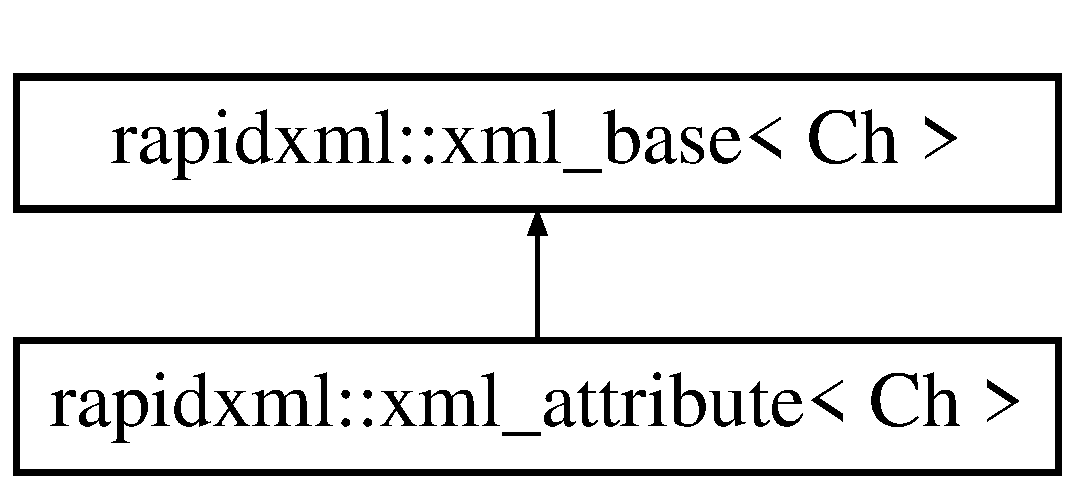
\includegraphics[height=2.000000cm]{classrapidxml_1_1xml__attribute}
\end{center}
\end{figure}
\subsection*{Public Member Functions}
\begin{DoxyCompactItemize}
\item 
\hyperlink{classrapidxml_1_1xml__attribute_a26be291103917d3e8de110d46dd83816}{xml\-\_\-attribute} ()
\item 
\hyperlink{classrapidxml_1_1xml__document}{xml\-\_\-document}$<$ Ch $>$ $\ast$ \hyperlink{classrapidxml_1_1xml__attribute_a8b6d31d899e27f01bde35b53d98496ec}{document} () const 
\item 
\hyperlink{classrapidxml_1_1xml__attribute}{xml\-\_\-attribute}$<$ Ch $>$ $\ast$ \hyperlink{classrapidxml_1_1xml__attribute_ae3547cc30b201fd6d7b98c04dda26f89}{previous\-\_\-attribute} (const Ch $\ast$\hyperlink{classrapidxml_1_1xml__base_a9a09739310469995db078ebd0da3ed45}{name}=0, std\-::size\-\_\-t \hyperlink{classrapidxml_1_1xml__base_a7e7f98b3d01e1eab8dc1ca69aad9af84}{name\-\_\-size}=0, bool case\-\_\-sensitive=true) const 
\item 
\hyperlink{classrapidxml_1_1xml__attribute}{xml\-\_\-attribute}$<$ Ch $>$ $\ast$ \hyperlink{classrapidxml_1_1xml__attribute_a56c08d7c96203286c889a43849328a86}{next\-\_\-attribute} (const Ch $\ast$\hyperlink{classrapidxml_1_1xml__base_a9a09739310469995db078ebd0da3ed45}{name}=0, std\-::size\-\_\-t \hyperlink{classrapidxml_1_1xml__base_a7e7f98b3d01e1eab8dc1ca69aad9af84}{name\-\_\-size}=0, bool case\-\_\-sensitive=true) const 
\end{DoxyCompactItemize}
\subsection*{Friends}
\begin{DoxyCompactItemize}
\item 
\hypertarget{classrapidxml_1_1xml__attribute_aa7e464ce3fe512598ff8dda47291941f}{class {\bfseries xml\-\_\-node$<$ Ch $>$}}\label{classrapidxml_1_1xml__attribute_aa7e464ce3fe512598ff8dda47291941f}

\end{DoxyCompactItemize}
\subsection*{Additional Inherited Members}


\subsection{Detailed Description}
\subsubsection*{template$<$class Ch$>$class rapidxml\-::xml\-\_\-attribute$<$ Ch $>$}

Class representing attribute node of X\-M\-L document. Each attribute has name and value strings, which are available through \hyperlink{classrapidxml_1_1xml__base_a9a09739310469995db078ebd0da3ed45}{name()} and \hyperlink{classrapidxml_1_1xml__base_adcdaccff61c665f039d9344e447b7445}{value()} functions (inherited from \hyperlink{classrapidxml_1_1xml__base}{xml\-\_\-base}). Note that after parse, both name and value of attribute will point to interior of source text used for parsing. Thus, this text must persist in memory for the lifetime of attribute. 
\begin{DoxyParams}{Parameters}
{\em Ch} & Character type to use. \\
\hline
\end{DoxyParams}


\subsection{Constructor \& Destructor Documentation}
\hypertarget{classrapidxml_1_1xml__attribute_a26be291103917d3e8de110d46dd83816}{\index{rapidxml\-::xml\-\_\-attribute@{rapidxml\-::xml\-\_\-attribute}!xml\-\_\-attribute@{xml\-\_\-attribute}}
\index{xml\-\_\-attribute@{xml\-\_\-attribute}!rapidxml::xml_attribute@{rapidxml\-::xml\-\_\-attribute}}
\subsubsection[{xml\-\_\-attribute}]{\setlength{\rightskip}{0pt plus 5cm}template$<$class Ch$>$ {\bf rapidxml\-::xml\-\_\-attribute}$<$ Ch $>$\-::{\bf xml\-\_\-attribute} (
\begin{DoxyParamCaption}
{}
\end{DoxyParamCaption}
)\hspace{0.3cm}{\ttfamily [inline]}}}\label{classrapidxml_1_1xml__attribute_a26be291103917d3e8de110d46dd83816}
Constructs an empty attribute with the specified type. Consider using \hyperlink{classrapidxml_1_1memory__pool}{memory\-\_\-pool} of appropriate \hyperlink{classrapidxml_1_1xml__document}{xml\-\_\-document} if allocating attributes manually. 

\subsection{Member Function Documentation}
\hypertarget{classrapidxml_1_1xml__attribute_a8b6d31d899e27f01bde35b53d98496ec}{\index{rapidxml\-::xml\-\_\-attribute@{rapidxml\-::xml\-\_\-attribute}!document@{document}}
\index{document@{document}!rapidxml::xml_attribute@{rapidxml\-::xml\-\_\-attribute}}
\subsubsection[{document}]{\setlength{\rightskip}{0pt plus 5cm}template$<$class Ch$>$ {\bf xml\-\_\-document}$<$Ch$>$$\ast$ {\bf rapidxml\-::xml\-\_\-attribute}$<$ Ch $>$\-::document (
\begin{DoxyParamCaption}
{}
\end{DoxyParamCaption}
) const\hspace{0.3cm}{\ttfamily [inline]}}}\label{classrapidxml_1_1xml__attribute_a8b6d31d899e27f01bde35b53d98496ec}
Gets document of which attribute is a child. \begin{DoxyReturn}{Returns}
Pointer to document that contains this attribute, or 0 if there is no parent document. 
\end{DoxyReturn}
\hypertarget{classrapidxml_1_1xml__attribute_a56c08d7c96203286c889a43849328a86}{\index{rapidxml\-::xml\-\_\-attribute@{rapidxml\-::xml\-\_\-attribute}!next\-\_\-attribute@{next\-\_\-attribute}}
\index{next\-\_\-attribute@{next\-\_\-attribute}!rapidxml::xml_attribute@{rapidxml\-::xml\-\_\-attribute}}
\subsubsection[{next\-\_\-attribute}]{\setlength{\rightskip}{0pt plus 5cm}template$<$class Ch$>$ {\bf xml\-\_\-attribute}$<$Ch$>$$\ast$ {\bf rapidxml\-::xml\-\_\-attribute}$<$ Ch $>$\-::next\-\_\-attribute (
\begin{DoxyParamCaption}
\item[{const Ch $\ast$}]{name = {\ttfamily 0}, }
\item[{std\-::size\-\_\-t}]{name\-\_\-size = {\ttfamily 0}, }
\item[{bool}]{case\-\_\-sensitive = {\ttfamily true}}
\end{DoxyParamCaption}
) const\hspace{0.3cm}{\ttfamily [inline]}}}\label{classrapidxml_1_1xml__attribute_a56c08d7c96203286c889a43849328a86}
Gets next attribute, optionally matching attribute name. 
\begin{DoxyParams}{Parameters}
{\em name} & Name of attribute to find, or 0 to return next attribute regardless of its name; this string doesn't have to be zero-\/terminated if name\-\_\-size is non-\/zero \\
\hline
{\em name\-\_\-size} & Size of name, in characters, or 0 to have size calculated automatically from string \\
\hline
{\em case\-\_\-sensitive} & Should name comparison be case-\/sensitive; non case-\/sensitive comparison works properly only for A\-S\-C\-I\-I characters \\
\hline
\end{DoxyParams}
\begin{DoxyReturn}{Returns}
Pointer to found attribute, or 0 if not found. 
\end{DoxyReturn}
\hypertarget{classrapidxml_1_1xml__attribute_ae3547cc30b201fd6d7b98c04dda26f89}{\index{rapidxml\-::xml\-\_\-attribute@{rapidxml\-::xml\-\_\-attribute}!previous\-\_\-attribute@{previous\-\_\-attribute}}
\index{previous\-\_\-attribute@{previous\-\_\-attribute}!rapidxml::xml_attribute@{rapidxml\-::xml\-\_\-attribute}}
\subsubsection[{previous\-\_\-attribute}]{\setlength{\rightskip}{0pt plus 5cm}template$<$class Ch$>$ {\bf xml\-\_\-attribute}$<$Ch$>$$\ast$ {\bf rapidxml\-::xml\-\_\-attribute}$<$ Ch $>$\-::previous\-\_\-attribute (
\begin{DoxyParamCaption}
\item[{const Ch $\ast$}]{name = {\ttfamily 0}, }
\item[{std\-::size\-\_\-t}]{name\-\_\-size = {\ttfamily 0}, }
\item[{bool}]{case\-\_\-sensitive = {\ttfamily true}}
\end{DoxyParamCaption}
) const\hspace{0.3cm}{\ttfamily [inline]}}}\label{classrapidxml_1_1xml__attribute_ae3547cc30b201fd6d7b98c04dda26f89}
Gets previous attribute, optionally matching attribute name. 
\begin{DoxyParams}{Parameters}
{\em name} & Name of attribute to find, or 0 to return previous attribute regardless of its name; this string doesn't have to be zero-\/terminated if name\-\_\-size is non-\/zero \\
\hline
{\em name\-\_\-size} & Size of name, in characters, or 0 to have size calculated automatically from string \\
\hline
{\em case\-\_\-sensitive} & Should name comparison be case-\/sensitive; non case-\/sensitive comparison works properly only for A\-S\-C\-I\-I characters \\
\hline
\end{DoxyParams}
\begin{DoxyReturn}{Returns}
Pointer to found attribute, or 0 if not found. 
\end{DoxyReturn}


The documentation for this class was generated from the following file\-:\begin{DoxyCompactItemize}
\item 
\hyperlink{rapidxml_8hpp}{rapidxml.\-hpp}\end{DoxyCompactItemize}

\hypertarget{classrapidxml_1_1xml__base}{\section{rapidxml\-:\-:xml\-\_\-base$<$ Ch $>$ Class Template Reference}
\label{classrapidxml_1_1xml__base}\index{rapidxml\-::xml\-\_\-base$<$ Ch $>$@{rapidxml\-::xml\-\_\-base$<$ Ch $>$}}
}


{\ttfamily \#include $<$rapidxml.\-hpp$>$}

Inheritance diagram for rapidxml\-:\-:xml\-\_\-base$<$ Ch $>$\-:\begin{figure}[H]
\begin{center}
\leavevmode
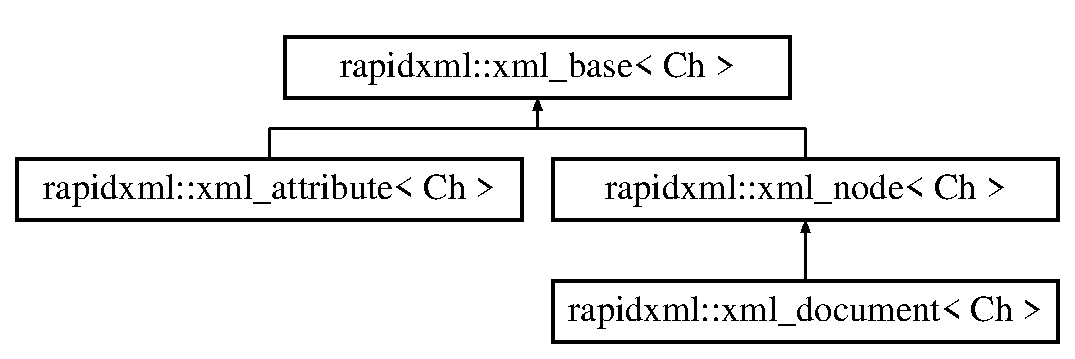
\includegraphics[height=3.000000cm]{classrapidxml_1_1xml__base}
\end{center}
\end{figure}
\subsection*{Public Member Functions}
\begin{DoxyCompactItemize}
\item 
Ch $\ast$ \hyperlink{classrapidxml_1_1xml__base_a9a09739310469995db078ebd0da3ed45}{name} () const 
\item 
std\-::size\-\_\-t \hyperlink{classrapidxml_1_1xml__base_a7e7f98b3d01e1eab8dc1ca69aad9af84}{name\-\_\-size} () const 
\item 
Ch $\ast$ \hyperlink{classrapidxml_1_1xml__base_adcdaccff61c665f039d9344e447b7445}{value} () const 
\item 
std\-::size\-\_\-t \hyperlink{classrapidxml_1_1xml__base_a9fcf201ed0915ac18dd43b0b5dcfaf32}{value\-\_\-size} () const 
\item 
void \hyperlink{classrapidxml_1_1xml__base_ae55060ae958c6e6465d6c8db852ec6ce}{name} (const Ch $\ast$name, std\-::size\-\_\-t size)
\item 
void \hyperlink{classrapidxml_1_1xml__base_a4611ddc82ac83a527c65606600eb2a0d}{name} (const Ch $\ast$name)
\item 
void \hyperlink{classrapidxml_1_1xml__base_a3b183c2db7022a6d30494dd2f0ac11e9}{value} (const Ch $\ast$value, std\-::size\-\_\-t size)
\item 
void \hyperlink{classrapidxml_1_1xml__base_a81e63ec4bfd2d7ef0a6c2ed49be6e623}{value} (const Ch $\ast$value)
\item 
\hyperlink{classrapidxml_1_1xml__node}{xml\-\_\-node}$<$ Ch $>$ $\ast$ \hyperlink{classrapidxml_1_1xml__base_a7f31ae930f93852830234db1ae59c4c4}{parent} () const 
\end{DoxyCompactItemize}
\subsection*{Static Protected Member Functions}
\begin{DoxyCompactItemize}
\item 
\hypertarget{classrapidxml_1_1xml__base_ad96ff6b1e41dab3ff60b9bc4df769a75}{static Ch $\ast$ {\bfseries nullstr} ()}\label{classrapidxml_1_1xml__base_ad96ff6b1e41dab3ff60b9bc4df769a75}

\end{DoxyCompactItemize}
\subsection*{Protected Attributes}
\begin{DoxyCompactItemize}
\item 
\hypertarget{classrapidxml_1_1xml__base_afd9851ed43e14619db0d7075ef8e9e8a}{Ch $\ast$ {\bfseries m\-\_\-name}}\label{classrapidxml_1_1xml__base_afd9851ed43e14619db0d7075ef8e9e8a}

\item 
\hypertarget{classrapidxml_1_1xml__base_a278a1ea63b0b70219b946cec47fa00ea}{Ch $\ast$ {\bfseries m\-\_\-value}}\label{classrapidxml_1_1xml__base_a278a1ea63b0b70219b946cec47fa00ea}

\item 
\hypertarget{classrapidxml_1_1xml__base_a5a8c76a7274b4180213796422c4df76f}{std\-::size\-\_\-t {\bfseries m\-\_\-name\-\_\-size}}\label{classrapidxml_1_1xml__base_a5a8c76a7274b4180213796422c4df76f}

\item 
\hypertarget{classrapidxml_1_1xml__base_aa3a49d8ceddb8a8d7edb773a2226b89c}{std\-::size\-\_\-t {\bfseries m\-\_\-value\-\_\-size}}\label{classrapidxml_1_1xml__base_aa3a49d8ceddb8a8d7edb773a2226b89c}

\item 
\hypertarget{classrapidxml_1_1xml__base_a90d5f660f078f66563fd7b2d8387ccb0}{\hyperlink{classrapidxml_1_1xml__node}{xml\-\_\-node}$<$ Ch $>$ $\ast$ {\bfseries m\-\_\-parent}}\label{classrapidxml_1_1xml__base_a90d5f660f078f66563fd7b2d8387ccb0}

\end{DoxyCompactItemize}


\subsection{Detailed Description}
\subsubsection*{template$<$class Ch = char$>$class rapidxml\-::xml\-\_\-base$<$ Ch $>$}

Base class for \hyperlink{classrapidxml_1_1xml__node}{xml\-\_\-node} and \hyperlink{classrapidxml_1_1xml__attribute}{xml\-\_\-attribute} implementing common functions\-: \hyperlink{classrapidxml_1_1xml__base_a9a09739310469995db078ebd0da3ed45}{name()}, \hyperlink{classrapidxml_1_1xml__base_a7e7f98b3d01e1eab8dc1ca69aad9af84}{name\-\_\-size()}, \hyperlink{classrapidxml_1_1xml__base_adcdaccff61c665f039d9344e447b7445}{value()}, \hyperlink{classrapidxml_1_1xml__base_a9fcf201ed0915ac18dd43b0b5dcfaf32}{value\-\_\-size()} and \hyperlink{classrapidxml_1_1xml__base_a7f31ae930f93852830234db1ae59c4c4}{parent()}. 
\begin{DoxyParams}{Parameters}
{\em Ch} & Character type to use \\
\hline
\end{DoxyParams}


\subsection{Member Function Documentation}
\hypertarget{classrapidxml_1_1xml__base_a9a09739310469995db078ebd0da3ed45}{\index{rapidxml\-::xml\-\_\-base@{rapidxml\-::xml\-\_\-base}!name@{name}}
\index{name@{name}!rapidxml::xml_base@{rapidxml\-::xml\-\_\-base}}
\subsubsection[{name}]{\setlength{\rightskip}{0pt plus 5cm}template$<$class Ch  = char$>$ Ch$\ast$ {\bf rapidxml\-::xml\-\_\-base}$<$ Ch $>$\-::name (
\begin{DoxyParamCaption}
{}
\end{DoxyParamCaption}
) const\hspace{0.3cm}{\ttfamily [inline]}}}\label{classrapidxml_1_1xml__base_a9a09739310469995db078ebd0da3ed45}
Gets name of the node. Interpretation of name depends on type of node. Note that name will not be zero-\/terminated if rapidxml\-::parse\-\_\-no\-\_\-string\-\_\-terminators option was selected during parse. \par
\par
 Use \hyperlink{classrapidxml_1_1xml__base_a7e7f98b3d01e1eab8dc1ca69aad9af84}{name\-\_\-size()} function to determine length of the name. \begin{DoxyReturn}{Returns}
Name of node, or empty string if node has no name. 
\end{DoxyReturn}
\hypertarget{classrapidxml_1_1xml__base_ae55060ae958c6e6465d6c8db852ec6ce}{\index{rapidxml\-::xml\-\_\-base@{rapidxml\-::xml\-\_\-base}!name@{name}}
\index{name@{name}!rapidxml::xml_base@{rapidxml\-::xml\-\_\-base}}
\subsubsection[{name}]{\setlength{\rightskip}{0pt plus 5cm}template$<$class Ch  = char$>$ void {\bf rapidxml\-::xml\-\_\-base}$<$ Ch $>$\-::name (
\begin{DoxyParamCaption}
\item[{const Ch $\ast$}]{name, }
\item[{std\-::size\-\_\-t}]{size}
\end{DoxyParamCaption}
)\hspace{0.3cm}{\ttfamily [inline]}}}\label{classrapidxml_1_1xml__base_ae55060ae958c6e6465d6c8db852ec6ce}
Sets name of node to a non zero-\/terminated string. See ownership\-\_\-of\-\_\-strings. \par
\par
 Note that node does not own its name or value, it only stores a pointer to it. It will not delete or otherwise free the pointer on destruction. It is reponsibility of the user to properly manage lifetime of the string. The easiest way to achieve it is to use \hyperlink{classrapidxml_1_1memory__pool}{memory\-\_\-pool} of the document to allocate the string -\/ on destruction of the document the string will be automatically freed. \par
\par
 Size of name must be specified separately, because name does not have to be zero terminated. Use \hyperlink{classrapidxml_1_1xml__base_a4611ddc82ac83a527c65606600eb2a0d}{name(const Ch $\ast$)} function to have the length automatically calculated (string must be zero terminated). 
\begin{DoxyParams}{Parameters}
{\em name} & Name of node to set. Does not have to be zero terminated. \\
\hline
{\em size} & Size of name, in characters. This does not include zero terminator, if one is present. \\
\hline
\end{DoxyParams}
\hypertarget{classrapidxml_1_1xml__base_a4611ddc82ac83a527c65606600eb2a0d}{\index{rapidxml\-::xml\-\_\-base@{rapidxml\-::xml\-\_\-base}!name@{name}}
\index{name@{name}!rapidxml::xml_base@{rapidxml\-::xml\-\_\-base}}
\subsubsection[{name}]{\setlength{\rightskip}{0pt plus 5cm}template$<$class Ch  = char$>$ void {\bf rapidxml\-::xml\-\_\-base}$<$ Ch $>$\-::name (
\begin{DoxyParamCaption}
\item[{const Ch $\ast$}]{name}
\end{DoxyParamCaption}
)\hspace{0.3cm}{\ttfamily [inline]}}}\label{classrapidxml_1_1xml__base_a4611ddc82ac83a527c65606600eb2a0d}
Sets name of node to a zero-\/terminated string. See also ownership\-\_\-of\-\_\-strings and \hyperlink{classrapidxml_1_1xml__base_ae55060ae958c6e6465d6c8db852ec6ce}{xml\-\_\-node\-::name(const Ch $\ast$, std\-::size\-\_\-t)}. 
\begin{DoxyParams}{Parameters}
{\em name} & Name of node to set. Must be zero terminated. \\
\hline
\end{DoxyParams}
\hypertarget{classrapidxml_1_1xml__base_a7e7f98b3d01e1eab8dc1ca69aad9af84}{\index{rapidxml\-::xml\-\_\-base@{rapidxml\-::xml\-\_\-base}!name\-\_\-size@{name\-\_\-size}}
\index{name\-\_\-size@{name\-\_\-size}!rapidxml::xml_base@{rapidxml\-::xml\-\_\-base}}
\subsubsection[{name\-\_\-size}]{\setlength{\rightskip}{0pt plus 5cm}template$<$class Ch  = char$>$ std\-::size\-\_\-t {\bf rapidxml\-::xml\-\_\-base}$<$ Ch $>$\-::name\-\_\-size (
\begin{DoxyParamCaption}
{}
\end{DoxyParamCaption}
) const\hspace{0.3cm}{\ttfamily [inline]}}}\label{classrapidxml_1_1xml__base_a7e7f98b3d01e1eab8dc1ca69aad9af84}
Gets size of node name, not including terminator character. This function works correctly irrespective of whether name is or is not zero terminated. \begin{DoxyReturn}{Returns}
Size of node name, in characters. 
\end{DoxyReturn}
\hypertarget{classrapidxml_1_1xml__base_a7f31ae930f93852830234db1ae59c4c4}{\index{rapidxml\-::xml\-\_\-base@{rapidxml\-::xml\-\_\-base}!parent@{parent}}
\index{parent@{parent}!rapidxml::xml_base@{rapidxml\-::xml\-\_\-base}}
\subsubsection[{parent}]{\setlength{\rightskip}{0pt plus 5cm}template$<$class Ch  = char$>$ {\bf xml\-\_\-node}$<$Ch$>$$\ast$ {\bf rapidxml\-::xml\-\_\-base}$<$ Ch $>$\-::parent (
\begin{DoxyParamCaption}
{}
\end{DoxyParamCaption}
) const\hspace{0.3cm}{\ttfamily [inline]}}}\label{classrapidxml_1_1xml__base_a7f31ae930f93852830234db1ae59c4c4}
Gets node parent. \begin{DoxyReturn}{Returns}
Pointer to parent node, or 0 if there is no parent. 
\end{DoxyReturn}
\hypertarget{classrapidxml_1_1xml__base_adcdaccff61c665f039d9344e447b7445}{\index{rapidxml\-::xml\-\_\-base@{rapidxml\-::xml\-\_\-base}!value@{value}}
\index{value@{value}!rapidxml::xml_base@{rapidxml\-::xml\-\_\-base}}
\subsubsection[{value}]{\setlength{\rightskip}{0pt plus 5cm}template$<$class Ch  = char$>$ Ch$\ast$ {\bf rapidxml\-::xml\-\_\-base}$<$ Ch $>$\-::value (
\begin{DoxyParamCaption}
{}
\end{DoxyParamCaption}
) const\hspace{0.3cm}{\ttfamily [inline]}}}\label{classrapidxml_1_1xml__base_adcdaccff61c665f039d9344e447b7445}
Gets value of node. Interpretation of value depends on type of node. Note that value will not be zero-\/terminated if rapidxml\-::parse\-\_\-no\-\_\-string\-\_\-terminators option was selected during parse. \par
\par
 Use \hyperlink{classrapidxml_1_1xml__base_a9fcf201ed0915ac18dd43b0b5dcfaf32}{value\-\_\-size()} function to determine length of the value. \begin{DoxyReturn}{Returns}
Value of node, or empty string if node has no value. 
\end{DoxyReturn}
\hypertarget{classrapidxml_1_1xml__base_a3b183c2db7022a6d30494dd2f0ac11e9}{\index{rapidxml\-::xml\-\_\-base@{rapidxml\-::xml\-\_\-base}!value@{value}}
\index{value@{value}!rapidxml::xml_base@{rapidxml\-::xml\-\_\-base}}
\subsubsection[{value}]{\setlength{\rightskip}{0pt plus 5cm}template$<$class Ch  = char$>$ void {\bf rapidxml\-::xml\-\_\-base}$<$ Ch $>$\-::value (
\begin{DoxyParamCaption}
\item[{const Ch $\ast$}]{value, }
\item[{std\-::size\-\_\-t}]{size}
\end{DoxyParamCaption}
)\hspace{0.3cm}{\ttfamily [inline]}}}\label{classrapidxml_1_1xml__base_a3b183c2db7022a6d30494dd2f0ac11e9}
Sets value of node to a non zero-\/terminated string. See ownership\-\_\-of\-\_\-strings. \par
\par
 Note that node does not own its name or value, it only stores a pointer to it. It will not delete or otherwise free the pointer on destruction. It is reponsibility of the user to properly manage lifetime of the string. The easiest way to achieve it is to use \hyperlink{classrapidxml_1_1memory__pool}{memory\-\_\-pool} of the document to allocate the string -\/ on destruction of the document the string will be automatically freed. \par
\par
 Size of value must be specified separately, because it does not have to be zero terminated. Use \hyperlink{classrapidxml_1_1xml__base_a81e63ec4bfd2d7ef0a6c2ed49be6e623}{value(const Ch $\ast$)} function to have the length automatically calculated (string must be zero terminated). \par
\par
 If an element has a child node of type node\-\_\-data, it will take precedence over element value when printing. If you want to manipulate data of elements using values, use parser flag rapidxml\-::parse\-\_\-no\-\_\-data\-\_\-nodes to prevent creation of data nodes by the parser. 
\begin{DoxyParams}{Parameters}
{\em value} & value of node to set. Does not have to be zero terminated. \\
\hline
{\em size} & Size of value, in characters. This does not include zero terminator, if one is present. \\
\hline
\end{DoxyParams}
\hypertarget{classrapidxml_1_1xml__base_a81e63ec4bfd2d7ef0a6c2ed49be6e623}{\index{rapidxml\-::xml\-\_\-base@{rapidxml\-::xml\-\_\-base}!value@{value}}
\index{value@{value}!rapidxml::xml_base@{rapidxml\-::xml\-\_\-base}}
\subsubsection[{value}]{\setlength{\rightskip}{0pt plus 5cm}template$<$class Ch  = char$>$ void {\bf rapidxml\-::xml\-\_\-base}$<$ Ch $>$\-::value (
\begin{DoxyParamCaption}
\item[{const Ch $\ast$}]{value}
\end{DoxyParamCaption}
)\hspace{0.3cm}{\ttfamily [inline]}}}\label{classrapidxml_1_1xml__base_a81e63ec4bfd2d7ef0a6c2ed49be6e623}
Sets value of node to a zero-\/terminated string. See also ownership\-\_\-of\-\_\-strings and \hyperlink{classrapidxml_1_1xml__base_a3b183c2db7022a6d30494dd2f0ac11e9}{xml\-\_\-node\-::value(const Ch $\ast$, std\-::size\-\_\-t)}. 
\begin{DoxyParams}{Parameters}
{\em value} & Vame of node to set. Must be zero terminated. \\
\hline
\end{DoxyParams}
\hypertarget{classrapidxml_1_1xml__base_a9fcf201ed0915ac18dd43b0b5dcfaf32}{\index{rapidxml\-::xml\-\_\-base@{rapidxml\-::xml\-\_\-base}!value\-\_\-size@{value\-\_\-size}}
\index{value\-\_\-size@{value\-\_\-size}!rapidxml::xml_base@{rapidxml\-::xml\-\_\-base}}
\subsubsection[{value\-\_\-size}]{\setlength{\rightskip}{0pt plus 5cm}template$<$class Ch  = char$>$ std\-::size\-\_\-t {\bf rapidxml\-::xml\-\_\-base}$<$ Ch $>$\-::value\-\_\-size (
\begin{DoxyParamCaption}
{}
\end{DoxyParamCaption}
) const\hspace{0.3cm}{\ttfamily [inline]}}}\label{classrapidxml_1_1xml__base_a9fcf201ed0915ac18dd43b0b5dcfaf32}
Gets size of node value, not including terminator character. This function works correctly irrespective of whether value is or is not zero terminated. \begin{DoxyReturn}{Returns}
Size of node value, in characters. 
\end{DoxyReturn}


The documentation for this class was generated from the following file\-:\begin{DoxyCompactItemize}
\item 
\hyperlink{rapidxml_8hpp}{rapidxml.\-hpp}\end{DoxyCompactItemize}

\hypertarget{classrapidxml_1_1xml__document}{\section{rapidxml\-:\-:xml\-\_\-document$<$ Ch $>$ Class Template Reference}
\label{classrapidxml_1_1xml__document}\index{rapidxml\-::xml\-\_\-document$<$ Ch $>$@{rapidxml\-::xml\-\_\-document$<$ Ch $>$}}
}


{\ttfamily \#include $<$rapidxml.\-hpp$>$}

Inheritance diagram for rapidxml\-:\-:xml\-\_\-document$<$ Ch $>$\-:\begin{figure}[H]
\begin{center}
\leavevmode
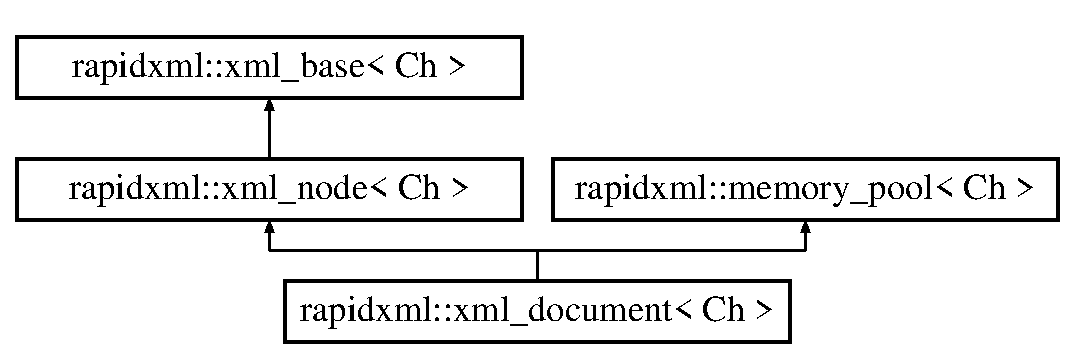
\includegraphics[height=3.000000cm]{classrapidxml_1_1xml__document}
\end{center}
\end{figure}
\subsection*{Public Member Functions}
\begin{DoxyCompactItemize}
\item 
\hypertarget{classrapidxml_1_1xml__document_aae8841b15085ba8f32ff46587ace28f5}{\hyperlink{classrapidxml_1_1xml__document_aae8841b15085ba8f32ff46587ace28f5}{xml\-\_\-document} ()}\label{classrapidxml_1_1xml__document_aae8841b15085ba8f32ff46587ace28f5}

\begin{DoxyCompactList}\small\item\em Constructs empty X\-M\-L document. \end{DoxyCompactList}\item 
{\footnotesize template$<$int Flags$>$ }\\void \hyperlink{classrapidxml_1_1xml__document_ac6e73ff9ac323bf5a370c38feb03a6b1}{parse} (Ch $\ast$text)
\item 
void \hyperlink{classrapidxml_1_1xml__document_a826929ff54242532198701f19ff5f83f}{clear} ()
\end{DoxyCompactItemize}
\subsection*{Additional Inherited Members}


\subsection{Detailed Description}
\subsubsection*{template$<$class Ch$>$class rapidxml\-::xml\-\_\-document$<$ Ch $>$}

This class represents root of the D\-O\-M hierarchy. It is also an \hyperlink{classrapidxml_1_1xml__node}{xml\-\_\-node} and a \hyperlink{classrapidxml_1_1memory__pool}{memory\-\_\-pool} through public inheritance. Use \hyperlink{classrapidxml_1_1xml__document_ac6e73ff9ac323bf5a370c38feb03a6b1}{parse()} function to build a D\-O\-M tree from a zero-\/terminated X\-M\-L text string. \hyperlink{classrapidxml_1_1xml__document_ac6e73ff9ac323bf5a370c38feb03a6b1}{parse()} function allocates memory for nodes and attributes by using functions of \hyperlink{classrapidxml_1_1xml__document}{xml\-\_\-document}, which are inherited from \hyperlink{classrapidxml_1_1memory__pool}{memory\-\_\-pool}. To access root node of the document, use the document itself, as if it was an \hyperlink{classrapidxml_1_1xml__node}{xml\-\_\-node}. 
\begin{DoxyParams}{Parameters}
{\em Ch} & Character type to use. \\
\hline
\end{DoxyParams}


\subsection{Member Function Documentation}
\hypertarget{classrapidxml_1_1xml__document_a826929ff54242532198701f19ff5f83f}{\index{rapidxml\-::xml\-\_\-document@{rapidxml\-::xml\-\_\-document}!clear@{clear}}
\index{clear@{clear}!rapidxml::xml_document@{rapidxml\-::xml\-\_\-document}}
\subsubsection[{clear}]{\setlength{\rightskip}{0pt plus 5cm}template$<$class Ch $>$ void {\bf rapidxml\-::xml\-\_\-document}$<$ Ch $>$\-::clear (
\begin{DoxyParamCaption}
{}
\end{DoxyParamCaption}
)\hspace{0.3cm}{\ttfamily [inline]}}}\label{classrapidxml_1_1xml__document_a826929ff54242532198701f19ff5f83f}
Clears the document by deleting all nodes and clearing the memory pool. All nodes owned by document pool are destroyed. \hypertarget{classrapidxml_1_1xml__document_ac6e73ff9ac323bf5a370c38feb03a6b1}{\index{rapidxml\-::xml\-\_\-document@{rapidxml\-::xml\-\_\-document}!parse@{parse}}
\index{parse@{parse}!rapidxml::xml_document@{rapidxml\-::xml\-\_\-document}}
\subsubsection[{parse}]{\setlength{\rightskip}{0pt plus 5cm}template$<$class Ch $>$ template$<$int Flags$>$ void {\bf rapidxml\-::xml\-\_\-document}$<$ Ch $>$\-::parse (
\begin{DoxyParamCaption}
\item[{Ch $\ast$}]{text}
\end{DoxyParamCaption}
)\hspace{0.3cm}{\ttfamily [inline]}}}\label{classrapidxml_1_1xml__document_ac6e73ff9ac323bf5a370c38feb03a6b1}
Parses zero-\/terminated X\-M\-L string according to given flags. Passed string will be modified by the parser, unless rapidxml\-::parse\-\_\-non\-\_\-destructive flag is used. The string must persist for the lifetime of the document. In case of error, \hyperlink{classrapidxml_1_1parse__error}{rapidxml\-::parse\-\_\-error} exception will be thrown. \par
\par
 If you want to parse contents of a file, you must first load the file into the memory, and pass pointer to its beginning. Make sure that data is zero-\/terminated. \par
\par
 Document can be parsed into multiple times. Each new call to parse removes previous nodes and attributes (if any), but does not clear memory pool. 
\begin{DoxyParams}{Parameters}
{\em text} & X\-M\-L data to parse; pointer is non-\/const to denote fact that this data may be modified by the parser. \\
\hline
\end{DoxyParams}


The documentation for this class was generated from the following file\-:\begin{DoxyCompactItemize}
\item 
\hyperlink{rapidxml_8hpp}{rapidxml.\-hpp}\end{DoxyCompactItemize}

\hypertarget{classrapidxml_1_1xml__node}{\section{rapidxml\-:\-:xml\-\_\-node$<$ Ch $>$ Class Template Reference}
\label{classrapidxml_1_1xml__node}\index{rapidxml\-::xml\-\_\-node$<$ Ch $>$@{rapidxml\-::xml\-\_\-node$<$ Ch $>$}}
}


{\ttfamily \#include $<$rapidxml.\-hpp$>$}

Inheritance diagram for rapidxml\-:\-:xml\-\_\-node$<$ Ch $>$\-:\begin{figure}[H]
\begin{center}
\leavevmode
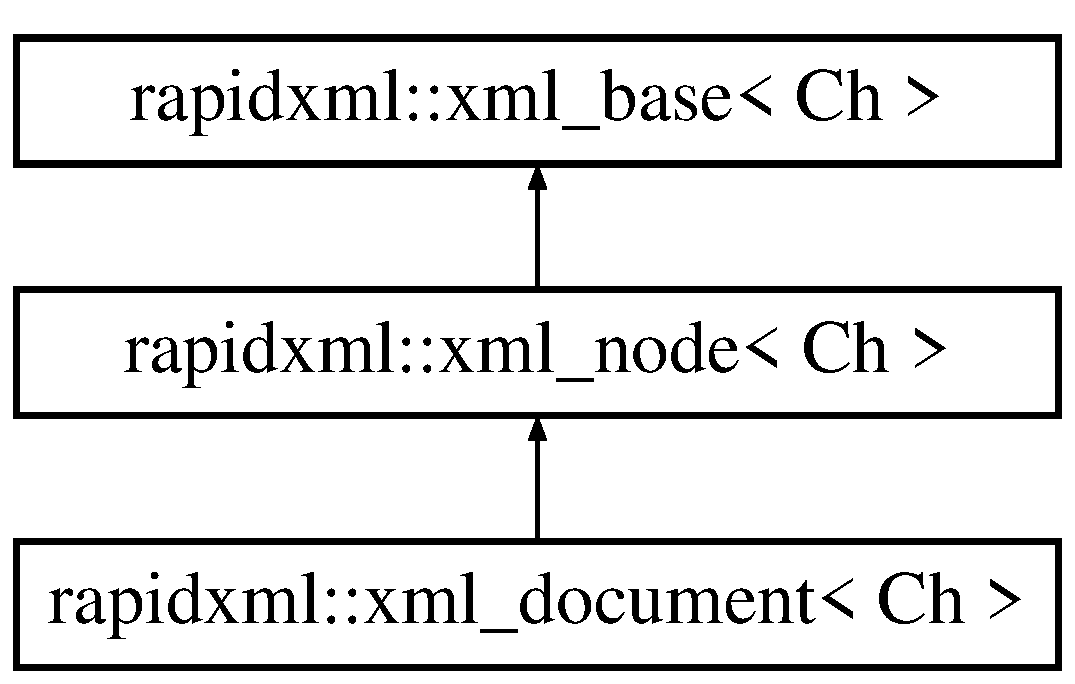
\includegraphics[height=3.000000cm]{classrapidxml_1_1xml__node}
\end{center}
\end{figure}
\subsection*{Public Member Functions}
\begin{DoxyCompactItemize}
\item 
\hyperlink{classrapidxml_1_1xml__node_a8bd9019960b90605a45998b661fb1b0e}{xml\-\_\-node} (node\-\_\-type \hyperlink{classrapidxml_1_1xml__node_a2c6a4315b98bcfa2e04fed3fa1b22c36}{type})
\item 
node\-\_\-type \hyperlink{classrapidxml_1_1xml__node_a2c6a4315b98bcfa2e04fed3fa1b22c36}{type} () const 
\item 
\hyperlink{classrapidxml_1_1xml__document}{xml\-\_\-document}$<$ Ch $>$ $\ast$ \hyperlink{classrapidxml_1_1xml__node_adb6ad21a4590cf13d4a6a5036e3cdbbc}{document} () const 
\item 
\hyperlink{classrapidxml_1_1xml__node}{xml\-\_\-node}$<$ Ch $>$ $\ast$ \hyperlink{classrapidxml_1_1xml__node_a2dedeb4e04bb35e06a9a7bddf6ba652d}{first\-\_\-node} (const Ch $\ast$\hyperlink{classrapidxml_1_1xml__base_a9a09739310469995db078ebd0da3ed45}{name}=0, std\-::size\-\_\-t \hyperlink{classrapidxml_1_1xml__base_a7e7f98b3d01e1eab8dc1ca69aad9af84}{name\-\_\-size}=0, bool case\-\_\-sensitive=true) const 
\item 
\hyperlink{classrapidxml_1_1xml__node}{xml\-\_\-node}$<$ Ch $>$ $\ast$ \hyperlink{classrapidxml_1_1xml__node_a2ace550c18cf10da6303773972d7157f}{last\-\_\-node} (const Ch $\ast$\hyperlink{classrapidxml_1_1xml__base_a9a09739310469995db078ebd0da3ed45}{name}=0, std\-::size\-\_\-t \hyperlink{classrapidxml_1_1xml__base_a7e7f98b3d01e1eab8dc1ca69aad9af84}{name\-\_\-size}=0, bool case\-\_\-sensitive=true) const 
\item 
\hyperlink{classrapidxml_1_1xml__node}{xml\-\_\-node}$<$ Ch $>$ $\ast$ \hyperlink{classrapidxml_1_1xml__node_a001ece4e227eebbd6ad0ec7dacf1c00b}{previous\-\_\-sibling} (const Ch $\ast$\hyperlink{classrapidxml_1_1xml__base_a9a09739310469995db078ebd0da3ed45}{name}=0, std\-::size\-\_\-t \hyperlink{classrapidxml_1_1xml__base_a7e7f98b3d01e1eab8dc1ca69aad9af84}{name\-\_\-size}=0, bool case\-\_\-sensitive=true) const 
\item 
\hyperlink{classrapidxml_1_1xml__node}{xml\-\_\-node}$<$ Ch $>$ $\ast$ \hyperlink{classrapidxml_1_1xml__node_ac59af4dd5f0ec715753e42467dff6aed}{next\-\_\-sibling} (const Ch $\ast$\hyperlink{classrapidxml_1_1xml__base_a9a09739310469995db078ebd0da3ed45}{name}=0, std\-::size\-\_\-t \hyperlink{classrapidxml_1_1xml__base_a7e7f98b3d01e1eab8dc1ca69aad9af84}{name\-\_\-size}=0, bool case\-\_\-sensitive=true) const 
\item 
\hyperlink{classrapidxml_1_1xml__attribute}{xml\-\_\-attribute}$<$ Ch $>$ $\ast$ \hyperlink{classrapidxml_1_1xml__node_ae426802be58114ffc41bf30ac6b8c37d}{first\-\_\-attribute} (const Ch $\ast$\hyperlink{classrapidxml_1_1xml__base_a9a09739310469995db078ebd0da3ed45}{name}=0, std\-::size\-\_\-t \hyperlink{classrapidxml_1_1xml__base_a7e7f98b3d01e1eab8dc1ca69aad9af84}{name\-\_\-size}=0, bool case\-\_\-sensitive=true) const 
\item 
\hyperlink{classrapidxml_1_1xml__attribute}{xml\-\_\-attribute}$<$ Ch $>$ $\ast$ \hyperlink{classrapidxml_1_1xml__node_a50c03f2db3fa51f27a73d86ec29a49d3}{last\-\_\-attribute} (const Ch $\ast$\hyperlink{classrapidxml_1_1xml__base_a9a09739310469995db078ebd0da3ed45}{name}=0, std\-::size\-\_\-t \hyperlink{classrapidxml_1_1xml__base_a7e7f98b3d01e1eab8dc1ca69aad9af84}{name\-\_\-size}=0, bool case\-\_\-sensitive=true) const 
\item 
void \hyperlink{classrapidxml_1_1xml__node_a499bbc9300c1b06821d5c08b24164c68}{type} (node\-\_\-type type)
\item 
void \hyperlink{classrapidxml_1_1xml__node_ae86e92908c3eab40bbed8216e4f3f3cb}{prepend\-\_\-node} (\hyperlink{classrapidxml_1_1xml__node}{xml\-\_\-node}$<$ Ch $>$ $\ast$child)
\item 
void \hyperlink{classrapidxml_1_1xml__node_a8696d098ecc9c4d2a646b43e91d58e31}{append\-\_\-node} (\hyperlink{classrapidxml_1_1xml__node}{xml\-\_\-node}$<$ Ch $>$ $\ast$child)
\item 
void \hyperlink{classrapidxml_1_1xml__node_a666880f42a7e486d78cc45ed51c7c46d}{insert\-\_\-node} (\hyperlink{classrapidxml_1_1xml__node}{xml\-\_\-node}$<$ Ch $>$ $\ast$where, \hyperlink{classrapidxml_1_1xml__node}{xml\-\_\-node}$<$ Ch $>$ $\ast$child)
\item 
void \hyperlink{classrapidxml_1_1xml__node_a62bf7b276cf7a651a3337f5e0a0ef6ac}{remove\-\_\-first\-\_\-node} ()
\item 
void \hyperlink{classrapidxml_1_1xml__node_a9182512e948ec451a83f116cce7c7674}{remove\-\_\-last\-\_\-node} ()
\item 
\hypertarget{classrapidxml_1_1xml__node_a98289923eb9e8889418a9eb0207ea35c}{void \hyperlink{classrapidxml_1_1xml__node_a98289923eb9e8889418a9eb0207ea35c}{remove\-\_\-node} (\hyperlink{classrapidxml_1_1xml__node}{xml\-\_\-node}$<$ Ch $>$ $\ast$where)}\label{classrapidxml_1_1xml__node_a98289923eb9e8889418a9eb0207ea35c}

\begin{DoxyCompactList}\small\item\em Removes specified child from the node. \end{DoxyCompactList}\item 
\hypertarget{classrapidxml_1_1xml__node_a95735358b079ae0adcfbbac69aa1fbc3}{void \hyperlink{classrapidxml_1_1xml__node_a95735358b079ae0adcfbbac69aa1fbc3}{remove\-\_\-all\-\_\-nodes} ()}\label{classrapidxml_1_1xml__node_a95735358b079ae0adcfbbac69aa1fbc3}

\begin{DoxyCompactList}\small\item\em Removes all child nodes (but not attributes). \end{DoxyCompactList}\item 
void \hyperlink{classrapidxml_1_1xml__node_a8b62ee76489faf8e2d1210869d547684}{prepend\-\_\-attribute} (\hyperlink{classrapidxml_1_1xml__attribute}{xml\-\_\-attribute}$<$ Ch $>$ $\ast$attribute)
\item 
void \hyperlink{classrapidxml_1_1xml__node_a33ce3386f8c42dd4db658b75cbb6e6c4}{append\-\_\-attribute} (\hyperlink{classrapidxml_1_1xml__attribute}{xml\-\_\-attribute}$<$ Ch $>$ $\ast$attribute)
\item 
void \hyperlink{classrapidxml_1_1xml__node_a9fe659cdf4a5b3bbf5e8ffc98db5a84f}{insert\-\_\-attribute} (\hyperlink{classrapidxml_1_1xml__attribute}{xml\-\_\-attribute}$<$ Ch $>$ $\ast$where, \hyperlink{classrapidxml_1_1xml__attribute}{xml\-\_\-attribute}$<$ Ch $>$ $\ast$attribute)
\item 
void \hyperlink{classrapidxml_1_1xml__node_aa95192d2a165cca16c551ed2a2a06aec}{remove\-\_\-first\-\_\-attribute} ()
\item 
void \hyperlink{classrapidxml_1_1xml__node_a1781a2cbedc9a51d609ad5b528125635}{remove\-\_\-last\-\_\-attribute} ()
\item 
void \hyperlink{classrapidxml_1_1xml__node_a6f97b1b4f46a94a4587915df3c0c6b57}{remove\-\_\-attribute} (\hyperlink{classrapidxml_1_1xml__attribute}{xml\-\_\-attribute}$<$ Ch $>$ $\ast$where)
\item 
\hypertarget{classrapidxml_1_1xml__node_aa8d5d9484aa1eb5ff1841a073c84c1aa}{void \hyperlink{classrapidxml_1_1xml__node_aa8d5d9484aa1eb5ff1841a073c84c1aa}{remove\-\_\-all\-\_\-attributes} ()}\label{classrapidxml_1_1xml__node_aa8d5d9484aa1eb5ff1841a073c84c1aa}

\begin{DoxyCompactList}\small\item\em Removes all attributes of node. \end{DoxyCompactList}\end{DoxyCompactItemize}
\subsection*{Additional Inherited Members}


\subsection{Detailed Description}
\subsubsection*{template$<$class Ch$>$class rapidxml\-::xml\-\_\-node$<$ Ch $>$}

Class representing a node of X\-M\-L document. Each node may have associated name and value strings, which are available through \hyperlink{classrapidxml_1_1xml__base_a9a09739310469995db078ebd0da3ed45}{name()} and \hyperlink{classrapidxml_1_1xml__base_adcdaccff61c665f039d9344e447b7445}{value()} functions. Interpretation of name and value depends on type of the node. Type of node can be determined by using \hyperlink{classrapidxml_1_1xml__node_a2c6a4315b98bcfa2e04fed3fa1b22c36}{type()} function. \par
\par
 Note that after parse, both name and value of node, if any, will point interior of source text used for parsing. Thus, this text must persist in the memory for the lifetime of node. 
\begin{DoxyParams}{Parameters}
{\em Ch} & Character type to use. \\
\hline
\end{DoxyParams}


\subsection{Constructor \& Destructor Documentation}
\hypertarget{classrapidxml_1_1xml__node_a8bd9019960b90605a45998b661fb1b0e}{\index{rapidxml\-::xml\-\_\-node@{rapidxml\-::xml\-\_\-node}!xml\-\_\-node@{xml\-\_\-node}}
\index{xml\-\_\-node@{xml\-\_\-node}!rapidxml::xml_node@{rapidxml\-::xml\-\_\-node}}
\subsubsection[{xml\-\_\-node}]{\setlength{\rightskip}{0pt plus 5cm}template$<$class Ch$>$ {\bf rapidxml\-::xml\-\_\-node}$<$ Ch $>$\-::{\bf xml\-\_\-node} (
\begin{DoxyParamCaption}
\item[{node\-\_\-type}]{type}
\end{DoxyParamCaption}
)\hspace{0.3cm}{\ttfamily [inline]}}}\label{classrapidxml_1_1xml__node_a8bd9019960b90605a45998b661fb1b0e}
Constructs an empty node with the specified type. Consider using \hyperlink{classrapidxml_1_1memory__pool}{memory\-\_\-pool} of appropriate document to allocate nodes manually. 
\begin{DoxyParams}{Parameters}
{\em type} & Type of node to construct. \\
\hline
\end{DoxyParams}


\subsection{Member Function Documentation}
\hypertarget{classrapidxml_1_1xml__node_a33ce3386f8c42dd4db658b75cbb6e6c4}{\index{rapidxml\-::xml\-\_\-node@{rapidxml\-::xml\-\_\-node}!append\-\_\-attribute@{append\-\_\-attribute}}
\index{append\-\_\-attribute@{append\-\_\-attribute}!rapidxml::xml_node@{rapidxml\-::xml\-\_\-node}}
\subsubsection[{append\-\_\-attribute}]{\setlength{\rightskip}{0pt plus 5cm}template$<$class Ch$>$ void {\bf rapidxml\-::xml\-\_\-node}$<$ Ch $>$\-::append\-\_\-attribute (
\begin{DoxyParamCaption}
\item[{{\bf xml\-\_\-attribute}$<$ Ch $>$ $\ast$}]{attribute}
\end{DoxyParamCaption}
)\hspace{0.3cm}{\ttfamily [inline]}}}\label{classrapidxml_1_1xml__node_a33ce3386f8c42dd4db658b75cbb6e6c4}
Appends a new attribute to the node. 
\begin{DoxyParams}{Parameters}
{\em attribute} & Attribute to append. \\
\hline
\end{DoxyParams}
\hypertarget{classrapidxml_1_1xml__node_a8696d098ecc9c4d2a646b43e91d58e31}{\index{rapidxml\-::xml\-\_\-node@{rapidxml\-::xml\-\_\-node}!append\-\_\-node@{append\-\_\-node}}
\index{append\-\_\-node@{append\-\_\-node}!rapidxml::xml_node@{rapidxml\-::xml\-\_\-node}}
\subsubsection[{append\-\_\-node}]{\setlength{\rightskip}{0pt plus 5cm}template$<$class Ch$>$ void {\bf rapidxml\-::xml\-\_\-node}$<$ Ch $>$\-::append\-\_\-node (
\begin{DoxyParamCaption}
\item[{{\bf xml\-\_\-node}$<$ Ch $>$ $\ast$}]{child}
\end{DoxyParamCaption}
)\hspace{0.3cm}{\ttfamily [inline]}}}\label{classrapidxml_1_1xml__node_a8696d098ecc9c4d2a646b43e91d58e31}
Appends a new child node. The appended child becomes the last child. 
\begin{DoxyParams}{Parameters}
{\em child} & Node to append. \\
\hline
\end{DoxyParams}
\hypertarget{classrapidxml_1_1xml__node_adb6ad21a4590cf13d4a6a5036e3cdbbc}{\index{rapidxml\-::xml\-\_\-node@{rapidxml\-::xml\-\_\-node}!document@{document}}
\index{document@{document}!rapidxml::xml_node@{rapidxml\-::xml\-\_\-node}}
\subsubsection[{document}]{\setlength{\rightskip}{0pt plus 5cm}template$<$class Ch$>$ {\bf xml\-\_\-document}$<$Ch$>$$\ast$ {\bf rapidxml\-::xml\-\_\-node}$<$ Ch $>$\-::document (
\begin{DoxyParamCaption}
{}
\end{DoxyParamCaption}
) const\hspace{0.3cm}{\ttfamily [inline]}}}\label{classrapidxml_1_1xml__node_adb6ad21a4590cf13d4a6a5036e3cdbbc}
Gets document of which node is a child. \begin{DoxyReturn}{Returns}
Pointer to document that contains this node, or 0 if there is no parent document. 
\end{DoxyReturn}
\hypertarget{classrapidxml_1_1xml__node_ae426802be58114ffc41bf30ac6b8c37d}{\index{rapidxml\-::xml\-\_\-node@{rapidxml\-::xml\-\_\-node}!first\-\_\-attribute@{first\-\_\-attribute}}
\index{first\-\_\-attribute@{first\-\_\-attribute}!rapidxml::xml_node@{rapidxml\-::xml\-\_\-node}}
\subsubsection[{first\-\_\-attribute}]{\setlength{\rightskip}{0pt plus 5cm}template$<$class Ch$>$ {\bf xml\-\_\-attribute}$<$Ch$>$$\ast$ {\bf rapidxml\-::xml\-\_\-node}$<$ Ch $>$\-::first\-\_\-attribute (
\begin{DoxyParamCaption}
\item[{const Ch $\ast$}]{name = {\ttfamily 0}, }
\item[{std\-::size\-\_\-t}]{name\-\_\-size = {\ttfamily 0}, }
\item[{bool}]{case\-\_\-sensitive = {\ttfamily true}}
\end{DoxyParamCaption}
) const\hspace{0.3cm}{\ttfamily [inline]}}}\label{classrapidxml_1_1xml__node_ae426802be58114ffc41bf30ac6b8c37d}
Gets first attribute of node, optionally matching attribute name. 
\begin{DoxyParams}{Parameters}
{\em name} & Name of attribute to find, or 0 to return first attribute regardless of its name; this string doesn't have to be zero-\/terminated if name\-\_\-size is non-\/zero \\
\hline
{\em name\-\_\-size} & Size of name, in characters, or 0 to have size calculated automatically from string \\
\hline
{\em case\-\_\-sensitive} & Should name comparison be case-\/sensitive; non case-\/sensitive comparison works properly only for A\-S\-C\-I\-I characters \\
\hline
\end{DoxyParams}
\begin{DoxyReturn}{Returns}
Pointer to found attribute, or 0 if not found. 
\end{DoxyReturn}
\hypertarget{classrapidxml_1_1xml__node_a2dedeb4e04bb35e06a9a7bddf6ba652d}{\index{rapidxml\-::xml\-\_\-node@{rapidxml\-::xml\-\_\-node}!first\-\_\-node@{first\-\_\-node}}
\index{first\-\_\-node@{first\-\_\-node}!rapidxml::xml_node@{rapidxml\-::xml\-\_\-node}}
\subsubsection[{first\-\_\-node}]{\setlength{\rightskip}{0pt plus 5cm}template$<$class Ch$>$ {\bf xml\-\_\-node}$<$Ch$>$$\ast$ {\bf rapidxml\-::xml\-\_\-node}$<$ Ch $>$\-::first\-\_\-node (
\begin{DoxyParamCaption}
\item[{const Ch $\ast$}]{name = {\ttfamily 0}, }
\item[{std\-::size\-\_\-t}]{name\-\_\-size = {\ttfamily 0}, }
\item[{bool}]{case\-\_\-sensitive = {\ttfamily true}}
\end{DoxyParamCaption}
) const\hspace{0.3cm}{\ttfamily [inline]}}}\label{classrapidxml_1_1xml__node_a2dedeb4e04bb35e06a9a7bddf6ba652d}
Gets first child node, optionally matching node name. 
\begin{DoxyParams}{Parameters}
{\em name} & Name of child to find, or 0 to return first child regardless of its name; this string doesn't have to be zero-\/terminated if name\-\_\-size is non-\/zero \\
\hline
{\em name\-\_\-size} & Size of name, in characters, or 0 to have size calculated automatically from string \\
\hline
{\em case\-\_\-sensitive} & Should name comparison be case-\/sensitive; non case-\/sensitive comparison works properly only for A\-S\-C\-I\-I characters \\
\hline
\end{DoxyParams}
\begin{DoxyReturn}{Returns}
Pointer to found child, or 0 if not found. 
\end{DoxyReturn}
\hypertarget{classrapidxml_1_1xml__node_a9fe659cdf4a5b3bbf5e8ffc98db5a84f}{\index{rapidxml\-::xml\-\_\-node@{rapidxml\-::xml\-\_\-node}!insert\-\_\-attribute@{insert\-\_\-attribute}}
\index{insert\-\_\-attribute@{insert\-\_\-attribute}!rapidxml::xml_node@{rapidxml\-::xml\-\_\-node}}
\subsubsection[{insert\-\_\-attribute}]{\setlength{\rightskip}{0pt plus 5cm}template$<$class Ch$>$ void {\bf rapidxml\-::xml\-\_\-node}$<$ Ch $>$\-::insert\-\_\-attribute (
\begin{DoxyParamCaption}
\item[{{\bf xml\-\_\-attribute}$<$ Ch $>$ $\ast$}]{where, }
\item[{{\bf xml\-\_\-attribute}$<$ Ch $>$ $\ast$}]{attribute}
\end{DoxyParamCaption}
)\hspace{0.3cm}{\ttfamily [inline]}}}\label{classrapidxml_1_1xml__node_a9fe659cdf4a5b3bbf5e8ffc98db5a84f}
Inserts a new attribute at specified place inside the node. All attributes after and including the specified attribute are moved one position back. 
\begin{DoxyParams}{Parameters}
{\em where} & Place where to insert the attribute, or 0 to insert at the back. \\
\hline
{\em attribute} & Attribute to insert. \\
\hline
\end{DoxyParams}
\hypertarget{classrapidxml_1_1xml__node_a666880f42a7e486d78cc45ed51c7c46d}{\index{rapidxml\-::xml\-\_\-node@{rapidxml\-::xml\-\_\-node}!insert\-\_\-node@{insert\-\_\-node}}
\index{insert\-\_\-node@{insert\-\_\-node}!rapidxml::xml_node@{rapidxml\-::xml\-\_\-node}}
\subsubsection[{insert\-\_\-node}]{\setlength{\rightskip}{0pt plus 5cm}template$<$class Ch$>$ void {\bf rapidxml\-::xml\-\_\-node}$<$ Ch $>$\-::insert\-\_\-node (
\begin{DoxyParamCaption}
\item[{{\bf xml\-\_\-node}$<$ Ch $>$ $\ast$}]{where, }
\item[{{\bf xml\-\_\-node}$<$ Ch $>$ $\ast$}]{child}
\end{DoxyParamCaption}
)\hspace{0.3cm}{\ttfamily [inline]}}}\label{classrapidxml_1_1xml__node_a666880f42a7e486d78cc45ed51c7c46d}
Inserts a new child node at specified place inside the node. All children after and including the specified node are moved one position back. 
\begin{DoxyParams}{Parameters}
{\em where} & Place where to insert the child, or 0 to insert at the back. \\
\hline
{\em child} & Node to insert. \\
\hline
\end{DoxyParams}
\hypertarget{classrapidxml_1_1xml__node_a50c03f2db3fa51f27a73d86ec29a49d3}{\index{rapidxml\-::xml\-\_\-node@{rapidxml\-::xml\-\_\-node}!last\-\_\-attribute@{last\-\_\-attribute}}
\index{last\-\_\-attribute@{last\-\_\-attribute}!rapidxml::xml_node@{rapidxml\-::xml\-\_\-node}}
\subsubsection[{last\-\_\-attribute}]{\setlength{\rightskip}{0pt plus 5cm}template$<$class Ch$>$ {\bf xml\-\_\-attribute}$<$Ch$>$$\ast$ {\bf rapidxml\-::xml\-\_\-node}$<$ Ch $>$\-::last\-\_\-attribute (
\begin{DoxyParamCaption}
\item[{const Ch $\ast$}]{name = {\ttfamily 0}, }
\item[{std\-::size\-\_\-t}]{name\-\_\-size = {\ttfamily 0}, }
\item[{bool}]{case\-\_\-sensitive = {\ttfamily true}}
\end{DoxyParamCaption}
) const\hspace{0.3cm}{\ttfamily [inline]}}}\label{classrapidxml_1_1xml__node_a50c03f2db3fa51f27a73d86ec29a49d3}
Gets last attribute of node, optionally matching attribute name. 
\begin{DoxyParams}{Parameters}
{\em name} & Name of attribute to find, or 0 to return last attribute regardless of its name; this string doesn't have to be zero-\/terminated if name\-\_\-size is non-\/zero \\
\hline
{\em name\-\_\-size} & Size of name, in characters, or 0 to have size calculated automatically from string \\
\hline
{\em case\-\_\-sensitive} & Should name comparison be case-\/sensitive; non case-\/sensitive comparison works properly only for A\-S\-C\-I\-I characters \\
\hline
\end{DoxyParams}
\begin{DoxyReturn}{Returns}
Pointer to found attribute, or 0 if not found. 
\end{DoxyReturn}
\hypertarget{classrapidxml_1_1xml__node_a2ace550c18cf10da6303773972d7157f}{\index{rapidxml\-::xml\-\_\-node@{rapidxml\-::xml\-\_\-node}!last\-\_\-node@{last\-\_\-node}}
\index{last\-\_\-node@{last\-\_\-node}!rapidxml::xml_node@{rapidxml\-::xml\-\_\-node}}
\subsubsection[{last\-\_\-node}]{\setlength{\rightskip}{0pt plus 5cm}template$<$class Ch$>$ {\bf xml\-\_\-node}$<$Ch$>$$\ast$ {\bf rapidxml\-::xml\-\_\-node}$<$ Ch $>$\-::last\-\_\-node (
\begin{DoxyParamCaption}
\item[{const Ch $\ast$}]{name = {\ttfamily 0}, }
\item[{std\-::size\-\_\-t}]{name\-\_\-size = {\ttfamily 0}, }
\item[{bool}]{case\-\_\-sensitive = {\ttfamily true}}
\end{DoxyParamCaption}
) const\hspace{0.3cm}{\ttfamily [inline]}}}\label{classrapidxml_1_1xml__node_a2ace550c18cf10da6303773972d7157f}
Gets last child node, optionally matching node name. Behaviour is undefined if node has no children. Use \hyperlink{classrapidxml_1_1xml__node_a2dedeb4e04bb35e06a9a7bddf6ba652d}{first\-\_\-node()} to test if node has children. 
\begin{DoxyParams}{Parameters}
{\em name} & Name of child to find, or 0 to return last child regardless of its name; this string doesn't have to be zero-\/terminated if name\-\_\-size is non-\/zero \\
\hline
{\em name\-\_\-size} & Size of name, in characters, or 0 to have size calculated automatically from string \\
\hline
{\em case\-\_\-sensitive} & Should name comparison be case-\/sensitive; non case-\/sensitive comparison works properly only for A\-S\-C\-I\-I characters \\
\hline
\end{DoxyParams}
\begin{DoxyReturn}{Returns}
Pointer to found child, or 0 if not found. 
\end{DoxyReturn}
\hypertarget{classrapidxml_1_1xml__node_ac59af4dd5f0ec715753e42467dff6aed}{\index{rapidxml\-::xml\-\_\-node@{rapidxml\-::xml\-\_\-node}!next\-\_\-sibling@{next\-\_\-sibling}}
\index{next\-\_\-sibling@{next\-\_\-sibling}!rapidxml::xml_node@{rapidxml\-::xml\-\_\-node}}
\subsubsection[{next\-\_\-sibling}]{\setlength{\rightskip}{0pt plus 5cm}template$<$class Ch$>$ {\bf xml\-\_\-node}$<$Ch$>$$\ast$ {\bf rapidxml\-::xml\-\_\-node}$<$ Ch $>$\-::next\-\_\-sibling (
\begin{DoxyParamCaption}
\item[{const Ch $\ast$}]{name = {\ttfamily 0}, }
\item[{std\-::size\-\_\-t}]{name\-\_\-size = {\ttfamily 0}, }
\item[{bool}]{case\-\_\-sensitive = {\ttfamily true}}
\end{DoxyParamCaption}
) const\hspace{0.3cm}{\ttfamily [inline]}}}\label{classrapidxml_1_1xml__node_ac59af4dd5f0ec715753e42467dff6aed}
Gets next sibling node, optionally matching node name. Behaviour is undefined if node has no parent. Use \hyperlink{classrapidxml_1_1xml__base_a7f31ae930f93852830234db1ae59c4c4}{parent()} to test if node has a parent. 
\begin{DoxyParams}{Parameters}
{\em name} & Name of sibling to find, or 0 to return next sibling regardless of its name; this string doesn't have to be zero-\/terminated if name\-\_\-size is non-\/zero \\
\hline
{\em name\-\_\-size} & Size of name, in characters, or 0 to have size calculated automatically from string \\
\hline
{\em case\-\_\-sensitive} & Should name comparison be case-\/sensitive; non case-\/sensitive comparison works properly only for A\-S\-C\-I\-I characters \\
\hline
\end{DoxyParams}
\begin{DoxyReturn}{Returns}
Pointer to found sibling, or 0 if not found. 
\end{DoxyReturn}
\hypertarget{classrapidxml_1_1xml__node_a8b62ee76489faf8e2d1210869d547684}{\index{rapidxml\-::xml\-\_\-node@{rapidxml\-::xml\-\_\-node}!prepend\-\_\-attribute@{prepend\-\_\-attribute}}
\index{prepend\-\_\-attribute@{prepend\-\_\-attribute}!rapidxml::xml_node@{rapidxml\-::xml\-\_\-node}}
\subsubsection[{prepend\-\_\-attribute}]{\setlength{\rightskip}{0pt plus 5cm}template$<$class Ch$>$ void {\bf rapidxml\-::xml\-\_\-node}$<$ Ch $>$\-::prepend\-\_\-attribute (
\begin{DoxyParamCaption}
\item[{{\bf xml\-\_\-attribute}$<$ Ch $>$ $\ast$}]{attribute}
\end{DoxyParamCaption}
)\hspace{0.3cm}{\ttfamily [inline]}}}\label{classrapidxml_1_1xml__node_a8b62ee76489faf8e2d1210869d547684}
Prepends a new attribute to the node. 
\begin{DoxyParams}{Parameters}
{\em attribute} & Attribute to prepend. \\
\hline
\end{DoxyParams}
\hypertarget{classrapidxml_1_1xml__node_ae86e92908c3eab40bbed8216e4f3f3cb}{\index{rapidxml\-::xml\-\_\-node@{rapidxml\-::xml\-\_\-node}!prepend\-\_\-node@{prepend\-\_\-node}}
\index{prepend\-\_\-node@{prepend\-\_\-node}!rapidxml::xml_node@{rapidxml\-::xml\-\_\-node}}
\subsubsection[{prepend\-\_\-node}]{\setlength{\rightskip}{0pt plus 5cm}template$<$class Ch$>$ void {\bf rapidxml\-::xml\-\_\-node}$<$ Ch $>$\-::prepend\-\_\-node (
\begin{DoxyParamCaption}
\item[{{\bf xml\-\_\-node}$<$ Ch $>$ $\ast$}]{child}
\end{DoxyParamCaption}
)\hspace{0.3cm}{\ttfamily [inline]}}}\label{classrapidxml_1_1xml__node_ae86e92908c3eab40bbed8216e4f3f3cb}
Prepends a new child node. The prepended child becomes the first child, and all existing children are moved one position back. 
\begin{DoxyParams}{Parameters}
{\em child} & Node to prepend. \\
\hline
\end{DoxyParams}
\hypertarget{classrapidxml_1_1xml__node_a001ece4e227eebbd6ad0ec7dacf1c00b}{\index{rapidxml\-::xml\-\_\-node@{rapidxml\-::xml\-\_\-node}!previous\-\_\-sibling@{previous\-\_\-sibling}}
\index{previous\-\_\-sibling@{previous\-\_\-sibling}!rapidxml::xml_node@{rapidxml\-::xml\-\_\-node}}
\subsubsection[{previous\-\_\-sibling}]{\setlength{\rightskip}{0pt plus 5cm}template$<$class Ch$>$ {\bf xml\-\_\-node}$<$Ch$>$$\ast$ {\bf rapidxml\-::xml\-\_\-node}$<$ Ch $>$\-::previous\-\_\-sibling (
\begin{DoxyParamCaption}
\item[{const Ch $\ast$}]{name = {\ttfamily 0}, }
\item[{std\-::size\-\_\-t}]{name\-\_\-size = {\ttfamily 0}, }
\item[{bool}]{case\-\_\-sensitive = {\ttfamily true}}
\end{DoxyParamCaption}
) const\hspace{0.3cm}{\ttfamily [inline]}}}\label{classrapidxml_1_1xml__node_a001ece4e227eebbd6ad0ec7dacf1c00b}
Gets previous sibling node, optionally matching node name. Behaviour is undefined if node has no parent. Use \hyperlink{classrapidxml_1_1xml__base_a7f31ae930f93852830234db1ae59c4c4}{parent()} to test if node has a parent. 
\begin{DoxyParams}{Parameters}
{\em name} & Name of sibling to find, or 0 to return previous sibling regardless of its name; this string doesn't have to be zero-\/terminated if name\-\_\-size is non-\/zero \\
\hline
{\em name\-\_\-size} & Size of name, in characters, or 0 to have size calculated automatically from string \\
\hline
{\em case\-\_\-sensitive} & Should name comparison be case-\/sensitive; non case-\/sensitive comparison works properly only for A\-S\-C\-I\-I characters \\
\hline
\end{DoxyParams}
\begin{DoxyReturn}{Returns}
Pointer to found sibling, or 0 if not found. 
\end{DoxyReturn}
\hypertarget{classrapidxml_1_1xml__node_a6f97b1b4f46a94a4587915df3c0c6b57}{\index{rapidxml\-::xml\-\_\-node@{rapidxml\-::xml\-\_\-node}!remove\-\_\-attribute@{remove\-\_\-attribute}}
\index{remove\-\_\-attribute@{remove\-\_\-attribute}!rapidxml::xml_node@{rapidxml\-::xml\-\_\-node}}
\subsubsection[{remove\-\_\-attribute}]{\setlength{\rightskip}{0pt plus 5cm}template$<$class Ch$>$ void {\bf rapidxml\-::xml\-\_\-node}$<$ Ch $>$\-::remove\-\_\-attribute (
\begin{DoxyParamCaption}
\item[{{\bf xml\-\_\-attribute}$<$ Ch $>$ $\ast$}]{where}
\end{DoxyParamCaption}
)\hspace{0.3cm}{\ttfamily [inline]}}}\label{classrapidxml_1_1xml__node_a6f97b1b4f46a94a4587915df3c0c6b57}
Removes specified attribute from node. 
\begin{DoxyParams}{Parameters}
{\em where} & Pointer to attribute to be removed. \\
\hline
\end{DoxyParams}
\hypertarget{classrapidxml_1_1xml__node_aa95192d2a165cca16c551ed2a2a06aec}{\index{rapidxml\-::xml\-\_\-node@{rapidxml\-::xml\-\_\-node}!remove\-\_\-first\-\_\-attribute@{remove\-\_\-first\-\_\-attribute}}
\index{remove\-\_\-first\-\_\-attribute@{remove\-\_\-first\-\_\-attribute}!rapidxml::xml_node@{rapidxml\-::xml\-\_\-node}}
\subsubsection[{remove\-\_\-first\-\_\-attribute}]{\setlength{\rightskip}{0pt plus 5cm}template$<$class Ch$>$ void {\bf rapidxml\-::xml\-\_\-node}$<$ Ch $>$\-::remove\-\_\-first\-\_\-attribute (
\begin{DoxyParamCaption}
{}
\end{DoxyParamCaption}
)\hspace{0.3cm}{\ttfamily [inline]}}}\label{classrapidxml_1_1xml__node_aa95192d2a165cca16c551ed2a2a06aec}
Removes first attribute of the node. If node has no attributes, behaviour is undefined. Use \hyperlink{classrapidxml_1_1xml__node_ae426802be58114ffc41bf30ac6b8c37d}{first\-\_\-attribute()} to test if node has attributes. \hypertarget{classrapidxml_1_1xml__node_a62bf7b276cf7a651a3337f5e0a0ef6ac}{\index{rapidxml\-::xml\-\_\-node@{rapidxml\-::xml\-\_\-node}!remove\-\_\-first\-\_\-node@{remove\-\_\-first\-\_\-node}}
\index{remove\-\_\-first\-\_\-node@{remove\-\_\-first\-\_\-node}!rapidxml::xml_node@{rapidxml\-::xml\-\_\-node}}
\subsubsection[{remove\-\_\-first\-\_\-node}]{\setlength{\rightskip}{0pt plus 5cm}template$<$class Ch$>$ void {\bf rapidxml\-::xml\-\_\-node}$<$ Ch $>$\-::remove\-\_\-first\-\_\-node (
\begin{DoxyParamCaption}
{}
\end{DoxyParamCaption}
)\hspace{0.3cm}{\ttfamily [inline]}}}\label{classrapidxml_1_1xml__node_a62bf7b276cf7a651a3337f5e0a0ef6ac}
Removes first child node. If node has no children, behaviour is undefined. Use \hyperlink{classrapidxml_1_1xml__node_a2dedeb4e04bb35e06a9a7bddf6ba652d}{first\-\_\-node()} to test if node has children. \hypertarget{classrapidxml_1_1xml__node_a1781a2cbedc9a51d609ad5b528125635}{\index{rapidxml\-::xml\-\_\-node@{rapidxml\-::xml\-\_\-node}!remove\-\_\-last\-\_\-attribute@{remove\-\_\-last\-\_\-attribute}}
\index{remove\-\_\-last\-\_\-attribute@{remove\-\_\-last\-\_\-attribute}!rapidxml::xml_node@{rapidxml\-::xml\-\_\-node}}
\subsubsection[{remove\-\_\-last\-\_\-attribute}]{\setlength{\rightskip}{0pt plus 5cm}template$<$class Ch$>$ void {\bf rapidxml\-::xml\-\_\-node}$<$ Ch $>$\-::remove\-\_\-last\-\_\-attribute (
\begin{DoxyParamCaption}
{}
\end{DoxyParamCaption}
)\hspace{0.3cm}{\ttfamily [inline]}}}\label{classrapidxml_1_1xml__node_a1781a2cbedc9a51d609ad5b528125635}
Removes last attribute of the node. If node has no attributes, behaviour is undefined. Use \hyperlink{classrapidxml_1_1xml__node_ae426802be58114ffc41bf30ac6b8c37d}{first\-\_\-attribute()} to test if node has attributes. \hypertarget{classrapidxml_1_1xml__node_a9182512e948ec451a83f116cce7c7674}{\index{rapidxml\-::xml\-\_\-node@{rapidxml\-::xml\-\_\-node}!remove\-\_\-last\-\_\-node@{remove\-\_\-last\-\_\-node}}
\index{remove\-\_\-last\-\_\-node@{remove\-\_\-last\-\_\-node}!rapidxml::xml_node@{rapidxml\-::xml\-\_\-node}}
\subsubsection[{remove\-\_\-last\-\_\-node}]{\setlength{\rightskip}{0pt plus 5cm}template$<$class Ch$>$ void {\bf rapidxml\-::xml\-\_\-node}$<$ Ch $>$\-::remove\-\_\-last\-\_\-node (
\begin{DoxyParamCaption}
{}
\end{DoxyParamCaption}
)\hspace{0.3cm}{\ttfamily [inline]}}}\label{classrapidxml_1_1xml__node_a9182512e948ec451a83f116cce7c7674}
Removes last child of the node. If node has no children, behaviour is undefined. Use \hyperlink{classrapidxml_1_1xml__node_a2dedeb4e04bb35e06a9a7bddf6ba652d}{first\-\_\-node()} to test if node has children. \hypertarget{classrapidxml_1_1xml__node_a2c6a4315b98bcfa2e04fed3fa1b22c36}{\index{rapidxml\-::xml\-\_\-node@{rapidxml\-::xml\-\_\-node}!type@{type}}
\index{type@{type}!rapidxml::xml_node@{rapidxml\-::xml\-\_\-node}}
\subsubsection[{type}]{\setlength{\rightskip}{0pt plus 5cm}template$<$class Ch$>$ node\-\_\-type {\bf rapidxml\-::xml\-\_\-node}$<$ Ch $>$\-::type (
\begin{DoxyParamCaption}
{}
\end{DoxyParamCaption}
) const\hspace{0.3cm}{\ttfamily [inline]}}}\label{classrapidxml_1_1xml__node_a2c6a4315b98bcfa2e04fed3fa1b22c36}
Gets type of node. \begin{DoxyReturn}{Returns}
Type of node. 
\end{DoxyReturn}
\hypertarget{classrapidxml_1_1xml__node_a499bbc9300c1b06821d5c08b24164c68}{\index{rapidxml\-::xml\-\_\-node@{rapidxml\-::xml\-\_\-node}!type@{type}}
\index{type@{type}!rapidxml::xml_node@{rapidxml\-::xml\-\_\-node}}
\subsubsection[{type}]{\setlength{\rightskip}{0pt plus 5cm}template$<$class Ch$>$ void {\bf rapidxml\-::xml\-\_\-node}$<$ Ch $>$\-::type (
\begin{DoxyParamCaption}
\item[{node\-\_\-type}]{type}
\end{DoxyParamCaption}
)\hspace{0.3cm}{\ttfamily [inline]}}}\label{classrapidxml_1_1xml__node_a499bbc9300c1b06821d5c08b24164c68}
Sets type of node. 
\begin{DoxyParams}{Parameters}
{\em type} & Type of node to set. \\
\hline
\end{DoxyParams}


The documentation for this class was generated from the following file\-:\begin{DoxyCompactItemize}
\item 
\hyperlink{rapidxml_8hpp}{rapidxml.\-hpp}\end{DoxyCompactItemize}

\hypertarget{structstrtk_1_1details_1_1yes__t}{\section{strtk\-:\-:details\-:\-:yes\-\_\-t Struct Reference}
\label{structstrtk_1_1details_1_1yes__t}\index{strtk\-::details\-::yes\-\_\-t@{strtk\-::details\-::yes\-\_\-t}}
}


The documentation for this struct was generated from the following file\-:\begin{DoxyCompactItemize}
\item 
strtk.\-hpp\end{DoxyCompactItemize}

\chapter{File Documentation}
\hypertarget{porter2__stemmer_8cpp}{\section{porter2\-\_\-stemmer.\-cpp File Reference}
\label{porter2__stemmer_8cpp}\index{porter2\-\_\-stemmer.\-cpp@{porter2\-\_\-stemmer.\-cpp}}
}
{\ttfamily \#include $<$algorithm$>$}\\*
{\ttfamily \#include $<$utility$>$}\\*
{\ttfamily \#include $<$iostream$>$}\\*
{\ttfamily \#include $<$sstream$>$}\\*
{\ttfamily \#include $<$unordered\-\_\-map$>$}\\*
{\ttfamily \#include \char`\"{}porter2\-\_\-stemmer.\-h\char`\"{}}\\*


\subsection{Detailed Description}
\begin{DoxyAuthor}{Author}
Sean Massung 
\end{DoxyAuthor}
\begin{DoxyDate}{Date}
September 2012
\end{DoxyDate}
Implementation of \href{http://snowball.tartarus.org/algorithms/english/stemmer.html}{\tt http\-://snowball.\-tartarus.\-org/algorithms/english/stemmer.\-html}

Copyright (C) 2012 Sean Massung

Permission is hereby granted, free of charge, to any person obtaining a copy of this software and associated documentation files (the \char`\"{}\-Software\char`\"{}), to deal in the Software without restriction, including without limitation the rights to use, copy, modify, merge, publish, distribute, sublicense, and/or sell copies of the Software, and to permit persons to whom the Software is furnished to do so, subject to the following conditions\-:

The above copyright notice and this permission notice shall be included in all copies or substantial portions of the Software.

T\-H\-E S\-O\-F\-T\-W\-A\-R\-E I\-S P\-R\-O\-V\-I\-D\-E\-D \char`\"{}\-A\-S I\-S\char`\"{}, W\-I\-T\-H\-O\-U\-T W\-A\-R\-R\-A\-N\-T\-Y O\-F A\-N\-Y K\-I\-N\-D, E\-X\-P\-R\-E\-S\-S O\-R I\-M\-P\-L\-I\-E\-D, I\-N\-C\-L\-U\-D\-I\-N\-G B\-U\-T N\-O\-T L\-I\-M\-I\-T\-E\-D T\-O T\-H\-E W\-A\-R\-R\-A\-N\-T\-I\-E\-S O\-F M\-E\-R\-C\-H\-A\-N\-T\-A\-B\-I\-L\-I\-T\-Y, F\-I\-T\-N\-E\-S\-S F\-O\-R A P\-A\-R\-T\-I\-C\-U\-L\-A\-R P\-U\-R\-P\-O\-S\-E A\-N\-D N\-O\-N\-I\-N\-F\-R\-I\-N\-G\-E\-M\-E\-N\-T. I\-N N\-O E\-V\-E\-N\-T S\-H\-A\-L\-L T\-H\-E A\-U\-T\-H\-O\-R\-S O\-R C\-O\-P\-Y\-R\-I\-G\-H\-T H\-O\-L\-D\-E\-R\-S B\-E L\-I\-A\-B\-L\-E F\-O\-R A\-N\-Y C\-L\-A\-I\-M, D\-A\-M\-A\-G\-E\-S O\-R O\-T\-H\-E\-R L\-I\-A\-B\-I\-L\-I\-T\-Y, W\-H\-E\-T\-H\-E\-R I\-N A\-N A\-C\-T\-I\-O\-N O\-F C\-O\-N\-T\-R\-A\-C\-T, T\-O\-R\-T O\-R O\-T\-H\-E\-R\-W\-I\-S\-E, A\-R\-I\-S\-I\-N\-G F\-R\-O\-M, O\-U\-T O\-F O\-R I\-N C\-O\-N\-N\-E\-C\-T\-I\-O\-N W\-I\-T\-H T\-H\-E S\-O\-F\-T\-W\-A\-R\-E O\-R T\-H\-E U\-S\-E O\-R O\-T\-H\-E\-R D\-E\-A\-L\-I\-N\-G\-S I\-N T\-H\-E S\-O\-F\-T\-W\-A\-R\-E. 
\hypertarget{porter2__stemmer_8h}{\section{porter2\-\_\-stemmer.\-h File Reference}
\label{porter2__stemmer_8h}\index{porter2\-\_\-stemmer.\-h@{porter2\-\_\-stemmer.\-h}}
}
{\ttfamily \#include $<$vector$>$}\\*
{\ttfamily \#include $<$string$>$}\\*
\subsection*{Functions}
\begin{DoxyCompactItemize}
\item 
\hypertarget{namespacePorter2Stemmer_ad07c4652a1144329db4bdfb6ce640d80}{void {\bfseries Porter2\-Stemmer\-::stem} (std\-::string \&word)}\label{namespacePorter2Stemmer_ad07c4652a1144329db4bdfb6ce640d80}

\item 
\hypertarget{namespacePorter2Stemmer_ac74222c2eb041cff861fddfd529bc983}{void {\bfseries Porter2\-Stemmer\-::trim} (std\-::string \&word)}\label{namespacePorter2Stemmer_ac74222c2eb041cff861fddfd529bc983}

\item 
\hypertarget{namespacePorter2Stemmer_1_1internal_a4419080bc3b64aca4998a732e9f99d84}{size\-\_\-t {\bfseries Porter2\-Stemmer\-::internal\-::first\-Non\-Vowel\-After\-Vowel} (const std\-::string \&word, size\-\_\-t start)}\label{namespacePorter2Stemmer_1_1internal_a4419080bc3b64aca4998a732e9f99d84}

\item 
\hypertarget{namespacePorter2Stemmer_1_1internal_a2d7e133e04950f30c9b3a2935be7c802}{size\-\_\-t {\bfseries Porter2\-Stemmer\-::internal\-::get\-Start\-R1} (const std\-::string \&word)}\label{namespacePorter2Stemmer_1_1internal_a2d7e133e04950f30c9b3a2935be7c802}

\item 
\hypertarget{namespacePorter2Stemmer_1_1internal_a87bb0a5733b6267185b7951349477070}{size\-\_\-t {\bfseries Porter2\-Stemmer\-::internal\-::get\-Start\-R2} (const std\-::string \&word, size\-\_\-t start\-R1)}\label{namespacePorter2Stemmer_1_1internal_a87bb0a5733b6267185b7951349477070}

\item 
\hypertarget{namespacePorter2Stemmer_1_1internal_add0f2aec57b66845cb78e98844bb4205}{void {\bfseries Porter2\-Stemmer\-::internal\-::change\-Y} (std\-::string \&word)}\label{namespacePorter2Stemmer_1_1internal_add0f2aec57b66845cb78e98844bb4205}

\item 
void {\bfseries Porter2\-Stemmer\-::internal\-::step0} (std\-::string \&word)
\item 
bool {\bfseries Porter2\-Stemmer\-::internal\-::step1\-A} (std\-::string \&word)
\item 
void {\bfseries Porter2\-Stemmer\-::internal\-::step1\-B} (std\-::string \&word, size\-\_\-t start\-R1)
\item 
void {\bfseries Porter2\-Stemmer\-::internal\-::step1\-C} (std\-::string \&word)
\item 
void {\bfseries Porter2\-Stemmer\-::internal\-::step2} (std\-::string \&word, size\-\_\-t start\-R1)
\item 
void {\bfseries Porter2\-Stemmer\-::internal\-::step3} (std\-::string \&word, size\-\_\-t start\-R1, size\-\_\-t start\-R2)
\item 
void {\bfseries Porter2\-Stemmer\-::internal\-::step4} (std\-::string \&word, size\-\_\-t start\-R2)
\item 
void {\bfseries Porter2\-Stemmer\-::internal\-::step5} (std\-::string \&word, size\-\_\-t start\-R1, size\-\_\-t start\-R2)
\item 
bool {\bfseries Porter2\-Stemmer\-::internal\-::is\-Short} (const std\-::string \&word)
\item 
\hypertarget{namespacePorter2Stemmer_1_1internal_a7c20680dfe258c8050c8225d97b2e160}{bool {\bfseries Porter2\-Stemmer\-::internal\-::special} (std\-::string \&word)}\label{namespacePorter2Stemmer_1_1internal_a7c20680dfe258c8050c8225d97b2e160}

\item 
\hypertarget{namespacePorter2Stemmer_1_1internal_a63d428e12b7b2aeea945c24afe44d1d2}{bool {\bfseries Porter2\-Stemmer\-::internal\-::is\-Vowel} (char ch)}\label{namespacePorter2Stemmer_1_1internal_a63d428e12b7b2aeea945c24afe44d1d2}

\item 
\hypertarget{namespacePorter2Stemmer_1_1internal_a72ec1ef1732191be64f203bbe0e4397d}{bool {\bfseries Porter2\-Stemmer\-::internal\-::is\-Vowel\-Y} (char ch)}\label{namespacePorter2Stemmer_1_1internal_a72ec1ef1732191be64f203bbe0e4397d}

\item 
\hypertarget{namespacePorter2Stemmer_1_1internal_a08785aaf007de16789d1cbc50a6d72b4}{bool {\bfseries Porter2\-Stemmer\-::internal\-::ends\-With} (const std\-::string \&word, const std\-::string \&str)}\label{namespacePorter2Stemmer_1_1internal_a08785aaf007de16789d1cbc50a6d72b4}

\item 
\hypertarget{namespacePorter2Stemmer_1_1internal_aca68167dfec7979b35d5bc732d2c6ef0}{bool {\bfseries Porter2\-Stemmer\-::internal\-::ends\-In\-Double} (const std\-::string \&word)}\label{namespacePorter2Stemmer_1_1internal_aca68167dfec7979b35d5bc732d2c6ef0}

\item 
\hypertarget{namespacePorter2Stemmer_1_1internal_aff7926ca225a004069d681b88826a73a}{bool {\bfseries Porter2\-Stemmer\-::internal\-::replace\-If\-Exists} (std\-::string \&word, const std\-::string \&suffix, const std\-::string \&replacement, size\-\_\-t start)}\label{namespacePorter2Stemmer_1_1internal_aff7926ca225a004069d681b88826a73a}

\item 
\hypertarget{namespacePorter2Stemmer_1_1internal_acb88f8cc716be69a9c19818473614d68}{bool {\bfseries Porter2\-Stemmer\-::internal\-::is\-Valid\-L\-I\-Ending} (char ch)}\label{namespacePorter2Stemmer_1_1internal_acb88f8cc716be69a9c19818473614d68}

\item 
\hypertarget{namespacePorter2Stemmer_1_1internal_ade420031f6e4e4a9f432c82b7f54420b}{bool {\bfseries Porter2\-Stemmer\-::internal\-::contains\-Vowel} (const std\-::string \&word, size\-\_\-t start, size\-\_\-t end)}\label{namespacePorter2Stemmer_1_1internal_ade420031f6e4e4a9f432c82b7f54420b}

\end{DoxyCompactItemize}


\subsection{Detailed Description}
\begin{DoxyAuthor}{Author}
Sean Massung 
\end{DoxyAuthor}
\begin{DoxyDate}{Date}
September 2012
\end{DoxyDate}
Implementation of \href{http://snowball.tartarus.org/algorithms/english/stemmer.html}{\tt http\-://snowball.\-tartarus.\-org/algorithms/english/stemmer.\-html}

Copyright (C) 2012 Sean Massung

Permission is hereby granted, free of charge, to any person obtaining a copy of this software and associated documentation files (the \char`\"{}\-Software\char`\"{}), to deal in the Software without restriction, including without limitation the rights to use, copy, modify, merge, publish, distribute, sublicense, and/or sell copies of the Software, and to permit persons to whom the Software is furnished to do so, subject to the following conditions\-:

The above copyright notice and this permission notice shall be included in all copies or substantial portions of the Software.

T\-H\-E S\-O\-F\-T\-W\-A\-R\-E I\-S P\-R\-O\-V\-I\-D\-E\-D \char`\"{}\-A\-S I\-S\char`\"{}, W\-I\-T\-H\-O\-U\-T W\-A\-R\-R\-A\-N\-T\-Y O\-F A\-N\-Y K\-I\-N\-D, E\-X\-P\-R\-E\-S\-S O\-R I\-M\-P\-L\-I\-E\-D, I\-N\-C\-L\-U\-D\-I\-N\-G B\-U\-T N\-O\-T L\-I\-M\-I\-T\-E\-D T\-O T\-H\-E W\-A\-R\-R\-A\-N\-T\-I\-E\-S O\-F M\-E\-R\-C\-H\-A\-N\-T\-A\-B\-I\-L\-I\-T\-Y, F\-I\-T\-N\-E\-S\-S F\-O\-R A P\-A\-R\-T\-I\-C\-U\-L\-A\-R P\-U\-R\-P\-O\-S\-E A\-N\-D N\-O\-N\-I\-N\-F\-R\-I\-N\-G\-E\-M\-E\-N\-T. I\-N N\-O E\-V\-E\-N\-T S\-H\-A\-L\-L T\-H\-E A\-U\-T\-H\-O\-R\-S O\-R C\-O\-P\-Y\-R\-I\-G\-H\-T H\-O\-L\-D\-E\-R\-S B\-E L\-I\-A\-B\-L\-E F\-O\-R A\-N\-Y C\-L\-A\-I\-M, D\-A\-M\-A\-G\-E\-S O\-R O\-T\-H\-E\-R L\-I\-A\-B\-I\-L\-I\-T\-Y, W\-H\-E\-T\-H\-E\-R I\-N A\-N A\-C\-T\-I\-O\-N O\-F C\-O\-N\-T\-R\-A\-C\-T, T\-O\-R\-T O\-R O\-T\-H\-E\-R\-W\-I\-S\-E, A\-R\-I\-S\-I\-N\-G F\-R\-O\-M, O\-U\-T O\-F O\-R I\-N C\-O\-N\-N\-E\-C\-T\-I\-O\-N W\-I\-T\-H T\-H\-E S\-O\-F\-T\-W\-A\-R\-E O\-R T\-H\-E U\-S\-E O\-R O\-T\-H\-E\-R D\-E\-A\-L\-I\-N\-G\-S I\-N T\-H\-E S\-O\-F\-T\-W\-A\-R\-E. 
\hypertarget{rapidxml_8hpp}{\section{rapidxml.\-hpp File Reference}
\label{rapidxml_8hpp}\index{rapidxml.\-hpp@{rapidxml.\-hpp}}
}


This file contains rapidxml parser and D\-O\-M implementation.  


{\ttfamily \#include $<$cstdlib$>$}\\*
{\ttfamily \#include $<$cassert$>$}\\*
{\ttfamily \#include $<$new$>$}\\*
{\ttfamily \#include $<$exception$>$}\\*
\subsection*{Classes}
\begin{DoxyCompactItemize}
\item 
class \hyperlink{classrapidxml_1_1parse__error}{rapidxml\-::parse\-\_\-error}
\item 
class \hyperlink{classrapidxml_1_1xml__node}{rapidxml\-::xml\-\_\-node$<$ Ch $>$}
\item 
class \hyperlink{classrapidxml_1_1xml__attribute}{rapidxml\-::xml\-\_\-attribute$<$ Ch $>$}
\item 
class \hyperlink{classrapidxml_1_1xml__document}{rapidxml\-::xml\-\_\-document$<$ Ch $>$}
\item 
class \hyperlink{classrapidxml_1_1memory__pool}{rapidxml\-::memory\-\_\-pool$<$ Ch $>$}
\item 
class \hyperlink{classrapidxml_1_1xml__base}{rapidxml\-::xml\-\_\-base$<$ Ch $>$}
\item 
class \hyperlink{classrapidxml_1_1xml__attribute}{rapidxml\-::xml\-\_\-attribute$<$ Ch $>$}
\item 
class \hyperlink{classrapidxml_1_1xml__node}{rapidxml\-::xml\-\_\-node$<$ Ch $>$}
\item 
class \hyperlink{classrapidxml_1_1xml__document}{rapidxml\-::xml\-\_\-document$<$ Ch $>$}
\end{DoxyCompactItemize}
\subsection*{Macros}
\begin{DoxyCompactItemize}
\item 
\hypertarget{rapidxml_8hpp_a65f2be309896ffb841997d467c2f4fff}{\#define {\bfseries R\-A\-P\-I\-D\-X\-M\-L\-\_\-\-P\-A\-R\-S\-E\-\_\-\-E\-R\-R\-O\-R}(what, where)~throw parse\-\_\-error(what, where)}\label{rapidxml_8hpp_a65f2be309896ffb841997d467c2f4fff}

\item 
\hypertarget{rapidxml_8hpp_a001304844ab478e3b213749fc8d72ca2}{\#define {\bfseries R\-A\-P\-I\-D\-X\-M\-L\-\_\-\-S\-T\-A\-T\-I\-C\-\_\-\-P\-O\-O\-L\-\_\-\-S\-I\-Z\-E}~(64 $\ast$ 1024)}\label{rapidxml_8hpp_a001304844ab478e3b213749fc8d72ca2}

\item 
\hypertarget{rapidxml_8hpp_a68d5603b71691d9dd745e45159259aa3}{\#define {\bfseries R\-A\-P\-I\-D\-X\-M\-L\-\_\-\-D\-Y\-N\-A\-M\-I\-C\-\_\-\-P\-O\-O\-L\-\_\-\-S\-I\-Z\-E}~(64 $\ast$ 1024)}\label{rapidxml_8hpp_a68d5603b71691d9dd745e45159259aa3}

\item 
\hypertarget{rapidxml_8hpp_ad3344fdba5167e17f48a8b2318731198}{\#define {\bfseries R\-A\-P\-I\-D\-X\-M\-L\-\_\-\-A\-L\-I\-G\-N\-M\-E\-N\-T}~sizeof(void $\ast$)}\label{rapidxml_8hpp_ad3344fdba5167e17f48a8b2318731198}

\end{DoxyCompactItemize}
\subsection*{Enumerations}
\begin{DoxyCompactItemize}
\item 
enum {\bfseries node\-\_\-type} \{ \\*
{\bfseries rapidxml\-::node\-\_\-document}, 
{\bfseries rapidxml\-::node\-\_\-element}, 
{\bfseries rapidxml\-::node\-\_\-data}, 
{\bfseries rapidxml\-::node\-\_\-cdata}, 
\\*
{\bfseries rapidxml\-::node\-\_\-comment}, 
{\bfseries rapidxml\-::node\-\_\-declaration}, 
{\bfseries rapidxml\-::node\-\_\-doctype}, 
{\bfseries rapidxml\-::node\-\_\-pi}
 \}
\end{DoxyCompactItemize}
\subsection*{Variables}
\begin{DoxyCompactItemize}
\item 
const int {\bfseries rapidxml\-::parse\-\_\-no\-\_\-data\-\_\-nodes} = 0x1
\item 
const int {\bfseries rapidxml\-::parse\-\_\-no\-\_\-element\-\_\-values} = 0x2
\item 
const int {\bfseries rapidxml\-::parse\-\_\-no\-\_\-string\-\_\-terminators} = 0x4
\item 
const int {\bfseries rapidxml\-::parse\-\_\-no\-\_\-entity\-\_\-translation} = 0x8
\item 
const int {\bfseries rapidxml\-::parse\-\_\-no\-\_\-utf8} = 0x10
\item 
const int {\bfseries rapidxml\-::parse\-\_\-declaration\-\_\-node} = 0x20
\item 
const int {\bfseries rapidxml\-::parse\-\_\-comment\-\_\-nodes} = 0x40
\item 
const int {\bfseries rapidxml\-::parse\-\_\-doctype\-\_\-node} = 0x80
\item 
const int {\bfseries rapidxml\-::parse\-\_\-pi\-\_\-nodes} = 0x100
\item 
const int {\bfseries rapidxml\-::parse\-\_\-validate\-\_\-closing\-\_\-tags} = 0x200
\item 
const int {\bfseries rapidxml\-::parse\-\_\-trim\-\_\-whitespace} = 0x400
\item 
const int {\bfseries rapidxml\-::parse\-\_\-normalize\-\_\-whitespace} = 0x800
\item 
const int {\bfseries rapidxml\-::parse\-\_\-default} = 0
\item 
const int {\bfseries rapidxml\-::parse\-\_\-non\-\_\-destructive} = parse\-\_\-no\-\_\-string\-\_\-terminators $\vert$ parse\-\_\-no\-\_\-entity\-\_\-translation
\item 
const int {\bfseries rapidxml\-::parse\-\_\-fastest} = parse\-\_\-non\-\_\-destructive $\vert$ parse\-\_\-no\-\_\-data\-\_\-nodes
\item 
const int {\bfseries rapidxml\-::parse\-\_\-full} = parse\-\_\-declaration\-\_\-node $\vert$ parse\-\_\-comment\-\_\-nodes $\vert$ parse\-\_\-doctype\-\_\-node $\vert$ parse\-\_\-pi\-\_\-nodes $\vert$ parse\-\_\-validate\-\_\-closing\-\_\-tags
\end{DoxyCompactItemize}


\subsection{Detailed Description}
This file contains rapidxml parser and D\-O\-M implementation. 
\hypertarget{rapidxml__iterators_8hpp}{\section{rapidxml\-\_\-iterators.\-hpp File Reference}
\label{rapidxml__iterators_8hpp}\index{rapidxml\-\_\-iterators.\-hpp@{rapidxml\-\_\-iterators.\-hpp}}
}


This file contains rapidxml iterators.  


{\ttfamily \#include \char`\"{}rapidxml.\-hpp\char`\"{}}\\*
\subsection*{Classes}
\begin{DoxyCompactItemize}
\item 
class \hyperlink{classrapidxml_1_1node__iterator}{rapidxml\-::node\-\_\-iterator$<$ Ch $>$}
\begin{DoxyCompactList}\small\item\em Iterator of child nodes of \hyperlink{classrapidxml_1_1xml__node}{xml\-\_\-node}. \end{DoxyCompactList}\item 
class \hyperlink{classrapidxml_1_1attribute__iterator}{rapidxml\-::attribute\-\_\-iterator$<$ Ch $>$}
\begin{DoxyCompactList}\small\item\em Iterator of child attributes of \hyperlink{classrapidxml_1_1xml__node}{xml\-\_\-node}. \end{DoxyCompactList}\end{DoxyCompactItemize}


\subsection{Detailed Description}
This file contains rapidxml iterators. 
\hypertarget{rapidxml__print_8hpp}{\section{rapidxml\-\_\-print.\-hpp File Reference}
\label{rapidxml__print_8hpp}\index{rapidxml\-\_\-print.\-hpp@{rapidxml\-\_\-print.\-hpp}}
}


This file contains rapidxml printer implementation.  


{\ttfamily \#include \char`\"{}rapidxml.\-hpp\char`\"{}}\\*
{\ttfamily \#include $<$ostream$>$}\\*
{\ttfamily \#include $<$iterator$>$}\\*
\subsection*{Functions}
\begin{DoxyCompactItemize}
\item 
{\footnotesize template$<$class Out\-It , class Ch $>$ }\\Out\-It {\bfseries rapidxml\-::print} (Out\-It out, const xml\-\_\-node$<$ Ch $>$ \&node, int flags=0)
\item 
{\footnotesize template$<$class Ch $>$ }\\std\-::basic\-\_\-ostream$<$ Ch $>$ \& {\bfseries rapidxml\-::print} (std\-::basic\-\_\-ostream$<$ Ch $>$ \&out, const xml\-\_\-node$<$ Ch $>$ \&node, int flags=0)
\item 
{\footnotesize template$<$class Ch $>$ }\\std\-::basic\-\_\-ostream$<$ Ch $>$ \& {\bfseries rapidxml\-::operator$<$$<$} (std\-::basic\-\_\-ostream$<$ Ch $>$ \&out, const xml\-\_\-node$<$ Ch $>$ \&node)
\end{DoxyCompactItemize}
\subsection*{Variables}
\begin{DoxyCompactItemize}
\item 
\hypertarget{namespacerapidxml_a65477b812a80f5bda693ec57e57de064}{const int {\bfseries rapidxml\-::print\-\_\-no\-\_\-indenting} = 0x1}\label{namespacerapidxml_a65477b812a80f5bda693ec57e57de064}

\begin{DoxyCompactList}\small\item\em Printer flag instructing the printer to suppress indenting of X\-M\-L. See print() function. \end{DoxyCompactList}\end{DoxyCompactItemize}


\subsection{Detailed Description}
This file contains rapidxml printer implementation. 
\hypertarget{rapidxml__utils_8hpp}{\section{rapidxml\-\_\-utils.\-hpp File Reference}
\label{rapidxml__utils_8hpp}\index{rapidxml\-\_\-utils.\-hpp@{rapidxml\-\_\-utils.\-hpp}}
}
{\ttfamily \#include \char`\"{}rapidxml.\-hpp\char`\"{}}\\*
{\ttfamily \#include $<$vector$>$}\\*
{\ttfamily \#include $<$string$>$}\\*
{\ttfamily \#include $<$fstream$>$}\\*
{\ttfamily \#include $<$stdexcept$>$}\\*
\subsection*{Classes}
\begin{DoxyCompactItemize}
\item 
class \hyperlink{classrapidxml_1_1file}{rapidxml\-::file$<$ Ch $>$}
\begin{DoxyCompactList}\small\item\em Represents data loaded from a file. \end{DoxyCompactList}\end{DoxyCompactItemize}
\subsection*{Functions}
\begin{DoxyCompactItemize}
\item 
{\footnotesize template$<$class Ch $>$ }\\std\-::size\-\_\-t {\bfseries rapidxml\-::count\-\_\-children} (xml\-\_\-node$<$ Ch $>$ $\ast$node)
\item 
{\footnotesize template$<$class Ch $>$ }\\std\-::size\-\_\-t {\bfseries rapidxml\-::count\-\_\-attributes} (xml\-\_\-node$<$ Ch $>$ $\ast$node)
\end{DoxyCompactItemize}


\subsection{Detailed Description}
This file contains high-\/level rapidxml utilities that can be useful in certain simple scenarios. They should probably not be used if maximizing performance is the main objective. 
%--- End generated contents ---

% Index
\newpage
\phantomsection
\addcontentsline{toc}{chapter}{Index}
\printindex

\end{document}
